\documentclass[twoside]{book}

% Packages required by doxygen
\usepackage{fixltx2e}
\usepackage{calc}
\usepackage{doxygen}
\usepackage{graphicx}
\usepackage[utf8]{inputenc}
\usepackage{makeidx}
\usepackage{multicol}
\usepackage{multirow}
\PassOptionsToPackage{warn}{textcomp}
\usepackage{textcomp}
\usepackage[nointegrals]{wasysym}
\usepackage[table]{xcolor}

% Font selection
\usepackage[T1]{fontenc}
\usepackage{mathptmx}
\usepackage[scaled=.90]{helvet}
\usepackage{courier}
\usepackage{amssymb}
\usepackage{sectsty}
\renewcommand{\familydefault}{\sfdefault}
\allsectionsfont{%
  \fontseries{bc}\selectfont%
  \color{darkgray}%
}
\renewcommand{\DoxyLabelFont}{%
  \fontseries{bc}\selectfont%
  \color{darkgray}%
}
\newcommand{\+}{\discretionary{\mbox{\scriptsize$\hookleftarrow$}}{}{}}

% Page & text layout
\usepackage{geometry}
\geometry{%
  a4paper,%
  top=2.5cm,%
  bottom=2.5cm,%
  left=2.5cm,%
  right=2.5cm%
}
\tolerance=750
\hfuzz=15pt
\hbadness=750
\setlength{\emergencystretch}{15pt}
\setlength{\parindent}{0cm}
\setlength{\parskip}{0.2cm}
\makeatletter
\renewcommand{\paragraph}{%
  \@startsection{paragraph}{4}{0ex}{-1.0ex}{1.0ex}{%
    \normalfont\normalsize\bfseries\SS@parafont%
  }%
}
\renewcommand{\subparagraph}{%
  \@startsection{subparagraph}{5}{0ex}{-1.0ex}{1.0ex}{%
    \normalfont\normalsize\bfseries\SS@subparafont%
  }%
}
\makeatother

% Headers & footers
\usepackage{fancyhdr}
\pagestyle{fancyplain}
\fancyhead[LE]{\fancyplain{}{\bfseries\thepage}}
\fancyhead[CE]{\fancyplain{}{}}
\fancyhead[RE]{\fancyplain{}{\bfseries\leftmark}}
\fancyhead[LO]{\fancyplain{}{\bfseries\rightmark}}
\fancyhead[CO]{\fancyplain{}{}}
\fancyhead[RO]{\fancyplain{}{\bfseries\thepage}}
\fancyfoot[LE]{\fancyplain{}{}}
\fancyfoot[CE]{\fancyplain{}{}}
\fancyfoot[RE]{\fancyplain{}{\bfseries\scriptsize Generated on Fri Nov 7 2014 19\+:14\+:44 for Tower\+Defense by Doxygen }}
\fancyfoot[LO]{\fancyplain{}{\bfseries\scriptsize Generated on Fri Nov 7 2014 19\+:14\+:44 for Tower\+Defense by Doxygen }}
\fancyfoot[CO]{\fancyplain{}{}}
\fancyfoot[RO]{\fancyplain{}{}}
\renewcommand{\footrulewidth}{0.4pt}
\renewcommand{\chaptermark}[1]{%
  \markboth{#1}{}%
}
\renewcommand{\sectionmark}[1]{%
  \markright{\thesection\ #1}%
}

% Indices & bibliography
\usepackage{natbib}
\usepackage[titles]{tocloft}
\setcounter{tocdepth}{3}
\setcounter{secnumdepth}{5}
\makeindex

% Hyperlinks (required, but should be loaded last)
\usepackage{ifpdf}
\ifpdf
  \usepackage[pdftex,pagebackref=true]{hyperref}
\else
  \usepackage[ps2pdf,pagebackref=true]{hyperref}
\fi
\hypersetup{%
  colorlinks=true,%
  linkcolor=blue,%
  citecolor=blue,%
  unicode%
}

% Custom commands
\newcommand{\clearemptydoublepage}{%
  \newpage{\pagestyle{empty}\cleardoublepage}%
}


%===== C O N T E N T S =====

\begin{document}

% Titlepage & ToC
\hypersetup{pageanchor=false,
             bookmarks=true,
             bookmarksnumbered=true,
             pdfencoding=unicode
            }
\pagenumbering{roman}
\begin{titlepage}
\vspace*{7cm}
\begin{center}%
{\Large Tower\+Defense }\\
\vspace*{1cm}
{\large Generated by Doxygen 1.8.8}\\
\vspace*{0.5cm}
{\small Fri Nov 7 2014 19:14:44}\\
\end{center}
\end{titlepage}
\clearemptydoublepage
\tableofcontents
\clearemptydoublepage
\pagenumbering{arabic}
\hypersetup{pageanchor=true}

%--- Begin generated contents ---
\chapter{Namespace Index}
\section{Namespace List}
Here is a list of all namespaces with brief descriptions\+:\begin{DoxyCompactList}
\item\contentsline{section}{\hyperlink{namespacerapidxml}{rapidxml} }{\pageref{namespacerapidxml}}{}
\end{DoxyCompactList}

\chapter{Hierarchical Index}
\section{Class Hierarchy}
This inheritance list is sorted roughly, but not completely, alphabetically\+:\begin{DoxyCompactList}
\item \contentsline{section}{\+\_\+\+W\+D\+I\+R}{\pageref{struct___w_d_i_r}}{}
\item \contentsline{section}{\+\_\+wdirent}{\pageref{struct__wdirent}}{}
\item \contentsline{section}{Animation}{\pageref{class_animation}}{}
\item \contentsline{section}{Animation\+Handler}{\pageref{class_animation_handler}}{}
\item \contentsline{section}{rapidxml\+:\+:xml\+\_\+document$<$ Ch $>$\+:\+:attribute\+\_\+name\+\_\+pred}{\pageref{structrapidxml_1_1xml__document_1_1attribute__name__pred}}{}
\item \contentsline{section}{rapidxml\+:\+:xml\+\_\+document$<$ Ch $>$\+:\+:attribute\+\_\+value\+\_\+pred$<$ Quote $>$}{\pageref{structrapidxml_1_1xml__document_1_1attribute__value__pred}}{}
\item \contentsline{section}{rapidxml\+:\+:xml\+\_\+document$<$ Ch $>$\+:\+:attribute\+\_\+value\+\_\+pure\+\_\+pred$<$ Quote $>$}{\pageref{structrapidxml_1_1xml__document_1_1attribute__value__pure__pred}}{}
\item \contentsline{section}{Cmd\+Base\+\_\+c}{\pageref{class_cmd_base__c}}{}
\begin{DoxyCompactList}
\item \contentsline{section}{Cmd\+Add\+Tile\+\_\+c}{\pageref{class_cmd_add_tile__c}}{}
\item \contentsline{section}{Cmd\+Fill\+Map\+\_\+c}{\pageref{class_cmd_fill_map__c}}{}
\item \contentsline{section}{Cmd\+Remove\+Tile\+\_\+c}{\pageref{class_cmd_remove_tile__c}}{}
\item \contentsline{section}{Cmd\+Un\+Fill\+Map\+\_\+c}{\pageref{class_cmd_un_fill_map__c}}{}
\end{DoxyCompactList}
\item \contentsline{section}{color}{\pageref{structcolor}}{}
\item \contentsline{section}{Critter\+Effect}{\pageref{class_critter_effect}}{}
\begin{DoxyCompactList}
\item \contentsline{section}{Burn}{\pageref{struct_burn}}{}
\item \contentsline{section}{Crush}{\pageref{struct_crush}}{}
\item \contentsline{section}{Freeze}{\pageref{struct_freeze}}{}
\item \contentsline{section}{Knockback}{\pageref{struct_knockback}}{}
\item \contentsline{section}{Moonwalk}{\pageref{struct_moonwalk}}{}
\item \contentsline{section}{Petrify}{\pageref{struct_petrify}}{}
\item \contentsline{section}{Poison}{\pageref{struct_poison}}{}
\item \contentsline{section}{Shock}{\pageref{struct_shock}}{}
\item \contentsline{section}{Slowe}{\pageref{struct_slowe}}{}
\item \contentsline{section}{Stun}{\pageref{struct_stun}}{}
\end{DoxyCompactList}
\item \contentsline{section}{Critter\+Factory}{\pageref{class_critter_factory}}{}
\item \contentsline{section}{Critter\+Wave}{\pageref{class_critter_wave}}{}
\item \contentsline{section}{Critter\+Wave\+:\+:Critter\+Wave\+Deallocator}{\pageref{struct_critter_wave_1_1_critter_wave_deallocator}}{}
\item \contentsline{section}{D\+I\+R}{\pageref{struct_d_i_r}}{}
\item \contentsline{section}{dirent}{\pageref{structdirent}}{}
\item exception\begin{DoxyCompactList}
\item \contentsline{section}{rapidxml\+:\+:parse\+\_\+error}{\pageref{classrapidxml_1_1parse__error}}{}
\end{DoxyCompactList}
\item \contentsline{section}{Game}{\pageref{class_game}}{}
\item \contentsline{section}{Game\+Object}{\pageref{class_game_object}}{}
\begin{DoxyCompactList}
\item \contentsline{section}{Critter\+Game\+Object}{\pageref{class_critter_game_object}}{}
\begin{DoxyCompactList}
\item \contentsline{section}{Critter}{\pageref{class_critter}}{}
\begin{DoxyCompactList}
\item \contentsline{section}{Black\+Cat}{\pageref{class_black_cat}}{}
\item \contentsline{section}{White\+Cat}{\pageref{class_white_cat}}{}
\end{DoxyCompactList}
\end{DoxyCompactList}
\item \contentsline{section}{Tile}{\pageref{class_tile}}{}
\begin{DoxyCompactList}
\item \contentsline{section}{Dead\+Tile}{\pageref{class_dead_tile}}{}
\item \contentsline{section}{Path\+Tile}{\pageref{class_path_tile}}{}
\begin{DoxyCompactList}
\item \contentsline{section}{End\+Tile}{\pageref{class_end_tile}}{}
\item \contentsline{section}{Start\+Tile}{\pageref{class_start_tile}}{}
\end{DoxyCompactList}
\item \contentsline{section}{Scenery\+Tile}{\pageref{class_scenery_tile}}{}
\end{DoxyCompactList}
\item \contentsline{section}{Tower}{\pageref{class_tower}}{}
\begin{DoxyCompactList}
\item \contentsline{section}{Baby\+Bulldog}{\pageref{class_baby_bulldog}}{}
\item \contentsline{section}{Baby\+Dalmatian}{\pageref{class_baby_dalmatian}}{}
\item \contentsline{section}{Baby\+Shih\+Tzu}{\pageref{class_baby_shih_tzu}}{}
\item \contentsline{section}{Bulldog}{\pageref{class_bulldog}}{}
\item \contentsline{section}{Shih\+Tzu}{\pageref{class_shih_tzu}}{}
\item \contentsline{section}{Tower\+Decorator}{\pageref{class_tower_decorator}}{}
\begin{DoxyCompactList}
\item \contentsline{section}{Adult\+Bulldog\+Upgrade}{\pageref{class_adult_bulldog_upgrade}}{}
\item \contentsline{section}{Adult\+Dalmatian\+Upgrade}{\pageref{class_adult_dalmatian_upgrade}}{}
\item \contentsline{section}{Adult\+Shih\+Tzu\+Upgrade}{\pageref{class_adult_shih_tzu_upgrade}}{}
\item \contentsline{section}{Burn\+Effect}{\pageref{class_burn_effect}}{}
\item \contentsline{section}{Freeze\+Effect}{\pageref{class_freeze_effect}}{}
\item \contentsline{section}{Slow\+Effect}{\pageref{class_slow_effect}}{}
\item \contentsline{section}{Teen\+Bulldog\+Upgrade}{\pageref{class_teen_bulldog_upgrade}}{}
\item \contentsline{section}{Teen\+Dalmatian\+Upgrade}{\pageref{class_teen_dalmatian_upgrade}}{}
\item \contentsline{section}{Teen\+Shih\+Tzu\+Upgrade}{\pageref{class_teen_shih_tzu_upgrade}}{}
\end{DoxyCompactList}
\end{DoxyCompactList}
\item \contentsline{section}{Tower\+Game\+Object}{\pageref{class_tower_game_object}}{}
\end{DoxyCompactList}
\item \contentsline{section}{Game\+Object\+Manager\+:\+:Game\+Object\+Deallocator}{\pageref{struct_game_object_manager_1_1_game_object_deallocator}}{}
\item \contentsline{section}{Game\+Object\+Manager}{\pageref{class_game_object_manager}}{}
\item \contentsline{section}{Game\+State}{\pageref{class_game_state}}{}
\begin{DoxyCompactList}
\item \contentsline{section}{Game\+State\+Game\+Over}{\pageref{class_game_state_game_over}}{}
\item \contentsline{section}{Game\+State\+Main\+Menu}{\pageref{class_game_state_main_menu}}{}
\item \contentsline{section}{Game\+State\+Map\+Editor}{\pageref{class_game_state_map_editor}}{}
\item \contentsline{section}{Game\+State\+Play}{\pageref{class_game_state_play}}{}
\item \contentsline{section}{Game\+State\+Start}{\pageref{class_game_state_start}}{}
\item \contentsline{section}{Game\+State\+Win}{\pageref{class_game_state_win}}{}
\end{DoxyCompactList}
\item \contentsline{section}{rapidxml\+:\+:memory\+\_\+pool$<$ Ch $>$\+:\+:header}{\pageref{structrapidxml_1_1memory__pool_1_1header}}{}
\item \contentsline{section}{Map}{\pageref{class_map}}{}
\item \contentsline{section}{rapidxml\+:\+:memory\+\_\+pool$<$ Ch $>$}{\pageref{classrapidxml_1_1memory__pool}}{}
\begin{DoxyCompactList}
\item \contentsline{section}{rapidxml\+:\+:xml\+\_\+document$<$ Ch $>$}{\pageref{singletonrapidxml_1_1xml__document}}{}
\end{DoxyCompactList}
\item \contentsline{section}{Menu}{\pageref{class_menu}}{}
\begin{DoxyCompactList}
\item \contentsline{section}{Main\+Menu}{\pageref{class_main_menu}}{}
\end{DoxyCompactList}
\item \contentsline{section}{Menu\+:\+:Menu\+Item}{\pageref{struct_menu_1_1_menu_item}}{}
\item \contentsline{section}{rapidxml\+:\+:xml\+\_\+document$<$ Ch $>$\+:\+:node\+\_\+name\+\_\+pred}{\pageref{structrapidxml_1_1xml__document_1_1node__name__pred}}{}
\item \contentsline{section}{Player}{\pageref{class_player}}{}
\item Test\+Fixture\begin{DoxyCompactList}
\item \contentsline{section}{Critter\+Factory\+Test}{\pageref{class_critter_factory_test}}{}
\item \contentsline{section}{Texture\+Manager\+Test}{\pageref{class_texture_manager_test}}{}
\item \contentsline{section}{Tower\+Test}{\pageref{class_tower_test}}{}
\end{DoxyCompactList}
\item \contentsline{section}{rapidxml\+:\+:xml\+\_\+document$<$ Ch $>$\+:\+:text\+\_\+pred}{\pageref{structrapidxml_1_1xml__document_1_1text__pred}}{}
\item \contentsline{section}{rapidxml\+:\+:xml\+\_\+document$<$ Ch $>$\+:\+:text\+\_\+pure\+\_\+no\+\_\+ws\+\_\+pred}{\pageref{structrapidxml_1_1xml__document_1_1text__pure__no__ws__pred}}{}
\item \contentsline{section}{rapidxml\+:\+:xml\+\_\+document$<$ Ch $>$\+:\+:text\+\_\+pure\+\_\+with\+\_\+ws\+\_\+pred}{\pageref{structrapidxml_1_1xml__document_1_1text__pure__with__ws__pred}}{}
\item \contentsline{section}{Texture\+Manager}{\pageref{class_texture_manager}}{}
\item \contentsline{section}{Tower\+Manager}{\pageref{class_tower_manager}}{}
\item \contentsline{section}{Tower\+Strategy}{\pageref{class_tower_strategy}}{}
\begin{DoxyCompactList}
\item \contentsline{section}{Fastest\+Strategy}{\pageref{class_fastest_strategy}}{}
\item \contentsline{section}{Least\+Health\+Strategy}{\pageref{class_least_health_strategy}}{}
\item \contentsline{section}{Most\+Coins\+Strategy}{\pageref{class_most_coins_strategy}}{}
\item \contentsline{section}{Most\+Health\+Strategy}{\pageref{class_most_health_strategy}}{}
\item \contentsline{section}{Nearest\+End\+Point\+Strategy}{\pageref{class_nearest_end_point_strategy}}{}
\item \contentsline{section}{Nearest\+Tower\+Strategy}{\pageref{class_nearest_tower_strategy}}{}
\item \contentsline{section}{Slowest\+Strategy}{\pageref{class_slowest_strategy}}{}
\item \contentsline{section}{Strongest\+Strategy}{\pageref{class_strongest_strategy}}{}
\item \contentsline{section}{Weakest\+Strategy}{\pageref{class_weakest_strategy}}{}
\end{DoxyCompactList}
\item \contentsline{section}{Track\+Map\+Input\+\_\+c}{\pageref{class_track_map_input__c}}{}
\item \contentsline{section}{Waypoint}{\pageref{class_waypoint}}{}
\item \contentsline{section}{rapidxml\+:\+:xml\+\_\+document$<$ Ch $>$\+:\+:whitespace\+\_\+pred}{\pageref{structrapidxml_1_1xml__document_1_1whitespace__pred}}{}
\item \contentsline{section}{rapidxml\+:\+:xml\+\_\+base$<$ Ch $>$}{\pageref{classrapidxml_1_1xml__base}}{}
\begin{DoxyCompactList}
\item \contentsline{section}{rapidxml\+:\+:xml\+\_\+attribute$<$ Ch $>$}{\pageref{singletonrapidxml_1_1xml__attribute}}{}
\item \contentsline{section}{rapidxml\+:\+:xml\+\_\+node$<$ Ch $>$}{\pageref{singletonrapidxml_1_1xml__node}}{}
\begin{DoxyCompactList}
\item \contentsline{section}{rapidxml\+:\+:xml\+\_\+document$<$ Ch $>$}{\pageref{singletonrapidxml_1_1xml__document}}{}
\end{DoxyCompactList}
\end{DoxyCompactList}
\end{DoxyCompactList}

\chapter{Class Index}
\section{Class List}
Here are the classes, structs, unions and interfaces with brief descriptions\+:\begin{DoxyCompactList}
\item\contentsline{section}{\hyperlink{struct___w_d_i_r}{\+\_\+\+W\+D\+I\+R} }{\pageref{struct___w_d_i_r}}{}
\item\contentsline{section}{\hyperlink{struct__wdirent}{\+\_\+wdirent} }{\pageref{struct__wdirent}}{}
\item\contentsline{section}{\hyperlink{class_animation}{Animation} \\*Represents an animation in the game }{\pageref{class_animation}}{}
\item\contentsline{section}{\hyperlink{class_animation_handler}{Animation\+Handler} \\*Handles animations }{\pageref{class_animation_handler}}{}
\item\contentsline{section}{\hyperlink{structrapidxml_1_1xml__document_1_1attribute__name__pred}{rapidxml\+::xml\+\_\+document$<$ Ch $>$\+::attribute\+\_\+name\+\_\+pred} }{\pageref{structrapidxml_1_1xml__document_1_1attribute__name__pred}}{}
\item\contentsline{section}{\hyperlink{structrapidxml_1_1xml__document_1_1attribute__value__pred}{rapidxml\+::xml\+\_\+document$<$ Ch $>$\+::attribute\+\_\+value\+\_\+pred$<$ Quote $>$} }{\pageref{structrapidxml_1_1xml__document_1_1attribute__value__pred}}{}
\item\contentsline{section}{\hyperlink{structrapidxml_1_1xml__document_1_1attribute__value__pure__pred}{rapidxml\+::xml\+\_\+document$<$ Ch $>$\+::attribute\+\_\+value\+\_\+pure\+\_\+pred$<$ Quote $>$} }{\pageref{structrapidxml_1_1xml__document_1_1attribute__value__pure__pred}}{}
\item\contentsline{section}{\hyperlink{class_black_cat}{Black\+Cat} \\*Class for \hyperlink{class_black_cat}{Black\+Cat}. Subclass of \hyperlink{class_critter}{Critter} }{\pageref{class_black_cat}}{}
\item\contentsline{section}{\hyperlink{class_bulldog}{Bulldog} }{\pageref{class_bulldog}}{}
\item\contentsline{section}{\hyperlink{structcolor}{color} }{\pageref{structcolor}}{}
\item\contentsline{section}{\hyperlink{class_critter}{Critter} \\*Abstract base class of all Critters \hyperlink{class_critter}{Critter} defines the attributes, accessors, and update function for its subclass instances }{\pageref{class_critter}}{}
\item\contentsline{section}{\hyperlink{class_critter_factory}{Critter\+Factory} \\*Creates objects derived from \hyperlink{class_critter}{Critter}. Utility class that creates instance of a \hyperlink{class_critter}{Critter} subclass from a family of derived \hyperlink{class_critter}{Critter} classes }{\pageref{class_critter_factory}}{}
\item\contentsline{section}{\hyperlink{class_critter_wave}{Critter\+Wave} \\*Represents a wave of Critters. Class that has holds Critters in a map data structure, which represents a wave of Critters }{\pageref{class_critter_wave}}{}
\item\contentsline{section}{\hyperlink{struct_critter_wave_1_1_critter_wave_deallocator}{Critter\+Wave\+::\+Critter\+Wave\+Deallocator} \\*Struct deallocating resources used in a \hyperlink{class_critter_wave}{Critter\+Wave} map }{\pageref{struct_critter_wave_1_1_critter_wave_deallocator}}{}
\item\contentsline{section}{\hyperlink{class_dalmatian}{Dalmatian} }{\pageref{class_dalmatian}}{}
\item\contentsline{section}{\hyperlink{class_dead_tile}{Dead\+Tile} }{\pageref{class_dead_tile}}{}
\item\contentsline{section}{\hyperlink{struct_d_i_r}{D\+I\+R} }{\pageref{struct_d_i_r}}{}
\item\contentsline{section}{\hyperlink{structdirent}{dirent} }{\pageref{structdirent}}{}
\item\contentsline{section}{\hyperlink{class_end_tile}{End\+Tile} }{\pageref{class_end_tile}}{}
\item\contentsline{section}{\hyperlink{class_game}{Game} \\*Creates a \hyperlink{class_game}{Game}. \hyperlink{class_game}{Game} is a \hyperlink{class_game_state}{Game\+State} manager that handles the changing of the states and info storage in every game state }{\pageref{class_game}}{}
\item\contentsline{section}{\hyperlink{class_game_object}{Game\+Object} \\*Creates a \hyperlink{class_game_object}{Game\+Object}. \hyperlink{class_game_object}{Game\+Object} is a class that creates all objects seen in the application. Each \hyperlink{class_game_object}{Game\+Object} instance creates a sprite at a specified position. Game\+Objects can then be drawn to the render window }{\pageref{class_game_object}}{}
\item\contentsline{section}{\hyperlink{struct_game_object_manager_1_1_game_object_deallocator}{Game\+Object\+Manager\+::\+Game\+Object\+Deallocator} }{\pageref{struct_game_object_manager_1_1_game_object_deallocator}}{}
\item\contentsline{section}{\hyperlink{class_game_object_manager}{Game\+Object\+Manager} }{\pageref{class_game_object_manager}}{}
\item\contentsline{section}{\hyperlink{class_game_state}{Game\+State} \\*\hyperlink{class_game_state}{Game\+State} virtual base class. \hyperlink{class_game_state}{Game\+State} is an interface for states within the game }{\pageref{class_game_state}}{}
\item\contentsline{section}{\hyperlink{class_game_state_game_over}{Game\+State\+Game\+Over} \\*\hyperlink{class_game}{Game} state that represents the game start, including the main game menu }{\pageref{class_game_state_game_over}}{}
\item\contentsline{section}{\hyperlink{class_game_state_main_menu}{Game\+State\+Main\+Menu} \\*\hyperlink{class_game}{Game} state that represents the game start, including the main game menu }{\pageref{class_game_state_main_menu}}{}
\item\contentsline{section}{\hyperlink{class_game_state_map_editor}{Game\+State\+Map\+Editor} \\*\hyperlink{class_game}{Game} state that represents the gameplay }{\pageref{class_game_state_map_editor}}{}
\item\contentsline{section}{\hyperlink{class_game_state_play}{Game\+State\+Play} \\*\hyperlink{class_game}{Game} state that represents the gameplay }{\pageref{class_game_state_play}}{}
\item\contentsline{section}{\hyperlink{class_game_state_start}{Game\+State\+Start} \\*\hyperlink{class_game}{Game} state that represents the game start, including the main game menu }{\pageref{class_game_state_start}}{}
\item\contentsline{section}{\hyperlink{class_game_state_win}{Game\+State\+Win} \\*\hyperlink{class_game}{Game} state that represents the game start, including the main game menu }{\pageref{class_game_state_win}}{}
\item\contentsline{section}{\hyperlink{structrapidxml_1_1memory__pool_1_1header}{rapidxml\+::memory\+\_\+pool$<$ Ch $>$\+::header} }{\pageref{structrapidxml_1_1memory__pool_1_1header}}{}
\item\contentsline{section}{\hyperlink{class_i_observer}{I\+Observer} }{\pageref{class_i_observer}}{}
\item\contentsline{section}{\hyperlink{class_i_subject}{I\+Subject} }{\pageref{class_i_subject}}{}
\item\contentsline{section}{\hyperlink{class_main_menu}{Main\+Menu} }{\pageref{class_main_menu}}{}
\item\contentsline{section}{\hyperlink{class_map}{Map} }{\pageref{class_map}}{}
\item\contentsline{section}{\hyperlink{classrapidxml_1_1memory__pool}{rapidxml\+::memory\+\_\+pool$<$ Ch $>$} }{\pageref{classrapidxml_1_1memory__pool}}{}
\item\contentsline{section}{\hyperlink{class_menu}{Menu} }{\pageref{class_menu}}{}
\item\contentsline{section}{\hyperlink{struct_menu_1_1_menu_item}{Menu\+::\+Menu\+Item} }{\pageref{struct_menu_1_1_menu_item}}{}
\item\contentsline{section}{\hyperlink{structrapidxml_1_1xml__document_1_1node__name__pred}{rapidxml\+::xml\+\_\+document$<$ Ch $>$\+::node\+\_\+name\+\_\+pred} }{\pageref{structrapidxml_1_1xml__document_1_1node__name__pred}}{}
\item\contentsline{section}{\hyperlink{classrapidxml_1_1parse__error}{rapidxml\+::parse\+\_\+error} }{\pageref{classrapidxml_1_1parse__error}}{}
\item\contentsline{section}{\hyperlink{class_path_tile}{Path\+Tile} }{\pageref{class_path_tile}}{}
\item\contentsline{section}{\hyperlink{class_player}{Player} }{\pageref{class_player}}{}
\item\contentsline{section}{\hyperlink{class_scenery_tile}{Scenery\+Tile} }{\pageref{class_scenery_tile}}{}
\item\contentsline{section}{\hyperlink{class_shih_tzu}{Shih\+Tzu} }{\pageref{class_shih_tzu}}{}
\item\contentsline{section}{\hyperlink{class_start_tile}{Start\+Tile} }{\pageref{class_start_tile}}{}
\item\contentsline{section}{\hyperlink{structrapidxml_1_1xml__document_1_1text__pred}{rapidxml\+::xml\+\_\+document$<$ Ch $>$\+::text\+\_\+pred} }{\pageref{structrapidxml_1_1xml__document_1_1text__pred}}{}
\item\contentsline{section}{\hyperlink{structrapidxml_1_1xml__document_1_1text__pure__no__ws__pred}{rapidxml\+::xml\+\_\+document$<$ Ch $>$\+::text\+\_\+pure\+\_\+no\+\_\+ws\+\_\+pred} }{\pageref{structrapidxml_1_1xml__document_1_1text__pure__no__ws__pred}}{}
\item\contentsline{section}{\hyperlink{structrapidxml_1_1xml__document_1_1text__pure__with__ws__pred}{rapidxml\+::xml\+\_\+document$<$ Ch $>$\+::text\+\_\+pure\+\_\+with\+\_\+ws\+\_\+pred} }{\pageref{structrapidxml_1_1xml__document_1_1text__pure__with__ws__pred}}{}
\item\contentsline{section}{\hyperlink{class_texture_manager}{Texture\+Manager} \\*Manages all the textures in the application }{\pageref{class_texture_manager}}{}
\item\contentsline{section}{\hyperlink{class_texture_manager_test}{Texture\+Manager\+Test} \\*This class contains the tests for the \hyperlink{class_texture_manager}{Texture\+Manager} class }{\pageref{class_texture_manager_test}}{}
\item\contentsline{section}{\hyperlink{class_tile}{Tile} }{\pageref{class_tile}}{}
\item\contentsline{section}{\hyperlink{class_tower}{Tower} }{\pageref{class_tower}}{}
\item\contentsline{section}{\hyperlink{class_tower_manager}{Tower\+Manager} }{\pageref{class_tower_manager}}{}
\item\contentsline{section}{\hyperlink{class_waypoint}{Waypoint} \\*Represents an \hyperlink{class_waypoint}{Waypoint} in the game }{\pageref{class_waypoint}}{}
\item\contentsline{section}{\hyperlink{class_white_cat}{White\+Cat} \\*Class for \hyperlink{class_white_cat}{White\+Cat}. Subclass of \hyperlink{class_critter}{Critter} }{\pageref{class_white_cat}}{}
\item\contentsline{section}{\hyperlink{structrapidxml_1_1xml__document_1_1whitespace__pred}{rapidxml\+::xml\+\_\+document$<$ Ch $>$\+::whitespace\+\_\+pred} }{\pageref{structrapidxml_1_1xml__document_1_1whitespace__pred}}{}
\item\contentsline{section}{\hyperlink{singletonrapidxml_1_1xml__attribute}{rapidxml\+::xml\+\_\+attribute$<$ Ch $>$} }{\pageref{singletonrapidxml_1_1xml__attribute}}{}
\item\contentsline{section}{\hyperlink{classrapidxml_1_1xml__base}{rapidxml\+::xml\+\_\+base$<$ Ch $>$} }{\pageref{classrapidxml_1_1xml__base}}{}
\item\contentsline{section}{\hyperlink{singletonrapidxml_1_1xml__document}{rapidxml\+::xml\+\_\+document$<$ Ch $>$} }{\pageref{singletonrapidxml_1_1xml__document}}{}
\item\contentsline{section}{\hyperlink{singletonrapidxml_1_1xml__node}{rapidxml\+::xml\+\_\+node$<$ Ch $>$} }{\pageref{singletonrapidxml_1_1xml__node}}{}
\end{DoxyCompactList}

\chapter{File Index}
\section{File List}
Here is a list of all files with brief descriptions\+:\begin{DoxyCompactList}
\item\contentsline{section}{jamms/\+Tower\+Defense/\+Tower\+Defense/include/\hyperlink{_game_8h}{Game.\+h} \\*File containing the \hyperlink{class_game}{Game} class }{\pageref{_game_8h}}{}
\item\contentsline{section}{jamms/\+Tower\+Defense/\+Tower\+Defense/include/game\+Objects/\hyperlink{_game_object_8h}{Game\+Object.\+h} \\*File containing the \hyperlink{class_game_object}{Game\+Object} class }{\pageref{_game_object_8h}}{}
\item\contentsline{section}{jamms/\+Tower\+Defense/\+Tower\+Defense/include/game\+States/\hyperlink{_game_state_8h}{Game\+State.\+h} \\*File containing the \hyperlink{class_game_state}{Game\+State} class }{\pageref{_game_state_8h}}{}
\item\contentsline{section}{jamms/\+Tower\+Defense/\+Tower\+Defense/include/game\+States/\hyperlink{_game_state_main_menu_8h}{Game\+State\+Main\+Menu.\+h} \\*File containing the \hyperlink{class_game_state_main_menu}{Game\+State\+Main\+Menu} class }{\pageref{_game_state_main_menu_8h}}{}
\item\contentsline{section}{jamms/\+Tower\+Defense/\+Tower\+Defense/include/game\+States/\hyperlink{_game_state_play_8h}{Game\+State\+Play.\+h} \\*File containing the \hyperlink{class_game_state_start}{Game\+State\+Start} class }{\pageref{_game_state_play_8h}}{}
\item\contentsline{section}{jamms/\+Tower\+Defense/\+Tower\+Defense/include/game\+States/\hyperlink{_game_state_start_8h}{Game\+State\+Start.\+h} \\*File containing the \hyperlink{class_game_state_start}{Game\+State\+Start} class }{\pageref{_game_state_start_8h}}{}
\item\contentsline{section}{jamms/\+Tower\+Defense/\+Tower\+Defense/include/managers/\hyperlink{_game_object_manager_8h}{Game\+Object\+Manager.\+h} }{\pageref{_game_object_manager_8h}}{}
\item\contentsline{section}{jamms/\+Tower\+Defense/\+Tower\+Defense/include/managers/\hyperlink{_texture_manager_8h}{Texture\+Manager.\+h} \\*File containing the \hyperlink{class_texture_manager}{Texture\+Manager} class }{\pageref{_texture_manager_8h}}{}
\item\contentsline{section}{jamms/\+Tower\+Defense/\+Tower\+Defense/include/test/\hyperlink{_texture_manager_test_8h}{Texture\+Manager\+Test.\+h} \\*File containing the tests for the \hyperlink{class_texture_manager}{Texture\+Manager} class }{\pageref{_texture_manager_test_8h}}{}
\item\contentsline{section}{jamms/\+Tower\+Defense/\+Tower\+Defense/include/views/\hyperlink{_main_menu_8h}{Main\+Menu.\+h} }{\pageref{_main_menu_8h}}{}
\item\contentsline{section}{jamms/\+Tower\+Defense/\+Tower\+Defense/include/views/\hyperlink{_menu_8h}{Menu.\+h} }{\pageref{_menu_8h}}{}
\item\contentsline{section}{jamms/\+Tower\+Defense/\+Tower\+Defense/src/\hyperlink{_game_8cpp}{Game.\+cpp} }{\pageref{_game_8cpp}}{}
\item\contentsline{section}{jamms/\+Tower\+Defense/\+Tower\+Defense/src/\hyperlink{_main_8cpp}{Main.\+cpp} }{\pageref{_main_8cpp}}{}
\item\contentsline{section}{jamms/\+Tower\+Defense/\+Tower\+Defense/src/game\+Objects/\hyperlink{_game_object_8cpp}{Game\+Object.\+cpp} }{\pageref{_game_object_8cpp}}{}
\item\contentsline{section}{jamms/\+Tower\+Defense/\+Tower\+Defense/src/game\+States/\hyperlink{_game_state_main_menu_8cpp}{Game\+State\+Main\+Menu.\+cpp} }{\pageref{_game_state_main_menu_8cpp}}{}
\item\contentsline{section}{jamms/\+Tower\+Defense/\+Tower\+Defense/src/game\+States/\hyperlink{_game_state_play_8cpp}{Game\+State\+Play.\+cpp} }{\pageref{_game_state_play_8cpp}}{}
\item\contentsline{section}{jamms/\+Tower\+Defense/\+Tower\+Defense/src/game\+States/\hyperlink{_game_state_start_8cpp}{Game\+State\+Start.\+cpp} }{\pageref{_game_state_start_8cpp}}{}
\item\contentsline{section}{jamms/\+Tower\+Defense/\+Tower\+Defense/src/managers/\hyperlink{_game_object_manager_8cpp}{Game\+Object\+Manager.\+cpp} }{\pageref{_game_object_manager_8cpp}}{}
\item\contentsline{section}{jamms/\+Tower\+Defense/\+Tower\+Defense/src/managers/\hyperlink{_texture_manager_8cpp}{Texture\+Manager.\+cpp} }{\pageref{_texture_manager_8cpp}}{}
\item\contentsline{section}{jamms/\+Tower\+Defense/\+Tower\+Defense/src/views/\hyperlink{_main_menu_8cpp}{Main\+Menu.\+cpp} }{\pageref{_main_menu_8cpp}}{}
\item\contentsline{section}{jamms/\+Tower\+Defense/\+Tower\+Defense/src/views/\hyperlink{_menu_8cpp}{Menu.\+cpp} }{\pageref{_menu_8cpp}}{}
\item\contentsline{section}{jamms/\+Tower\+Defense/\+Tower\+Defense/test/\hyperlink{_texture_manager_test_8cpp}{Texture\+Manager\+Test.\+cpp} }{\pageref{_texture_manager_test_8cpp}}{}
\end{DoxyCompactList}

\chapter{Namespace Documentation}
\hypertarget{namespacerapidxml}{\section{rapidxml Namespace Reference}
\label{namespacerapidxml}\index{rapidxml@{rapidxml}}
}
\subsection*{Classes}
\begin{DoxyCompactItemize}
\item 
class \hyperlink{classrapidxml_1_1memory__pool}{memory\+\_\+pool}
\item 
class \hyperlink{classrapidxml_1_1parse__error}{parse\+\_\+error}
\item 
class \hyperlink{singletonrapidxml_1_1xml__attribute}{xml\+\_\+attribute}
\item 
class \hyperlink{classrapidxml_1_1xml__base}{xml\+\_\+base}
\item 
class \hyperlink{singletonrapidxml_1_1xml__document}{xml\+\_\+document}
\item 
class \hyperlink{singletonrapidxml_1_1xml__node}{xml\+\_\+node}
\end{DoxyCompactItemize}
\subsection*{Enumerations}
\begin{DoxyCompactItemize}
\item 
enum \hyperlink{namespacerapidxml_abb456db38f7efb746c4330eed6072a7c}{node\+\_\+type} \{ \\*
\hyperlink{namespacerapidxml_abb456db38f7efb746c4330eed6072a7ca4023b6a1c7059fd8fbec2112d5c35424}{node\+\_\+document}, 
\hyperlink{namespacerapidxml_abb456db38f7efb746c4330eed6072a7ca89cbeb4d28046326e4ee953d3c4047ff}{node\+\_\+element}, 
\hyperlink{namespacerapidxml_abb456db38f7efb746c4330eed6072a7ca9d669d8e1f4ba9c7eeada4c14a11ad1d}{node\+\_\+data}, 
\hyperlink{namespacerapidxml_abb456db38f7efb746c4330eed6072a7caccf0b363d3876a3f83ff9b1bcdaaa536}{node\+\_\+cdata}, 
\\*
\hyperlink{namespacerapidxml_abb456db38f7efb746c4330eed6072a7ca1a695e1384ec3bd4df3eff65ec609a96}{node\+\_\+comment}, 
\hyperlink{namespacerapidxml_abb456db38f7efb746c4330eed6072a7cafe4ca44261e5fbedf0eab43131751212}{node\+\_\+declaration}, 
\hyperlink{namespacerapidxml_abb456db38f7efb746c4330eed6072a7cadf5002f2efabe231bed01d16f08f832c}{node\+\_\+doctype}, 
\hyperlink{namespacerapidxml_abb456db38f7efb746c4330eed6072a7caeb73b472e77347b9aa89525f16493b87}{node\+\_\+pi}
 \}
\end{DoxyCompactItemize}
\subsection*{Functions}
\begin{DoxyCompactItemize}
\item 
{\footnotesize template$<$class Out\+It , class Ch $>$ }\\Out\+It \hyperlink{namespacerapidxml_a0fb0be6eba49fb2e2646d5a72a0dc355}{print} (Out\+It out, const \hyperlink{singletonrapidxml_1_1xml__node}{xml\+\_\+node}$<$ Ch $>$ \&node, int flags=0)
\item 
{\footnotesize template$<$class Ch $>$ }\\std\+::basic\+\_\+ostream$<$ Ch $>$ \& \hyperlink{namespacerapidxml_a0d2e114d5dd85e13c23b8dab600720fe}{print} (std\+::basic\+\_\+ostream$<$ Ch $>$ \&out, const \hyperlink{singletonrapidxml_1_1xml__node}{xml\+\_\+node}$<$ Ch $>$ \&node, int flags=0)
\item 
{\footnotesize template$<$class Ch $>$ }\\std\+::basic\+\_\+ostream$<$ Ch $>$ \& \hyperlink{namespacerapidxml_a9ed8e626dd81348caede1f92a6c8418a}{operator$<$$<$} (std\+::basic\+\_\+ostream$<$ Ch $>$ \&out, const \hyperlink{singletonrapidxml_1_1xml__node}{xml\+\_\+node}$<$ Ch $>$ \&node)
\end{DoxyCompactItemize}
\subsection*{Variables}
\begin{DoxyCompactItemize}
\item 
const int \hyperlink{namespacerapidxml_ac2d21ef14a4e8936b94aca5d38b1a74d}{parse\+\_\+no\+\_\+data\+\_\+nodes} = 0x1
\item 
const int \hyperlink{namespacerapidxml_a00e6fea134b786ea6efeed1c8bc4a668}{parse\+\_\+no\+\_\+element\+\_\+values} = 0x2
\item 
const int \hyperlink{namespacerapidxml_af3fc88ba6bee33482a2db81b1da36ea1}{parse\+\_\+no\+\_\+string\+\_\+terminators} = 0x4
\item 
const int \hyperlink{namespacerapidxml_a89113c103ffaf77615d1aa330c8dcca8}{parse\+\_\+no\+\_\+entity\+\_\+translation} = 0x8
\item 
const int \hyperlink{namespacerapidxml_a22d4aefaceb00d7afabfef7107b108da}{parse\+\_\+no\+\_\+utf8} = 0x10
\item 
const int \hyperlink{namespacerapidxml_a999d782659513f8015ea4236e3204c42}{parse\+\_\+declaration\+\_\+node} = 0x20
\item 
const int \hyperlink{namespacerapidxml_ae093dd49e2f59fa39eee95f1a6568e32}{parse\+\_\+comment\+\_\+nodes} = 0x40
\item 
const int \hyperlink{namespacerapidxml_a41002b49780a90a0bbcc28ce8b895fe4}{parse\+\_\+doctype\+\_\+node} = 0x80
\item 
const int \hyperlink{namespacerapidxml_a03fe68fcf5d28f38476e0fd31adecc4c}{parse\+\_\+pi\+\_\+nodes} = 0x100
\item 
const int \hyperlink{namespacerapidxml_a7ce8f40fda68338e20b56f41e48e49f3}{parse\+\_\+validate\+\_\+closing\+\_\+tags} = 0x200
\item 
const int \hyperlink{namespacerapidxml_a61912424b47db5038e726d4e1c22417f}{parse\+\_\+trim\+\_\+whitespace} = 0x400
\item 
const int \hyperlink{namespacerapidxml_a31f33885defb5176a7d99e524c35d386}{parse\+\_\+normalize\+\_\+whitespace} = 0x800
\item 
const int \hyperlink{namespacerapidxml_acf4edf952f59eb1b6124ea37ad7da3ab}{parse\+\_\+default} = 0
\item 
const int \hyperlink{namespacerapidxml_a45d4d8fef551beaaba23a83b847fd6a3}{parse\+\_\+non\+\_\+destructive} = \hyperlink{namespacerapidxml_af3fc88ba6bee33482a2db81b1da36ea1}{parse\+\_\+no\+\_\+string\+\_\+terminators} $\vert$ \hyperlink{namespacerapidxml_a89113c103ffaf77615d1aa330c8dcca8}{parse\+\_\+no\+\_\+entity\+\_\+translation}
\item 
const int \hyperlink{namespacerapidxml_a64da06dfdab7c86ca954bda4fecb978f}{parse\+\_\+fastest} = \hyperlink{namespacerapidxml_a45d4d8fef551beaaba23a83b847fd6a3}{parse\+\_\+non\+\_\+destructive} $\vert$ \hyperlink{namespacerapidxml_ac2d21ef14a4e8936b94aca5d38b1a74d}{parse\+\_\+no\+\_\+data\+\_\+nodes}
\item 
const int \hyperlink{namespacerapidxml_abb48dc65db75d9e49734bc5bd2fabbfc}{parse\+\_\+full} = \hyperlink{namespacerapidxml_a999d782659513f8015ea4236e3204c42}{parse\+\_\+declaration\+\_\+node} $\vert$ \hyperlink{namespacerapidxml_ae093dd49e2f59fa39eee95f1a6568e32}{parse\+\_\+comment\+\_\+nodes} $\vert$ \hyperlink{namespacerapidxml_a41002b49780a90a0bbcc28ce8b895fe4}{parse\+\_\+doctype\+\_\+node} $\vert$ \hyperlink{namespacerapidxml_a03fe68fcf5d28f38476e0fd31adecc4c}{parse\+\_\+pi\+\_\+nodes} $\vert$ \hyperlink{namespacerapidxml_a7ce8f40fda68338e20b56f41e48e49f3}{parse\+\_\+validate\+\_\+closing\+\_\+tags}
\item 
const int \hyperlink{namespacerapidxml_a65477b812a80f5bda693ec57e57de064}{print\+\_\+no\+\_\+indenting} = 0x1
\begin{DoxyCompactList}\small\item\em Printer flag instructing the printer to suppress indenting of X\+M\+L. See \hyperlink{namespacerapidxml_a0fb0be6eba49fb2e2646d5a72a0dc355}{print()} function. \end{DoxyCompactList}\end{DoxyCompactItemize}


\subsection{Enumeration Type Documentation}
\hypertarget{namespacerapidxml_abb456db38f7efb746c4330eed6072a7c}{\index{rapidxml@{rapidxml}!node\+\_\+type@{node\+\_\+type}}
\index{node\+\_\+type@{node\+\_\+type}!rapidxml@{rapidxml}}
\subsubsection[{node\+\_\+type}]{\setlength{\rightskip}{0pt plus 5cm}enum {\bf rapidxml\+::node\+\_\+type}}}\label{namespacerapidxml_abb456db38f7efb746c4330eed6072a7c}
Enumeration listing all node types produced by the parser. Use \hyperlink{singletonrapidxml_1_1xml__node_a2c6a4315b98bcfa2e04fed3fa1b22c36}{xml\+\_\+node\+::type()} function to query node type. \begin{Desc}
\item[Enumerator]\par
\begin{description}
\index{node\+\_\+document@{node\+\_\+document}!rapidxml@{rapidxml}}\index{rapidxml@{rapidxml}!node\+\_\+document@{node\+\_\+document}}\item[{\em 
\hypertarget{namespacerapidxml_abb456db38f7efb746c4330eed6072a7ca4023b6a1c7059fd8fbec2112d5c35424}{node\+\_\+document}\label{namespacerapidxml_abb456db38f7efb746c4330eed6072a7ca4023b6a1c7059fd8fbec2112d5c35424}
}]A document node. Name and value are empty. \index{node\+\_\+element@{node\+\_\+element}!rapidxml@{rapidxml}}\index{rapidxml@{rapidxml}!node\+\_\+element@{node\+\_\+element}}\item[{\em 
\hypertarget{namespacerapidxml_abb456db38f7efb746c4330eed6072a7ca89cbeb4d28046326e4ee953d3c4047ff}{node\+\_\+element}\label{namespacerapidxml_abb456db38f7efb746c4330eed6072a7ca89cbeb4d28046326e4ee953d3c4047ff}
}]An element node. Name contains element name. Value contains text of first data node. \index{node\+\_\+data@{node\+\_\+data}!rapidxml@{rapidxml}}\index{rapidxml@{rapidxml}!node\+\_\+data@{node\+\_\+data}}\item[{\em 
\hypertarget{namespacerapidxml_abb456db38f7efb746c4330eed6072a7ca9d669d8e1f4ba9c7eeada4c14a11ad1d}{node\+\_\+data}\label{namespacerapidxml_abb456db38f7efb746c4330eed6072a7ca9d669d8e1f4ba9c7eeada4c14a11ad1d}
}]A data node. Name is empty. Value contains data text. \index{node\+\_\+cdata@{node\+\_\+cdata}!rapidxml@{rapidxml}}\index{rapidxml@{rapidxml}!node\+\_\+cdata@{node\+\_\+cdata}}\item[{\em 
\hypertarget{namespacerapidxml_abb456db38f7efb746c4330eed6072a7caccf0b363d3876a3f83ff9b1bcdaaa536}{node\+\_\+cdata}\label{namespacerapidxml_abb456db38f7efb746c4330eed6072a7caccf0b363d3876a3f83ff9b1bcdaaa536}
}]A C\+D\+A\+T\+A node. Name is empty. Value contains data text. \index{node\+\_\+comment@{node\+\_\+comment}!rapidxml@{rapidxml}}\index{rapidxml@{rapidxml}!node\+\_\+comment@{node\+\_\+comment}}\item[{\em 
\hypertarget{namespacerapidxml_abb456db38f7efb746c4330eed6072a7ca1a695e1384ec3bd4df3eff65ec609a96}{node\+\_\+comment}\label{namespacerapidxml_abb456db38f7efb746c4330eed6072a7ca1a695e1384ec3bd4df3eff65ec609a96}
}]A comment node. Name is empty. Value contains comment text. \index{node\+\_\+declaration@{node\+\_\+declaration}!rapidxml@{rapidxml}}\index{rapidxml@{rapidxml}!node\+\_\+declaration@{node\+\_\+declaration}}\item[{\em 
\hypertarget{namespacerapidxml_abb456db38f7efb746c4330eed6072a7cafe4ca44261e5fbedf0eab43131751212}{node\+\_\+declaration}\label{namespacerapidxml_abb456db38f7efb746c4330eed6072a7cafe4ca44261e5fbedf0eab43131751212}
}]A declaration node. Name and value are empty. Declaration parameters (version, encoding and standalone) are in node attributes. \index{node\+\_\+doctype@{node\+\_\+doctype}!rapidxml@{rapidxml}}\index{rapidxml@{rapidxml}!node\+\_\+doctype@{node\+\_\+doctype}}\item[{\em 
\hypertarget{namespacerapidxml_abb456db38f7efb746c4330eed6072a7cadf5002f2efabe231bed01d16f08f832c}{node\+\_\+doctype}\label{namespacerapidxml_abb456db38f7efb746c4330eed6072a7cadf5002f2efabe231bed01d16f08f832c}
}]A D\+O\+C\+T\+Y\+P\+E node. Name is empty. Value contains D\+O\+C\+T\+Y\+P\+E text. \index{node\+\_\+pi@{node\+\_\+pi}!rapidxml@{rapidxml}}\index{rapidxml@{rapidxml}!node\+\_\+pi@{node\+\_\+pi}}\item[{\em 
\hypertarget{namespacerapidxml_abb456db38f7efb746c4330eed6072a7caeb73b472e77347b9aa89525f16493b87}{node\+\_\+pi}\label{namespacerapidxml_abb456db38f7efb746c4330eed6072a7caeb73b472e77347b9aa89525f16493b87}
}]A P\+I node. Name contains target. Value contains instructions. \end{description}
\end{Desc}


\subsection{Function Documentation}
\hypertarget{namespacerapidxml_a9ed8e626dd81348caede1f92a6c8418a}{\index{rapidxml@{rapidxml}!operator$<$$<$@{operator$<$$<$}}
\index{operator$<$$<$@{operator$<$$<$}!rapidxml@{rapidxml}}
\subsubsection[{operator$<$$<$}]{\setlength{\rightskip}{0pt plus 5cm}template$<$class Ch $>$ std\+::basic\+\_\+ostream$<$Ch$>$\& rapidxml\+::operator$<$$<$ (
\begin{DoxyParamCaption}
\item[{std\+::basic\+\_\+ostream$<$ Ch $>$ \&}]{out, }
\item[{const xml\+\_\+node$<$ Ch $>$ \&}]{node}
\end{DoxyParamCaption}
)\hspace{0.3cm}{\ttfamily [inline]}}}\label{namespacerapidxml_a9ed8e626dd81348caede1f92a6c8418a}
Prints formatted X\+M\+L to given output stream. Uses default printing flags. Use \hyperlink{namespacerapidxml_a0fb0be6eba49fb2e2646d5a72a0dc355}{print()} function to customize printing process. 
\begin{DoxyParams}{Parameters}
{\em out} & Output stream to print to. \\
\hline
{\em node} & Node to be printed. \\
\hline
\end{DoxyParams}
\begin{DoxyReturn}{Returns}
Output stream. 
\end{DoxyReturn}


Here is the call graph for this function\+:
\nopagebreak
\begin{figure}[H]
\begin{center}
\leavevmode
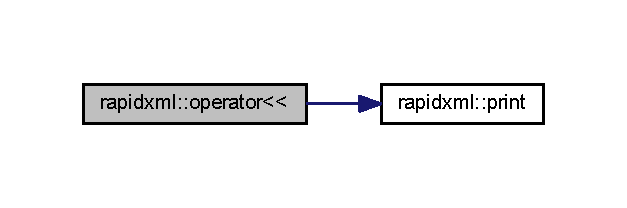
\includegraphics[width=301pt]{namespacerapidxml_a9ed8e626dd81348caede1f92a6c8418a_cgraph}
\end{center}
\end{figure}


\hypertarget{namespacerapidxml_a0fb0be6eba49fb2e2646d5a72a0dc355}{\index{rapidxml@{rapidxml}!print@{print}}
\index{print@{print}!rapidxml@{rapidxml}}
\subsubsection[{print}]{\setlength{\rightskip}{0pt plus 5cm}template$<$class Out\+It , class Ch $>$ Out\+It rapidxml\+::print (
\begin{DoxyParamCaption}
\item[{Out\+It}]{out, }
\item[{const xml\+\_\+node$<$ Ch $>$ \&}]{node, }
\item[{int}]{flags = {\ttfamily 0}}
\end{DoxyParamCaption}
)\hspace{0.3cm}{\ttfamily [inline]}}}\label{namespacerapidxml_a0fb0be6eba49fb2e2646d5a72a0dc355}
Prints X\+M\+L to given output iterator. 
\begin{DoxyParams}{Parameters}
{\em out} & Output iterator to print to. \\
\hline
{\em node} & Node to be printed. Pass \hyperlink{singletonrapidxml_1_1xml__document}{xml\+\_\+document} to print entire document. \\
\hline
{\em flags} & Flags controlling how X\+M\+L is printed. \\
\hline
\end{DoxyParams}
\begin{DoxyReturn}{Returns}
Output iterator pointing to position immediately after last character of printed text. 
\end{DoxyReturn}


Here is the caller graph for this function\+:
\nopagebreak
\begin{figure}[H]
\begin{center}
\leavevmode
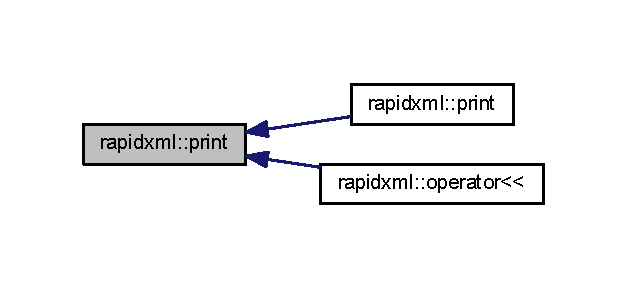
\includegraphics[width=301pt]{namespacerapidxml_a0fb0be6eba49fb2e2646d5a72a0dc355_icgraph}
\end{center}
\end{figure}


\hypertarget{namespacerapidxml_a0d2e114d5dd85e13c23b8dab600720fe}{\index{rapidxml@{rapidxml}!print@{print}}
\index{print@{print}!rapidxml@{rapidxml}}
\subsubsection[{print}]{\setlength{\rightskip}{0pt plus 5cm}template$<$class Ch $>$ std\+::basic\+\_\+ostream$<$Ch$>$\& rapidxml\+::print (
\begin{DoxyParamCaption}
\item[{std\+::basic\+\_\+ostream$<$ Ch $>$ \&}]{out, }
\item[{const xml\+\_\+node$<$ Ch $>$ \&}]{node, }
\item[{int}]{flags = {\ttfamily 0}}
\end{DoxyParamCaption}
)\hspace{0.3cm}{\ttfamily [inline]}}}\label{namespacerapidxml_a0d2e114d5dd85e13c23b8dab600720fe}
Prints X\+M\+L to given output stream. 
\begin{DoxyParams}{Parameters}
{\em out} & Output stream to print to. \\
\hline
{\em node} & Node to be printed. Pass \hyperlink{singletonrapidxml_1_1xml__document}{xml\+\_\+document} to print entire document. \\
\hline
{\em flags} & Flags controlling how X\+M\+L is printed. \\
\hline
\end{DoxyParams}
\begin{DoxyReturn}{Returns}
Output stream. 
\end{DoxyReturn}


Here is the call graph for this function\+:
\nopagebreak
\begin{figure}[H]
\begin{center}
\leavevmode
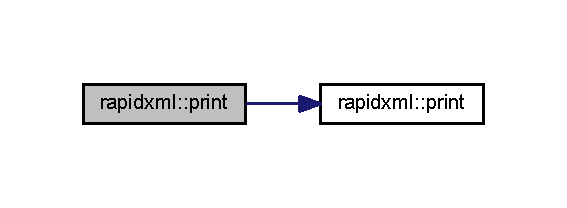
\includegraphics[width=272pt]{namespacerapidxml_a0d2e114d5dd85e13c23b8dab600720fe_cgraph}
\end{center}
\end{figure}




\subsection{Variable Documentation}
\hypertarget{namespacerapidxml_ae093dd49e2f59fa39eee95f1a6568e32}{\index{rapidxml@{rapidxml}!parse\+\_\+comment\+\_\+nodes@{parse\+\_\+comment\+\_\+nodes}}
\index{parse\+\_\+comment\+\_\+nodes@{parse\+\_\+comment\+\_\+nodes}!rapidxml@{rapidxml}}
\subsubsection[{parse\+\_\+comment\+\_\+nodes}]{\setlength{\rightskip}{0pt plus 5cm}const int rapidxml\+::parse\+\_\+comment\+\_\+nodes = 0x40}}\label{namespacerapidxml_ae093dd49e2f59fa39eee95f1a6568e32}
Parse flag instructing the parser to create comments nodes. By default, comment nodes are not created. Can be combined with other flags by use of $\vert$ operator. ~\newline
~\newline
 See \hyperlink{singletonrapidxml_1_1xml__document_ac6e73ff9ac323bf5a370c38feb03a6b1}{xml\+\_\+document\+::parse()} function. \hypertarget{namespacerapidxml_a999d782659513f8015ea4236e3204c42}{\index{rapidxml@{rapidxml}!parse\+\_\+declaration\+\_\+node@{parse\+\_\+declaration\+\_\+node}}
\index{parse\+\_\+declaration\+\_\+node@{parse\+\_\+declaration\+\_\+node}!rapidxml@{rapidxml}}
\subsubsection[{parse\+\_\+declaration\+\_\+node}]{\setlength{\rightskip}{0pt plus 5cm}const int rapidxml\+::parse\+\_\+declaration\+\_\+node = 0x20}}\label{namespacerapidxml_a999d782659513f8015ea4236e3204c42}
Parse flag instructing the parser to create X\+M\+L declaration node. By default, declaration node is not created. Can be combined with other flags by use of $\vert$ operator. ~\newline
~\newline
 See \hyperlink{singletonrapidxml_1_1xml__document_ac6e73ff9ac323bf5a370c38feb03a6b1}{xml\+\_\+document\+::parse()} function. \hypertarget{namespacerapidxml_acf4edf952f59eb1b6124ea37ad7da3ab}{\index{rapidxml@{rapidxml}!parse\+\_\+default@{parse\+\_\+default}}
\index{parse\+\_\+default@{parse\+\_\+default}!rapidxml@{rapidxml}}
\subsubsection[{parse\+\_\+default}]{\setlength{\rightskip}{0pt plus 5cm}const int rapidxml\+::parse\+\_\+default = 0}}\label{namespacerapidxml_acf4edf952f59eb1b6124ea37ad7da3ab}
Parse flags which represent default behaviour of the parser. This is always equal to 0, so that all other flags can be simply ored together. Normally there is no need to inconveniently disable flags by anding with their negated ($\sim$) values. This also means that meaning of each flag is a {\itshape negation} of the default setting. For example, if flag name is \hyperlink{namespacerapidxml_a22d4aefaceb00d7afabfef7107b108da}{rapidxml\+::parse\+\_\+no\+\_\+utf8}, it means that utf-\/8 is {\itshape enabled} by default, and using the flag will disable it. ~\newline
~\newline
 See \hyperlink{singletonrapidxml_1_1xml__document_ac6e73ff9ac323bf5a370c38feb03a6b1}{xml\+\_\+document\+::parse()} function. \hypertarget{namespacerapidxml_a41002b49780a90a0bbcc28ce8b895fe4}{\index{rapidxml@{rapidxml}!parse\+\_\+doctype\+\_\+node@{parse\+\_\+doctype\+\_\+node}}
\index{parse\+\_\+doctype\+\_\+node@{parse\+\_\+doctype\+\_\+node}!rapidxml@{rapidxml}}
\subsubsection[{parse\+\_\+doctype\+\_\+node}]{\setlength{\rightskip}{0pt plus 5cm}const int rapidxml\+::parse\+\_\+doctype\+\_\+node = 0x80}}\label{namespacerapidxml_a41002b49780a90a0bbcc28ce8b895fe4}
Parse flag instructing the parser to create D\+O\+C\+T\+Y\+P\+E node. By default, doctype node is not created. Although W3\+C specification allows at most one D\+O\+C\+T\+Y\+P\+E node, Rapid\+Xml will silently accept documents with more than one. Can be combined with other flags by use of $\vert$ operator. ~\newline
~\newline
 See \hyperlink{singletonrapidxml_1_1xml__document_ac6e73ff9ac323bf5a370c38feb03a6b1}{xml\+\_\+document\+::parse()} function. \hypertarget{namespacerapidxml_a64da06dfdab7c86ca954bda4fecb978f}{\index{rapidxml@{rapidxml}!parse\+\_\+fastest@{parse\+\_\+fastest}}
\index{parse\+\_\+fastest@{parse\+\_\+fastest}!rapidxml@{rapidxml}}
\subsubsection[{parse\+\_\+fastest}]{\setlength{\rightskip}{0pt plus 5cm}const int rapidxml\+::parse\+\_\+fastest = {\bf parse\+\_\+non\+\_\+destructive} $\vert$ {\bf parse\+\_\+no\+\_\+data\+\_\+nodes}}}\label{namespacerapidxml_a64da06dfdab7c86ca954bda4fecb978f}
A combination of parse flags resulting in fastest possible parsing, without sacrificing important data. ~\newline
~\newline
 See \hyperlink{singletonrapidxml_1_1xml__document_ac6e73ff9ac323bf5a370c38feb03a6b1}{xml\+\_\+document\+::parse()} function. \hypertarget{namespacerapidxml_abb48dc65db75d9e49734bc5bd2fabbfc}{\index{rapidxml@{rapidxml}!parse\+\_\+full@{parse\+\_\+full}}
\index{parse\+\_\+full@{parse\+\_\+full}!rapidxml@{rapidxml}}
\subsubsection[{parse\+\_\+full}]{\setlength{\rightskip}{0pt plus 5cm}const int rapidxml\+::parse\+\_\+full = {\bf parse\+\_\+declaration\+\_\+node} $\vert$ {\bf parse\+\_\+comment\+\_\+nodes} $\vert$ {\bf parse\+\_\+doctype\+\_\+node} $\vert$ {\bf parse\+\_\+pi\+\_\+nodes} $\vert$ {\bf parse\+\_\+validate\+\_\+closing\+\_\+tags}}}\label{namespacerapidxml_abb48dc65db75d9e49734bc5bd2fabbfc}
A combination of parse flags resulting in largest amount of data being extracted. This usually results in slowest parsing. ~\newline
~\newline
 See \hyperlink{singletonrapidxml_1_1xml__document_ac6e73ff9ac323bf5a370c38feb03a6b1}{xml\+\_\+document\+::parse()} function. \hypertarget{namespacerapidxml_ac2d21ef14a4e8936b94aca5d38b1a74d}{\index{rapidxml@{rapidxml}!parse\+\_\+no\+\_\+data\+\_\+nodes@{parse\+\_\+no\+\_\+data\+\_\+nodes}}
\index{parse\+\_\+no\+\_\+data\+\_\+nodes@{parse\+\_\+no\+\_\+data\+\_\+nodes}!rapidxml@{rapidxml}}
\subsubsection[{parse\+\_\+no\+\_\+data\+\_\+nodes}]{\setlength{\rightskip}{0pt plus 5cm}const int rapidxml\+::parse\+\_\+no\+\_\+data\+\_\+nodes = 0x1}}\label{namespacerapidxml_ac2d21ef14a4e8936b94aca5d38b1a74d}
Parse flag instructing the parser to not create data nodes. Text of first data node will still be placed in value of parent element, unless \hyperlink{namespacerapidxml_a00e6fea134b786ea6efeed1c8bc4a668}{rapidxml\+::parse\+\_\+no\+\_\+element\+\_\+values} flag is also specified. Can be combined with other flags by use of $\vert$ operator. ~\newline
~\newline
 See \hyperlink{singletonrapidxml_1_1xml__document_ac6e73ff9ac323bf5a370c38feb03a6b1}{xml\+\_\+document\+::parse()} function. \hypertarget{namespacerapidxml_a00e6fea134b786ea6efeed1c8bc4a668}{\index{rapidxml@{rapidxml}!parse\+\_\+no\+\_\+element\+\_\+values@{parse\+\_\+no\+\_\+element\+\_\+values}}
\index{parse\+\_\+no\+\_\+element\+\_\+values@{parse\+\_\+no\+\_\+element\+\_\+values}!rapidxml@{rapidxml}}
\subsubsection[{parse\+\_\+no\+\_\+element\+\_\+values}]{\setlength{\rightskip}{0pt plus 5cm}const int rapidxml\+::parse\+\_\+no\+\_\+element\+\_\+values = 0x2}}\label{namespacerapidxml_a00e6fea134b786ea6efeed1c8bc4a668}
Parse flag instructing the parser to not use text of first data node as a value of parent element. Can be combined with other flags by use of $\vert$ operator. Note that child data nodes of element node take precendence over its value when printing. That is, if element has one or more child data nodes {\itshape and} a value, the value will be ignored. Use \hyperlink{namespacerapidxml_ac2d21ef14a4e8936b94aca5d38b1a74d}{rapidxml\+::parse\+\_\+no\+\_\+data\+\_\+nodes} flag to prevent creation of data nodes if you want to manipulate data using values of elements. ~\newline
~\newline
 See \hyperlink{singletonrapidxml_1_1xml__document_ac6e73ff9ac323bf5a370c38feb03a6b1}{xml\+\_\+document\+::parse()} function. \hypertarget{namespacerapidxml_a89113c103ffaf77615d1aa330c8dcca8}{\index{rapidxml@{rapidxml}!parse\+\_\+no\+\_\+entity\+\_\+translation@{parse\+\_\+no\+\_\+entity\+\_\+translation}}
\index{parse\+\_\+no\+\_\+entity\+\_\+translation@{parse\+\_\+no\+\_\+entity\+\_\+translation}!rapidxml@{rapidxml}}
\subsubsection[{parse\+\_\+no\+\_\+entity\+\_\+translation}]{\setlength{\rightskip}{0pt plus 5cm}const int rapidxml\+::parse\+\_\+no\+\_\+entity\+\_\+translation = 0x8}}\label{namespacerapidxml_a89113c103ffaf77615d1aa330c8dcca8}
Parse flag instructing the parser to not translate entities in the source text. By default entities are translated, modifying source text. Can be combined with other flags by use of $\vert$ operator. ~\newline
~\newline
 See \hyperlink{singletonrapidxml_1_1xml__document_ac6e73ff9ac323bf5a370c38feb03a6b1}{xml\+\_\+document\+::parse()} function. \hypertarget{namespacerapidxml_af3fc88ba6bee33482a2db81b1da36ea1}{\index{rapidxml@{rapidxml}!parse\+\_\+no\+\_\+string\+\_\+terminators@{parse\+\_\+no\+\_\+string\+\_\+terminators}}
\index{parse\+\_\+no\+\_\+string\+\_\+terminators@{parse\+\_\+no\+\_\+string\+\_\+terminators}!rapidxml@{rapidxml}}
\subsubsection[{parse\+\_\+no\+\_\+string\+\_\+terminators}]{\setlength{\rightskip}{0pt plus 5cm}const int rapidxml\+::parse\+\_\+no\+\_\+string\+\_\+terminators = 0x4}}\label{namespacerapidxml_af3fc88ba6bee33482a2db81b1da36ea1}
Parse flag instructing the parser to not place zero terminators after strings in the source text. By default zero terminators are placed, modifying source text. Can be combined with other flags by use of $\vert$ operator. ~\newline
~\newline
 See \hyperlink{singletonrapidxml_1_1xml__document_ac6e73ff9ac323bf5a370c38feb03a6b1}{xml\+\_\+document\+::parse()} function. \hypertarget{namespacerapidxml_a22d4aefaceb00d7afabfef7107b108da}{\index{rapidxml@{rapidxml}!parse\+\_\+no\+\_\+utf8@{parse\+\_\+no\+\_\+utf8}}
\index{parse\+\_\+no\+\_\+utf8@{parse\+\_\+no\+\_\+utf8}!rapidxml@{rapidxml}}
\subsubsection[{parse\+\_\+no\+\_\+utf8}]{\setlength{\rightskip}{0pt plus 5cm}const int rapidxml\+::parse\+\_\+no\+\_\+utf8 = 0x10}}\label{namespacerapidxml_a22d4aefaceb00d7afabfef7107b108da}
Parse flag instructing the parser to disable U\+T\+F-\/8 handling and assume plain 8 bit characters. By default, U\+T\+F-\/8 handling is enabled. Can be combined with other flags by use of $\vert$ operator. ~\newline
~\newline
 See \hyperlink{singletonrapidxml_1_1xml__document_ac6e73ff9ac323bf5a370c38feb03a6b1}{xml\+\_\+document\+::parse()} function. \hypertarget{namespacerapidxml_a45d4d8fef551beaaba23a83b847fd6a3}{\index{rapidxml@{rapidxml}!parse\+\_\+non\+\_\+destructive@{parse\+\_\+non\+\_\+destructive}}
\index{parse\+\_\+non\+\_\+destructive@{parse\+\_\+non\+\_\+destructive}!rapidxml@{rapidxml}}
\subsubsection[{parse\+\_\+non\+\_\+destructive}]{\setlength{\rightskip}{0pt plus 5cm}const int rapidxml\+::parse\+\_\+non\+\_\+destructive = {\bf parse\+\_\+no\+\_\+string\+\_\+terminators} $\vert$ {\bf parse\+\_\+no\+\_\+entity\+\_\+translation}}}\label{namespacerapidxml_a45d4d8fef551beaaba23a83b847fd6a3}
A combination of parse flags that forbids any modifications of the source text. This also results in faster parsing. However, note that the following will occur\+: 
\begin{DoxyItemize}
\item names and values of nodes will not be zero terminated, you have to use \hyperlink{classrapidxml_1_1xml__base_a7e7f98b3d01e1eab8dc1ca69aad9af84}{xml\+\_\+base\+::name\+\_\+size()} and \hyperlink{classrapidxml_1_1xml__base_a9fcf201ed0915ac18dd43b0b5dcfaf32}{xml\+\_\+base\+::value\+\_\+size()} functions to determine where name and value ends 
\item entities will not be translated 
\item whitespace will not be normalized 
\end{DoxyItemize}See \hyperlink{singletonrapidxml_1_1xml__document_ac6e73ff9ac323bf5a370c38feb03a6b1}{xml\+\_\+document\+::parse()} function. \hypertarget{namespacerapidxml_a31f33885defb5176a7d99e524c35d386}{\index{rapidxml@{rapidxml}!parse\+\_\+normalize\+\_\+whitespace@{parse\+\_\+normalize\+\_\+whitespace}}
\index{parse\+\_\+normalize\+\_\+whitespace@{parse\+\_\+normalize\+\_\+whitespace}!rapidxml@{rapidxml}}
\subsubsection[{parse\+\_\+normalize\+\_\+whitespace}]{\setlength{\rightskip}{0pt plus 5cm}const int rapidxml\+::parse\+\_\+normalize\+\_\+whitespace = 0x800}}\label{namespacerapidxml_a31f33885defb5176a7d99e524c35d386}
Parse flag instructing the parser to condense all whitespace runs of data nodes to a single space character. Trimming of leading and trailing whitespace of data is controlled by \hyperlink{namespacerapidxml_a61912424b47db5038e726d4e1c22417f}{rapidxml\+::parse\+\_\+trim\+\_\+whitespace} flag. By default, whitespace is not normalized. If this flag is specified, source text will be modified. Can be combined with other flags by use of $\vert$ operator. ~\newline
~\newline
 See \hyperlink{singletonrapidxml_1_1xml__document_ac6e73ff9ac323bf5a370c38feb03a6b1}{xml\+\_\+document\+::parse()} function. \hypertarget{namespacerapidxml_a03fe68fcf5d28f38476e0fd31adecc4c}{\index{rapidxml@{rapidxml}!parse\+\_\+pi\+\_\+nodes@{parse\+\_\+pi\+\_\+nodes}}
\index{parse\+\_\+pi\+\_\+nodes@{parse\+\_\+pi\+\_\+nodes}!rapidxml@{rapidxml}}
\subsubsection[{parse\+\_\+pi\+\_\+nodes}]{\setlength{\rightskip}{0pt plus 5cm}const int rapidxml\+::parse\+\_\+pi\+\_\+nodes = 0x100}}\label{namespacerapidxml_a03fe68fcf5d28f38476e0fd31adecc4c}
Parse flag instructing the parser to create P\+I nodes. By default, P\+I nodes are not created. Can be combined with other flags by use of $\vert$ operator. ~\newline
~\newline
 See \hyperlink{singletonrapidxml_1_1xml__document_ac6e73ff9ac323bf5a370c38feb03a6b1}{xml\+\_\+document\+::parse()} function. \hypertarget{namespacerapidxml_a61912424b47db5038e726d4e1c22417f}{\index{rapidxml@{rapidxml}!parse\+\_\+trim\+\_\+whitespace@{parse\+\_\+trim\+\_\+whitespace}}
\index{parse\+\_\+trim\+\_\+whitespace@{parse\+\_\+trim\+\_\+whitespace}!rapidxml@{rapidxml}}
\subsubsection[{parse\+\_\+trim\+\_\+whitespace}]{\setlength{\rightskip}{0pt plus 5cm}const int rapidxml\+::parse\+\_\+trim\+\_\+whitespace = 0x400}}\label{namespacerapidxml_a61912424b47db5038e726d4e1c22417f}
Parse flag instructing the parser to trim all leading and trailing whitespace of data nodes. By default, whitespace is not trimmed. This flag does not cause the parser to modify source text. Can be combined with other flags by use of $\vert$ operator. ~\newline
~\newline
 See \hyperlink{singletonrapidxml_1_1xml__document_ac6e73ff9ac323bf5a370c38feb03a6b1}{xml\+\_\+document\+::parse()} function. \hypertarget{namespacerapidxml_a7ce8f40fda68338e20b56f41e48e49f3}{\index{rapidxml@{rapidxml}!parse\+\_\+validate\+\_\+closing\+\_\+tags@{parse\+\_\+validate\+\_\+closing\+\_\+tags}}
\index{parse\+\_\+validate\+\_\+closing\+\_\+tags@{parse\+\_\+validate\+\_\+closing\+\_\+tags}!rapidxml@{rapidxml}}
\subsubsection[{parse\+\_\+validate\+\_\+closing\+\_\+tags}]{\setlength{\rightskip}{0pt plus 5cm}const int rapidxml\+::parse\+\_\+validate\+\_\+closing\+\_\+tags = 0x200}}\label{namespacerapidxml_a7ce8f40fda68338e20b56f41e48e49f3}
Parse flag instructing the parser to validate closing tag names. If not set, name inside closing tag is irrelevant to the parser. By default, closing tags are not validated. Can be combined with other flags by use of $\vert$ operator. ~\newline
~\newline
 See \hyperlink{singletonrapidxml_1_1xml__document_ac6e73ff9ac323bf5a370c38feb03a6b1}{xml\+\_\+document\+::parse()} function. \hypertarget{namespacerapidxml_a65477b812a80f5bda693ec57e57de064}{\index{rapidxml@{rapidxml}!print\+\_\+no\+\_\+indenting@{print\+\_\+no\+\_\+indenting}}
\index{print\+\_\+no\+\_\+indenting@{print\+\_\+no\+\_\+indenting}!rapidxml@{rapidxml}}
\subsubsection[{print\+\_\+no\+\_\+indenting}]{\setlength{\rightskip}{0pt plus 5cm}const int rapidxml\+::print\+\_\+no\+\_\+indenting = 0x1}}\label{namespacerapidxml_a65477b812a80f5bda693ec57e57de064}


Printer flag instructing the printer to suppress indenting of X\+M\+L. See \hyperlink{namespacerapidxml_a0fb0be6eba49fb2e2646d5a72a0dc355}{print()} function. 


\chapter{Class Documentation}
\hypertarget{struct___w_d_i_r}{\section{\+\_\+\+W\+D\+I\+R Struct Reference}
\label{struct___w_d_i_r}\index{\+\_\+\+W\+D\+I\+R@{\+\_\+\+W\+D\+I\+R}}
}


{\ttfamily \#include $<$dirent.\+h$>$}



Collaboration diagram for \+\_\+\+W\+D\+I\+R\+:\nopagebreak
\begin{figure}[H]
\begin{center}
\leavevmode
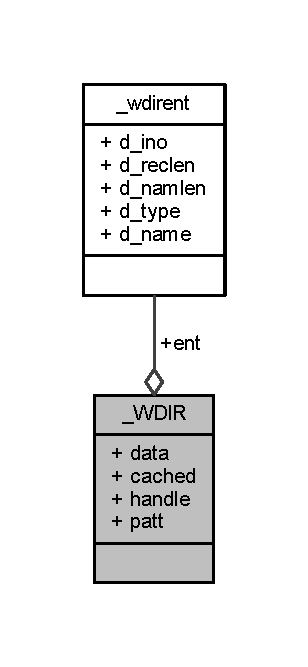
\includegraphics[width=148pt]{struct___w_d_i_r__coll__graph}
\end{center}
\end{figure}
\subsection*{Public Attributes}
\begin{DoxyCompactItemize}
\item 
struct \hyperlink{struct__wdirent}{\+\_\+wdirent} \hyperlink{struct___w_d_i_r_a84ae1457352005f813ed4b3dc1994b62}{ent}
\item 
W\+I\+N32\+\_\+\+F\+I\+N\+D\+\_\+\+D\+A\+T\+A\+W \hyperlink{struct___w_d_i_r_a065b17b666ee06c4e8068d8accb0eef9}{data}
\item 
int \hyperlink{struct___w_d_i_r_a9b7432df163d1e291ba5925347fd4af3}{cached}
\item 
H\+A\+N\+D\+L\+E \hyperlink{struct___w_d_i_r_a694510e166fd3e797b3e15b9e4b3810a}{handle}
\item 
wchar\+\_\+t $\ast$ \hyperlink{struct___w_d_i_r_a700ff3a1096fb36452c571b0f55b4e60}{patt}
\end{DoxyCompactItemize}


\subsection{Member Data Documentation}
\hypertarget{struct___w_d_i_r_a9b7432df163d1e291ba5925347fd4af3}{\index{\+\_\+\+W\+D\+I\+R@{\+\_\+\+W\+D\+I\+R}!cached@{cached}}
\index{cached@{cached}!\+\_\+\+W\+D\+I\+R@{\+\_\+\+W\+D\+I\+R}}
\subsubsection[{cached}]{\setlength{\rightskip}{0pt plus 5cm}int \+\_\+\+W\+D\+I\+R\+::cached}}\label{struct___w_d_i_r_a9b7432df163d1e291ba5925347fd4af3}
\hypertarget{struct___w_d_i_r_a065b17b666ee06c4e8068d8accb0eef9}{\index{\+\_\+\+W\+D\+I\+R@{\+\_\+\+W\+D\+I\+R}!data@{data}}
\index{data@{data}!\+\_\+\+W\+D\+I\+R@{\+\_\+\+W\+D\+I\+R}}
\subsubsection[{data}]{\setlength{\rightskip}{0pt plus 5cm}W\+I\+N32\+\_\+\+F\+I\+N\+D\+\_\+\+D\+A\+T\+A\+W \+\_\+\+W\+D\+I\+R\+::data}}\label{struct___w_d_i_r_a065b17b666ee06c4e8068d8accb0eef9}
\hypertarget{struct___w_d_i_r_a84ae1457352005f813ed4b3dc1994b62}{\index{\+\_\+\+W\+D\+I\+R@{\+\_\+\+W\+D\+I\+R}!ent@{ent}}
\index{ent@{ent}!\+\_\+\+W\+D\+I\+R@{\+\_\+\+W\+D\+I\+R}}
\subsubsection[{ent}]{\setlength{\rightskip}{0pt plus 5cm}struct {\bf \+\_\+wdirent} \+\_\+\+W\+D\+I\+R\+::ent}}\label{struct___w_d_i_r_a84ae1457352005f813ed4b3dc1994b62}
\hypertarget{struct___w_d_i_r_a694510e166fd3e797b3e15b9e4b3810a}{\index{\+\_\+\+W\+D\+I\+R@{\+\_\+\+W\+D\+I\+R}!handle@{handle}}
\index{handle@{handle}!\+\_\+\+W\+D\+I\+R@{\+\_\+\+W\+D\+I\+R}}
\subsubsection[{handle}]{\setlength{\rightskip}{0pt plus 5cm}H\+A\+N\+D\+L\+E \+\_\+\+W\+D\+I\+R\+::handle}}\label{struct___w_d_i_r_a694510e166fd3e797b3e15b9e4b3810a}
\hypertarget{struct___w_d_i_r_a700ff3a1096fb36452c571b0f55b4e60}{\index{\+\_\+\+W\+D\+I\+R@{\+\_\+\+W\+D\+I\+R}!patt@{patt}}
\index{patt@{patt}!\+\_\+\+W\+D\+I\+R@{\+\_\+\+W\+D\+I\+R}}
\subsubsection[{patt}]{\setlength{\rightskip}{0pt plus 5cm}wchar\+\_\+t$\ast$ \+\_\+\+W\+D\+I\+R\+::patt}}\label{struct___w_d_i_r_a700ff3a1096fb36452c571b0f55b4e60}


The documentation for this struct was generated from the following file\+:\begin{DoxyCompactItemize}
\item 
jamms/\+Tower\+Defense/\+Tower\+Defense/include/\hyperlink{dirent_8h}{dirent.\+h}\end{DoxyCompactItemize}

\hypertarget{struct__wdirent}{\section{\+\_\+wdirent Struct Reference}
\label{struct__wdirent}\index{\+\_\+wdirent@{\+\_\+wdirent}}
}


{\ttfamily \#include $<$dirent.\+h$>$}



Collaboration diagram for \+\_\+wdirent\+:\nopagebreak
\begin{figure}[H]
\begin{center}
\leavevmode
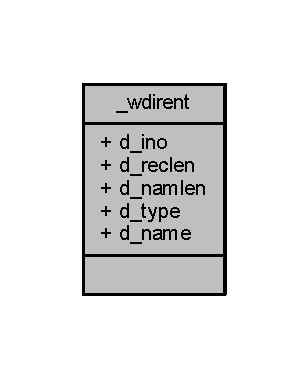
\includegraphics[width=148pt]{struct__wdirent__coll__graph}
\end{center}
\end{figure}
\subsection*{Public Attributes}
\begin{DoxyCompactItemize}
\item 
long \hyperlink{struct__wdirent_ac8cfaf294a0b6a49287d3f384c280c93}{d\+\_\+ino}
\item 
unsigned short \hyperlink{struct__wdirent_aff7f360608e576cd18cf11f2caf13ef3}{d\+\_\+reclen}
\item 
size\+\_\+t \hyperlink{struct__wdirent_a0050d6131e6fa90206903e216b38799e}{d\+\_\+namlen}
\item 
int \hyperlink{struct__wdirent_a3c3874604ffccbeeaffd96709763cc3b}{d\+\_\+type}
\item 
wchar\+\_\+t \hyperlink{struct__wdirent_a267f915cd36cad5969337a9192cab567}{d\+\_\+name} \mbox{[}\hyperlink{dirent_8h_ae688d728e1acdfe5988c7db45d6f0166}{P\+A\+T\+H\+\_\+\+M\+A\+X}\mbox{]}
\end{DoxyCompactItemize}


\subsection{Member Data Documentation}
\hypertarget{struct__wdirent_ac8cfaf294a0b6a49287d3f384c280c93}{\index{\+\_\+wdirent@{\+\_\+wdirent}!d\+\_\+ino@{d\+\_\+ino}}
\index{d\+\_\+ino@{d\+\_\+ino}!\+\_\+wdirent@{\+\_\+wdirent}}
\subsubsection[{d\+\_\+ino}]{\setlength{\rightskip}{0pt plus 5cm}long \+\_\+wdirent\+::d\+\_\+ino}}\label{struct__wdirent_ac8cfaf294a0b6a49287d3f384c280c93}
\hypertarget{struct__wdirent_a267f915cd36cad5969337a9192cab567}{\index{\+\_\+wdirent@{\+\_\+wdirent}!d\+\_\+name@{d\+\_\+name}}
\index{d\+\_\+name@{d\+\_\+name}!\+\_\+wdirent@{\+\_\+wdirent}}
\subsubsection[{d\+\_\+name}]{\setlength{\rightskip}{0pt plus 5cm}wchar\+\_\+t \+\_\+wdirent\+::d\+\_\+name\mbox{[}{\bf P\+A\+T\+H\+\_\+\+M\+A\+X}\mbox{]}}}\label{struct__wdirent_a267f915cd36cad5969337a9192cab567}
\hypertarget{struct__wdirent_a0050d6131e6fa90206903e216b38799e}{\index{\+\_\+wdirent@{\+\_\+wdirent}!d\+\_\+namlen@{d\+\_\+namlen}}
\index{d\+\_\+namlen@{d\+\_\+namlen}!\+\_\+wdirent@{\+\_\+wdirent}}
\subsubsection[{d\+\_\+namlen}]{\setlength{\rightskip}{0pt plus 5cm}size\+\_\+t \+\_\+wdirent\+::d\+\_\+namlen}}\label{struct__wdirent_a0050d6131e6fa90206903e216b38799e}
\hypertarget{struct__wdirent_aff7f360608e576cd18cf11f2caf13ef3}{\index{\+\_\+wdirent@{\+\_\+wdirent}!d\+\_\+reclen@{d\+\_\+reclen}}
\index{d\+\_\+reclen@{d\+\_\+reclen}!\+\_\+wdirent@{\+\_\+wdirent}}
\subsubsection[{d\+\_\+reclen}]{\setlength{\rightskip}{0pt plus 5cm}unsigned short \+\_\+wdirent\+::d\+\_\+reclen}}\label{struct__wdirent_aff7f360608e576cd18cf11f2caf13ef3}
\hypertarget{struct__wdirent_a3c3874604ffccbeeaffd96709763cc3b}{\index{\+\_\+wdirent@{\+\_\+wdirent}!d\+\_\+type@{d\+\_\+type}}
\index{d\+\_\+type@{d\+\_\+type}!\+\_\+wdirent@{\+\_\+wdirent}}
\subsubsection[{d\+\_\+type}]{\setlength{\rightskip}{0pt plus 5cm}int \+\_\+wdirent\+::d\+\_\+type}}\label{struct__wdirent_a3c3874604ffccbeeaffd96709763cc3b}


The documentation for this struct was generated from the following file\+:\begin{DoxyCompactItemize}
\item 
jamms/\+Tower\+Defense/\+Tower\+Defense/include/\hyperlink{dirent_8h}{dirent.\+h}\end{DoxyCompactItemize}

\hypertarget{class_animation}{\section{Animation Class Reference}
\label{class_animation}\index{Animation@{Animation}}
}


Represents an animation in the game.  




{\ttfamily \#include $<$Animation.\+h$>$}



Collaboration diagram for Animation\+:\nopagebreak
\begin{figure}[H]
\begin{center}
\leavevmode
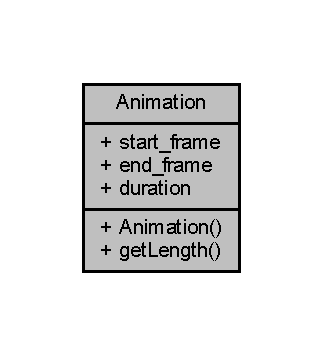
\includegraphics[width=155pt]{class_animation__coll__graph}
\end{center}
\end{figure}
\subsection*{Public Member Functions}
\begin{DoxyCompactItemize}
\item 
\hyperlink{class_animation_a35f74d462e717b7f65917a5259183db8}{Animation} (unsigned int \hyperlink{class_animation_a22f5936a58ca1850d5232a1cbfcb3426}{start\+\_\+frame}, unsigned int \hyperlink{class_animation_a4dcf93e9ee175acaa8cc84f3241e8ee0}{end\+\_\+frame}, float \hyperlink{class_animation_a66cc7333638f071b0401072ba95c55fd}{duration})
\begin{DoxyCompactList}\small\item\em \hyperlink{class_animation}{Animation} constructor. \end{DoxyCompactList}\item 
unsigned int \hyperlink{class_animation_ad0967bfc76be3a06a17ad774b50dc97e}{get\+Length} ()
\begin{DoxyCompactList}\small\item\em Returns the length of the animation. \end{DoxyCompactList}\end{DoxyCompactItemize}
\subsection*{Public Attributes}
\begin{DoxyCompactItemize}
\item 
unsigned int \hyperlink{class_animation_a22f5936a58ca1850d5232a1cbfcb3426}{start\+\_\+frame}
\begin{DoxyCompactList}\small\item\em Index of start frame in the sprite sheet. \end{DoxyCompactList}\item 
unsigned int \hyperlink{class_animation_a4dcf93e9ee175acaa8cc84f3241e8ee0}{end\+\_\+frame}
\begin{DoxyCompactList}\small\item\em Index of end frame in the sprite sheet. \end{DoxyCompactList}\item 
float \hyperlink{class_animation_a66cc7333638f071b0401072ba95c55fd}{duration}
\begin{DoxyCompactList}\small\item\em Amount of time one frame of the animation should last for. \end{DoxyCompactList}\end{DoxyCompactItemize}


\subsection{Detailed Description}
Represents an animation in the game. 

\subsection{Constructor \& Destructor Documentation}
\hypertarget{class_animation_a35f74d462e717b7f65917a5259183db8}{\index{Animation@{Animation}!Animation@{Animation}}
\index{Animation@{Animation}!Animation@{Animation}}
\subsubsection[{Animation}]{\setlength{\rightskip}{0pt plus 5cm}Animation\+::\+Animation (
\begin{DoxyParamCaption}
\item[{unsigned int}]{start\+\_\+frame, }
\item[{unsigned int}]{end\+\_\+frame, }
\item[{float}]{duration}
\end{DoxyParamCaption}
)\hspace{0.3cm}{\ttfamily [inline]}}}\label{class_animation_a35f74d462e717b7f65917a5259183db8}


\hyperlink{class_animation}{Animation} constructor. 


\begin{DoxyParams}{Parameters}
{\em start\+\_\+frame} & Start frame index \\
\hline
{\em end\+\_\+fram} & End frame index \\
\hline
{\em duration} & How long one frame of the animation lasts \\
\hline
\end{DoxyParams}


\subsection{Member Function Documentation}
\hypertarget{class_animation_ad0967bfc76be3a06a17ad774b50dc97e}{\index{Animation@{Animation}!get\+Length@{get\+Length}}
\index{get\+Length@{get\+Length}!Animation@{Animation}}
\subsubsection[{get\+Length}]{\setlength{\rightskip}{0pt plus 5cm}unsigned int Animation\+::get\+Length (
\begin{DoxyParamCaption}
{}
\end{DoxyParamCaption}
)\hspace{0.3cm}{\ttfamily [inline]}}}\label{class_animation_ad0967bfc76be3a06a17ad774b50dc97e}


Returns the length of the animation. 


\begin{DoxyParams}{Parameters}
{\em Unsigned} & int representing the length of animation in frames \\
\hline
\end{DoxyParams}


\subsection{Member Data Documentation}
\hypertarget{class_animation_a66cc7333638f071b0401072ba95c55fd}{\index{Animation@{Animation}!duration@{duration}}
\index{duration@{duration}!Animation@{Animation}}
\subsubsection[{duration}]{\setlength{\rightskip}{0pt plus 5cm}float Animation\+::duration}}\label{class_animation_a66cc7333638f071b0401072ba95c55fd}


Amount of time one frame of the animation should last for. 

\hypertarget{class_animation_a4dcf93e9ee175acaa8cc84f3241e8ee0}{\index{Animation@{Animation}!end\+\_\+frame@{end\+\_\+frame}}
\index{end\+\_\+frame@{end\+\_\+frame}!Animation@{Animation}}
\subsubsection[{end\+\_\+frame}]{\setlength{\rightskip}{0pt plus 5cm}unsigned int Animation\+::end\+\_\+frame}}\label{class_animation_a4dcf93e9ee175acaa8cc84f3241e8ee0}


Index of end frame in the sprite sheet. 

\hypertarget{class_animation_a22f5936a58ca1850d5232a1cbfcb3426}{\index{Animation@{Animation}!start\+\_\+frame@{start\+\_\+frame}}
\index{start\+\_\+frame@{start\+\_\+frame}!Animation@{Animation}}
\subsubsection[{start\+\_\+frame}]{\setlength{\rightskip}{0pt plus 5cm}unsigned int Animation\+::start\+\_\+frame}}\label{class_animation_a22f5936a58ca1850d5232a1cbfcb3426}


Index of start frame in the sprite sheet. 



The documentation for this class was generated from the following file\+:\begin{DoxyCompactItemize}
\item 
jamms/\+Tower\+Defense/\+Tower\+Defense/include/utils/\hyperlink{_animation_8h}{Animation.\+h}\end{DoxyCompactItemize}

\hypertarget{class_animation_handler}{\section{Animation\+Handler Class Reference}
\label{class_animation_handler}\index{Animation\+Handler@{Animation\+Handler}}
}


Handles animations.  




{\ttfamily \#include $<$Animation\+Handler.\+h$>$}



Collaboration diagram for Animation\+Handler\+:
\nopagebreak
\begin{figure}[H]
\begin{center}
\leavevmode
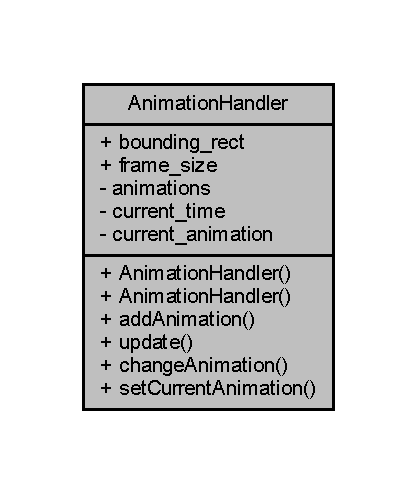
\includegraphics[width=200pt]{class_animation_handler__coll__graph}
\end{center}
\end{figure}
\subsection*{Public Member Functions}
\begin{DoxyCompactItemize}
\item 
\hyperlink{class_animation_handler_ae10c29a1cb88b70f31034da4b863098c}{Animation\+Handler} ()
\begin{DoxyCompactList}\small\item\em \hyperlink{class_animation_handler}{Animation\+Handler} constructor. \end{DoxyCompactList}\item 
\hyperlink{class_animation_handler_a4d7522e516b77aa5ebd9340561156369}{Animation\+Handler} (const sf\+::\+Int\+Rect \&\hyperlink{class_animation_handler_a8615fd6169591c5788c9f6a83cdf0ec7}{frame\+\_\+size})
\begin{DoxyCompactList}\small\item\em Overloading \hyperlink{class_animation_handler}{Animation\+Handler} constructor with frame size. \end{DoxyCompactList}\item 
void \hyperlink{class_animation_handler_ae517a14ed199418ccbc8d71db5ad5955}{add\+Animation} (\hyperlink{class_animation}{Animation} \&animation)
\begin{DoxyCompactList}\small\item\em Add a new animation. \end{DoxyCompactList}\item 
void \hyperlink{class_animation_handler_a74c541905109998e971c578c4aa3e3de}{update} (const float delta\+\_\+time)
\begin{DoxyCompactList}\small\item\em Updates the current frame of animation. \end{DoxyCompactList}\item 
void \hyperlink{class_animation_handler_a93f1509e5eccdf13a07ba1eb2256c6d0}{change\+Animation} (unsigned int animation\+\_\+index)
\begin{DoxyCompactList}\small\item\em Changes the animation. \end{DoxyCompactList}\item 
void \hyperlink{class_animation_handler_ae9cc10dd30d2c48eedb400d32b6eb4b6}{set\+Current\+Animation} (float \hyperlink{class_animation_handler_ad03db9fa9c9589a72b438033b283a9cb}{current\+\_\+animation})
\end{DoxyCompactItemize}
\subsection*{Public Attributes}
\begin{DoxyCompactItemize}
\item 
sf\+::\+Int\+Rect \hyperlink{class_animation_handler_ae38964052ccbdd44d92c8d23eb0b880d}{bounding\+\_\+rect}
\begin{DoxyCompactList}\small\item\em Current section of the texture to be displayed. \end{DoxyCompactList}\item 
sf\+::\+Int\+Rect \hyperlink{class_animation_handler_a8615fd6169591c5788c9f6a83cdf0ec7}{frame\+\_\+size}
\begin{DoxyCompactList}\small\item\em Pixel dimensions of each animation frame. \end{DoxyCompactList}\end{DoxyCompactItemize}
\subsection*{Private Attributes}
\begin{DoxyCompactItemize}
\item 
std\+::vector$<$ \hyperlink{class_animation}{Animation} $>$ \hyperlink{class_animation_handler_ab04e2b457325095c264dba4a067690cd}{animations}
\begin{DoxyCompactList}\small\item\em Array of animations. \end{DoxyCompactList}\item 
float \hyperlink{class_animation_handler_a91dd0c9aeb1b824a2ddef6b6867a0245}{current\+\_\+time}
\begin{DoxyCompactList}\small\item\em Time since the animation loop started. \end{DoxyCompactList}\item 
int \hyperlink{class_animation_handler_ad03db9fa9c9589a72b438033b283a9cb}{current\+\_\+animation}
\begin{DoxyCompactList}\small\item\em Current animation displayed. \end{DoxyCompactList}\end{DoxyCompactItemize}


\subsection{Detailed Description}
Handles animations. 

\subsection{Constructor \& Destructor Documentation}
\hypertarget{class_animation_handler_ae10c29a1cb88b70f31034da4b863098c}{\index{Animation\+Handler@{Animation\+Handler}!Animation\+Handler@{Animation\+Handler}}
\index{Animation\+Handler@{Animation\+Handler}!Animation\+Handler@{Animation\+Handler}}
\subsubsection[{Animation\+Handler}]{\setlength{\rightskip}{0pt plus 5cm}Animation\+Handler\+::\+Animation\+Handler (
\begin{DoxyParamCaption}
{}
\end{DoxyParamCaption}
)\hspace{0.3cm}{\ttfamily [inline]}}}\label{class_animation_handler_ae10c29a1cb88b70f31034da4b863098c}


\hyperlink{class_animation_handler}{Animation\+Handler} constructor. 

\hypertarget{class_animation_handler_a4d7522e516b77aa5ebd9340561156369}{\index{Animation\+Handler@{Animation\+Handler}!Animation\+Handler@{Animation\+Handler}}
\index{Animation\+Handler@{Animation\+Handler}!Animation\+Handler@{Animation\+Handler}}
\subsubsection[{Animation\+Handler}]{\setlength{\rightskip}{0pt plus 5cm}Animation\+Handler\+::\+Animation\+Handler (
\begin{DoxyParamCaption}
\item[{const sf\+::\+Int\+Rect \&}]{frame\+\_\+size}
\end{DoxyParamCaption}
)\hspace{0.3cm}{\ttfamily [inline]}}}\label{class_animation_handler_a4d7522e516b77aa5ebd9340561156369}


Overloading \hyperlink{class_animation_handler}{Animation\+Handler} constructor with frame size. 



\subsection{Member Function Documentation}
\hypertarget{class_animation_handler_ae517a14ed199418ccbc8d71db5ad5955}{\index{Animation\+Handler@{Animation\+Handler}!add\+Animation@{add\+Animation}}
\index{add\+Animation@{add\+Animation}!Animation\+Handler@{Animation\+Handler}}
\subsubsection[{add\+Animation}]{\setlength{\rightskip}{0pt plus 5cm}void Animation\+Handler\+::add\+Animation (
\begin{DoxyParamCaption}
\item[{{\bf Animation} \&}]{animation}
\end{DoxyParamCaption}
)}}\label{class_animation_handler_ae517a14ed199418ccbc8d71db5ad5955}


Add a new animation. 

\begin{DoxyReturn}{Returns}
Void. 
\end{DoxyReturn}


Here is the caller graph for this function\+:
\nopagebreak
\begin{figure}[H]
\begin{center}
\leavevmode
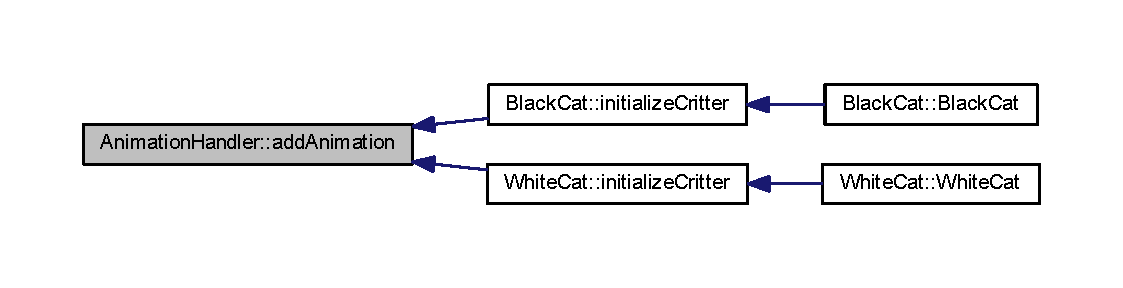
\includegraphics[width=350pt]{class_animation_handler_ae517a14ed199418ccbc8d71db5ad5955_icgraph}
\end{center}
\end{figure}


\hypertarget{class_animation_handler_a93f1509e5eccdf13a07ba1eb2256c6d0}{\index{Animation\+Handler@{Animation\+Handler}!change\+Animation@{change\+Animation}}
\index{change\+Animation@{change\+Animation}!Animation\+Handler@{Animation\+Handler}}
\subsubsection[{change\+Animation}]{\setlength{\rightskip}{0pt plus 5cm}void Animation\+Handler\+::change\+Animation (
\begin{DoxyParamCaption}
\item[{unsigned int}]{animation\+\_\+index}
\end{DoxyParamCaption}
)}}\label{class_animation_handler_a93f1509e5eccdf13a07ba1eb2256c6d0}


Changes the animation. 


\begin{DoxyParams}{Parameters}
{\em animation\+\_\+index} & Index of new animation. \\
\hline
\end{DoxyParams}
\begin{DoxyReturn}{Returns}
Void.
\end{DoxyReturn}
The \hyperlink{class_animation_handler_a93f1509e5eccdf13a07ba1eb2256c6d0}{change\+Animation()} function sets the current animation to the new animation if the new animation is valid. If the new animation is set, elapsed time is reset. 

Here is the caller graph for this function\+:
\nopagebreak
\begin{figure}[H]
\begin{center}
\leavevmode
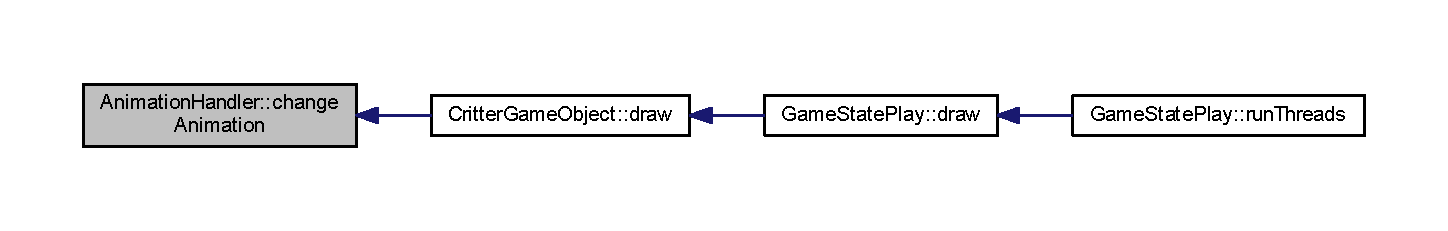
\includegraphics[width=350pt]{class_animation_handler_a93f1509e5eccdf13a07ba1eb2256c6d0_icgraph}
\end{center}
\end{figure}


\hypertarget{class_animation_handler_ae9cc10dd30d2c48eedb400d32b6eb4b6}{\index{Animation\+Handler@{Animation\+Handler}!set\+Current\+Animation@{set\+Current\+Animation}}
\index{set\+Current\+Animation@{set\+Current\+Animation}!Animation\+Handler@{Animation\+Handler}}
\subsubsection[{set\+Current\+Animation}]{\setlength{\rightskip}{0pt plus 5cm}void Animation\+Handler\+::set\+Current\+Animation (
\begin{DoxyParamCaption}
\item[{float}]{current\+\_\+animation}
\end{DoxyParamCaption}
)\hspace{0.3cm}{\ttfamily [inline]}}}\label{class_animation_handler_ae9cc10dd30d2c48eedb400d32b6eb4b6}
\hypertarget{class_animation_handler_a74c541905109998e971c578c4aa3e3de}{\index{Animation\+Handler@{Animation\+Handler}!update@{update}}
\index{update@{update}!Animation\+Handler@{Animation\+Handler}}
\subsubsection[{update}]{\setlength{\rightskip}{0pt plus 5cm}void Animation\+Handler\+::update (
\begin{DoxyParamCaption}
\item[{const float}]{delta\+\_\+time}
\end{DoxyParamCaption}
)}}\label{class_animation_handler_a74c541905109998e971c578c4aa3e3de}


Updates the current frame of animation. 


\begin{DoxyParams}{Parameters}
{\em delta\+\_\+time} & Time since the update was last called (i.\+e. time for one frame to be executed). \\
\hline
\end{DoxyParams}
\begin{DoxyReturn}{Returns}
Void.
\end{DoxyReturn}
The \hyperlink{class_animation_handler_a74c541905109998e971c578c4aa3e3de}{update()} function calculates and sets up the next frame for the animation. It also keeps track of elapsed time. 

Here is the caller graph for this function\+:
\nopagebreak
\begin{figure}[H]
\begin{center}
\leavevmode
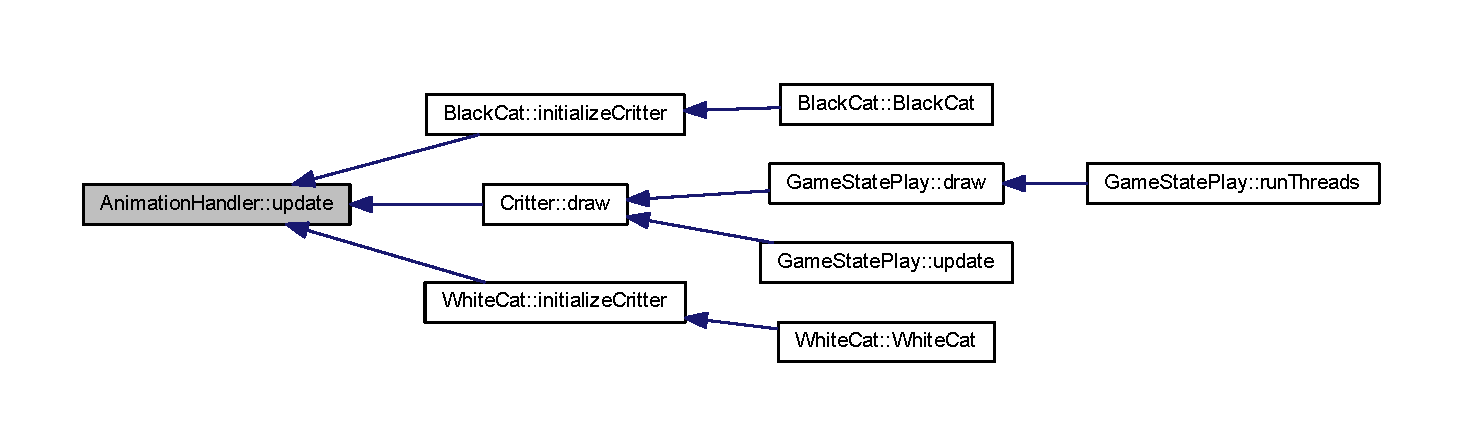
\includegraphics[width=350pt]{class_animation_handler_a74c541905109998e971c578c4aa3e3de_icgraph}
\end{center}
\end{figure}




\subsection{Member Data Documentation}
\hypertarget{class_animation_handler_ab04e2b457325095c264dba4a067690cd}{\index{Animation\+Handler@{Animation\+Handler}!animations@{animations}}
\index{animations@{animations}!Animation\+Handler@{Animation\+Handler}}
\subsubsection[{animations}]{\setlength{\rightskip}{0pt plus 5cm}std\+::vector$<${\bf Animation}$>$ Animation\+Handler\+::animations\hspace{0.3cm}{\ttfamily [private]}}}\label{class_animation_handler_ab04e2b457325095c264dba4a067690cd}


Array of animations. 

\hypertarget{class_animation_handler_ae38964052ccbdd44d92c8d23eb0b880d}{\index{Animation\+Handler@{Animation\+Handler}!bounding\+\_\+rect@{bounding\+\_\+rect}}
\index{bounding\+\_\+rect@{bounding\+\_\+rect}!Animation\+Handler@{Animation\+Handler}}
\subsubsection[{bounding\+\_\+rect}]{\setlength{\rightskip}{0pt plus 5cm}sf\+::\+Int\+Rect Animation\+Handler\+::bounding\+\_\+rect}}\label{class_animation_handler_ae38964052ccbdd44d92c8d23eb0b880d}


Current section of the texture to be displayed. 

\hypertarget{class_animation_handler_ad03db9fa9c9589a72b438033b283a9cb}{\index{Animation\+Handler@{Animation\+Handler}!current\+\_\+animation@{current\+\_\+animation}}
\index{current\+\_\+animation@{current\+\_\+animation}!Animation\+Handler@{Animation\+Handler}}
\subsubsection[{current\+\_\+animation}]{\setlength{\rightskip}{0pt plus 5cm}int Animation\+Handler\+::current\+\_\+animation\hspace{0.3cm}{\ttfamily [private]}}}\label{class_animation_handler_ad03db9fa9c9589a72b438033b283a9cb}


Current animation displayed. 

\hypertarget{class_animation_handler_a91dd0c9aeb1b824a2ddef6b6867a0245}{\index{Animation\+Handler@{Animation\+Handler}!current\+\_\+time@{current\+\_\+time}}
\index{current\+\_\+time@{current\+\_\+time}!Animation\+Handler@{Animation\+Handler}}
\subsubsection[{current\+\_\+time}]{\setlength{\rightskip}{0pt plus 5cm}float Animation\+Handler\+::current\+\_\+time\hspace{0.3cm}{\ttfamily [private]}}}\label{class_animation_handler_a91dd0c9aeb1b824a2ddef6b6867a0245}


Time since the animation loop started. 

\hypertarget{class_animation_handler_a8615fd6169591c5788c9f6a83cdf0ec7}{\index{Animation\+Handler@{Animation\+Handler}!frame\+\_\+size@{frame\+\_\+size}}
\index{frame\+\_\+size@{frame\+\_\+size}!Animation\+Handler@{Animation\+Handler}}
\subsubsection[{frame\+\_\+size}]{\setlength{\rightskip}{0pt plus 5cm}sf\+::\+Int\+Rect Animation\+Handler\+::frame\+\_\+size}}\label{class_animation_handler_a8615fd6169591c5788c9f6a83cdf0ec7}


Pixel dimensions of each animation frame. 



The documentation for this class was generated from the following files\+:\begin{DoxyCompactItemize}
\item 
jamms/\+Tower\+Defense/\+Tower\+Defense/include/utils/\hyperlink{_animation_handler_8h}{Animation\+Handler.\+h}\item 
jamms/\+Tower\+Defense/\+Tower\+Defense/src/utils/\hyperlink{_animation_handler_8cpp}{Animation\+Handler.\+cpp}\end{DoxyCompactItemize}

\hypertarget{structrapidxml_1_1xml__document_1_1attribute__name__pred}{\section{rapidxml\+:\+:xml\+\_\+document$<$ Ch $>$\+:\+:attribute\+\_\+name\+\_\+pred Struct Reference}
\label{structrapidxml_1_1xml__document_1_1attribute__name__pred}\index{rapidxml\+::xml\+\_\+document$<$ Ch $>$\+::attribute\+\_\+name\+\_\+pred@{rapidxml\+::xml\+\_\+document$<$ Ch $>$\+::attribute\+\_\+name\+\_\+pred}}
}


Collaboration diagram for rapidxml\+:\+:xml\+\_\+document$<$ Ch $>$\+:\+:attribute\+\_\+name\+\_\+pred\+:
\nopagebreak
\begin{figure}[H]
\begin{center}
\leavevmode
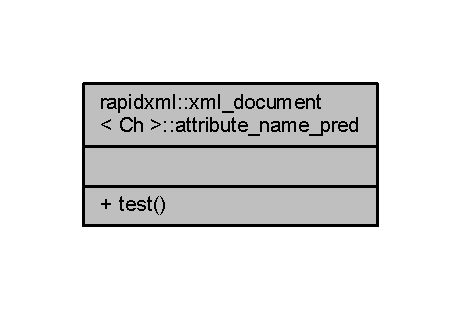
\includegraphics[width=221pt]{structrapidxml_1_1xml__document_1_1attribute__name__pred__coll__graph}
\end{center}
\end{figure}
\subsection*{Static Public Member Functions}
\begin{DoxyCompactItemize}
\item 
static unsigned char \hyperlink{structrapidxml_1_1xml__document_1_1attribute__name__pred_a2cf003483847dfabcf0c83877818a4c5}{test} (Ch ch)
\end{DoxyCompactItemize}


\subsection{Member Function Documentation}
\hypertarget{structrapidxml_1_1xml__document_1_1attribute__name__pred_a2cf003483847dfabcf0c83877818a4c5}{\index{rapidxml\+::xml\+\_\+document\+::attribute\+\_\+name\+\_\+pred@{rapidxml\+::xml\+\_\+document\+::attribute\+\_\+name\+\_\+pred}!test@{test}}
\index{test@{test}!rapidxml\+::xml\+\_\+document\+::attribute\+\_\+name\+\_\+pred@{rapidxml\+::xml\+\_\+document\+::attribute\+\_\+name\+\_\+pred}}
\subsubsection[{test}]{\setlength{\rightskip}{0pt plus 5cm}template$<$class Ch  = char$>$ static unsigned char {\bf rapidxml\+::xml\+\_\+document}$<$ Ch $>$\+::attribute\+\_\+name\+\_\+pred\+::test (
\begin{DoxyParamCaption}
\item[{Ch}]{ch}
\end{DoxyParamCaption}
)\hspace{0.3cm}{\ttfamily [inline]}, {\ttfamily [static]}}}\label{structrapidxml_1_1xml__document_1_1attribute__name__pred_a2cf003483847dfabcf0c83877818a4c5}


Here is the caller graph for this function\+:
\nopagebreak
\begin{figure}[H]
\begin{center}
\leavevmode
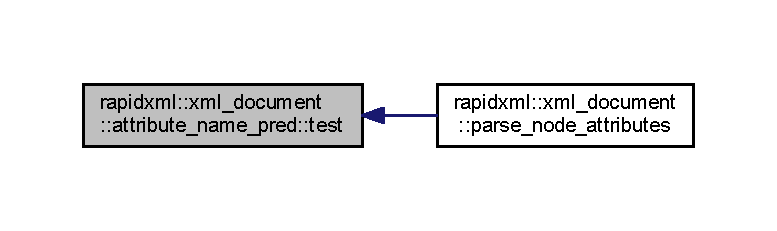
\includegraphics[width=350pt]{structrapidxml_1_1xml__document_1_1attribute__name__pred_a2cf003483847dfabcf0c83877818a4c5_icgraph}
\end{center}
\end{figure}




The documentation for this struct was generated from the following file\+:\begin{DoxyCompactItemize}
\item 
jamms/\+Tower\+Defense/\+Tower\+Defense/include/utils/\hyperlink{rapidxml_8hpp}{rapidxml.\+hpp}\end{DoxyCompactItemize}

\hypertarget{structrapidxml_1_1xml__document_1_1attribute__value__pred}{\section{rapidxml\+:\+:xml\+\_\+document$<$ Ch $>$\+:\+:attribute\+\_\+value\+\_\+pred$<$ Quote $>$ Struct Template Reference}
\label{structrapidxml_1_1xml__document_1_1attribute__value__pred}\index{rapidxml\+::xml\+\_\+document$<$ Ch $>$\+::attribute\+\_\+value\+\_\+pred$<$ Quote $>$@{rapidxml\+::xml\+\_\+document$<$ Ch $>$\+::attribute\+\_\+value\+\_\+pred$<$ Quote $>$}}
}


Collaboration diagram for rapidxml\+:\+:xml\+\_\+document$<$ Ch $>$\+:\+:attribute\+\_\+value\+\_\+pred$<$ Quote $>$\+:\nopagebreak
\begin{figure}[H]
\begin{center}
\leavevmode
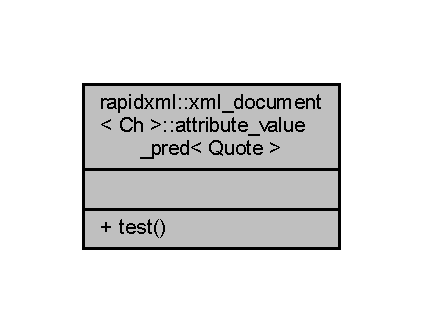
\includegraphics[width=203pt]{structrapidxml_1_1xml__document_1_1attribute__value__pred__coll__graph}
\end{center}
\end{figure}
\subsection*{Static Public Member Functions}
\begin{DoxyCompactItemize}
\item 
static unsigned char \hyperlink{structrapidxml_1_1xml__document_1_1attribute__value__pred_a1c81901177c96057b2808747fc62f9c5}{test} (Ch ch)
\end{DoxyCompactItemize}


\subsection{Member Function Documentation}
\hypertarget{structrapidxml_1_1xml__document_1_1attribute__value__pred_a1c81901177c96057b2808747fc62f9c5}{\index{rapidxml\+::xml\+\_\+document\+::attribute\+\_\+value\+\_\+pred@{rapidxml\+::xml\+\_\+document\+::attribute\+\_\+value\+\_\+pred}!test@{test}}
\index{test@{test}!rapidxml\+::xml\+\_\+document\+::attribute\+\_\+value\+\_\+pred@{rapidxml\+::xml\+\_\+document\+::attribute\+\_\+value\+\_\+pred}}
\subsubsection[{test}]{\setlength{\rightskip}{0pt plus 5cm}template$<$class Ch  = char$>$ template$<$Ch Quote$>$ static unsigned char {\bf rapidxml\+::xml\+\_\+document}$<$ Ch $>$\+::{\bf attribute\+\_\+value\+\_\+pred}$<$ Quote $>$\+::test (
\begin{DoxyParamCaption}
\item[{Ch}]{ch}
\end{DoxyParamCaption}
)\hspace{0.3cm}{\ttfamily [inline]}, {\ttfamily [static]}}}\label{structrapidxml_1_1xml__document_1_1attribute__value__pred_a1c81901177c96057b2808747fc62f9c5}


The documentation for this struct was generated from the following file\+:\begin{DoxyCompactItemize}
\item 
jamms/\+Tower\+Defense/\+Tower\+Defense/include/utils/\hyperlink{rapidxml_8hpp}{rapidxml.\+hpp}\end{DoxyCompactItemize}

\hypertarget{structrapidxml_1_1xml__document_1_1attribute__value__pure__pred}{\section{rapidxml\+:\+:xml\+\_\+document$<$ Ch $>$\+:\+:attribute\+\_\+value\+\_\+pure\+\_\+pred$<$ Quote $>$ Struct Template Reference}
\label{structrapidxml_1_1xml__document_1_1attribute__value__pure__pred}\index{rapidxml\+::xml\+\_\+document$<$ Ch $>$\+::attribute\+\_\+value\+\_\+pure\+\_\+pred$<$ Quote $>$@{rapidxml\+::xml\+\_\+document$<$ Ch $>$\+::attribute\+\_\+value\+\_\+pure\+\_\+pred$<$ Quote $>$}}
}


Collaboration diagram for rapidxml\+:\+:xml\+\_\+document$<$ Ch $>$\+:\+:attribute\+\_\+value\+\_\+pure\+\_\+pred$<$ Quote $>$\+:
\nopagebreak
\begin{figure}[H]
\begin{center}
\leavevmode
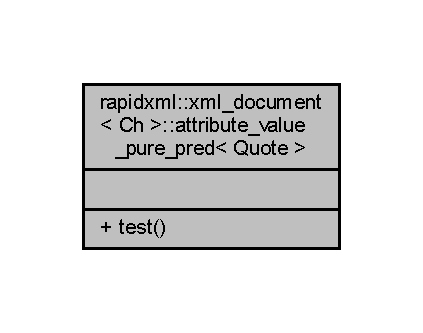
\includegraphics[width=203pt]{structrapidxml_1_1xml__document_1_1attribute__value__pure__pred__coll__graph}
\end{center}
\end{figure}
\subsection*{Static Public Member Functions}
\begin{DoxyCompactItemize}
\item 
static unsigned char \hyperlink{structrapidxml_1_1xml__document_1_1attribute__value__pure__pred_a3add4f66f917381562355d5f8b8917c1}{test} (Ch ch)
\end{DoxyCompactItemize}


\subsection{Member Function Documentation}
\hypertarget{structrapidxml_1_1xml__document_1_1attribute__value__pure__pred_a3add4f66f917381562355d5f8b8917c1}{\index{rapidxml\+::xml\+\_\+document\+::attribute\+\_\+value\+\_\+pure\+\_\+pred@{rapidxml\+::xml\+\_\+document\+::attribute\+\_\+value\+\_\+pure\+\_\+pred}!test@{test}}
\index{test@{test}!rapidxml\+::xml\+\_\+document\+::attribute\+\_\+value\+\_\+pure\+\_\+pred@{rapidxml\+::xml\+\_\+document\+::attribute\+\_\+value\+\_\+pure\+\_\+pred}}
\subsubsection[{test}]{\setlength{\rightskip}{0pt plus 5cm}template$<$class Ch  = char$>$ template$<$Ch Quote$>$ static unsigned char {\bf rapidxml\+::xml\+\_\+document}$<$ Ch $>$\+::{\bf attribute\+\_\+value\+\_\+pure\+\_\+pred}$<$ Quote $>$\+::test (
\begin{DoxyParamCaption}
\item[{Ch}]{ch}
\end{DoxyParamCaption}
)\hspace{0.3cm}{\ttfamily [inline]}, {\ttfamily [static]}}}\label{structrapidxml_1_1xml__document_1_1attribute__value__pure__pred_a3add4f66f917381562355d5f8b8917c1}


The documentation for this struct was generated from the following file\+:\begin{DoxyCompactItemize}
\item 
jamms/\+Tower\+Defense/\+Tower\+Defense/include/utils/\hyperlink{rapidxml_8hpp}{rapidxml.\+hpp}\end{DoxyCompactItemize}

\hypertarget{class_black_cat}{\section{Black\+Cat Class Reference}
\label{class_black_cat}\index{Black\+Cat@{Black\+Cat}}
}


Class for \hyperlink{class_black_cat}{Black\+Cat}. Subclass of \hyperlink{class_critter}{Critter}.  




{\ttfamily \#include $<$Black\+Cat.\+h$>$}



Inheritance diagram for Black\+Cat\+:
\nopagebreak
\begin{figure}[H]
\begin{center}
\leavevmode
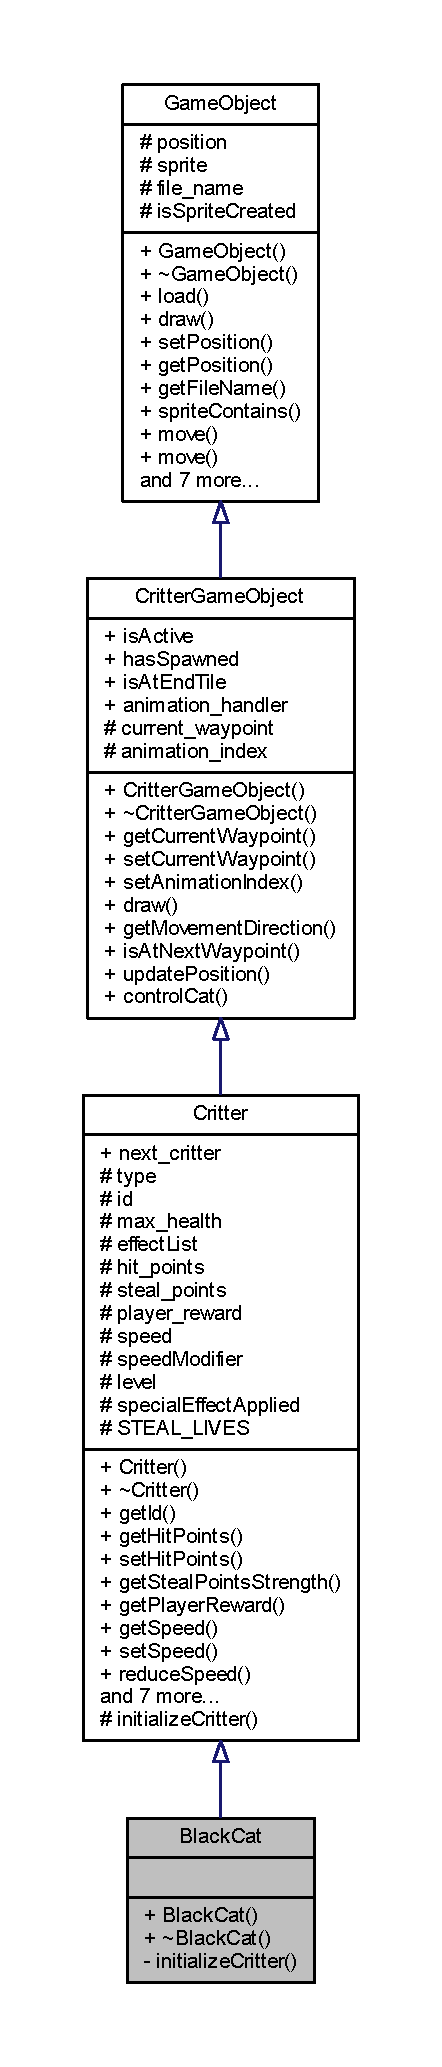
\includegraphics[height=550pt]{class_black_cat__inherit__graph}
\end{center}
\end{figure}


Collaboration diagram for Black\+Cat\+:
\nopagebreak
\begin{figure}[H]
\begin{center}
\leavevmode
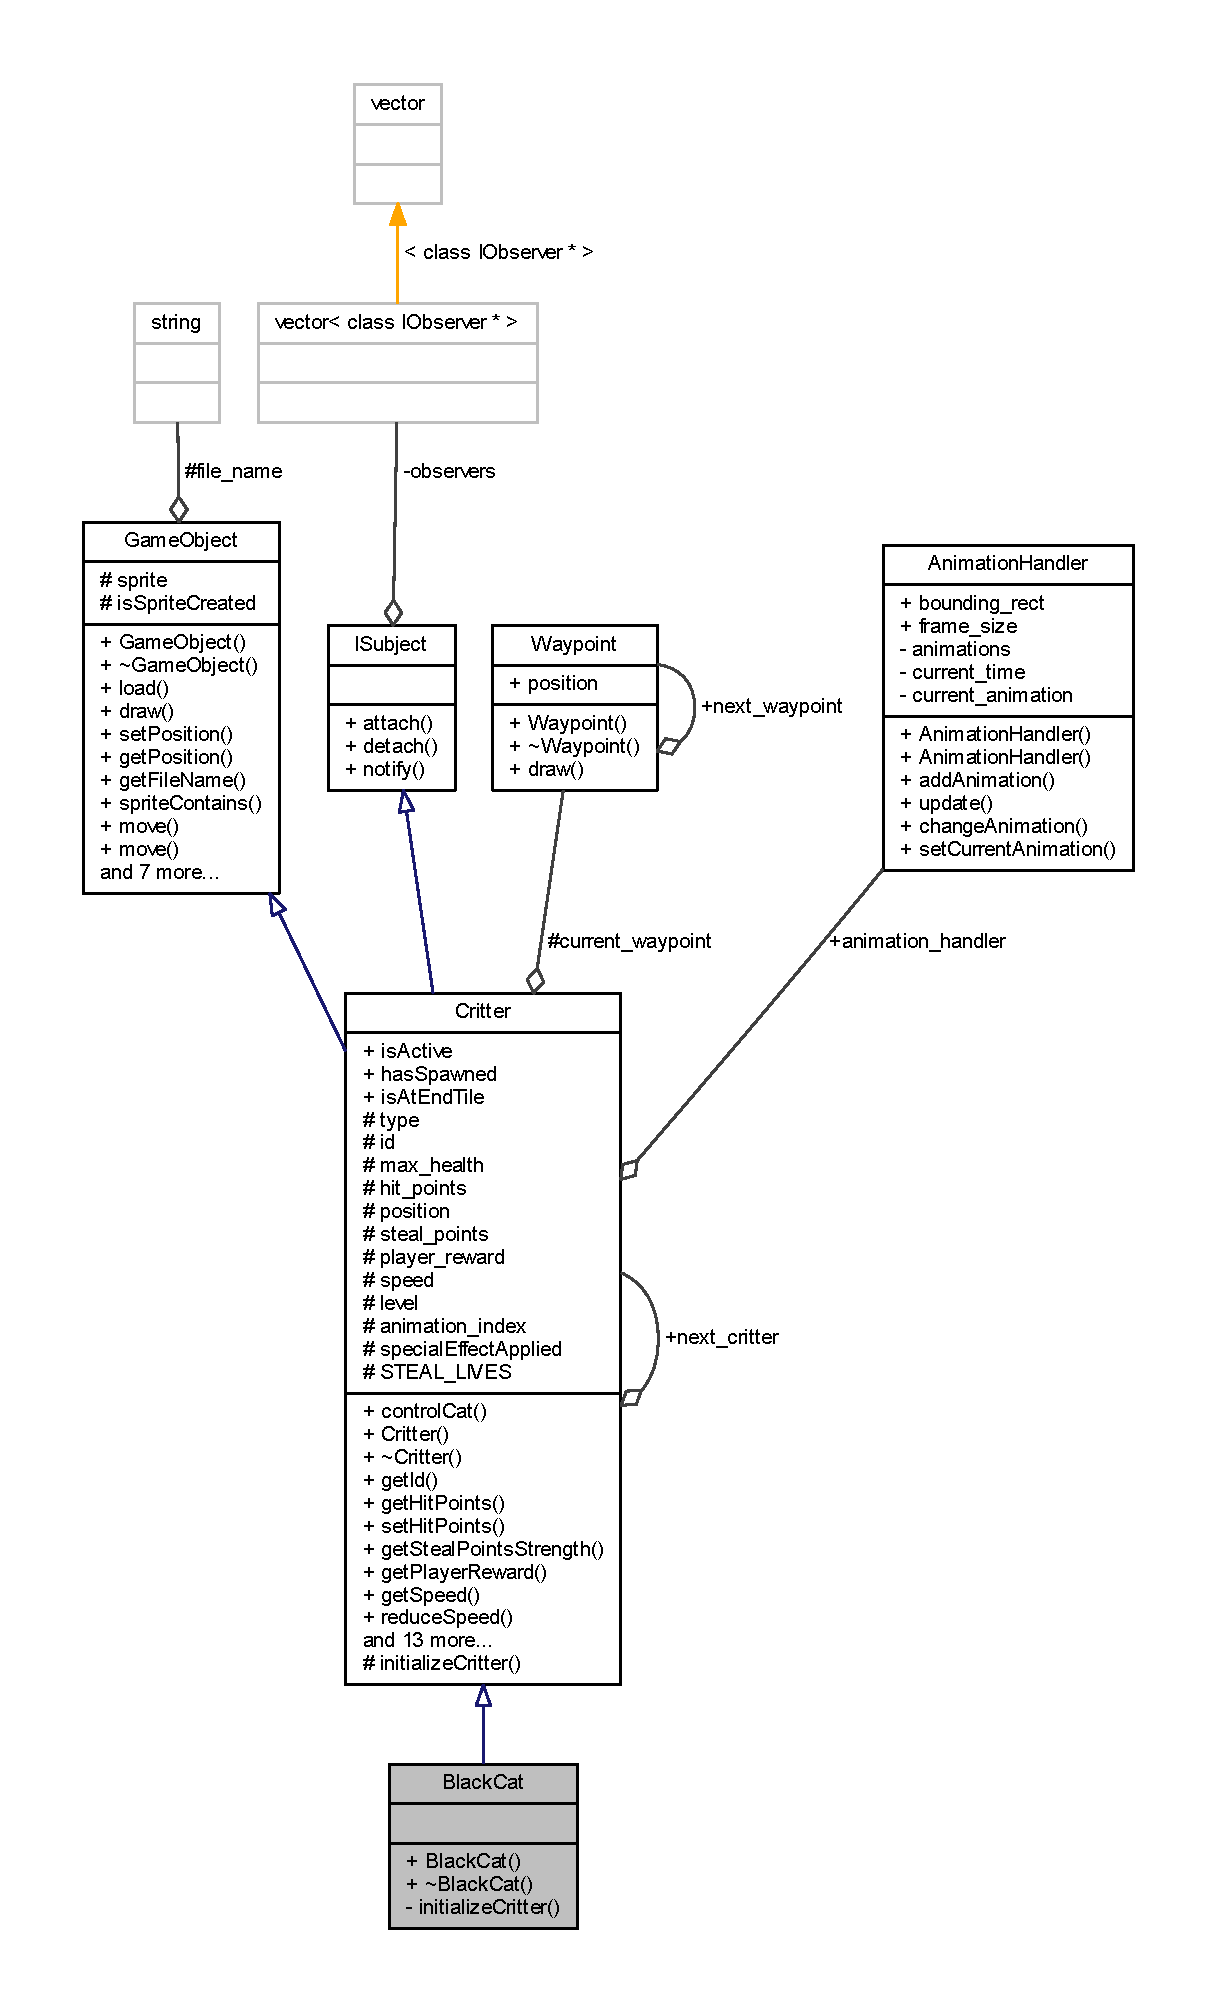
\includegraphics[height=550pt]{class_black_cat__coll__graph}
\end{center}
\end{figure}
\subsection*{Public Member Functions}
\begin{DoxyCompactItemize}
\item 
\hyperlink{class_black_cat_a7974aa98721932e53102c10484af1abe}{Black\+Cat} (int \hyperlink{class_critter_ae775e0ebe6e8bbe249c403670bda46f8}{id}, \hyperlink{class_waypoint}{Waypoint} $\ast$starting\+\_\+waypoint)
\begin{DoxyCompactList}\small\item\em The \hyperlink{class_black_cat}{Black\+Cat} constructor. Calls \hyperlink{class_black_cat_a2ae946e05f754f7d7bdbc753946425eb}{initialize\+Critter()} to set attributes of the \hyperlink{class_black_cat}{Black\+Cat} object. \end{DoxyCompactList}\item 
\hyperlink{class_black_cat_ae2d3786e829242eb070ce3adc41d7173}{$\sim$\+Black\+Cat} ()
\end{DoxyCompactItemize}
\subsection*{Private Member Functions}
\begin{DoxyCompactItemize}
\item 
virtual void \hyperlink{class_black_cat_a2ae946e05f754f7d7bdbc753946425eb}{initialize\+Critter} (const std\+::vector$<$ \hyperlink{class_animation}{Animation} $>$ \&animations)
\begin{DoxyCompactList}\small\item\em Initialization function for a \hyperlink{class_black_cat}{Black\+Cat}. \end{DoxyCompactList}\end{DoxyCompactItemize}
\subsection*{Additional Inherited Members}


\subsection{Detailed Description}
Class for \hyperlink{class_black_cat}{Black\+Cat}. Subclass of \hyperlink{class_critter}{Critter}. 

\subsection{Constructor \& Destructor Documentation}
\hypertarget{class_black_cat_a7974aa98721932e53102c10484af1abe}{\index{Black\+Cat@{Black\+Cat}!Black\+Cat@{Black\+Cat}}
\index{Black\+Cat@{Black\+Cat}!Black\+Cat@{Black\+Cat}}
\subsubsection[{Black\+Cat}]{\setlength{\rightskip}{0pt plus 5cm}Black\+Cat\+::\+Black\+Cat (
\begin{DoxyParamCaption}
\item[{int}]{id, }
\item[{{\bf Waypoint} $\ast$}]{starting\+\_\+waypoint}
\end{DoxyParamCaption}
)}}\label{class_black_cat_a7974aa98721932e53102c10484af1abe}


The \hyperlink{class_black_cat}{Black\+Cat} constructor. Calls \hyperlink{class_black_cat_a2ae946e05f754f7d7bdbc753946425eb}{initialize\+Critter()} to set attributes of the \hyperlink{class_black_cat}{Black\+Cat} object. 



Here is the call graph for this function\+:
\nopagebreak
\begin{figure}[H]
\begin{center}
\leavevmode
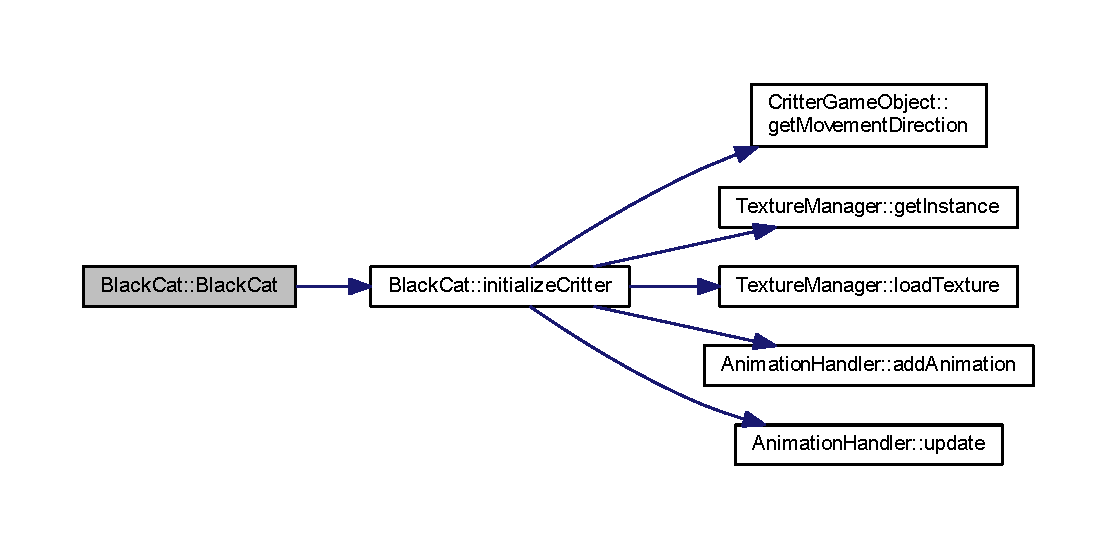
\includegraphics[width=350pt]{class_black_cat_a7974aa98721932e53102c10484af1abe_cgraph}
\end{center}
\end{figure}


\hypertarget{class_black_cat_ae2d3786e829242eb070ce3adc41d7173}{\index{Black\+Cat@{Black\+Cat}!````~Black\+Cat@{$\sim$\+Black\+Cat}}
\index{````~Black\+Cat@{$\sim$\+Black\+Cat}!Black\+Cat@{Black\+Cat}}
\subsubsection[{$\sim$\+Black\+Cat}]{\setlength{\rightskip}{0pt plus 5cm}Black\+Cat\+::$\sim$\+Black\+Cat (
\begin{DoxyParamCaption}
{}
\end{DoxyParamCaption}
)\hspace{0.3cm}{\ttfamily [inline]}}}\label{class_black_cat_ae2d3786e829242eb070ce3adc41d7173}


\subsection{Member Function Documentation}
\hypertarget{class_black_cat_a2ae946e05f754f7d7bdbc753946425eb}{\index{Black\+Cat@{Black\+Cat}!initialize\+Critter@{initialize\+Critter}}
\index{initialize\+Critter@{initialize\+Critter}!Black\+Cat@{Black\+Cat}}
\subsubsection[{initialize\+Critter}]{\setlength{\rightskip}{0pt plus 5cm}void Black\+Cat\+::initialize\+Critter (
\begin{DoxyParamCaption}
\item[{const std\+::vector$<$ {\bf Animation} $>$ \&}]{animations}
\end{DoxyParamCaption}
)\hspace{0.3cm}{\ttfamily [private]}, {\ttfamily [virtual]}}}\label{class_black_cat_a2ae946e05f754f7d7bdbc753946425eb}


Initialization function for a \hyperlink{class_black_cat}{Black\+Cat}. 


\begin{DoxyParams}{Parameters}
{\em animations} & Array of specified animations \\
\hline
\end{DoxyParams}
\begin{DoxyReturn}{Returns}
Void.
\end{DoxyReturn}
Initialization specific to a \hyperlink{class_black_cat}{Black\+Cat} object 

Implements \hyperlink{class_critter_ad425da71f01445ee175e5f98d94ca0ba}{Critter}.



Here is the call graph for this function\+:
\nopagebreak
\begin{figure}[H]
\begin{center}
\leavevmode
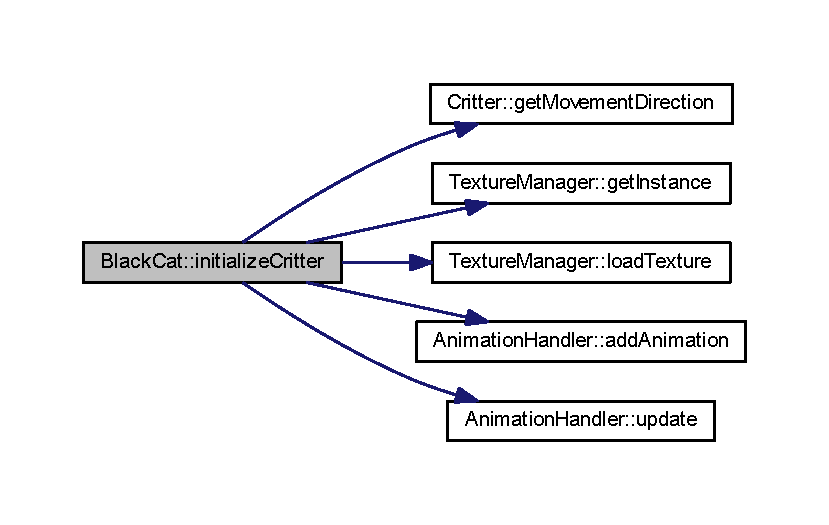
\includegraphics[width=350pt]{class_black_cat_a2ae946e05f754f7d7bdbc753946425eb_cgraph}
\end{center}
\end{figure}




Here is the caller graph for this function\+:
\nopagebreak
\begin{figure}[H]
\begin{center}
\leavevmode
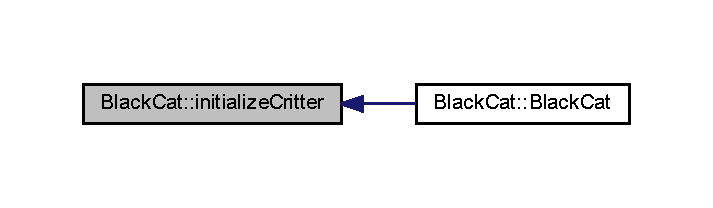
\includegraphics[width=342pt]{class_black_cat_a2ae946e05f754f7d7bdbc753946425eb_icgraph}
\end{center}
\end{figure}




The documentation for this class was generated from the following files\+:\begin{DoxyCompactItemize}
\item 
jamms/\+Tower\+Defense/\+Tower\+Defense/include/game\+Objects/\hyperlink{_black_cat_8h}{Black\+Cat.\+h}\item 
jamms/\+Tower\+Defense/\+Tower\+Defense/src/game\+Objects/\hyperlink{_black_cat_8cpp}{Black\+Cat.\+cpp}\end{DoxyCompactItemize}

\hypertarget{class_bulldog}{\section{Bulldog Class Reference}
\label{class_bulldog}\index{Bulldog@{Bulldog}}
}


{\ttfamily \#include $<$Bulldog.\+h$>$}



Inheritance diagram for Bulldog\+:
\nopagebreak
\begin{figure}[H]
\begin{center}
\leavevmode
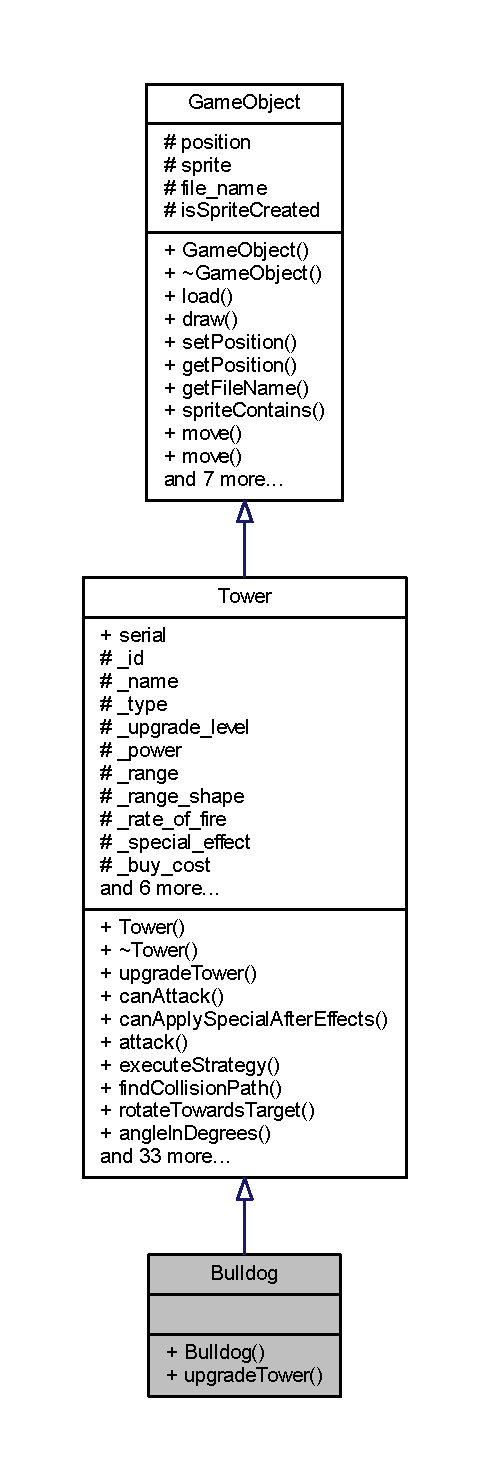
\includegraphics[height=550pt]{class_bulldog__inherit__graph}
\end{center}
\end{figure}


Collaboration diagram for Bulldog\+:
\nopagebreak
\begin{figure}[H]
\begin{center}
\leavevmode
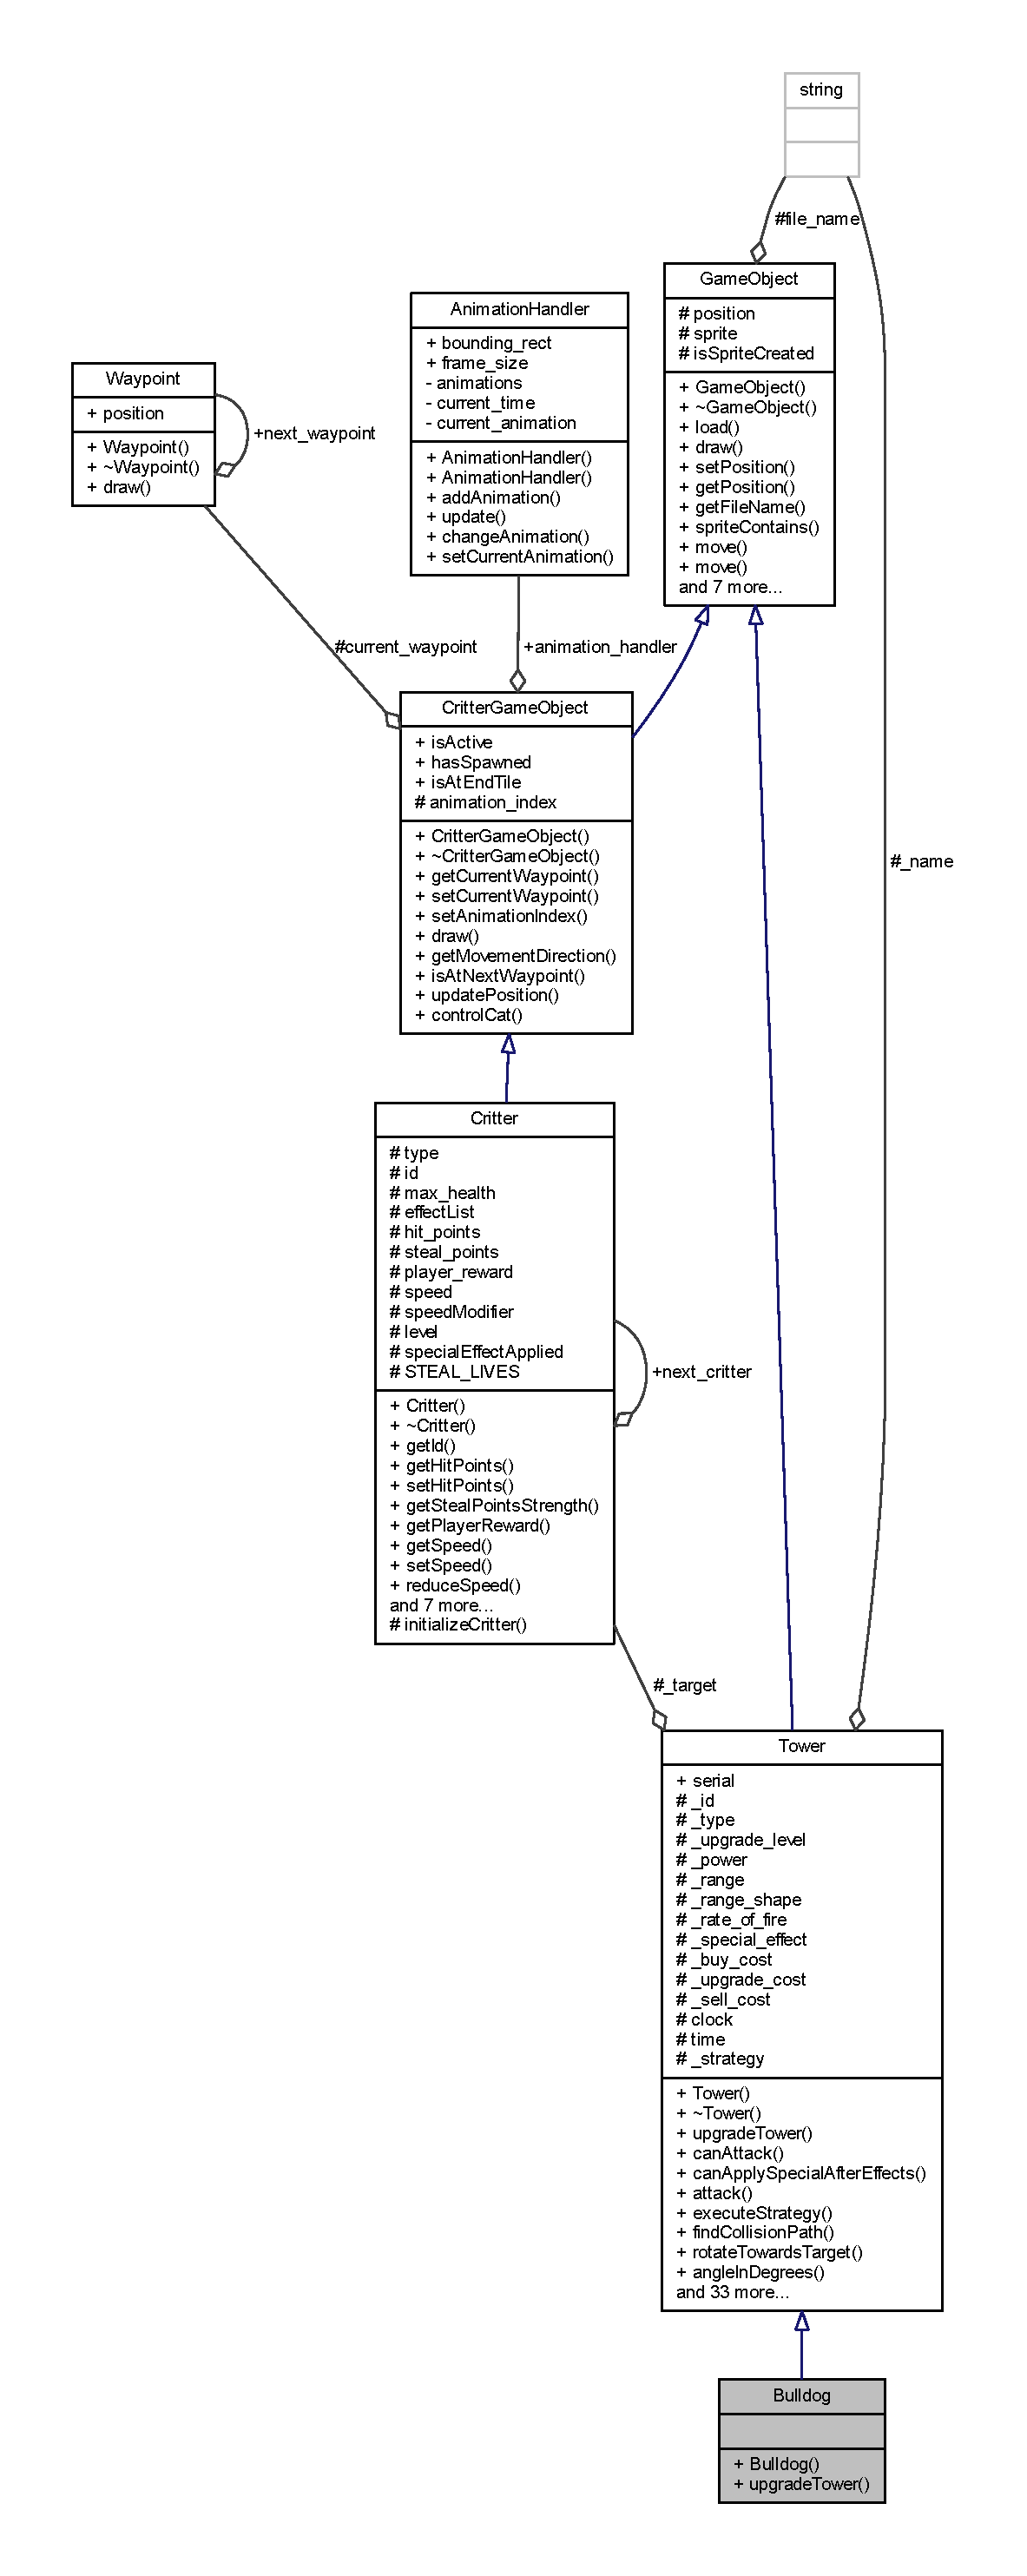
\includegraphics[height=550pt]{class_bulldog__coll__graph}
\end{center}
\end{figure}
\subsection*{Public Member Functions}
\begin{DoxyCompactItemize}
\item 
\hyperlink{class_bulldog_a21e6065a0e9cfa5aa862c8b7a5e1b88c}{Bulldog} (int tile\+X, int tile\+Y)
\item 
void \hyperlink{class_bulldog_adfecd22f881be0d7946534c2012275d7}{upgrade\+Tower} ()
\end{DoxyCompactItemize}
\subsection*{Additional Inherited Members}


\subsection{Constructor \& Destructor Documentation}
\hypertarget{class_bulldog_a21e6065a0e9cfa5aa862c8b7a5e1b88c}{\index{Bulldog@{Bulldog}!Bulldog@{Bulldog}}
\index{Bulldog@{Bulldog}!Bulldog@{Bulldog}}
\subsubsection[{Bulldog}]{\setlength{\rightskip}{0pt plus 5cm}Bulldog\+::\+Bulldog (
\begin{DoxyParamCaption}
\item[{int}]{tile\+X, }
\item[{int}]{tile\+Y}
\end{DoxyParamCaption}
)}}\label{class_bulldog_a21e6065a0e9cfa5aa862c8b7a5e1b88c}


Here is the call graph for this function\+:
\nopagebreak
\begin{figure}[H]
\begin{center}
\leavevmode
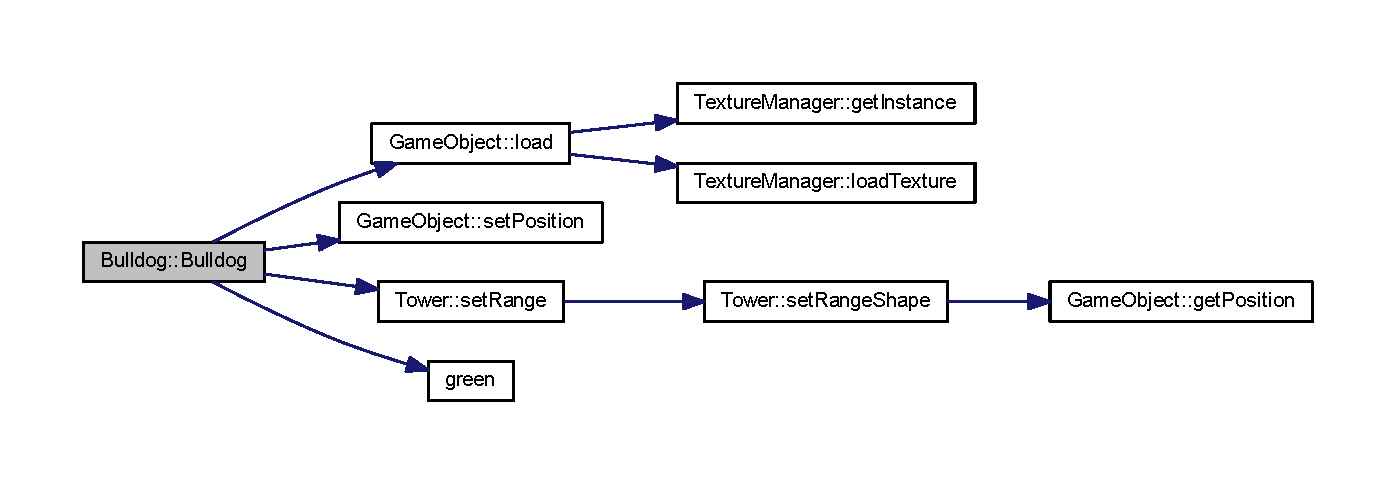
\includegraphics[width=350pt]{class_bulldog_a21e6065a0e9cfa5aa862c8b7a5e1b88c_cgraph}
\end{center}
\end{figure}




\subsection{Member Function Documentation}
\hypertarget{class_bulldog_adfecd22f881be0d7946534c2012275d7}{\index{Bulldog@{Bulldog}!upgrade\+Tower@{upgrade\+Tower}}
\index{upgrade\+Tower@{upgrade\+Tower}!Bulldog@{Bulldog}}
\subsubsection[{upgrade\+Tower}]{\setlength{\rightskip}{0pt plus 5cm}void Bulldog\+::upgrade\+Tower (
\begin{DoxyParamCaption}
{}
\end{DoxyParamCaption}
)}}\label{class_bulldog_adfecd22f881be0d7946534c2012275d7}


Here is the call graph for this function\+:
\nopagebreak
\begin{figure}[H]
\begin{center}
\leavevmode
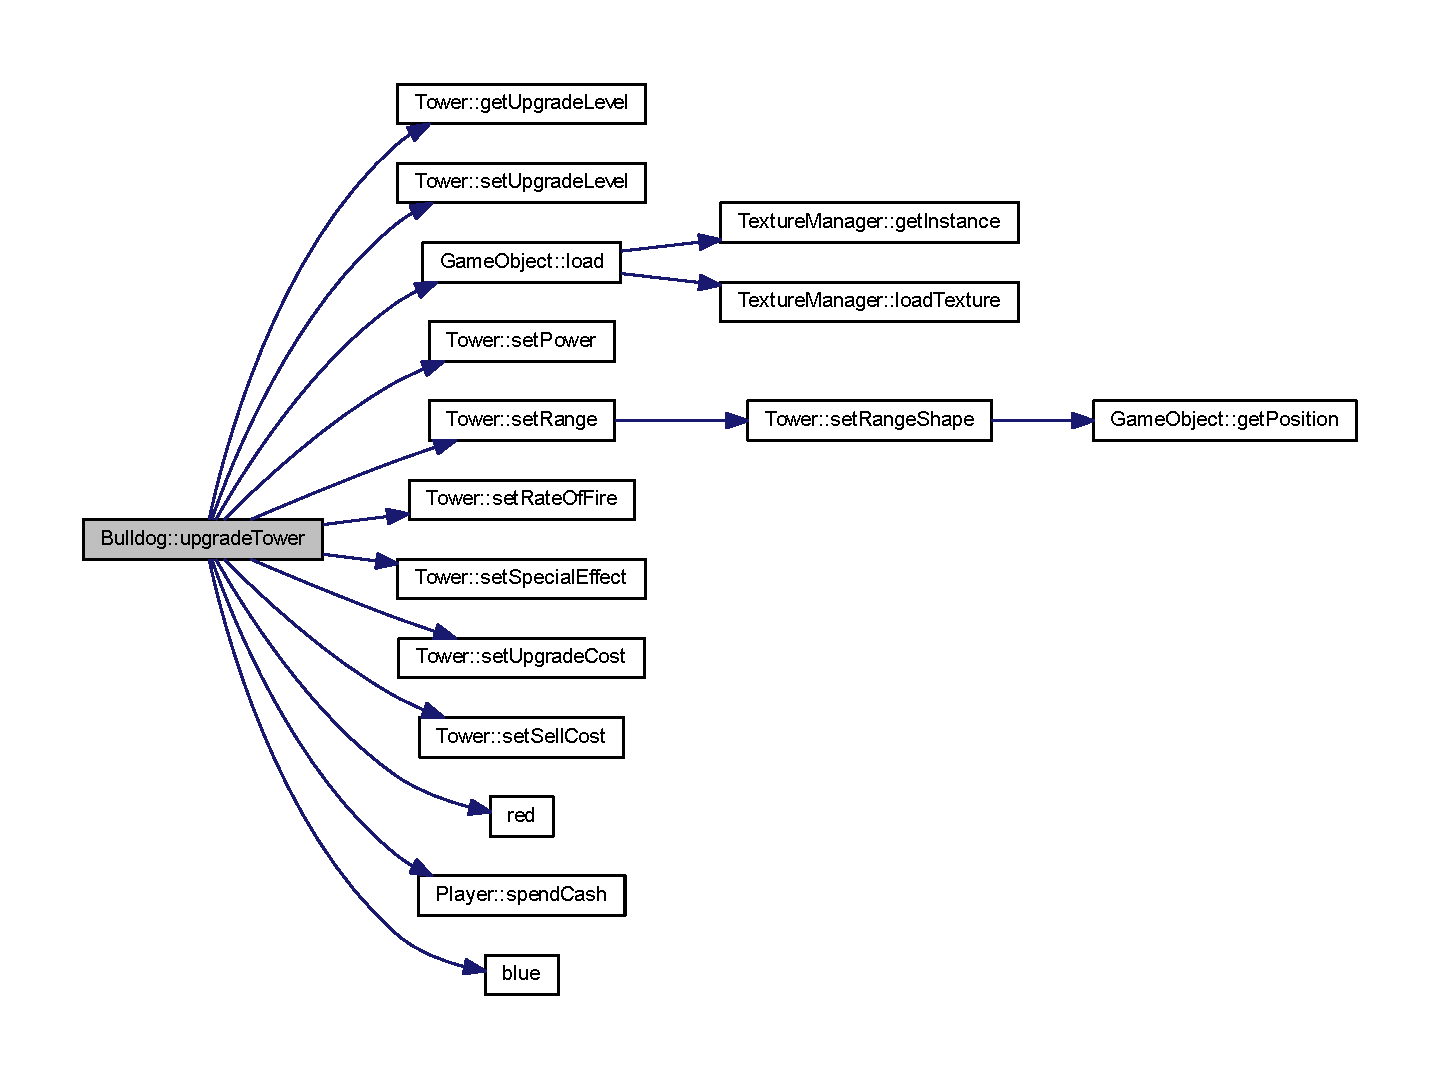
\includegraphics[width=350pt]{class_bulldog_adfecd22f881be0d7946534c2012275d7_cgraph}
\end{center}
\end{figure}




The documentation for this class was generated from the following files\+:\begin{DoxyCompactItemize}
\item 
jamms/\+Tower\+Defense/\+Tower\+Defense/include/game\+Objects/\hyperlink{_bulldog_8h}{Bulldog.\+h}\item 
jamms/\+Tower\+Defense/\+Tower\+Defense/src/game\+Objects/\hyperlink{_bulldog_8cpp}{Bulldog.\+cpp}\end{DoxyCompactItemize}

\hypertarget{structcolor}{\section{color Struct Reference}
\label{structcolor}\index{color@{color}}
}


{\ttfamily \#include $<$Console\+Color.\+h$>$}



Collaboration diagram for color\+:
\nopagebreak
\begin{figure}[H]
\begin{center}
\leavevmode
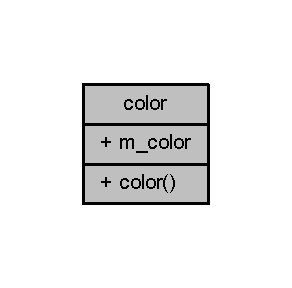
\includegraphics[width=140pt]{structcolor__coll__graph}
\end{center}
\end{figure}
\subsection*{Public Member Functions}
\begin{DoxyCompactItemize}
\item 
\hyperlink{structcolor_a691c0cd0bd4daa4674d2f7ef901c9c6c}{color} (W\+O\+R\+D attribute)
\end{DoxyCompactItemize}
\subsection*{Public Attributes}
\begin{DoxyCompactItemize}
\item 
W\+O\+R\+D \hyperlink{structcolor_a899a29a2834627301d67fd52ed970043}{m\+\_\+color}
\end{DoxyCompactItemize}


\subsection{Constructor \& Destructor Documentation}
\hypertarget{structcolor_a691c0cd0bd4daa4674d2f7ef901c9c6c}{\index{color@{color}!color@{color}}
\index{color@{color}!color@{color}}
\subsubsection[{color}]{\setlength{\rightskip}{0pt plus 5cm}color\+::color (
\begin{DoxyParamCaption}
\item[{W\+O\+R\+D}]{attribute}
\end{DoxyParamCaption}
)\hspace{0.3cm}{\ttfamily [inline]}}}\label{structcolor_a691c0cd0bd4daa4674d2f7ef901c9c6c}


\subsection{Member Data Documentation}
\hypertarget{structcolor_a899a29a2834627301d67fd52ed970043}{\index{color@{color}!m\+\_\+color@{m\+\_\+color}}
\index{m\+\_\+color@{m\+\_\+color}!color@{color}}
\subsubsection[{m\+\_\+color}]{\setlength{\rightskip}{0pt plus 5cm}W\+O\+R\+D color\+::m\+\_\+color}}\label{structcolor_a899a29a2834627301d67fd52ed970043}


The documentation for this struct was generated from the following file\+:\begin{DoxyCompactItemize}
\item 
jamms/\+Tower\+Defense/\+Tower\+Defense/include/utils/\hyperlink{_console_color_8h}{Console\+Color.\+h}\end{DoxyCompactItemize}

\hypertarget{class_critter}{\section{Critter Class Reference}
\label{class_critter}\index{Critter@{Critter}}
}


Abstract base class of all Critters \hyperlink{class_critter}{Critter} defines the attributes, accessors, and update function for its subclass instances.  




{\ttfamily \#include $<$Critter.\+h$>$}



Inheritance diagram for Critter\+:
\nopagebreak
\begin{figure}[H]
\begin{center}
\leavevmode
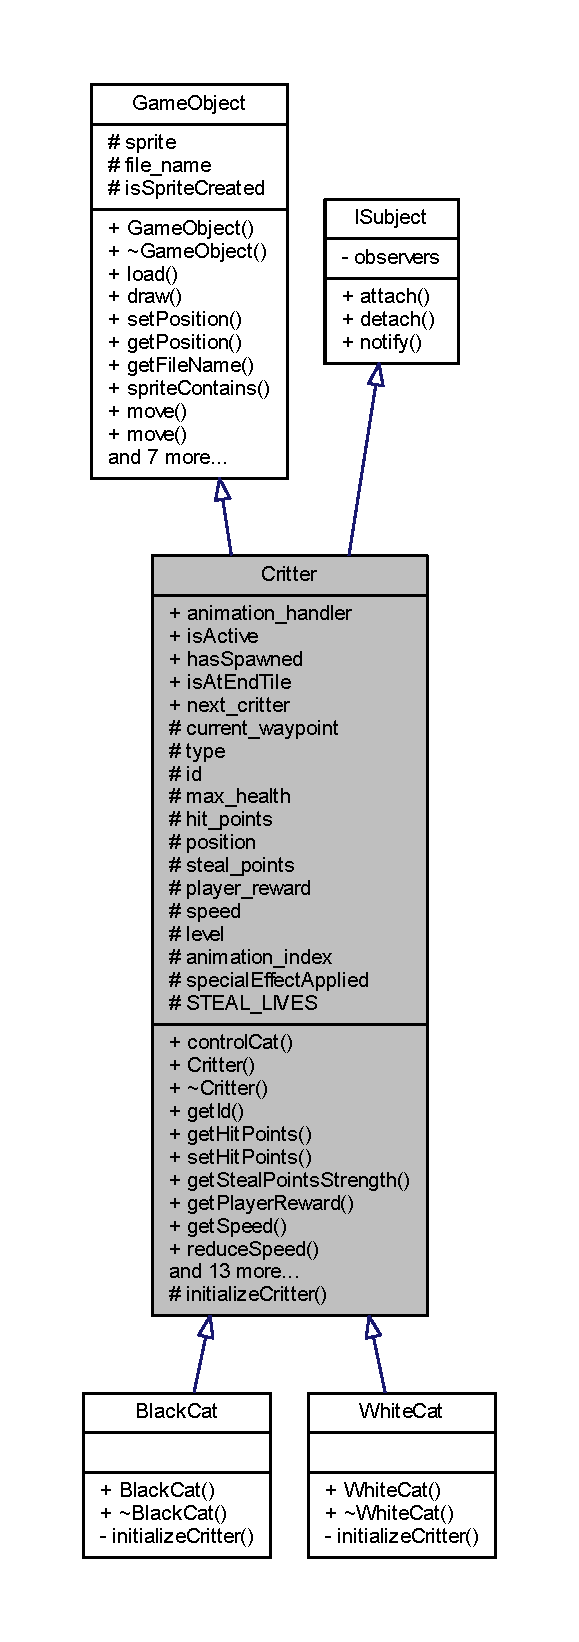
\includegraphics[height=550pt]{class_critter__inherit__graph}
\end{center}
\end{figure}


Collaboration diagram for Critter\+:
\nopagebreak
\begin{figure}[H]
\begin{center}
\leavevmode
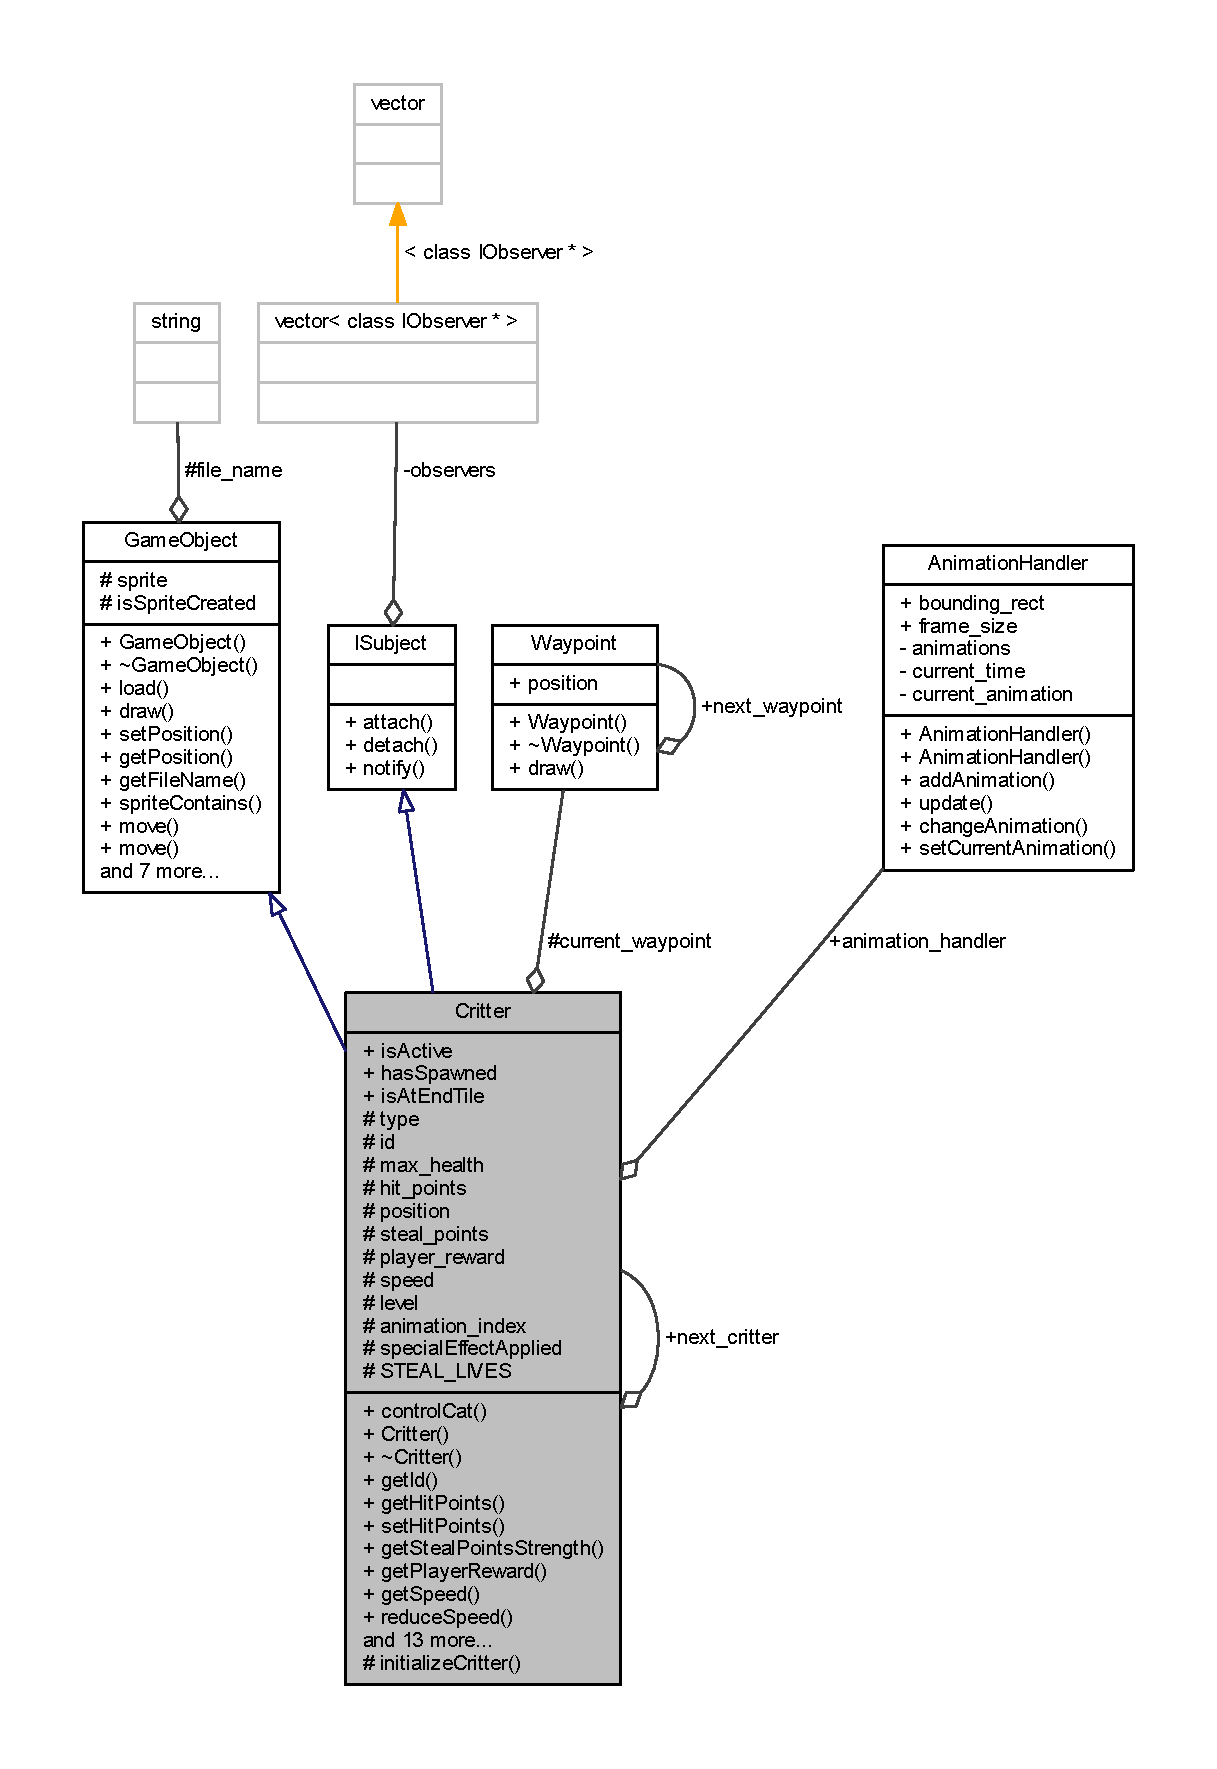
\includegraphics[height=550pt]{class_critter__coll__graph}
\end{center}
\end{figure}
\subsection*{Public Types}
\begin{DoxyCompactItemize}
\item 
enum \hyperlink{class_critter_acda8a5c3234b66101e0546d75d6f90f1}{Critter\+Type} \{ \hyperlink{class_critter_acda8a5c3234b66101e0546d75d6f90f1a91135fa8da5b64a8a556e8c198b46fe9}{B\+L\+A\+C\+K\+\_\+\+C\+A\+T}, 
\hyperlink{class_critter_acda8a5c3234b66101e0546d75d6f90f1ac88c727edcec187617ee3707d2c193c5}{W\+H\+I\+T\+E\+\_\+\+C\+A\+T}
 \}
\end{DoxyCompactItemize}
\subsection*{Public Member Functions}
\begin{DoxyCompactItemize}
\item 
\hyperlink{class_critter_a05aa21e3b570d7380f3ead47c99442ef}{Critter} ()
\item 
virtual \hyperlink{class_critter_a23e65a0917fc76bcf349e2a28fad5c42}{$\sim$\+Critter} ()
\item 
int \hyperlink{class_critter_a5636f0ed2f067318e0d361fe31c9eff2}{get\+Id} () const 
\item 
int \hyperlink{class_critter_a1e98c05f5a41102cc37eb7a4396b90cf}{get\+Hit\+Points} () const 
\item 
void \hyperlink{class_critter_adca76b21049a0bdd0b3e1505996c71ea}{set\+Hit\+Points} (int points)
\item 
int \hyperlink{class_critter_ac57f38074517fa1cc481380aaff1ed85}{get\+Steal\+Points\+Strength} () const 
\item 
int \hyperlink{class_critter_a7db2281b14479a1c931716c07acbc7da}{get\+Player\+Reward} () const 
\item 
float \hyperlink{class_critter_a3785ffa05cec86b30264fbdbf613e4f8}{get\+Speed} () const 
\item 
void \hyperlink{class_critter_a52be1f776c5c8fbcba1efadceaccc759}{set\+Speed} (float \hyperlink{class_critter_adde7d84a0dd9ac8f5dc144464928638f}{speed})
\item 
void \hyperlink{class_critter_ae843395fb1106cd2c550cd9be9f14df0}{reduce\+Speed} (float \hyperlink{class_critter_adde7d84a0dd9ac8f5dc144464928638f}{speed})
\item 
int \hyperlink{class_critter_aebbb372bdcd3a709428445554c3d24c9}{get\+Level} () const 
\item 
bool \hyperlink{class_critter_aaf084b7cd4ffaa632454ee363723db92}{get\+Special\+Effect\+Applied} () const 
\item 
void \hyperlink{class_critter_a662c3e493cd09b78df86afdc3c0725df}{set\+Special\+Effect\+Applied} (bool \hyperlink{class_critter_aa30e57414bd64c920dca286f87da5c3f}{special\+Effect\+Applied})
\item 
void \hyperlink{class_critter_a3601e12d79247c3345e9e828688cf321}{inflict\+Damage} (int dmg)
\item 
std\+::string \hyperlink{class_critter_ae0799b0a4602623632fa382e5ad0d0c8}{get\+Critter\+Specs} ()
\item 
void \hyperlink{class_critter_a50549d8f01246886b931345865ec9949}{add\+Effect} (\hyperlink{class_critter_effect}{Critter\+Effect} $\ast$effect)
\item 
void \hyperlink{class_critter_a06a644a7f12cde7d40679b396c4a3796}{inflict\+Effects} ()
\end{DoxyCompactItemize}
\subsection*{Public Attributes}
\begin{DoxyCompactItemize}
\item 
\hyperlink{class_critter}{Critter} $\ast$ \hyperlink{class_critter_a6017fbb8c863a2456f43b88996720927}{next\+\_\+critter}
\end{DoxyCompactItemize}
\subsection*{Protected Member Functions}
\begin{DoxyCompactItemize}
\item 
virtual void \hyperlink{class_critter_ad425da71f01445ee175e5f98d94ca0ba}{initialize\+Critter} (const std\+::vector$<$ \hyperlink{class_animation}{Animation} $>$ \&animations)=0
\begin{DoxyCompactList}\small\item\em Pure virtualized initialization function for \hyperlink{class_critter}{Critter}. \end{DoxyCompactList}\end{DoxyCompactItemize}
\subsection*{Protected Attributes}
\begin{DoxyCompactItemize}
\item 
\hyperlink{class_critter_acda8a5c3234b66101e0546d75d6f90f1}{Critter\+Type} \hyperlink{class_critter_ac59fc8262aaffbdae6f2823460b58737}{type}
\item 
int \hyperlink{class_critter_ae775e0ebe6e8bbe249c403670bda46f8}{id}
\item 
int \hyperlink{class_critter_a9b2e317fb3a104ea9b449f77c81d7d7a}{max\+\_\+health}
\item 
std\+::list$<$ std\+::unique\+\_\+ptr\\*
$<$ \hyperlink{class_critter_effect}{Critter\+Effect} $>$ $>$ \hyperlink{class_critter_a9974fdc5dd5ef5afc8ff2fffbd2261e0}{effect\+List}
\item 
int \hyperlink{class_critter_a916038a11e8443ea403a644e91fc791e}{hit\+\_\+points}
\begin{DoxyCompactList}\small\item\em Health of the \hyperlink{class_critter}{Critter}. \end{DoxyCompactList}\item 
int \hyperlink{class_critter_ad2b5b3ee8a0b69d4023f60cfb9f26a6a}{steal\+\_\+points}
\begin{DoxyCompactList}\small\item\em Rate at which the critter can steal points from the player. \end{DoxyCompactList}\item 
int \hyperlink{class_critter_a2a17f7366fbde83714742e66ba3e63a7}{player\+\_\+reward}
\begin{DoxyCompactList}\small\item\em Coin reward for the player when the \hyperlink{class_critter}{Critter} is killed. \end{DoxyCompactList}\item 
float \hyperlink{class_critter_adde7d84a0dd9ac8f5dc144464928638f}{speed}
\begin{DoxyCompactList}\small\item\em \hyperlink{class_critter}{Critter} movement speed. \end{DoxyCompactList}\item 
float \hyperlink{class_critter_ad53189c28d3f392ea8d1f1796e7c0744}{speed\+Modifier}
\item 
int \hyperlink{class_critter_a9f9a6408a55212036f317710dc3da410}{level}
\begin{DoxyCompactList}\small\item\em Difficulty level as part of a wave. \end{DoxyCompactList}\item 
bool \hyperlink{class_critter_aa30e57414bd64c920dca286f87da5c3f}{special\+Effect\+Applied}
\end{DoxyCompactItemize}
\subsection*{Static Protected Attributes}
\begin{DoxyCompactItemize}
\item 
static const int \hyperlink{class_critter_a1324eb838f1790e904a0b82c9ceed173}{S\+T\+E\+A\+L\+\_\+\+L\+I\+V\+E\+S} = 1
\begin{DoxyCompactList}\small\item\em Rate at which the critter can steal lives from the player. \end{DoxyCompactList}\end{DoxyCompactItemize}


\subsection{Detailed Description}
Abstract base class of all Critters \hyperlink{class_critter}{Critter} defines the attributes, accessors, and update function for its subclass instances. 

\subsection{Member Enumeration Documentation}
\hypertarget{class_critter_acda8a5c3234b66101e0546d75d6f90f1}{\index{Critter@{Critter}!Critter\+Type@{Critter\+Type}}
\index{Critter\+Type@{Critter\+Type}!Critter@{Critter}}
\subsubsection[{Critter\+Type}]{\setlength{\rightskip}{0pt plus 5cm}enum {\bf Critter\+::\+Critter\+Type}}}\label{class_critter_acda8a5c3234b66101e0546d75d6f90f1}
\begin{Desc}
\item[Enumerator]\par
\begin{description}
\index{B\+L\+A\+C\+K\+\_\+\+C\+A\+T@{B\+L\+A\+C\+K\+\_\+\+C\+A\+T}!Critter@{Critter}}\index{Critter@{Critter}!B\+L\+A\+C\+K\+\_\+\+C\+A\+T@{B\+L\+A\+C\+K\+\_\+\+C\+A\+T}}\item[{\em 
\hypertarget{class_critter_acda8a5c3234b66101e0546d75d6f90f1a91135fa8da5b64a8a556e8c198b46fe9}{B\+L\+A\+C\+K\+\_\+\+C\+A\+T}\label{class_critter_acda8a5c3234b66101e0546d75d6f90f1a91135fa8da5b64a8a556e8c198b46fe9}
}]\index{W\+H\+I\+T\+E\+\_\+\+C\+A\+T@{W\+H\+I\+T\+E\+\_\+\+C\+A\+T}!Critter@{Critter}}\index{Critter@{Critter}!W\+H\+I\+T\+E\+\_\+\+C\+A\+T@{W\+H\+I\+T\+E\+\_\+\+C\+A\+T}}\item[{\em 
\hypertarget{class_critter_acda8a5c3234b66101e0546d75d6f90f1ac88c727edcec187617ee3707d2c193c5}{W\+H\+I\+T\+E\+\_\+\+C\+A\+T}\label{class_critter_acda8a5c3234b66101e0546d75d6f90f1ac88c727edcec187617ee3707d2c193c5}
}]\end{description}
\end{Desc}


\subsection{Constructor \& Destructor Documentation}
\hypertarget{class_critter_a05aa21e3b570d7380f3ead47c99442ef}{\index{Critter@{Critter}!Critter@{Critter}}
\index{Critter@{Critter}!Critter@{Critter}}
\subsubsection[{Critter}]{\setlength{\rightskip}{0pt plus 5cm}Critter\+::\+Critter (
\begin{DoxyParamCaption}
{}
\end{DoxyParamCaption}
)}}\label{class_critter_a05aa21e3b570d7380f3ead47c99442ef}
\hypertarget{class_critter_a23e65a0917fc76bcf349e2a28fad5c42}{\index{Critter@{Critter}!````~Critter@{$\sim$\+Critter}}
\index{````~Critter@{$\sim$\+Critter}!Critter@{Critter}}
\subsubsection[{$\sim$\+Critter}]{\setlength{\rightskip}{0pt plus 5cm}Critter\+::$\sim$\+Critter (
\begin{DoxyParamCaption}
{}
\end{DoxyParamCaption}
)\hspace{0.3cm}{\ttfamily [virtual]}}}\label{class_critter_a23e65a0917fc76bcf349e2a28fad5c42}


\subsection{Member Function Documentation}
\hypertarget{class_critter_a50549d8f01246886b931345865ec9949}{\index{Critter@{Critter}!add\+Effect@{add\+Effect}}
\index{add\+Effect@{add\+Effect}!Critter@{Critter}}
\subsubsection[{add\+Effect}]{\setlength{\rightskip}{0pt plus 5cm}void Critter\+::add\+Effect (
\begin{DoxyParamCaption}
\item[{{\bf Critter\+Effect} $\ast$}]{effect}
\end{DoxyParamCaption}
)}}\label{class_critter_a50549d8f01246886b931345865ec9949}


Here is the call graph for this function\+:
\nopagebreak
\begin{figure}[H]
\begin{center}
\leavevmode
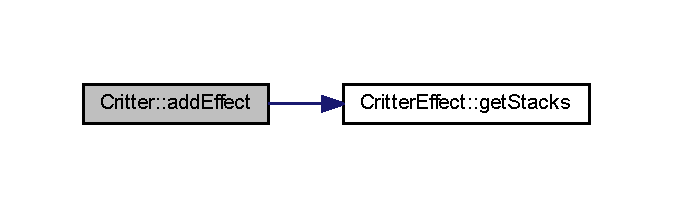
\includegraphics[width=323pt]{class_critter_a50549d8f01246886b931345865ec9949_cgraph}
\end{center}
\end{figure}




Here is the caller graph for this function\+:
\nopagebreak
\begin{figure}[H]
\begin{center}
\leavevmode
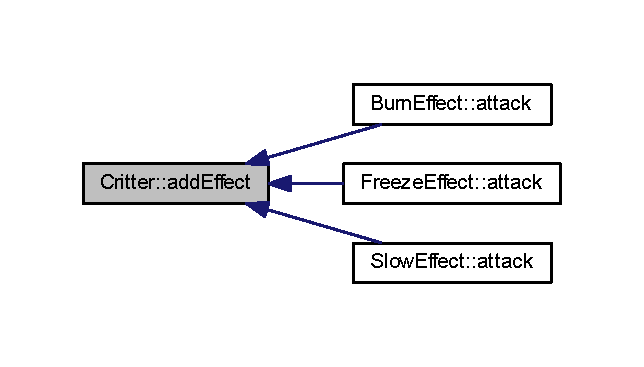
\includegraphics[width=309pt]{class_critter_a50549d8f01246886b931345865ec9949_icgraph}
\end{center}
\end{figure}


\hypertarget{class_critter_ae0799b0a4602623632fa382e5ad0d0c8}{\index{Critter@{Critter}!get\+Critter\+Specs@{get\+Critter\+Specs}}
\index{get\+Critter\+Specs@{get\+Critter\+Specs}!Critter@{Critter}}
\subsubsection[{get\+Critter\+Specs}]{\setlength{\rightskip}{0pt plus 5cm}std\+::string Critter\+::get\+Critter\+Specs (
\begin{DoxyParamCaption}
{}
\end{DoxyParamCaption}
)}}\label{class_critter_ae0799b0a4602623632fa382e5ad0d0c8}


Here is the call graph for this function\+:
\nopagebreak
\begin{figure}[H]
\begin{center}
\leavevmode
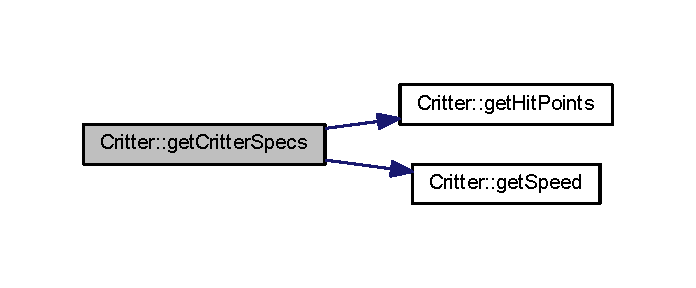
\includegraphics[width=334pt]{class_critter_ae0799b0a4602623632fa382e5ad0d0c8_cgraph}
\end{center}
\end{figure}




Here is the caller graph for this function\+:\nopagebreak
\begin{figure}[H]
\begin{center}
\leavevmode
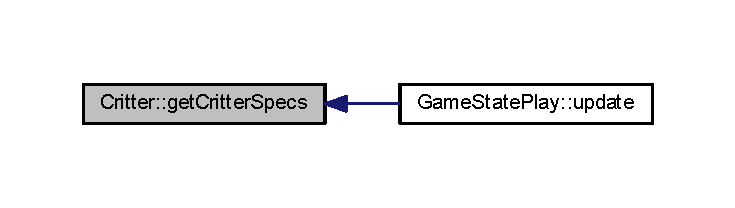
\includegraphics[width=350pt]{class_critter_ae0799b0a4602623632fa382e5ad0d0c8_icgraph}
\end{center}
\end{figure}


\hypertarget{class_critter_a1e98c05f5a41102cc37eb7a4396b90cf}{\index{Critter@{Critter}!get\+Hit\+Points@{get\+Hit\+Points}}
\index{get\+Hit\+Points@{get\+Hit\+Points}!Critter@{Critter}}
\subsubsection[{get\+Hit\+Points}]{\setlength{\rightskip}{0pt plus 5cm}int Critter\+::get\+Hit\+Points (
\begin{DoxyParamCaption}
{}
\end{DoxyParamCaption}
) const}}\label{class_critter_a1e98c05f5a41102cc37eb7a4396b90cf}


Here is the caller graph for this function\+:
\nopagebreak
\begin{figure}[H]
\begin{center}
\leavevmode
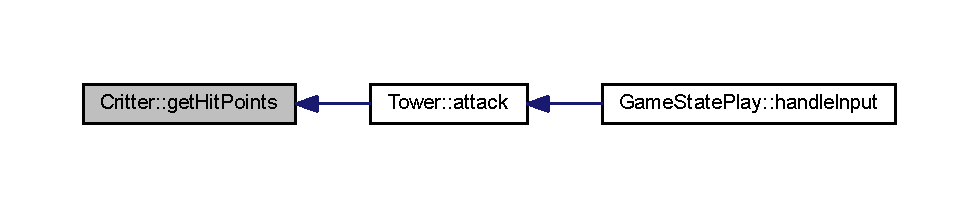
\includegraphics[width=350pt]{class_critter_a1e98c05f5a41102cc37eb7a4396b90cf_icgraph}
\end{center}
\end{figure}


\hypertarget{class_critter_a5636f0ed2f067318e0d361fe31c9eff2}{\index{Critter@{Critter}!get\+Id@{get\+Id}}
\index{get\+Id@{get\+Id}!Critter@{Critter}}
\subsubsection[{get\+Id}]{\setlength{\rightskip}{0pt plus 5cm}int Critter\+::get\+Id (
\begin{DoxyParamCaption}
{}
\end{DoxyParamCaption}
) const}}\label{class_critter_a5636f0ed2f067318e0d361fe31c9eff2}


Here is the caller graph for this function\+:
\nopagebreak
\begin{figure}[H]
\begin{center}
\leavevmode
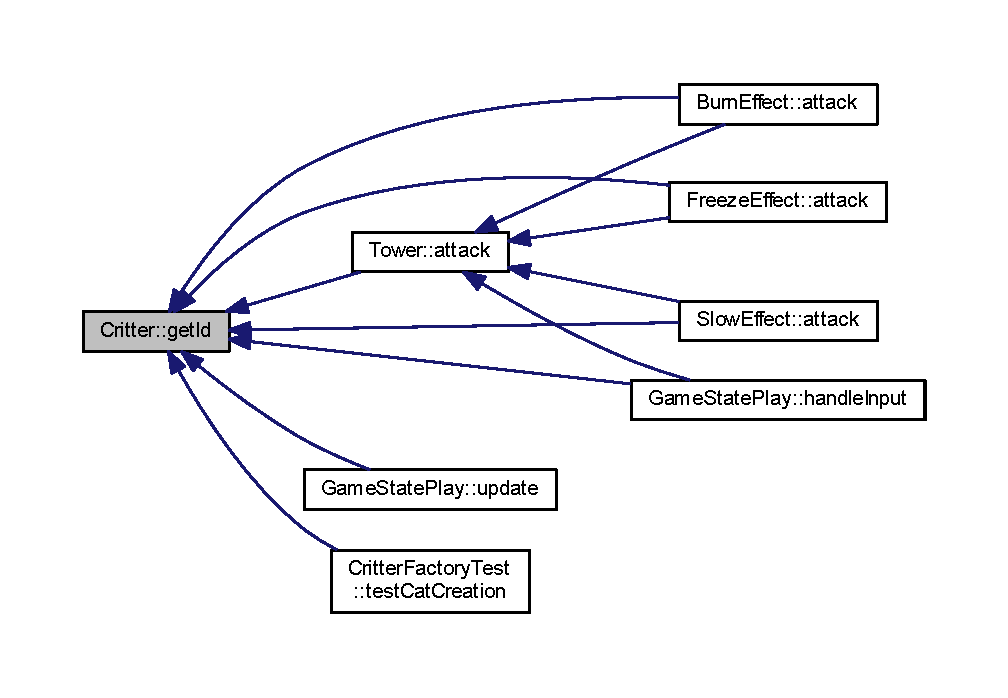
\includegraphics[width=350pt]{class_critter_a5636f0ed2f067318e0d361fe31c9eff2_icgraph}
\end{center}
\end{figure}


\hypertarget{class_critter_aebbb372bdcd3a709428445554c3d24c9}{\index{Critter@{Critter}!get\+Level@{get\+Level}}
\index{get\+Level@{get\+Level}!Critter@{Critter}}
\subsubsection[{get\+Level}]{\setlength{\rightskip}{0pt plus 5cm}int Critter\+::get\+Level (
\begin{DoxyParamCaption}
{}
\end{DoxyParamCaption}
) const}}\label{class_critter_aebbb372bdcd3a709428445554c3d24c9}
\hypertarget{class_critter_a7db2281b14479a1c931716c07acbc7da}{\index{Critter@{Critter}!get\+Player\+Reward@{get\+Player\+Reward}}
\index{get\+Player\+Reward@{get\+Player\+Reward}!Critter@{Critter}}
\subsubsection[{get\+Player\+Reward}]{\setlength{\rightskip}{0pt plus 5cm}int Critter\+::get\+Player\+Reward (
\begin{DoxyParamCaption}
{}
\end{DoxyParamCaption}
) const}}\label{class_critter_a7db2281b14479a1c931716c07acbc7da}


Here is the caller graph for this function\+:
\nopagebreak
\begin{figure}[H]
\begin{center}
\leavevmode
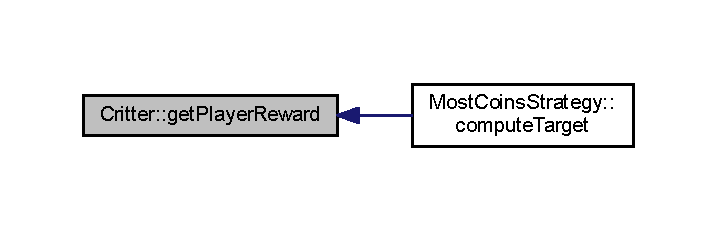
\includegraphics[width=344pt]{class_critter_a7db2281b14479a1c931716c07acbc7da_icgraph}
\end{center}
\end{figure}


\hypertarget{class_critter_aaf084b7cd4ffaa632454ee363723db92}{\index{Critter@{Critter}!get\+Special\+Effect\+Applied@{get\+Special\+Effect\+Applied}}
\index{get\+Special\+Effect\+Applied@{get\+Special\+Effect\+Applied}!Critter@{Critter}}
\subsubsection[{get\+Special\+Effect\+Applied}]{\setlength{\rightskip}{0pt plus 5cm}bool Critter\+::get\+Special\+Effect\+Applied (
\begin{DoxyParamCaption}
{}
\end{DoxyParamCaption}
) const}}\label{class_critter_aaf084b7cd4ffaa632454ee363723db92}
\hypertarget{class_critter_a3785ffa05cec86b30264fbdbf613e4f8}{\index{Critter@{Critter}!get\+Speed@{get\+Speed}}
\index{get\+Speed@{get\+Speed}!Critter@{Critter}}
\subsubsection[{get\+Speed}]{\setlength{\rightskip}{0pt plus 5cm}float Critter\+::get\+Speed (
\begin{DoxyParamCaption}
{}
\end{DoxyParamCaption}
) const}}\label{class_critter_a3785ffa05cec86b30264fbdbf613e4f8}


Here is the caller graph for this function\+:
\nopagebreak
\begin{figure}[H]
\begin{center}
\leavevmode
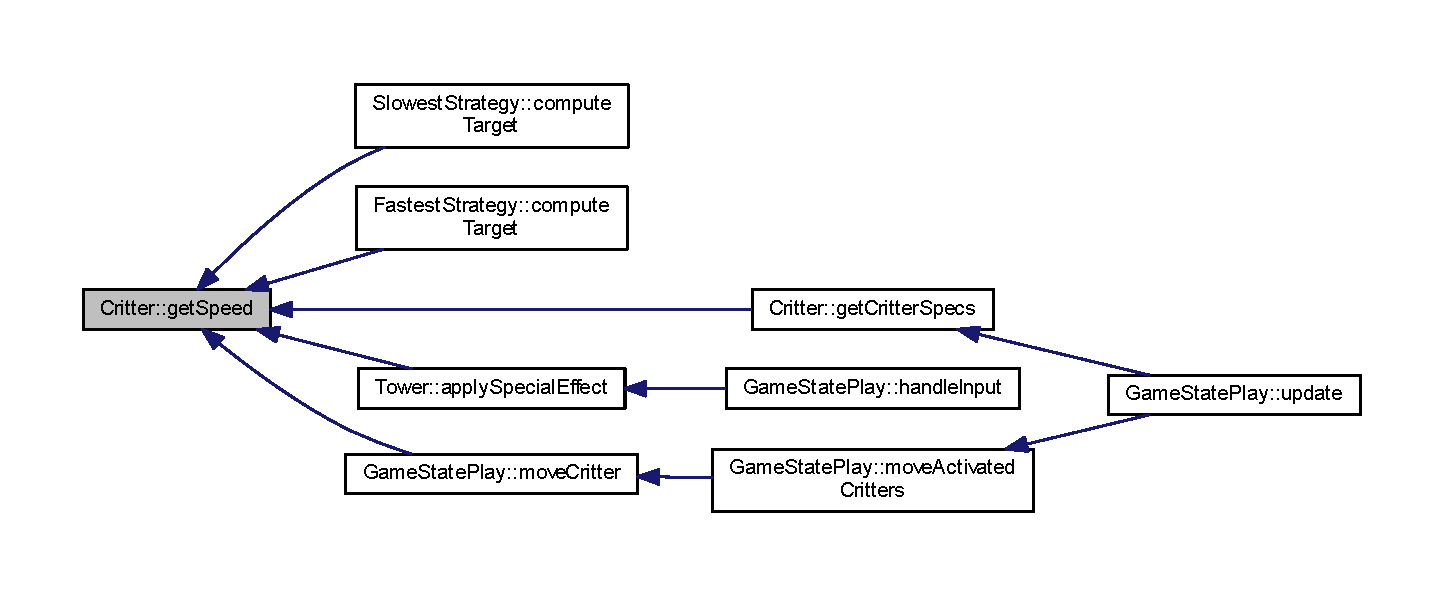
\includegraphics[width=350pt]{class_critter_a3785ffa05cec86b30264fbdbf613e4f8_icgraph}
\end{center}
\end{figure}


\hypertarget{class_critter_ac57f38074517fa1cc481380aaff1ed85}{\index{Critter@{Critter}!get\+Steal\+Points\+Strength@{get\+Steal\+Points\+Strength}}
\index{get\+Steal\+Points\+Strength@{get\+Steal\+Points\+Strength}!Critter@{Critter}}
\subsubsection[{get\+Steal\+Points\+Strength}]{\setlength{\rightskip}{0pt plus 5cm}int Critter\+::get\+Steal\+Points\+Strength (
\begin{DoxyParamCaption}
{}
\end{DoxyParamCaption}
) const}}\label{class_critter_ac57f38074517fa1cc481380aaff1ed85}


Here is the caller graph for this function\+:
\nopagebreak
\begin{figure}[H]
\begin{center}
\leavevmode
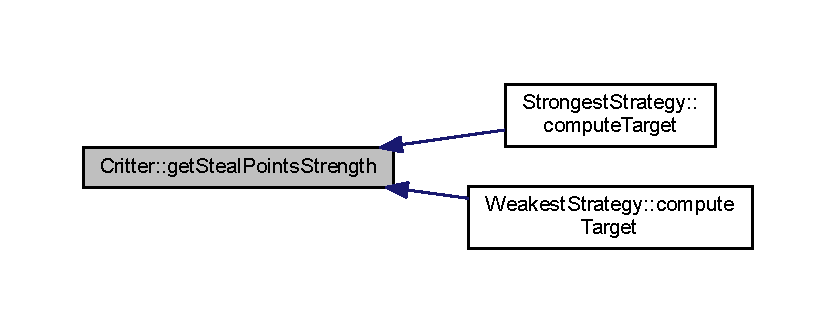
\includegraphics[width=350pt]{class_critter_ac57f38074517fa1cc481380aaff1ed85_icgraph}
\end{center}
\end{figure}


\hypertarget{class_critter_a3601e12d79247c3345e9e828688cf321}{\index{Critter@{Critter}!inflict\+Damage@{inflict\+Damage}}
\index{inflict\+Damage@{inflict\+Damage}!Critter@{Critter}}
\subsubsection[{inflict\+Damage}]{\setlength{\rightskip}{0pt plus 5cm}void Critter\+::inflict\+Damage (
\begin{DoxyParamCaption}
\item[{int}]{dmg}
\end{DoxyParamCaption}
)}}\label{class_critter_a3601e12d79247c3345e9e828688cf321}


Here is the caller graph for this function\+:
\nopagebreak
\begin{figure}[H]
\begin{center}
\leavevmode
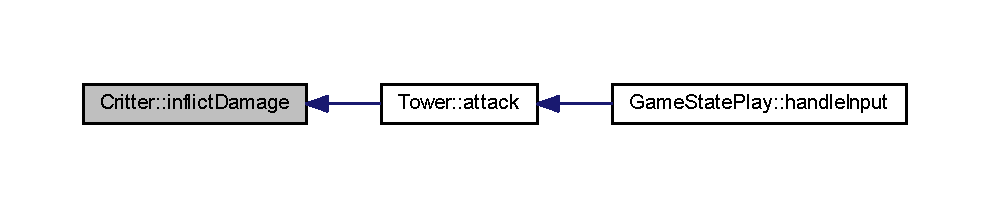
\includegraphics[width=350pt]{class_critter_a3601e12d79247c3345e9e828688cf321_icgraph}
\end{center}
\end{figure}


\hypertarget{class_critter_a06a644a7f12cde7d40679b396c4a3796}{\index{Critter@{Critter}!inflict\+Effects@{inflict\+Effects}}
\index{inflict\+Effects@{inflict\+Effects}!Critter@{Critter}}
\subsubsection[{inflict\+Effects}]{\setlength{\rightskip}{0pt plus 5cm}void Critter\+::inflict\+Effects (
\begin{DoxyParamCaption}
{}
\end{DoxyParamCaption}
)}}\label{class_critter_a06a644a7f12cde7d40679b396c4a3796}


Here is the call graph for this function\+:
\nopagebreak
\begin{figure}[H]
\begin{center}
\leavevmode
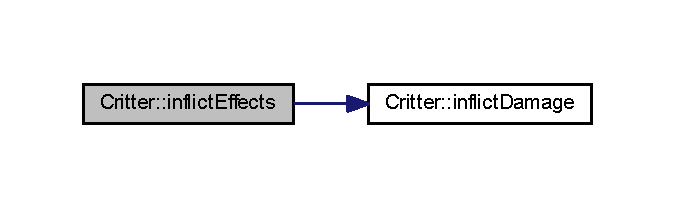
\includegraphics[width=324pt]{class_critter_a06a644a7f12cde7d40679b396c4a3796_cgraph}
\end{center}
\end{figure}


\hypertarget{class_critter_ad425da71f01445ee175e5f98d94ca0ba}{\index{Critter@{Critter}!initialize\+Critter@{initialize\+Critter}}
\index{initialize\+Critter@{initialize\+Critter}!Critter@{Critter}}
\subsubsection[{initialize\+Critter}]{\setlength{\rightskip}{0pt plus 5cm}virtual void Critter\+::initialize\+Critter (
\begin{DoxyParamCaption}
\item[{const std\+::vector$<$ {\bf Animation} $>$ \&}]{animations}
\end{DoxyParamCaption}
)\hspace{0.3cm}{\ttfamily [protected]}, {\ttfamily [pure virtual]}}}\label{class_critter_ad425da71f01445ee175e5f98d94ca0ba}


Pure virtualized initialization function for \hyperlink{class_critter}{Critter}. 

\begin{DoxyReturn}{Returns}
Void. 
\end{DoxyReturn}


Implemented in \hyperlink{class_black_cat_a2ae946e05f754f7d7bdbc753946425eb}{Black\+Cat}, and \hyperlink{class_white_cat_a0a3c801e7a6b451b2b1caef9da137585}{White\+Cat}.

\hypertarget{class_critter_ae843395fb1106cd2c550cd9be9f14df0}{\index{Critter@{Critter}!reduce\+Speed@{reduce\+Speed}}
\index{reduce\+Speed@{reduce\+Speed}!Critter@{Critter}}
\subsubsection[{reduce\+Speed}]{\setlength{\rightskip}{0pt plus 5cm}void Critter\+::reduce\+Speed (
\begin{DoxyParamCaption}
\item[{float}]{speed}
\end{DoxyParamCaption}
)}}\label{class_critter_ae843395fb1106cd2c550cd9be9f14df0}


Here is the caller graph for this function\+:\nopagebreak
\begin{figure}[H]
\begin{center}
\leavevmode
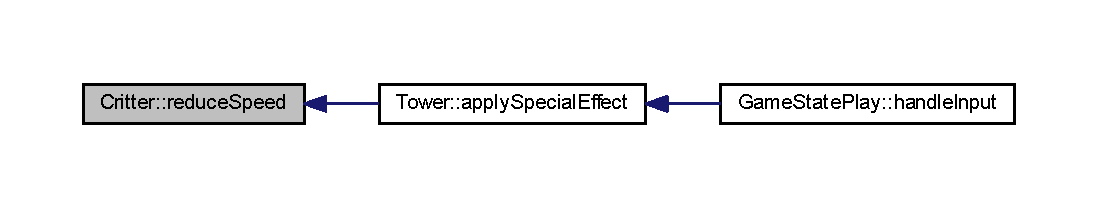
\includegraphics[width=350pt]{class_critter_ae843395fb1106cd2c550cd9be9f14df0_icgraph}
\end{center}
\end{figure}


\hypertarget{class_critter_adca76b21049a0bdd0b3e1505996c71ea}{\index{Critter@{Critter}!set\+Hit\+Points@{set\+Hit\+Points}}
\index{set\+Hit\+Points@{set\+Hit\+Points}!Critter@{Critter}}
\subsubsection[{set\+Hit\+Points}]{\setlength{\rightskip}{0pt plus 5cm}void Critter\+::set\+Hit\+Points (
\begin{DoxyParamCaption}
\item[{int}]{points}
\end{DoxyParamCaption}
)}}\label{class_critter_adca76b21049a0bdd0b3e1505996c71ea}
\hypertarget{class_critter_a662c3e493cd09b78df86afdc3c0725df}{\index{Critter@{Critter}!set\+Special\+Effect\+Applied@{set\+Special\+Effect\+Applied}}
\index{set\+Special\+Effect\+Applied@{set\+Special\+Effect\+Applied}!Critter@{Critter}}
\subsubsection[{set\+Special\+Effect\+Applied}]{\setlength{\rightskip}{0pt plus 5cm}void Critter\+::set\+Special\+Effect\+Applied (
\begin{DoxyParamCaption}
\item[{bool}]{special\+Effect\+Applied}
\end{DoxyParamCaption}
)}}\label{class_critter_a662c3e493cd09b78df86afdc3c0725df}
\hypertarget{class_critter_a52be1f776c5c8fbcba1efadceaccc759}{\index{Critter@{Critter}!set\+Speed@{set\+Speed}}
\index{set\+Speed@{set\+Speed}!Critter@{Critter}}
\subsubsection[{set\+Speed}]{\setlength{\rightskip}{0pt plus 5cm}void Critter\+::set\+Speed (
\begin{DoxyParamCaption}
\item[{float}]{speed}
\end{DoxyParamCaption}
)}}\label{class_critter_a52be1f776c5c8fbcba1efadceaccc759}


\subsection{Member Data Documentation}
\hypertarget{class_critter_a9974fdc5dd5ef5afc8ff2fffbd2261e0}{\index{Critter@{Critter}!effect\+List@{effect\+List}}
\index{effect\+List@{effect\+List}!Critter@{Critter}}
\subsubsection[{effect\+List}]{\setlength{\rightskip}{0pt plus 5cm}std\+::list$<$std\+::unique\+\_\+ptr$<${\bf Critter\+Effect}$>$ $>$ Critter\+::effect\+List\hspace{0.3cm}{\ttfamily [protected]}}}\label{class_critter_a9974fdc5dd5ef5afc8ff2fffbd2261e0}
\hypertarget{class_critter_a916038a11e8443ea403a644e91fc791e}{\index{Critter@{Critter}!hit\+\_\+points@{hit\+\_\+points}}
\index{hit\+\_\+points@{hit\+\_\+points}!Critter@{Critter}}
\subsubsection[{hit\+\_\+points}]{\setlength{\rightskip}{0pt plus 5cm}int Critter\+::hit\+\_\+points\hspace{0.3cm}{\ttfamily [protected]}}}\label{class_critter_a916038a11e8443ea403a644e91fc791e}


Health of the \hyperlink{class_critter}{Critter}. 

\hypertarget{class_critter_ae775e0ebe6e8bbe249c403670bda46f8}{\index{Critter@{Critter}!id@{id}}
\index{id@{id}!Critter@{Critter}}
\subsubsection[{id}]{\setlength{\rightskip}{0pt plus 5cm}int Critter\+::id\hspace{0.3cm}{\ttfamily [protected]}}}\label{class_critter_ae775e0ebe6e8bbe249c403670bda46f8}
\hypertarget{class_critter_a9f9a6408a55212036f317710dc3da410}{\index{Critter@{Critter}!level@{level}}
\index{level@{level}!Critter@{Critter}}
\subsubsection[{level}]{\setlength{\rightskip}{0pt plus 5cm}int Critter\+::level\hspace{0.3cm}{\ttfamily [protected]}}}\label{class_critter_a9f9a6408a55212036f317710dc3da410}


Difficulty level as part of a wave. 

\hypertarget{class_critter_a9b2e317fb3a104ea9b449f77c81d7d7a}{\index{Critter@{Critter}!max\+\_\+health@{max\+\_\+health}}
\index{max\+\_\+health@{max\+\_\+health}!Critter@{Critter}}
\subsubsection[{max\+\_\+health}]{\setlength{\rightskip}{0pt plus 5cm}int Critter\+::max\+\_\+health\hspace{0.3cm}{\ttfamily [protected]}}}\label{class_critter_a9b2e317fb3a104ea9b449f77c81d7d7a}
\hypertarget{class_critter_a6017fbb8c863a2456f43b88996720927}{\index{Critter@{Critter}!next\+\_\+critter@{next\+\_\+critter}}
\index{next\+\_\+critter@{next\+\_\+critter}!Critter@{Critter}}
\subsubsection[{next\+\_\+critter}]{\setlength{\rightskip}{0pt plus 5cm}{\bf Critter}$\ast$ Critter\+::next\+\_\+critter}}\label{class_critter_a6017fbb8c863a2456f43b88996720927}
\hypertarget{class_critter_a2a17f7366fbde83714742e66ba3e63a7}{\index{Critter@{Critter}!player\+\_\+reward@{player\+\_\+reward}}
\index{player\+\_\+reward@{player\+\_\+reward}!Critter@{Critter}}
\subsubsection[{player\+\_\+reward}]{\setlength{\rightskip}{0pt plus 5cm}int Critter\+::player\+\_\+reward\hspace{0.3cm}{\ttfamily [protected]}}}\label{class_critter_a2a17f7366fbde83714742e66ba3e63a7}


Coin reward for the player when the \hyperlink{class_critter}{Critter} is killed. 

\hypertarget{class_critter_aa30e57414bd64c920dca286f87da5c3f}{\index{Critter@{Critter}!special\+Effect\+Applied@{special\+Effect\+Applied}}
\index{special\+Effect\+Applied@{special\+Effect\+Applied}!Critter@{Critter}}
\subsubsection[{special\+Effect\+Applied}]{\setlength{\rightskip}{0pt plus 5cm}bool Critter\+::special\+Effect\+Applied\hspace{0.3cm}{\ttfamily [protected]}}}\label{class_critter_aa30e57414bd64c920dca286f87da5c3f}
\hypertarget{class_critter_adde7d84a0dd9ac8f5dc144464928638f}{\index{Critter@{Critter}!speed@{speed}}
\index{speed@{speed}!Critter@{Critter}}
\subsubsection[{speed}]{\setlength{\rightskip}{0pt plus 5cm}float Critter\+::speed\hspace{0.3cm}{\ttfamily [protected]}}}\label{class_critter_adde7d84a0dd9ac8f5dc144464928638f}


\hyperlink{class_critter}{Critter} movement speed. 

\hypertarget{class_critter_ad53189c28d3f392ea8d1f1796e7c0744}{\index{Critter@{Critter}!speed\+Modifier@{speed\+Modifier}}
\index{speed\+Modifier@{speed\+Modifier}!Critter@{Critter}}
\subsubsection[{speed\+Modifier}]{\setlength{\rightskip}{0pt plus 5cm}float Critter\+::speed\+Modifier\hspace{0.3cm}{\ttfamily [protected]}}}\label{class_critter_ad53189c28d3f392ea8d1f1796e7c0744}
\hypertarget{class_critter_a1324eb838f1790e904a0b82c9ceed173}{\index{Critter@{Critter}!S\+T\+E\+A\+L\+\_\+\+L\+I\+V\+E\+S@{S\+T\+E\+A\+L\+\_\+\+L\+I\+V\+E\+S}}
\index{S\+T\+E\+A\+L\+\_\+\+L\+I\+V\+E\+S@{S\+T\+E\+A\+L\+\_\+\+L\+I\+V\+E\+S}!Critter@{Critter}}
\subsubsection[{S\+T\+E\+A\+L\+\_\+\+L\+I\+V\+E\+S}]{\setlength{\rightskip}{0pt plus 5cm}const int Critter\+::\+S\+T\+E\+A\+L\+\_\+\+L\+I\+V\+E\+S = 1\hspace{0.3cm}{\ttfamily [static]}, {\ttfamily [protected]}}}\label{class_critter_a1324eb838f1790e904a0b82c9ceed173}


Rate at which the critter can steal lives from the player. 

\hypertarget{class_critter_ad2b5b3ee8a0b69d4023f60cfb9f26a6a}{\index{Critter@{Critter}!steal\+\_\+points@{steal\+\_\+points}}
\index{steal\+\_\+points@{steal\+\_\+points}!Critter@{Critter}}
\subsubsection[{steal\+\_\+points}]{\setlength{\rightskip}{0pt plus 5cm}int Critter\+::steal\+\_\+points\hspace{0.3cm}{\ttfamily [protected]}}}\label{class_critter_ad2b5b3ee8a0b69d4023f60cfb9f26a6a}


Rate at which the critter can steal points from the player. 

\hypertarget{class_critter_ac59fc8262aaffbdae6f2823460b58737}{\index{Critter@{Critter}!type@{type}}
\index{type@{type}!Critter@{Critter}}
\subsubsection[{type}]{\setlength{\rightskip}{0pt plus 5cm}{\bf Critter\+Type} Critter\+::type\hspace{0.3cm}{\ttfamily [protected]}}}\label{class_critter_ac59fc8262aaffbdae6f2823460b58737}


The documentation for this class was generated from the following files\+:\begin{DoxyCompactItemize}
\item 
jamms/\+Tower\+Defense/\+Tower\+Defense/include/game\+Objects/\hyperlink{_critter_8h}{Critter.\+h}\item 
jamms/\+Tower\+Defense/\+Tower\+Defense/src/game\+Objects/\hyperlink{_critter_8cpp}{Critter.\+cpp}\end{DoxyCompactItemize}

\hypertarget{class_critter_factory}{\section{Critter\+Factory Class Reference}
\label{class_critter_factory}\index{Critter\+Factory@{Critter\+Factory}}
}


Creates objects derived from \hyperlink{class_critter}{Critter}. Utility class that creates instance of a \hyperlink{class_critter}{Critter} subclass from a family of derived \hyperlink{class_critter}{Critter} classes.  




{\ttfamily \#include $<$Critter\+Factory.\+h$>$}



Collaboration diagram for Critter\+Factory\+:
\nopagebreak
\begin{figure}[H]
\begin{center}
\leavevmode
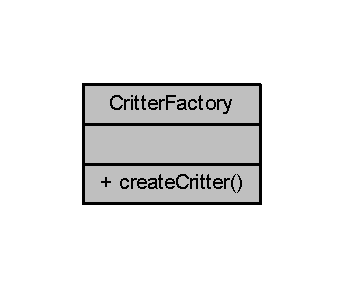
\includegraphics[width=165pt]{class_critter_factory__coll__graph}
\end{center}
\end{figure}
\subsection*{Static Public Member Functions}
\begin{DoxyCompactItemize}
\item 
static \hyperlink{class_critter}{Critter} $\ast$ \hyperlink{class_critter_factory_a3195f421d348fe4ee5c7e49e605745c1}{create\+Critter} (int id, \hyperlink{class_critter_acda8a5c3234b66101e0546d75d6f90f1}{Critter\+::\+Critter\+Type} type, \hyperlink{class_waypoint}{Waypoint} $\ast$starting\+\_\+waypoint)
\begin{DoxyCompactList}\small\item\em Factory method for \hyperlink{class_critter}{Critter} class. \end{DoxyCompactList}\end{DoxyCompactItemize}


\subsection{Detailed Description}
Creates objects derived from \hyperlink{class_critter}{Critter}. Utility class that creates instance of a \hyperlink{class_critter}{Critter} subclass from a family of derived \hyperlink{class_critter}{Critter} classes. 

\subsection{Member Function Documentation}
\hypertarget{class_critter_factory_a3195f421d348fe4ee5c7e49e605745c1}{\index{Critter\+Factory@{Critter\+Factory}!create\+Critter@{create\+Critter}}
\index{create\+Critter@{create\+Critter}!Critter\+Factory@{Critter\+Factory}}
\subsubsection[{create\+Critter}]{\setlength{\rightskip}{0pt plus 5cm}{\bf Critter} $\ast$ Critter\+Factory\+::create\+Critter (
\begin{DoxyParamCaption}
\item[{int}]{id, }
\item[{{\bf Critter\+::\+Critter\+Type}}]{type, }
\item[{{\bf Waypoint} $\ast$}]{starting\+\_\+waypoint}
\end{DoxyParamCaption}
)\hspace{0.3cm}{\ttfamily [static]}}}\label{class_critter_factory_a3195f421d348fe4ee5c7e49e605745c1}


Factory method for \hyperlink{class_critter}{Critter} class. 

\begin{DoxyReturn}{Returns}
\hyperlink{class_critter}{Critter} object (subclass of \hyperlink{class_critter}{Critter}).
\end{DoxyReturn}
The only method in \hyperlink{class_critter_factory}{Critter\+Factory}, \hyperlink{class_critter_factory_a3195f421d348fe4ee5c7e49e605745c1}{create\+Critter()} cranks out \hyperlink{class_critter}{Critter} objects based on the enum parameter. 

Here is the caller graph for this function\+:
\nopagebreak
\begin{figure}[H]
\begin{center}
\leavevmode
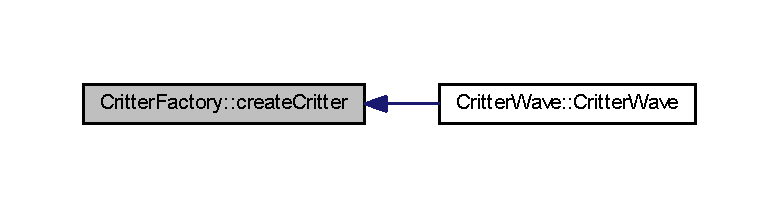
\includegraphics[width=350pt]{class_critter_factory_a3195f421d348fe4ee5c7e49e605745c1_icgraph}
\end{center}
\end{figure}




The documentation for this class was generated from the following files\+:\begin{DoxyCompactItemize}
\item 
jamms/\+Tower\+Defense/\+Tower\+Defense/include/game\+Objects/\hyperlink{_critter_factory_8h}{Critter\+Factory.\+h}\item 
jamms/\+Tower\+Defense/\+Tower\+Defense/src/game\+Objects/\hyperlink{_critter_factory_8cpp}{Critter\+Factory.\+cpp}\end{DoxyCompactItemize}

\hypertarget{class_critter_wave}{\section{Critter\+Wave Class Reference}
\label{class_critter_wave}\index{Critter\+Wave@{Critter\+Wave}}
}


Represents a wave of Critters. Class that has holds Critters in a map data structure, which represents a wave of Critters.  




{\ttfamily \#include $<$Critter\+Wave.\+h$>$}



Collaboration diagram for Critter\+Wave\+:\nopagebreak
\begin{figure}[H]
\begin{center}
\leavevmode
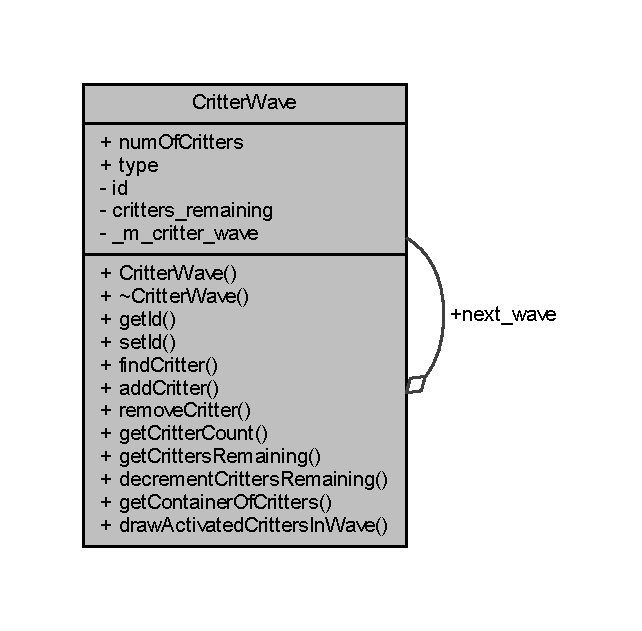
\includegraphics[width=308pt]{class_critter_wave__coll__graph}
\end{center}
\end{figure}
\subsection*{Classes}
\begin{DoxyCompactItemize}
\item 
struct \hyperlink{struct_critter_wave_1_1_critter_wave_deallocator}{Critter\+Wave\+Deallocator}
\begin{DoxyCompactList}\small\item\em Struct deallocating resources used in a \hyperlink{class_critter_wave}{Critter\+Wave} map. \end{DoxyCompactList}\end{DoxyCompactItemize}
\subsection*{Public Member Functions}
\begin{DoxyCompactItemize}
\item 
\hyperlink{class_critter_wave_a1364e3a7f9f4ab379847fe558b1fb233}{Critter\+Wave} (int \hyperlink{class_critter_wave_a6c8edb08492ed068c5e4c5323695c29d}{num\+Of\+Critters}, \hyperlink{class_critter_acda8a5c3234b66101e0546d75d6f90f1}{Critter\+::\+Critter\+Type} \hyperlink{class_critter_wave_aaf7c97d4f340ffa811ca452745ef6b24}{type}, \hyperlink{class_waypoint}{Waypoint} $\ast$starting\+\_\+waypoint)
\begin{DoxyCompactList}\small\item\em This constructor sets the type and number of critters for the wave. \end{DoxyCompactList}\item 
\hyperlink{class_critter_wave_a89e6acba97071ff44a9493315a8f073b}{$\sim$\+Critter\+Wave} ()
\begin{DoxyCompactList}\small\item\em This destructor iterates through the map, calling a deallocator which deletes Critter$\ast$ references in a wave. \end{DoxyCompactList}\item 
int \hyperlink{class_critter_wave_a127a4cc493bb6c6afcee3f394715b90d}{get\+Id} () const 
\item 
void \hyperlink{class_critter_wave_afcd7e16f4363b4be3be5649ef8325f55}{set\+Id} (int \hyperlink{class_critter_wave_aa476fc7af49dfb42fce07da5e726bbb2}{id})
\item 
\hyperlink{class_critter}{Critter} $\ast$ \hyperlink{class_critter_wave_a1244e59ebd702edd2530e6256779ace0}{find\+Critter} (int \hyperlink{class_critter_wave_aa476fc7af49dfb42fce07da5e726bbb2}{id}) const 
\begin{DoxyCompactList}\small\item\em Returns a reference to a \hyperlink{class_critter}{Critter} in the map. \end{DoxyCompactList}\item 
void \hyperlink{class_critter_wave_a3c6dcf79b57cb7e208471c5bc387f22d}{add\+Critter} (int \hyperlink{class_critter_wave_aa476fc7af49dfb42fce07da5e726bbb2}{id}, \hyperlink{class_critter}{Critter} $\ast$critter)
\begin{DoxyCompactList}\small\item\em Adding a \hyperlink{class_critter}{Critter} to the wave. \end{DoxyCompactList}\item 
void \hyperlink{class_critter_wave_aa7761b522b8774ef9b319861ae6ab844}{remove\+Critter} (int \hyperlink{class_critter_wave_aa476fc7af49dfb42fce07da5e726bbb2}{id})
\begin{DoxyCompactList}\small\item\em Remove a critter from the \hyperlink{class_critter_wave}{Critter\+Wave} map. \end{DoxyCompactList}\item 
int \hyperlink{class_critter_wave_a3c782475b9f1a73ddb658449592b8a33}{get\+Critter\+Count} () const 
\begin{DoxyCompactList}\small\item\em Returns how many critters are in a \hyperlink{class_critter_wave}{Critter\+Wave} map. \end{DoxyCompactList}\item 
int \hyperlink{class_critter_wave_af3879610de9f106cc80be0d7b4c1b1df}{get\+Critters\+Remaining} () const 
\item 
void \hyperlink{class_critter_wave_a14d2b9703371e82278c5fa3c4a2cbbd9}{decrement\+Critters\+Remaining} ()
\item 
std\+::map$<$ int, \hyperlink{class_critter}{Critter} $\ast$ $>$ \hyperlink{class_critter_wave_a00afecb75c04a7e0cd5073e20b11cce2}{get\+Container\+Of\+Critters} ()
\item 
void \hyperlink{class_critter_wave_a858c5934f74ac3148218e2f5a6a6e0b6}{draw\+Activated\+Critters\+In\+Wave} (sf\+::\+Render\+Window \&render\+\_\+window, float delta\+\_\+time)
\end{DoxyCompactItemize}
\subsection*{Public Attributes}
\begin{DoxyCompactItemize}
\item 
const int \hyperlink{class_critter_wave_a6c8edb08492ed068c5e4c5323695c29d}{num\+Of\+Critters}
\begin{DoxyCompactList}\small\item\em \hyperlink{class_map}{Map} representing a critter wave. \end{DoxyCompactList}\item 
\hyperlink{class_critter_acda8a5c3234b66101e0546d75d6f90f1}{Critter\+::\+Critter\+Type} \hyperlink{class_critter_wave_aaf7c97d4f340ffa811ca452745ef6b24}{type}
\begin{DoxyCompactList}\small\item\em Type of critter in a critter wave. \end{DoxyCompactList}\item 
\hyperlink{class_critter_wave}{Critter\+Wave} $\ast$ \hyperlink{class_critter_wave_a86ca5704a4a52a135fda195097dc4dd9}{next\+\_\+wave}
\begin{DoxyCompactList}\small\item\em Pointer to the next \hyperlink{class_critter_wave}{Critter\+Wave}. \end{DoxyCompactList}\end{DoxyCompactItemize}
\subsection*{Private Attributes}
\begin{DoxyCompactItemize}
\item 
int \hyperlink{class_critter_wave_aa476fc7af49dfb42fce07da5e726bbb2}{id}
\item 
int \hyperlink{class_critter_wave_a6fea77f30895b8ac455dd25a4287abd6}{critters\+\_\+remaining}
\item 
std\+::map$<$ int, \hyperlink{class_critter}{Critter} $\ast$ $>$ \hyperlink{class_critter_wave_a82475869f718062181e545afb8277217}{\+\_\+m\+\_\+critter\+\_\+wave}
\begin{DoxyCompactList}\small\item\em \hyperlink{class_map}{Map} representing a critter wave. \end{DoxyCompactList}\end{DoxyCompactItemize}
\subsection*{Friends}
\begin{DoxyCompactItemize}
\item 
std\+::ostream \& \hyperlink{class_critter_wave_a06016c30b019307c3fd6e11c447ffbe0}{operator$<$$<$} (std\+::ostream \&output, const \hyperlink{class_critter_wave}{Critter\+Wave} \&critter\+\_\+wave)
\begin{DoxyCompactList}\small\item\em Overloaded cout operator to print out Critter\+Waves. \end{DoxyCompactList}\end{DoxyCompactItemize}


\subsection{Detailed Description}
Represents a wave of Critters. Class that has holds Critters in a map data structure, which represents a wave of Critters. 

\subsection{Constructor \& Destructor Documentation}
\hypertarget{class_critter_wave_a1364e3a7f9f4ab379847fe558b1fb233}{\index{Critter\+Wave@{Critter\+Wave}!Critter\+Wave@{Critter\+Wave}}
\index{Critter\+Wave@{Critter\+Wave}!Critter\+Wave@{Critter\+Wave}}
\subsubsection[{Critter\+Wave}]{\setlength{\rightskip}{0pt plus 5cm}Critter\+Wave\+::\+Critter\+Wave (
\begin{DoxyParamCaption}
\item[{int}]{num\+Of\+Critters, }
\item[{{\bf Critter\+::\+Critter\+Type}}]{type, }
\item[{{\bf Waypoint} $\ast$}]{starting\+\_\+waypoint}
\end{DoxyParamCaption}
)}}\label{class_critter_wave_a1364e3a7f9f4ab379847fe558b1fb233}


This constructor sets the type and number of critters for the wave. 



Here is the call graph for this function\+:\nopagebreak
\begin{figure}[H]
\begin{center}
\leavevmode
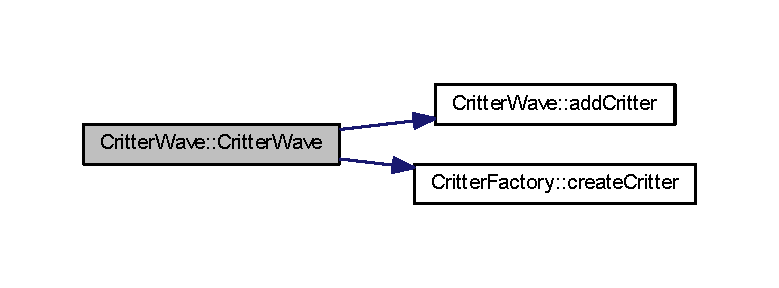
\includegraphics[width=350pt]{class_critter_wave_a1364e3a7f9f4ab379847fe558b1fb233_cgraph}
\end{center}
\end{figure}


\hypertarget{class_critter_wave_a89e6acba97071ff44a9493315a8f073b}{\index{Critter\+Wave@{Critter\+Wave}!````~Critter\+Wave@{$\sim$\+Critter\+Wave}}
\index{````~Critter\+Wave@{$\sim$\+Critter\+Wave}!Critter\+Wave@{Critter\+Wave}}
\subsubsection[{$\sim$\+Critter\+Wave}]{\setlength{\rightskip}{0pt plus 5cm}Critter\+Wave\+::$\sim$\+Critter\+Wave (
\begin{DoxyParamCaption}
{}
\end{DoxyParamCaption}
)}}\label{class_critter_wave_a89e6acba97071ff44a9493315a8f073b}


This destructor iterates through the map, calling a deallocator which deletes Critter$\ast$ references in a wave. 



\subsection{Member Function Documentation}
\hypertarget{class_critter_wave_a3c6dcf79b57cb7e208471c5bc387f22d}{\index{Critter\+Wave@{Critter\+Wave}!add\+Critter@{add\+Critter}}
\index{add\+Critter@{add\+Critter}!Critter\+Wave@{Critter\+Wave}}
\subsubsection[{add\+Critter}]{\setlength{\rightskip}{0pt plus 5cm}void Critter\+Wave\+::add\+Critter (
\begin{DoxyParamCaption}
\item[{int}]{id, }
\item[{{\bf Critter} $\ast$}]{critter}
\end{DoxyParamCaption}
)}}\label{class_critter_wave_a3c6dcf79b57cb7e208471c5bc387f22d}


Adding a \hyperlink{class_critter}{Critter} to the wave. 



Here is the caller graph for this function\+:\nopagebreak
\begin{figure}[H]
\begin{center}
\leavevmode
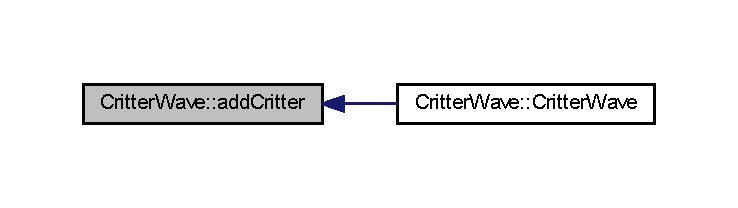
\includegraphics[width=350pt]{class_critter_wave_a3c6dcf79b57cb7e208471c5bc387f22d_icgraph}
\end{center}
\end{figure}


\hypertarget{class_critter_wave_a14d2b9703371e82278c5fa3c4a2cbbd9}{\index{Critter\+Wave@{Critter\+Wave}!decrement\+Critters\+Remaining@{decrement\+Critters\+Remaining}}
\index{decrement\+Critters\+Remaining@{decrement\+Critters\+Remaining}!Critter\+Wave@{Critter\+Wave}}
\subsubsection[{decrement\+Critters\+Remaining}]{\setlength{\rightskip}{0pt plus 5cm}void Critter\+Wave\+::decrement\+Critters\+Remaining (
\begin{DoxyParamCaption}
{}
\end{DoxyParamCaption}
)}}\label{class_critter_wave_a14d2b9703371e82278c5fa3c4a2cbbd9}


Here is the caller graph for this function\+:
\nopagebreak
\begin{figure}[H]
\begin{center}
\leavevmode
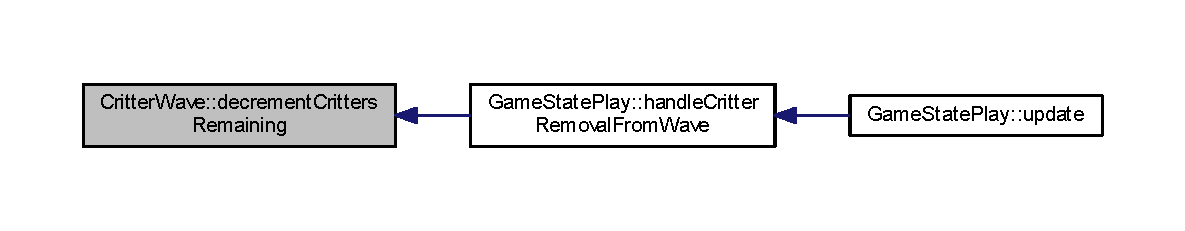
\includegraphics[width=350pt]{class_critter_wave_a14d2b9703371e82278c5fa3c4a2cbbd9_icgraph}
\end{center}
\end{figure}


\hypertarget{class_critter_wave_a858c5934f74ac3148218e2f5a6a6e0b6}{\index{Critter\+Wave@{Critter\+Wave}!draw\+Activated\+Critters\+In\+Wave@{draw\+Activated\+Critters\+In\+Wave}}
\index{draw\+Activated\+Critters\+In\+Wave@{draw\+Activated\+Critters\+In\+Wave}!Critter\+Wave@{Critter\+Wave}}
\subsubsection[{draw\+Activated\+Critters\+In\+Wave}]{\setlength{\rightskip}{0pt plus 5cm}void Critter\+Wave\+::draw\+Activated\+Critters\+In\+Wave (
\begin{DoxyParamCaption}
\item[{sf\+::\+Render\+Window \&}]{render\+\_\+window, }
\item[{float}]{delta\+\_\+time}
\end{DoxyParamCaption}
)}}\label{class_critter_wave_a858c5934f74ac3148218e2f5a6a6e0b6}


Here is the caller graph for this function\+:\nopagebreak
\begin{figure}[H]
\begin{center}
\leavevmode
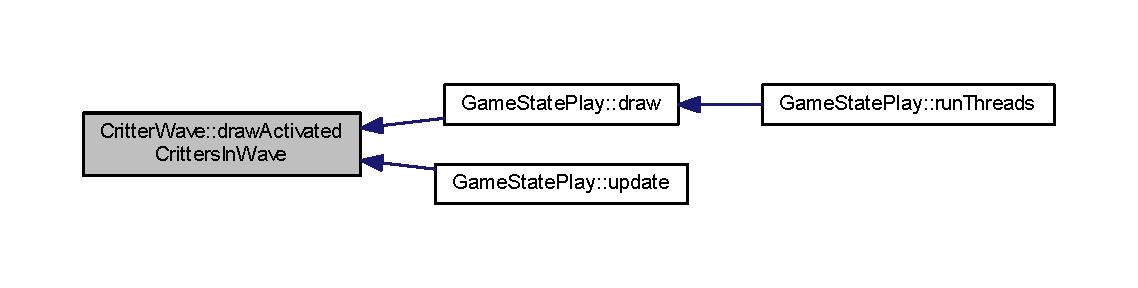
\includegraphics[width=350pt]{class_critter_wave_a858c5934f74ac3148218e2f5a6a6e0b6_icgraph}
\end{center}
\end{figure}


\hypertarget{class_critter_wave_a1244e59ebd702edd2530e6256779ace0}{\index{Critter\+Wave@{Critter\+Wave}!find\+Critter@{find\+Critter}}
\index{find\+Critter@{find\+Critter}!Critter\+Wave@{Critter\+Wave}}
\subsubsection[{find\+Critter}]{\setlength{\rightskip}{0pt plus 5cm}{\bf Critter} $\ast$ Critter\+Wave\+::find\+Critter (
\begin{DoxyParamCaption}
\item[{int}]{id}
\end{DoxyParamCaption}
) const}}\label{class_critter_wave_a1244e59ebd702edd2530e6256779ace0}


Returns a reference to a \hyperlink{class_critter}{Critter} in the map. 


\begin{DoxyParams}{Parameters}
{\em critter\+\_\+id} & Id of the \hyperlink{class_critter}{Critter} to be found \\
\hline
\end{DoxyParams}
\begin{DoxyReturn}{Returns}
Pointer to a \hyperlink{class_critter}{Critter} in the map.
\end{DoxyReturn}
Iterate through the map, looking for the given \hyperlink{class_critter}{Critter} id. If end of map is reached, return null, else return the Critter$\ast$. 

Here is the caller graph for this function\+:\nopagebreak
\begin{figure}[H]
\begin{center}
\leavevmode
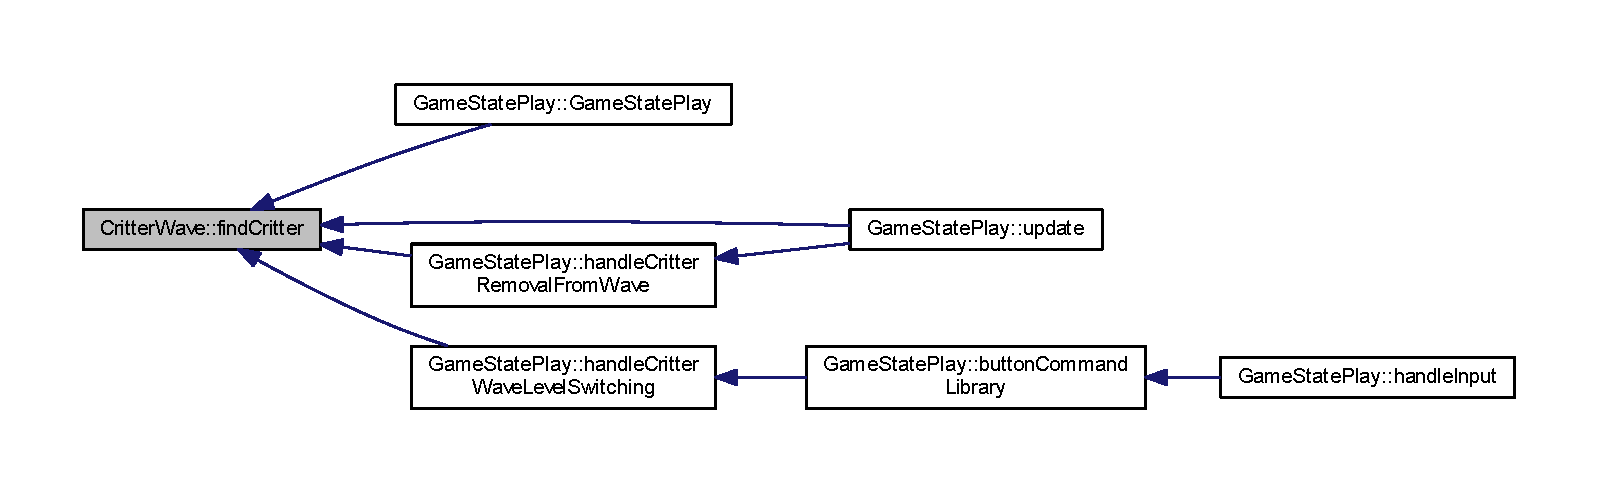
\includegraphics[width=350pt]{class_critter_wave_a1244e59ebd702edd2530e6256779ace0_icgraph}
\end{center}
\end{figure}


\hypertarget{class_critter_wave_a00afecb75c04a7e0cd5073e20b11cce2}{\index{Critter\+Wave@{Critter\+Wave}!get\+Container\+Of\+Critters@{get\+Container\+Of\+Critters}}
\index{get\+Container\+Of\+Critters@{get\+Container\+Of\+Critters}!Critter\+Wave@{Critter\+Wave}}
\subsubsection[{get\+Container\+Of\+Critters}]{\setlength{\rightskip}{0pt plus 5cm}std\+::map$<$ int, {\bf Critter} $\ast$ $>$ Critter\+Wave\+::get\+Container\+Of\+Critters (
\begin{DoxyParamCaption}
{}
\end{DoxyParamCaption}
)}}\label{class_critter_wave_a00afecb75c04a7e0cd5073e20b11cce2}


Here is the caller graph for this function\+:
\nopagebreak
\begin{figure}[H]
\begin{center}
\leavevmode
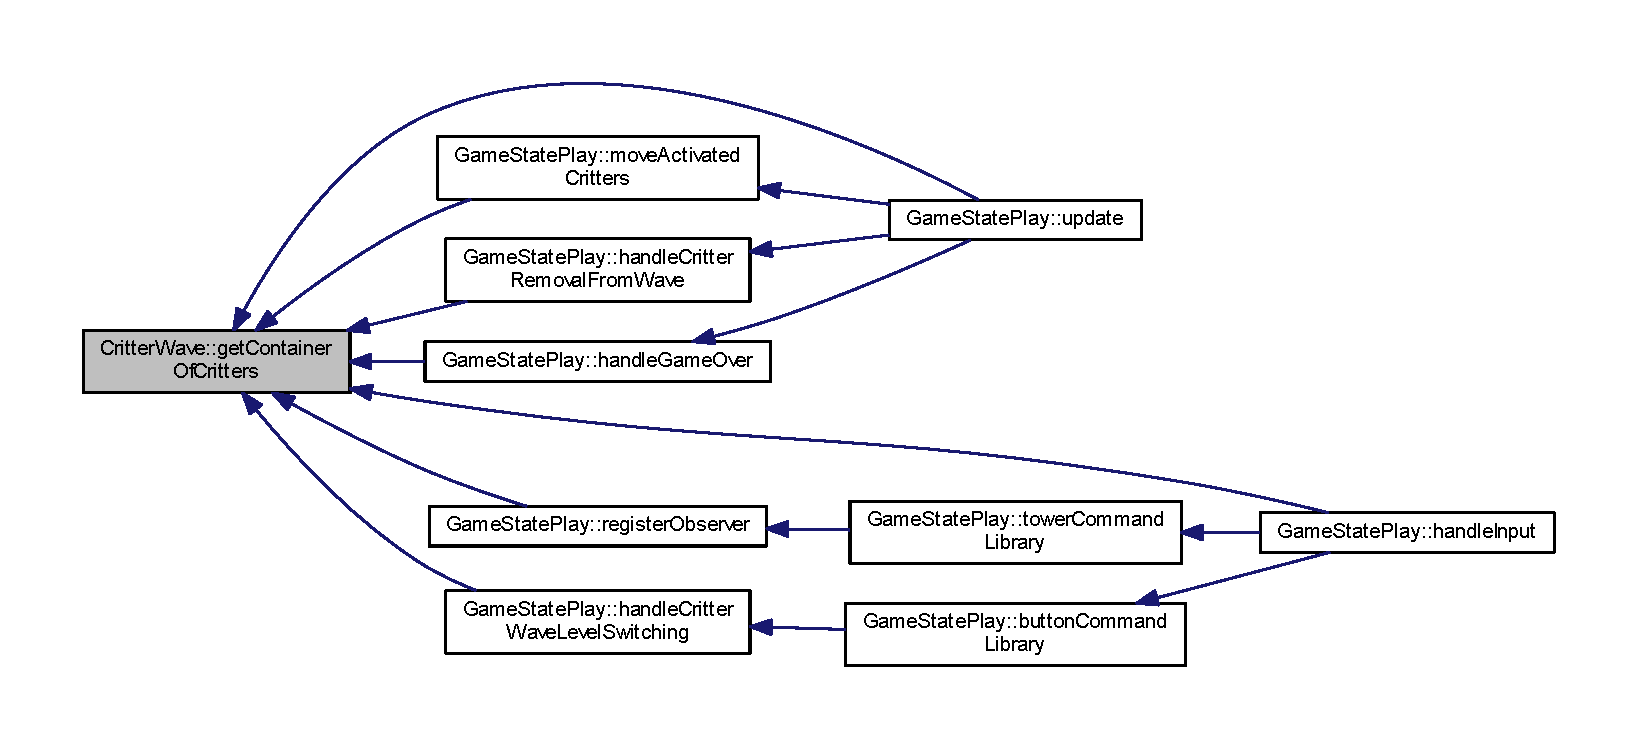
\includegraphics[width=350pt]{class_critter_wave_a00afecb75c04a7e0cd5073e20b11cce2_icgraph}
\end{center}
\end{figure}


\hypertarget{class_critter_wave_a3c782475b9f1a73ddb658449592b8a33}{\index{Critter\+Wave@{Critter\+Wave}!get\+Critter\+Count@{get\+Critter\+Count}}
\index{get\+Critter\+Count@{get\+Critter\+Count}!Critter\+Wave@{Critter\+Wave}}
\subsubsection[{get\+Critter\+Count}]{\setlength{\rightskip}{0pt plus 5cm}int Critter\+Wave\+::get\+Critter\+Count (
\begin{DoxyParamCaption}
{}
\end{DoxyParamCaption}
) const}}\label{class_critter_wave_a3c782475b9f1a73ddb658449592b8a33}


Returns how many critters are in a \hyperlink{class_critter_wave}{Critter\+Wave} map. 

\begin{DoxyReturn}{Returns}
Count of number of Critters in a wave. 
\end{DoxyReturn}
\hypertarget{class_critter_wave_af3879610de9f106cc80be0d7b4c1b1df}{\index{Critter\+Wave@{Critter\+Wave}!get\+Critters\+Remaining@{get\+Critters\+Remaining}}
\index{get\+Critters\+Remaining@{get\+Critters\+Remaining}!Critter\+Wave@{Critter\+Wave}}
\subsubsection[{get\+Critters\+Remaining}]{\setlength{\rightskip}{0pt plus 5cm}int Critter\+Wave\+::get\+Critters\+Remaining (
\begin{DoxyParamCaption}
{}
\end{DoxyParamCaption}
) const}}\label{class_critter_wave_af3879610de9f106cc80be0d7b4c1b1df}


Here is the caller graph for this function\+:\nopagebreak
\begin{figure}[H]
\begin{center}
\leavevmode
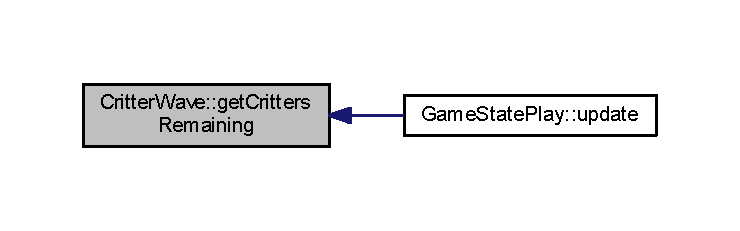
\includegraphics[width=350pt]{class_critter_wave_af3879610de9f106cc80be0d7b4c1b1df_icgraph}
\end{center}
\end{figure}


\hypertarget{class_critter_wave_a127a4cc493bb6c6afcee3f394715b90d}{\index{Critter\+Wave@{Critter\+Wave}!get\+Id@{get\+Id}}
\index{get\+Id@{get\+Id}!Critter\+Wave@{Critter\+Wave}}
\subsubsection[{get\+Id}]{\setlength{\rightskip}{0pt plus 5cm}int Critter\+Wave\+::get\+Id (
\begin{DoxyParamCaption}
{}
\end{DoxyParamCaption}
) const}}\label{class_critter_wave_a127a4cc493bb6c6afcee3f394715b90d}


Here is the caller graph for this function\+:\nopagebreak
\begin{figure}[H]
\begin{center}
\leavevmode
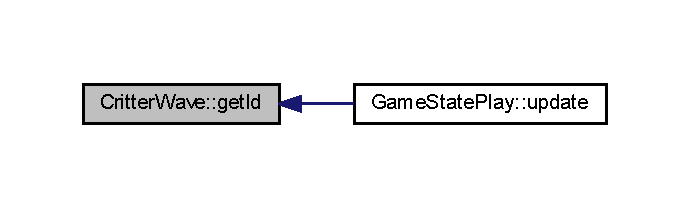
\includegraphics[width=331pt]{class_critter_wave_a127a4cc493bb6c6afcee3f394715b90d_icgraph}
\end{center}
\end{figure}


\hypertarget{class_critter_wave_aa7761b522b8774ef9b319861ae6ab844}{\index{Critter\+Wave@{Critter\+Wave}!remove\+Critter@{remove\+Critter}}
\index{remove\+Critter@{remove\+Critter}!Critter\+Wave@{Critter\+Wave}}
\subsubsection[{remove\+Critter}]{\setlength{\rightskip}{0pt plus 5cm}void Critter\+Wave\+::remove\+Critter (
\begin{DoxyParamCaption}
\item[{int}]{id}
\end{DoxyParamCaption}
)}}\label{class_critter_wave_aa7761b522b8774ef9b319861ae6ab844}


Remove a critter from the \hyperlink{class_critter_wave}{Critter\+Wave} map. 


\begin{DoxyParams}{Parameters}
{\em critter\+\_\+id} & Id of the \hyperlink{class_critter}{Critter} to be removed\\
\hline
\end{DoxyParams}
Iterate through the map, looking for the given \hyperlink{class_critter}{Critter} id, if found, delete the pointer and remove the Critter$\ast$ from the map. \hypertarget{class_critter_wave_afcd7e16f4363b4be3be5649ef8325f55}{\index{Critter\+Wave@{Critter\+Wave}!set\+Id@{set\+Id}}
\index{set\+Id@{set\+Id}!Critter\+Wave@{Critter\+Wave}}
\subsubsection[{set\+Id}]{\setlength{\rightskip}{0pt plus 5cm}void Critter\+Wave\+::set\+Id (
\begin{DoxyParamCaption}
\item[{int}]{id}
\end{DoxyParamCaption}
)}}\label{class_critter_wave_afcd7e16f4363b4be3be5649ef8325f55}


\subsection{Friends And Related Function Documentation}
\hypertarget{class_critter_wave_a06016c30b019307c3fd6e11c447ffbe0}{\index{Critter\+Wave@{Critter\+Wave}!operator$<$$<$@{operator$<$$<$}}
\index{operator$<$$<$@{operator$<$$<$}!Critter\+Wave@{Critter\+Wave}}
\subsubsection[{operator$<$$<$}]{\setlength{\rightskip}{0pt plus 5cm}std\+::ostream\& operator$<$$<$ (
\begin{DoxyParamCaption}
\item[{std\+::ostream \&}]{output, }
\item[{const {\bf Critter\+Wave} \&}]{critter\+\_\+wave}
\end{DoxyParamCaption}
)\hspace{0.3cm}{\ttfamily [friend]}}}\label{class_critter_wave_a06016c30b019307c3fd6e11c447ffbe0}


Overloaded cout operator to print out Critter\+Waves. 


\begin{DoxyParams}{Parameters}
{\em output} & Output stream address \\
\hline
{\em critter} & Const address to \hyperlink{class_critter_wave}{Critter\+Wave} \\
\hline
\end{DoxyParams}
\begin{DoxyReturn}{Returns}
Address to output stream 
\end{DoxyReturn}


\subsection{Member Data Documentation}
\hypertarget{class_critter_wave_a82475869f718062181e545afb8277217}{\index{Critter\+Wave@{Critter\+Wave}!\+\_\+m\+\_\+critter\+\_\+wave@{\+\_\+m\+\_\+critter\+\_\+wave}}
\index{\+\_\+m\+\_\+critter\+\_\+wave@{\+\_\+m\+\_\+critter\+\_\+wave}!Critter\+Wave@{Critter\+Wave}}
\subsubsection[{\+\_\+m\+\_\+critter\+\_\+wave}]{\setlength{\rightskip}{0pt plus 5cm}std\+::map$<$int, {\bf Critter}$\ast$$>$ Critter\+Wave\+::\+\_\+m\+\_\+critter\+\_\+wave\hspace{0.3cm}{\ttfamily [private]}}}\label{class_critter_wave_a82475869f718062181e545afb8277217}


\hyperlink{class_map}{Map} representing a critter wave. 

\hypertarget{class_critter_wave_a6fea77f30895b8ac455dd25a4287abd6}{\index{Critter\+Wave@{Critter\+Wave}!critters\+\_\+remaining@{critters\+\_\+remaining}}
\index{critters\+\_\+remaining@{critters\+\_\+remaining}!Critter\+Wave@{Critter\+Wave}}
\subsubsection[{critters\+\_\+remaining}]{\setlength{\rightskip}{0pt plus 5cm}int Critter\+Wave\+::critters\+\_\+remaining\hspace{0.3cm}{\ttfamily [private]}}}\label{class_critter_wave_a6fea77f30895b8ac455dd25a4287abd6}
\hypertarget{class_critter_wave_aa476fc7af49dfb42fce07da5e726bbb2}{\index{Critter\+Wave@{Critter\+Wave}!id@{id}}
\index{id@{id}!Critter\+Wave@{Critter\+Wave}}
\subsubsection[{id}]{\setlength{\rightskip}{0pt plus 5cm}int Critter\+Wave\+::id\hspace{0.3cm}{\ttfamily [private]}}}\label{class_critter_wave_aa476fc7af49dfb42fce07da5e726bbb2}
\hypertarget{class_critter_wave_a86ca5704a4a52a135fda195097dc4dd9}{\index{Critter\+Wave@{Critter\+Wave}!next\+\_\+wave@{next\+\_\+wave}}
\index{next\+\_\+wave@{next\+\_\+wave}!Critter\+Wave@{Critter\+Wave}}
\subsubsection[{next\+\_\+wave}]{\setlength{\rightskip}{0pt plus 5cm}{\bf Critter\+Wave}$\ast$ Critter\+Wave\+::next\+\_\+wave}}\label{class_critter_wave_a86ca5704a4a52a135fda195097dc4dd9}


Pointer to the next \hyperlink{class_critter_wave}{Critter\+Wave}. 

\hypertarget{class_critter_wave_a6c8edb08492ed068c5e4c5323695c29d}{\index{Critter\+Wave@{Critter\+Wave}!num\+Of\+Critters@{num\+Of\+Critters}}
\index{num\+Of\+Critters@{num\+Of\+Critters}!Critter\+Wave@{Critter\+Wave}}
\subsubsection[{num\+Of\+Critters}]{\setlength{\rightskip}{0pt plus 5cm}const int Critter\+Wave\+::num\+Of\+Critters}}\label{class_critter_wave_a6c8edb08492ed068c5e4c5323695c29d}


\hyperlink{class_map}{Map} representing a critter wave. 

\hypertarget{class_critter_wave_aaf7c97d4f340ffa811ca452745ef6b24}{\index{Critter\+Wave@{Critter\+Wave}!type@{type}}
\index{type@{type}!Critter\+Wave@{Critter\+Wave}}
\subsubsection[{type}]{\setlength{\rightskip}{0pt plus 5cm}{\bf Critter\+::\+Critter\+Type} Critter\+Wave\+::type}}\label{class_critter_wave_aaf7c97d4f340ffa811ca452745ef6b24}


Type of critter in a critter wave. 



The documentation for this class was generated from the following files\+:\begin{DoxyCompactItemize}
\item 
jamms/\+Tower\+Defense/\+Tower\+Defense/include/managers/\hyperlink{_critter_wave_8h}{Critter\+Wave.\+h}\item 
jamms/\+Tower\+Defense/\+Tower\+Defense/src/managers/\hyperlink{_critter_wave_8cpp}{Critter\+Wave.\+cpp}\end{DoxyCompactItemize}

\hypertarget{struct_critter_wave_1_1_critter_wave_deallocator}{\section{Critter\+Wave\+:\+:Critter\+Wave\+Deallocator Struct Reference}
\label{struct_critter_wave_1_1_critter_wave_deallocator}\index{Critter\+Wave\+::\+Critter\+Wave\+Deallocator@{Critter\+Wave\+::\+Critter\+Wave\+Deallocator}}
}


Struct deallocating resources used in a \hyperlink{class_critter_wave}{Critter\+Wave} map.  




Collaboration diagram for Critter\+Wave\+:\+:Critter\+Wave\+Deallocator\+:
\nopagebreak
\begin{figure}[H]
\begin{center}
\leavevmode
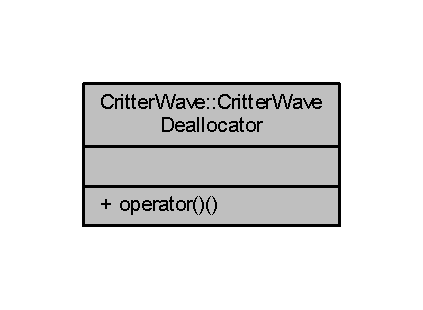
\includegraphics[width=203pt]{struct_critter_wave_1_1_critter_wave_deallocator__coll__graph}
\end{center}
\end{figure}
\subsection*{Public Member Functions}
\begin{DoxyCompactItemize}
\item 
void \hyperlink{struct_critter_wave_1_1_critter_wave_deallocator_a3b5befe161e66cd3d7cf9d72b948cd6a}{operator()} (const std\+::pair$<$ int, \hyperlink{class_critter}{Critter} $\ast$ $>$ \&item)
\begin{DoxyCompactList}\small\item\em Overloading of the function operator () \end{DoxyCompactList}\end{DoxyCompactItemize}


\subsection{Detailed Description}
Struct deallocating resources used in a \hyperlink{class_critter_wave}{Critter\+Wave} map. 

\subsection{Member Function Documentation}
\hypertarget{struct_critter_wave_1_1_critter_wave_deallocator_a3b5befe161e66cd3d7cf9d72b948cd6a}{\index{Critter\+Wave\+::\+Critter\+Wave\+Deallocator@{Critter\+Wave\+::\+Critter\+Wave\+Deallocator}!operator()@{operator()}}
\index{operator()@{operator()}!Critter\+Wave\+::\+Critter\+Wave\+Deallocator@{Critter\+Wave\+::\+Critter\+Wave\+Deallocator}}
\subsubsection[{operator()}]{\setlength{\rightskip}{0pt plus 5cm}void Critter\+Wave\+::\+Critter\+Wave\+Deallocator\+::operator() (
\begin{DoxyParamCaption}
\item[{const std\+::pair$<$ int, {\bf Critter} $\ast$ $>$ \&}]{item}
\end{DoxyParamCaption}
)\hspace{0.3cm}{\ttfamily [inline]}}}\label{struct_critter_wave_1_1_critter_wave_deallocator_a3b5befe161e66cd3d7cf9d72b948cd6a}


Overloading of the function operator () 


\begin{DoxyParams}{Parameters}
{\em item} & Coupled values that represents an item in the map \\
\hline
\end{DoxyParams}
\begin{DoxyReturn}{Returns}
Void. 
\end{DoxyReturn}


The documentation for this struct was generated from the following file\+:\begin{DoxyCompactItemize}
\item 
jamms/\+Tower\+Defense/\+Tower\+Defense/include/managers/\hyperlink{_critter_wave_8h}{Critter\+Wave.\+h}\end{DoxyCompactItemize}

\hypertarget{class_dalmatian}{\section{Dalmatian Class Reference}
\label{class_dalmatian}\index{Dalmatian@{Dalmatian}}
}


{\ttfamily \#include $<$Dalmatian.\+h$>$}



Inheritance diagram for Dalmatian\+:
\nopagebreak
\begin{figure}[H]
\begin{center}
\leavevmode
\includegraphics[height=550pt]{class_dalmatian__inherit__graph}
\end{center}
\end{figure}


Collaboration diagram for Dalmatian\+:
\nopagebreak
\begin{figure}[H]
\begin{center}
\leavevmode
\includegraphics[height=550pt]{class_dalmatian__coll__graph}
\end{center}
\end{figure}
\subsection*{Public Member Functions}
\begin{DoxyCompactItemize}
\item 
\hyperlink{class_dalmatian_ab4ce8123d58ef775d1bc80b72485a77d}{Dalmatian} (int tile\+X, int tile\+Y)
\item 
void \hyperlink{class_dalmatian_aa87cd8b4c763d84d24964024bde2fc9b}{upgrade\+Tower} ()
\end{DoxyCompactItemize}
\subsection*{Additional Inherited Members}


\subsection{Constructor \& Destructor Documentation}
\hypertarget{class_dalmatian_ab4ce8123d58ef775d1bc80b72485a77d}{\index{Dalmatian@{Dalmatian}!Dalmatian@{Dalmatian}}
\index{Dalmatian@{Dalmatian}!Dalmatian@{Dalmatian}}
\subsubsection[{Dalmatian}]{\setlength{\rightskip}{0pt plus 5cm}Dalmatian\+::\+Dalmatian (
\begin{DoxyParamCaption}
\item[{int}]{tile\+X, }
\item[{int}]{tile\+Y}
\end{DoxyParamCaption}
)}}\label{class_dalmatian_ab4ce8123d58ef775d1bc80b72485a77d}


Here is the call graph for this function\+:
\nopagebreak
\begin{figure}[H]
\begin{center}
\leavevmode
\includegraphics[width=350pt]{class_dalmatian_ab4ce8123d58ef775d1bc80b72485a77d_cgraph}
\end{center}
\end{figure}




\subsection{Member Function Documentation}
\hypertarget{class_dalmatian_aa87cd8b4c763d84d24964024bde2fc9b}{\index{Dalmatian@{Dalmatian}!upgrade\+Tower@{upgrade\+Tower}}
\index{upgrade\+Tower@{upgrade\+Tower}!Dalmatian@{Dalmatian}}
\subsubsection[{upgrade\+Tower}]{\setlength{\rightskip}{0pt plus 5cm}void Dalmatian\+::upgrade\+Tower (
\begin{DoxyParamCaption}
{}
\end{DoxyParamCaption}
)\hspace{0.3cm}{\ttfamily [virtual]}}}\label{class_dalmatian_aa87cd8b4c763d84d24964024bde2fc9b}


Implements \hyperlink{class_tower_a06801dd47796aaa9942fb3d890d2196a}{Tower}.



Here is the call graph for this function\+:
\nopagebreak
\begin{figure}[H]
\begin{center}
\leavevmode
\includegraphics[width=350pt]{class_dalmatian_aa87cd8b4c763d84d24964024bde2fc9b_cgraph}
\end{center}
\end{figure}




The documentation for this class was generated from the following files\+:\begin{DoxyCompactItemize}
\item 
jamms/\+Tower\+Defense/\+Tower\+Defense/include/game\+Objects/\hyperlink{_dalmatian_8h}{Dalmatian.\+h}\item 
jamms/\+Tower\+Defense/\+Tower\+Defense/src/game\+Objects/\hyperlink{_dalmatian_8cpp}{Dalmatian.\+cpp}\end{DoxyCompactItemize}

\hypertarget{class_dead_tile}{\section{Dead\+Tile Class Reference}
\label{class_dead_tile}\index{Dead\+Tile@{Dead\+Tile}}
}


{\ttfamily \#include $<$Tile.\+h$>$}



Inheritance diagram for Dead\+Tile\+:
\nopagebreak
\begin{figure}[H]
\begin{center}
\leavevmode
\includegraphics[height=550pt]{class_dead_tile__inherit__graph}
\end{center}
\end{figure}


Collaboration diagram for Dead\+Tile\+:
\nopagebreak
\begin{figure}[H]
\begin{center}
\leavevmode
\includegraphics[height=550pt]{class_dead_tile__coll__graph}
\end{center}
\end{figure}
\subsection*{Public Member Functions}
\begin{DoxyCompactItemize}
\item 
\hyperlink{class_dead_tile_a02f167ebcda600d8a05ce2c643b30739}{Dead\+Tile} (const string texture\+I\+D, int \hyperlink{class_tile_ac3f88f7a9c6ec1d0c9640ebb9a6ae73a}{tile\+X}, int \hyperlink{class_tile_a3fbe8c6bce65bc408ae0d028e43f4672}{tile\+Y})
\item 
virtual \hyperlink{class_dead_tile_a8950ac37c340504c5e3a43d8f6c412e0}{$\sim$\+Dead\+Tile} ()
\end{DoxyCompactItemize}
\subsection*{Additional Inherited Members}


\subsection{Constructor \& Destructor Documentation}
\hypertarget{class_dead_tile_a02f167ebcda600d8a05ce2c643b30739}{\index{Dead\+Tile@{Dead\+Tile}!Dead\+Tile@{Dead\+Tile}}
\index{Dead\+Tile@{Dead\+Tile}!Dead\+Tile@{Dead\+Tile}}
\subsubsection[{Dead\+Tile}]{\setlength{\rightskip}{0pt plus 5cm}Dead\+Tile\+::\+Dead\+Tile (
\begin{DoxyParamCaption}
\item[{const string}]{texture\+I\+D, }
\item[{int}]{tile\+X, }
\item[{int}]{tile\+Y}
\end{DoxyParamCaption}
)}}\label{class_dead_tile_a02f167ebcda600d8a05ce2c643b30739}


Here is the call graph for this function\+:\nopagebreak
\begin{figure}[H]
\begin{center}
\leavevmode
\includegraphics[width=286pt]{class_dead_tile_a02f167ebcda600d8a05ce2c643b30739_cgraph}
\end{center}
\end{figure}


\hypertarget{class_dead_tile_a8950ac37c340504c5e3a43d8f6c412e0}{\index{Dead\+Tile@{Dead\+Tile}!````~Dead\+Tile@{$\sim$\+Dead\+Tile}}
\index{````~Dead\+Tile@{$\sim$\+Dead\+Tile}!Dead\+Tile@{Dead\+Tile}}
\subsubsection[{$\sim$\+Dead\+Tile}]{\setlength{\rightskip}{0pt plus 5cm}Dead\+Tile\+::$\sim$\+Dead\+Tile (
\begin{DoxyParamCaption}
{}
\end{DoxyParamCaption}
)\hspace{0.3cm}{\ttfamily [virtual]}}}\label{class_dead_tile_a8950ac37c340504c5e3a43d8f6c412e0}


The documentation for this class was generated from the following files\+:\begin{DoxyCompactItemize}
\item 
jamms/\+Tower\+Defense/\+Tower\+Defense/include/game\+Objects/\hyperlink{_tile_8h}{Tile.\+h}\item 
jamms/\+Tower\+Defense/\+Tower\+Defense/src/game\+Objects/\hyperlink{_tile_8cpp}{Tile.\+cpp}\end{DoxyCompactItemize}

\hypertarget{struct_d_i_r}{\section{D\+I\+R Struct Reference}
\label{struct_d_i_r}\index{D\+I\+R@{D\+I\+R}}
}


{\ttfamily \#include $<$dirent.\+h$>$}



Collaboration diagram for D\+I\+R\+:
\nopagebreak
\begin{figure}[H]
\begin{center}
\leavevmode
\includegraphics[width=229pt]{struct_d_i_r__coll__graph}
\end{center}
\end{figure}
\subsection*{Public Attributes}
\begin{DoxyCompactItemize}
\item 
struct \hyperlink{structdirent}{dirent} \hyperlink{struct_d_i_r_a59e9f5211cbb2f8e5b2807ccfdd2a7fc}{ent}
\item 
struct \hyperlink{struct___w_d_i_r}{\+\_\+\+W\+D\+I\+R} $\ast$ \hyperlink{struct_d_i_r_a29362d4a3d7f809d0f5418b26cac5d41}{wdirp}
\end{DoxyCompactItemize}


\subsection{Member Data Documentation}
\hypertarget{struct_d_i_r_a59e9f5211cbb2f8e5b2807ccfdd2a7fc}{\index{D\+I\+R@{D\+I\+R}!ent@{ent}}
\index{ent@{ent}!D\+I\+R@{D\+I\+R}}
\subsubsection[{ent}]{\setlength{\rightskip}{0pt plus 5cm}struct {\bf dirent} D\+I\+R\+::ent}}\label{struct_d_i_r_a59e9f5211cbb2f8e5b2807ccfdd2a7fc}
\hypertarget{struct_d_i_r_a29362d4a3d7f809d0f5418b26cac5d41}{\index{D\+I\+R@{D\+I\+R}!wdirp@{wdirp}}
\index{wdirp@{wdirp}!D\+I\+R@{D\+I\+R}}
\subsubsection[{wdirp}]{\setlength{\rightskip}{0pt plus 5cm}struct {\bf \+\_\+\+W\+D\+I\+R}$\ast$ D\+I\+R\+::wdirp}}\label{struct_d_i_r_a29362d4a3d7f809d0f5418b26cac5d41}


The documentation for this struct was generated from the following file\+:\begin{DoxyCompactItemize}
\item 
jamms/\+Tower\+Defense/\+Tower\+Defense/include/\hyperlink{dirent_8h}{dirent.\+h}\end{DoxyCompactItemize}

\hypertarget{structdirent}{\section{dirent Struct Reference}
\label{structdirent}\index{dirent@{dirent}}
}


{\ttfamily \#include $<$dirent.\+h$>$}



Collaboration diagram for dirent\+:
\nopagebreak
\begin{figure}[H]
\begin{center}
\leavevmode
\includegraphics[width=148pt]{structdirent__coll__graph}
\end{center}
\end{figure}
\subsection*{Public Attributes}
\begin{DoxyCompactItemize}
\item 
long \hyperlink{structdirent_acb6fecfb0e0f6fdc226dff8d56c3da4a}{d\+\_\+ino}
\item 
unsigned short \hyperlink{structdirent_a90dc47836e8ef510437317876368859e}{d\+\_\+reclen}
\item 
size\+\_\+t \hyperlink{structdirent_a09ced068b03cdb339e34840c8b709621}{d\+\_\+namlen}
\item 
int \hyperlink{structdirent_ad6a736cb04c7295e8f97f708324b3500}{d\+\_\+type}
\item 
char \hyperlink{structdirent_a6c68ac080755453ec52de202e91de59b}{d\+\_\+name} \mbox{[}\hyperlink{dirent_8h_ae688d728e1acdfe5988c7db45d6f0166}{P\+A\+T\+H\+\_\+\+M\+A\+X}\mbox{]}
\end{DoxyCompactItemize}


\subsection{Member Data Documentation}
\hypertarget{structdirent_acb6fecfb0e0f6fdc226dff8d56c3da4a}{\index{dirent@{dirent}!d\+\_\+ino@{d\+\_\+ino}}
\index{d\+\_\+ino@{d\+\_\+ino}!dirent@{dirent}}
\subsubsection[{d\+\_\+ino}]{\setlength{\rightskip}{0pt plus 5cm}long dirent\+::d\+\_\+ino}}\label{structdirent_acb6fecfb0e0f6fdc226dff8d56c3da4a}
\hypertarget{structdirent_a6c68ac080755453ec52de202e91de59b}{\index{dirent@{dirent}!d\+\_\+name@{d\+\_\+name}}
\index{d\+\_\+name@{d\+\_\+name}!dirent@{dirent}}
\subsubsection[{d\+\_\+name}]{\setlength{\rightskip}{0pt plus 5cm}char dirent\+::d\+\_\+name\mbox{[}{\bf P\+A\+T\+H\+\_\+\+M\+A\+X}\mbox{]}}}\label{structdirent_a6c68ac080755453ec52de202e91de59b}
\hypertarget{structdirent_a09ced068b03cdb339e34840c8b709621}{\index{dirent@{dirent}!d\+\_\+namlen@{d\+\_\+namlen}}
\index{d\+\_\+namlen@{d\+\_\+namlen}!dirent@{dirent}}
\subsubsection[{d\+\_\+namlen}]{\setlength{\rightskip}{0pt plus 5cm}size\+\_\+t dirent\+::d\+\_\+namlen}}\label{structdirent_a09ced068b03cdb339e34840c8b709621}
\hypertarget{structdirent_a90dc47836e8ef510437317876368859e}{\index{dirent@{dirent}!d\+\_\+reclen@{d\+\_\+reclen}}
\index{d\+\_\+reclen@{d\+\_\+reclen}!dirent@{dirent}}
\subsubsection[{d\+\_\+reclen}]{\setlength{\rightskip}{0pt plus 5cm}unsigned short dirent\+::d\+\_\+reclen}}\label{structdirent_a90dc47836e8ef510437317876368859e}
\hypertarget{structdirent_ad6a736cb04c7295e8f97f708324b3500}{\index{dirent@{dirent}!d\+\_\+type@{d\+\_\+type}}
\index{d\+\_\+type@{d\+\_\+type}!dirent@{dirent}}
\subsubsection[{d\+\_\+type}]{\setlength{\rightskip}{0pt plus 5cm}int dirent\+::d\+\_\+type}}\label{structdirent_ad6a736cb04c7295e8f97f708324b3500}


The documentation for this struct was generated from the following file\+:\begin{DoxyCompactItemize}
\item 
jamms/\+Tower\+Defense/\+Tower\+Defense/include/\hyperlink{dirent_8h}{dirent.\+h}\end{DoxyCompactItemize}

\hypertarget{class_end_tile}{\section{End\+Tile Class Reference}
\label{class_end_tile}\index{End\+Tile@{End\+Tile}}
}


{\ttfamily \#include $<$Tile.\+h$>$}



Inheritance diagram for End\+Tile\+:
\nopagebreak
\begin{figure}[H]
\begin{center}
\leavevmode
\includegraphics[height=550pt]{class_end_tile__inherit__graph}
\end{center}
\end{figure}


Collaboration diagram for End\+Tile\+:
\nopagebreak
\begin{figure}[H]
\begin{center}
\leavevmode
\includegraphics[height=550pt]{class_end_tile__coll__graph}
\end{center}
\end{figure}
\subsection*{Public Member Functions}
\begin{DoxyCompactItemize}
\item 
\hyperlink{class_end_tile_a9818c2f740546dfe5abdefa9cc8b4a32}{End\+Tile} (const string texture\+I\+D, int \hyperlink{class_tile_ac3f88f7a9c6ec1d0c9640ebb9a6ae73a}{tile\+X}, int \hyperlink{class_tile_a3fbe8c6bce65bc408ae0d028e43f4672}{tile\+Y})
\item 
virtual \hyperlink{class_end_tile_ad02623de3a967698e11b79fa986494bc}{$\sim$\+End\+Tile} ()
\end{DoxyCompactItemize}
\subsection*{Additional Inherited Members}


\subsection{Constructor \& Destructor Documentation}
\hypertarget{class_end_tile_a9818c2f740546dfe5abdefa9cc8b4a32}{\index{End\+Tile@{End\+Tile}!End\+Tile@{End\+Tile}}
\index{End\+Tile@{End\+Tile}!End\+Tile@{End\+Tile}}
\subsubsection[{End\+Tile}]{\setlength{\rightskip}{0pt plus 5cm}End\+Tile\+::\+End\+Tile (
\begin{DoxyParamCaption}
\item[{const string}]{texture\+I\+D, }
\item[{int}]{tile\+X, }
\item[{int}]{tile\+Y}
\end{DoxyParamCaption}
)}}\label{class_end_tile_a9818c2f740546dfe5abdefa9cc8b4a32}


Here is the call graph for this function\+:\nopagebreak
\begin{figure}[H]
\begin{center}
\leavevmode
\includegraphics[width=275pt]{class_end_tile_a9818c2f740546dfe5abdefa9cc8b4a32_cgraph}
\end{center}
\end{figure}


\hypertarget{class_end_tile_ad02623de3a967698e11b79fa986494bc}{\index{End\+Tile@{End\+Tile}!````~End\+Tile@{$\sim$\+End\+Tile}}
\index{````~End\+Tile@{$\sim$\+End\+Tile}!End\+Tile@{End\+Tile}}
\subsubsection[{$\sim$\+End\+Tile}]{\setlength{\rightskip}{0pt plus 5cm}End\+Tile\+::$\sim$\+End\+Tile (
\begin{DoxyParamCaption}
{}
\end{DoxyParamCaption}
)\hspace{0.3cm}{\ttfamily [virtual]}}}\label{class_end_tile_ad02623de3a967698e11b79fa986494bc}


The documentation for this class was generated from the following files\+:\begin{DoxyCompactItemize}
\item 
jamms/\+Tower\+Defense/\+Tower\+Defense/include/game\+Objects/\hyperlink{_tile_8h}{Tile.\+h}\item 
jamms/\+Tower\+Defense/\+Tower\+Defense/src/game\+Objects/\hyperlink{_tile_8cpp}{Tile.\+cpp}\end{DoxyCompactItemize}

\hypertarget{class_game}{\section{Game Class Reference}
\label{class_game}\index{Game@{Game}}
}


Creates a \hyperlink{class_game}{Game}. \hyperlink{class_game}{Game} is a \hyperlink{class_game_state}{Game\+State} manager that handles the changing of the states and info storage in every game state.  




{\ttfamily \#include $<$Game.\+h$>$}



Collaboration diagram for Game\+:
\nopagebreak
\begin{figure}[H]
\begin{center}
\leavevmode
\includegraphics[width=166pt]{class_game__coll__graph}
\end{center}
\end{figure}
\subsection*{Public Member Functions}
\begin{DoxyCompactItemize}
\item 
\hyperlink{class_game_ad59df6562a58a614fda24622d3715b65}{Game} ()
\begin{DoxyCompactList}\small\item\em Constructor of \hyperlink{class_game}{Game} sets the game window properties and frame rate. \end{DoxyCompactList}\item 
\hyperlink{class_game_ae3d112ca6e0e55150d2fdbc704474530}{$\sim$\+Game} ()
\begin{DoxyCompactList}\small\item\em Destructor of \hyperlink{class_game}{Game} removes all Game\+States from game states stack. \end{DoxyCompactList}\item 
void \hyperlink{class_game_a5898f1edb6e3bc1700b2ffb1943bc609}{push\+State} (\hyperlink{class_game_state}{Game\+State} $\ast$state)
\begin{DoxyCompactList}\small\item\em Helper push function for \hyperlink{class_game_state}{Game\+State} stack. \end{DoxyCompactList}\item 
void \hyperlink{class_game_a4b33dd67adef59bebadba8a234282c88}{pop\+State} ()
\begin{DoxyCompactList}\small\item\em Helper pop function for \hyperlink{class_game_state}{Game\+State} stack. \end{DoxyCompactList}\item 
void \hyperlink{class_game_a8683b16995200bd11d95efc372e6722a}{change\+State} (\hyperlink{class_game_state}{Game\+State} $\ast$state)
\begin{DoxyCompactList}\small\item\em Helper function for \hyperlink{class_game_state}{Game\+State} stack to change previous state into given state. \end{DoxyCompactList}\item 
\hyperlink{class_game_state}{Game\+State} $\ast$ \hyperlink{class_game_a6cdc6cb374ab8e7d8ac9b280284b3793}{peek\+State} ()
\begin{DoxyCompactList}\small\item\em Helper peek function for \hyperlink{class_game_state}{Game\+State} stack. \end{DoxyCompactList}\item 
void \hyperlink{class_game_aede5f46c8c7bbbaf8459eeec397a11e7}{game\+Loop} ()
\begin{DoxyCompactList}\small\item\em Drives the game. \end{DoxyCompactList}\end{DoxyCompactItemize}
\subsection*{Public Attributes}
\begin{DoxyCompactItemize}
\item 
std\+::stack$<$ \hyperlink{class_game_state}{Game\+State} $\ast$ $>$ \hyperlink{class_game_a5ed7be8060ef5d384b62f384fb8662ed}{game\+\_\+states}
\begin{DoxyCompactList}\small\item\em Stack for storing the game states. \end{DoxyCompactList}\item 
sf\+::\+Render\+Window \hyperlink{class_game_ae19475408ec62b8ed6d4109b56d28b1d}{game\+\_\+window}
\begin{DoxyCompactList}\small\item\em Main window for game. \end{DoxyCompactList}\end{DoxyCompactItemize}


\subsection{Detailed Description}
Creates a \hyperlink{class_game}{Game}. \hyperlink{class_game}{Game} is a \hyperlink{class_game_state}{Game\+State} manager that handles the changing of the states and info storage in every game state. 

\subsection{Constructor \& Destructor Documentation}
\hypertarget{class_game_ad59df6562a58a614fda24622d3715b65}{\index{Game@{Game}!Game@{Game}}
\index{Game@{Game}!Game@{Game}}
\subsubsection[{Game}]{\setlength{\rightskip}{0pt plus 5cm}Game\+::\+Game (
\begin{DoxyParamCaption}
{}
\end{DoxyParamCaption}
)}}\label{class_game_ad59df6562a58a614fda24622d3715b65}


Constructor of \hyperlink{class_game}{Game} sets the game window properties and frame rate. 

\hypertarget{class_game_ae3d112ca6e0e55150d2fdbc704474530}{\index{Game@{Game}!````~Game@{$\sim$\+Game}}
\index{````~Game@{$\sim$\+Game}!Game@{Game}}
\subsubsection[{$\sim$\+Game}]{\setlength{\rightskip}{0pt plus 5cm}Game\+::$\sim$\+Game (
\begin{DoxyParamCaption}
{}
\end{DoxyParamCaption}
)}}\label{class_game_ae3d112ca6e0e55150d2fdbc704474530}


Destructor of \hyperlink{class_game}{Game} removes all Game\+States from game states stack. 



Here is the call graph for this function\+:
\nopagebreak
\begin{figure}[H]
\begin{center}
\leavevmode
\includegraphics[width=285pt]{class_game_ae3d112ca6e0e55150d2fdbc704474530_cgraph}
\end{center}
\end{figure}




\subsection{Member Function Documentation}
\hypertarget{class_game_a8683b16995200bd11d95efc372e6722a}{\index{Game@{Game}!change\+State@{change\+State}}
\index{change\+State@{change\+State}!Game@{Game}}
\subsubsection[{change\+State}]{\setlength{\rightskip}{0pt plus 5cm}void Game\+::change\+State (
\begin{DoxyParamCaption}
\item[{{\bf Game\+State} $\ast$}]{state}
\end{DoxyParamCaption}
)}}\label{class_game_a8683b16995200bd11d95efc372e6722a}


Helper function for \hyperlink{class_game_state}{Game\+State} stack to change previous state into given state. 

\begin{DoxyReturn}{Returns}
Void. 
\end{DoxyReturn}


Here is the call graph for this function\+:
\nopagebreak
\begin{figure}[H]
\begin{center}
\leavevmode
\includegraphics[width=313pt]{class_game_a8683b16995200bd11d95efc372e6722a_cgraph}
\end{center}
\end{figure}


\hypertarget{class_game_aede5f46c8c7bbbaf8459eeec397a11e7}{\index{Game@{Game}!game\+Loop@{game\+Loop}}
\index{game\+Loop@{game\+Loop}!Game@{Game}}
\subsubsection[{game\+Loop}]{\setlength{\rightskip}{0pt plus 5cm}void Game\+::game\+Loop (
\begin{DoxyParamCaption}
{}
\end{DoxyParamCaption}
)}}\label{class_game_aede5f46c8c7bbbaf8459eeec397a11e7}


Drives the game. 

\begin{DoxyReturn}{Returns}
Void.
\end{DoxyReturn}
This function controls the speed of the logic in the game and passes it to any function that needs it. since \hyperlink{class_game_aede5f46c8c7bbbaf8459eeec397a11e7}{game\+Loop()} is called every frame, this function starts the clock at the beginning of the frame, stops it at the end and calculates the elapsed time.

The functions from \hyperlink{class_game_state}{Game\+State} are then called to draw updates to the render window. Calculate elapsed time

Draw updates to render window 

Here is the call graph for this function\+:
\nopagebreak
\begin{figure}[H]
\begin{center}
\leavevmode
\includegraphics[width=332pt]{class_game_aede5f46c8c7bbbaf8459eeec397a11e7_cgraph}
\end{center}
\end{figure}




Here is the caller graph for this function\+:
\nopagebreak
\begin{figure}[H]
\begin{center}
\leavevmode
\includegraphics[width=248pt]{class_game_aede5f46c8c7bbbaf8459eeec397a11e7_icgraph}
\end{center}
\end{figure}


\hypertarget{class_game_a6cdc6cb374ab8e7d8ac9b280284b3793}{\index{Game@{Game}!peek\+State@{peek\+State}}
\index{peek\+State@{peek\+State}!Game@{Game}}
\subsubsection[{peek\+State}]{\setlength{\rightskip}{0pt plus 5cm}{\bf Game\+State} $\ast$ Game\+::peek\+State (
\begin{DoxyParamCaption}
{}
\end{DoxyParamCaption}
)}}\label{class_game_a6cdc6cb374ab8e7d8ac9b280284b3793}


Helper peek function for \hyperlink{class_game_state}{Game\+State} stack. 

\begin{DoxyReturn}{Returns}
Pointer to \hyperlink{class_game_state}{Game\+State} that's on top of the stack. 
\end{DoxyReturn}


Here is the caller graph for this function\+:
\nopagebreak
\begin{figure}[H]
\begin{center}
\leavevmode
\includegraphics[width=350pt]{class_game_a6cdc6cb374ab8e7d8ac9b280284b3793_icgraph}
\end{center}
\end{figure}


\hypertarget{class_game_a4b33dd67adef59bebadba8a234282c88}{\index{Game@{Game}!pop\+State@{pop\+State}}
\index{pop\+State@{pop\+State}!Game@{Game}}
\subsubsection[{pop\+State}]{\setlength{\rightskip}{0pt plus 5cm}void Game\+::pop\+State (
\begin{DoxyParamCaption}
{}
\end{DoxyParamCaption}
)}}\label{class_game_a4b33dd67adef59bebadba8a234282c88}


Helper pop function for \hyperlink{class_game_state}{Game\+State} stack. 

\begin{DoxyReturn}{Returns}
Void. 
\end{DoxyReturn}


Here is the caller graph for this function\+:
\nopagebreak
\begin{figure}[H]
\begin{center}
\leavevmode
\includegraphics[width=308pt]{class_game_a4b33dd67adef59bebadba8a234282c88_icgraph}
\end{center}
\end{figure}


\hypertarget{class_game_a5898f1edb6e3bc1700b2ffb1943bc609}{\index{Game@{Game}!push\+State@{push\+State}}
\index{push\+State@{push\+State}!Game@{Game}}
\subsubsection[{push\+State}]{\setlength{\rightskip}{0pt plus 5cm}void Game\+::push\+State (
\begin{DoxyParamCaption}
\item[{{\bf Game\+State} $\ast$}]{state}
\end{DoxyParamCaption}
)}}\label{class_game_a5898f1edb6e3bc1700b2ffb1943bc609}


Helper push function for \hyperlink{class_game_state}{Game\+State} stack. 

\begin{DoxyReturn}{Returns}
Void. 
\end{DoxyReturn}


Here is the caller graph for this function\+:
\nopagebreak
\begin{figure}[H]
\begin{center}
\leavevmode
\includegraphics[width=350pt]{class_game_a5898f1edb6e3bc1700b2ffb1943bc609_icgraph}
\end{center}
\end{figure}




\subsection{Member Data Documentation}
\hypertarget{class_game_a5ed7be8060ef5d384b62f384fb8662ed}{\index{Game@{Game}!game\+\_\+states@{game\+\_\+states}}
\index{game\+\_\+states@{game\+\_\+states}!Game@{Game}}
\subsubsection[{game\+\_\+states}]{\setlength{\rightskip}{0pt plus 5cm}std\+::stack$<${\bf Game\+State}$\ast$$>$ Game\+::game\+\_\+states}}\label{class_game_a5ed7be8060ef5d384b62f384fb8662ed}


Stack for storing the game states. 

\hypertarget{class_game_ae19475408ec62b8ed6d4109b56d28b1d}{\index{Game@{Game}!game\+\_\+window@{game\+\_\+window}}
\index{game\+\_\+window@{game\+\_\+window}!Game@{Game}}
\subsubsection[{game\+\_\+window}]{\setlength{\rightskip}{0pt plus 5cm}sf\+::\+Render\+Window Game\+::game\+\_\+window}}\label{class_game_ae19475408ec62b8ed6d4109b56d28b1d}


Main window for game. 



The documentation for this class was generated from the following files\+:\begin{DoxyCompactItemize}
\item 
jamms/\+Tower\+Defense/\+Tower\+Defense/include/\hyperlink{_game_8h}{Game.\+h}\item 
jamms/\+Tower\+Defense/\+Tower\+Defense/src/\hyperlink{_game_8cpp}{Game.\+cpp}\end{DoxyCompactItemize}

\hypertarget{class_game_object}{\section{Game\+Object Class Reference}
\label{class_game_object}\index{Game\+Object@{Game\+Object}}
}


Creates a \hyperlink{class_game_object}{Game\+Object}. \hyperlink{class_game_object}{Game\+Object} is a class that creates all objects seen in the application. Each \hyperlink{class_game_object}{Game\+Object} instance creates a sprite at a specified position. Game\+Objects can then be drawn to the render window.  




{\ttfamily \#include $<$Game\+Object.\+h$>$}



Inheritance diagram for Game\+Object\+:
\nopagebreak
\begin{figure}[H]
\begin{center}
\leavevmode
\includegraphics[width=350pt]{class_game_object__inherit__graph}
\end{center}
\end{figure}


Collaboration diagram for Game\+Object\+:
\nopagebreak
\begin{figure}[H]
\begin{center}
\leavevmode
\includegraphics[width=177pt]{class_game_object__coll__graph}
\end{center}
\end{figure}
\subsection*{Public Member Functions}
\begin{DoxyCompactItemize}
\item 
\hyperlink{class_game_object_a0348e3ee2e83d56eafca7a3547f432c4}{Game\+Object} ()
\begin{DoxyCompactList}\small\item\em The \hyperlink{class_game_object}{Game\+Object} constructor. Default setup is the sprite has not been created. \end{DoxyCompactList}\item 
virtual \hyperlink{class_game_object_a224d4f6d9dd75c8a6f9d022eaf586fd9}{$\sim$\+Game\+Object} ()
\item 
virtual void \hyperlink{class_game_object_acc593e5b75a58c4a59ad59da654ce807}{load} (std\+::string \hyperlink{class_game_object_a1b725daa9c79833a7139469468dc770a}{file\+\_\+name})
\begin{DoxyCompactList}\small\item\em Loads a texture using the \hyperlink{class_texture_manager}{Texture\+Manager} class and creates a sprite. \end{DoxyCompactList}\item 
virtual void \hyperlink{class_game_object_abf4de46e52c8f23d18d51bc29744b136}{draw} (sf\+::\+Render\+Window \&window)
\begin{DoxyCompactList}\small\item\em Draws a sprite to the render window if the \hyperlink{class_game_object}{Game\+Object} instance has previously been loaded. \end{DoxyCompactList}\item 
virtual void \hyperlink{class_game_object_a180d6e9e7afa44b30ca678a95c6f4dad}{set\+Position} (float x, float y)
\begin{DoxyCompactList}\small\item\em Sets the initial draw position of a \hyperlink{class_game_object}{Game\+Object} instance. \end{DoxyCompactList}\item 
virtual std\+::pair$<$ float, float $>$ \hyperlink{class_game_object_ad568496dd9cee5b9edd9357d30a00dff}{get\+Position} () const 
\begin{DoxyCompactList}\small\item\em Converts and retrieves an pair$<$float, float$>$ object from a sf\+::vector2f. \end{DoxyCompactList}\item 
std\+::string \hyperlink{class_game_object_a387e235ced0f778e58d5f4a39f58a220}{get\+File\+Name} () const 
\item 
bool \hyperlink{class_game_object_adf7e04407f7c2a5bd487b459efe9fd79}{sprite\+Contains} (sf\+::\+Vector2i \hyperlink{class_game_object_a86e4253e3734436b4a5a0c503e0033b4}{position}) const 
\item 
virtual void \hyperlink{class_game_object_a6fa0d948eccbd0345cda6bdea5b5196a}{move} (float x, float y)
\item 
virtual void \hyperlink{class_game_object_a3ad77a6b8bc1adfb8ea463f12c022b1e}{move} (const sf\+::\+Vector2f \&offset)
\item 
virtual sf\+::\+Float\+Rect \hyperlink{class_game_object_a3a1df73c1ffc15d9bb616aebc3e477fd}{get\+Global\+Bounds} () const 
\begin{DoxyCompactList}\small\item\em Retrieves the floating recantle encompassing a sprite (after the result of transormations) \end{DoxyCompactList}\item 
virtual bool \hyperlink{class_game_object_a18a09c750e617f7e3188bda15a7d5fd7}{box\+To\+Box\+Intersection} (\hyperlink{class_game_object}{Game\+Object} $\ast$game\+\_\+object)
\begin{DoxyCompactList}\small\item\em Bouding box intersection between Game\+Objects. \end{DoxyCompactList}\item 
virtual bool \hyperlink{class_game_object_a3a9fd4ee6157fcf61fd8f7d7318598c5}{circle\+To\+Circle\+Intersection} (\hyperlink{class_game_object}{Game\+Object} $\ast$game\+\_\+object)
\begin{DoxyCompactList}\small\item\em Measures the distance between the centers of each object to each other and compare that with their radii. \end{DoxyCompactList}\item 
virtual std\+::pair$<$ float, float $>$ \hyperlink{class_game_object_ad6d60e0c273cb0074c91a19f3aed8708}{get\+Sprite\+Center} ()
\begin{DoxyCompactList}\small\item\em Gets the center of a sprite. \end{DoxyCompactList}\item 
virtual std\+::pair$<$ float, float $>$ \hyperlink{class_game_object_a3731c03ddcbdb904bd41af78e09d262a}{get\+Sprite\+Size} ()
\begin{DoxyCompactList}\small\item\em Gets the size of a sprite. \end{DoxyCompactList}\item 
virtual float \hyperlink{class_game_object_a8220201988f2aaea8a6f748872e188a9}{get\+Rectangle\+Sprite\+Radius} ()
\begin{DoxyCompactList}\small\item\em Measures the radius of the rectangle sprite. \end{DoxyCompactList}\item 
virtual void \hyperlink{class_game_object_a320a94559557834d53bffa538d8349c9}{set\+Rotation} (float angle)
\end{DoxyCompactItemize}
\subsection*{Protected Attributes}
\begin{DoxyCompactItemize}
\item 
sf\+::\+Vector2f \hyperlink{class_game_object_a86e4253e3734436b4a5a0c503e0033b4}{position}
\item 
sf\+::\+Sprite \hyperlink{class_game_object_abb3608f1c76edd590e023585c2216f02}{sprite}
\begin{DoxyCompactList}\small\item\em The Sprite instance of the \hyperlink{class_game_object}{Game\+Object}. \end{DoxyCompactList}\item 
std\+::string \hyperlink{class_game_object_a1b725daa9c79833a7139469468dc770a}{file\+\_\+name}
\begin{DoxyCompactList}\small\item\em The file name of the sprite's texture. \end{DoxyCompactList}\item 
bool \hyperlink{class_game_object_a677286bcb906871b6a3eb0c0b9342176}{is\+Sprite\+Created}
\begin{DoxyCompactList}\small\item\em Boolean indicating whether or not a sprite has been created. The purpose of this bool is to ensure that the sprite exists before the class attempts to draw the \hyperlink{class_game_object}{Game\+Object}. \end{DoxyCompactList}\end{DoxyCompactItemize}


\subsection{Detailed Description}
Creates a \hyperlink{class_game_object}{Game\+Object}. \hyperlink{class_game_object}{Game\+Object} is a class that creates all objects seen in the application. Each \hyperlink{class_game_object}{Game\+Object} instance creates a sprite at a specified position. Game\+Objects can then be drawn to the render window. 

\subsection{Constructor \& Destructor Documentation}
\hypertarget{class_game_object_a0348e3ee2e83d56eafca7a3547f432c4}{\index{Game\+Object@{Game\+Object}!Game\+Object@{Game\+Object}}
\index{Game\+Object@{Game\+Object}!Game\+Object@{Game\+Object}}
\subsubsection[{Game\+Object}]{\setlength{\rightskip}{0pt plus 5cm}Game\+Object\+::\+Game\+Object (
\begin{DoxyParamCaption}
{}
\end{DoxyParamCaption}
)}}\label{class_game_object_a0348e3ee2e83d56eafca7a3547f432c4}


The \hyperlink{class_game_object}{Game\+Object} constructor. Default setup is the sprite has not been created. 

\hypertarget{class_game_object_a224d4f6d9dd75c8a6f9d022eaf586fd9}{\index{Game\+Object@{Game\+Object}!````~Game\+Object@{$\sim$\+Game\+Object}}
\index{````~Game\+Object@{$\sim$\+Game\+Object}!Game\+Object@{Game\+Object}}
\subsubsection[{$\sim$\+Game\+Object}]{\setlength{\rightskip}{0pt plus 5cm}virtual Game\+Object\+::$\sim$\+Game\+Object (
\begin{DoxyParamCaption}
{}
\end{DoxyParamCaption}
)\hspace{0.3cm}{\ttfamily [inline]}, {\ttfamily [virtual]}}}\label{class_game_object_a224d4f6d9dd75c8a6f9d022eaf586fd9}


\subsection{Member Function Documentation}
\hypertarget{class_game_object_a18a09c750e617f7e3188bda15a7d5fd7}{\index{Game\+Object@{Game\+Object}!box\+To\+Box\+Intersection@{box\+To\+Box\+Intersection}}
\index{box\+To\+Box\+Intersection@{box\+To\+Box\+Intersection}!Game\+Object@{Game\+Object}}
\subsubsection[{box\+To\+Box\+Intersection}]{\setlength{\rightskip}{0pt plus 5cm}bool Game\+Object\+::box\+To\+Box\+Intersection (
\begin{DoxyParamCaption}
\item[{{\bf Game\+Object} $\ast$}]{game\+\_\+object}
\end{DoxyParamCaption}
)\hspace{0.3cm}{\ttfamily [virtual]}}}\label{class_game_object_a18a09c750e617f7e3188bda15a7d5fd7}


Bouding box intersection between Game\+Objects. 

\begin{DoxyReturn}{Returns}
bool 
\end{DoxyReturn}


Here is the call graph for this function\+:\nopagebreak
\begin{figure}[H]
\begin{center}
\leavevmode
\includegraphics[width=350pt]{class_game_object_a18a09c750e617f7e3188bda15a7d5fd7_cgraph}
\end{center}
\end{figure}


\hypertarget{class_game_object_a3a9fd4ee6157fcf61fd8f7d7318598c5}{\index{Game\+Object@{Game\+Object}!circle\+To\+Circle\+Intersection@{circle\+To\+Circle\+Intersection}}
\index{circle\+To\+Circle\+Intersection@{circle\+To\+Circle\+Intersection}!Game\+Object@{Game\+Object}}
\subsubsection[{circle\+To\+Circle\+Intersection}]{\setlength{\rightskip}{0pt plus 5cm}bool Game\+Object\+::circle\+To\+Circle\+Intersection (
\begin{DoxyParamCaption}
\item[{{\bf Game\+Object} $\ast$}]{game\+\_\+object}
\end{DoxyParamCaption}
)\hspace{0.3cm}{\ttfamily [virtual]}}}\label{class_game_object_a3a9fd4ee6157fcf61fd8f7d7318598c5}


Measures the distance between the centers of each object to each other and compare that with their radii. 

\begin{DoxyReturn}{Returns}
bool 
\end{DoxyReturn}


Reimplemented in \hyperlink{class_tower_a518ff249dec05cdd026a830d845abfd2}{Tower}, and \hyperlink{class_tower_game_object_a824c0212a0c2958d9facfa97947c7332}{Tower\+Game\+Object}.



Here is the call graph for this function\+:
\nopagebreak
\begin{figure}[H]
\begin{center}
\leavevmode
\includegraphics[width=350pt]{class_game_object_a3a9fd4ee6157fcf61fd8f7d7318598c5_cgraph}
\end{center}
\end{figure}


\hypertarget{class_game_object_abf4de46e52c8f23d18d51bc29744b136}{\index{Game\+Object@{Game\+Object}!draw@{draw}}
\index{draw@{draw}!Game\+Object@{Game\+Object}}
\subsubsection[{draw}]{\setlength{\rightskip}{0pt plus 5cm}void Game\+Object\+::draw (
\begin{DoxyParamCaption}
\item[{sf\+::\+Render\+Window \&}]{render\+\_\+window}
\end{DoxyParamCaption}
)\hspace{0.3cm}{\ttfamily [virtual]}}}\label{class_game_object_abf4de46e52c8f23d18d51bc29744b136}


Draws a sprite to the render window if the \hyperlink{class_game_object}{Game\+Object} instance has previously been loaded. 


\begin{DoxyParams}{Parameters}
{\em window} & A reference to the main render window of the application. \\
\hline
\end{DoxyParams}
\begin{DoxyReturn}{Returns}
Void.
\end{DoxyReturn}
\hyperlink{class_game_object_abf4de46e52c8f23d18d51bc29744b136}{draw()} takes in a reference to a rendering window and checks if sprite is created, if it has been, the sprite is drawn to the window. 

Here is the caller graph for this function\+:\nopagebreak
\begin{figure}[H]
\begin{center}
\leavevmode
\includegraphics[width=350pt]{class_game_object_abf4de46e52c8f23d18d51bc29744b136_icgraph}
\end{center}
\end{figure}


\hypertarget{class_game_object_a387e235ced0f778e58d5f4a39f58a220}{\index{Game\+Object@{Game\+Object}!get\+File\+Name@{get\+File\+Name}}
\index{get\+File\+Name@{get\+File\+Name}!Game\+Object@{Game\+Object}}
\subsubsection[{get\+File\+Name}]{\setlength{\rightskip}{0pt plus 5cm}std\+::string Game\+Object\+::get\+File\+Name (
\begin{DoxyParamCaption}
{}
\end{DoxyParamCaption}
) const}}\label{class_game_object_a387e235ced0f778e58d5f4a39f58a220}
\hypertarget{class_game_object_a3a1df73c1ffc15d9bb616aebc3e477fd}{\index{Game\+Object@{Game\+Object}!get\+Global\+Bounds@{get\+Global\+Bounds}}
\index{get\+Global\+Bounds@{get\+Global\+Bounds}!Game\+Object@{Game\+Object}}
\subsubsection[{get\+Global\+Bounds}]{\setlength{\rightskip}{0pt plus 5cm}sf\+::\+Float\+Rect Game\+Object\+::get\+Global\+Bounds (
\begin{DoxyParamCaption}
{}
\end{DoxyParamCaption}
) const\hspace{0.3cm}{\ttfamily [virtual]}}}\label{class_game_object_a3a1df73c1ffc15d9bb616aebc3e477fd}


Retrieves the floating recantle encompassing a sprite (after the result of transormations) 

\begin{DoxyReturn}{Returns}
sf\+::\+Float\+Rect 
\end{DoxyReturn}


Here is the caller graph for this function\+:\nopagebreak
\begin{figure}[H]
\begin{center}
\leavevmode
\includegraphics[width=350pt]{class_game_object_a3a1df73c1ffc15d9bb616aebc3e477fd_icgraph}
\end{center}
\end{figure}


\hypertarget{class_game_object_ad568496dd9cee5b9edd9357d30a00dff}{\index{Game\+Object@{Game\+Object}!get\+Position@{get\+Position}}
\index{get\+Position@{get\+Position}!Game\+Object@{Game\+Object}}
\subsubsection[{get\+Position}]{\setlength{\rightskip}{0pt plus 5cm}std\+::pair$<$ float, float $>$ Game\+Object\+::get\+Position (
\begin{DoxyParamCaption}
{}
\end{DoxyParamCaption}
) const\hspace{0.3cm}{\ttfamily [virtual]}}}\label{class_game_object_ad568496dd9cee5b9edd9357d30a00dff}


Converts and retrieves an pair$<$float, float$>$ object from a sf\+::vector2f. 

\begin{DoxyReturn}{Returns}
std\+::pair$<$float, float$>$ 
\end{DoxyReturn}


Here is the caller graph for this function\+:
\nopagebreak
\begin{figure}[H]
\begin{center}
\leavevmode
\includegraphics[width=350pt]{class_game_object_ad568496dd9cee5b9edd9357d30a00dff_icgraph}
\end{center}
\end{figure}


\hypertarget{class_game_object_a8220201988f2aaea8a6f748872e188a9}{\index{Game\+Object@{Game\+Object}!get\+Rectangle\+Sprite\+Radius@{get\+Rectangle\+Sprite\+Radius}}
\index{get\+Rectangle\+Sprite\+Radius@{get\+Rectangle\+Sprite\+Radius}!Game\+Object@{Game\+Object}}
\subsubsection[{get\+Rectangle\+Sprite\+Radius}]{\setlength{\rightskip}{0pt plus 5cm}float Game\+Object\+::get\+Rectangle\+Sprite\+Radius (
\begin{DoxyParamCaption}
{}
\end{DoxyParamCaption}
)\hspace{0.3cm}{\ttfamily [virtual]}}}\label{class_game_object_a8220201988f2aaea8a6f748872e188a9}


Measures the radius of the rectangle sprite. 

\begin{DoxyReturn}{Returns}
bool 
\end{DoxyReturn}


Here is the call graph for this function\+:
\nopagebreak
\begin{figure}[H]
\begin{center}
\leavevmode
\includegraphics[width=350pt]{class_game_object_a8220201988f2aaea8a6f748872e188a9_cgraph}
\end{center}
\end{figure}




Here is the caller graph for this function\+:\nopagebreak
\begin{figure}[H]
\begin{center}
\leavevmode
\includegraphics[width=350pt]{class_game_object_a8220201988f2aaea8a6f748872e188a9_icgraph}
\end{center}
\end{figure}


\hypertarget{class_game_object_ad6d60e0c273cb0074c91a19f3aed8708}{\index{Game\+Object@{Game\+Object}!get\+Sprite\+Center@{get\+Sprite\+Center}}
\index{get\+Sprite\+Center@{get\+Sprite\+Center}!Game\+Object@{Game\+Object}}
\subsubsection[{get\+Sprite\+Center}]{\setlength{\rightskip}{0pt plus 5cm}std\+::pair$<$ float, float $>$ Game\+Object\+::get\+Sprite\+Center (
\begin{DoxyParamCaption}
{}
\end{DoxyParamCaption}
)\hspace{0.3cm}{\ttfamily [virtual]}}}\label{class_game_object_ad6d60e0c273cb0074c91a19f3aed8708}


Gets the center of a sprite. 

\begin{DoxyReturn}{Returns}
std\+::pair$<$float, float$>$ 
\end{DoxyReturn}


Here is the caller graph for this function\+:
\nopagebreak
\begin{figure}[H]
\begin{center}
\leavevmode
\includegraphics[width=350pt]{class_game_object_ad6d60e0c273cb0074c91a19f3aed8708_icgraph}
\end{center}
\end{figure}


\hypertarget{class_game_object_a3731c03ddcbdb904bd41af78e09d262a}{\index{Game\+Object@{Game\+Object}!get\+Sprite\+Size@{get\+Sprite\+Size}}
\index{get\+Sprite\+Size@{get\+Sprite\+Size}!Game\+Object@{Game\+Object}}
\subsubsection[{get\+Sprite\+Size}]{\setlength{\rightskip}{0pt plus 5cm}std\+::pair$<$ float, float $>$ Game\+Object\+::get\+Sprite\+Size (
\begin{DoxyParamCaption}
{}
\end{DoxyParamCaption}
)\hspace{0.3cm}{\ttfamily [virtual]}}}\label{class_game_object_a3731c03ddcbdb904bd41af78e09d262a}


Gets the size of a sprite. 

\begin{DoxyReturn}{Returns}
std\+::pair$<$float, float$>$ 
\end{DoxyReturn}


Here is the caller graph for this function\+:
\nopagebreak
\begin{figure}[H]
\begin{center}
\leavevmode
\includegraphics[width=350pt]{class_game_object_a3731c03ddcbdb904bd41af78e09d262a_icgraph}
\end{center}
\end{figure}


\hypertarget{class_game_object_acc593e5b75a58c4a59ad59da654ce807}{\index{Game\+Object@{Game\+Object}!load@{load}}
\index{load@{load}!Game\+Object@{Game\+Object}}
\subsubsection[{load}]{\setlength{\rightskip}{0pt plus 5cm}void Game\+Object\+::load (
\begin{DoxyParamCaption}
\item[{std\+::string}]{file\+\_\+name}
\end{DoxyParamCaption}
)\hspace{0.3cm}{\ttfamily [virtual]}}}\label{class_game_object_acc593e5b75a58c4a59ad59da654ce807}


Loads a texture using the \hyperlink{class_texture_manager}{Texture\+Manager} class and creates a sprite. 


\begin{DoxyParams}{Parameters}
{\em file\+\_\+name} & The file name of the texture that is being loaded. \\
\hline
\end{DoxyParams}
\begin{DoxyReturn}{Returns}
Void.
\end{DoxyReturn}
\hyperlink{class_game_object_acc593e5b75a58c4a59ad59da654ce807}{load()} gets a reference to the \hyperlink{class_texture_manager}{Texture\+Manager} instance, loads the texture based on the given file name, sets the texture for the \hyperlink{class_game_object}{Game\+Object} sprite, and indicates that the sprite creation is true. 

Here is the call graph for this function\+:\nopagebreak
\begin{figure}[H]
\begin{center}
\leavevmode
\includegraphics[width=350pt]{class_game_object_acc593e5b75a58c4a59ad59da654ce807_cgraph}
\end{center}
\end{figure}




Here is the caller graph for this function\+:
\nopagebreak
\begin{figure}[H]
\begin{center}
\leavevmode
\includegraphics[height=550pt]{class_game_object_acc593e5b75a58c4a59ad59da654ce807_icgraph}
\end{center}
\end{figure}


\hypertarget{class_game_object_a6fa0d948eccbd0345cda6bdea5b5196a}{\index{Game\+Object@{Game\+Object}!move@{move}}
\index{move@{move}!Game\+Object@{Game\+Object}}
\subsubsection[{move}]{\setlength{\rightskip}{0pt plus 5cm}void Game\+Object\+::move (
\begin{DoxyParamCaption}
\item[{float}]{x, }
\item[{float}]{y}
\end{DoxyParamCaption}
)\hspace{0.3cm}{\ttfamily [virtual]}}}\label{class_game_object_a6fa0d948eccbd0345cda6bdea5b5196a}
\hypertarget{class_game_object_a3ad77a6b8bc1adfb8ea463f12c022b1e}{\index{Game\+Object@{Game\+Object}!move@{move}}
\index{move@{move}!Game\+Object@{Game\+Object}}
\subsubsection[{move}]{\setlength{\rightskip}{0pt plus 5cm}void Game\+Object\+::move (
\begin{DoxyParamCaption}
\item[{const sf\+::\+Vector2f \&}]{offset}
\end{DoxyParamCaption}
)\hspace{0.3cm}{\ttfamily [virtual]}}}\label{class_game_object_a3ad77a6b8bc1adfb8ea463f12c022b1e}
\hypertarget{class_game_object_a180d6e9e7afa44b30ca678a95c6f4dad}{\index{Game\+Object@{Game\+Object}!set\+Position@{set\+Position}}
\index{set\+Position@{set\+Position}!Game\+Object@{Game\+Object}}
\subsubsection[{set\+Position}]{\setlength{\rightskip}{0pt plus 5cm}void Game\+Object\+::set\+Position (
\begin{DoxyParamCaption}
\item[{float}]{x, }
\item[{float}]{y}
\end{DoxyParamCaption}
)\hspace{0.3cm}{\ttfamily [virtual]}}}\label{class_game_object_a180d6e9e7afa44b30ca678a95c6f4dad}


Sets the initial draw position of a \hyperlink{class_game_object}{Game\+Object} instance. 


\begin{DoxyParams}{Parameters}
{\em x} & X-\/coordinate of the position. \\
\hline
\end{DoxyParams}
\begin{DoxyReturn}{Returns}
Void.
\end{DoxyReturn}
\hyperlink{class_game_object_a180d6e9e7afa44b30ca678a95c6f4dad}{set\+Position()} sets x and y coordinates of the sprite if it has been created. 

Here is the caller graph for this function\+:
\nopagebreak
\begin{figure}[H]
\begin{center}
\leavevmode
\includegraphics[width=350pt]{class_game_object_a180d6e9e7afa44b30ca678a95c6f4dad_icgraph}
\end{center}
\end{figure}


\hypertarget{class_game_object_a320a94559557834d53bffa538d8349c9}{\index{Game\+Object@{Game\+Object}!set\+Rotation@{set\+Rotation}}
\index{set\+Rotation@{set\+Rotation}!Game\+Object@{Game\+Object}}
\subsubsection[{set\+Rotation}]{\setlength{\rightskip}{0pt plus 5cm}void Game\+Object\+::set\+Rotation (
\begin{DoxyParamCaption}
\item[{float}]{angle}
\end{DoxyParamCaption}
)\hspace{0.3cm}{\ttfamily [virtual]}}}\label{class_game_object_a320a94559557834d53bffa538d8349c9}


Here is the caller graph for this function\+:\nopagebreak
\begin{figure}[H]
\begin{center}
\leavevmode
\includegraphics[width=350pt]{class_game_object_a320a94559557834d53bffa538d8349c9_icgraph}
\end{center}
\end{figure}


\hypertarget{class_game_object_adf7e04407f7c2a5bd487b459efe9fd79}{\index{Game\+Object@{Game\+Object}!sprite\+Contains@{sprite\+Contains}}
\index{sprite\+Contains@{sprite\+Contains}!Game\+Object@{Game\+Object}}
\subsubsection[{sprite\+Contains}]{\setlength{\rightskip}{0pt plus 5cm}bool Game\+Object\+::sprite\+Contains (
\begin{DoxyParamCaption}
\item[{sf\+::\+Vector2i}]{position}
\end{DoxyParamCaption}
) const}}\label{class_game_object_adf7e04407f7c2a5bd487b459efe9fd79}


Here is the caller graph for this function\+:\nopagebreak
\begin{figure}[H]
\begin{center}
\leavevmode
\includegraphics[width=350pt]{class_game_object_adf7e04407f7c2a5bd487b459efe9fd79_icgraph}
\end{center}
\end{figure}




\subsection{Member Data Documentation}
\hypertarget{class_game_object_a1b725daa9c79833a7139469468dc770a}{\index{Game\+Object@{Game\+Object}!file\+\_\+name@{file\+\_\+name}}
\index{file\+\_\+name@{file\+\_\+name}!Game\+Object@{Game\+Object}}
\subsubsection[{file\+\_\+name}]{\setlength{\rightskip}{0pt plus 5cm}std\+::string Game\+Object\+::file\+\_\+name\hspace{0.3cm}{\ttfamily [protected]}}}\label{class_game_object_a1b725daa9c79833a7139469468dc770a}


The file name of the sprite's texture. 

\hypertarget{class_game_object_a677286bcb906871b6a3eb0c0b9342176}{\index{Game\+Object@{Game\+Object}!is\+Sprite\+Created@{is\+Sprite\+Created}}
\index{is\+Sprite\+Created@{is\+Sprite\+Created}!Game\+Object@{Game\+Object}}
\subsubsection[{is\+Sprite\+Created}]{\setlength{\rightskip}{0pt plus 5cm}bool Game\+Object\+::is\+Sprite\+Created\hspace{0.3cm}{\ttfamily [protected]}}}\label{class_game_object_a677286bcb906871b6a3eb0c0b9342176}


Boolean indicating whether or not a sprite has been created. The purpose of this bool is to ensure that the sprite exists before the class attempts to draw the \hyperlink{class_game_object}{Game\+Object}. 

\hypertarget{class_game_object_a86e4253e3734436b4a5a0c503e0033b4}{\index{Game\+Object@{Game\+Object}!position@{position}}
\index{position@{position}!Game\+Object@{Game\+Object}}
\subsubsection[{position}]{\setlength{\rightskip}{0pt plus 5cm}sf\+::\+Vector2f Game\+Object\+::position\hspace{0.3cm}{\ttfamily [protected]}}}\label{class_game_object_a86e4253e3734436b4a5a0c503e0033b4}
\hypertarget{class_game_object_abb3608f1c76edd590e023585c2216f02}{\index{Game\+Object@{Game\+Object}!sprite@{sprite}}
\index{sprite@{sprite}!Game\+Object@{Game\+Object}}
\subsubsection[{sprite}]{\setlength{\rightskip}{0pt plus 5cm}sf\+::\+Sprite Game\+Object\+::sprite\hspace{0.3cm}{\ttfamily [protected]}}}\label{class_game_object_abb3608f1c76edd590e023585c2216f02}


The Sprite instance of the \hyperlink{class_game_object}{Game\+Object}. 



The documentation for this class was generated from the following files\+:\begin{DoxyCompactItemize}
\item 
jamms/\+Tower\+Defense/\+Tower\+Defense/include/game\+Objects/\hyperlink{_game_object_8h}{Game\+Object.\+h}\item 
jamms/\+Tower\+Defense/\+Tower\+Defense/src/game\+Objects/\hyperlink{_game_object_8cpp}{Game\+Object.\+cpp}\end{DoxyCompactItemize}

\hypertarget{struct_game_object_manager_1_1_game_object_deallocator}{\section{Game\+Object\+Manager\+:\+:Game\+Object\+Deallocator Struct Reference}
\label{struct_game_object_manager_1_1_game_object_deallocator}\index{Game\+Object\+Manager\+::\+Game\+Object\+Deallocator@{Game\+Object\+Manager\+::\+Game\+Object\+Deallocator}}
}


Collaboration diagram for Game\+Object\+Manager\+:\+:Game\+Object\+Deallocator\+:\nopagebreak
\begin{figure}[H]
\begin{center}
\leavevmode
\includegraphics[width=200pt]{struct_game_object_manager_1_1_game_object_deallocator__coll__graph}
\end{center}
\end{figure}
\subsection*{Public Member Functions}
\begin{DoxyCompactItemize}
\item 
void \hyperlink{struct_game_object_manager_1_1_game_object_deallocator_a7fe3b540a7ac235e0d5b95c9f865db36}{operator()} (const std\+::pair$<$ std\+::string, \hyperlink{class_game_object}{Game\+Object} $\ast$ $>$ \&p) const 
\end{DoxyCompactItemize}


\subsection{Member Function Documentation}
\hypertarget{struct_game_object_manager_1_1_game_object_deallocator_a7fe3b540a7ac235e0d5b95c9f865db36}{\index{Game\+Object\+Manager\+::\+Game\+Object\+Deallocator@{Game\+Object\+Manager\+::\+Game\+Object\+Deallocator}!operator()@{operator()}}
\index{operator()@{operator()}!Game\+Object\+Manager\+::\+Game\+Object\+Deallocator@{Game\+Object\+Manager\+::\+Game\+Object\+Deallocator}}
\subsubsection[{operator()}]{\setlength{\rightskip}{0pt plus 5cm}void Game\+Object\+Manager\+::\+Game\+Object\+Deallocator\+::operator() (
\begin{DoxyParamCaption}
\item[{const std\+::pair$<$ std\+::string, {\bf Game\+Object} $\ast$ $>$ \&}]{p}
\end{DoxyParamCaption}
) const\hspace{0.3cm}{\ttfamily [inline]}}}\label{struct_game_object_manager_1_1_game_object_deallocator_a7fe3b540a7ac235e0d5b95c9f865db36}


The documentation for this struct was generated from the following file\+:\begin{DoxyCompactItemize}
\item 
jamms/\+Tower\+Defense/\+Tower\+Defense/include/managers/\hyperlink{_game_object_manager_8h}{Game\+Object\+Manager.\+h}\end{DoxyCompactItemize}

\hypertarget{class_game_object_manager}{\section{Game\+Object\+Manager Class Reference}
\label{class_game_object_manager}\index{Game\+Object\+Manager@{Game\+Object\+Manager}}
}


{\ttfamily \#include $<$Game\+Object\+Manager.\+h$>$}



Collaboration diagram for Game\+Object\+Manager\+:
\nopagebreak
\begin{figure}[H]
\begin{center}
\leavevmode
\includegraphics[width=210pt]{class_game_object_manager__coll__graph}
\end{center}
\end{figure}
\subsection*{Classes}
\begin{DoxyCompactItemize}
\item 
struct \hyperlink{struct_game_object_manager_1_1_game_object_deallocator}{Game\+Object\+Deallocator}
\end{DoxyCompactItemize}
\subsection*{Public Member Functions}
\begin{DoxyCompactItemize}
\item 
\hyperlink{class_game_object_manager_a58cbaec4182cda7c6d48eef7b14885e8}{Game\+Object\+Manager} ()
\item 
\hyperlink{class_game_object_manager_a91d57baff47ce5090e5e4590f531051d}{$\sim$\+Game\+Object\+Manager} ()
\item 
void \hyperlink{class_game_object_manager_abd5bf89a1a767486dbcb0ef1a600d0b2}{add} (std\+::string name, \hyperlink{class_game_object}{Game\+Object} $\ast$game\+\_\+object)
\item 
void \hyperlink{class_game_object_manager_a0469ca3148149a6cfa0214a0f4f4b102}{remove} (std\+::string name)
\item 
int \hyperlink{class_game_object_manager_aea3ab827dd015aae7a8e8d53fdd6d2b5}{get\+Object\+Count} () const 
\item 
\hyperlink{class_game_object}{Game\+Object} $\ast$ \hyperlink{class_game_object_manager_a9711a8874ef5581db4832fc28dc0e87c}{get\+Game\+Object} (std\+::string name) const 
\item 
void \hyperlink{class_game_object_manager_a7ab22ae52c51eba926aa461028c00fb3}{draw\+All} (sf\+::\+Render\+Window \&render\+\_\+window)
\end{DoxyCompactItemize}
\subsection*{Private Attributes}
\begin{DoxyCompactItemize}
\item 
std\+::map$<$ std\+::string, \\*
\hyperlink{class_game_object}{Game\+Object} $\ast$ $>$ \hyperlink{class_game_object_manager_a8e5f1dadc41529ca112ff4aa23d92048}{\+\_\+m\+\_\+game\+\_\+objects}
\end{DoxyCompactItemize}


\subsection{Constructor \& Destructor Documentation}
\hypertarget{class_game_object_manager_a58cbaec4182cda7c6d48eef7b14885e8}{\index{Game\+Object\+Manager@{Game\+Object\+Manager}!Game\+Object\+Manager@{Game\+Object\+Manager}}
\index{Game\+Object\+Manager@{Game\+Object\+Manager}!Game\+Object\+Manager@{Game\+Object\+Manager}}
\subsubsection[{Game\+Object\+Manager}]{\setlength{\rightskip}{0pt plus 5cm}Game\+Object\+Manager\+::\+Game\+Object\+Manager (
\begin{DoxyParamCaption}
{}
\end{DoxyParamCaption}
)\hspace{0.3cm}{\ttfamily [inline]}}}\label{class_game_object_manager_a58cbaec4182cda7c6d48eef7b14885e8}
\hypertarget{class_game_object_manager_a91d57baff47ce5090e5e4590f531051d}{\index{Game\+Object\+Manager@{Game\+Object\+Manager}!````~Game\+Object\+Manager@{$\sim$\+Game\+Object\+Manager}}
\index{````~Game\+Object\+Manager@{$\sim$\+Game\+Object\+Manager}!Game\+Object\+Manager@{Game\+Object\+Manager}}
\subsubsection[{$\sim$\+Game\+Object\+Manager}]{\setlength{\rightskip}{0pt plus 5cm}Game\+Object\+Manager\+::$\sim$\+Game\+Object\+Manager (
\begin{DoxyParamCaption}
{}
\end{DoxyParamCaption}
)}}\label{class_game_object_manager_a91d57baff47ce5090e5e4590f531051d}


\subsection{Member Function Documentation}
\hypertarget{class_game_object_manager_abd5bf89a1a767486dbcb0ef1a600d0b2}{\index{Game\+Object\+Manager@{Game\+Object\+Manager}!add@{add}}
\index{add@{add}!Game\+Object\+Manager@{Game\+Object\+Manager}}
\subsubsection[{add}]{\setlength{\rightskip}{0pt plus 5cm}void Game\+Object\+Manager\+::add (
\begin{DoxyParamCaption}
\item[{std\+::string}]{name, }
\item[{{\bf Game\+Object} $\ast$}]{game\+\_\+object}
\end{DoxyParamCaption}
)}}\label{class_game_object_manager_abd5bf89a1a767486dbcb0ef1a600d0b2}
\hypertarget{class_game_object_manager_a7ab22ae52c51eba926aa461028c00fb3}{\index{Game\+Object\+Manager@{Game\+Object\+Manager}!draw\+All@{draw\+All}}
\index{draw\+All@{draw\+All}!Game\+Object\+Manager@{Game\+Object\+Manager}}
\subsubsection[{draw\+All}]{\setlength{\rightskip}{0pt plus 5cm}void Game\+Object\+Manager\+::draw\+All (
\begin{DoxyParamCaption}
\item[{sf\+::\+Render\+Window \&}]{render\+\_\+window}
\end{DoxyParamCaption}
)}}\label{class_game_object_manager_a7ab22ae52c51eba926aa461028c00fb3}
\hypertarget{class_game_object_manager_a9711a8874ef5581db4832fc28dc0e87c}{\index{Game\+Object\+Manager@{Game\+Object\+Manager}!get\+Game\+Object@{get\+Game\+Object}}
\index{get\+Game\+Object@{get\+Game\+Object}!Game\+Object\+Manager@{Game\+Object\+Manager}}
\subsubsection[{get\+Game\+Object}]{\setlength{\rightskip}{0pt plus 5cm}{\bf Game\+Object} $\ast$ Game\+Object\+Manager\+::get\+Game\+Object (
\begin{DoxyParamCaption}
\item[{std\+::string}]{name}
\end{DoxyParamCaption}
) const}}\label{class_game_object_manager_a9711a8874ef5581db4832fc28dc0e87c}
\hypertarget{class_game_object_manager_aea3ab827dd015aae7a8e8d53fdd6d2b5}{\index{Game\+Object\+Manager@{Game\+Object\+Manager}!get\+Object\+Count@{get\+Object\+Count}}
\index{get\+Object\+Count@{get\+Object\+Count}!Game\+Object\+Manager@{Game\+Object\+Manager}}
\subsubsection[{get\+Object\+Count}]{\setlength{\rightskip}{0pt plus 5cm}int Game\+Object\+Manager\+::get\+Object\+Count (
\begin{DoxyParamCaption}
{}
\end{DoxyParamCaption}
) const}}\label{class_game_object_manager_aea3ab827dd015aae7a8e8d53fdd6d2b5}
\hypertarget{class_game_object_manager_a0469ca3148149a6cfa0214a0f4f4b102}{\index{Game\+Object\+Manager@{Game\+Object\+Manager}!remove@{remove}}
\index{remove@{remove}!Game\+Object\+Manager@{Game\+Object\+Manager}}
\subsubsection[{remove}]{\setlength{\rightskip}{0pt plus 5cm}void Game\+Object\+Manager\+::remove (
\begin{DoxyParamCaption}
\item[{std\+::string}]{name}
\end{DoxyParamCaption}
)}}\label{class_game_object_manager_a0469ca3148149a6cfa0214a0f4f4b102}


\subsection{Member Data Documentation}
\hypertarget{class_game_object_manager_a8e5f1dadc41529ca112ff4aa23d92048}{\index{Game\+Object\+Manager@{Game\+Object\+Manager}!\+\_\+m\+\_\+game\+\_\+objects@{\+\_\+m\+\_\+game\+\_\+objects}}
\index{\+\_\+m\+\_\+game\+\_\+objects@{\+\_\+m\+\_\+game\+\_\+objects}!Game\+Object\+Manager@{Game\+Object\+Manager}}
\subsubsection[{\+\_\+m\+\_\+game\+\_\+objects}]{\setlength{\rightskip}{0pt plus 5cm}std\+::map$<$std\+::string, {\bf Game\+Object}$\ast$$>$ Game\+Object\+Manager\+::\+\_\+m\+\_\+game\+\_\+objects\hspace{0.3cm}{\ttfamily [private]}}}\label{class_game_object_manager_a8e5f1dadc41529ca112ff4aa23d92048}


The documentation for this class was generated from the following files\+:\begin{DoxyCompactItemize}
\item 
jamms/\+Tower\+Defense/\+Tower\+Defense/include/managers/\hyperlink{_game_object_manager_8h}{Game\+Object\+Manager.\+h}\item 
jamms/\+Tower\+Defense/\+Tower\+Defense/src/managers/\hyperlink{_game_object_manager_8cpp}{Game\+Object\+Manager.\+cpp}\end{DoxyCompactItemize}

\hypertarget{class_game_state}{\section{Game\+State Class Reference}
\label{class_game_state}\index{Game\+State@{Game\+State}}
}


\hyperlink{class_game_state}{Game\+State} virtual base class. \hyperlink{class_game_state}{Game\+State} is an interface for states within the game.  




{\ttfamily \#include $<$Game\+State.\+h$>$}



Inheritance diagram for Game\+State\+:
\nopagebreak
\begin{figure}[H]
\begin{center}
\leavevmode
\includegraphics[width=350pt]{class_game_state__inherit__graph}
\end{center}
\end{figure}


Collaboration diagram for Game\+State\+:
\nopagebreak
\begin{figure}[H]
\begin{center}
\leavevmode
\includegraphics[width=350pt]{class_game_state__coll__graph}
\end{center}
\end{figure}
\subsection*{Public Member Functions}
\begin{DoxyCompactItemize}
\item 
virtual void \hyperlink{class_game_state_a55a6a68aabdf7054ea0e6ddbf24902df}{draw} (const float delta\+\_\+time)=0
\item 
virtual void \hyperlink{class_game_state_ad331d02d3989271b8cbc88fcb1448959}{update} (const float delta\+\_\+time)=0
\item 
virtual void \hyperlink{class_game_state_a970b55edd5a1da31ea0f7113e2c1f85a}{handle\+Input} ()=0
\item 
virtual void \hyperlink{class_game_state_a98cd49f1d8fd9fc3e79d607a238ba518}{run\+Threads} ()=0
\end{DoxyCompactItemize}
\subsection*{Public Attributes}
\begin{DoxyCompactItemize}
\item 
\hyperlink{class_game}{Game} $\ast$ \hyperlink{class_game_state_a355a79415b9ef63c2aec1448a99f6e71}{game}
\begin{DoxyCompactList}\small\item\em Pointer to \hyperlink{class_game}{Game} instance that handles the changing. of the states and store the info in every game state. \end{DoxyCompactList}\end{DoxyCompactItemize}


\subsection{Detailed Description}
\hyperlink{class_game_state}{Game\+State} virtual base class. \hyperlink{class_game_state}{Game\+State} is an interface for states within the game. 

\subsection{Member Function Documentation}
\hypertarget{class_game_state_a55a6a68aabdf7054ea0e6ddbf24902df}{\index{Game\+State@{Game\+State}!draw@{draw}}
\index{draw@{draw}!Game\+State@{Game\+State}}
\subsubsection[{draw}]{\setlength{\rightskip}{0pt plus 5cm}virtual void Game\+State\+::draw (
\begin{DoxyParamCaption}
\item[{const float}]{delta\+\_\+time}
\end{DoxyParamCaption}
)\hspace{0.3cm}{\ttfamily [pure virtual]}}}\label{class_game_state_a55a6a68aabdf7054ea0e6ddbf24902df}


Implemented in \hyperlink{class_game_state_play_a63a3ba0c891afd8ec126806bab4f315a}{Game\+State\+Play}, \hyperlink{class_game_state_map_editor_a37c87643309459ac32d0b5f608bc93b0}{Game\+State\+Map\+Editor}, \hyperlink{class_game_state_main_menu_ad34efc1ade7193ce765d00ac60f019ed}{Game\+State\+Main\+Menu}, \hyperlink{class_game_state_game_over_a1e88ff4cbd7d608858604efdb16e2adc}{Game\+State\+Game\+Over}, \hyperlink{class_game_state_start_a0969e5227b6f2eaabd53ee69f32a37e7}{Game\+State\+Start}, and \hyperlink{class_game_state_win_aa5d3bc751d492439016f8d42fce2110a}{Game\+State\+Win}.



Here is the caller graph for this function\+:
\nopagebreak
\begin{figure}[H]
\begin{center}
\leavevmode
\includegraphics[width=350pt]{class_game_state_a55a6a68aabdf7054ea0e6ddbf24902df_icgraph}
\end{center}
\end{figure}


\hypertarget{class_game_state_a970b55edd5a1da31ea0f7113e2c1f85a}{\index{Game\+State@{Game\+State}!handle\+Input@{handle\+Input}}
\index{handle\+Input@{handle\+Input}!Game\+State@{Game\+State}}
\subsubsection[{handle\+Input}]{\setlength{\rightskip}{0pt plus 5cm}virtual void Game\+State\+::handle\+Input (
\begin{DoxyParamCaption}
{}
\end{DoxyParamCaption}
)\hspace{0.3cm}{\ttfamily [pure virtual]}}}\label{class_game_state_a970b55edd5a1da31ea0f7113e2c1f85a}


Implemented in \hyperlink{class_game_state_play_ae9acc781e1fdbc931784ba3892c469ce}{Game\+State\+Play}, \hyperlink{class_game_state_map_editor_ad8bd50d8a9823c26a57d315a6b303b88}{Game\+State\+Map\+Editor}, \hyperlink{class_game_state_main_menu_a91ca3c60e107d135ab67c5f9e05e8aa6}{Game\+State\+Main\+Menu}, \hyperlink{class_game_state_game_over_a10777cb963bba4f1c80edd6112888585}{Game\+State\+Game\+Over}, \hyperlink{class_game_state_start_afa9da08e1a51b4914ee436e7f1c4f6e6}{Game\+State\+Start}, and \hyperlink{class_game_state_win_a6a40673e81af38639e4191c0ec2f4048}{Game\+State\+Win}.



Here is the caller graph for this function\+:
\nopagebreak
\begin{figure}[H]
\begin{center}
\leavevmode
\includegraphics[width=350pt]{class_game_state_a970b55edd5a1da31ea0f7113e2c1f85a_icgraph}
\end{center}
\end{figure}


\hypertarget{class_game_state_a98cd49f1d8fd9fc3e79d607a238ba518}{\index{Game\+State@{Game\+State}!run\+Threads@{run\+Threads}}
\index{run\+Threads@{run\+Threads}!Game\+State@{Game\+State}}
\subsubsection[{run\+Threads}]{\setlength{\rightskip}{0pt plus 5cm}virtual void Game\+State\+::run\+Threads (
\begin{DoxyParamCaption}
{}
\end{DoxyParamCaption}
)\hspace{0.3cm}{\ttfamily [pure virtual]}}}\label{class_game_state_a98cd49f1d8fd9fc3e79d607a238ba518}


Implemented in \hyperlink{class_game_state_map_editor_a82ca3024c962b254ebdedcaa6ce5c1a8}{Game\+State\+Map\+Editor}, \hyperlink{class_game_state_main_menu_a2ba60c5da8bcb0c20988165a69f238a9}{Game\+State\+Main\+Menu}, \hyperlink{class_game_state_game_over_a7a9b37edd4132ee9b500a05aecfe57fb}{Game\+State\+Game\+Over}, \hyperlink{class_game_state_start_ac9514695cbd6366c721e9057aca970fe}{Game\+State\+Start}, \hyperlink{class_game_state_win_a83539ca4b809a5635d30500fa5813d1e}{Game\+State\+Win}, and \hyperlink{class_game_state_play_ab41594c10b04429a3126d4a8085de82d}{Game\+State\+Play}.

\hypertarget{class_game_state_ad331d02d3989271b8cbc88fcb1448959}{\index{Game\+State@{Game\+State}!update@{update}}
\index{update@{update}!Game\+State@{Game\+State}}
\subsubsection[{update}]{\setlength{\rightskip}{0pt plus 5cm}virtual void Game\+State\+::update (
\begin{DoxyParamCaption}
\item[{const float}]{delta\+\_\+time}
\end{DoxyParamCaption}
)\hspace{0.3cm}{\ttfamily [pure virtual]}}}\label{class_game_state_ad331d02d3989271b8cbc88fcb1448959}


Implemented in \hyperlink{class_game_state_play_a2faf041a447ddf86726658455560abb8}{Game\+State\+Play}, \hyperlink{class_game_state_map_editor_afc6fb92c082c138e86f295b99aad2ddf}{Game\+State\+Map\+Editor}, \hyperlink{class_game_state_main_menu_a796234ad5719f191b1e44affaa48026f}{Game\+State\+Main\+Menu}, \hyperlink{class_game_state_game_over_a11d874c60455411c70a9ebaab2db6a17}{Game\+State\+Game\+Over}, \hyperlink{class_game_state_start_a6a57f1c6f34ea789cb9ebf8935350627}{Game\+State\+Start}, and \hyperlink{class_game_state_win_ae8f665d71817f632afc55a665573ca8e}{Game\+State\+Win}.



Here is the caller graph for this function\+:
\nopagebreak
\begin{figure}[H]
\begin{center}
\leavevmode
\includegraphics[width=350pt]{class_game_state_ad331d02d3989271b8cbc88fcb1448959_icgraph}
\end{center}
\end{figure}




\subsection{Member Data Documentation}
\hypertarget{class_game_state_a355a79415b9ef63c2aec1448a99f6e71}{\index{Game\+State@{Game\+State}!game@{game}}
\index{game@{game}!Game\+State@{Game\+State}}
\subsubsection[{game}]{\setlength{\rightskip}{0pt plus 5cm}{\bf Game}$\ast$ Game\+State\+::game}}\label{class_game_state_a355a79415b9ef63c2aec1448a99f6e71}


Pointer to \hyperlink{class_game}{Game} instance that handles the changing. of the states and store the info in every game state. 



The documentation for this class was generated from the following file\+:\begin{DoxyCompactItemize}
\item 
jamms/\+Tower\+Defense/\+Tower\+Defense/include/game\+States/\hyperlink{_game_state_8h}{Game\+State.\+h}\end{DoxyCompactItemize}

\hypertarget{class_game_state_game_over}{\section{Game\+State\+Game\+Over Class Reference}
\label{class_game_state_game_over}\index{Game\+State\+Game\+Over@{Game\+State\+Game\+Over}}
}


\hyperlink{class_game}{Game} state that represents the game start, including the main game menu.  




{\ttfamily \#include $<$Game\+State\+Game\+Over.\+h$>$}



Inheritance diagram for Game\+State\+Game\+Over\+:\nopagebreak
\begin{figure}[H]
\begin{center}
\leavevmode
\includegraphics[width=224pt]{class_game_state_game_over__inherit__graph}
\end{center}
\end{figure}


Collaboration diagram for Game\+State\+Game\+Over\+:\nopagebreak
\begin{figure}[H]
\begin{center}
\leavevmode
\includegraphics[height=550pt]{class_game_state_game_over__coll__graph}
\end{center}
\end{figure}
\subsection*{Public Member Functions}
\begin{DoxyCompactItemize}
\item 
\hyperlink{class_game_state_game_over_ac04ea29d97aade1e47fa1f25aa04f4c3}{Game\+State\+Game\+Over} (\hyperlink{class_game}{Game} $\ast$\hyperlink{class_game_state_a355a79415b9ef63c2aec1448a99f6e71}{game})
\begin{DoxyCompactList}\small\item\em Constructor that takes in a pointer to the \hyperlink{class_game}{Game} that created them. \end{DoxyCompactList}\item 
virtual void \hyperlink{class_game_state_game_over_a1e88ff4cbd7d608858604efdb16e2adc}{draw} (const float delta\+\_\+time)
\begin{DoxyCompactList}\small\item\em Draws game to the render window. \end{DoxyCompactList}\item 
virtual void \hyperlink{class_game_state_game_over_a11d874c60455411c70a9ebaab2db6a17}{update} (const float delta\+\_\+time)
\begin{DoxyCompactList}\small\item\em Updates game changes. \end{DoxyCompactList}\item 
virtual void \hyperlink{class_game_state_game_over_a10777cb963bba4f1c80edd6112888585}{handle\+Input} ()
\begin{DoxyCompactList}\small\item\em Handles player input. \end{DoxyCompactList}\item 
virtual void \hyperlink{class_game_state_game_over_a7a9b37edd4132ee9b500a05aecfe57fb}{run\+Threads} ()
\end{DoxyCompactItemize}
\subsection*{Private Member Functions}
\begin{DoxyCompactItemize}
\item 
void \hyperlink{class_game_state_game_over_aca1764af639f0e1ca817d93a2a19d45a}{return\+To\+Main\+Menu} ()
\begin{DoxyCompactList}\small\item\em Function that transitions to the \hyperlink{class_game_state_main_menu}{Game\+State\+Main\+Menu} state. \end{DoxyCompactList}\item 
sf\+::\+Sprite \hyperlink{class_game_state_game_over_ae89ff3f534ad24e6cf9482b2089c6fcf}{get\+Game\+Over\+Screen\+Sprite} ()
\begin{DoxyCompactList}\small\item\em Load texture and create Start\+Screen sprite. \end{DoxyCompactList}\end{DoxyCompactItemize}
\subsection*{Private Attributes}
\begin{DoxyCompactItemize}
\item 
sf\+::\+View \hyperlink{class_game_state_game_over_ab8b8af4c5a4c6b6e6be3c8f8ff53f1de}{\+\_\+view}
\begin{DoxyCompactList}\small\item\em Camera view for the \hyperlink{class_game_state}{Game\+State} displayed to the window. \end{DoxyCompactList}\end{DoxyCompactItemize}
\subsection*{Additional Inherited Members}


\subsection{Detailed Description}
\hyperlink{class_game}{Game} state that represents the game start, including the main game menu. 

\subsection{Constructor \& Destructor Documentation}
\hypertarget{class_game_state_game_over_ac04ea29d97aade1e47fa1f25aa04f4c3}{\index{Game\+State\+Game\+Over@{Game\+State\+Game\+Over}!Game\+State\+Game\+Over@{Game\+State\+Game\+Over}}
\index{Game\+State\+Game\+Over@{Game\+State\+Game\+Over}!Game\+State\+Game\+Over@{Game\+State\+Game\+Over}}
\subsubsection[{Game\+State\+Game\+Over}]{\setlength{\rightskip}{0pt plus 5cm}Game\+State\+Game\+Over\+::\+Game\+State\+Game\+Over (
\begin{DoxyParamCaption}
\item[{{\bf Game} $\ast$}]{game}
\end{DoxyParamCaption}
)}}\label{class_game_state_game_over_ac04ea29d97aade1e47fa1f25aa04f4c3}


Constructor that takes in a pointer to the \hyperlink{class_game}{Game} that created them. 


\begin{DoxyParams}{Parameters}
{\em game} & Pointer to game.\\
\hline
\end{DoxyParams}
The constructor sets the view to the size of the window and centers the view on the center of the window. 

\subsection{Member Function Documentation}
\hypertarget{class_game_state_game_over_a1e88ff4cbd7d608858604efdb16e2adc}{\index{Game\+State\+Game\+Over@{Game\+State\+Game\+Over}!draw@{draw}}
\index{draw@{draw}!Game\+State\+Game\+Over@{Game\+State\+Game\+Over}}
\subsubsection[{draw}]{\setlength{\rightskip}{0pt plus 5cm}void Game\+State\+Game\+Over\+::draw (
\begin{DoxyParamCaption}
\item[{const float}]{delta\+\_\+time}
\end{DoxyParamCaption}
)\hspace{0.3cm}{\ttfamily [virtual]}}}\label{class_game_state_game_over_a1e88ff4cbd7d608858604efdb16e2adc}


Draws game to the render window. 


\begin{DoxyParams}{Parameters}
{\em delta\+\_\+time} & Elapsed time during the game. \\
\hline
\end{DoxyParams}
\begin{DoxyReturn}{Returns}
Void.
\end{DoxyReturn}
This function sets the view to be drawn to the window and also calls a function to draw the splash screen. 

Implements \hyperlink{class_game_state_a55a6a68aabdf7054ea0e6ddbf24902df}{Game\+State}.



Here is the call graph for this function\+:\nopagebreak
\begin{figure}[H]
\begin{center}
\leavevmode
\includegraphics[width=350pt]{class_game_state_game_over_a1e88ff4cbd7d608858604efdb16e2adc_cgraph}
\end{center}
\end{figure}


\hypertarget{class_game_state_game_over_ae89ff3f534ad24e6cf9482b2089c6fcf}{\index{Game\+State\+Game\+Over@{Game\+State\+Game\+Over}!get\+Game\+Over\+Screen\+Sprite@{get\+Game\+Over\+Screen\+Sprite}}
\index{get\+Game\+Over\+Screen\+Sprite@{get\+Game\+Over\+Screen\+Sprite}!Game\+State\+Game\+Over@{Game\+State\+Game\+Over}}
\subsubsection[{get\+Game\+Over\+Screen\+Sprite}]{\setlength{\rightskip}{0pt plus 5cm}sf\+::\+Sprite Game\+State\+Game\+Over\+::get\+Game\+Over\+Screen\+Sprite (
\begin{DoxyParamCaption}
{}
\end{DoxyParamCaption}
)\hspace{0.3cm}{\ttfamily [private]}}}\label{class_game_state_game_over_ae89ff3f534ad24e6cf9482b2089c6fcf}


Load texture and create Start\+Screen sprite. 

\begin{DoxyReturn}{Returns}
Void. 
\end{DoxyReturn}


Here is the call graph for this function\+:\nopagebreak
\begin{figure}[H]
\begin{center}
\leavevmode
\includegraphics[width=350pt]{class_game_state_game_over_ae89ff3f534ad24e6cf9482b2089c6fcf_cgraph}
\end{center}
\end{figure}




Here is the caller graph for this function\+:\nopagebreak
\begin{figure}[H]
\begin{center}
\leavevmode
\includegraphics[width=350pt]{class_game_state_game_over_ae89ff3f534ad24e6cf9482b2089c6fcf_icgraph}
\end{center}
\end{figure}


\hypertarget{class_game_state_game_over_a10777cb963bba4f1c80edd6112888585}{\index{Game\+State\+Game\+Over@{Game\+State\+Game\+Over}!handle\+Input@{handle\+Input}}
\index{handle\+Input@{handle\+Input}!Game\+State\+Game\+Over@{Game\+State\+Game\+Over}}
\subsubsection[{handle\+Input}]{\setlength{\rightskip}{0pt plus 5cm}void Game\+State\+Game\+Over\+::handle\+Input (
\begin{DoxyParamCaption}
{}
\end{DoxyParamCaption}
)\hspace{0.3cm}{\ttfamily [virtual]}}}\label{class_game_state_game_over_a10777cb963bba4f1c80edd6112888585}


Handles player input. 

\begin{DoxyReturn}{Returns}
Void. 
\end{DoxyReturn}
Close the window

Go to main menu 

Implements \hyperlink{class_game_state_a970b55edd5a1da31ea0f7113e2c1f85a}{Game\+State}.



Here is the call graph for this function\+:\nopagebreak
\begin{figure}[H]
\begin{center}
\leavevmode
\includegraphics[width=350pt]{class_game_state_game_over_a10777cb963bba4f1c80edd6112888585_cgraph}
\end{center}
\end{figure}


\hypertarget{class_game_state_game_over_aca1764af639f0e1ca817d93a2a19d45a}{\index{Game\+State\+Game\+Over@{Game\+State\+Game\+Over}!return\+To\+Main\+Menu@{return\+To\+Main\+Menu}}
\index{return\+To\+Main\+Menu@{return\+To\+Main\+Menu}!Game\+State\+Game\+Over@{Game\+State\+Game\+Over}}
\subsubsection[{return\+To\+Main\+Menu}]{\setlength{\rightskip}{0pt plus 5cm}void Game\+State\+Game\+Over\+::return\+To\+Main\+Menu (
\begin{DoxyParamCaption}
{}
\end{DoxyParamCaption}
)\hspace{0.3cm}{\ttfamily [private]}}}\label{class_game_state_game_over_aca1764af639f0e1ca817d93a2a19d45a}


Function that transitions to the \hyperlink{class_game_state_main_menu}{Game\+State\+Main\+Menu} state. 

\begin{DoxyReturn}{Returns}
Void.
\end{DoxyReturn}
Add the \hyperlink{class_game_state_main_menu}{Game\+State\+Main\+Menu} state to the game 

Here is the call graph for this function\+:\nopagebreak
\begin{figure}[H]
\begin{center}
\leavevmode
\includegraphics[width=327pt]{class_game_state_game_over_aca1764af639f0e1ca817d93a2a19d45a_cgraph}
\end{center}
\end{figure}




Here is the caller graph for this function\+:\nopagebreak
\begin{figure}[H]
\begin{center}
\leavevmode
\includegraphics[width=350pt]{class_game_state_game_over_aca1764af639f0e1ca817d93a2a19d45a_icgraph}
\end{center}
\end{figure}


\hypertarget{class_game_state_game_over_a7a9b37edd4132ee9b500a05aecfe57fb}{\index{Game\+State\+Game\+Over@{Game\+State\+Game\+Over}!run\+Threads@{run\+Threads}}
\index{run\+Threads@{run\+Threads}!Game\+State\+Game\+Over@{Game\+State\+Game\+Over}}
\subsubsection[{run\+Threads}]{\setlength{\rightskip}{0pt plus 5cm}virtual void Game\+State\+Game\+Over\+::run\+Threads (
\begin{DoxyParamCaption}
{}
\end{DoxyParamCaption}
)\hspace{0.3cm}{\ttfamily [inline]}, {\ttfamily [virtual]}}}\label{class_game_state_game_over_a7a9b37edd4132ee9b500a05aecfe57fb}


Implements \hyperlink{class_game_state_a98cd49f1d8fd9fc3e79d607a238ba518}{Game\+State}.

\hypertarget{class_game_state_game_over_a11d874c60455411c70a9ebaab2db6a17}{\index{Game\+State\+Game\+Over@{Game\+State\+Game\+Over}!update@{update}}
\index{update@{update}!Game\+State\+Game\+Over@{Game\+State\+Game\+Over}}
\subsubsection[{update}]{\setlength{\rightskip}{0pt plus 5cm}virtual void Game\+State\+Game\+Over\+::update (
\begin{DoxyParamCaption}
\item[{const float}]{delta\+\_\+time}
\end{DoxyParamCaption}
)\hspace{0.3cm}{\ttfamily [inline]}, {\ttfamily [virtual]}}}\label{class_game_state_game_over_a11d874c60455411c70a9ebaab2db6a17}


Updates game changes. 


\begin{DoxyParams}{Parameters}
{\em delta\+\_\+time} & Elapsed time during the game. \\
\hline
\end{DoxyParams}
\begin{DoxyReturn}{Returns}
Void. 
\end{DoxyReturn}


Implements \hyperlink{class_game_state_ad331d02d3989271b8cbc88fcb1448959}{Game\+State}.



\subsection{Member Data Documentation}
\hypertarget{class_game_state_game_over_ab8b8af4c5a4c6b6e6be3c8f8ff53f1de}{\index{Game\+State\+Game\+Over@{Game\+State\+Game\+Over}!\+\_\+view@{\+\_\+view}}
\index{\+\_\+view@{\+\_\+view}!Game\+State\+Game\+Over@{Game\+State\+Game\+Over}}
\subsubsection[{\+\_\+view}]{\setlength{\rightskip}{0pt plus 5cm}sf\+::\+View Game\+State\+Game\+Over\+::\+\_\+view\hspace{0.3cm}{\ttfamily [private]}}}\label{class_game_state_game_over_ab8b8af4c5a4c6b6e6be3c8f8ff53f1de}


Camera view for the \hyperlink{class_game_state}{Game\+State} displayed to the window. 



The documentation for this class was generated from the following files\+:\begin{DoxyCompactItemize}
\item 
jamms/\+Tower\+Defense/\+Tower\+Defense/include/game\+States/\hyperlink{_game_state_game_over_8h}{Game\+State\+Game\+Over.\+h}\item 
jamms/\+Tower\+Defense/\+Tower\+Defense/src/game\+States/\hyperlink{_game_state_game_over_8cpp}{Game\+State\+Game\+Over.\+cpp}\end{DoxyCompactItemize}

\hypertarget{class_game_state_main_menu}{\section{Game\+State\+Main\+Menu Class Reference}
\label{class_game_state_main_menu}\index{Game\+State\+Main\+Menu@{Game\+State\+Main\+Menu}}
}


\hyperlink{class_game}{Game} state that represents the game start, including the main game menu.  




{\ttfamily \#include $<$Game\+State\+Main\+Menu.\+h$>$}



Inheritance diagram for Game\+State\+Main\+Menu\+:\nopagebreak
\begin{figure}[H]
\begin{center}
\leavevmode
\includegraphics[width=206pt]{class_game_state_main_menu__inherit__graph}
\end{center}
\end{figure}


Collaboration diagram for Game\+State\+Main\+Menu\+:\nopagebreak
\begin{figure}[H]
\begin{center}
\leavevmode
\includegraphics[height=550pt]{class_game_state_main_menu__coll__graph}
\end{center}
\end{figure}
\subsection*{Public Member Functions}
\begin{DoxyCompactItemize}
\item 
\hyperlink{class_game_state_main_menu_a7d7b3f28e70701ec9af22098b4220ec1}{Game\+State\+Main\+Menu} (\hyperlink{class_game}{Game} $\ast$\hyperlink{class_game_state_a355a79415b9ef63c2aec1448a99f6e71}{game})
\begin{DoxyCompactList}\small\item\em Constructor that takes in a pointer to the \hyperlink{class_game}{Game} that created them. \end{DoxyCompactList}\item 
virtual void \hyperlink{class_game_state_main_menu_ad34efc1ade7193ce765d00ac60f019ed}{draw} (const float delta\+\_\+time)
\begin{DoxyCompactList}\small\item\em Draws game to the render window. \end{DoxyCompactList}\item 
virtual void \hyperlink{class_game_state_main_menu_a796234ad5719f191b1e44affaa48026f}{update} (const float delta\+\_\+time)
\begin{DoxyCompactList}\small\item\em Updates game changes. \end{DoxyCompactList}\item 
virtual void \hyperlink{class_game_state_main_menu_a91ca3c60e107d135ab67c5f9e05e8aa6}{handle\+Input} ()
\begin{DoxyCompactList}\small\item\em Handles player input. \end{DoxyCompactList}\item 
virtual void \hyperlink{class_game_state_main_menu_a2ba60c5da8bcb0c20988165a69f238a9}{run\+Threads} ()
\end{DoxyCompactItemize}
\subsection*{Private Member Functions}
\begin{DoxyCompactItemize}
\item 
void \hyperlink{class_game_state_main_menu_a76d18652314696ffa6369713ef5be3ed}{load\+Game} ()
\begin{DoxyCompactList}\small\item\em Function that transitions to the \hyperlink{class_game_state_play}{Game\+State\+Play} state. \end{DoxyCompactList}\item 
void \hyperlink{class_game_state_main_menu_a85d646b336e1bb6372d851f4f654e6f1}{handle\+Selected\+Action} ()
\begin{DoxyCompactList}\small\item\em Perform the correct action given the user's selection. \end{DoxyCompactList}\end{DoxyCompactItemize}
\subsection*{Private Attributes}
\begin{DoxyCompactItemize}
\item 
sf\+::\+View \hyperlink{class_game_state_main_menu_a0c21a143cf8c10490b03da6657a81232}{\+\_\+view}
\begin{DoxyCompactList}\small\item\em Camera view for the \hyperlink{class_game_state}{Game\+State} displayed to the window. \end{DoxyCompactList}\item 
\hyperlink{class_menu_a2d708ce8df47ab5feaea1ba559a938d3}{Menu\+::\+Menu\+Action} \hyperlink{class_game_state_main_menu_ae63addaca64e4099cd1afff642e0307d}{selected\+\_\+action}
\begin{DoxyCompactList}\small\item\em The user selected action on the menu. \end{DoxyCompactList}\end{DoxyCompactItemize}
\subsection*{Additional Inherited Members}


\subsection{Detailed Description}
\hyperlink{class_game}{Game} state that represents the game start, including the main game menu. 

\subsection{Constructor \& Destructor Documentation}
\hypertarget{class_game_state_main_menu_a7d7b3f28e70701ec9af22098b4220ec1}{\index{Game\+State\+Main\+Menu@{Game\+State\+Main\+Menu}!Game\+State\+Main\+Menu@{Game\+State\+Main\+Menu}}
\index{Game\+State\+Main\+Menu@{Game\+State\+Main\+Menu}!Game\+State\+Main\+Menu@{Game\+State\+Main\+Menu}}
\subsubsection[{Game\+State\+Main\+Menu}]{\setlength{\rightskip}{0pt plus 5cm}Game\+State\+Main\+Menu\+::\+Game\+State\+Main\+Menu (
\begin{DoxyParamCaption}
\item[{{\bf Game} $\ast$}]{game}
\end{DoxyParamCaption}
)}}\label{class_game_state_main_menu_a7d7b3f28e70701ec9af22098b4220ec1}


Constructor that takes in a pointer to the \hyperlink{class_game}{Game} that created them. 


\begin{DoxyParams}{Parameters}
{\em game} & Pointer to game.\\
\hline
\end{DoxyParams}
The constructor sets the view to the size of the window and centers the view on the center of the window. 

\subsection{Member Function Documentation}
\hypertarget{class_game_state_main_menu_ad34efc1ade7193ce765d00ac60f019ed}{\index{Game\+State\+Main\+Menu@{Game\+State\+Main\+Menu}!draw@{draw}}
\index{draw@{draw}!Game\+State\+Main\+Menu@{Game\+State\+Main\+Menu}}
\subsubsection[{draw}]{\setlength{\rightskip}{0pt plus 5cm}void Game\+State\+Main\+Menu\+::draw (
\begin{DoxyParamCaption}
\item[{const float}]{delta\+\_\+time}
\end{DoxyParamCaption}
)\hspace{0.3cm}{\ttfamily [virtual]}}}\label{class_game_state_main_menu_ad34efc1ade7193ce765d00ac60f019ed}


Draws game to the render window. 


\begin{DoxyParams}{Parameters}
{\em delta\+\_\+time} & Elapsed time during the game. \\
\hline
\end{DoxyParams}
\begin{DoxyReturn}{Returns}
Void.
\end{DoxyReturn}
This function sets the view to be drawn to the window and also calls a function to draw the splash screen. 

Implements \hyperlink{class_game_state_a55a6a68aabdf7054ea0e6ddbf24902df}{Game\+State}.



Here is the call graph for this function\+:\nopagebreak
\begin{figure}[H]
\begin{center}
\leavevmode
\includegraphics[width=350pt]{class_game_state_main_menu_ad34efc1ade7193ce765d00ac60f019ed_cgraph}
\end{center}
\end{figure}


\hypertarget{class_game_state_main_menu_a91ca3c60e107d135ab67c5f9e05e8aa6}{\index{Game\+State\+Main\+Menu@{Game\+State\+Main\+Menu}!handle\+Input@{handle\+Input}}
\index{handle\+Input@{handle\+Input}!Game\+State\+Main\+Menu@{Game\+State\+Main\+Menu}}
\subsubsection[{handle\+Input}]{\setlength{\rightskip}{0pt plus 5cm}void Game\+State\+Main\+Menu\+::handle\+Input (
\begin{DoxyParamCaption}
{}
\end{DoxyParamCaption}
)\hspace{0.3cm}{\ttfamily [virtual]}}}\label{class_game_state_main_menu_a91ca3c60e107d135ab67c5f9e05e8aa6}


Handles player input. 

\begin{DoxyReturn}{Returns}
Void. 
\end{DoxyReturn}


Implements \hyperlink{class_game_state_a970b55edd5a1da31ea0f7113e2c1f85a}{Game\+State}.



Here is the call graph for this function\+:\nopagebreak
\begin{figure}[H]
\begin{center}
\leavevmode
\includegraphics[width=350pt]{class_game_state_main_menu_a91ca3c60e107d135ab67c5f9e05e8aa6_cgraph}
\end{center}
\end{figure}


\hypertarget{class_game_state_main_menu_a85d646b336e1bb6372d851f4f654e6f1}{\index{Game\+State\+Main\+Menu@{Game\+State\+Main\+Menu}!handle\+Selected\+Action@{handle\+Selected\+Action}}
\index{handle\+Selected\+Action@{handle\+Selected\+Action}!Game\+State\+Main\+Menu@{Game\+State\+Main\+Menu}}
\subsubsection[{handle\+Selected\+Action}]{\setlength{\rightskip}{0pt plus 5cm}void Game\+State\+Main\+Menu\+::handle\+Selected\+Action (
\begin{DoxyParamCaption}
{}
\end{DoxyParamCaption}
)\hspace{0.3cm}{\ttfamily [private]}}}\label{class_game_state_main_menu_a85d646b336e1bb6372d851f4f654e6f1}


Perform the correct action given the user's selection. 

\begin{DoxyReturn}{Returns}
Void. 
\end{DoxyReturn}
\hypertarget{class_game_state_main_menu_a76d18652314696ffa6369713ef5be3ed}{\index{Game\+State\+Main\+Menu@{Game\+State\+Main\+Menu}!load\+Game@{load\+Game}}
\index{load\+Game@{load\+Game}!Game\+State\+Main\+Menu@{Game\+State\+Main\+Menu}}
\subsubsection[{load\+Game}]{\setlength{\rightskip}{0pt plus 5cm}void Game\+State\+Main\+Menu\+::load\+Game (
\begin{DoxyParamCaption}
{}
\end{DoxyParamCaption}
)\hspace{0.3cm}{\ttfamily [private]}}}\label{class_game_state_main_menu_a76d18652314696ffa6369713ef5be3ed}


Function that transitions to the \hyperlink{class_game_state_play}{Game\+State\+Play} state. 

\begin{DoxyReturn}{Returns}
Void.
\end{DoxyReturn}
Add the \hyperlink{class_game_state_play}{Game\+State\+Play} state to the game 

Here is the call graph for this function\+:\nopagebreak
\begin{figure}[H]
\begin{center}
\leavevmode
\includegraphics[width=326pt]{class_game_state_main_menu_a76d18652314696ffa6369713ef5be3ed_cgraph}
\end{center}
\end{figure}




Here is the caller graph for this function\+:\nopagebreak
\begin{figure}[H]
\begin{center}
\leavevmode
\includegraphics[width=350pt]{class_game_state_main_menu_a76d18652314696ffa6369713ef5be3ed_icgraph}
\end{center}
\end{figure}


\hypertarget{class_game_state_main_menu_a2ba60c5da8bcb0c20988165a69f238a9}{\index{Game\+State\+Main\+Menu@{Game\+State\+Main\+Menu}!run\+Threads@{run\+Threads}}
\index{run\+Threads@{run\+Threads}!Game\+State\+Main\+Menu@{Game\+State\+Main\+Menu}}
\subsubsection[{run\+Threads}]{\setlength{\rightskip}{0pt plus 5cm}virtual void Game\+State\+Main\+Menu\+::run\+Threads (
\begin{DoxyParamCaption}
{}
\end{DoxyParamCaption}
)\hspace{0.3cm}{\ttfamily [inline]}, {\ttfamily [virtual]}}}\label{class_game_state_main_menu_a2ba60c5da8bcb0c20988165a69f238a9}


Implements \hyperlink{class_game_state_a98cd49f1d8fd9fc3e79d607a238ba518}{Game\+State}.

\hypertarget{class_game_state_main_menu_a796234ad5719f191b1e44affaa48026f}{\index{Game\+State\+Main\+Menu@{Game\+State\+Main\+Menu}!update@{update}}
\index{update@{update}!Game\+State\+Main\+Menu@{Game\+State\+Main\+Menu}}
\subsubsection[{update}]{\setlength{\rightskip}{0pt plus 5cm}virtual void Game\+State\+Main\+Menu\+::update (
\begin{DoxyParamCaption}
\item[{const float}]{delta\+\_\+time}
\end{DoxyParamCaption}
)\hspace{0.3cm}{\ttfamily [inline]}, {\ttfamily [virtual]}}}\label{class_game_state_main_menu_a796234ad5719f191b1e44affaa48026f}


Updates game changes. 


\begin{DoxyParams}{Parameters}
{\em delta\+\_\+time} & Elapsed time during the game. \\
\hline
\end{DoxyParams}
\begin{DoxyReturn}{Returns}
Void. 
\end{DoxyReturn}


Implements \hyperlink{class_game_state_ad331d02d3989271b8cbc88fcb1448959}{Game\+State}.



\subsection{Member Data Documentation}
\hypertarget{class_game_state_main_menu_a0c21a143cf8c10490b03da6657a81232}{\index{Game\+State\+Main\+Menu@{Game\+State\+Main\+Menu}!\+\_\+view@{\+\_\+view}}
\index{\+\_\+view@{\+\_\+view}!Game\+State\+Main\+Menu@{Game\+State\+Main\+Menu}}
\subsubsection[{\+\_\+view}]{\setlength{\rightskip}{0pt plus 5cm}sf\+::\+View Game\+State\+Main\+Menu\+::\+\_\+view\hspace{0.3cm}{\ttfamily [private]}}}\label{class_game_state_main_menu_a0c21a143cf8c10490b03da6657a81232}


Camera view for the \hyperlink{class_game_state}{Game\+State} displayed to the window. 

\hypertarget{class_game_state_main_menu_ae63addaca64e4099cd1afff642e0307d}{\index{Game\+State\+Main\+Menu@{Game\+State\+Main\+Menu}!selected\+\_\+action@{selected\+\_\+action}}
\index{selected\+\_\+action@{selected\+\_\+action}!Game\+State\+Main\+Menu@{Game\+State\+Main\+Menu}}
\subsubsection[{selected\+\_\+action}]{\setlength{\rightskip}{0pt plus 5cm}{\bf Menu\+::\+Menu\+Action} Game\+State\+Main\+Menu\+::selected\+\_\+action\hspace{0.3cm}{\ttfamily [private]}}}\label{class_game_state_main_menu_ae63addaca64e4099cd1afff642e0307d}


The user selected action on the menu. 



The documentation for this class was generated from the following files\+:\begin{DoxyCompactItemize}
\item 
jamms/\+Tower\+Defense/\+Tower\+Defense/include/game\+States/\hyperlink{_game_state_main_menu_8h}{Game\+State\+Main\+Menu.\+h}\item 
jamms/\+Tower\+Defense/\+Tower\+Defense/src/game\+States/\hyperlink{_game_state_main_menu_8cpp}{Game\+State\+Main\+Menu.\+cpp}\end{DoxyCompactItemize}

\hypertarget{class_game_state_map_editor}{\section{Game\+State\+Map\+Editor Class Reference}
\label{class_game_state_map_editor}\index{Game\+State\+Map\+Editor@{Game\+State\+Map\+Editor}}
}


\hyperlink{class_game}{Game} state that represents the gameplay.  




{\ttfamily \#include $<$Game\+State\+Map\+Editor.\+h$>$}



Inheritance diagram for Game\+State\+Map\+Editor\+:
\nopagebreak
\begin{figure}[H]
\begin{center}
\leavevmode
\includegraphics[width=226pt]{class_game_state_map_editor__inherit__graph}
\end{center}
\end{figure}


Collaboration diagram for Game\+State\+Map\+Editor\+:
\nopagebreak
\begin{figure}[H]
\begin{center}
\leavevmode
\includegraphics[height=550pt]{class_game_state_map_editor__coll__graph}
\end{center}
\end{figure}
\subsection*{Public Member Functions}
\begin{DoxyCompactItemize}
\item 
\hyperlink{class_game_state_map_editor_a621caf097a99b645b29729ac5bff3426}{Game\+State\+Map\+Editor} (\hyperlink{class_game}{Game} $\ast$\hyperlink{class_game_state_a355a79415b9ef63c2aec1448a99f6e71}{game})
\begin{DoxyCompactList}\small\item\em Constructor that takes in a pointer to the \hyperlink{class_game}{Game} that created them. \end{DoxyCompactList}\item 
virtual void \hyperlink{class_game_state_map_editor_a37c87643309459ac32d0b5f608bc93b0}{draw} (const float delta\+\_\+time)
\begin{DoxyCompactList}\small\item\em Draws game to the render window. \end{DoxyCompactList}\item 
virtual void \hyperlink{class_game_state_map_editor_afc6fb92c082c138e86f295b99aad2ddf}{update} (const float delta\+\_\+time)
\begin{DoxyCompactList}\small\item\em Updates game changes. \end{DoxyCompactList}\item 
virtual void \hyperlink{class_game_state_map_editor_ad8bd50d8a9823c26a57d315a6b303b88}{handle\+Input} ()
\begin{DoxyCompactList}\small\item\em Handles player input. \end{DoxyCompactList}\item 
virtual void \hyperlink{class_game_state_map_editor_a82ca3024c962b254ebdedcaa6ce5c1a8}{run\+Threads} ()
\end{DoxyCompactItemize}
\subsection*{Private Member Functions}
\begin{DoxyCompactItemize}
\item 
const vector$<$ string $>$ \hyperlink{class_game_state_map_editor_aa809c2e4d27cc2028f98790278459ae2}{get\+Files\+In\+Dir} (const string dir)
\item 
void \hyperlink{class_game_state_map_editor_ae144185a0fb6138d8381ea6a70c94dcd}{initialize\+Button\+Map} ()
\item 
void \hyperlink{class_game_state_map_editor_a3f2343fe7da91481f928ef9e9061458b}{button\+Command\+Library} ()
\item 
void \hyperlink{class_game_state_map_editor_aab39f5d619995539f39f9cd217130653}{map\+Editor\+Command\+Library} ()
\end{DoxyCompactItemize}
\subsection*{Private Attributes}
\begin{DoxyCompactItemize}
\item 
sf\+::\+Vector2i \hyperlink{class_game_state_map_editor_ae08d2b6a646ef5a012e037e34a6ec614}{local\+Position}
\item 
int \hyperlink{class_game_state_map_editor_ac02a7afdf3ca713627322460561a6c17}{tile\+X}
\item 
int \hyperlink{class_game_state_map_editor_a9b45f464739e1bab13b680165ff4058c}{tile\+Y}
\item 
int \hyperlink{class_game_state_map_editor_a0faeb397ec456d4caf9f01f7a185ab38}{map\+X}
\item 
int \hyperlink{class_game_state_map_editor_a41805472ec52466a2ae2eedf5fc1c960}{map\+Y}
\item 
\hyperlink{class_tile_acb53d82f9dacff45a98acc63276928eb}{Tile\+::\+T\+Y\+P\+E} \hyperlink{class_game_state_map_editor_a391093f0b5f275c408efe6e9646bedd0}{tile\+Selector}
\item 
\hyperlink{class_game_object}{Game\+Object} \hyperlink{class_game_state_map_editor_aad804976be5b8bb4a1aa0a8e5f63863c}{map\+Backdrop}
\item 
std\+::map$<$ string, \hyperlink{class_game_object}{Game\+Object} $>$ \hyperlink{class_game_state_map_editor_adda219b4fc3202046be4e861db0971c8}{button\+Map}
\item 
bool \hyperlink{class_game_state_map_editor_a3a2c317aa0be29c33e95c37455048cbd}{return\+To\+Menu}
\item 
bool \hyperlink{class_game_state_map_editor_a084696f8b56a5e785e6c44dfb7a78f72}{pause\+Save}
\item 
bool \hyperlink{class_game_state_map_editor_aaef9765b9f8d61e596d5e43eaca37802}{pause\+Load}
\item 
string \hyperlink{class_game_state_map_editor_aa3fc0514a4faa043d6789fd830d2c5ef}{user\+Input}
\item 
sf\+::\+Text \hyperlink{class_game_state_map_editor_a4c832c3e0e1ce9de41e7393d57ac736a}{display\+Xsize}
\item 
sf\+::\+Text \hyperlink{class_game_state_map_editor_af1cea885d9fb3c8023b5c7bb9d7e6ee0}{display\+Ysize}
\item 
sf\+::\+Text \hyperlink{class_game_state_map_editor_ae9103d07effafe086fb2a808be7fac81}{system\+Output}
\item 
sf\+::\+Text \hyperlink{class_game_state_map_editor_aa28847e54111b5131e3825fc6e6c32b2}{user\+Input\+Display}
\item 
sf\+::\+Font \hyperlink{class_game_state_map_editor_a13450eaaed091e11e2ad7598c3e83996}{font}
\item 
vector$<$ string $>$ \hyperlink{class_game_state_map_editor_a115a23afd99f2153541a4b1444b6fbd5}{map\+Files}
\item 
sf\+::\+View \hyperlink{class_game_state_map_editor_a68a7fb49c61cbc66844775cd70243ae4}{\+\_\+game\+View}
\begin{DoxyCompactList}\small\item\em Camera view for the gameplay displayed to the window. \end{DoxyCompactList}\item 
sf\+::\+View \hyperlink{class_game_state_map_editor_a9677013fca9851f15737457edcf96e82}{\+\_\+gui\+View}
\begin{DoxyCompactList}\small\item\em Camera view for the H\+U\+D displayed to the window. \end{DoxyCompactList}\end{DoxyCompactItemize}
\subsection*{Additional Inherited Members}


\subsection{Detailed Description}
\hyperlink{class_game}{Game} state that represents the gameplay. 

\subsection{Constructor \& Destructor Documentation}
\hypertarget{class_game_state_map_editor_a621caf097a99b645b29729ac5bff3426}{\index{Game\+State\+Map\+Editor@{Game\+State\+Map\+Editor}!Game\+State\+Map\+Editor@{Game\+State\+Map\+Editor}}
\index{Game\+State\+Map\+Editor@{Game\+State\+Map\+Editor}!Game\+State\+Map\+Editor@{Game\+State\+Map\+Editor}}
\subsubsection[{Game\+State\+Map\+Editor}]{\setlength{\rightskip}{0pt plus 5cm}Game\+State\+Map\+Editor\+::\+Game\+State\+Map\+Editor (
\begin{DoxyParamCaption}
\item[{{\bf Game} $\ast$}]{game}
\end{DoxyParamCaption}
)}}\label{class_game_state_map_editor_a621caf097a99b645b29729ac5bff3426}


Constructor that takes in a pointer to the \hyperlink{class_game}{Game} that created them. 


\begin{DoxyParams}{Parameters}
{\em game} & Pointer to game.\\
\hline
\end{DoxyParams}
The constructor sets the view to the size of the window and centers the view on the center of the window. 

Here is the call graph for this function\+:
\nopagebreak
\begin{figure}[H]
\begin{center}
\leavevmode
\includegraphics[width=350pt]{class_game_state_map_editor_a621caf097a99b645b29729ac5bff3426_cgraph}
\end{center}
\end{figure}




\subsection{Member Function Documentation}
\hypertarget{class_game_state_map_editor_a3f2343fe7da91481f928ef9e9061458b}{\index{Game\+State\+Map\+Editor@{Game\+State\+Map\+Editor}!button\+Command\+Library@{button\+Command\+Library}}
\index{button\+Command\+Library@{button\+Command\+Library}!Game\+State\+Map\+Editor@{Game\+State\+Map\+Editor}}
\subsubsection[{button\+Command\+Library}]{\setlength{\rightskip}{0pt plus 5cm}void Game\+State\+Map\+Editor\+::button\+Command\+Library (
\begin{DoxyParamCaption}
{}
\end{DoxyParamCaption}
)\hspace{0.3cm}{\ttfamily [private]}}}\label{class_game_state_map_editor_a3f2343fe7da91481f928ef9e9061458b}


Here is the call graph for this function\+:
\nopagebreak
\begin{figure}[H]
\begin{center}
\leavevmode
\includegraphics[width=350pt]{class_game_state_map_editor_a3f2343fe7da91481f928ef9e9061458b_cgraph}
\end{center}
\end{figure}




Here is the caller graph for this function\+:
\nopagebreak
\begin{figure}[H]
\begin{center}
\leavevmode
\includegraphics[width=349pt]{class_game_state_map_editor_a3f2343fe7da91481f928ef9e9061458b_icgraph}
\end{center}
\end{figure}


\hypertarget{class_game_state_map_editor_a37c87643309459ac32d0b5f608bc93b0}{\index{Game\+State\+Map\+Editor@{Game\+State\+Map\+Editor}!draw@{draw}}
\index{draw@{draw}!Game\+State\+Map\+Editor@{Game\+State\+Map\+Editor}}
\subsubsection[{draw}]{\setlength{\rightskip}{0pt plus 5cm}void Game\+State\+Map\+Editor\+::draw (
\begin{DoxyParamCaption}
\item[{const float}]{delta\+\_\+time}
\end{DoxyParamCaption}
)\hspace{0.3cm}{\ttfamily [virtual]}}}\label{class_game_state_map_editor_a37c87643309459ac32d0b5f608bc93b0}


Draws game to the render window. 


\begin{DoxyParams}{Parameters}
{\em delta\+\_\+time} & Elapsed time during the game. \\
\hline
\end{DoxyParams}
\begin{DoxyReturn}{Returns}
Void.
\end{DoxyReturn}
This function sets the view to be drawn to the window, and draws everything related to state. 

Implements \hyperlink{class_game_state_a55a6a68aabdf7054ea0e6ddbf24902df}{Game\+State}.



Here is the call graph for this function\+:
\nopagebreak
\begin{figure}[H]
\begin{center}
\leavevmode
\includegraphics[width=324pt]{class_game_state_map_editor_a37c87643309459ac32d0b5f608bc93b0_cgraph}
\end{center}
\end{figure}


\hypertarget{class_game_state_map_editor_aa809c2e4d27cc2028f98790278459ae2}{\index{Game\+State\+Map\+Editor@{Game\+State\+Map\+Editor}!get\+Files\+In\+Dir@{get\+Files\+In\+Dir}}
\index{get\+Files\+In\+Dir@{get\+Files\+In\+Dir}!Game\+State\+Map\+Editor@{Game\+State\+Map\+Editor}}
\subsubsection[{get\+Files\+In\+Dir}]{\setlength{\rightskip}{0pt plus 5cm}const vector$<$ string $>$ Game\+State\+Map\+Editor\+::get\+Files\+In\+Dir (
\begin{DoxyParamCaption}
\item[{const string}]{dir}
\end{DoxyParamCaption}
)\hspace{0.3cm}{\ttfamily [private]}}}\label{class_game_state_map_editor_aa809c2e4d27cc2028f98790278459ae2}


Here is the call graph for this function\+:
\nopagebreak
\begin{figure}[H]
\begin{center}
\leavevmode
\includegraphics[width=350pt]{class_game_state_map_editor_aa809c2e4d27cc2028f98790278459ae2_cgraph}
\end{center}
\end{figure}




Here is the caller graph for this function\+:
\nopagebreak
\begin{figure}[H]
\begin{center}
\leavevmode
\includegraphics[width=350pt]{class_game_state_map_editor_aa809c2e4d27cc2028f98790278459ae2_icgraph}
\end{center}
\end{figure}


\hypertarget{class_game_state_map_editor_ad8bd50d8a9823c26a57d315a6b303b88}{\index{Game\+State\+Map\+Editor@{Game\+State\+Map\+Editor}!handle\+Input@{handle\+Input}}
\index{handle\+Input@{handle\+Input}!Game\+State\+Map\+Editor@{Game\+State\+Map\+Editor}}
\subsubsection[{handle\+Input}]{\setlength{\rightskip}{0pt plus 5cm}void Game\+State\+Map\+Editor\+::handle\+Input (
\begin{DoxyParamCaption}
{}
\end{DoxyParamCaption}
)\hspace{0.3cm}{\ttfamily [virtual]}}}\label{class_game_state_map_editor_ad8bd50d8a9823c26a57d315a6b303b88}


Handles player input. 

\begin{DoxyReturn}{Returns}
Void. 
\end{DoxyReturn}
Close the window 

Implements \hyperlink{class_game_state_a970b55edd5a1da31ea0f7113e2c1f85a}{Game\+State}.



Here is the call graph for this function\+:
\nopagebreak
\begin{figure}[H]
\begin{center}
\leavevmode
\includegraphics[width=350pt]{class_game_state_map_editor_ad8bd50d8a9823c26a57d315a6b303b88_cgraph}
\end{center}
\end{figure}


\hypertarget{class_game_state_map_editor_ae144185a0fb6138d8381ea6a70c94dcd}{\index{Game\+State\+Map\+Editor@{Game\+State\+Map\+Editor}!initialize\+Button\+Map@{initialize\+Button\+Map}}
\index{initialize\+Button\+Map@{initialize\+Button\+Map}!Game\+State\+Map\+Editor@{Game\+State\+Map\+Editor}}
\subsubsection[{initialize\+Button\+Map}]{\setlength{\rightskip}{0pt plus 5cm}void Game\+State\+Map\+Editor\+::initialize\+Button\+Map (
\begin{DoxyParamCaption}
{}
\end{DoxyParamCaption}
)\hspace{0.3cm}{\ttfamily [private]}}}\label{class_game_state_map_editor_ae144185a0fb6138d8381ea6a70c94dcd}


Here is the call graph for this function\+:
\nopagebreak
\begin{figure}[H]
\begin{center}
\leavevmode
\includegraphics[width=350pt]{class_game_state_map_editor_ae144185a0fb6138d8381ea6a70c94dcd_cgraph}
\end{center}
\end{figure}




Here is the caller graph for this function\+:
\nopagebreak
\begin{figure}[H]
\begin{center}
\leavevmode
\includegraphics[width=342pt]{class_game_state_map_editor_ae144185a0fb6138d8381ea6a70c94dcd_icgraph}
\end{center}
\end{figure}


\hypertarget{class_game_state_map_editor_aab39f5d619995539f39f9cd217130653}{\index{Game\+State\+Map\+Editor@{Game\+State\+Map\+Editor}!map\+Editor\+Command\+Library@{map\+Editor\+Command\+Library}}
\index{map\+Editor\+Command\+Library@{map\+Editor\+Command\+Library}!Game\+State\+Map\+Editor@{Game\+State\+Map\+Editor}}
\subsubsection[{map\+Editor\+Command\+Library}]{\setlength{\rightskip}{0pt plus 5cm}void Game\+State\+Map\+Editor\+::map\+Editor\+Command\+Library (
\begin{DoxyParamCaption}
{}
\end{DoxyParamCaption}
)\hspace{0.3cm}{\ttfamily [private]}}}\label{class_game_state_map_editor_aab39f5d619995539f39f9cd217130653}


Here is the call graph for this function\+:
\nopagebreak
\begin{figure}[H]
\begin{center}
\leavevmode
\includegraphics[width=350pt]{class_game_state_map_editor_aab39f5d619995539f39f9cd217130653_cgraph}
\end{center}
\end{figure}




Here is the caller graph for this function\+:
\nopagebreak
\begin{figure}[H]
\begin{center}
\leavevmode
\includegraphics[width=350pt]{class_game_state_map_editor_aab39f5d619995539f39f9cd217130653_icgraph}
\end{center}
\end{figure}


\hypertarget{class_game_state_map_editor_a82ca3024c962b254ebdedcaa6ce5c1a8}{\index{Game\+State\+Map\+Editor@{Game\+State\+Map\+Editor}!run\+Threads@{run\+Threads}}
\index{run\+Threads@{run\+Threads}!Game\+State\+Map\+Editor@{Game\+State\+Map\+Editor}}
\subsubsection[{run\+Threads}]{\setlength{\rightskip}{0pt plus 5cm}virtual void Game\+State\+Map\+Editor\+::run\+Threads (
\begin{DoxyParamCaption}
{}
\end{DoxyParamCaption}
)\hspace{0.3cm}{\ttfamily [inline]}, {\ttfamily [virtual]}}}\label{class_game_state_map_editor_a82ca3024c962b254ebdedcaa6ce5c1a8}


Implements \hyperlink{class_game_state_a98cd49f1d8fd9fc3e79d607a238ba518}{Game\+State}.

\hypertarget{class_game_state_map_editor_afc6fb92c082c138e86f295b99aad2ddf}{\index{Game\+State\+Map\+Editor@{Game\+State\+Map\+Editor}!update@{update}}
\index{update@{update}!Game\+State\+Map\+Editor@{Game\+State\+Map\+Editor}}
\subsubsection[{update}]{\setlength{\rightskip}{0pt plus 5cm}virtual void Game\+State\+Map\+Editor\+::update (
\begin{DoxyParamCaption}
\item[{const float}]{delta\+\_\+time}
\end{DoxyParamCaption}
)\hspace{0.3cm}{\ttfamily [inline]}, {\ttfamily [virtual]}}}\label{class_game_state_map_editor_afc6fb92c082c138e86f295b99aad2ddf}


Updates game changes. 


\begin{DoxyParams}{Parameters}
{\em delta\+\_\+time} & Elapsed time during the game. \\
\hline
\end{DoxyParams}
\begin{DoxyReturn}{Returns}
Void. 
\end{DoxyReturn}


Implements \hyperlink{class_game_state_ad331d02d3989271b8cbc88fcb1448959}{Game\+State}.



\subsection{Member Data Documentation}
\hypertarget{class_game_state_map_editor_a68a7fb49c61cbc66844775cd70243ae4}{\index{Game\+State\+Map\+Editor@{Game\+State\+Map\+Editor}!\+\_\+game\+View@{\+\_\+game\+View}}
\index{\+\_\+game\+View@{\+\_\+game\+View}!Game\+State\+Map\+Editor@{Game\+State\+Map\+Editor}}
\subsubsection[{\+\_\+game\+View}]{\setlength{\rightskip}{0pt plus 5cm}sf\+::\+View Game\+State\+Map\+Editor\+::\+\_\+game\+View\hspace{0.3cm}{\ttfamily [private]}}}\label{class_game_state_map_editor_a68a7fb49c61cbc66844775cd70243ae4}


Camera view for the gameplay displayed to the window. 

\hypertarget{class_game_state_map_editor_a9677013fca9851f15737457edcf96e82}{\index{Game\+State\+Map\+Editor@{Game\+State\+Map\+Editor}!\+\_\+gui\+View@{\+\_\+gui\+View}}
\index{\+\_\+gui\+View@{\+\_\+gui\+View}!Game\+State\+Map\+Editor@{Game\+State\+Map\+Editor}}
\subsubsection[{\+\_\+gui\+View}]{\setlength{\rightskip}{0pt plus 5cm}sf\+::\+View Game\+State\+Map\+Editor\+::\+\_\+gui\+View\hspace{0.3cm}{\ttfamily [private]}}}\label{class_game_state_map_editor_a9677013fca9851f15737457edcf96e82}


Camera view for the H\+U\+D displayed to the window. 

\hypertarget{class_game_state_map_editor_adda219b4fc3202046be4e861db0971c8}{\index{Game\+State\+Map\+Editor@{Game\+State\+Map\+Editor}!button\+Map@{button\+Map}}
\index{button\+Map@{button\+Map}!Game\+State\+Map\+Editor@{Game\+State\+Map\+Editor}}
\subsubsection[{button\+Map}]{\setlength{\rightskip}{0pt plus 5cm}std\+::map$<$string,{\bf Game\+Object}$>$ Game\+State\+Map\+Editor\+::button\+Map\hspace{0.3cm}{\ttfamily [private]}}}\label{class_game_state_map_editor_adda219b4fc3202046be4e861db0971c8}
\hypertarget{class_game_state_map_editor_a4c832c3e0e1ce9de41e7393d57ac736a}{\index{Game\+State\+Map\+Editor@{Game\+State\+Map\+Editor}!display\+Xsize@{display\+Xsize}}
\index{display\+Xsize@{display\+Xsize}!Game\+State\+Map\+Editor@{Game\+State\+Map\+Editor}}
\subsubsection[{display\+Xsize}]{\setlength{\rightskip}{0pt plus 5cm}sf\+::\+Text Game\+State\+Map\+Editor\+::display\+Xsize\hspace{0.3cm}{\ttfamily [private]}}}\label{class_game_state_map_editor_a4c832c3e0e1ce9de41e7393d57ac736a}
\hypertarget{class_game_state_map_editor_af1cea885d9fb3c8023b5c7bb9d7e6ee0}{\index{Game\+State\+Map\+Editor@{Game\+State\+Map\+Editor}!display\+Ysize@{display\+Ysize}}
\index{display\+Ysize@{display\+Ysize}!Game\+State\+Map\+Editor@{Game\+State\+Map\+Editor}}
\subsubsection[{display\+Ysize}]{\setlength{\rightskip}{0pt plus 5cm}sf\+::\+Text Game\+State\+Map\+Editor\+::display\+Ysize\hspace{0.3cm}{\ttfamily [private]}}}\label{class_game_state_map_editor_af1cea885d9fb3c8023b5c7bb9d7e6ee0}
\hypertarget{class_game_state_map_editor_a13450eaaed091e11e2ad7598c3e83996}{\index{Game\+State\+Map\+Editor@{Game\+State\+Map\+Editor}!font@{font}}
\index{font@{font}!Game\+State\+Map\+Editor@{Game\+State\+Map\+Editor}}
\subsubsection[{font}]{\setlength{\rightskip}{0pt plus 5cm}sf\+::\+Font Game\+State\+Map\+Editor\+::font\hspace{0.3cm}{\ttfamily [private]}}}\label{class_game_state_map_editor_a13450eaaed091e11e2ad7598c3e83996}
\hypertarget{class_game_state_map_editor_ae08d2b6a646ef5a012e037e34a6ec614}{\index{Game\+State\+Map\+Editor@{Game\+State\+Map\+Editor}!local\+Position@{local\+Position}}
\index{local\+Position@{local\+Position}!Game\+State\+Map\+Editor@{Game\+State\+Map\+Editor}}
\subsubsection[{local\+Position}]{\setlength{\rightskip}{0pt plus 5cm}sf\+::\+Vector2i Game\+State\+Map\+Editor\+::local\+Position\hspace{0.3cm}{\ttfamily [private]}}}\label{class_game_state_map_editor_ae08d2b6a646ef5a012e037e34a6ec614}
\hypertarget{class_game_state_map_editor_aad804976be5b8bb4a1aa0a8e5f63863c}{\index{Game\+State\+Map\+Editor@{Game\+State\+Map\+Editor}!map\+Backdrop@{map\+Backdrop}}
\index{map\+Backdrop@{map\+Backdrop}!Game\+State\+Map\+Editor@{Game\+State\+Map\+Editor}}
\subsubsection[{map\+Backdrop}]{\setlength{\rightskip}{0pt plus 5cm}{\bf Game\+Object} Game\+State\+Map\+Editor\+::map\+Backdrop\hspace{0.3cm}{\ttfamily [private]}}}\label{class_game_state_map_editor_aad804976be5b8bb4a1aa0a8e5f63863c}
\hypertarget{class_game_state_map_editor_a115a23afd99f2153541a4b1444b6fbd5}{\index{Game\+State\+Map\+Editor@{Game\+State\+Map\+Editor}!map\+Files@{map\+Files}}
\index{map\+Files@{map\+Files}!Game\+State\+Map\+Editor@{Game\+State\+Map\+Editor}}
\subsubsection[{map\+Files}]{\setlength{\rightskip}{0pt plus 5cm}vector$<$string$>$ Game\+State\+Map\+Editor\+::map\+Files\hspace{0.3cm}{\ttfamily [private]}}}\label{class_game_state_map_editor_a115a23afd99f2153541a4b1444b6fbd5}
\hypertarget{class_game_state_map_editor_a0faeb397ec456d4caf9f01f7a185ab38}{\index{Game\+State\+Map\+Editor@{Game\+State\+Map\+Editor}!map\+X@{map\+X}}
\index{map\+X@{map\+X}!Game\+State\+Map\+Editor@{Game\+State\+Map\+Editor}}
\subsubsection[{map\+X}]{\setlength{\rightskip}{0pt plus 5cm}int Game\+State\+Map\+Editor\+::map\+X\hspace{0.3cm}{\ttfamily [private]}}}\label{class_game_state_map_editor_a0faeb397ec456d4caf9f01f7a185ab38}
\hypertarget{class_game_state_map_editor_a41805472ec52466a2ae2eedf5fc1c960}{\index{Game\+State\+Map\+Editor@{Game\+State\+Map\+Editor}!map\+Y@{map\+Y}}
\index{map\+Y@{map\+Y}!Game\+State\+Map\+Editor@{Game\+State\+Map\+Editor}}
\subsubsection[{map\+Y}]{\setlength{\rightskip}{0pt plus 5cm}int Game\+State\+Map\+Editor\+::map\+Y\hspace{0.3cm}{\ttfamily [private]}}}\label{class_game_state_map_editor_a41805472ec52466a2ae2eedf5fc1c960}
\hypertarget{class_game_state_map_editor_aaef9765b9f8d61e596d5e43eaca37802}{\index{Game\+State\+Map\+Editor@{Game\+State\+Map\+Editor}!pause\+Load@{pause\+Load}}
\index{pause\+Load@{pause\+Load}!Game\+State\+Map\+Editor@{Game\+State\+Map\+Editor}}
\subsubsection[{pause\+Load}]{\setlength{\rightskip}{0pt plus 5cm}bool Game\+State\+Map\+Editor\+::pause\+Load\hspace{0.3cm}{\ttfamily [private]}}}\label{class_game_state_map_editor_aaef9765b9f8d61e596d5e43eaca37802}
\hypertarget{class_game_state_map_editor_a084696f8b56a5e785e6c44dfb7a78f72}{\index{Game\+State\+Map\+Editor@{Game\+State\+Map\+Editor}!pause\+Save@{pause\+Save}}
\index{pause\+Save@{pause\+Save}!Game\+State\+Map\+Editor@{Game\+State\+Map\+Editor}}
\subsubsection[{pause\+Save}]{\setlength{\rightskip}{0pt plus 5cm}bool Game\+State\+Map\+Editor\+::pause\+Save\hspace{0.3cm}{\ttfamily [private]}}}\label{class_game_state_map_editor_a084696f8b56a5e785e6c44dfb7a78f72}
\hypertarget{class_game_state_map_editor_a3a2c317aa0be29c33e95c37455048cbd}{\index{Game\+State\+Map\+Editor@{Game\+State\+Map\+Editor}!return\+To\+Menu@{return\+To\+Menu}}
\index{return\+To\+Menu@{return\+To\+Menu}!Game\+State\+Map\+Editor@{Game\+State\+Map\+Editor}}
\subsubsection[{return\+To\+Menu}]{\setlength{\rightskip}{0pt plus 5cm}bool Game\+State\+Map\+Editor\+::return\+To\+Menu\hspace{0.3cm}{\ttfamily [private]}}}\label{class_game_state_map_editor_a3a2c317aa0be29c33e95c37455048cbd}
\hypertarget{class_game_state_map_editor_ae9103d07effafe086fb2a808be7fac81}{\index{Game\+State\+Map\+Editor@{Game\+State\+Map\+Editor}!system\+Output@{system\+Output}}
\index{system\+Output@{system\+Output}!Game\+State\+Map\+Editor@{Game\+State\+Map\+Editor}}
\subsubsection[{system\+Output}]{\setlength{\rightskip}{0pt plus 5cm}sf\+::\+Text Game\+State\+Map\+Editor\+::system\+Output\hspace{0.3cm}{\ttfamily [private]}}}\label{class_game_state_map_editor_ae9103d07effafe086fb2a808be7fac81}
\hypertarget{class_game_state_map_editor_a391093f0b5f275c408efe6e9646bedd0}{\index{Game\+State\+Map\+Editor@{Game\+State\+Map\+Editor}!tile\+Selector@{tile\+Selector}}
\index{tile\+Selector@{tile\+Selector}!Game\+State\+Map\+Editor@{Game\+State\+Map\+Editor}}
\subsubsection[{tile\+Selector}]{\setlength{\rightskip}{0pt plus 5cm}{\bf Tile\+::\+T\+Y\+P\+E} Game\+State\+Map\+Editor\+::tile\+Selector\hspace{0.3cm}{\ttfamily [private]}}}\label{class_game_state_map_editor_a391093f0b5f275c408efe6e9646bedd0}
\hypertarget{class_game_state_map_editor_ac02a7afdf3ca713627322460561a6c17}{\index{Game\+State\+Map\+Editor@{Game\+State\+Map\+Editor}!tile\+X@{tile\+X}}
\index{tile\+X@{tile\+X}!Game\+State\+Map\+Editor@{Game\+State\+Map\+Editor}}
\subsubsection[{tile\+X}]{\setlength{\rightskip}{0pt plus 5cm}int Game\+State\+Map\+Editor\+::tile\+X\hspace{0.3cm}{\ttfamily [private]}}}\label{class_game_state_map_editor_ac02a7afdf3ca713627322460561a6c17}
\hypertarget{class_game_state_map_editor_a9b45f464739e1bab13b680165ff4058c}{\index{Game\+State\+Map\+Editor@{Game\+State\+Map\+Editor}!tile\+Y@{tile\+Y}}
\index{tile\+Y@{tile\+Y}!Game\+State\+Map\+Editor@{Game\+State\+Map\+Editor}}
\subsubsection[{tile\+Y}]{\setlength{\rightskip}{0pt plus 5cm}int Game\+State\+Map\+Editor\+::tile\+Y\hspace{0.3cm}{\ttfamily [private]}}}\label{class_game_state_map_editor_a9b45f464739e1bab13b680165ff4058c}
\hypertarget{class_game_state_map_editor_aa3fc0514a4faa043d6789fd830d2c5ef}{\index{Game\+State\+Map\+Editor@{Game\+State\+Map\+Editor}!user\+Input@{user\+Input}}
\index{user\+Input@{user\+Input}!Game\+State\+Map\+Editor@{Game\+State\+Map\+Editor}}
\subsubsection[{user\+Input}]{\setlength{\rightskip}{0pt plus 5cm}string Game\+State\+Map\+Editor\+::user\+Input\hspace{0.3cm}{\ttfamily [private]}}}\label{class_game_state_map_editor_aa3fc0514a4faa043d6789fd830d2c5ef}
\hypertarget{class_game_state_map_editor_aa28847e54111b5131e3825fc6e6c32b2}{\index{Game\+State\+Map\+Editor@{Game\+State\+Map\+Editor}!user\+Input\+Display@{user\+Input\+Display}}
\index{user\+Input\+Display@{user\+Input\+Display}!Game\+State\+Map\+Editor@{Game\+State\+Map\+Editor}}
\subsubsection[{user\+Input\+Display}]{\setlength{\rightskip}{0pt plus 5cm}sf\+::\+Text Game\+State\+Map\+Editor\+::user\+Input\+Display\hspace{0.3cm}{\ttfamily [private]}}}\label{class_game_state_map_editor_aa28847e54111b5131e3825fc6e6c32b2}


The documentation for this class was generated from the following files\+:\begin{DoxyCompactItemize}
\item 
jamms/\+Tower\+Defense/\+Tower\+Defense/include/game\+States/\hyperlink{_game_state_map_editor_8h}{Game\+State\+Map\+Editor.\+h}\item 
jamms/\+Tower\+Defense/\+Tower\+Defense/src/game\+States/\hyperlink{_game_state_map_editor_8cpp}{Game\+State\+Map\+Editor.\+cpp}\end{DoxyCompactItemize}

\hypertarget{class_game_state_play}{\section{Game\+State\+Play Class Reference}
\label{class_game_state_play}\index{Game\+State\+Play@{Game\+State\+Play}}
}


\hyperlink{class_game}{Game} state that represents the gameplay.  




{\ttfamily \#include $<$Game\+State\+Play.\+h$>$}



Inheritance diagram for Game\+State\+Play\+:
\nopagebreak
\begin{figure}[H]
\begin{center}
\leavevmode
\includegraphics[height=550pt]{class_game_state_play__inherit__graph}
\end{center}
\end{figure}


Collaboration diagram for Game\+State\+Play\+:
\nopagebreak
\begin{figure}[H]
\begin{center}
\leavevmode
\includegraphics[width=350pt]{class_game_state_play__coll__graph}
\end{center}
\end{figure}
\subsection*{Public Member Functions}
\begin{DoxyCompactItemize}
\item 
virtual void \hyperlink{class_game_state_play_ab41594c10b04429a3126d4a8085de82d}{run\+Threads} ()
\item 
\hyperlink{class_game_state_play_a705c09eac3d2b27757e5b4cc048b22d5}{Game\+State\+Play} (\hyperlink{class_game}{Game} $\ast$\hyperlink{class_game_state_a355a79415b9ef63c2aec1448a99f6e71}{game})
\begin{DoxyCompactList}\small\item\em Constructor that takes in a pointer to the \hyperlink{class_game}{Game} that created them. \end{DoxyCompactList}\item 
\hyperlink{class_game_state_play_ae4f10dc83f16da01f425d09f9fbb4ef6}{$\sim$\+Game\+State\+Play} ()
\item 
void \hyperlink{class_game_state_play_aec5f72cea0e80d1d83b9cbe155a65ce9}{handle\+Game\+Over} ()
\item 
void \hyperlink{class_game_state_play_a5076f9d4d81b1b9dc4e71c627f40a9d2}{register\+Observer} (\hyperlink{class_tower}{Tower} $\ast$tower)
\item 
virtual void \hyperlink{class_game_state_play_a63a3ba0c891afd8ec126806bab4f315a}{draw} (const float delta\+\_\+time)
\begin{DoxyCompactList}\small\item\em Draws game to the render window. \end{DoxyCompactList}\item 
virtual void \hyperlink{class_game_state_play_a2faf041a447ddf86726658455560abb8}{update} (const float delta\+\_\+time)
\begin{DoxyCompactList}\small\item\em Updates game changes. \end{DoxyCompactList}\item 
virtual void \hyperlink{class_game_state_play_ae9acc781e1fdbc931784ba3892c469ce}{handle\+Input} ()
\begin{DoxyCompactList}\small\item\em Handles player input. \end{DoxyCompactList}\item 
\hyperlink{class_waypoint}{Waypoint} $\ast$ \hyperlink{class_game_state_play_a6ebd21112217871afe2e0160f6eb0753}{get\+Starting\+Waypoint} ()
\begin{DoxyCompactList}\small\item\em Get starting waypoint. \end{DoxyCompactList}\item 
\hyperlink{class_critter_wave}{Critter\+Wave} $\ast$ \hyperlink{class_game_state_play_a36f7d1ee2a500290e224a50f679ba3ff}{get\+Current\+Critter\+Wave} ()
\end{DoxyCompactItemize}
\subsection*{Public Attributes}
\begin{DoxyCompactItemize}
\item 
\hyperlink{class_white_cat}{White\+Cat} $\ast$ \hyperlink{class_game_state_play_a90934640484bd6417007e112d8034a50}{mew}
\item 
\hyperlink{class_black_cat}{Black\+Cat} $\ast$ \hyperlink{class_game_state_play_ace195ef46750d243d3bbaf2abaaf6e2e}{blacky}
\item 
int \hyperlink{class_game_state_play_aa0948c192d3ef1adb6eaaeade8521733}{delay\+\_\+count}
\item 
\hyperlink{class_critter}{Critter} $\ast$ \hyperlink{class_game_state_play_ad6c5af538edc9f5b2fd3ba0c0f95e89d}{last\+\_\+activated\+\_\+critter}
\item 
bool \hyperlink{class_game_state_play_a59cc893637827eb0d9ee902262548980}{first\+Start}
\item 
bool \hyperlink{class_game_state_play_a406124f1525e8555fb264c743298d7b9}{show\+\_\+waypoints}
\item 
bool \hyperlink{class_game_state_play_a0e613be489b2c61857676303a15ce3cc}{end\+Of\+Waves}
\item 
std\+::thread \hyperlink{class_game_state_play_aac5b1d9de4ab0ad2445d97a588cb3168}{draw\+Thread}
\end{DoxyCompactItemize}
\subsection*{Private Member Functions}
\begin{DoxyCompactItemize}
\item 
std\+::vector$<$ \hyperlink{class_waypoint}{Waypoint} $>$ \hyperlink{class_game_state_play_aee1a80f02dd69d8f06c041020eb4447e}{add\+Waypoints} (std\+::vector$<$ sf\+::\+Vector2f $>$ path\+\_\+points)
\begin{DoxyCompactList}\small\item\em Add waypoints. \end{DoxyCompactList}\item 
std\+::vector$<$ sf\+::\+Vector2f $>$ \hyperlink{class_game_state_play_aae84ae33a68caa8bf05a4a2a49a2b41d}{get\+Waypoints\+From\+Map\+Path} ()
\begin{DoxyCompactList}\small\item\em Create waypoint vector from the map's path. \end{DoxyCompactList}\item 
void \hyperlink{class_game_state_play_a28fee46c0b9d0248ed319976be94494a}{draw\+Waypoints} (std\+::vector$<$ \hyperlink{class_waypoint}{Waypoint} $>$ waypoints, sf\+::\+Render\+Window \&game\+\_\+window)
\begin{DoxyCompactList}\small\item\em Draw all waypoints. \end{DoxyCompactList}\item 
void \hyperlink{class_game_state_play_ae812a7447027abe5fcc2f79bf3e35ad8}{move\+Activated\+Critters} (const float delta\+\_\+time)
\item 
void \hyperlink{class_game_state_play_a0d6ff2e65992c5fb29f180c6b1eb9435}{move\+Critter} (\hyperlink{class_critter}{Critter} $\ast$critter, const float delta\+\_\+time)
\item 
void \hyperlink{class_game_state_play_a3a6947bfe8be3d1974094acb8362eda9}{initialize\+Button\+Map} ()
\item 
void \hyperlink{class_game_state_play_a79237473ceeb26b94f641d0bf66c1ec0}{button\+Command\+Library} ()
\item 
void \hyperlink{class_game_state_play_ab33de76aa28534d14aa1d79bed43aa17}{tower\+Command\+Library} (const int \hyperlink{class_game_state_play_a6c82bd77433f30b20a88e19ab37a7f96}{tile\+X}, const int \hyperlink{class_game_state_play_ae34c6aa315832bd457df59720345534e}{tile\+Y})
\item 
bool \hyperlink{class_game_state_play_ac82134049ed6dd0aaa929e200f7185d5}{check\+If\+At\+End\+Tile} (\hyperlink{class_critter}{Critter} $\ast$critter)
\item 
void \hyperlink{class_game_state_play_a2278751d53b50beb97c809db26f1b9b6}{handle\+Critter\+Removal\+From\+Wave} ()
\item 
void \hyperlink{class_game_state_play_a2eda31c4d98a8440c6eba38604aa2a79}{handle\+Critter\+Wave\+Level\+Switching} ()
\item 
void \hyperlink{class_game_state_play_a6047cbdce7daa2092d95bf786db5267a}{set\+Critter\+Wave\+Levels} (\hyperlink{class_waypoint}{Waypoint} $\ast$starting\+\_\+waypoint)
\end{DoxyCompactItemize}
\subsection*{Static Private Member Functions}
\begin{DoxyCompactItemize}
\item 
static std\+::string \hyperlink{class_game_state_play_a11c1d1976d85631c84a8db18b1458637}{get\+Tower1\+Button\+Specs} ()
\item 
static std\+::string \hyperlink{class_game_state_play_a0b9e886dc6a80b52f559441c7a3455d8}{get\+Tower2\+Button\+Specs} ()
\item 
static std\+::string \hyperlink{class_game_state_play_a0c79cb57b169ec8c0dc08c49451ebfc1}{get\+Tower3\+Button\+Specs} ()
\item 
static std\+::string \hyperlink{class_game_state_play_a84292b8af5919f8da3b54c1d1dba5cfd}{get\+Pause\+Button\+Specs} ()
\item 
static std\+::string \hyperlink{class_game_state_play_a93771d14333ebc475f2428d3c1a3c3d3}{get\+Un\+Pause\+Button\+Specs} ()
\item 
static std\+::string \hyperlink{class_game_state_play_aed4df6e7af126ba32ac06eb5dd79694d}{get\+Return\+To\+Editor\+Button\+Specs} ()
\item 
static std\+::string \hyperlink{class_game_state_play_ace72b0eb76edd4a7e02ab12454f9f5b7}{get\+Start\+Wave\+Button\+Specs} ()
\end{DoxyCompactItemize}
\subsection*{Private Attributes}
\begin{DoxyCompactItemize}
\item 
sf\+::\+Vector2i \hyperlink{class_game_state_play_aef4648e9978d2b031365686fa5221038}{local\+Position}
\item 
int \hyperlink{class_game_state_play_a6c82bd77433f30b20a88e19ab37a7f96}{tile\+X}
\item 
int \hyperlink{class_game_state_play_ae34c6aa315832bd457df59720345534e}{tile\+Y}
\item 
\hyperlink{class_game_object}{Game\+Object} \hyperlink{class_game_state_play_a1114fc8f3e15f5f46ab4361dad37ad0b}{map\+Backdrop}
\item 
\hyperlink{class_game_object}{Game\+Object} \hyperlink{class_game_state_play_a153cd0b94e19f3c0fab378c716678f60}{interface\+Backdrop}
\item 
std\+::map$<$ string, \hyperlink{class_game_object}{Game\+Object} $>$ \hyperlink{class_game_state_play_ab0755d9a7eb5708a840d82bbdc7eb9f2}{button\+Map}
\item 
bool \hyperlink{class_game_state_play_a6f5a18b6d0597c0f6c4d26b4df873ee6}{return\+To\+Menu}
\item 
sf\+::\+Circle\+Shape \hyperlink{class_game_state_play_a4ac9c1b314dfbfe0082728eacfc401fc}{range}
\item 
std\+::string \hyperlink{class_game_state_play_acfd6271509da5b9cec7ed2904b3ad33a}{tower\+Selector}
\item 
\hyperlink{class_tower}{Tower} $\ast$ \hyperlink{class_game_state_play_af37399cc10da66842740622a891489e0}{field\+Tower\+Selector}
\item 
sf\+::\+Font \hyperlink{class_game_state_play_a333494e6c4a8ae4a285635776c3b486e}{font}
\item 
sf\+::\+Text \hyperlink{class_game_state_play_a61669dc94331d0302f3a0f5792304049}{wave\+Specs}
\item 
sf\+::\+Text \hyperlink{class_game_state_play_afee193abc64a41d61a08db7d6d5b507d}{next\+Wave\+Specs}
\item 
sf\+::\+Text \hyperlink{class_game_state_play_a5e7f3929ab226b4ad0fb627d3c779f84}{player\+Specs}
\item 
sf\+::\+Text \hyperlink{class_game_state_play_add98cf58c2cc6af809cade72be6c6c0a}{tower\+Specs}
\item 
sf\+::\+Text \hyperlink{class_game_state_play_a1667ea17be43ded7176a9dc28d99a8e1}{critter\+Specs}
\item 
sf\+::\+Text \hyperlink{class_game_state_play_a65d1a4d74f886ce3de872c1ffbb63d57}{button\+Specs}
\item 
sf\+::\+Text \hyperlink{class_game_state_play_ac8809caa817213fe1b78749b3b19ad6f}{selected\+Tower\+Specs}
\item 
sf\+::\+Text \hyperlink{class_game_state_play_ae1ee7931ef89e141f54ad6588759ea6f}{nearest\+Tower}
\item 
sf\+::\+Text \hyperlink{class_game_state_play_a4ca301f18fc6be19a8465721a6c3bb1f}{nearest\+End}
\item 
sf\+::\+Text \hyperlink{class_game_state_play_a19bbd6c5ddab619c2fed65c1a368395d}{strongest}
\item 
sf\+::\+Text \hyperlink{class_game_state_play_aa528568bfe4f5fcc79605557c6d0d12d}{weakest}
\item 
sf\+::\+Text \hyperlink{class_game_state_play_a1ff2a6f5c9983a5240afa2aa94c3d034}{most\+H}
\item 
sf\+::\+Text \hyperlink{class_game_state_play_a68ba25d35cbc05415be9173aac2ce4c1}{least\+H}
\item 
sf\+::\+Text \hyperlink{class_game_state_play_aa5a191ff7adb99b88d5c967f44880264}{slowest}
\item 
sf\+::\+Text \hyperlink{class_game_state_play_a6b8fba9f1816c183dc546ccbe8fc04cc}{fastest}
\item 
sf\+::\+Text \hyperlink{class_game_state_play_a2d77b920db04a5a69e86625200631dd7}{most\+Coins}
\item 
std\+::map$<$ int, sf\+::\+Text $>$ \hyperlink{class_game_state_play_a7ca10b4aceefc0e2732ec427c5b5b5c5}{critter\+Health}
\item 
std\+::map$<$ int, sf\+::\+Clock $>$ \hyperlink{class_game_state_play_af65d40be0eb5748b1d80186cefd3cc71}{health\+Clock}
\item 
sf\+::\+Time \hyperlink{class_game_state_play_a4a2fd0f59504ad64f5d8b871cbf3cd35}{health\+Time}
\item 
std\+::map$<$ int, sf\+::\+Text $>$ \hyperlink{class_game_state_play_a2c0118859e607a1ef2aa008f1b94b7f8}{effect\+Damage}
\item 
std\+::map$<$ int, sf\+::\+Clock $>$ \hyperlink{class_game_state_play_a672216db210bc2dca82196badc7c20e9}{effect\+Damage\+Clock}
\item 
sf\+::\+Time \hyperlink{class_game_state_play_a9d324dec79041681951cf84349507e7f}{effect\+Damage\+Time}
\item 
sf\+::\+View \hyperlink{class_game_state_play_a9513cfeac2178d83e23ba6f9291fba8c}{\+\_\+game\+View}
\begin{DoxyCompactList}\small\item\em Camera view for the gameplay displayed to the window. \end{DoxyCompactList}\item 
sf\+::\+View \hyperlink{class_game_state_play_affee804e287fd1968fe8c5b0a303b05d}{\+\_\+gui\+View}
\begin{DoxyCompactList}\small\item\em Camera view for the H\+U\+D displayed to the window. \end{DoxyCompactList}\item 
\hyperlink{class_critter_wave}{Critter\+Wave} $\ast$ \hyperlink{class_game_state_play_a64cd6841a6f7139ff7e3747e4159654c}{current\+\_\+wave}
\item 
std\+::vector$<$ \hyperlink{class_critter_wave}{Critter\+Wave} $\ast$ $>$ \hyperlink{class_game_state_play_a97b5c39127688b4c5ddb147572f77290}{wave\+\_\+levels}
\item 
std\+::vector$<$ \hyperlink{class_waypoint}{Waypoint} $>$ \hyperlink{class_game_state_play_a14914e609fd8b83324b3fc47343ec19a}{current\+\_\+waypoints}
\end{DoxyCompactItemize}
\subsection*{Static Private Attributes}
\begin{DoxyCompactItemize}
\item 
static \hyperlink{class_game_object_manager}{Game\+Object\+Manager} \hyperlink{class_game_state_play_a3f05ff560a8dbeb5a1922e23c6bbff72}{\+\_\+game\+\_\+object\+\_\+manager}
\item 
static \hyperlink{class_tower_manager}{Tower\+Manager} \& \hyperlink{class_game_state_play_a951af277d5a8a7fca23fe3240be847c9}{tower\+\_\+manager} = \hyperlink{class_tower_manager_ad23044e56ca84962064cfcb9bee3adaf}{Tower\+Manager\+::get\+Instance}()
\end{DoxyCompactItemize}


\subsection{Detailed Description}
\hyperlink{class_game}{Game} state that represents the gameplay. 

\subsection{Constructor \& Destructor Documentation}
\hypertarget{class_game_state_play_a705c09eac3d2b27757e5b4cc048b22d5}{\index{Game\+State\+Play@{Game\+State\+Play}!Game\+State\+Play@{Game\+State\+Play}}
\index{Game\+State\+Play@{Game\+State\+Play}!Game\+State\+Play@{Game\+State\+Play}}
\subsubsection[{Game\+State\+Play}]{\setlength{\rightskip}{0pt plus 5cm}Game\+State\+Play\+::\+Game\+State\+Play (
\begin{DoxyParamCaption}
\item[{{\bf Game} $\ast$}]{game}
\end{DoxyParamCaption}
)}}\label{class_game_state_play_a705c09eac3d2b27757e5b4cc048b22d5}


Constructor that takes in a pointer to the \hyperlink{class_game}{Game} that created them. 


\begin{DoxyParams}{Parameters}
{\em game} & Pointer to game.\\
\hline
\end{DoxyParams}
The constructor sets the view to the size of the window and centers the view on the center of the window. 

Here is the call graph for this function\+:\nopagebreak
\begin{figure}[H]
\begin{center}
\leavevmode
\includegraphics[width=350pt]{class_game_state_play_a705c09eac3d2b27757e5b4cc048b22d5_cgraph}
\end{center}
\end{figure}


\hypertarget{class_game_state_play_ae4f10dc83f16da01f425d09f9fbb4ef6}{\index{Game\+State\+Play@{Game\+State\+Play}!````~Game\+State\+Play@{$\sim$\+Game\+State\+Play}}
\index{````~Game\+State\+Play@{$\sim$\+Game\+State\+Play}!Game\+State\+Play@{Game\+State\+Play}}
\subsubsection[{$\sim$\+Game\+State\+Play}]{\setlength{\rightskip}{0pt plus 5cm}Game\+State\+Play\+::$\sim$\+Game\+State\+Play (
\begin{DoxyParamCaption}
{}
\end{DoxyParamCaption}
)\hspace{0.3cm}{\ttfamily [inline]}}}\label{class_game_state_play_ae4f10dc83f16da01f425d09f9fbb4ef6}


\subsection{Member Function Documentation}
\hypertarget{class_game_state_play_aee1a80f02dd69d8f06c041020eb4447e}{\index{Game\+State\+Play@{Game\+State\+Play}!add\+Waypoints@{add\+Waypoints}}
\index{add\+Waypoints@{add\+Waypoints}!Game\+State\+Play@{Game\+State\+Play}}
\subsubsection[{add\+Waypoints}]{\setlength{\rightskip}{0pt plus 5cm}std\+::vector$<$ {\bf Waypoint} $>$ Game\+State\+Play\+::add\+Waypoints (
\begin{DoxyParamCaption}
\item[{std\+::vector$<$ sf\+::\+Vector2f $>$}]{path\+\_\+points}
\end{DoxyParamCaption}
)\hspace{0.3cm}{\ttfamily [private]}}}\label{class_game_state_play_aee1a80f02dd69d8f06c041020eb4447e}


Add waypoints. 

This function initialize waypoints while setting the next waypoints.

\begin{DoxyReturn}{Returns}
Vector containing \hyperlink{class_waypoint}{Waypoint} pointers. 
\end{DoxyReturn}


Here is the caller graph for this function\+:\nopagebreak
\begin{figure}[H]
\begin{center}
\leavevmode
\includegraphics[width=350pt]{class_game_state_play_aee1a80f02dd69d8f06c041020eb4447e_icgraph}
\end{center}
\end{figure}


\hypertarget{class_game_state_play_a79237473ceeb26b94f641d0bf66c1ec0}{\index{Game\+State\+Play@{Game\+State\+Play}!button\+Command\+Library@{button\+Command\+Library}}
\index{button\+Command\+Library@{button\+Command\+Library}!Game\+State\+Play@{Game\+State\+Play}}
\subsubsection[{button\+Command\+Library}]{\setlength{\rightskip}{0pt plus 5cm}void Game\+State\+Play\+::button\+Command\+Library (
\begin{DoxyParamCaption}
{}
\end{DoxyParamCaption}
)\hspace{0.3cm}{\ttfamily [private]}}}\label{class_game_state_play_a79237473ceeb26b94f641d0bf66c1ec0}


Here is the call graph for this function\+:
\nopagebreak
\begin{figure}[H]
\begin{center}
\leavevmode
\includegraphics[width=350pt]{class_game_state_play_a79237473ceeb26b94f641d0bf66c1ec0_cgraph}
\end{center}
\end{figure}




Here is the caller graph for this function\+:\nopagebreak
\begin{figure}[H]
\begin{center}
\leavevmode
\includegraphics[width=350pt]{class_game_state_play_a79237473ceeb26b94f641d0bf66c1ec0_icgraph}
\end{center}
\end{figure}


\hypertarget{class_game_state_play_ac82134049ed6dd0aaa929e200f7185d5}{\index{Game\+State\+Play@{Game\+State\+Play}!check\+If\+At\+End\+Tile@{check\+If\+At\+End\+Tile}}
\index{check\+If\+At\+End\+Tile@{check\+If\+At\+End\+Tile}!Game\+State\+Play@{Game\+State\+Play}}
\subsubsection[{check\+If\+At\+End\+Tile}]{\setlength{\rightskip}{0pt plus 5cm}bool Game\+State\+Play\+::check\+If\+At\+End\+Tile (
\begin{DoxyParamCaption}
\item[{{\bf Critter} $\ast$}]{critter}
\end{DoxyParamCaption}
)\hspace{0.3cm}{\ttfamily [private]}}}\label{class_game_state_play_ac82134049ed6dd0aaa929e200f7185d5}


Here is the call graph for this function\+:
\nopagebreak
\begin{figure}[H]
\begin{center}
\leavevmode
\includegraphics[width=350pt]{class_game_state_play_ac82134049ed6dd0aaa929e200f7185d5_cgraph}
\end{center}
\end{figure}




Here is the caller graph for this function\+:\nopagebreak
\begin{figure}[H]
\begin{center}
\leavevmode
\includegraphics[width=350pt]{class_game_state_play_ac82134049ed6dd0aaa929e200f7185d5_icgraph}
\end{center}
\end{figure}


\hypertarget{class_game_state_play_a63a3ba0c891afd8ec126806bab4f315a}{\index{Game\+State\+Play@{Game\+State\+Play}!draw@{draw}}
\index{draw@{draw}!Game\+State\+Play@{Game\+State\+Play}}
\subsubsection[{draw}]{\setlength{\rightskip}{0pt plus 5cm}void Game\+State\+Play\+::draw (
\begin{DoxyParamCaption}
\item[{const float}]{delta\+\_\+time}
\end{DoxyParamCaption}
)\hspace{0.3cm}{\ttfamily [virtual]}}}\label{class_game_state_play_a63a3ba0c891afd8ec126806bab4f315a}


Draws game to the render window. 


\begin{DoxyParams}{Parameters}
{\em delta\+\_\+time} & Elapsed time during the game. \\
\hline
\end{DoxyParams}
\begin{DoxyReturn}{Returns}
Void.
\end{DoxyReturn}
This function sets the view to be drawn to the window, and draws everything related to state. 

Implements \hyperlink{class_game_state_a55a6a68aabdf7054ea0e6ddbf24902df}{Game\+State}.



Here is the call graph for this function\+:
\nopagebreak
\begin{figure}[H]
\begin{center}
\leavevmode
\includegraphics[width=350pt]{class_game_state_play_a63a3ba0c891afd8ec126806bab4f315a_cgraph}
\end{center}
\end{figure}




Here is the caller graph for this function\+:\nopagebreak
\begin{figure}[H]
\begin{center}
\leavevmode
\includegraphics[width=350pt]{class_game_state_play_a63a3ba0c891afd8ec126806bab4f315a_icgraph}
\end{center}
\end{figure}


\hypertarget{class_game_state_play_a28fee46c0b9d0248ed319976be94494a}{\index{Game\+State\+Play@{Game\+State\+Play}!draw\+Waypoints@{draw\+Waypoints}}
\index{draw\+Waypoints@{draw\+Waypoints}!Game\+State\+Play@{Game\+State\+Play}}
\subsubsection[{draw\+Waypoints}]{\setlength{\rightskip}{0pt plus 5cm}void Game\+State\+Play\+::draw\+Waypoints (
\begin{DoxyParamCaption}
\item[{std\+::vector$<$ {\bf Waypoint} $>$}]{waypoints, }
\item[{sf\+::\+Render\+Window \&}]{game\+\_\+window}
\end{DoxyParamCaption}
)\hspace{0.3cm}{\ttfamily [private]}}}\label{class_game_state_play_a28fee46c0b9d0248ed319976be94494a}


Draw all waypoints. 

\begin{DoxyReturn}{Returns}
Void. 
\end{DoxyReturn}


Here is the caller graph for this function\+:\nopagebreak
\begin{figure}[H]
\begin{center}
\leavevmode
\includegraphics[width=350pt]{class_game_state_play_a28fee46c0b9d0248ed319976be94494a_icgraph}
\end{center}
\end{figure}


\hypertarget{class_game_state_play_a36f7d1ee2a500290e224a50f679ba3ff}{\index{Game\+State\+Play@{Game\+State\+Play}!get\+Current\+Critter\+Wave@{get\+Current\+Critter\+Wave}}
\index{get\+Current\+Critter\+Wave@{get\+Current\+Critter\+Wave}!Game\+State\+Play@{Game\+State\+Play}}
\subsubsection[{get\+Current\+Critter\+Wave}]{\setlength{\rightskip}{0pt plus 5cm}{\bf Critter\+Wave} $\ast$ Game\+State\+Play\+::get\+Current\+Critter\+Wave (
\begin{DoxyParamCaption}
{}
\end{DoxyParamCaption}
)}}\label{class_game_state_play_a36f7d1ee2a500290e224a50f679ba3ff}
\hypertarget{class_game_state_play_a84292b8af5919f8da3b54c1d1dba5cfd}{\index{Game\+State\+Play@{Game\+State\+Play}!get\+Pause\+Button\+Specs@{get\+Pause\+Button\+Specs}}
\index{get\+Pause\+Button\+Specs@{get\+Pause\+Button\+Specs}!Game\+State\+Play@{Game\+State\+Play}}
\subsubsection[{get\+Pause\+Button\+Specs}]{\setlength{\rightskip}{0pt plus 5cm}std\+::string Game\+State\+Play\+::get\+Pause\+Button\+Specs (
\begin{DoxyParamCaption}
{}
\end{DoxyParamCaption}
)\hspace{0.3cm}{\ttfamily [static]}, {\ttfamily [private]}}}\label{class_game_state_play_a84292b8af5919f8da3b54c1d1dba5cfd}


Here is the caller graph for this function\+:
\nopagebreak
\begin{figure}[H]
\begin{center}
\leavevmode
\includegraphics[width=350pt]{class_game_state_play_a84292b8af5919f8da3b54c1d1dba5cfd_icgraph}
\end{center}
\end{figure}


\hypertarget{class_game_state_play_aed4df6e7af126ba32ac06eb5dd79694d}{\index{Game\+State\+Play@{Game\+State\+Play}!get\+Return\+To\+Editor\+Button\+Specs@{get\+Return\+To\+Editor\+Button\+Specs}}
\index{get\+Return\+To\+Editor\+Button\+Specs@{get\+Return\+To\+Editor\+Button\+Specs}!Game\+State\+Play@{Game\+State\+Play}}
\subsubsection[{get\+Return\+To\+Editor\+Button\+Specs}]{\setlength{\rightskip}{0pt plus 5cm}std\+::string Game\+State\+Play\+::get\+Return\+To\+Editor\+Button\+Specs (
\begin{DoxyParamCaption}
{}
\end{DoxyParamCaption}
)\hspace{0.3cm}{\ttfamily [static]}, {\ttfamily [private]}}}\label{class_game_state_play_aed4df6e7af126ba32ac06eb5dd79694d}


Here is the caller graph for this function\+:
\nopagebreak
\begin{figure}[H]
\begin{center}
\leavevmode
\includegraphics[width=350pt]{class_game_state_play_aed4df6e7af126ba32ac06eb5dd79694d_icgraph}
\end{center}
\end{figure}


\hypertarget{class_game_state_play_a6ebd21112217871afe2e0160f6eb0753}{\index{Game\+State\+Play@{Game\+State\+Play}!get\+Starting\+Waypoint@{get\+Starting\+Waypoint}}
\index{get\+Starting\+Waypoint@{get\+Starting\+Waypoint}!Game\+State\+Play@{Game\+State\+Play}}
\subsubsection[{get\+Starting\+Waypoint}]{\setlength{\rightskip}{0pt plus 5cm}{\bf Waypoint} $\ast$ Game\+State\+Play\+::get\+Starting\+Waypoint (
\begin{DoxyParamCaption}
{}
\end{DoxyParamCaption}
)}}\label{class_game_state_play_a6ebd21112217871afe2e0160f6eb0753}


Get starting waypoint. 

\begin{DoxyReturn}{Returns}
Vector containing \hyperlink{class_waypoint}{Waypoint} pointers. 
\end{DoxyReturn}


Here is the caller graph for this function\+:\nopagebreak
\begin{figure}[H]
\begin{center}
\leavevmode
\includegraphics[width=350pt]{class_game_state_play_a6ebd21112217871afe2e0160f6eb0753_icgraph}
\end{center}
\end{figure}


\hypertarget{class_game_state_play_ace72b0eb76edd4a7e02ab12454f9f5b7}{\index{Game\+State\+Play@{Game\+State\+Play}!get\+Start\+Wave\+Button\+Specs@{get\+Start\+Wave\+Button\+Specs}}
\index{get\+Start\+Wave\+Button\+Specs@{get\+Start\+Wave\+Button\+Specs}!Game\+State\+Play@{Game\+State\+Play}}
\subsubsection[{get\+Start\+Wave\+Button\+Specs}]{\setlength{\rightskip}{0pt plus 5cm}std\+::string Game\+State\+Play\+::get\+Start\+Wave\+Button\+Specs (
\begin{DoxyParamCaption}
{}
\end{DoxyParamCaption}
)\hspace{0.3cm}{\ttfamily [static]}, {\ttfamily [private]}}}\label{class_game_state_play_ace72b0eb76edd4a7e02ab12454f9f5b7}


Here is the caller graph for this function\+:
\nopagebreak
\begin{figure}[H]
\begin{center}
\leavevmode
\includegraphics[width=350pt]{class_game_state_play_ace72b0eb76edd4a7e02ab12454f9f5b7_icgraph}
\end{center}
\end{figure}


\hypertarget{class_game_state_play_a11c1d1976d85631c84a8db18b1458637}{\index{Game\+State\+Play@{Game\+State\+Play}!get\+Tower1\+Button\+Specs@{get\+Tower1\+Button\+Specs}}
\index{get\+Tower1\+Button\+Specs@{get\+Tower1\+Button\+Specs}!Game\+State\+Play@{Game\+State\+Play}}
\subsubsection[{get\+Tower1\+Button\+Specs}]{\setlength{\rightskip}{0pt plus 5cm}std\+::string Game\+State\+Play\+::get\+Tower1\+Button\+Specs (
\begin{DoxyParamCaption}
{}
\end{DoxyParamCaption}
)\hspace{0.3cm}{\ttfamily [static]}, {\ttfamily [private]}}}\label{class_game_state_play_a11c1d1976d85631c84a8db18b1458637}


Here is the caller graph for this function\+:
\nopagebreak
\begin{figure}[H]
\begin{center}
\leavevmode
\includegraphics[width=350pt]{class_game_state_play_a11c1d1976d85631c84a8db18b1458637_icgraph}
\end{center}
\end{figure}


\hypertarget{class_game_state_play_a0b9e886dc6a80b52f559441c7a3455d8}{\index{Game\+State\+Play@{Game\+State\+Play}!get\+Tower2\+Button\+Specs@{get\+Tower2\+Button\+Specs}}
\index{get\+Tower2\+Button\+Specs@{get\+Tower2\+Button\+Specs}!Game\+State\+Play@{Game\+State\+Play}}
\subsubsection[{get\+Tower2\+Button\+Specs}]{\setlength{\rightskip}{0pt plus 5cm}std\+::string Game\+State\+Play\+::get\+Tower2\+Button\+Specs (
\begin{DoxyParamCaption}
{}
\end{DoxyParamCaption}
)\hspace{0.3cm}{\ttfamily [static]}, {\ttfamily [private]}}}\label{class_game_state_play_a0b9e886dc6a80b52f559441c7a3455d8}


Here is the caller graph for this function\+:
\nopagebreak
\begin{figure}[H]
\begin{center}
\leavevmode
\includegraphics[width=350pt]{class_game_state_play_a0b9e886dc6a80b52f559441c7a3455d8_icgraph}
\end{center}
\end{figure}


\hypertarget{class_game_state_play_a0c79cb57b169ec8c0dc08c49451ebfc1}{\index{Game\+State\+Play@{Game\+State\+Play}!get\+Tower3\+Button\+Specs@{get\+Tower3\+Button\+Specs}}
\index{get\+Tower3\+Button\+Specs@{get\+Tower3\+Button\+Specs}!Game\+State\+Play@{Game\+State\+Play}}
\subsubsection[{get\+Tower3\+Button\+Specs}]{\setlength{\rightskip}{0pt plus 5cm}std\+::string Game\+State\+Play\+::get\+Tower3\+Button\+Specs (
\begin{DoxyParamCaption}
{}
\end{DoxyParamCaption}
)\hspace{0.3cm}{\ttfamily [static]}, {\ttfamily [private]}}}\label{class_game_state_play_a0c79cb57b169ec8c0dc08c49451ebfc1}


Here is the caller graph for this function\+:
\nopagebreak
\begin{figure}[H]
\begin{center}
\leavevmode
\includegraphics[width=350pt]{class_game_state_play_a0c79cb57b169ec8c0dc08c49451ebfc1_icgraph}
\end{center}
\end{figure}


\hypertarget{class_game_state_play_a93771d14333ebc475f2428d3c1a3c3d3}{\index{Game\+State\+Play@{Game\+State\+Play}!get\+Un\+Pause\+Button\+Specs@{get\+Un\+Pause\+Button\+Specs}}
\index{get\+Un\+Pause\+Button\+Specs@{get\+Un\+Pause\+Button\+Specs}!Game\+State\+Play@{Game\+State\+Play}}
\subsubsection[{get\+Un\+Pause\+Button\+Specs}]{\setlength{\rightskip}{0pt plus 5cm}std\+::string Game\+State\+Play\+::get\+Un\+Pause\+Button\+Specs (
\begin{DoxyParamCaption}
{}
\end{DoxyParamCaption}
)\hspace{0.3cm}{\ttfamily [static]}, {\ttfamily [private]}}}\label{class_game_state_play_a93771d14333ebc475f2428d3c1a3c3d3}


Here is the caller graph for this function\+:
\nopagebreak
\begin{figure}[H]
\begin{center}
\leavevmode
\includegraphics[width=350pt]{class_game_state_play_a93771d14333ebc475f2428d3c1a3c3d3_icgraph}
\end{center}
\end{figure}


\hypertarget{class_game_state_play_aae84ae33a68caa8bf05a4a2a49a2b41d}{\index{Game\+State\+Play@{Game\+State\+Play}!get\+Waypoints\+From\+Map\+Path@{get\+Waypoints\+From\+Map\+Path}}
\index{get\+Waypoints\+From\+Map\+Path@{get\+Waypoints\+From\+Map\+Path}!Game\+State\+Play@{Game\+State\+Play}}
\subsubsection[{get\+Waypoints\+From\+Map\+Path}]{\setlength{\rightskip}{0pt plus 5cm}std\+::vector$<$ sf\+::\+Vector2f $>$ Game\+State\+Play\+::get\+Waypoints\+From\+Map\+Path (
\begin{DoxyParamCaption}
{}
\end{DoxyParamCaption}
)\hspace{0.3cm}{\ttfamily [private]}}}\label{class_game_state_play_aae84ae33a68caa8bf05a4a2a49a2b41d}


Create waypoint vector from the map's path. 

\begin{DoxyReturn}{Returns}
Vector containing positions. 
\end{DoxyReturn}


Here is the call graph for this function\+:\nopagebreak
\begin{figure}[H]
\begin{center}
\leavevmode
\includegraphics[width=350pt]{class_game_state_play_aae84ae33a68caa8bf05a4a2a49a2b41d_cgraph}
\end{center}
\end{figure}




Here is the caller graph for this function\+:\nopagebreak
\begin{figure}[H]
\begin{center}
\leavevmode
\includegraphics[width=350pt]{class_game_state_play_aae84ae33a68caa8bf05a4a2a49a2b41d_icgraph}
\end{center}
\end{figure}


\hypertarget{class_game_state_play_a2278751d53b50beb97c809db26f1b9b6}{\index{Game\+State\+Play@{Game\+State\+Play}!handle\+Critter\+Removal\+From\+Wave@{handle\+Critter\+Removal\+From\+Wave}}
\index{handle\+Critter\+Removal\+From\+Wave@{handle\+Critter\+Removal\+From\+Wave}!Game\+State\+Play@{Game\+State\+Play}}
\subsubsection[{handle\+Critter\+Removal\+From\+Wave}]{\setlength{\rightskip}{0pt plus 5cm}void Game\+State\+Play\+::handle\+Critter\+Removal\+From\+Wave (
\begin{DoxyParamCaption}
{}
\end{DoxyParamCaption}
)\hspace{0.3cm}{\ttfamily [private]}}}\label{class_game_state_play_a2278751d53b50beb97c809db26f1b9b6}


Here is the call graph for this function\+:
\nopagebreak
\begin{figure}[H]
\begin{center}
\leavevmode
\includegraphics[width=350pt]{class_game_state_play_a2278751d53b50beb97c809db26f1b9b6_cgraph}
\end{center}
\end{figure}




Here is the caller graph for this function\+:\nopagebreak
\begin{figure}[H]
\begin{center}
\leavevmode
\includegraphics[width=350pt]{class_game_state_play_a2278751d53b50beb97c809db26f1b9b6_icgraph}
\end{center}
\end{figure}


\hypertarget{class_game_state_play_a2eda31c4d98a8440c6eba38604aa2a79}{\index{Game\+State\+Play@{Game\+State\+Play}!handle\+Critter\+Wave\+Level\+Switching@{handle\+Critter\+Wave\+Level\+Switching}}
\index{handle\+Critter\+Wave\+Level\+Switching@{handle\+Critter\+Wave\+Level\+Switching}!Game\+State\+Play@{Game\+State\+Play}}
\subsubsection[{handle\+Critter\+Wave\+Level\+Switching}]{\setlength{\rightskip}{0pt plus 5cm}void Game\+State\+Play\+::handle\+Critter\+Wave\+Level\+Switching (
\begin{DoxyParamCaption}
{}
\end{DoxyParamCaption}
)\hspace{0.3cm}{\ttfamily [private]}}}\label{class_game_state_play_a2eda31c4d98a8440c6eba38604aa2a79}


Here is the call graph for this function\+:\nopagebreak
\begin{figure}[H]
\begin{center}
\leavevmode
\includegraphics[width=350pt]{class_game_state_play_a2eda31c4d98a8440c6eba38604aa2a79_cgraph}
\end{center}
\end{figure}




Here is the caller graph for this function\+:\nopagebreak
\begin{figure}[H]
\begin{center}
\leavevmode
\includegraphics[width=350pt]{class_game_state_play_a2eda31c4d98a8440c6eba38604aa2a79_icgraph}
\end{center}
\end{figure}


\hypertarget{class_game_state_play_aec5f72cea0e80d1d83b9cbe155a65ce9}{\index{Game\+State\+Play@{Game\+State\+Play}!handle\+Game\+Over@{handle\+Game\+Over}}
\index{handle\+Game\+Over@{handle\+Game\+Over}!Game\+State\+Play@{Game\+State\+Play}}
\subsubsection[{handle\+Game\+Over}]{\setlength{\rightskip}{0pt plus 5cm}void Game\+State\+Play\+::handle\+Game\+Over (
\begin{DoxyParamCaption}
{}
\end{DoxyParamCaption}
)}}\label{class_game_state_play_aec5f72cea0e80d1d83b9cbe155a65ce9}


Here is the call graph for this function\+:\nopagebreak
\begin{figure}[H]
\begin{center}
\leavevmode
\includegraphics[width=350pt]{class_game_state_play_aec5f72cea0e80d1d83b9cbe155a65ce9_cgraph}
\end{center}
\end{figure}




Here is the caller graph for this function\+:\nopagebreak
\begin{figure}[H]
\begin{center}
\leavevmode
\includegraphics[width=350pt]{class_game_state_play_aec5f72cea0e80d1d83b9cbe155a65ce9_icgraph}
\end{center}
\end{figure}


\hypertarget{class_game_state_play_ae9acc781e1fdbc931784ba3892c469ce}{\index{Game\+State\+Play@{Game\+State\+Play}!handle\+Input@{handle\+Input}}
\index{handle\+Input@{handle\+Input}!Game\+State\+Play@{Game\+State\+Play}}
\subsubsection[{handle\+Input}]{\setlength{\rightskip}{0pt plus 5cm}void Game\+State\+Play\+::handle\+Input (
\begin{DoxyParamCaption}
{}
\end{DoxyParamCaption}
)\hspace{0.3cm}{\ttfamily [virtual]}}}\label{class_game_state_play_ae9acc781e1fdbc931784ba3892c469ce}


Handles player input. 

\begin{DoxyReturn}{Returns}
Void. 
\end{DoxyReturn}
Close the window 

Implements \hyperlink{class_game_state_a970b55edd5a1da31ea0f7113e2c1f85a}{Game\+State}.



Here is the call graph for this function\+:
\nopagebreak
\begin{figure}[H]
\begin{center}
\leavevmode
\includegraphics[height=550pt]{class_game_state_play_ae9acc781e1fdbc931784ba3892c469ce_cgraph}
\end{center}
\end{figure}


\hypertarget{class_game_state_play_a3a6947bfe8be3d1974094acb8362eda9}{\index{Game\+State\+Play@{Game\+State\+Play}!initialize\+Button\+Map@{initialize\+Button\+Map}}
\index{initialize\+Button\+Map@{initialize\+Button\+Map}!Game\+State\+Play@{Game\+State\+Play}}
\subsubsection[{initialize\+Button\+Map}]{\setlength{\rightskip}{0pt plus 5cm}void Game\+State\+Play\+::initialize\+Button\+Map (
\begin{DoxyParamCaption}
{}
\end{DoxyParamCaption}
)\hspace{0.3cm}{\ttfamily [private]}}}\label{class_game_state_play_a3a6947bfe8be3d1974094acb8362eda9}


Here is the call graph for this function\+:\nopagebreak
\begin{figure}[H]
\begin{center}
\leavevmode
\includegraphics[width=350pt]{class_game_state_play_a3a6947bfe8be3d1974094acb8362eda9_cgraph}
\end{center}
\end{figure}




Here is the caller graph for this function\+:\nopagebreak
\begin{figure}[H]
\begin{center}
\leavevmode
\includegraphics[width=350pt]{class_game_state_play_a3a6947bfe8be3d1974094acb8362eda9_icgraph}
\end{center}
\end{figure}


\hypertarget{class_game_state_play_ae812a7447027abe5fcc2f79bf3e35ad8}{\index{Game\+State\+Play@{Game\+State\+Play}!move\+Activated\+Critters@{move\+Activated\+Critters}}
\index{move\+Activated\+Critters@{move\+Activated\+Critters}!Game\+State\+Play@{Game\+State\+Play}}
\subsubsection[{move\+Activated\+Critters}]{\setlength{\rightskip}{0pt plus 5cm}void Game\+State\+Play\+::move\+Activated\+Critters (
\begin{DoxyParamCaption}
\item[{const float}]{delta\+\_\+time}
\end{DoxyParamCaption}
)\hspace{0.3cm}{\ttfamily [private]}}}\label{class_game_state_play_ae812a7447027abe5fcc2f79bf3e35ad8}


Here is the call graph for this function\+:
\nopagebreak
\begin{figure}[H]
\begin{center}
\leavevmode
\includegraphics[width=350pt]{class_game_state_play_ae812a7447027abe5fcc2f79bf3e35ad8_cgraph}
\end{center}
\end{figure}




Here is the caller graph for this function\+:\nopagebreak
\begin{figure}[H]
\begin{center}
\leavevmode
\includegraphics[width=350pt]{class_game_state_play_ae812a7447027abe5fcc2f79bf3e35ad8_icgraph}
\end{center}
\end{figure}


\hypertarget{class_game_state_play_a0d6ff2e65992c5fb29f180c6b1eb9435}{\index{Game\+State\+Play@{Game\+State\+Play}!move\+Critter@{move\+Critter}}
\index{move\+Critter@{move\+Critter}!Game\+State\+Play@{Game\+State\+Play}}
\subsubsection[{move\+Critter}]{\setlength{\rightskip}{0pt plus 5cm}void Game\+State\+Play\+::move\+Critter (
\begin{DoxyParamCaption}
\item[{{\bf Critter} $\ast$}]{critter, }
\item[{const float}]{delta\+\_\+time}
\end{DoxyParamCaption}
)\hspace{0.3cm}{\ttfamily [private]}}}\label{class_game_state_play_a0d6ff2e65992c5fb29f180c6b1eb9435}


Here is the call graph for this function\+:
\nopagebreak
\begin{figure}[H]
\begin{center}
\leavevmode
\includegraphics[width=350pt]{class_game_state_play_a0d6ff2e65992c5fb29f180c6b1eb9435_cgraph}
\end{center}
\end{figure}




Here is the caller graph for this function\+:\nopagebreak
\begin{figure}[H]
\begin{center}
\leavevmode
\includegraphics[width=350pt]{class_game_state_play_a0d6ff2e65992c5fb29f180c6b1eb9435_icgraph}
\end{center}
\end{figure}


\hypertarget{class_game_state_play_a5076f9d4d81b1b9dc4e71c627f40a9d2}{\index{Game\+State\+Play@{Game\+State\+Play}!register\+Observer@{register\+Observer}}
\index{register\+Observer@{register\+Observer}!Game\+State\+Play@{Game\+State\+Play}}
\subsubsection[{register\+Observer}]{\setlength{\rightskip}{0pt plus 5cm}void Game\+State\+Play\+::register\+Observer (
\begin{DoxyParamCaption}
\item[{{\bf Tower} $\ast$}]{tower}
\end{DoxyParamCaption}
)}}\label{class_game_state_play_a5076f9d4d81b1b9dc4e71c627f40a9d2}
\hypertarget{class_game_state_play_ab41594c10b04429a3126d4a8085de82d}{\index{Game\+State\+Play@{Game\+State\+Play}!run\+Threads@{run\+Threads}}
\index{run\+Threads@{run\+Threads}!Game\+State\+Play@{Game\+State\+Play}}
\subsubsection[{run\+Threads}]{\setlength{\rightskip}{0pt plus 5cm}void Game\+State\+Play\+::run\+Threads (
\begin{DoxyParamCaption}
{}
\end{DoxyParamCaption}
)\hspace{0.3cm}{\ttfamily [virtual]}}}\label{class_game_state_play_ab41594c10b04429a3126d4a8085de82d}


Implements \hyperlink{class_game_state_a98cd49f1d8fd9fc3e79d607a238ba518}{Game\+State}.



Here is the call graph for this function\+:
\nopagebreak
\begin{figure}[H]
\begin{center}
\leavevmode
\includegraphics[width=350pt]{class_game_state_play_ab41594c10b04429a3126d4a8085de82d_cgraph}
\end{center}
\end{figure}


\hypertarget{class_game_state_play_a6047cbdce7daa2092d95bf786db5267a}{\index{Game\+State\+Play@{Game\+State\+Play}!set\+Critter\+Wave\+Levels@{set\+Critter\+Wave\+Levels}}
\index{set\+Critter\+Wave\+Levels@{set\+Critter\+Wave\+Levels}!Game\+State\+Play@{Game\+State\+Play}}
\subsubsection[{set\+Critter\+Wave\+Levels}]{\setlength{\rightskip}{0pt plus 5cm}void Game\+State\+Play\+::set\+Critter\+Wave\+Levels (
\begin{DoxyParamCaption}
\item[{{\bf Waypoint} $\ast$}]{starting\+\_\+waypoint}
\end{DoxyParamCaption}
)\hspace{0.3cm}{\ttfamily [private]}}}\label{class_game_state_play_a6047cbdce7daa2092d95bf786db5267a}


Here is the call graph for this function\+:\nopagebreak
\begin{figure}[H]
\begin{center}
\leavevmode
\includegraphics[width=350pt]{class_game_state_play_a6047cbdce7daa2092d95bf786db5267a_cgraph}
\end{center}
\end{figure}




Here is the caller graph for this function\+:\nopagebreak
\begin{figure}[H]
\begin{center}
\leavevmode
\includegraphics[width=350pt]{class_game_state_play_a6047cbdce7daa2092d95bf786db5267a_icgraph}
\end{center}
\end{figure}


\hypertarget{class_game_state_play_ab33de76aa28534d14aa1d79bed43aa17}{\index{Game\+State\+Play@{Game\+State\+Play}!tower\+Command\+Library@{tower\+Command\+Library}}
\index{tower\+Command\+Library@{tower\+Command\+Library}!Game\+State\+Play@{Game\+State\+Play}}
\subsubsection[{tower\+Command\+Library}]{\setlength{\rightskip}{0pt plus 5cm}void Game\+State\+Play\+::tower\+Command\+Library (
\begin{DoxyParamCaption}
\item[{const int}]{tile\+X, }
\item[{const int}]{tile\+Y}
\end{DoxyParamCaption}
)\hspace{0.3cm}{\ttfamily [private]}}}\label{class_game_state_play_ab33de76aa28534d14aa1d79bed43aa17}


Here is the call graph for this function\+:
\nopagebreak
\begin{figure}[H]
\begin{center}
\leavevmode
\includegraphics[width=350pt]{class_game_state_play_ab33de76aa28534d14aa1d79bed43aa17_cgraph}
\end{center}
\end{figure}




Here is the caller graph for this function\+:\nopagebreak
\begin{figure}[H]
\begin{center}
\leavevmode
\includegraphics[width=350pt]{class_game_state_play_ab33de76aa28534d14aa1d79bed43aa17_icgraph}
\end{center}
\end{figure}


\hypertarget{class_game_state_play_a2faf041a447ddf86726658455560abb8}{\index{Game\+State\+Play@{Game\+State\+Play}!update@{update}}
\index{update@{update}!Game\+State\+Play@{Game\+State\+Play}}
\subsubsection[{update}]{\setlength{\rightskip}{0pt plus 5cm}void Game\+State\+Play\+::update (
\begin{DoxyParamCaption}
\item[{const float}]{delta\+\_\+time}
\end{DoxyParamCaption}
)\hspace{0.3cm}{\ttfamily [virtual]}}}\label{class_game_state_play_a2faf041a447ddf86726658455560abb8}


Updates game changes. 


\begin{DoxyParams}{Parameters}
{\em delta\+\_\+time} & Elapsed time during the game. \\
\hline
\end{DoxyParams}
\begin{DoxyReturn}{Returns}
Void. 
\end{DoxyReturn}


Implements \hyperlink{class_game_state_ad331d02d3989271b8cbc88fcb1448959}{Game\+State}.



Here is the call graph for this function\+:
\nopagebreak
\begin{figure}[H]
\begin{center}
\leavevmode
\includegraphics[width=350pt]{class_game_state_play_a2faf041a447ddf86726658455560abb8_cgraph}
\end{center}
\end{figure}




\subsection{Member Data Documentation}
\hypertarget{class_game_state_play_a3f05ff560a8dbeb5a1922e23c6bbff72}{\index{Game\+State\+Play@{Game\+State\+Play}!\+\_\+game\+\_\+object\+\_\+manager@{\+\_\+game\+\_\+object\+\_\+manager}}
\index{\+\_\+game\+\_\+object\+\_\+manager@{\+\_\+game\+\_\+object\+\_\+manager}!Game\+State\+Play@{Game\+State\+Play}}
\subsubsection[{\+\_\+game\+\_\+object\+\_\+manager}]{\setlength{\rightskip}{0pt plus 5cm}{\bf Game\+Object\+Manager} Game\+State\+Play\+::\+\_\+game\+\_\+object\+\_\+manager\hspace{0.3cm}{\ttfamily [static]}, {\ttfamily [private]}}}\label{class_game_state_play_a3f05ff560a8dbeb5a1922e23c6bbff72}
\hypertarget{class_game_state_play_a9513cfeac2178d83e23ba6f9291fba8c}{\index{Game\+State\+Play@{Game\+State\+Play}!\+\_\+game\+View@{\+\_\+game\+View}}
\index{\+\_\+game\+View@{\+\_\+game\+View}!Game\+State\+Play@{Game\+State\+Play}}
\subsubsection[{\+\_\+game\+View}]{\setlength{\rightskip}{0pt plus 5cm}sf\+::\+View Game\+State\+Play\+::\+\_\+game\+View\hspace{0.3cm}{\ttfamily [private]}}}\label{class_game_state_play_a9513cfeac2178d83e23ba6f9291fba8c}


Camera view for the gameplay displayed to the window. 

\hypertarget{class_game_state_play_affee804e287fd1968fe8c5b0a303b05d}{\index{Game\+State\+Play@{Game\+State\+Play}!\+\_\+gui\+View@{\+\_\+gui\+View}}
\index{\+\_\+gui\+View@{\+\_\+gui\+View}!Game\+State\+Play@{Game\+State\+Play}}
\subsubsection[{\+\_\+gui\+View}]{\setlength{\rightskip}{0pt plus 5cm}sf\+::\+View Game\+State\+Play\+::\+\_\+gui\+View\hspace{0.3cm}{\ttfamily [private]}}}\label{class_game_state_play_affee804e287fd1968fe8c5b0a303b05d}


Camera view for the H\+U\+D displayed to the window. 

\hypertarget{class_game_state_play_ace195ef46750d243d3bbaf2abaaf6e2e}{\index{Game\+State\+Play@{Game\+State\+Play}!blacky@{blacky}}
\index{blacky@{blacky}!Game\+State\+Play@{Game\+State\+Play}}
\subsubsection[{blacky}]{\setlength{\rightskip}{0pt plus 5cm}{\bf Black\+Cat}$\ast$ Game\+State\+Play\+::blacky}}\label{class_game_state_play_ace195ef46750d243d3bbaf2abaaf6e2e}
\hypertarget{class_game_state_play_ab0755d9a7eb5708a840d82bbdc7eb9f2}{\index{Game\+State\+Play@{Game\+State\+Play}!button\+Map@{button\+Map}}
\index{button\+Map@{button\+Map}!Game\+State\+Play@{Game\+State\+Play}}
\subsubsection[{button\+Map}]{\setlength{\rightskip}{0pt plus 5cm}std\+::map$<$string,{\bf Game\+Object}$>$ Game\+State\+Play\+::button\+Map\hspace{0.3cm}{\ttfamily [private]}}}\label{class_game_state_play_ab0755d9a7eb5708a840d82bbdc7eb9f2}
\hypertarget{class_game_state_play_a65d1a4d74f886ce3de872c1ffbb63d57}{\index{Game\+State\+Play@{Game\+State\+Play}!button\+Specs@{button\+Specs}}
\index{button\+Specs@{button\+Specs}!Game\+State\+Play@{Game\+State\+Play}}
\subsubsection[{button\+Specs}]{\setlength{\rightskip}{0pt plus 5cm}sf\+::\+Text Game\+State\+Play\+::button\+Specs\hspace{0.3cm}{\ttfamily [private]}}}\label{class_game_state_play_a65d1a4d74f886ce3de872c1ffbb63d57}
\hypertarget{class_game_state_play_a7ca10b4aceefc0e2732ec427c5b5b5c5}{\index{Game\+State\+Play@{Game\+State\+Play}!critter\+Health@{critter\+Health}}
\index{critter\+Health@{critter\+Health}!Game\+State\+Play@{Game\+State\+Play}}
\subsubsection[{critter\+Health}]{\setlength{\rightskip}{0pt plus 5cm}std\+::map$<$int,sf\+::\+Text$>$ Game\+State\+Play\+::critter\+Health\hspace{0.3cm}{\ttfamily [private]}}}\label{class_game_state_play_a7ca10b4aceefc0e2732ec427c5b5b5c5}
\hypertarget{class_game_state_play_a1667ea17be43ded7176a9dc28d99a8e1}{\index{Game\+State\+Play@{Game\+State\+Play}!critter\+Specs@{critter\+Specs}}
\index{critter\+Specs@{critter\+Specs}!Game\+State\+Play@{Game\+State\+Play}}
\subsubsection[{critter\+Specs}]{\setlength{\rightskip}{0pt plus 5cm}sf\+::\+Text Game\+State\+Play\+::critter\+Specs\hspace{0.3cm}{\ttfamily [private]}}}\label{class_game_state_play_a1667ea17be43ded7176a9dc28d99a8e1}
\hypertarget{class_game_state_play_a64cd6841a6f7139ff7e3747e4159654c}{\index{Game\+State\+Play@{Game\+State\+Play}!current\+\_\+wave@{current\+\_\+wave}}
\index{current\+\_\+wave@{current\+\_\+wave}!Game\+State\+Play@{Game\+State\+Play}}
\subsubsection[{current\+\_\+wave}]{\setlength{\rightskip}{0pt plus 5cm}{\bf Critter\+Wave}$\ast$ Game\+State\+Play\+::current\+\_\+wave\hspace{0.3cm}{\ttfamily [private]}}}\label{class_game_state_play_a64cd6841a6f7139ff7e3747e4159654c}
\hypertarget{class_game_state_play_a14914e609fd8b83324b3fc47343ec19a}{\index{Game\+State\+Play@{Game\+State\+Play}!current\+\_\+waypoints@{current\+\_\+waypoints}}
\index{current\+\_\+waypoints@{current\+\_\+waypoints}!Game\+State\+Play@{Game\+State\+Play}}
\subsubsection[{current\+\_\+waypoints}]{\setlength{\rightskip}{0pt plus 5cm}std\+::vector$<${\bf Waypoint}$>$ Game\+State\+Play\+::current\+\_\+waypoints\hspace{0.3cm}{\ttfamily [private]}}}\label{class_game_state_play_a14914e609fd8b83324b3fc47343ec19a}
\hypertarget{class_game_state_play_aa0948c192d3ef1adb6eaaeade8521733}{\index{Game\+State\+Play@{Game\+State\+Play}!delay\+\_\+count@{delay\+\_\+count}}
\index{delay\+\_\+count@{delay\+\_\+count}!Game\+State\+Play@{Game\+State\+Play}}
\subsubsection[{delay\+\_\+count}]{\setlength{\rightskip}{0pt plus 5cm}int Game\+State\+Play\+::delay\+\_\+count}}\label{class_game_state_play_aa0948c192d3ef1adb6eaaeade8521733}
\hypertarget{class_game_state_play_aac5b1d9de4ab0ad2445d97a588cb3168}{\index{Game\+State\+Play@{Game\+State\+Play}!draw\+Thread@{draw\+Thread}}
\index{draw\+Thread@{draw\+Thread}!Game\+State\+Play@{Game\+State\+Play}}
\subsubsection[{draw\+Thread}]{\setlength{\rightskip}{0pt plus 5cm}std\+::thread Game\+State\+Play\+::draw\+Thread}}\label{class_game_state_play_aac5b1d9de4ab0ad2445d97a588cb3168}
\hypertarget{class_game_state_play_a2c0118859e607a1ef2aa008f1b94b7f8}{\index{Game\+State\+Play@{Game\+State\+Play}!effect\+Damage@{effect\+Damage}}
\index{effect\+Damage@{effect\+Damage}!Game\+State\+Play@{Game\+State\+Play}}
\subsubsection[{effect\+Damage}]{\setlength{\rightskip}{0pt plus 5cm}std\+::map$<$int,sf\+::\+Text$>$ Game\+State\+Play\+::effect\+Damage\hspace{0.3cm}{\ttfamily [private]}}}\label{class_game_state_play_a2c0118859e607a1ef2aa008f1b94b7f8}
\hypertarget{class_game_state_play_a672216db210bc2dca82196badc7c20e9}{\index{Game\+State\+Play@{Game\+State\+Play}!effect\+Damage\+Clock@{effect\+Damage\+Clock}}
\index{effect\+Damage\+Clock@{effect\+Damage\+Clock}!Game\+State\+Play@{Game\+State\+Play}}
\subsubsection[{effect\+Damage\+Clock}]{\setlength{\rightskip}{0pt plus 5cm}std\+::map$<$int,sf\+::\+Clock$>$ Game\+State\+Play\+::effect\+Damage\+Clock\hspace{0.3cm}{\ttfamily [private]}}}\label{class_game_state_play_a672216db210bc2dca82196badc7c20e9}
\hypertarget{class_game_state_play_a9d324dec79041681951cf84349507e7f}{\index{Game\+State\+Play@{Game\+State\+Play}!effect\+Damage\+Time@{effect\+Damage\+Time}}
\index{effect\+Damage\+Time@{effect\+Damage\+Time}!Game\+State\+Play@{Game\+State\+Play}}
\subsubsection[{effect\+Damage\+Time}]{\setlength{\rightskip}{0pt plus 5cm}sf\+::\+Time Game\+State\+Play\+::effect\+Damage\+Time\hspace{0.3cm}{\ttfamily [private]}}}\label{class_game_state_play_a9d324dec79041681951cf84349507e7f}
\hypertarget{class_game_state_play_a0e613be489b2c61857676303a15ce3cc}{\index{Game\+State\+Play@{Game\+State\+Play}!end\+Of\+Waves@{end\+Of\+Waves}}
\index{end\+Of\+Waves@{end\+Of\+Waves}!Game\+State\+Play@{Game\+State\+Play}}
\subsubsection[{end\+Of\+Waves}]{\setlength{\rightskip}{0pt plus 5cm}bool Game\+State\+Play\+::end\+Of\+Waves}}\label{class_game_state_play_a0e613be489b2c61857676303a15ce3cc}
\hypertarget{class_game_state_play_a6b8fba9f1816c183dc546ccbe8fc04cc}{\index{Game\+State\+Play@{Game\+State\+Play}!fastest@{fastest}}
\index{fastest@{fastest}!Game\+State\+Play@{Game\+State\+Play}}
\subsubsection[{fastest}]{\setlength{\rightskip}{0pt plus 5cm}sf\+::\+Text Game\+State\+Play\+::fastest\hspace{0.3cm}{\ttfamily [private]}}}\label{class_game_state_play_a6b8fba9f1816c183dc546ccbe8fc04cc}
\hypertarget{class_game_state_play_af37399cc10da66842740622a891489e0}{\index{Game\+State\+Play@{Game\+State\+Play}!field\+Tower\+Selector@{field\+Tower\+Selector}}
\index{field\+Tower\+Selector@{field\+Tower\+Selector}!Game\+State\+Play@{Game\+State\+Play}}
\subsubsection[{field\+Tower\+Selector}]{\setlength{\rightskip}{0pt plus 5cm}{\bf Tower}$\ast$ Game\+State\+Play\+::field\+Tower\+Selector\hspace{0.3cm}{\ttfamily [private]}}}\label{class_game_state_play_af37399cc10da66842740622a891489e0}
\hypertarget{class_game_state_play_a59cc893637827eb0d9ee902262548980}{\index{Game\+State\+Play@{Game\+State\+Play}!first\+Start@{first\+Start}}
\index{first\+Start@{first\+Start}!Game\+State\+Play@{Game\+State\+Play}}
\subsubsection[{first\+Start}]{\setlength{\rightskip}{0pt plus 5cm}bool Game\+State\+Play\+::first\+Start}}\label{class_game_state_play_a59cc893637827eb0d9ee902262548980}
\hypertarget{class_game_state_play_a333494e6c4a8ae4a285635776c3b486e}{\index{Game\+State\+Play@{Game\+State\+Play}!font@{font}}
\index{font@{font}!Game\+State\+Play@{Game\+State\+Play}}
\subsubsection[{font}]{\setlength{\rightskip}{0pt plus 5cm}sf\+::\+Font Game\+State\+Play\+::font\hspace{0.3cm}{\ttfamily [private]}}}\label{class_game_state_play_a333494e6c4a8ae4a285635776c3b486e}
\hypertarget{class_game_state_play_af65d40be0eb5748b1d80186cefd3cc71}{\index{Game\+State\+Play@{Game\+State\+Play}!health\+Clock@{health\+Clock}}
\index{health\+Clock@{health\+Clock}!Game\+State\+Play@{Game\+State\+Play}}
\subsubsection[{health\+Clock}]{\setlength{\rightskip}{0pt plus 5cm}std\+::map$<$int,sf\+::\+Clock$>$ Game\+State\+Play\+::health\+Clock\hspace{0.3cm}{\ttfamily [private]}}}\label{class_game_state_play_af65d40be0eb5748b1d80186cefd3cc71}
\hypertarget{class_game_state_play_a4a2fd0f59504ad64f5d8b871cbf3cd35}{\index{Game\+State\+Play@{Game\+State\+Play}!health\+Time@{health\+Time}}
\index{health\+Time@{health\+Time}!Game\+State\+Play@{Game\+State\+Play}}
\subsubsection[{health\+Time}]{\setlength{\rightskip}{0pt plus 5cm}sf\+::\+Time Game\+State\+Play\+::health\+Time\hspace{0.3cm}{\ttfamily [private]}}}\label{class_game_state_play_a4a2fd0f59504ad64f5d8b871cbf3cd35}
\hypertarget{class_game_state_play_a153cd0b94e19f3c0fab378c716678f60}{\index{Game\+State\+Play@{Game\+State\+Play}!interface\+Backdrop@{interface\+Backdrop}}
\index{interface\+Backdrop@{interface\+Backdrop}!Game\+State\+Play@{Game\+State\+Play}}
\subsubsection[{interface\+Backdrop}]{\setlength{\rightskip}{0pt plus 5cm}{\bf Game\+Object} Game\+State\+Play\+::interface\+Backdrop\hspace{0.3cm}{\ttfamily [private]}}}\label{class_game_state_play_a153cd0b94e19f3c0fab378c716678f60}
\hypertarget{class_game_state_play_ad6c5af538edc9f5b2fd3ba0c0f95e89d}{\index{Game\+State\+Play@{Game\+State\+Play}!last\+\_\+activated\+\_\+critter@{last\+\_\+activated\+\_\+critter}}
\index{last\+\_\+activated\+\_\+critter@{last\+\_\+activated\+\_\+critter}!Game\+State\+Play@{Game\+State\+Play}}
\subsubsection[{last\+\_\+activated\+\_\+critter}]{\setlength{\rightskip}{0pt plus 5cm}{\bf Critter}$\ast$ Game\+State\+Play\+::last\+\_\+activated\+\_\+critter}}\label{class_game_state_play_ad6c5af538edc9f5b2fd3ba0c0f95e89d}
\hypertarget{class_game_state_play_a68ba25d35cbc05415be9173aac2ce4c1}{\index{Game\+State\+Play@{Game\+State\+Play}!least\+H@{least\+H}}
\index{least\+H@{least\+H}!Game\+State\+Play@{Game\+State\+Play}}
\subsubsection[{least\+H}]{\setlength{\rightskip}{0pt plus 5cm}sf\+::\+Text Game\+State\+Play\+::least\+H\hspace{0.3cm}{\ttfamily [private]}}}\label{class_game_state_play_a68ba25d35cbc05415be9173aac2ce4c1}
\hypertarget{class_game_state_play_aef4648e9978d2b031365686fa5221038}{\index{Game\+State\+Play@{Game\+State\+Play}!local\+Position@{local\+Position}}
\index{local\+Position@{local\+Position}!Game\+State\+Play@{Game\+State\+Play}}
\subsubsection[{local\+Position}]{\setlength{\rightskip}{0pt plus 5cm}sf\+::\+Vector2i Game\+State\+Play\+::local\+Position\hspace{0.3cm}{\ttfamily [private]}}}\label{class_game_state_play_aef4648e9978d2b031365686fa5221038}
\hypertarget{class_game_state_play_a1114fc8f3e15f5f46ab4361dad37ad0b}{\index{Game\+State\+Play@{Game\+State\+Play}!map\+Backdrop@{map\+Backdrop}}
\index{map\+Backdrop@{map\+Backdrop}!Game\+State\+Play@{Game\+State\+Play}}
\subsubsection[{map\+Backdrop}]{\setlength{\rightskip}{0pt plus 5cm}{\bf Game\+Object} Game\+State\+Play\+::map\+Backdrop\hspace{0.3cm}{\ttfamily [private]}}}\label{class_game_state_play_a1114fc8f3e15f5f46ab4361dad37ad0b}
\hypertarget{class_game_state_play_a90934640484bd6417007e112d8034a50}{\index{Game\+State\+Play@{Game\+State\+Play}!mew@{mew}}
\index{mew@{mew}!Game\+State\+Play@{Game\+State\+Play}}
\subsubsection[{mew}]{\setlength{\rightskip}{0pt plus 5cm}{\bf White\+Cat}$\ast$ Game\+State\+Play\+::mew}}\label{class_game_state_play_a90934640484bd6417007e112d8034a50}
\hypertarget{class_game_state_play_a2d77b920db04a5a69e86625200631dd7}{\index{Game\+State\+Play@{Game\+State\+Play}!most\+Coins@{most\+Coins}}
\index{most\+Coins@{most\+Coins}!Game\+State\+Play@{Game\+State\+Play}}
\subsubsection[{most\+Coins}]{\setlength{\rightskip}{0pt plus 5cm}sf\+::\+Text Game\+State\+Play\+::most\+Coins\hspace{0.3cm}{\ttfamily [private]}}}\label{class_game_state_play_a2d77b920db04a5a69e86625200631dd7}
\hypertarget{class_game_state_play_a1ff2a6f5c9983a5240afa2aa94c3d034}{\index{Game\+State\+Play@{Game\+State\+Play}!most\+H@{most\+H}}
\index{most\+H@{most\+H}!Game\+State\+Play@{Game\+State\+Play}}
\subsubsection[{most\+H}]{\setlength{\rightskip}{0pt plus 5cm}sf\+::\+Text Game\+State\+Play\+::most\+H\hspace{0.3cm}{\ttfamily [private]}}}\label{class_game_state_play_a1ff2a6f5c9983a5240afa2aa94c3d034}
\hypertarget{class_game_state_play_a4ca301f18fc6be19a8465721a6c3bb1f}{\index{Game\+State\+Play@{Game\+State\+Play}!nearest\+End@{nearest\+End}}
\index{nearest\+End@{nearest\+End}!Game\+State\+Play@{Game\+State\+Play}}
\subsubsection[{nearest\+End}]{\setlength{\rightskip}{0pt plus 5cm}sf\+::\+Text Game\+State\+Play\+::nearest\+End\hspace{0.3cm}{\ttfamily [private]}}}\label{class_game_state_play_a4ca301f18fc6be19a8465721a6c3bb1f}
\hypertarget{class_game_state_play_ae1ee7931ef89e141f54ad6588759ea6f}{\index{Game\+State\+Play@{Game\+State\+Play}!nearest\+Tower@{nearest\+Tower}}
\index{nearest\+Tower@{nearest\+Tower}!Game\+State\+Play@{Game\+State\+Play}}
\subsubsection[{nearest\+Tower}]{\setlength{\rightskip}{0pt plus 5cm}sf\+::\+Text Game\+State\+Play\+::nearest\+Tower\hspace{0.3cm}{\ttfamily [private]}}}\label{class_game_state_play_ae1ee7931ef89e141f54ad6588759ea6f}
\hypertarget{class_game_state_play_afee193abc64a41d61a08db7d6d5b507d}{\index{Game\+State\+Play@{Game\+State\+Play}!next\+Wave\+Specs@{next\+Wave\+Specs}}
\index{next\+Wave\+Specs@{next\+Wave\+Specs}!Game\+State\+Play@{Game\+State\+Play}}
\subsubsection[{next\+Wave\+Specs}]{\setlength{\rightskip}{0pt plus 5cm}sf\+::\+Text Game\+State\+Play\+::next\+Wave\+Specs\hspace{0.3cm}{\ttfamily [private]}}}\label{class_game_state_play_afee193abc64a41d61a08db7d6d5b507d}
\hypertarget{class_game_state_play_a5e7f3929ab226b4ad0fb627d3c779f84}{\index{Game\+State\+Play@{Game\+State\+Play}!player\+Specs@{player\+Specs}}
\index{player\+Specs@{player\+Specs}!Game\+State\+Play@{Game\+State\+Play}}
\subsubsection[{player\+Specs}]{\setlength{\rightskip}{0pt plus 5cm}sf\+::\+Text Game\+State\+Play\+::player\+Specs\hspace{0.3cm}{\ttfamily [private]}}}\label{class_game_state_play_a5e7f3929ab226b4ad0fb627d3c779f84}
\hypertarget{class_game_state_play_a4ac9c1b314dfbfe0082728eacfc401fc}{\index{Game\+State\+Play@{Game\+State\+Play}!range@{range}}
\index{range@{range}!Game\+State\+Play@{Game\+State\+Play}}
\subsubsection[{range}]{\setlength{\rightskip}{0pt plus 5cm}sf\+::\+Circle\+Shape Game\+State\+Play\+::range\hspace{0.3cm}{\ttfamily [private]}}}\label{class_game_state_play_a4ac9c1b314dfbfe0082728eacfc401fc}
\hypertarget{class_game_state_play_a6f5a18b6d0597c0f6c4d26b4df873ee6}{\index{Game\+State\+Play@{Game\+State\+Play}!return\+To\+Menu@{return\+To\+Menu}}
\index{return\+To\+Menu@{return\+To\+Menu}!Game\+State\+Play@{Game\+State\+Play}}
\subsubsection[{return\+To\+Menu}]{\setlength{\rightskip}{0pt plus 5cm}bool Game\+State\+Play\+::return\+To\+Menu\hspace{0.3cm}{\ttfamily [private]}}}\label{class_game_state_play_a6f5a18b6d0597c0f6c4d26b4df873ee6}
\hypertarget{class_game_state_play_ac8809caa817213fe1b78749b3b19ad6f}{\index{Game\+State\+Play@{Game\+State\+Play}!selected\+Tower\+Specs@{selected\+Tower\+Specs}}
\index{selected\+Tower\+Specs@{selected\+Tower\+Specs}!Game\+State\+Play@{Game\+State\+Play}}
\subsubsection[{selected\+Tower\+Specs}]{\setlength{\rightskip}{0pt plus 5cm}sf\+::\+Text Game\+State\+Play\+::selected\+Tower\+Specs\hspace{0.3cm}{\ttfamily [private]}}}\label{class_game_state_play_ac8809caa817213fe1b78749b3b19ad6f}
\hypertarget{class_game_state_play_a406124f1525e8555fb264c743298d7b9}{\index{Game\+State\+Play@{Game\+State\+Play}!show\+\_\+waypoints@{show\+\_\+waypoints}}
\index{show\+\_\+waypoints@{show\+\_\+waypoints}!Game\+State\+Play@{Game\+State\+Play}}
\subsubsection[{show\+\_\+waypoints}]{\setlength{\rightskip}{0pt plus 5cm}bool Game\+State\+Play\+::show\+\_\+waypoints}}\label{class_game_state_play_a406124f1525e8555fb264c743298d7b9}
\hypertarget{class_game_state_play_aa5a191ff7adb99b88d5c967f44880264}{\index{Game\+State\+Play@{Game\+State\+Play}!slowest@{slowest}}
\index{slowest@{slowest}!Game\+State\+Play@{Game\+State\+Play}}
\subsubsection[{slowest}]{\setlength{\rightskip}{0pt plus 5cm}sf\+::\+Text Game\+State\+Play\+::slowest\hspace{0.3cm}{\ttfamily [private]}}}\label{class_game_state_play_aa5a191ff7adb99b88d5c967f44880264}
\hypertarget{class_game_state_play_a19bbd6c5ddab619c2fed65c1a368395d}{\index{Game\+State\+Play@{Game\+State\+Play}!strongest@{strongest}}
\index{strongest@{strongest}!Game\+State\+Play@{Game\+State\+Play}}
\subsubsection[{strongest}]{\setlength{\rightskip}{0pt plus 5cm}sf\+::\+Text Game\+State\+Play\+::strongest\hspace{0.3cm}{\ttfamily [private]}}}\label{class_game_state_play_a19bbd6c5ddab619c2fed65c1a368395d}
\hypertarget{class_game_state_play_a6c82bd77433f30b20a88e19ab37a7f96}{\index{Game\+State\+Play@{Game\+State\+Play}!tile\+X@{tile\+X}}
\index{tile\+X@{tile\+X}!Game\+State\+Play@{Game\+State\+Play}}
\subsubsection[{tile\+X}]{\setlength{\rightskip}{0pt plus 5cm}int Game\+State\+Play\+::tile\+X\hspace{0.3cm}{\ttfamily [private]}}}\label{class_game_state_play_a6c82bd77433f30b20a88e19ab37a7f96}
\hypertarget{class_game_state_play_ae34c6aa315832bd457df59720345534e}{\index{Game\+State\+Play@{Game\+State\+Play}!tile\+Y@{tile\+Y}}
\index{tile\+Y@{tile\+Y}!Game\+State\+Play@{Game\+State\+Play}}
\subsubsection[{tile\+Y}]{\setlength{\rightskip}{0pt plus 5cm}int Game\+State\+Play\+::tile\+Y\hspace{0.3cm}{\ttfamily [private]}}}\label{class_game_state_play_ae34c6aa315832bd457df59720345534e}
\hypertarget{class_game_state_play_a951af277d5a8a7fca23fe3240be847c9}{\index{Game\+State\+Play@{Game\+State\+Play}!tower\+\_\+manager@{tower\+\_\+manager}}
\index{tower\+\_\+manager@{tower\+\_\+manager}!Game\+State\+Play@{Game\+State\+Play}}
\subsubsection[{tower\+\_\+manager}]{\setlength{\rightskip}{0pt plus 5cm}{\bf Tower\+Manager} \& Game\+State\+Play\+::tower\+\_\+manager = {\bf Tower\+Manager\+::get\+Instance}()\hspace{0.3cm}{\ttfamily [static]}, {\ttfamily [private]}}}\label{class_game_state_play_a951af277d5a8a7fca23fe3240be847c9}
\hypertarget{class_game_state_play_acfd6271509da5b9cec7ed2904b3ad33a}{\index{Game\+State\+Play@{Game\+State\+Play}!tower\+Selector@{tower\+Selector}}
\index{tower\+Selector@{tower\+Selector}!Game\+State\+Play@{Game\+State\+Play}}
\subsubsection[{tower\+Selector}]{\setlength{\rightskip}{0pt plus 5cm}std\+::string Game\+State\+Play\+::tower\+Selector\hspace{0.3cm}{\ttfamily [private]}}}\label{class_game_state_play_acfd6271509da5b9cec7ed2904b3ad33a}
\hypertarget{class_game_state_play_add98cf58c2cc6af809cade72be6c6c0a}{\index{Game\+State\+Play@{Game\+State\+Play}!tower\+Specs@{tower\+Specs}}
\index{tower\+Specs@{tower\+Specs}!Game\+State\+Play@{Game\+State\+Play}}
\subsubsection[{tower\+Specs}]{\setlength{\rightskip}{0pt plus 5cm}sf\+::\+Text Game\+State\+Play\+::tower\+Specs\hspace{0.3cm}{\ttfamily [private]}}}\label{class_game_state_play_add98cf58c2cc6af809cade72be6c6c0a}
\hypertarget{class_game_state_play_a97b5c39127688b4c5ddb147572f77290}{\index{Game\+State\+Play@{Game\+State\+Play}!wave\+\_\+levels@{wave\+\_\+levels}}
\index{wave\+\_\+levels@{wave\+\_\+levels}!Game\+State\+Play@{Game\+State\+Play}}
\subsubsection[{wave\+\_\+levels}]{\setlength{\rightskip}{0pt plus 5cm}std\+::vector$<${\bf Critter\+Wave}$\ast$$>$ Game\+State\+Play\+::wave\+\_\+levels\hspace{0.3cm}{\ttfamily [private]}}}\label{class_game_state_play_a97b5c39127688b4c5ddb147572f77290}
\hypertarget{class_game_state_play_a61669dc94331d0302f3a0f5792304049}{\index{Game\+State\+Play@{Game\+State\+Play}!wave\+Specs@{wave\+Specs}}
\index{wave\+Specs@{wave\+Specs}!Game\+State\+Play@{Game\+State\+Play}}
\subsubsection[{wave\+Specs}]{\setlength{\rightskip}{0pt plus 5cm}sf\+::\+Text Game\+State\+Play\+::wave\+Specs\hspace{0.3cm}{\ttfamily [private]}}}\label{class_game_state_play_a61669dc94331d0302f3a0f5792304049}
\hypertarget{class_game_state_play_aa528568bfe4f5fcc79605557c6d0d12d}{\index{Game\+State\+Play@{Game\+State\+Play}!weakest@{weakest}}
\index{weakest@{weakest}!Game\+State\+Play@{Game\+State\+Play}}
\subsubsection[{weakest}]{\setlength{\rightskip}{0pt plus 5cm}sf\+::\+Text Game\+State\+Play\+::weakest\hspace{0.3cm}{\ttfamily [private]}}}\label{class_game_state_play_aa528568bfe4f5fcc79605557c6d0d12d}


The documentation for this class was generated from the following files\+:\begin{DoxyCompactItemize}
\item 
jamms/\+Tower\+Defense/\+Tower\+Defense/include/game\+States/\hyperlink{_game_state_play_8h}{Game\+State\+Play.\+h}\item 
jamms/\+Tower\+Defense/\+Tower\+Defense/src/game\+States/\hyperlink{_game_state_play_8cpp}{Game\+State\+Play.\+cpp}\end{DoxyCompactItemize}

\hypertarget{class_game_state_start}{\section{Game\+State\+Start Class Reference}
\label{class_game_state_start}\index{Game\+State\+Start@{Game\+State\+Start}}
}


\hyperlink{class_game}{Game} state that represents the game start, including the main game menu.  




{\ttfamily \#include $<$Game\+State\+Start.\+h$>$}



Inheritance diagram for Game\+State\+Start\+:
\nopagebreak
\begin{figure}[H]
\begin{center}
\leavevmode
\includegraphics[width=208pt]{class_game_state_start__inherit__graph}
\end{center}
\end{figure}


Collaboration diagram for Game\+State\+Start\+:
\nopagebreak
\begin{figure}[H]
\begin{center}
\leavevmode
\includegraphics[width=208pt]{class_game_state_start__coll__graph}
\end{center}
\end{figure}
\subsection*{Public Member Functions}
\begin{DoxyCompactItemize}
\item 
\hyperlink{class_game_state_start_a2477272c214e48d260bda72150c21ef8}{Game\+State\+Start} (\hyperlink{class_game}{Game} $\ast$\hyperlink{class_game_state_a355a79415b9ef63c2aec1448a99f6e71}{game})
\begin{DoxyCompactList}\small\item\em Constructor that takes in a pointer to the \hyperlink{class_game}{Game} that created them. \end{DoxyCompactList}\item 
virtual void \hyperlink{class_game_state_start_a0969e5227b6f2eaabd53ee69f32a37e7}{draw} (const float delta\+\_\+time)
\begin{DoxyCompactList}\small\item\em Draws game to the render window. \end{DoxyCompactList}\item 
virtual void \hyperlink{class_game_state_start_afbfe6831f8f9a14456840a98c7b5ef9c}{update} (const float delta\+\_\+time)
\begin{DoxyCompactList}\small\item\em Updates game changes. \end{DoxyCompactList}\item 
virtual void \hyperlink{class_game_state_start_afa9da08e1a51b4914ee436e7f1c4f6e6}{handle\+Input} ()
\begin{DoxyCompactList}\small\item\em Handles player input. \end{DoxyCompactList}\end{DoxyCompactItemize}
\subsection*{Private Member Functions}
\begin{DoxyCompactItemize}
\item 
void \hyperlink{class_game_state_start_abf9604839c31d8b48f3cdccb79f370e5}{load\+Main\+Menu} ()
\begin{DoxyCompactList}\small\item\em Function that transitions to the \hyperlink{class_game_state_main_menu}{Game\+State\+Main\+Menu} state. \end{DoxyCompactList}\item 
sf\+::\+Sprite \hyperlink{class_game_state_start_aca967324121e7e404a2f411102f186ac}{get\+Splash\+Screen\+Sprite} ()
\begin{DoxyCompactList}\small\item\em Load texture and create Start\+Screen sprite. \end{DoxyCompactList}\end{DoxyCompactItemize}
\subsection*{Private Attributes}
\begin{DoxyCompactItemize}
\item 
sf\+::\+View \hyperlink{class_game_state_start_a9e9f769aa982160e124621cc4ceade62}{\+\_\+view}
\begin{DoxyCompactList}\small\item\em Camera view for the \hyperlink{class_game_state}{Game\+State} displayed to the window. \end{DoxyCompactList}\end{DoxyCompactItemize}
\subsection*{Additional Inherited Members}


\subsection{Detailed Description}
\hyperlink{class_game}{Game} state that represents the game start, including the main game menu. 

\subsection{Constructor \& Destructor Documentation}
\hypertarget{class_game_state_start_a2477272c214e48d260bda72150c21ef8}{\index{Game\+State\+Start@{Game\+State\+Start}!Game\+State\+Start@{Game\+State\+Start}}
\index{Game\+State\+Start@{Game\+State\+Start}!Game\+State\+Start@{Game\+State\+Start}}
\subsubsection[{Game\+State\+Start}]{\setlength{\rightskip}{0pt plus 5cm}Game\+State\+Start\+::\+Game\+State\+Start (
\begin{DoxyParamCaption}
\item[{{\bf Game} $\ast$}]{game}
\end{DoxyParamCaption}
)}}\label{class_game_state_start_a2477272c214e48d260bda72150c21ef8}


Constructor that takes in a pointer to the \hyperlink{class_game}{Game} that created them. 


\begin{DoxyParams}{Parameters}
{\em game} & Pointer to game.\\
\hline
\end{DoxyParams}
The constructor sets the view to the size of the window and centers the view on the center of the window. 

\subsection{Member Function Documentation}
\hypertarget{class_game_state_start_a0969e5227b6f2eaabd53ee69f32a37e7}{\index{Game\+State\+Start@{Game\+State\+Start}!draw@{draw}}
\index{draw@{draw}!Game\+State\+Start@{Game\+State\+Start}}
\subsubsection[{draw}]{\setlength{\rightskip}{0pt plus 5cm}void Game\+State\+Start\+::draw (
\begin{DoxyParamCaption}
\item[{const float}]{delta\+\_\+time}
\end{DoxyParamCaption}
)\hspace{0.3cm}{\ttfamily [virtual]}}}\label{class_game_state_start_a0969e5227b6f2eaabd53ee69f32a37e7}


Draws game to the render window. 


\begin{DoxyParams}{Parameters}
{\em delta\+\_\+time} & Elapsed time during the game. \\
\hline
\end{DoxyParams}
\begin{DoxyReturn}{Returns}
Void.
\end{DoxyReturn}
This function sets the view to be drawn to the window and also calls a function to draw the splash screen. 

Implements \hyperlink{class_game_state_a55a6a68aabdf7054ea0e6ddbf24902df}{Game\+State}.



Here is the call graph for this function\+:
\nopagebreak
\begin{figure}[H]
\begin{center}
\leavevmode
\includegraphics[width=350pt]{class_game_state_start_a0969e5227b6f2eaabd53ee69f32a37e7_cgraph}
\end{center}
\end{figure}


\hypertarget{class_game_state_start_aca967324121e7e404a2f411102f186ac}{\index{Game\+State\+Start@{Game\+State\+Start}!get\+Splash\+Screen\+Sprite@{get\+Splash\+Screen\+Sprite}}
\index{get\+Splash\+Screen\+Sprite@{get\+Splash\+Screen\+Sprite}!Game\+State\+Start@{Game\+State\+Start}}
\subsubsection[{get\+Splash\+Screen\+Sprite}]{\setlength{\rightskip}{0pt plus 5cm}sf\+::\+Sprite Game\+State\+Start\+::get\+Splash\+Screen\+Sprite (
\begin{DoxyParamCaption}
{}
\end{DoxyParamCaption}
)\hspace{0.3cm}{\ttfamily [private]}}}\label{class_game_state_start_aca967324121e7e404a2f411102f186ac}


Load texture and create Start\+Screen sprite. 

\begin{DoxyReturn}{Returns}
Void. 
\end{DoxyReturn}


Here is the call graph for this function\+:
\nopagebreak
\begin{figure}[H]
\begin{center}
\leavevmode
\includegraphics[width=350pt]{class_game_state_start_aca967324121e7e404a2f411102f186ac_cgraph}
\end{center}
\end{figure}




Here is the caller graph for this function\+:
\nopagebreak
\begin{figure}[H]
\begin{center}
\leavevmode
\includegraphics[width=350pt]{class_game_state_start_aca967324121e7e404a2f411102f186ac_icgraph}
\end{center}
\end{figure}


\hypertarget{class_game_state_start_afa9da08e1a51b4914ee436e7f1c4f6e6}{\index{Game\+State\+Start@{Game\+State\+Start}!handle\+Input@{handle\+Input}}
\index{handle\+Input@{handle\+Input}!Game\+State\+Start@{Game\+State\+Start}}
\subsubsection[{handle\+Input}]{\setlength{\rightskip}{0pt plus 5cm}void Game\+State\+Start\+::handle\+Input (
\begin{DoxyParamCaption}
{}
\end{DoxyParamCaption}
)\hspace{0.3cm}{\ttfamily [virtual]}}}\label{class_game_state_start_afa9da08e1a51b4914ee436e7f1c4f6e6}


Handles player input. 

\begin{DoxyReturn}{Returns}
Void. 
\end{DoxyReturn}
Close the window

Start the game 

Implements \hyperlink{class_game_state_a970b55edd5a1da31ea0f7113e2c1f85a}{Game\+State}.



Here is the call graph for this function\+:
\nopagebreak
\begin{figure}[H]
\begin{center}
\leavevmode
\includegraphics[width=350pt]{class_game_state_start_afa9da08e1a51b4914ee436e7f1c4f6e6_cgraph}
\end{center}
\end{figure}


\hypertarget{class_game_state_start_abf9604839c31d8b48f3cdccb79f370e5}{\index{Game\+State\+Start@{Game\+State\+Start}!load\+Main\+Menu@{load\+Main\+Menu}}
\index{load\+Main\+Menu@{load\+Main\+Menu}!Game\+State\+Start@{Game\+State\+Start}}
\subsubsection[{load\+Main\+Menu}]{\setlength{\rightskip}{0pt plus 5cm}void Game\+State\+Start\+::load\+Main\+Menu (
\begin{DoxyParamCaption}
{}
\end{DoxyParamCaption}
)\hspace{0.3cm}{\ttfamily [private]}}}\label{class_game_state_start_abf9604839c31d8b48f3cdccb79f370e5}


Function that transitions to the \hyperlink{class_game_state_main_menu}{Game\+State\+Main\+Menu} state. 

\begin{DoxyReturn}{Returns}
Void.
\end{DoxyReturn}
Add the \hyperlink{class_game_state_main_menu}{Game\+State\+Main\+Menu} state to the game 

Here is the call graph for this function\+:
\nopagebreak
\begin{figure}[H]
\begin{center}
\leavevmode
\includegraphics[width=350pt]{class_game_state_start_abf9604839c31d8b48f3cdccb79f370e5_cgraph}
\end{center}
\end{figure}




Here is the caller graph for this function\+:
\nopagebreak
\begin{figure}[H]
\begin{center}
\leavevmode
\includegraphics[width=350pt]{class_game_state_start_abf9604839c31d8b48f3cdccb79f370e5_icgraph}
\end{center}
\end{figure}


\hypertarget{class_game_state_start_afbfe6831f8f9a14456840a98c7b5ef9c}{\index{Game\+State\+Start@{Game\+State\+Start}!update@{update}}
\index{update@{update}!Game\+State\+Start@{Game\+State\+Start}}
\subsubsection[{update}]{\setlength{\rightskip}{0pt plus 5cm}void Game\+State\+Start\+::update (
\begin{DoxyParamCaption}
\item[{const float}]{delta\+\_\+time}
\end{DoxyParamCaption}
)\hspace{0.3cm}{\ttfamily [virtual]}}}\label{class_game_state_start_afbfe6831f8f9a14456840a98c7b5ef9c}


Updates game changes. 


\begin{DoxyParams}{Parameters}
{\em delta\+\_\+time} & Elapsed time during the game. \\
\hline
\end{DoxyParams}
\begin{DoxyReturn}{Returns}
Void. 
\end{DoxyReturn}


Implements \hyperlink{class_game_state_ad331d02d3989271b8cbc88fcb1448959}{Game\+State}.



\subsection{Member Data Documentation}
\hypertarget{class_game_state_start_a9e9f769aa982160e124621cc4ceade62}{\index{Game\+State\+Start@{Game\+State\+Start}!\+\_\+view@{\+\_\+view}}
\index{\+\_\+view@{\+\_\+view}!Game\+State\+Start@{Game\+State\+Start}}
\subsubsection[{\+\_\+view}]{\setlength{\rightskip}{0pt plus 5cm}sf\+::\+View Game\+State\+Start\+::\+\_\+view\hspace{0.3cm}{\ttfamily [private]}}}\label{class_game_state_start_a9e9f769aa982160e124621cc4ceade62}


Camera view for the \hyperlink{class_game_state}{Game\+State} displayed to the window. 



The documentation for this class was generated from the following files\+:\begin{DoxyCompactItemize}
\item 
jamms/\+Tower\+Defense/\+Tower\+Defense/include/game\+States/\hyperlink{_game_state_start_8h}{Game\+State\+Start.\+h}\item 
jamms/\+Tower\+Defense/\+Tower\+Defense/src/game\+States/\hyperlink{_game_state_start_8cpp}{Game\+State\+Start.\+cpp}\end{DoxyCompactItemize}

\hypertarget{class_game_state_win}{\section{Game\+State\+Win Class Reference}
\label{class_game_state_win}\index{Game\+State\+Win@{Game\+State\+Win}}
}


\hyperlink{class_game}{Game} state that represents the game start, including the main game menu.  




{\ttfamily \#include $<$Game\+State\+Win.\+h$>$}



Inheritance diagram for Game\+State\+Win\+:
\nopagebreak
\begin{figure}[H]
\begin{center}
\leavevmode
\includegraphics[width=222pt]{class_game_state_win__inherit__graph}
\end{center}
\end{figure}


Collaboration diagram for Game\+State\+Win\+:
\nopagebreak
\begin{figure}[H]
\begin{center}
\leavevmode
\includegraphics[height=550pt]{class_game_state_win__coll__graph}
\end{center}
\end{figure}
\subsection*{Public Member Functions}
\begin{DoxyCompactItemize}
\item 
\hyperlink{class_game_state_win_ab5d68ee7ee370d0307f4a128c6f69db1}{Game\+State\+Win} (\hyperlink{class_game}{Game} $\ast$\hyperlink{class_game_state_a355a79415b9ef63c2aec1448a99f6e71}{game})
\begin{DoxyCompactList}\small\item\em Constructor that takes in a pointer to the \hyperlink{class_game}{Game} that created them. \end{DoxyCompactList}\item 
virtual void \hyperlink{class_game_state_win_aa5d3bc751d492439016f8d42fce2110a}{draw} (const float delta\+\_\+time)
\begin{DoxyCompactList}\small\item\em Draws game to the render window. \end{DoxyCompactList}\item 
virtual void \hyperlink{class_game_state_win_ae8f665d71817f632afc55a665573ca8e}{update} (const float delta\+\_\+time)
\begin{DoxyCompactList}\small\item\em Updates game changes. \end{DoxyCompactList}\item 
virtual void \hyperlink{class_game_state_win_a6a40673e81af38639e4191c0ec2f4048}{handle\+Input} ()
\begin{DoxyCompactList}\small\item\em Handles player input. \end{DoxyCompactList}\item 
virtual void \hyperlink{class_game_state_win_a83539ca4b809a5635d30500fa5813d1e}{run\+Threads} ()
\end{DoxyCompactItemize}
\subsection*{Private Member Functions}
\begin{DoxyCompactItemize}
\item 
void \hyperlink{class_game_state_win_a412ddc8fae7d78c8fbcd7431da080625}{return\+To\+Main\+Menu} ()
\begin{DoxyCompactList}\small\item\em Function that transitions to the \hyperlink{class_game_state_main_menu}{Game\+State\+Main\+Menu} state. \end{DoxyCompactList}\item 
sf\+::\+Sprite \hyperlink{class_game_state_win_ac132224bbd5fc1aa35e5940c49f33cdc}{get\+Game\+Win\+Screen\+Sprite} ()
\begin{DoxyCompactList}\small\item\em Load texture and create Start\+Screen sprite. \end{DoxyCompactList}\end{DoxyCompactItemize}
\subsection*{Private Attributes}
\begin{DoxyCompactItemize}
\item 
sf\+::\+View \hyperlink{class_game_state_win_a59f50e889af829ca679accc1f89b666b}{\+\_\+view}
\begin{DoxyCompactList}\small\item\em Camera view for the \hyperlink{class_game_state}{Game\+State} displayed to the window. \end{DoxyCompactList}\end{DoxyCompactItemize}
\subsection*{Additional Inherited Members}


\subsection{Detailed Description}
\hyperlink{class_game}{Game} state that represents the game start, including the main game menu. 

\subsection{Constructor \& Destructor Documentation}
\hypertarget{class_game_state_win_ab5d68ee7ee370d0307f4a128c6f69db1}{\index{Game\+State\+Win@{Game\+State\+Win}!Game\+State\+Win@{Game\+State\+Win}}
\index{Game\+State\+Win@{Game\+State\+Win}!Game\+State\+Win@{Game\+State\+Win}}
\subsubsection[{Game\+State\+Win}]{\setlength{\rightskip}{0pt plus 5cm}Game\+State\+Win\+::\+Game\+State\+Win (
\begin{DoxyParamCaption}
\item[{{\bf Game} $\ast$}]{game}
\end{DoxyParamCaption}
)}}\label{class_game_state_win_ab5d68ee7ee370d0307f4a128c6f69db1}


Constructor that takes in a pointer to the \hyperlink{class_game}{Game} that created them. 


\begin{DoxyParams}{Parameters}
{\em game} & Pointer to game.\\
\hline
\end{DoxyParams}
The constructor sets the view to the size of the window and centers the view on the center of the window. 

\subsection{Member Function Documentation}
\hypertarget{class_game_state_win_aa5d3bc751d492439016f8d42fce2110a}{\index{Game\+State\+Win@{Game\+State\+Win}!draw@{draw}}
\index{draw@{draw}!Game\+State\+Win@{Game\+State\+Win}}
\subsubsection[{draw}]{\setlength{\rightskip}{0pt plus 5cm}void Game\+State\+Win\+::draw (
\begin{DoxyParamCaption}
\item[{const float}]{delta\+\_\+time}
\end{DoxyParamCaption}
)\hspace{0.3cm}{\ttfamily [virtual]}}}\label{class_game_state_win_aa5d3bc751d492439016f8d42fce2110a}


Draws game to the render window. 


\begin{DoxyParams}{Parameters}
{\em delta\+\_\+time} & Elapsed time during the game. \\
\hline
\end{DoxyParams}
\begin{DoxyReturn}{Returns}
Void.
\end{DoxyReturn}
This function sets the view to be drawn to the window and also calls a function to draw the splash screen. 

Implements \hyperlink{class_game_state_a55a6a68aabdf7054ea0e6ddbf24902df}{Game\+State}.



Here is the call graph for this function\+:
\nopagebreak
\begin{figure}[H]
\begin{center}
\leavevmode
\includegraphics[width=350pt]{class_game_state_win_aa5d3bc751d492439016f8d42fce2110a_cgraph}
\end{center}
\end{figure}


\hypertarget{class_game_state_win_ac132224bbd5fc1aa35e5940c49f33cdc}{\index{Game\+State\+Win@{Game\+State\+Win}!get\+Game\+Win\+Screen\+Sprite@{get\+Game\+Win\+Screen\+Sprite}}
\index{get\+Game\+Win\+Screen\+Sprite@{get\+Game\+Win\+Screen\+Sprite}!Game\+State\+Win@{Game\+State\+Win}}
\subsubsection[{get\+Game\+Win\+Screen\+Sprite}]{\setlength{\rightskip}{0pt plus 5cm}sf\+::\+Sprite Game\+State\+Win\+::get\+Game\+Win\+Screen\+Sprite (
\begin{DoxyParamCaption}
{}
\end{DoxyParamCaption}
)\hspace{0.3cm}{\ttfamily [private]}}}\label{class_game_state_win_ac132224bbd5fc1aa35e5940c49f33cdc}


Load texture and create Start\+Screen sprite. 

\begin{DoxyReturn}{Returns}
Void. 
\end{DoxyReturn}


Here is the call graph for this function\+:
\nopagebreak
\begin{figure}[H]
\begin{center}
\leavevmode
\includegraphics[width=350pt]{class_game_state_win_ac132224bbd5fc1aa35e5940c49f33cdc_cgraph}
\end{center}
\end{figure}




Here is the caller graph for this function\+:
\nopagebreak
\begin{figure}[H]
\begin{center}
\leavevmode
\includegraphics[width=350pt]{class_game_state_win_ac132224bbd5fc1aa35e5940c49f33cdc_icgraph}
\end{center}
\end{figure}


\hypertarget{class_game_state_win_a6a40673e81af38639e4191c0ec2f4048}{\index{Game\+State\+Win@{Game\+State\+Win}!handle\+Input@{handle\+Input}}
\index{handle\+Input@{handle\+Input}!Game\+State\+Win@{Game\+State\+Win}}
\subsubsection[{handle\+Input}]{\setlength{\rightskip}{0pt plus 5cm}void Game\+State\+Win\+::handle\+Input (
\begin{DoxyParamCaption}
{}
\end{DoxyParamCaption}
)\hspace{0.3cm}{\ttfamily [virtual]}}}\label{class_game_state_win_a6a40673e81af38639e4191c0ec2f4048}


Handles player input. 

\begin{DoxyReturn}{Returns}
Void. 
\end{DoxyReturn}
Close the window

Go to main menu 

Implements \hyperlink{class_game_state_a970b55edd5a1da31ea0f7113e2c1f85a}{Game\+State}.



Here is the call graph for this function\+:
\nopagebreak
\begin{figure}[H]
\begin{center}
\leavevmode
\includegraphics[width=350pt]{class_game_state_win_a6a40673e81af38639e4191c0ec2f4048_cgraph}
\end{center}
\end{figure}


\hypertarget{class_game_state_win_a412ddc8fae7d78c8fbcd7431da080625}{\index{Game\+State\+Win@{Game\+State\+Win}!return\+To\+Main\+Menu@{return\+To\+Main\+Menu}}
\index{return\+To\+Main\+Menu@{return\+To\+Main\+Menu}!Game\+State\+Win@{Game\+State\+Win}}
\subsubsection[{return\+To\+Main\+Menu}]{\setlength{\rightskip}{0pt plus 5cm}void Game\+State\+Win\+::return\+To\+Main\+Menu (
\begin{DoxyParamCaption}
{}
\end{DoxyParamCaption}
)\hspace{0.3cm}{\ttfamily [private]}}}\label{class_game_state_win_a412ddc8fae7d78c8fbcd7431da080625}


Function that transitions to the \hyperlink{class_game_state_main_menu}{Game\+State\+Main\+Menu} state. 

\begin{DoxyReturn}{Returns}
Void.
\end{DoxyReturn}
Add the \hyperlink{class_game_state_main_menu}{Game\+State\+Main\+Menu} state to the game 

Here is the call graph for this function\+:
\nopagebreak
\begin{figure}[H]
\begin{center}
\leavevmode
\includegraphics[width=350pt]{class_game_state_win_a412ddc8fae7d78c8fbcd7431da080625_cgraph}
\end{center}
\end{figure}




Here is the caller graph for this function\+:
\nopagebreak
\begin{figure}[H]
\begin{center}
\leavevmode
\includegraphics[width=350pt]{class_game_state_win_a412ddc8fae7d78c8fbcd7431da080625_icgraph}
\end{center}
\end{figure}


\hypertarget{class_game_state_win_a83539ca4b809a5635d30500fa5813d1e}{\index{Game\+State\+Win@{Game\+State\+Win}!run\+Threads@{run\+Threads}}
\index{run\+Threads@{run\+Threads}!Game\+State\+Win@{Game\+State\+Win}}
\subsubsection[{run\+Threads}]{\setlength{\rightskip}{0pt plus 5cm}virtual void Game\+State\+Win\+::run\+Threads (
\begin{DoxyParamCaption}
{}
\end{DoxyParamCaption}
)\hspace{0.3cm}{\ttfamily [inline]}, {\ttfamily [virtual]}}}\label{class_game_state_win_a83539ca4b809a5635d30500fa5813d1e}


Implements \hyperlink{class_game_state_a98cd49f1d8fd9fc3e79d607a238ba518}{Game\+State}.

\hypertarget{class_game_state_win_ae8f665d71817f632afc55a665573ca8e}{\index{Game\+State\+Win@{Game\+State\+Win}!update@{update}}
\index{update@{update}!Game\+State\+Win@{Game\+State\+Win}}
\subsubsection[{update}]{\setlength{\rightskip}{0pt plus 5cm}virtual void Game\+State\+Win\+::update (
\begin{DoxyParamCaption}
\item[{const float}]{delta\+\_\+time}
\end{DoxyParamCaption}
)\hspace{0.3cm}{\ttfamily [inline]}, {\ttfamily [virtual]}}}\label{class_game_state_win_ae8f665d71817f632afc55a665573ca8e}


Updates game changes. 


\begin{DoxyParams}{Parameters}
{\em delta\+\_\+time} & Elapsed time during the game. \\
\hline
\end{DoxyParams}
\begin{DoxyReturn}{Returns}
Void. 
\end{DoxyReturn}


Implements \hyperlink{class_game_state_ad331d02d3989271b8cbc88fcb1448959}{Game\+State}.



\subsection{Member Data Documentation}
\hypertarget{class_game_state_win_a59f50e889af829ca679accc1f89b666b}{\index{Game\+State\+Win@{Game\+State\+Win}!\+\_\+view@{\+\_\+view}}
\index{\+\_\+view@{\+\_\+view}!Game\+State\+Win@{Game\+State\+Win}}
\subsubsection[{\+\_\+view}]{\setlength{\rightskip}{0pt plus 5cm}sf\+::\+View Game\+State\+Win\+::\+\_\+view\hspace{0.3cm}{\ttfamily [private]}}}\label{class_game_state_win_a59f50e889af829ca679accc1f89b666b}


Camera view for the \hyperlink{class_game_state}{Game\+State} displayed to the window. 



The documentation for this class was generated from the following files\+:\begin{DoxyCompactItemize}
\item 
jamms/\+Tower\+Defense/\+Tower\+Defense/include/game\+States/\hyperlink{_game_state_win_8h}{Game\+State\+Win.\+h}\item 
jamms/\+Tower\+Defense/\+Tower\+Defense/src/game\+States/\hyperlink{_game_state_game_win_8cpp}{Game\+State\+Game\+Win.\+cpp}\end{DoxyCompactItemize}

\hypertarget{structrapidxml_1_1memory__pool_1_1header}{\section{rapidxml\+:\+:memory\+\_\+pool$<$ Ch $>$\+:\+:header Struct Reference}
\label{structrapidxml_1_1memory__pool_1_1header}\index{rapidxml\+::memory\+\_\+pool$<$ Ch $>$\+::header@{rapidxml\+::memory\+\_\+pool$<$ Ch $>$\+::header}}
}


Collaboration diagram for rapidxml\+:\+:memory\+\_\+pool$<$ Ch $>$\+:\+:header\+:\nopagebreak
\begin{figure}[H]
\begin{center}
\leavevmode
\includegraphics[width=198pt]{structrapidxml_1_1memory__pool_1_1header__coll__graph}
\end{center}
\end{figure}
\subsection*{Public Attributes}
\begin{DoxyCompactItemize}
\item 
char $\ast$ \hyperlink{structrapidxml_1_1memory__pool_1_1header_a3035f6741bb38f91c7f2efd05398c23d}{previous\+\_\+begin}
\end{DoxyCompactItemize}


\subsection{Member Data Documentation}
\hypertarget{structrapidxml_1_1memory__pool_1_1header_a3035f6741bb38f91c7f2efd05398c23d}{\index{rapidxml\+::memory\+\_\+pool\+::header@{rapidxml\+::memory\+\_\+pool\+::header}!previous\+\_\+begin@{previous\+\_\+begin}}
\index{previous\+\_\+begin@{previous\+\_\+begin}!rapidxml\+::memory\+\_\+pool\+::header@{rapidxml\+::memory\+\_\+pool\+::header}}
\subsubsection[{previous\+\_\+begin}]{\setlength{\rightskip}{0pt plus 5cm}template$<$class Ch  = char$>$ char$\ast$ {\bf rapidxml\+::memory\+\_\+pool}$<$ Ch $>$\+::header\+::previous\+\_\+begin}}\label{structrapidxml_1_1memory__pool_1_1header_a3035f6741bb38f91c7f2efd05398c23d}


The documentation for this struct was generated from the following file\+:\begin{DoxyCompactItemize}
\item 
jamms/\+Tower\+Defense/\+Tower\+Defense/include/utils/\hyperlink{rapidxml_8hpp}{rapidxml.\+hpp}\end{DoxyCompactItemize}

\hypertarget{class_i_observer}{\section{I\+Observer Class Reference}
\label{class_i_observer}\index{I\+Observer@{I\+Observer}}
}


{\ttfamily \#include $<$I\+Observer.\+h$>$}



Inheritance diagram for I\+Observer\+:
\nopagebreak
\begin{figure}[H]
\begin{center}
\leavevmode
\includegraphics[width=350pt]{class_i_observer__inherit__graph}
\end{center}
\end{figure}


Collaboration diagram for I\+Observer\+:
\nopagebreak
\begin{figure}[H]
\begin{center}
\leavevmode
\includegraphics[width=141pt]{class_i_observer__coll__graph}
\end{center}
\end{figure}
\subsection*{Public Member Functions}
\begin{DoxyCompactItemize}
\item 
virtual void \hyperlink{class_i_observer_a91a4770cbec97439f2faba69a1ed72e0}{update} ()=0
\end{DoxyCompactItemize}


\subsection{Member Function Documentation}
\hypertarget{class_i_observer_a91a4770cbec97439f2faba69a1ed72e0}{\index{I\+Observer@{I\+Observer}!update@{update}}
\index{update@{update}!I\+Observer@{I\+Observer}}
\subsubsection[{update}]{\setlength{\rightskip}{0pt plus 5cm}virtual void I\+Observer\+::update (
\begin{DoxyParamCaption}
{}
\end{DoxyParamCaption}
)\hspace{0.3cm}{\ttfamily [pure virtual]}}}\label{class_i_observer_a91a4770cbec97439f2faba69a1ed72e0}


Implemented in \hyperlink{class_tower_a127550c2fb83a1b51b10f13bbba18707}{Tower}.



The documentation for this class was generated from the following file\+:\begin{DoxyCompactItemize}
\item 
jamms/\+Tower\+Defense/\+Tower\+Defense/include/game\+Objects/\hyperlink{_i_observer_8h}{I\+Observer.\+h}\end{DoxyCompactItemize}

\hypertarget{class_i_subject}{\section{I\+Subject Class Reference}
\label{class_i_subject}\index{I\+Subject@{I\+Subject}}
}


{\ttfamily \#include $<$I\+Subject.\+h$>$}



Inheritance diagram for I\+Subject\+:
\nopagebreak
\begin{figure}[H]
\begin{center}
\leavevmode
\includegraphics[height=550pt]{class_i_subject__inherit__graph}
\end{center}
\end{figure}


Collaboration diagram for I\+Subject\+:
\nopagebreak
\begin{figure}[H]
\begin{center}
\leavevmode
\includegraphics[width=242pt]{class_i_subject__coll__graph}
\end{center}
\end{figure}
\subsection*{Public Member Functions}
\begin{DoxyCompactItemize}
\item 
void \hyperlink{class_i_subject_a733819965718355910b31a0cf483111a}{attach} (\hyperlink{class_i_observer}{I\+Observer} $\ast$obs)
\item 
void \hyperlink{class_i_subject_a1c3f15d17acd8d4a7794c4e5e73fab18}{detach} (\hyperlink{class_i_observer}{I\+Observer} $\ast$obs)
\item 
void \hyperlink{class_i_subject_aeca49889b533c48cfbc66809b52a72c1}{notify} ()
\end{DoxyCompactItemize}
\subsection*{Private Attributes}
\begin{DoxyCompactItemize}
\item 
vector$<$ class \hyperlink{class_i_observer}{I\+Observer} $\ast$ $>$ \hyperlink{class_i_subject_a47f338e1ffa760b72fb19ccc3609d1f7}{observers}
\end{DoxyCompactItemize}


\subsection{Member Function Documentation}
\hypertarget{class_i_subject_a733819965718355910b31a0cf483111a}{\index{I\+Subject@{I\+Subject}!attach@{attach}}
\index{attach@{attach}!I\+Subject@{I\+Subject}}
\subsubsection[{attach}]{\setlength{\rightskip}{0pt plus 5cm}void I\+Subject\+::attach (
\begin{DoxyParamCaption}
\item[{{\bf I\+Observer} $\ast$}]{obs}
\end{DoxyParamCaption}
)\hspace{0.3cm}{\ttfamily [inline]}}}\label{class_i_subject_a733819965718355910b31a0cf483111a}
\hypertarget{class_i_subject_a1c3f15d17acd8d4a7794c4e5e73fab18}{\index{I\+Subject@{I\+Subject}!detach@{detach}}
\index{detach@{detach}!I\+Subject@{I\+Subject}}
\subsubsection[{detach}]{\setlength{\rightskip}{0pt plus 5cm}void I\+Subject\+::detach (
\begin{DoxyParamCaption}
\item[{{\bf I\+Observer} $\ast$}]{obs}
\end{DoxyParamCaption}
)\hspace{0.3cm}{\ttfamily [inline]}}}\label{class_i_subject_a1c3f15d17acd8d4a7794c4e5e73fab18}
\hypertarget{class_i_subject_aeca49889b533c48cfbc66809b52a72c1}{\index{I\+Subject@{I\+Subject}!notify@{notify}}
\index{notify@{notify}!I\+Subject@{I\+Subject}}
\subsubsection[{notify}]{\setlength{\rightskip}{0pt plus 5cm}void I\+Subject\+::notify (
\begin{DoxyParamCaption}
{}
\end{DoxyParamCaption}
)\hspace{0.3cm}{\ttfamily [inline]}}}\label{class_i_subject_aeca49889b533c48cfbc66809b52a72c1}


\subsection{Member Data Documentation}
\hypertarget{class_i_subject_a47f338e1ffa760b72fb19ccc3609d1f7}{\index{I\+Subject@{I\+Subject}!observers@{observers}}
\index{observers@{observers}!I\+Subject@{I\+Subject}}
\subsubsection[{observers}]{\setlength{\rightskip}{0pt plus 5cm}vector$<$ class {\bf I\+Observer} $\ast$ $>$ I\+Subject\+::observers\hspace{0.3cm}{\ttfamily [private]}}}\label{class_i_subject_a47f338e1ffa760b72fb19ccc3609d1f7}


The documentation for this class was generated from the following file\+:\begin{DoxyCompactItemize}
\item 
jamms/\+Tower\+Defense/\+Tower\+Defense/include/game\+Objects/\hyperlink{_i_subject_8h}{I\+Subject.\+h}\end{DoxyCompactItemize}

\hypertarget{class_main_menu}{\section{Main\+Menu Class Reference}
\label{class_main_menu}\index{Main\+Menu@{Main\+Menu}}
}


{\ttfamily \#include $<$Main\+Menu.\+h$>$}



Inheritance diagram for Main\+Menu\+:
\nopagebreak
\begin{figure}[H]
\begin{center}
\leavevmode
\includegraphics[width=223pt]{class_main_menu__inherit__graph}
\end{center}
\end{figure}


Collaboration diagram for Main\+Menu\+:
\nopagebreak
\begin{figure}[H]
\begin{center}
\leavevmode
\includegraphics[width=223pt]{class_main_menu__coll__graph}
\end{center}
\end{figure}
\subsection*{Public Member Functions}
\begin{DoxyCompactItemize}
\item 
\hyperlink{class_menu_a2d708ce8df47ab5feaea1ba559a938d3}{Menu\+::\+Menu\+Action} \hyperlink{class_main_menu_a4d84c0a0b817cbff4faf67274dadcc1c}{show} (sf\+::\+Render\+Window \&window)
\item 
\hyperlink{class_menu_a2d708ce8df47ab5feaea1ba559a938d3}{Menu\+::\+Menu\+Action} \hyperlink{class_main_menu_abd67ffc73f5719df8411465cdedcde89}{Menu\+::get\+Menu\+Response} (sf\+::\+Render\+Window \&window)
\end{DoxyCompactItemize}
\subsection*{Additional Inherited Members}


\subsection{Member Function Documentation}
\hypertarget{class_main_menu_abd67ffc73f5719df8411465cdedcde89}{\index{Main\+Menu@{Main\+Menu}!Menu\+::get\+Menu\+Response@{Menu\+::get\+Menu\+Response}}
\index{Menu\+::get\+Menu\+Response@{Menu\+::get\+Menu\+Response}!Main\+Menu@{Main\+Menu}}
\subsubsection[{Menu\+::get\+Menu\+Response}]{\setlength{\rightskip}{0pt plus 5cm}{\bf Menu\+::\+Menu\+Action} Main\+Menu\+::\+Menu\+::get\+Menu\+Response (
\begin{DoxyParamCaption}
\item[{sf\+::\+Render\+Window \&}]{window}
\end{DoxyParamCaption}
)}}\label{class_main_menu_abd67ffc73f5719df8411465cdedcde89}
\hypertarget{class_main_menu_a4d84c0a0b817cbff4faf67274dadcc1c}{\index{Main\+Menu@{Main\+Menu}!show@{show}}
\index{show@{show}!Main\+Menu@{Main\+Menu}}
\subsubsection[{show}]{\setlength{\rightskip}{0pt plus 5cm}{\bf Main\+Menu\+::\+Menu\+Action} Main\+Menu\+::show (
\begin{DoxyParamCaption}
\item[{sf\+::\+Render\+Window \&}]{window}
\end{DoxyParamCaption}
)\hspace{0.3cm}{\ttfamily [virtual]}}}\label{class_main_menu_a4d84c0a0b817cbff4faf67274dadcc1c}


Implements \hyperlink{class_menu_a36605c91aee63d4be6a85b3911a7725b}{Menu}.



Here is the call graph for this function\+:
\nopagebreak
\begin{figure}[H]
\begin{center}
\leavevmode
\includegraphics[width=349pt]{class_main_menu_a4d84c0a0b817cbff4faf67274dadcc1c_cgraph}
\end{center}
\end{figure}




Here is the caller graph for this function\+:
\nopagebreak
\begin{figure}[H]
\begin{center}
\leavevmode
\includegraphics[width=343pt]{class_main_menu_a4d84c0a0b817cbff4faf67274dadcc1c_icgraph}
\end{center}
\end{figure}




The documentation for this class was generated from the following files\+:\begin{DoxyCompactItemize}
\item 
jamms/\+Tower\+Defense/\+Tower\+Defense/include/views/\hyperlink{_main_menu_8h}{Main\+Menu.\+h}\item 
jamms/\+Tower\+Defense/\+Tower\+Defense/src/views/\hyperlink{_main_menu_8cpp}{Main\+Menu.\+cpp}\end{DoxyCompactItemize}

\hypertarget{class_map}{\section{Map Class Reference}
\label{class_map}\index{Map@{Map}}
}


{\ttfamily \#include $<$Map.\+h$>$}



Collaboration diagram for Map\+:
\nopagebreak
\begin{figure}[H]
\begin{center}
\leavevmode
\includegraphics[width=350pt]{class_map__coll__graph}
\end{center}
\end{figure}
\subsection*{Public Member Functions}
\begin{DoxyCompactItemize}
\item 
\hyperlink{class_map_a11a8645ff656f9efeb5a6758b36d1264}{Map} (string map\+Name)
\item 
\hyperlink{class_map_af3e300404b4bdacb2761300cb3cc1eda}{Map} (int \hyperlink{class_map_a9660b072c56d69d3639e364835f0188d}{map\+Width}, int \hyperlink{class_map_a4674385319ae4f0c6672f4fe69f97b5c}{map\+Height})
\item 
virtual \hyperlink{class_map_aa403fbe09394ccf39747588f5168e3b2}{$\sim$\+Map} ()
\item 
int \hyperlink{class_map_a59b1f7d135d6a62ba210585951f4f419}{get\+Map\+Width} () const 
\item 
int \hyperlink{class_map_a076782bd4ca4a53eb57a894b336f5090}{get\+Map\+Height} () const 
\item 
void \hyperlink{class_map_a3079c08faaa2fd3984bed5471488a790}{set\+Map\+Size} (const int \hyperlink{class_map_a9660b072c56d69d3639e364835f0188d}{map\+Width}, const int \hyperlink{class_map_a4674385319ae4f0c6672f4fe69f97b5c}{map\+Height})
\item 
const \hyperlink{class_tile}{Tile} $\ast$const \hyperlink{class_map_aa8e57f0e6d665def93ad7b33413e98a7}{get\+Tile} (const int tile\+X, const int tile\+Y) const 
\item 
void \hyperlink{class_map_ab9561f11877716cf4687ed4dab54d7db}{add\+Tile} (int tile\+X, int tile\+Y, const \hyperlink{class_tile_acb53d82f9dacff45a98acc63276928eb}{Tile\+::\+T\+Y\+P\+E} tile\+Type)
\item 
void \hyperlink{class_map_a69be425dd99011951d8c4f08b598703b}{remove\+Tile} (const int tile\+X, const int tile\+Y)
\item 
deque$<$ const \hyperlink{class_tile}{Tile} $\ast$const  $>$ \hyperlink{class_map_a0fb29a18390a3008cab71f602aa4209b}{get\+Map\+Path} () const 
\item 
bool \hyperlink{class_map_a915168b8ce4bb812c591e34d17163a75}{is\+Map\+Valid} ()
\item 
void \hyperlink{class_map_afa8798ebce5315b393755d8656fa6038}{blank\+Map} ()
\item 
void \hyperlink{class_map_a79a7d2715d8face71c5f16be9e14ac0a}{reset\+Map} ()
\item 
void \hyperlink{class_map_a9e82077ad5054dbbe6434cf89738dbf5}{fill\+Map} ()
\item 
void \hyperlink{class_map_a2b6b1ca722620f097ea044f1c41e411e}{load} (const string filename)
\item 
void \hyperlink{class_map_a7c8e0a56747581e1b9f5248ceb043275}{save} (const string filename)
\item 
void \hyperlink{class_map_a84c0e37119c02d7c81071271e004041d}{draw} (sf\+::\+Render\+Window \&game\+Window)
\item 
const \hyperlink{class_game_object}{Game\+Object} $\ast$const \hyperlink{class_map_ac6851c4a19daaafd76eb5bcd9be23f1b}{get\+Game\+Object} (const int tile\+X, const int tile\+Y)
\item 
void \hyperlink{class_map_ab12fa393f25fbbd4ad2fa183a033162b}{remove\+Game\+Object} (const int tile\+X, const int tile\+Y)
\item 
void \hyperlink{class_map_afba6396c482b9af9671bc33d7ffdb8dd}{place\+Critter} (const string critter\+Name, const int tile\+X, const int tile\+Y)
\item 
void \hyperlink{class_map_a7f1f7f192ff9f48806d5d192fb38d3aa}{place\+Tower} (const string tower\+Name, const int tile\+X, const int tile\+Y)
\end{DoxyCompactItemize}
\subsection*{Static Public Attributes}
\begin{DoxyCompactItemize}
\item 
static const int \hyperlink{class_map_ae9582bc1e99bdf1ecc5413f81cc95f69}{M\+A\+X\+\_\+\+M\+A\+P\+\_\+\+W\+I\+D\+T\+H} = 32
\item 
static const int \hyperlink{class_map_aef313313ef5bbeafeae1f6b66073bace}{M\+A\+X\+\_\+\+M\+A\+P\+\_\+\+H\+E\+I\+G\+H\+T} = 12
\end{DoxyCompactItemize}
\subsection*{Private Member Functions}
\begin{DoxyCompactItemize}
\item 
bool \hyperlink{class_map_a6995c0de6fe380ffa652990490b867c8}{out\+Of\+Bounds} (const int tile\+X, const int tile\+Y) const 
\item 
bool \hyperlink{class_map_a63a6d8a5e6bcbc1cc92cd29fcff638db}{valid\+Path\+Placement} (const int tile\+X, const int tile\+Y)
\item 
\hyperlink{class_tile_acb53d82f9dacff45a98acc63276928eb}{Tile\+::\+T\+Y\+P\+E} \hyperlink{class_map_aae1f3e3de0581ba792b58290c164920f}{convert\+Type} (const string tile\+Type\+String) const 
\item 
string \hyperlink{class_map_a21333928f184469ef09d42112cd8f0a1}{convert\+Type} (\hyperlink{class_tile_acb53d82f9dacff45a98acc63276928eb}{Tile\+::\+T\+Y\+P\+E} type) const 
\end{DoxyCompactItemize}
\subsection*{Private Attributes}
\begin{DoxyCompactItemize}
\item 
vector$<$ vector$<$ unique\+\_\+ptr\\*
$<$ \hyperlink{class_tile}{Tile} $>$ $>$ $>$ \hyperlink{class_map_acfc07b37ba2f49d3183dfca67ea42ecb}{tile\+Map}
\item 
deque$<$ const \hyperlink{class_tile}{Tile} $\ast$const  $>$ \hyperlink{class_map_a83b72b69647b50c6c7c7c5bee1ccbc5b}{map\+Path}
\item 
vector$<$ vector$<$ unique\+\_\+ptr\\*
$<$ \hyperlink{class_game_object}{Game\+Object} $>$ $>$ $>$ \hyperlink{class_map_ac2295b10052b4e68dcbdb8c37d6535b8}{map\+Objects}
\item 
int \hyperlink{class_map_a9660b072c56d69d3639e364835f0188d}{map\+Width}
\item 
int \hyperlink{class_map_a4674385319ae4f0c6672f4fe69f97b5c}{map\+Height}
\item 
bool \hyperlink{class_map_ab796b34a605f32873f72c9c348f38da0}{has\+Start}
\item 
bool \hyperlink{class_map_acffbd1a9311b093f875753b802e966af}{has\+End}
\item 
string \hyperlink{class_map_a87051704cf631b77d7a230361942081b}{image\+Path}
\end{DoxyCompactItemize}


\subsection{Constructor \& Destructor Documentation}
\hypertarget{class_map_a11a8645ff656f9efeb5a6758b36d1264}{\index{Map@{Map}!Map@{Map}}
\index{Map@{Map}!Map@{Map}}
\subsubsection[{Map}]{\setlength{\rightskip}{0pt plus 5cm}Map\+::\+Map (
\begin{DoxyParamCaption}
\item[{string}]{map\+Name}
\end{DoxyParamCaption}
)}}\label{class_map_a11a8645ff656f9efeb5a6758b36d1264}


Here is the call graph for this function\+:
\nopagebreak
\begin{figure}[H]
\begin{center}
\leavevmode
\includegraphics[width=350pt]{class_map_a11a8645ff656f9efeb5a6758b36d1264_cgraph}
\end{center}
\end{figure}


\hypertarget{class_map_af3e300404b4bdacb2761300cb3cc1eda}{\index{Map@{Map}!Map@{Map}}
\index{Map@{Map}!Map@{Map}}
\subsubsection[{Map}]{\setlength{\rightskip}{0pt plus 5cm}Map\+::\+Map (
\begin{DoxyParamCaption}
\item[{int}]{map\+Width, }
\item[{int}]{map\+Height}
\end{DoxyParamCaption}
)}}\label{class_map_af3e300404b4bdacb2761300cb3cc1eda}


Here is the call graph for this function\+:
\nopagebreak
\begin{figure}[H]
\begin{center}
\leavevmode
\includegraphics[width=350pt]{class_map_af3e300404b4bdacb2761300cb3cc1eda_cgraph}
\end{center}
\end{figure}


\hypertarget{class_map_aa403fbe09394ccf39747588f5168e3b2}{\index{Map@{Map}!````~Map@{$\sim$\+Map}}
\index{````~Map@{$\sim$\+Map}!Map@{Map}}
\subsubsection[{$\sim$\+Map}]{\setlength{\rightskip}{0pt plus 5cm}Map\+::$\sim$\+Map (
\begin{DoxyParamCaption}
{}
\end{DoxyParamCaption}
)\hspace{0.3cm}{\ttfamily [virtual]}}}\label{class_map_aa403fbe09394ccf39747588f5168e3b2}


\subsection{Member Function Documentation}
\hypertarget{class_map_ab9561f11877716cf4687ed4dab54d7db}{\index{Map@{Map}!add\+Tile@{add\+Tile}}
\index{add\+Tile@{add\+Tile}!Map@{Map}}
\subsubsection[{add\+Tile}]{\setlength{\rightskip}{0pt plus 5cm}void Map\+::add\+Tile (
\begin{DoxyParamCaption}
\item[{int}]{tile\+X, }
\item[{int}]{tile\+Y, }
\item[{const {\bf Tile\+::\+T\+Y\+P\+E}}]{tile\+Type}
\end{DoxyParamCaption}
)}}\label{class_map_ab9561f11877716cf4687ed4dab54d7db}


Here is the call graph for this function\+:
\nopagebreak
\begin{figure}[H]
\begin{center}
\leavevmode
\includegraphics[width=350pt]{class_map_ab9561f11877716cf4687ed4dab54d7db_cgraph}
\end{center}
\end{figure}




Here is the caller graph for this function\+:
\nopagebreak
\begin{figure}[H]
\begin{center}
\leavevmode
\includegraphics[width=350pt]{class_map_ab9561f11877716cf4687ed4dab54d7db_icgraph}
\end{center}
\end{figure}


\hypertarget{class_map_afa8798ebce5315b393755d8656fa6038}{\index{Map@{Map}!blank\+Map@{blank\+Map}}
\index{blank\+Map@{blank\+Map}!Map@{Map}}
\subsubsection[{blank\+Map}]{\setlength{\rightskip}{0pt plus 5cm}void Map\+::blank\+Map (
\begin{DoxyParamCaption}
{}
\end{DoxyParamCaption}
)}}\label{class_map_afa8798ebce5315b393755d8656fa6038}


Here is the call graph for this function\+:
\nopagebreak
\begin{figure}[H]
\begin{center}
\leavevmode
\includegraphics[width=350pt]{class_map_afa8798ebce5315b393755d8656fa6038_cgraph}
\end{center}
\end{figure}




Here is the caller graph for this function\+:
\nopagebreak
\begin{figure}[H]
\begin{center}
\leavevmode
\includegraphics[width=350pt]{class_map_afa8798ebce5315b393755d8656fa6038_icgraph}
\end{center}
\end{figure}


\hypertarget{class_map_aae1f3e3de0581ba792b58290c164920f}{\index{Map@{Map}!convert\+Type@{convert\+Type}}
\index{convert\+Type@{convert\+Type}!Map@{Map}}
\subsubsection[{convert\+Type}]{\setlength{\rightskip}{0pt plus 5cm}{\bf Tile\+::\+T\+Y\+P\+E} Map\+::convert\+Type (
\begin{DoxyParamCaption}
\item[{const string}]{tile\+Type\+String}
\end{DoxyParamCaption}
) const\hspace{0.3cm}{\ttfamily [private]}}}\label{class_map_aae1f3e3de0581ba792b58290c164920f}


Here is the caller graph for this function\+:
\nopagebreak
\begin{figure}[H]
\begin{center}
\leavevmode
\includegraphics[width=350pt]{class_map_aae1f3e3de0581ba792b58290c164920f_icgraph}
\end{center}
\end{figure}


\hypertarget{class_map_a21333928f184469ef09d42112cd8f0a1}{\index{Map@{Map}!convert\+Type@{convert\+Type}}
\index{convert\+Type@{convert\+Type}!Map@{Map}}
\subsubsection[{convert\+Type}]{\setlength{\rightskip}{0pt plus 5cm}string Map\+::convert\+Type (
\begin{DoxyParamCaption}
\item[{{\bf Tile\+::\+T\+Y\+P\+E}}]{type}
\end{DoxyParamCaption}
) const\hspace{0.3cm}{\ttfamily [private]}}}\label{class_map_a21333928f184469ef09d42112cd8f0a1}
\hypertarget{class_map_a84c0e37119c02d7c81071271e004041d}{\index{Map@{Map}!draw@{draw}}
\index{draw@{draw}!Map@{Map}}
\subsubsection[{draw}]{\setlength{\rightskip}{0pt plus 5cm}void Map\+::draw (
\begin{DoxyParamCaption}
\item[{sf\+::\+Render\+Window \&}]{game\+Window}
\end{DoxyParamCaption}
)}}\label{class_map_a84c0e37119c02d7c81071271e004041d}


Here is the caller graph for this function\+:
\nopagebreak
\begin{figure}[H]
\begin{center}
\leavevmode
\includegraphics[width=350pt]{class_map_a84c0e37119c02d7c81071271e004041d_icgraph}
\end{center}
\end{figure}


\hypertarget{class_map_a9e82077ad5054dbbe6434cf89738dbf5}{\index{Map@{Map}!fill\+Map@{fill\+Map}}
\index{fill\+Map@{fill\+Map}!Map@{Map}}
\subsubsection[{fill\+Map}]{\setlength{\rightskip}{0pt plus 5cm}void Map\+::fill\+Map (
\begin{DoxyParamCaption}
{}
\end{DoxyParamCaption}
)}}\label{class_map_a9e82077ad5054dbbe6434cf89738dbf5}


Here is the caller graph for this function\+:
\nopagebreak
\begin{figure}[H]
\begin{center}
\leavevmode
\includegraphics[width=350pt]{class_map_a9e82077ad5054dbbe6434cf89738dbf5_icgraph}
\end{center}
\end{figure}


\hypertarget{class_map_ac6851c4a19daaafd76eb5bcd9be23f1b}{\index{Map@{Map}!get\+Game\+Object@{get\+Game\+Object}}
\index{get\+Game\+Object@{get\+Game\+Object}!Map@{Map}}
\subsubsection[{get\+Game\+Object}]{\setlength{\rightskip}{0pt plus 5cm}const {\bf Game\+Object} $\ast$const Map\+::get\+Game\+Object (
\begin{DoxyParamCaption}
\item[{const int}]{tile\+X, }
\item[{const int}]{tile\+Y}
\end{DoxyParamCaption}
)}}\label{class_map_ac6851c4a19daaafd76eb5bcd9be23f1b}


Here is the call graph for this function\+:
\nopagebreak
\begin{figure}[H]
\begin{center}
\leavevmode
\includegraphics[width=324pt]{class_map_ac6851c4a19daaafd76eb5bcd9be23f1b_cgraph}
\end{center}
\end{figure}


\hypertarget{class_map_a076782bd4ca4a53eb57a894b336f5090}{\index{Map@{Map}!get\+Map\+Height@{get\+Map\+Height}}
\index{get\+Map\+Height@{get\+Map\+Height}!Map@{Map}}
\subsubsection[{get\+Map\+Height}]{\setlength{\rightskip}{0pt plus 5cm}int Map\+::get\+Map\+Height (
\begin{DoxyParamCaption}
{}
\end{DoxyParamCaption}
) const}}\label{class_map_a076782bd4ca4a53eb57a894b336f5090}
\hypertarget{class_map_a0fb29a18390a3008cab71f602aa4209b}{\index{Map@{Map}!get\+Map\+Path@{get\+Map\+Path}}
\index{get\+Map\+Path@{get\+Map\+Path}!Map@{Map}}
\subsubsection[{get\+Map\+Path}]{\setlength{\rightskip}{0pt plus 5cm}deque$<$ const {\bf Tile} $\ast$const  $>$ Map\+::get\+Map\+Path (
\begin{DoxyParamCaption}
{}
\end{DoxyParamCaption}
) const}}\label{class_map_a0fb29a18390a3008cab71f602aa4209b}


Here is the caller graph for this function\+:
\nopagebreak
\begin{figure}[H]
\begin{center}
\leavevmode
\includegraphics[width=350pt]{class_map_a0fb29a18390a3008cab71f602aa4209b_icgraph}
\end{center}
\end{figure}


\hypertarget{class_map_a59b1f7d135d6a62ba210585951f4f419}{\index{Map@{Map}!get\+Map\+Width@{get\+Map\+Width}}
\index{get\+Map\+Width@{get\+Map\+Width}!Map@{Map}}
\subsubsection[{get\+Map\+Width}]{\setlength{\rightskip}{0pt plus 5cm}int Map\+::get\+Map\+Width (
\begin{DoxyParamCaption}
{}
\end{DoxyParamCaption}
) const}}\label{class_map_a59b1f7d135d6a62ba210585951f4f419}
\hypertarget{class_map_aa8e57f0e6d665def93ad7b33413e98a7}{\index{Map@{Map}!get\+Tile@{get\+Tile}}
\index{get\+Tile@{get\+Tile}!Map@{Map}}
\subsubsection[{get\+Tile}]{\setlength{\rightskip}{0pt plus 5cm}const {\bf Tile} $\ast$const Map\+::get\+Tile (
\begin{DoxyParamCaption}
\item[{const int}]{tile\+X, }
\item[{const int}]{tile\+Y}
\end{DoxyParamCaption}
) const}}\label{class_map_aa8e57f0e6d665def93ad7b33413e98a7}


Here is the call graph for this function\+:
\nopagebreak
\begin{figure}[H]
\begin{center}
\leavevmode
\includegraphics[width=284pt]{class_map_aa8e57f0e6d665def93ad7b33413e98a7_cgraph}
\end{center}
\end{figure}




Here is the caller graph for this function\+:
\nopagebreak
\begin{figure}[H]
\begin{center}
\leavevmode
\includegraphics[width=350pt]{class_map_aa8e57f0e6d665def93ad7b33413e98a7_icgraph}
\end{center}
\end{figure}


\hypertarget{class_map_a915168b8ce4bb812c591e34d17163a75}{\index{Map@{Map}!is\+Map\+Valid@{is\+Map\+Valid}}
\index{is\+Map\+Valid@{is\+Map\+Valid}!Map@{Map}}
\subsubsection[{is\+Map\+Valid}]{\setlength{\rightskip}{0pt plus 5cm}bool Map\+::is\+Map\+Valid (
\begin{DoxyParamCaption}
{}
\end{DoxyParamCaption}
)}}\label{class_map_a915168b8ce4bb812c591e34d17163a75}


Here is the caller graph for this function\+:
\nopagebreak
\begin{figure}[H]
\begin{center}
\leavevmode
\includegraphics[width=350pt]{class_map_a915168b8ce4bb812c591e34d17163a75_icgraph}
\end{center}
\end{figure}


\hypertarget{class_map_a2b6b1ca722620f097ea044f1c41e411e}{\index{Map@{Map}!load@{load}}
\index{load@{load}!Map@{Map}}
\subsubsection[{load}]{\setlength{\rightskip}{0pt plus 5cm}void Map\+::load (
\begin{DoxyParamCaption}
\item[{const string}]{filename}
\end{DoxyParamCaption}
)}}\label{class_map_a2b6b1ca722620f097ea044f1c41e411e}


Here is the call graph for this function\+:
\nopagebreak
\begin{figure}[H]
\begin{center}
\leavevmode
\includegraphics[width=350pt]{class_map_a2b6b1ca722620f097ea044f1c41e411e_cgraph}
\end{center}
\end{figure}




Here is the caller graph for this function\+:
\nopagebreak
\begin{figure}[H]
\begin{center}
\leavevmode
\includegraphics[width=350pt]{class_map_a2b6b1ca722620f097ea044f1c41e411e_icgraph}
\end{center}
\end{figure}


\hypertarget{class_map_a6995c0de6fe380ffa652990490b867c8}{\index{Map@{Map}!out\+Of\+Bounds@{out\+Of\+Bounds}}
\index{out\+Of\+Bounds@{out\+Of\+Bounds}!Map@{Map}}
\subsubsection[{out\+Of\+Bounds}]{\setlength{\rightskip}{0pt plus 5cm}bool Map\+::out\+Of\+Bounds (
\begin{DoxyParamCaption}
\item[{const int}]{tile\+X, }
\item[{const int}]{tile\+Y}
\end{DoxyParamCaption}
) const\hspace{0.3cm}{\ttfamily [private]}}}\label{class_map_a6995c0de6fe380ffa652990490b867c8}


Here is the caller graph for this function\+:
\nopagebreak
\begin{figure}[H]
\begin{center}
\leavevmode
\includegraphics[width=350pt]{class_map_a6995c0de6fe380ffa652990490b867c8_icgraph}
\end{center}
\end{figure}


\hypertarget{class_map_afba6396c482b9af9671bc33d7ffdb8dd}{\index{Map@{Map}!place\+Critter@{place\+Critter}}
\index{place\+Critter@{place\+Critter}!Map@{Map}}
\subsubsection[{place\+Critter}]{\setlength{\rightskip}{0pt plus 5cm}void Map\+::place\+Critter (
\begin{DoxyParamCaption}
\item[{const string}]{critter\+Name, }
\item[{const int}]{tile\+X, }
\item[{const int}]{tile\+Y}
\end{DoxyParamCaption}
)}}\label{class_map_afba6396c482b9af9671bc33d7ffdb8dd}


Here is the call graph for this function\+:
\nopagebreak
\begin{figure}[H]
\begin{center}
\leavevmode
\includegraphics[width=350pt]{class_map_afba6396c482b9af9671bc33d7ffdb8dd_cgraph}
\end{center}
\end{figure}


\hypertarget{class_map_a7f1f7f192ff9f48806d5d192fb38d3aa}{\index{Map@{Map}!place\+Tower@{place\+Tower}}
\index{place\+Tower@{place\+Tower}!Map@{Map}}
\subsubsection[{place\+Tower}]{\setlength{\rightskip}{0pt plus 5cm}void Map\+::place\+Tower (
\begin{DoxyParamCaption}
\item[{const string}]{tower\+Name, }
\item[{const int}]{tile\+X, }
\item[{const int}]{tile\+Y}
\end{DoxyParamCaption}
)}}\label{class_map_a7f1f7f192ff9f48806d5d192fb38d3aa}


Here is the call graph for this function\+:
\nopagebreak
\begin{figure}[H]
\begin{center}
\leavevmode
\includegraphics[width=350pt]{class_map_a7f1f7f192ff9f48806d5d192fb38d3aa_cgraph}
\end{center}
\end{figure}


\hypertarget{class_map_ab12fa393f25fbbd4ad2fa183a033162b}{\index{Map@{Map}!remove\+Game\+Object@{remove\+Game\+Object}}
\index{remove\+Game\+Object@{remove\+Game\+Object}!Map@{Map}}
\subsubsection[{remove\+Game\+Object}]{\setlength{\rightskip}{0pt plus 5cm}void Map\+::remove\+Game\+Object (
\begin{DoxyParamCaption}
\item[{const int}]{tile\+X, }
\item[{const int}]{tile\+Y}
\end{DoxyParamCaption}
)}}\label{class_map_ab12fa393f25fbbd4ad2fa183a033162b}


Here is the call graph for this function\+:
\nopagebreak
\begin{figure}[H]
\begin{center}
\leavevmode
\includegraphics[width=341pt]{class_map_ab12fa393f25fbbd4ad2fa183a033162b_cgraph}
\end{center}
\end{figure}




Here is the caller graph for this function\+:
\nopagebreak
\begin{figure}[H]
\begin{center}
\leavevmode
\includegraphics[width=350pt]{class_map_ab12fa393f25fbbd4ad2fa183a033162b_icgraph}
\end{center}
\end{figure}


\hypertarget{class_map_a69be425dd99011951d8c4f08b598703b}{\index{Map@{Map}!remove\+Tile@{remove\+Tile}}
\index{remove\+Tile@{remove\+Tile}!Map@{Map}}
\subsubsection[{remove\+Tile}]{\setlength{\rightskip}{0pt plus 5cm}void Map\+::remove\+Tile (
\begin{DoxyParamCaption}
\item[{const int}]{tile\+X, }
\item[{const int}]{tile\+Y}
\end{DoxyParamCaption}
)}}\label{class_map_a69be425dd99011951d8c4f08b598703b}


Here is the call graph for this function\+:
\nopagebreak
\begin{figure}[H]
\begin{center}
\leavevmode
\includegraphics[width=350pt]{class_map_a69be425dd99011951d8c4f08b598703b_cgraph}
\end{center}
\end{figure}




Here is the caller graph for this function\+:
\nopagebreak
\begin{figure}[H]
\begin{center}
\leavevmode
\includegraphics[width=350pt]{class_map_a69be425dd99011951d8c4f08b598703b_icgraph}
\end{center}
\end{figure}


\hypertarget{class_map_a79a7d2715d8face71c5f16be9e14ac0a}{\index{Map@{Map}!reset\+Map@{reset\+Map}}
\index{reset\+Map@{reset\+Map}!Map@{Map}}
\subsubsection[{reset\+Map}]{\setlength{\rightskip}{0pt plus 5cm}void Map\+::reset\+Map (
\begin{DoxyParamCaption}
{}
\end{DoxyParamCaption}
)}}\label{class_map_a79a7d2715d8face71c5f16be9e14ac0a}


Here is the caller graph for this function\+:
\nopagebreak
\begin{figure}[H]
\begin{center}
\leavevmode
\includegraphics[width=350pt]{class_map_a79a7d2715d8face71c5f16be9e14ac0a_icgraph}
\end{center}
\end{figure}


\hypertarget{class_map_a7c8e0a56747581e1b9f5248ceb043275}{\index{Map@{Map}!save@{save}}
\index{save@{save}!Map@{Map}}
\subsubsection[{save}]{\setlength{\rightskip}{0pt plus 5cm}void Map\+::save (
\begin{DoxyParamCaption}
\item[{const string}]{filename}
\end{DoxyParamCaption}
)}}\label{class_map_a7c8e0a56747581e1b9f5248ceb043275}


Here is the call graph for this function\+:
\nopagebreak
\begin{figure}[H]
\begin{center}
\leavevmode
\includegraphics[width=350pt]{class_map_a7c8e0a56747581e1b9f5248ceb043275_cgraph}
\end{center}
\end{figure}




Here is the caller graph for this function\+:
\nopagebreak
\begin{figure}[H]
\begin{center}
\leavevmode
\includegraphics[width=350pt]{class_map_a7c8e0a56747581e1b9f5248ceb043275_icgraph}
\end{center}
\end{figure}


\hypertarget{class_map_a3079c08faaa2fd3984bed5471488a790}{\index{Map@{Map}!set\+Map\+Size@{set\+Map\+Size}}
\index{set\+Map\+Size@{set\+Map\+Size}!Map@{Map}}
\subsubsection[{set\+Map\+Size}]{\setlength{\rightskip}{0pt plus 5cm}void Map\+::set\+Map\+Size (
\begin{DoxyParamCaption}
\item[{const int}]{map\+Width, }
\item[{const int}]{map\+Height}
\end{DoxyParamCaption}
)}}\label{class_map_a3079c08faaa2fd3984bed5471488a790}


Here is the caller graph for this function\+:
\nopagebreak
\begin{figure}[H]
\begin{center}
\leavevmode
\includegraphics[width=350pt]{class_map_a3079c08faaa2fd3984bed5471488a790_icgraph}
\end{center}
\end{figure}


\hypertarget{class_map_a63a6d8a5e6bcbc1cc92cd29fcff638db}{\index{Map@{Map}!valid\+Path\+Placement@{valid\+Path\+Placement}}
\index{valid\+Path\+Placement@{valid\+Path\+Placement}!Map@{Map}}
\subsubsection[{valid\+Path\+Placement}]{\setlength{\rightskip}{0pt plus 5cm}bool Map\+::valid\+Path\+Placement (
\begin{DoxyParamCaption}
\item[{const int}]{tile\+X, }
\item[{const int}]{tile\+Y}
\end{DoxyParamCaption}
)\hspace{0.3cm}{\ttfamily [private]}}}\label{class_map_a63a6d8a5e6bcbc1cc92cd29fcff638db}


Here is the call graph for this function\+:
\nopagebreak
\begin{figure}[H]
\begin{center}
\leavevmode
\includegraphics[width=341pt]{class_map_a63a6d8a5e6bcbc1cc92cd29fcff638db_cgraph}
\end{center}
\end{figure}




Here is the caller graph for this function\+:
\nopagebreak
\begin{figure}[H]
\begin{center}
\leavevmode
\includegraphics[width=350pt]{class_map_a63a6d8a5e6bcbc1cc92cd29fcff638db_icgraph}
\end{center}
\end{figure}




\subsection{Member Data Documentation}
\hypertarget{class_map_acffbd1a9311b093f875753b802e966af}{\index{Map@{Map}!has\+End@{has\+End}}
\index{has\+End@{has\+End}!Map@{Map}}
\subsubsection[{has\+End}]{\setlength{\rightskip}{0pt plus 5cm}bool Map\+::has\+End\hspace{0.3cm}{\ttfamily [private]}}}\label{class_map_acffbd1a9311b093f875753b802e966af}
\hypertarget{class_map_ab796b34a605f32873f72c9c348f38da0}{\index{Map@{Map}!has\+Start@{has\+Start}}
\index{has\+Start@{has\+Start}!Map@{Map}}
\subsubsection[{has\+Start}]{\setlength{\rightskip}{0pt plus 5cm}bool Map\+::has\+Start\hspace{0.3cm}{\ttfamily [private]}}}\label{class_map_ab796b34a605f32873f72c9c348f38da0}
\hypertarget{class_map_a87051704cf631b77d7a230361942081b}{\index{Map@{Map}!image\+Path@{image\+Path}}
\index{image\+Path@{image\+Path}!Map@{Map}}
\subsubsection[{image\+Path}]{\setlength{\rightskip}{0pt plus 5cm}string Map\+::image\+Path\hspace{0.3cm}{\ttfamily [private]}}}\label{class_map_a87051704cf631b77d7a230361942081b}
\hypertarget{class_map_a4674385319ae4f0c6672f4fe69f97b5c}{\index{Map@{Map}!map\+Height@{map\+Height}}
\index{map\+Height@{map\+Height}!Map@{Map}}
\subsubsection[{map\+Height}]{\setlength{\rightskip}{0pt plus 5cm}int Map\+::map\+Height\hspace{0.3cm}{\ttfamily [private]}}}\label{class_map_a4674385319ae4f0c6672f4fe69f97b5c}
\hypertarget{class_map_ac2295b10052b4e68dcbdb8c37d6535b8}{\index{Map@{Map}!map\+Objects@{map\+Objects}}
\index{map\+Objects@{map\+Objects}!Map@{Map}}
\subsubsection[{map\+Objects}]{\setlength{\rightskip}{0pt plus 5cm}vector$<$vector$<$unique\+\_\+ptr$<${\bf Game\+Object}$>$ $>$ $>$ Map\+::map\+Objects\hspace{0.3cm}{\ttfamily [private]}}}\label{class_map_ac2295b10052b4e68dcbdb8c37d6535b8}
\hypertarget{class_map_a83b72b69647b50c6c7c7c5bee1ccbc5b}{\index{Map@{Map}!map\+Path@{map\+Path}}
\index{map\+Path@{map\+Path}!Map@{Map}}
\subsubsection[{map\+Path}]{\setlength{\rightskip}{0pt plus 5cm}deque$<$const {\bf Tile}$\ast$ const$>$ Map\+::map\+Path\hspace{0.3cm}{\ttfamily [private]}}}\label{class_map_a83b72b69647b50c6c7c7c5bee1ccbc5b}
\hypertarget{class_map_a9660b072c56d69d3639e364835f0188d}{\index{Map@{Map}!map\+Width@{map\+Width}}
\index{map\+Width@{map\+Width}!Map@{Map}}
\subsubsection[{map\+Width}]{\setlength{\rightskip}{0pt plus 5cm}int Map\+::map\+Width\hspace{0.3cm}{\ttfamily [private]}}}\label{class_map_a9660b072c56d69d3639e364835f0188d}
\hypertarget{class_map_aef313313ef5bbeafeae1f6b66073bace}{\index{Map@{Map}!M\+A\+X\+\_\+\+M\+A\+P\+\_\+\+H\+E\+I\+G\+H\+T@{M\+A\+X\+\_\+\+M\+A\+P\+\_\+\+H\+E\+I\+G\+H\+T}}
\index{M\+A\+X\+\_\+\+M\+A\+P\+\_\+\+H\+E\+I\+G\+H\+T@{M\+A\+X\+\_\+\+M\+A\+P\+\_\+\+H\+E\+I\+G\+H\+T}!Map@{Map}}
\subsubsection[{M\+A\+X\+\_\+\+M\+A\+P\+\_\+\+H\+E\+I\+G\+H\+T}]{\setlength{\rightskip}{0pt plus 5cm}const int Map\+::\+M\+A\+X\+\_\+\+M\+A\+P\+\_\+\+H\+E\+I\+G\+H\+T = 12\hspace{0.3cm}{\ttfamily [static]}}}\label{class_map_aef313313ef5bbeafeae1f6b66073bace}
\hypertarget{class_map_ae9582bc1e99bdf1ecc5413f81cc95f69}{\index{Map@{Map}!M\+A\+X\+\_\+\+M\+A\+P\+\_\+\+W\+I\+D\+T\+H@{M\+A\+X\+\_\+\+M\+A\+P\+\_\+\+W\+I\+D\+T\+H}}
\index{M\+A\+X\+\_\+\+M\+A\+P\+\_\+\+W\+I\+D\+T\+H@{M\+A\+X\+\_\+\+M\+A\+P\+\_\+\+W\+I\+D\+T\+H}!Map@{Map}}
\subsubsection[{M\+A\+X\+\_\+\+M\+A\+P\+\_\+\+W\+I\+D\+T\+H}]{\setlength{\rightskip}{0pt plus 5cm}const int Map\+::\+M\+A\+X\+\_\+\+M\+A\+P\+\_\+\+W\+I\+D\+T\+H = 32\hspace{0.3cm}{\ttfamily [static]}}}\label{class_map_ae9582bc1e99bdf1ecc5413f81cc95f69}
\hypertarget{class_map_acfc07b37ba2f49d3183dfca67ea42ecb}{\index{Map@{Map}!tile\+Map@{tile\+Map}}
\index{tile\+Map@{tile\+Map}!Map@{Map}}
\subsubsection[{tile\+Map}]{\setlength{\rightskip}{0pt plus 5cm}vector$<$vector$<$unique\+\_\+ptr$<${\bf Tile}$>$ $>$ $>$ Map\+::tile\+Map\hspace{0.3cm}{\ttfamily [private]}}}\label{class_map_acfc07b37ba2f49d3183dfca67ea42ecb}


The documentation for this class was generated from the following files\+:\begin{DoxyCompactItemize}
\item 
jamms/\+Tower\+Defense/\+Tower\+Defense/include/\hyperlink{_map_8h}{Map.\+h}\item 
jamms/\+Tower\+Defense/\+Tower\+Defense/src/\hyperlink{_map_8cpp}{Map.\+cpp}\end{DoxyCompactItemize}

\hypertarget{classrapidxml_1_1memory__pool}{\section{rapidxml\+:\+:memory\+\_\+pool$<$ Ch $>$ Class Template Reference}
\label{classrapidxml_1_1memory__pool}\index{rapidxml\+::memory\+\_\+pool$<$ Ch $>$@{rapidxml\+::memory\+\_\+pool$<$ Ch $>$}}
}


{\ttfamily \#include $<$rapidxml.\+hpp$>$}



Inheritance diagram for rapidxml\+:\+:memory\+\_\+pool$<$ Ch $>$\+:
\nopagebreak
\begin{figure}[H]
\begin{center}
\leavevmode
\includegraphics[height=550pt]{classrapidxml_1_1memory__pool__inherit__graph}
\end{center}
\end{figure}


Collaboration diagram for rapidxml\+:\+:memory\+\_\+pool$<$ Ch $>$\+:
\nopagebreak
\begin{figure}[H]
\begin{center}
\leavevmode
\includegraphics[width=198pt]{classrapidxml_1_1memory__pool__coll__graph}
\end{center}
\end{figure}
\subsection*{Classes}
\begin{DoxyCompactItemize}
\item 
struct \hyperlink{structrapidxml_1_1memory__pool_1_1header}{header}
\end{DoxyCompactItemize}
\subsection*{Public Member Functions}
\begin{DoxyCompactItemize}
\item 
\hyperlink{classrapidxml_1_1memory__pool_a0b609da81dff28a19ebd704400788429}{memory\+\_\+pool} ()
\begin{DoxyCompactList}\small\item\em Constructs empty pool with default allocator functions. \end{DoxyCompactList}\item 
\hyperlink{classrapidxml_1_1memory__pool_a0a3e82126e59e4077f41e933130bb5a0}{$\sim$memory\+\_\+pool} ()
\item 
\hyperlink{singletonrapidxml_1_1xml__node}{xml\+\_\+node}$<$ Ch $>$ $\ast$ \hyperlink{classrapidxml_1_1memory__pool_a4118581c29ee9a2f6b55ebf7dac185f8}{allocate\+\_\+node} (\hyperlink{namespacerapidxml_abb456db38f7efb746c4330eed6072a7c}{node\+\_\+type} type, const Ch $\ast$name=0, const Ch $\ast$value=0, std\+::size\+\_\+t name\+\_\+size=0, std\+::size\+\_\+t value\+\_\+size=0)
\item 
\hyperlink{singletonrapidxml_1_1xml__attribute}{xml\+\_\+attribute}$<$ Ch $>$ $\ast$ \hyperlink{classrapidxml_1_1memory__pool_a3de2a66c983336e006ea3844e244ed30}{allocate\+\_\+attribute} (const Ch $\ast$name=0, const Ch $\ast$value=0, std\+::size\+\_\+t name\+\_\+size=0, std\+::size\+\_\+t value\+\_\+size=0)
\item 
Ch $\ast$ \hyperlink{classrapidxml_1_1memory__pool_a171941b39d55b868358da97462185f58}{allocate\+\_\+string} (const Ch $\ast$source=0, std\+::size\+\_\+t size=0)
\item 
\hyperlink{singletonrapidxml_1_1xml__node}{xml\+\_\+node}$<$ Ch $>$ $\ast$ \hyperlink{classrapidxml_1_1memory__pool_a0a10679fc17597d339a0dc107f8a94ac}{clone\+\_\+node} (const \hyperlink{singletonrapidxml_1_1xml__node}{xml\+\_\+node}$<$ Ch $>$ $\ast$source, \hyperlink{singletonrapidxml_1_1xml__node}{xml\+\_\+node}$<$ Ch $>$ $\ast$result=0)
\item 
void \hyperlink{classrapidxml_1_1memory__pool_aad377c835fdaed1cb2cc9df194cf84e4}{clear} ()
\item 
void \hyperlink{classrapidxml_1_1memory__pool_a84d3d8d2cdfc00501e1dcf26d889ae03}{set\+\_\+allocator} (alloc\+\_\+func $\ast$af, free\+\_\+func $\ast$ff)
\end{DoxyCompactItemize}
\subsection*{Private Member Functions}
\begin{DoxyCompactItemize}
\item 
void \hyperlink{classrapidxml_1_1memory__pool_a1076043ef092e327e59dd988c1ba82fb}{init} ()
\item 
char $\ast$ \hyperlink{classrapidxml_1_1memory__pool_a317396afc1812f08b64a1dd9cde4039b}{align} (char $\ast$ptr)
\item 
char $\ast$ \hyperlink{classrapidxml_1_1memory__pool_a1aed504a747303352e05f61c6ccbbebb}{allocate\+\_\+raw} (std\+::size\+\_\+t size)
\item 
void $\ast$ \hyperlink{classrapidxml_1_1memory__pool_a4e9cf53fa5f9da3a8f31b754bd94b4ec}{allocate\+\_\+aligned} (std\+::size\+\_\+t size)
\end{DoxyCompactItemize}
\subsection*{Private Attributes}
\begin{DoxyCompactItemize}
\item 
char $\ast$ \hyperlink{classrapidxml_1_1memory__pool_a775205c5faa60b63385c24368d26d4e1}{m\+\_\+begin}
\item 
char $\ast$ \hyperlink{classrapidxml_1_1memory__pool_a4a89ff677c72afc163d1855cefc28013}{m\+\_\+ptr}
\item 
char $\ast$ \hyperlink{classrapidxml_1_1memory__pool_a6c9a83514446842518c9ffb7a38b76eb}{m\+\_\+end}
\item 
char \hyperlink{classrapidxml_1_1memory__pool_aacc5ca734ebfbef7f42251764eb396f4}{m\+\_\+static\+\_\+memory} \mbox{[}\hyperlink{rapidxml_8hpp_a001304844ab478e3b213749fc8d72ca2}{R\+A\+P\+I\+D\+X\+M\+L\+\_\+\+S\+T\+A\+T\+I\+C\+\_\+\+P\+O\+O\+L\+\_\+\+S\+I\+Z\+E}\mbox{]}
\item 
alloc\+\_\+func $\ast$ \hyperlink{classrapidxml_1_1memory__pool_ae8964773675d24f77a808356be773c1d}{m\+\_\+alloc\+\_\+func}
\item 
free\+\_\+func $\ast$ \hyperlink{classrapidxml_1_1memory__pool_af8f41565f4de167eb2f40ca20695f24d}{m\+\_\+free\+\_\+func}
\end{DoxyCompactItemize}


\subsection{Detailed Description}
\subsubsection*{template$<$class Ch = char$>$class rapidxml\+::memory\+\_\+pool$<$ Ch $>$}

This class is used by the parser to create new nodes and attributes, without overheads of dynamic memory allocation. In most cases, you will not need to use this class directly. However, if you need to create nodes manually or modify names/values of nodes, you are encouraged to use \hyperlink{classrapidxml_1_1memory__pool}{memory\+\_\+pool} of relevant \hyperlink{singletonrapidxml_1_1xml__document}{xml\+\_\+document} to allocate the memory. Not only is this faster than allocating them by using {\ttfamily new} operator, but also their lifetime will be tied to the lifetime of document, possibly simplyfing memory management. ~\newline
~\newline
 Call \hyperlink{classrapidxml_1_1memory__pool_a4118581c29ee9a2f6b55ebf7dac185f8}{allocate\+\_\+node()} or \hyperlink{classrapidxml_1_1memory__pool_a3de2a66c983336e006ea3844e244ed30}{allocate\+\_\+attribute()} functions to obtain new nodes or attributes from the pool. You can also call \hyperlink{classrapidxml_1_1memory__pool_a171941b39d55b868358da97462185f58}{allocate\+\_\+string()} function to allocate strings. Such strings can then be used as names or values of nodes without worrying about their lifetime. Note that there is no {\ttfamily free()} function -- all allocations are freed at once when \hyperlink{classrapidxml_1_1memory__pool_aad377c835fdaed1cb2cc9df194cf84e4}{clear()} function is called, or when the pool is destroyed. ~\newline
~\newline
 It is also possible to create a standalone \hyperlink{classrapidxml_1_1memory__pool}{memory\+\_\+pool}, and use it to allocate nodes, whose lifetime will not be tied to any document. ~\newline
~\newline
 Pool maintains {\ttfamily R\+A\+P\+I\+D\+X\+M\+L\+\_\+\+S\+T\+A\+T\+I\+C\+\_\+\+P\+O\+O\+L\+\_\+\+S\+I\+Z\+E} bytes of statically allocated memory. Until static memory is exhausted, no dynamic memory allocations are done. When static memory is exhausted, pool allocates additional blocks of memory of size {\ttfamily R\+A\+P\+I\+D\+X\+M\+L\+\_\+\+D\+Y\+N\+A\+M\+I\+C\+\_\+\+P\+O\+O\+L\+\_\+\+S\+I\+Z\+E} each, by using global {\ttfamily new\mbox{[}\mbox{]}} and {\ttfamily delete\mbox{[}\mbox{]}} operators. This behaviour can be changed by setting custom allocation routines. Use \hyperlink{classrapidxml_1_1memory__pool_a84d3d8d2cdfc00501e1dcf26d889ae03}{set\+\_\+allocator()} function to set them. ~\newline
~\newline
 Allocations for nodes, attributes and strings are aligned at {\ttfamily R\+A\+P\+I\+D\+X\+M\+L\+\_\+\+A\+L\+I\+G\+N\+M\+E\+N\+T} bytes. This value defaults to the size of pointer on target architecture. ~\newline
~\newline
 To obtain absolutely top performance from the parser, it is important that all nodes are allocated from a single, contiguous block of memory. Otherwise, cache misses when jumping between two (or more) disjoint blocks of memory can slow down parsing quite considerably. If required, you can tweak {\ttfamily R\+A\+P\+I\+D\+X\+M\+L\+\_\+\+S\+T\+A\+T\+I\+C\+\_\+\+P\+O\+O\+L\+\_\+\+S\+I\+Z\+E}, {\ttfamily R\+A\+P\+I\+D\+X\+M\+L\+\_\+\+D\+Y\+N\+A\+M\+I\+C\+\_\+\+P\+O\+O\+L\+\_\+\+S\+I\+Z\+E} and {\ttfamily R\+A\+P\+I\+D\+X\+M\+L\+\_\+\+A\+L\+I\+G\+N\+M\+E\+N\+T} to obtain best wasted memory to performance compromise. To do it, define their values before \hyperlink{rapidxml_8hpp}{rapidxml.\+hpp} file is included. 
\begin{DoxyParams}{Parameters}
{\em Ch} & Character type of created nodes. \\
\hline
\end{DoxyParams}


\subsection{Constructor \& Destructor Documentation}
\hypertarget{classrapidxml_1_1memory__pool_a0b609da81dff28a19ebd704400788429}{\index{rapidxml\+::memory\+\_\+pool@{rapidxml\+::memory\+\_\+pool}!memory\+\_\+pool@{memory\+\_\+pool}}
\index{memory\+\_\+pool@{memory\+\_\+pool}!rapidxml\+::memory\+\_\+pool@{rapidxml\+::memory\+\_\+pool}}
\subsubsection[{memory\+\_\+pool}]{\setlength{\rightskip}{0pt plus 5cm}template$<$class Ch  = char$>$ {\bf rapidxml\+::memory\+\_\+pool}$<$ Ch $>$\+::{\bf memory\+\_\+pool} (
\begin{DoxyParamCaption}
{}
\end{DoxyParamCaption}
)\hspace{0.3cm}{\ttfamily [inline]}}}\label{classrapidxml_1_1memory__pool_a0b609da81dff28a19ebd704400788429}


Constructs empty pool with default allocator functions. 



Here is the call graph for this function\+:
\nopagebreak
\begin{figure}[H]
\begin{center}
\leavevmode
\includegraphics[width=350pt]{classrapidxml_1_1memory__pool_a0b609da81dff28a19ebd704400788429_cgraph}
\end{center}
\end{figure}


\hypertarget{classrapidxml_1_1memory__pool_a0a3e82126e59e4077f41e933130bb5a0}{\index{rapidxml\+::memory\+\_\+pool@{rapidxml\+::memory\+\_\+pool}!````~memory\+\_\+pool@{$\sim$memory\+\_\+pool}}
\index{````~memory\+\_\+pool@{$\sim$memory\+\_\+pool}!rapidxml\+::memory\+\_\+pool@{rapidxml\+::memory\+\_\+pool}}
\subsubsection[{$\sim$memory\+\_\+pool}]{\setlength{\rightskip}{0pt plus 5cm}template$<$class Ch  = char$>$ {\bf rapidxml\+::memory\+\_\+pool}$<$ Ch $>$\+::$\sim${\bf memory\+\_\+pool} (
\begin{DoxyParamCaption}
{}
\end{DoxyParamCaption}
)\hspace{0.3cm}{\ttfamily [inline]}}}\label{classrapidxml_1_1memory__pool_a0a3e82126e59e4077f41e933130bb5a0}
Destroys pool and frees all the memory. This causes memory occupied by nodes allocated by the pool to be freed. Nodes allocated from the pool are no longer valid. 

Here is the call graph for this function\+:
\nopagebreak
\begin{figure}[H]
\begin{center}
\leavevmode
\includegraphics[width=350pt]{classrapidxml_1_1memory__pool_a0a3e82126e59e4077f41e933130bb5a0_cgraph}
\end{center}
\end{figure}




\subsection{Member Function Documentation}
\hypertarget{classrapidxml_1_1memory__pool_a317396afc1812f08b64a1dd9cde4039b}{\index{rapidxml\+::memory\+\_\+pool@{rapidxml\+::memory\+\_\+pool}!align@{align}}
\index{align@{align}!rapidxml\+::memory\+\_\+pool@{rapidxml\+::memory\+\_\+pool}}
\subsubsection[{align}]{\setlength{\rightskip}{0pt plus 5cm}template$<$class Ch  = char$>$ char$\ast$ {\bf rapidxml\+::memory\+\_\+pool}$<$ Ch $>$\+::align (
\begin{DoxyParamCaption}
\item[{char $\ast$}]{ptr}
\end{DoxyParamCaption}
)\hspace{0.3cm}{\ttfamily [inline]}, {\ttfamily [private]}}}\label{classrapidxml_1_1memory__pool_a317396afc1812f08b64a1dd9cde4039b}


Here is the caller graph for this function\+:
\nopagebreak
\begin{figure}[H]
\begin{center}
\leavevmode
\includegraphics[width=350pt]{classrapidxml_1_1memory__pool_a317396afc1812f08b64a1dd9cde4039b_icgraph}
\end{center}
\end{figure}


\hypertarget{classrapidxml_1_1memory__pool_a4e9cf53fa5f9da3a8f31b754bd94b4ec}{\index{rapidxml\+::memory\+\_\+pool@{rapidxml\+::memory\+\_\+pool}!allocate\+\_\+aligned@{allocate\+\_\+aligned}}
\index{allocate\+\_\+aligned@{allocate\+\_\+aligned}!rapidxml\+::memory\+\_\+pool@{rapidxml\+::memory\+\_\+pool}}
\subsubsection[{allocate\+\_\+aligned}]{\setlength{\rightskip}{0pt plus 5cm}template$<$class Ch  = char$>$ void$\ast$ {\bf rapidxml\+::memory\+\_\+pool}$<$ Ch $>$\+::allocate\+\_\+aligned (
\begin{DoxyParamCaption}
\item[{std\+::size\+\_\+t}]{size}
\end{DoxyParamCaption}
)\hspace{0.3cm}{\ttfamily [inline]}, {\ttfamily [private]}}}\label{classrapidxml_1_1memory__pool_a4e9cf53fa5f9da3a8f31b754bd94b4ec}


Here is the call graph for this function\+:
\nopagebreak
\begin{figure}[H]
\begin{center}
\leavevmode
\includegraphics[width=350pt]{classrapidxml_1_1memory__pool_a4e9cf53fa5f9da3a8f31b754bd94b4ec_cgraph}
\end{center}
\end{figure}




Here is the caller graph for this function\+:
\nopagebreak
\begin{figure}[H]
\begin{center}
\leavevmode
\includegraphics[width=350pt]{classrapidxml_1_1memory__pool_a4e9cf53fa5f9da3a8f31b754bd94b4ec_icgraph}
\end{center}
\end{figure}


\hypertarget{classrapidxml_1_1memory__pool_a3de2a66c983336e006ea3844e244ed30}{\index{rapidxml\+::memory\+\_\+pool@{rapidxml\+::memory\+\_\+pool}!allocate\+\_\+attribute@{allocate\+\_\+attribute}}
\index{allocate\+\_\+attribute@{allocate\+\_\+attribute}!rapidxml\+::memory\+\_\+pool@{rapidxml\+::memory\+\_\+pool}}
\subsubsection[{allocate\+\_\+attribute}]{\setlength{\rightskip}{0pt plus 5cm}template$<$class Ch  = char$>$ {\bf xml\+\_\+attribute}$<$Ch$>$$\ast$ {\bf rapidxml\+::memory\+\_\+pool}$<$ Ch $>$\+::allocate\+\_\+attribute (
\begin{DoxyParamCaption}
\item[{const Ch $\ast$}]{name = {\ttfamily 0}, }
\item[{const Ch $\ast$}]{value = {\ttfamily 0}, }
\item[{std\+::size\+\_\+t}]{name\+\_\+size = {\ttfamily 0}, }
\item[{std\+::size\+\_\+t}]{value\+\_\+size = {\ttfamily 0}}
\end{DoxyParamCaption}
)\hspace{0.3cm}{\ttfamily [inline]}}}\label{classrapidxml_1_1memory__pool_a3de2a66c983336e006ea3844e244ed30}
Allocates a new attribute from the pool, and optionally assigns name and value to it. If the allocation request cannot be accomodated, this function will throw {\ttfamily std\+::bad\+\_\+alloc}. If exceptions are disabled by defining R\+A\+P\+I\+D\+X\+M\+L\+\_\+\+N\+O\+\_\+\+E\+X\+C\+E\+P\+T\+I\+O\+N\+S, this function will call rapidxml\+::parse\+\_\+error\+\_\+handler() function. 
\begin{DoxyParams}{Parameters}
{\em name} & Name to assign to the attribute, or 0 to assign no name. \\
\hline
{\em value} & Value to assign to the attribute, or 0 to assign no value. \\
\hline
{\em name\+\_\+size} & Size of name to assign, or 0 to automatically calculate size from name string. \\
\hline
{\em value\+\_\+size} & Size of value to assign, or 0 to automatically calculate size from value string. \\
\hline
\end{DoxyParams}
\begin{DoxyReturn}{Returns}
Pointer to allocated attribute. This pointer will never be N\+U\+L\+L. 
\end{DoxyReturn}


Here is the call graph for this function\+:
\nopagebreak
\begin{figure}[H]
\begin{center}
\leavevmode
\includegraphics[width=350pt]{classrapidxml_1_1memory__pool_a3de2a66c983336e006ea3844e244ed30_cgraph}
\end{center}
\end{figure}




Here is the caller graph for this function\+:
\nopagebreak
\begin{figure}[H]
\begin{center}
\leavevmode
\includegraphics[width=350pt]{classrapidxml_1_1memory__pool_a3de2a66c983336e006ea3844e244ed30_icgraph}
\end{center}
\end{figure}


\hypertarget{classrapidxml_1_1memory__pool_a4118581c29ee9a2f6b55ebf7dac185f8}{\index{rapidxml\+::memory\+\_\+pool@{rapidxml\+::memory\+\_\+pool}!allocate\+\_\+node@{allocate\+\_\+node}}
\index{allocate\+\_\+node@{allocate\+\_\+node}!rapidxml\+::memory\+\_\+pool@{rapidxml\+::memory\+\_\+pool}}
\subsubsection[{allocate\+\_\+node}]{\setlength{\rightskip}{0pt plus 5cm}template$<$class Ch  = char$>$ {\bf xml\+\_\+node}$<$Ch$>$$\ast$ {\bf rapidxml\+::memory\+\_\+pool}$<$ Ch $>$\+::allocate\+\_\+node (
\begin{DoxyParamCaption}
\item[{{\bf node\+\_\+type}}]{type, }
\item[{const Ch $\ast$}]{name = {\ttfamily 0}, }
\item[{const Ch $\ast$}]{value = {\ttfamily 0}, }
\item[{std\+::size\+\_\+t}]{name\+\_\+size = {\ttfamily 0}, }
\item[{std\+::size\+\_\+t}]{value\+\_\+size = {\ttfamily 0}}
\end{DoxyParamCaption}
)\hspace{0.3cm}{\ttfamily [inline]}}}\label{classrapidxml_1_1memory__pool_a4118581c29ee9a2f6b55ebf7dac185f8}
Allocates a new node from the pool, and optionally assigns name and value to it. If the allocation request cannot be accomodated, this function will throw {\ttfamily std\+::bad\+\_\+alloc}. If exceptions are disabled by defining R\+A\+P\+I\+D\+X\+M\+L\+\_\+\+N\+O\+\_\+\+E\+X\+C\+E\+P\+T\+I\+O\+N\+S, this function will call rapidxml\+::parse\+\_\+error\+\_\+handler() function. 
\begin{DoxyParams}{Parameters}
{\em type} & Type of node to create. \\
\hline
{\em name} & Name to assign to the node, or 0 to assign no name. \\
\hline
{\em value} & Value to assign to the node, or 0 to assign no value. \\
\hline
{\em name\+\_\+size} & Size of name to assign, or 0 to automatically calculate size from name string. \\
\hline
{\em value\+\_\+size} & Size of value to assign, or 0 to automatically calculate size from value string. \\
\hline
\end{DoxyParams}
\begin{DoxyReturn}{Returns}
Pointer to allocated node. This pointer will never be N\+U\+L\+L. 
\end{DoxyReturn}


Here is the call graph for this function\+:
\nopagebreak
\begin{figure}[H]
\begin{center}
\leavevmode
\includegraphics[width=350pt]{classrapidxml_1_1memory__pool_a4118581c29ee9a2f6b55ebf7dac185f8_cgraph}
\end{center}
\end{figure}




Here is the caller graph for this function\+:
\nopagebreak
\begin{figure}[H]
\begin{center}
\leavevmode
\includegraphics[width=350pt]{classrapidxml_1_1memory__pool_a4118581c29ee9a2f6b55ebf7dac185f8_icgraph}
\end{center}
\end{figure}


\hypertarget{classrapidxml_1_1memory__pool_a1aed504a747303352e05f61c6ccbbebb}{\index{rapidxml\+::memory\+\_\+pool@{rapidxml\+::memory\+\_\+pool}!allocate\+\_\+raw@{allocate\+\_\+raw}}
\index{allocate\+\_\+raw@{allocate\+\_\+raw}!rapidxml\+::memory\+\_\+pool@{rapidxml\+::memory\+\_\+pool}}
\subsubsection[{allocate\+\_\+raw}]{\setlength{\rightskip}{0pt plus 5cm}template$<$class Ch  = char$>$ char$\ast$ {\bf rapidxml\+::memory\+\_\+pool}$<$ Ch $>$\+::allocate\+\_\+raw (
\begin{DoxyParamCaption}
\item[{std\+::size\+\_\+t}]{size}
\end{DoxyParamCaption}
)\hspace{0.3cm}{\ttfamily [inline]}, {\ttfamily [private]}}}\label{classrapidxml_1_1memory__pool_a1aed504a747303352e05f61c6ccbbebb}


Here is the caller graph for this function\+:
\nopagebreak
\begin{figure}[H]
\begin{center}
\leavevmode
\includegraphics[width=350pt]{classrapidxml_1_1memory__pool_a1aed504a747303352e05f61c6ccbbebb_icgraph}
\end{center}
\end{figure}


\hypertarget{classrapidxml_1_1memory__pool_a171941b39d55b868358da97462185f58}{\index{rapidxml\+::memory\+\_\+pool@{rapidxml\+::memory\+\_\+pool}!allocate\+\_\+string@{allocate\+\_\+string}}
\index{allocate\+\_\+string@{allocate\+\_\+string}!rapidxml\+::memory\+\_\+pool@{rapidxml\+::memory\+\_\+pool}}
\subsubsection[{allocate\+\_\+string}]{\setlength{\rightskip}{0pt plus 5cm}template$<$class Ch  = char$>$ Ch$\ast$ {\bf rapidxml\+::memory\+\_\+pool}$<$ Ch $>$\+::allocate\+\_\+string (
\begin{DoxyParamCaption}
\item[{const Ch $\ast$}]{source = {\ttfamily 0}, }
\item[{std\+::size\+\_\+t}]{size = {\ttfamily 0}}
\end{DoxyParamCaption}
)\hspace{0.3cm}{\ttfamily [inline]}}}\label{classrapidxml_1_1memory__pool_a171941b39d55b868358da97462185f58}
Allocates a char array of given size from the pool, and optionally copies a given string to it. If the allocation request cannot be accomodated, this function will throw {\ttfamily std\+::bad\+\_\+alloc}. If exceptions are disabled by defining R\+A\+P\+I\+D\+X\+M\+L\+\_\+\+N\+O\+\_\+\+E\+X\+C\+E\+P\+T\+I\+O\+N\+S, this function will call rapidxml\+::parse\+\_\+error\+\_\+handler() function. 
\begin{DoxyParams}{Parameters}
{\em source} & String to initialize the allocated memory with, or 0 to not initialize it. \\
\hline
{\em size} & Number of characters to allocate, or zero to calculate it automatically from source string length; if size is 0, source string must be specified and null terminated. \\
\hline
\end{DoxyParams}
\begin{DoxyReturn}{Returns}
Pointer to allocated char array. This pointer will never be N\+U\+L\+L. 
\end{DoxyReturn}


Here is the call graph for this function\+:
\nopagebreak
\begin{figure}[H]
\begin{center}
\leavevmode
\includegraphics[width=350pt]{classrapidxml_1_1memory__pool_a171941b39d55b868358da97462185f58_cgraph}
\end{center}
\end{figure}


\hypertarget{classrapidxml_1_1memory__pool_aad377c835fdaed1cb2cc9df194cf84e4}{\index{rapidxml\+::memory\+\_\+pool@{rapidxml\+::memory\+\_\+pool}!clear@{clear}}
\index{clear@{clear}!rapidxml\+::memory\+\_\+pool@{rapidxml\+::memory\+\_\+pool}}
\subsubsection[{clear}]{\setlength{\rightskip}{0pt plus 5cm}template$<$class Ch  = char$>$ void {\bf rapidxml\+::memory\+\_\+pool}$<$ Ch $>$\+::clear (
\begin{DoxyParamCaption}
{}
\end{DoxyParamCaption}
)\hspace{0.3cm}{\ttfamily [inline]}}}\label{classrapidxml_1_1memory__pool_aad377c835fdaed1cb2cc9df194cf84e4}
Clears the pool. This causes memory occupied by nodes allocated by the pool to be freed. Any nodes or strings allocated from the pool will no longer be valid. 

Here is the call graph for this function\+:
\nopagebreak
\begin{figure}[H]
\begin{center}
\leavevmode
\includegraphics[width=350pt]{classrapidxml_1_1memory__pool_aad377c835fdaed1cb2cc9df194cf84e4_cgraph}
\end{center}
\end{figure}




Here is the caller graph for this function\+:
\nopagebreak
\begin{figure}[H]
\begin{center}
\leavevmode
\includegraphics[width=350pt]{classrapidxml_1_1memory__pool_aad377c835fdaed1cb2cc9df194cf84e4_icgraph}
\end{center}
\end{figure}


\hypertarget{classrapidxml_1_1memory__pool_a0a10679fc17597d339a0dc107f8a94ac}{\index{rapidxml\+::memory\+\_\+pool@{rapidxml\+::memory\+\_\+pool}!clone\+\_\+node@{clone\+\_\+node}}
\index{clone\+\_\+node@{clone\+\_\+node}!rapidxml\+::memory\+\_\+pool@{rapidxml\+::memory\+\_\+pool}}
\subsubsection[{clone\+\_\+node}]{\setlength{\rightskip}{0pt plus 5cm}template$<$class Ch  = char$>$ {\bf xml\+\_\+node}$<$Ch$>$$\ast$ {\bf rapidxml\+::memory\+\_\+pool}$<$ Ch $>$\+::clone\+\_\+node (
\begin{DoxyParamCaption}
\item[{const {\bf xml\+\_\+node}$<$ Ch $>$ $\ast$}]{source, }
\item[{{\bf xml\+\_\+node}$<$ Ch $>$ $\ast$}]{result = {\ttfamily 0}}
\end{DoxyParamCaption}
)\hspace{0.3cm}{\ttfamily [inline]}}}\label{classrapidxml_1_1memory__pool_a0a10679fc17597d339a0dc107f8a94ac}
Clones an \hyperlink{singletonrapidxml_1_1xml__node}{xml\+\_\+node} and its hierarchy of child nodes and attributes. Nodes and attributes are allocated from this memory pool. Names and values are not cloned, they are shared between the clone and the source. Result node can be optionally specified as a second parameter, in which case its contents will be replaced with cloned source node. This is useful when you want to clone entire document. 
\begin{DoxyParams}{Parameters}
{\em source} & Node to clone. \\
\hline
{\em result} & Node to put results in, or 0 to automatically allocate result node \\
\hline
\end{DoxyParams}
\begin{DoxyReturn}{Returns}
Pointer to cloned node. This pointer will never be N\+U\+L\+L. 
\end{DoxyReturn}


Here is the call graph for this function\+:
\nopagebreak
\begin{figure}[H]
\begin{center}
\leavevmode
\includegraphics[width=350pt]{classrapidxml_1_1memory__pool_a0a10679fc17597d339a0dc107f8a94ac_cgraph}
\end{center}
\end{figure}


\hypertarget{classrapidxml_1_1memory__pool_a1076043ef092e327e59dd988c1ba82fb}{\index{rapidxml\+::memory\+\_\+pool@{rapidxml\+::memory\+\_\+pool}!init@{init}}
\index{init@{init}!rapidxml\+::memory\+\_\+pool@{rapidxml\+::memory\+\_\+pool}}
\subsubsection[{init}]{\setlength{\rightskip}{0pt plus 5cm}template$<$class Ch  = char$>$ void {\bf rapidxml\+::memory\+\_\+pool}$<$ Ch $>$\+::init (
\begin{DoxyParamCaption}
{}
\end{DoxyParamCaption}
)\hspace{0.3cm}{\ttfamily [inline]}, {\ttfamily [private]}}}\label{classrapidxml_1_1memory__pool_a1076043ef092e327e59dd988c1ba82fb}


Here is the call graph for this function\+:
\nopagebreak
\begin{figure}[H]
\begin{center}
\leavevmode
\includegraphics[width=350pt]{classrapidxml_1_1memory__pool_a1076043ef092e327e59dd988c1ba82fb_cgraph}
\end{center}
\end{figure}




Here is the caller graph for this function\+:
\nopagebreak
\begin{figure}[H]
\begin{center}
\leavevmode
\includegraphics[width=350pt]{classrapidxml_1_1memory__pool_a1076043ef092e327e59dd988c1ba82fb_icgraph}
\end{center}
\end{figure}


\hypertarget{classrapidxml_1_1memory__pool_a84d3d8d2cdfc00501e1dcf26d889ae03}{\index{rapidxml\+::memory\+\_\+pool@{rapidxml\+::memory\+\_\+pool}!set\+\_\+allocator@{set\+\_\+allocator}}
\index{set\+\_\+allocator@{set\+\_\+allocator}!rapidxml\+::memory\+\_\+pool@{rapidxml\+::memory\+\_\+pool}}
\subsubsection[{set\+\_\+allocator}]{\setlength{\rightskip}{0pt plus 5cm}template$<$class Ch  = char$>$ void {\bf rapidxml\+::memory\+\_\+pool}$<$ Ch $>$\+::set\+\_\+allocator (
\begin{DoxyParamCaption}
\item[{alloc\+\_\+func $\ast$}]{af, }
\item[{free\+\_\+func $\ast$}]{ff}
\end{DoxyParamCaption}
)\hspace{0.3cm}{\ttfamily [inline]}}}\label{classrapidxml_1_1memory__pool_a84d3d8d2cdfc00501e1dcf26d889ae03}
Sets or resets the user-\/defined memory allocation functions for the pool. This can only be called when no memory is allocated from the pool yet, otherwise results are undefined. Allocation function must not return invalid pointer on failure. It should either throw, stop the program, or use {\ttfamily longjmp()} function to pass control to other place of program. If it returns invalid pointer, results are undefined. ~\newline
~\newline
 User defined allocation functions must have the following forms\+: ~\newline
{\ttfamily  ~\newline
void $\ast$allocate(std\+::size\+\_\+t size); ~\newline
void free(void $\ast$pointer); }~\newline
 
\begin{DoxyParams}{Parameters}
{\em af} & Allocation function, or 0 to restore default function \\
\hline
{\em ff} & Free function, or 0 to restore default function \\
\hline
\end{DoxyParams}


Here is the call graph for this function\+:
\nopagebreak
\begin{figure}[H]
\begin{center}
\leavevmode
\includegraphics[width=350pt]{classrapidxml_1_1memory__pool_a84d3d8d2cdfc00501e1dcf26d889ae03_cgraph}
\end{center}
\end{figure}




\subsection{Member Data Documentation}
\hypertarget{classrapidxml_1_1memory__pool_ae8964773675d24f77a808356be773c1d}{\index{rapidxml\+::memory\+\_\+pool@{rapidxml\+::memory\+\_\+pool}!m\+\_\+alloc\+\_\+func@{m\+\_\+alloc\+\_\+func}}
\index{m\+\_\+alloc\+\_\+func@{m\+\_\+alloc\+\_\+func}!rapidxml\+::memory\+\_\+pool@{rapidxml\+::memory\+\_\+pool}}
\subsubsection[{m\+\_\+alloc\+\_\+func}]{\setlength{\rightskip}{0pt plus 5cm}template$<$class Ch  = char$>$ alloc\+\_\+func$\ast$ {\bf rapidxml\+::memory\+\_\+pool}$<$ Ch $>$\+::m\+\_\+alloc\+\_\+func\hspace{0.3cm}{\ttfamily [private]}}}\label{classrapidxml_1_1memory__pool_ae8964773675d24f77a808356be773c1d}
\hypertarget{classrapidxml_1_1memory__pool_a775205c5faa60b63385c24368d26d4e1}{\index{rapidxml\+::memory\+\_\+pool@{rapidxml\+::memory\+\_\+pool}!m\+\_\+begin@{m\+\_\+begin}}
\index{m\+\_\+begin@{m\+\_\+begin}!rapidxml\+::memory\+\_\+pool@{rapidxml\+::memory\+\_\+pool}}
\subsubsection[{m\+\_\+begin}]{\setlength{\rightskip}{0pt plus 5cm}template$<$class Ch  = char$>$ char$\ast$ {\bf rapidxml\+::memory\+\_\+pool}$<$ Ch $>$\+::m\+\_\+begin\hspace{0.3cm}{\ttfamily [private]}}}\label{classrapidxml_1_1memory__pool_a775205c5faa60b63385c24368d26d4e1}
\hypertarget{classrapidxml_1_1memory__pool_a6c9a83514446842518c9ffb7a38b76eb}{\index{rapidxml\+::memory\+\_\+pool@{rapidxml\+::memory\+\_\+pool}!m\+\_\+end@{m\+\_\+end}}
\index{m\+\_\+end@{m\+\_\+end}!rapidxml\+::memory\+\_\+pool@{rapidxml\+::memory\+\_\+pool}}
\subsubsection[{m\+\_\+end}]{\setlength{\rightskip}{0pt plus 5cm}template$<$class Ch  = char$>$ char$\ast$ {\bf rapidxml\+::memory\+\_\+pool}$<$ Ch $>$\+::m\+\_\+end\hspace{0.3cm}{\ttfamily [private]}}}\label{classrapidxml_1_1memory__pool_a6c9a83514446842518c9ffb7a38b76eb}
\hypertarget{classrapidxml_1_1memory__pool_af8f41565f4de167eb2f40ca20695f24d}{\index{rapidxml\+::memory\+\_\+pool@{rapidxml\+::memory\+\_\+pool}!m\+\_\+free\+\_\+func@{m\+\_\+free\+\_\+func}}
\index{m\+\_\+free\+\_\+func@{m\+\_\+free\+\_\+func}!rapidxml\+::memory\+\_\+pool@{rapidxml\+::memory\+\_\+pool}}
\subsubsection[{m\+\_\+free\+\_\+func}]{\setlength{\rightskip}{0pt plus 5cm}template$<$class Ch  = char$>$ free\+\_\+func$\ast$ {\bf rapidxml\+::memory\+\_\+pool}$<$ Ch $>$\+::m\+\_\+free\+\_\+func\hspace{0.3cm}{\ttfamily [private]}}}\label{classrapidxml_1_1memory__pool_af8f41565f4de167eb2f40ca20695f24d}
\hypertarget{classrapidxml_1_1memory__pool_a4a89ff677c72afc163d1855cefc28013}{\index{rapidxml\+::memory\+\_\+pool@{rapidxml\+::memory\+\_\+pool}!m\+\_\+ptr@{m\+\_\+ptr}}
\index{m\+\_\+ptr@{m\+\_\+ptr}!rapidxml\+::memory\+\_\+pool@{rapidxml\+::memory\+\_\+pool}}
\subsubsection[{m\+\_\+ptr}]{\setlength{\rightskip}{0pt plus 5cm}template$<$class Ch  = char$>$ char$\ast$ {\bf rapidxml\+::memory\+\_\+pool}$<$ Ch $>$\+::m\+\_\+ptr\hspace{0.3cm}{\ttfamily [private]}}}\label{classrapidxml_1_1memory__pool_a4a89ff677c72afc163d1855cefc28013}
\hypertarget{classrapidxml_1_1memory__pool_aacc5ca734ebfbef7f42251764eb396f4}{\index{rapidxml\+::memory\+\_\+pool@{rapidxml\+::memory\+\_\+pool}!m\+\_\+static\+\_\+memory@{m\+\_\+static\+\_\+memory}}
\index{m\+\_\+static\+\_\+memory@{m\+\_\+static\+\_\+memory}!rapidxml\+::memory\+\_\+pool@{rapidxml\+::memory\+\_\+pool}}
\subsubsection[{m\+\_\+static\+\_\+memory}]{\setlength{\rightskip}{0pt plus 5cm}template$<$class Ch  = char$>$ char {\bf rapidxml\+::memory\+\_\+pool}$<$ Ch $>$\+::m\+\_\+static\+\_\+memory\mbox{[}{\bf R\+A\+P\+I\+D\+X\+M\+L\+\_\+\+S\+T\+A\+T\+I\+C\+\_\+\+P\+O\+O\+L\+\_\+\+S\+I\+Z\+E}\mbox{]}\hspace{0.3cm}{\ttfamily [private]}}}\label{classrapidxml_1_1memory__pool_aacc5ca734ebfbef7f42251764eb396f4}


The documentation for this class was generated from the following file\+:\begin{DoxyCompactItemize}
\item 
jamms/\+Tower\+Defense/\+Tower\+Defense/include/utils/\hyperlink{rapidxml_8hpp}{rapidxml.\+hpp}\end{DoxyCompactItemize}

\hypertarget{class_menu}{\section{Menu Class Reference}
\label{class_menu}\index{Menu@{Menu}}
}


{\ttfamily \#include $<$Menu.\+h$>$}



Inheritance diagram for Menu\+:
\nopagebreak
\begin{figure}[H]
\begin{center}
\leavevmode
\includegraphics[width=223pt]{class_menu__inherit__graph}
\end{center}
\end{figure}


Collaboration diagram for Menu\+:
\nopagebreak
\begin{figure}[H]
\begin{center}
\leavevmode
\includegraphics[width=192pt]{class_menu__coll__graph}
\end{center}
\end{figure}
\subsection*{Classes}
\begin{DoxyCompactItemize}
\item 
struct \hyperlink{struct_menu_1_1_menu_item}{Menu\+Item}
\end{DoxyCompactItemize}
\subsection*{Public Types}
\begin{DoxyCompactItemize}
\item 
enum \hyperlink{class_menu_a2d708ce8df47ab5feaea1ba559a938d3}{Menu\+Action} \{ \hyperlink{class_menu_a2d708ce8df47ab5feaea1ba559a938d3aedbb0d5fcacdbd60784bd600d7f17763}{N\+O\+T\+H\+I\+N\+G}, 
\hyperlink{class_menu_a2d708ce8df47ab5feaea1ba559a938d3a129e33044e6ab0f6de510d66761d4626}{P\+L\+A\+Y}, 
\hyperlink{class_menu_a2d708ce8df47ab5feaea1ba559a938d3aeb6dc9b046b3581da0ce2c13dd6a329f}{E\+X\+I\+T}
 \}
\end{DoxyCompactItemize}
\subsection*{Public Member Functions}
\begin{DoxyCompactItemize}
\item 
virtual \hyperlink{class_menu_a2d708ce8df47ab5feaea1ba559a938d3}{Menu\+Action} \hyperlink{class_menu_a36605c91aee63d4be6a85b3911a7725b}{show} (sf\+::\+Render\+Window \&window)=0
\end{DoxyCompactItemize}
\subsection*{Protected Member Functions}
\begin{DoxyCompactItemize}
\item 
virtual \hyperlink{class_menu_a2d708ce8df47ab5feaea1ba559a938d3}{Menu\+Action} \hyperlink{class_menu_a445fe4244dc401a85ab8bbaf61373443}{get\+Menu\+Response} (sf\+::\+Render\+Window \&window)=0
\item 
\hyperlink{class_menu_a2d708ce8df47ab5feaea1ba559a938d3}{Menu\+Action} \hyperlink{class_menu_af033e3349e72729ea1b046c0724664d6}{handle\+Click} (int x, int y)
\end{DoxyCompactItemize}
\subsection*{Protected Attributes}
\begin{DoxyCompactItemize}
\item 
std\+::list$<$ \hyperlink{struct_menu_1_1_menu_item}{Menu\+Item} $>$ \hyperlink{class_menu_af5da4e94ca3f406ad7bce76f60b2455d}{\+\_\+menu\+\_\+items}
\end{DoxyCompactItemize}


\subsection{Member Enumeration Documentation}
\hypertarget{class_menu_a2d708ce8df47ab5feaea1ba559a938d3}{\index{Menu@{Menu}!Menu\+Action@{Menu\+Action}}
\index{Menu\+Action@{Menu\+Action}!Menu@{Menu}}
\subsubsection[{Menu\+Action}]{\setlength{\rightskip}{0pt plus 5cm}enum {\bf Menu\+::\+Menu\+Action}}}\label{class_menu_a2d708ce8df47ab5feaea1ba559a938d3}
\begin{Desc}
\item[Enumerator]\par
\begin{description}
\index{N\+O\+T\+H\+I\+N\+G@{N\+O\+T\+H\+I\+N\+G}!Menu@{Menu}}\index{Menu@{Menu}!N\+O\+T\+H\+I\+N\+G@{N\+O\+T\+H\+I\+N\+G}}\item[{\em 
\hypertarget{class_menu_a2d708ce8df47ab5feaea1ba559a938d3aedbb0d5fcacdbd60784bd600d7f17763}{N\+O\+T\+H\+I\+N\+G}\label{class_menu_a2d708ce8df47ab5feaea1ba559a938d3aedbb0d5fcacdbd60784bd600d7f17763}
}]\index{P\+L\+A\+Y@{P\+L\+A\+Y}!Menu@{Menu}}\index{Menu@{Menu}!P\+L\+A\+Y@{P\+L\+A\+Y}}\item[{\em 
\hypertarget{class_menu_a2d708ce8df47ab5feaea1ba559a938d3a129e33044e6ab0f6de510d66761d4626}{P\+L\+A\+Y}\label{class_menu_a2d708ce8df47ab5feaea1ba559a938d3a129e33044e6ab0f6de510d66761d4626}
}]\index{E\+X\+I\+T@{E\+X\+I\+T}!Menu@{Menu}}\index{Menu@{Menu}!E\+X\+I\+T@{E\+X\+I\+T}}\item[{\em 
\hypertarget{class_menu_a2d708ce8df47ab5feaea1ba559a938d3aeb6dc9b046b3581da0ce2c13dd6a329f}{E\+X\+I\+T}\label{class_menu_a2d708ce8df47ab5feaea1ba559a938d3aeb6dc9b046b3581da0ce2c13dd6a329f}
}]\end{description}
\end{Desc}


\subsection{Member Function Documentation}
\hypertarget{class_menu_a445fe4244dc401a85ab8bbaf61373443}{\index{Menu@{Menu}!get\+Menu\+Response@{get\+Menu\+Response}}
\index{get\+Menu\+Response@{get\+Menu\+Response}!Menu@{Menu}}
\subsubsection[{get\+Menu\+Response}]{\setlength{\rightskip}{0pt plus 5cm}virtual {\bf Menu\+Action} Menu\+::get\+Menu\+Response (
\begin{DoxyParamCaption}
\item[{sf\+::\+Render\+Window \&}]{window}
\end{DoxyParamCaption}
)\hspace{0.3cm}{\ttfamily [protected]}, {\ttfamily [pure virtual]}}}\label{class_menu_a445fe4244dc401a85ab8bbaf61373443}


Here is the caller graph for this function\+:
\nopagebreak
\begin{figure}[H]
\begin{center}
\leavevmode
\includegraphics[width=350pt]{class_menu_a445fe4244dc401a85ab8bbaf61373443_icgraph}
\end{center}
\end{figure}


\hypertarget{class_menu_af033e3349e72729ea1b046c0724664d6}{\index{Menu@{Menu}!handle\+Click@{handle\+Click}}
\index{handle\+Click@{handle\+Click}!Menu@{Menu}}
\subsubsection[{handle\+Click}]{\setlength{\rightskip}{0pt plus 5cm}{\bf Menu\+::\+Menu\+Action} Menu\+::handle\+Click (
\begin{DoxyParamCaption}
\item[{int}]{x, }
\item[{int}]{y}
\end{DoxyParamCaption}
)\hspace{0.3cm}{\ttfamily [protected]}}}\label{class_menu_af033e3349e72729ea1b046c0724664d6}
\hypertarget{class_menu_a36605c91aee63d4be6a85b3911a7725b}{\index{Menu@{Menu}!show@{show}}
\index{show@{show}!Menu@{Menu}}
\subsubsection[{show}]{\setlength{\rightskip}{0pt plus 5cm}virtual {\bf Menu\+Action} Menu\+::show (
\begin{DoxyParamCaption}
\item[{sf\+::\+Render\+Window \&}]{window}
\end{DoxyParamCaption}
)\hspace{0.3cm}{\ttfamily [pure virtual]}}}\label{class_menu_a36605c91aee63d4be6a85b3911a7725b}


Implemented in \hyperlink{class_main_menu_a4d84c0a0b817cbff4faf67274dadcc1c}{Main\+Menu}.



\subsection{Member Data Documentation}
\hypertarget{class_menu_af5da4e94ca3f406ad7bce76f60b2455d}{\index{Menu@{Menu}!\+\_\+menu\+\_\+items@{\+\_\+menu\+\_\+items}}
\index{\+\_\+menu\+\_\+items@{\+\_\+menu\+\_\+items}!Menu@{Menu}}
\subsubsection[{\+\_\+menu\+\_\+items}]{\setlength{\rightskip}{0pt plus 5cm}std\+::list$<${\bf Menu\+Item}$>$ Menu\+::\+\_\+menu\+\_\+items\hspace{0.3cm}{\ttfamily [protected]}}}\label{class_menu_af5da4e94ca3f406ad7bce76f60b2455d}


The documentation for this class was generated from the following files\+:\begin{DoxyCompactItemize}
\item 
jamms/\+Tower\+Defense/\+Tower\+Defense/include/views/\hyperlink{_menu_8h}{Menu.\+h}\item 
jamms/\+Tower\+Defense/\+Tower\+Defense/src/views/\hyperlink{_menu_8cpp}{Menu.\+cpp}\end{DoxyCompactItemize}

\hypertarget{struct_menu_1_1_menu_item}{\section{Menu\+:\+:Menu\+Item Struct Reference}
\label{struct_menu_1_1_menu_item}\index{Menu\+::\+Menu\+Item@{Menu\+::\+Menu\+Item}}
}


{\ttfamily \#include $<$Menu.\+h$>$}



Collaboration diagram for Menu\+:\+:Menu\+Item\+:
\nopagebreak
\begin{figure}[H]
\begin{center}
\leavevmode
\includegraphics[width=169pt]{struct_menu_1_1_menu_item__coll__graph}
\end{center}
\end{figure}
\subsection*{Public Attributes}
\begin{DoxyCompactItemize}
\item 
sf\+::\+Int\+Rect \hyperlink{struct_menu_1_1_menu_item_ae1998c7b6dad5e12faa131248eb750e3}{rect}
\item 
\hyperlink{class_menu_a2d708ce8df47ab5feaea1ba559a938d3}{Menu\+Action} \hyperlink{struct_menu_1_1_menu_item_a59b62e6cbc3ecae51b46e787b56179f9}{action}
\end{DoxyCompactItemize}


\subsection{Member Data Documentation}
\hypertarget{struct_menu_1_1_menu_item_a59b62e6cbc3ecae51b46e787b56179f9}{\index{Menu\+::\+Menu\+Item@{Menu\+::\+Menu\+Item}!action@{action}}
\index{action@{action}!Menu\+::\+Menu\+Item@{Menu\+::\+Menu\+Item}}
\subsubsection[{action}]{\setlength{\rightskip}{0pt plus 5cm}{\bf Menu\+Action} Menu\+::\+Menu\+Item\+::action}}\label{struct_menu_1_1_menu_item_a59b62e6cbc3ecae51b46e787b56179f9}
\hypertarget{struct_menu_1_1_menu_item_ae1998c7b6dad5e12faa131248eb750e3}{\index{Menu\+::\+Menu\+Item@{Menu\+::\+Menu\+Item}!rect@{rect}}
\index{rect@{rect}!Menu\+::\+Menu\+Item@{Menu\+::\+Menu\+Item}}
\subsubsection[{rect}]{\setlength{\rightskip}{0pt plus 5cm}sf\+::\+Int\+Rect Menu\+::\+Menu\+Item\+::rect}}\label{struct_menu_1_1_menu_item_ae1998c7b6dad5e12faa131248eb750e3}


The documentation for this struct was generated from the following file\+:\begin{DoxyCompactItemize}
\item 
jamms/\+Tower\+Defense/\+Tower\+Defense/include/views/\hyperlink{_menu_8h}{Menu.\+h}\end{DoxyCompactItemize}

\hypertarget{structrapidxml_1_1xml__document_1_1node__name__pred}{\section{rapidxml\+:\+:xml\+\_\+document$<$ Ch $>$\+:\+:node\+\_\+name\+\_\+pred Struct Reference}
\label{structrapidxml_1_1xml__document_1_1node__name__pred}\index{rapidxml\+::xml\+\_\+document$<$ Ch $>$\+::node\+\_\+name\+\_\+pred@{rapidxml\+::xml\+\_\+document$<$ Ch $>$\+::node\+\_\+name\+\_\+pred}}
}


Collaboration diagram for rapidxml\+:\+:xml\+\_\+document$<$ Ch $>$\+:\+:node\+\_\+name\+\_\+pred\+:\nopagebreak
\begin{figure}[H]
\begin{center}
\leavevmode
\includegraphics[width=207pt]{structrapidxml_1_1xml__document_1_1node__name__pred__coll__graph}
\end{center}
\end{figure}
\subsection*{Static Public Member Functions}
\begin{DoxyCompactItemize}
\item 
static unsigned char \hyperlink{structrapidxml_1_1xml__document_1_1node__name__pred_a4eb7916489a3d057a340ce84e9135aec}{test} (Ch ch)
\end{DoxyCompactItemize}


\subsection{Member Function Documentation}
\hypertarget{structrapidxml_1_1xml__document_1_1node__name__pred_a4eb7916489a3d057a340ce84e9135aec}{\index{rapidxml\+::xml\+\_\+document\+::node\+\_\+name\+\_\+pred@{rapidxml\+::xml\+\_\+document\+::node\+\_\+name\+\_\+pred}!test@{test}}
\index{test@{test}!rapidxml\+::xml\+\_\+document\+::node\+\_\+name\+\_\+pred@{rapidxml\+::xml\+\_\+document\+::node\+\_\+name\+\_\+pred}}
\subsubsection[{test}]{\setlength{\rightskip}{0pt plus 5cm}template$<$class Ch  = char$>$ static unsigned char {\bf rapidxml\+::xml\+\_\+document}$<$ Ch $>$\+::node\+\_\+name\+\_\+pred\+::test (
\begin{DoxyParamCaption}
\item[{Ch}]{ch}
\end{DoxyParamCaption}
)\hspace{0.3cm}{\ttfamily [inline]}, {\ttfamily [static]}}}\label{structrapidxml_1_1xml__document_1_1node__name__pred_a4eb7916489a3d057a340ce84e9135aec}


The documentation for this struct was generated from the following file\+:\begin{DoxyCompactItemize}
\item 
jamms/\+Tower\+Defense/\+Tower\+Defense/include/utils/\hyperlink{rapidxml_8hpp}{rapidxml.\+hpp}\end{DoxyCompactItemize}

\hypertarget{classrapidxml_1_1parse__error}{\section{rapidxml\+:\+:parse\+\_\+error Class Reference}
\label{classrapidxml_1_1parse__error}\index{rapidxml\+::parse\+\_\+error@{rapidxml\+::parse\+\_\+error}}
}


{\ttfamily \#include $<$rapidxml.\+hpp$>$}



Inheritance diagram for rapidxml\+:\+:parse\+\_\+error\+:
\nopagebreak
\begin{figure}[H]
\begin{center}
\leavevmode
\includegraphics[width=188pt]{classrapidxml_1_1parse__error__inherit__graph}
\end{center}
\end{figure}


Collaboration diagram for rapidxml\+:\+:parse\+\_\+error\+:
\nopagebreak
\begin{figure}[H]
\begin{center}
\leavevmode
\includegraphics[width=188pt]{classrapidxml_1_1parse__error__coll__graph}
\end{center}
\end{figure}
\subsection*{Public Member Functions}
\begin{DoxyCompactItemize}
\item 
\hyperlink{classrapidxml_1_1parse__error_aea12a301271c393fb627b368fb9f35c1}{parse\+\_\+error} (const char $\ast$\hyperlink{classrapidxml_1_1parse__error_a7665c88639e7466ee1de388a4f85e6fe}{what}, void $\ast$\hyperlink{classrapidxml_1_1parse__error_a3a0ab9e586c1d2b437c340f6622fbec6}{where})
\begin{DoxyCompactList}\small\item\em Constructs parse error. \end{DoxyCompactList}\item 
virtual const char $\ast$ \hyperlink{classrapidxml_1_1parse__error_a7665c88639e7466ee1de388a4f85e6fe}{what} () const   throw ()
\item 
{\footnotesize template$<$class Ch $>$ }\\Ch $\ast$ \hyperlink{classrapidxml_1_1parse__error_a3a0ab9e586c1d2b437c340f6622fbec6}{where} () const 
\end{DoxyCompactItemize}
\subsection*{Private Attributes}
\begin{DoxyCompactItemize}
\item 
const char $\ast$ \hyperlink{classrapidxml_1_1parse__error_a41bffadc72eec238cf4b7d14c10c16ca}{m\+\_\+what}
\item 
void $\ast$ \hyperlink{classrapidxml_1_1parse__error_aa5a164653ac347adddf47b264620d80f}{m\+\_\+where}
\end{DoxyCompactItemize}


\subsection{Detailed Description}
Parse error exception. This exception is thrown by the parser when an error occurs. Use \hyperlink{classrapidxml_1_1parse__error_a7665c88639e7466ee1de388a4f85e6fe}{what()} function to get human-\/readable error message. Use \hyperlink{classrapidxml_1_1parse__error_a3a0ab9e586c1d2b437c340f6622fbec6}{where()} function to get a pointer to position within source text where error was detected. ~\newline
~\newline
 If throwing exceptions by the parser is undesirable, it can be disabled by defining R\+A\+P\+I\+D\+X\+M\+L\+\_\+\+N\+O\+\_\+\+E\+X\+C\+E\+P\+T\+I\+O\+N\+S macro before \hyperlink{rapidxml_8hpp}{rapidxml.\+hpp} is included. This will cause the parser to call rapidxml\+::parse\+\_\+error\+\_\+handler() function instead of throwing an exception. This function must be defined by the user. ~\newline
~\newline
 This class derives from {\ttfamily std\+::exception} class. 

\subsection{Constructor \& Destructor Documentation}
\hypertarget{classrapidxml_1_1parse__error_aea12a301271c393fb627b368fb9f35c1}{\index{rapidxml\+::parse\+\_\+error@{rapidxml\+::parse\+\_\+error}!parse\+\_\+error@{parse\+\_\+error}}
\index{parse\+\_\+error@{parse\+\_\+error}!rapidxml\+::parse\+\_\+error@{rapidxml\+::parse\+\_\+error}}
\subsubsection[{parse\+\_\+error}]{\setlength{\rightskip}{0pt plus 5cm}rapidxml\+::parse\+\_\+error\+::parse\+\_\+error (
\begin{DoxyParamCaption}
\item[{const char $\ast$}]{what, }
\item[{void $\ast$}]{where}
\end{DoxyParamCaption}
)\hspace{0.3cm}{\ttfamily [inline]}}}\label{classrapidxml_1_1parse__error_aea12a301271c393fb627b368fb9f35c1}


Constructs parse error. 



\subsection{Member Function Documentation}
\hypertarget{classrapidxml_1_1parse__error_a7665c88639e7466ee1de388a4f85e6fe}{\index{rapidxml\+::parse\+\_\+error@{rapidxml\+::parse\+\_\+error}!what@{what}}
\index{what@{what}!rapidxml\+::parse\+\_\+error@{rapidxml\+::parse\+\_\+error}}
\subsubsection[{what}]{\setlength{\rightskip}{0pt plus 5cm}virtual const char$\ast$ rapidxml\+::parse\+\_\+error\+::what (
\begin{DoxyParamCaption}
{}
\end{DoxyParamCaption}
) const throw  ) \hspace{0.3cm}{\ttfamily [inline]}, {\ttfamily [virtual]}}}\label{classrapidxml_1_1parse__error_a7665c88639e7466ee1de388a4f85e6fe}
Gets human readable description of error. \begin{DoxyReturn}{Returns}
Pointer to null terminated description of the error. 
\end{DoxyReturn}
\hypertarget{classrapidxml_1_1parse__error_a3a0ab9e586c1d2b437c340f6622fbec6}{\index{rapidxml\+::parse\+\_\+error@{rapidxml\+::parse\+\_\+error}!where@{where}}
\index{where@{where}!rapidxml\+::parse\+\_\+error@{rapidxml\+::parse\+\_\+error}}
\subsubsection[{where}]{\setlength{\rightskip}{0pt plus 5cm}template$<$class Ch $>$ Ch$\ast$ rapidxml\+::parse\+\_\+error\+::where (
\begin{DoxyParamCaption}
{}
\end{DoxyParamCaption}
) const\hspace{0.3cm}{\ttfamily [inline]}}}\label{classrapidxml_1_1parse__error_a3a0ab9e586c1d2b437c340f6622fbec6}
Gets pointer to character data where error happened. Ch should be the same as char type of \hyperlink{singletonrapidxml_1_1xml__document}{xml\+\_\+document} that produced the error. \begin{DoxyReturn}{Returns}
Pointer to location within the parsed string where error occured. 
\end{DoxyReturn}


\subsection{Member Data Documentation}
\hypertarget{classrapidxml_1_1parse__error_a41bffadc72eec238cf4b7d14c10c16ca}{\index{rapidxml\+::parse\+\_\+error@{rapidxml\+::parse\+\_\+error}!m\+\_\+what@{m\+\_\+what}}
\index{m\+\_\+what@{m\+\_\+what}!rapidxml\+::parse\+\_\+error@{rapidxml\+::parse\+\_\+error}}
\subsubsection[{m\+\_\+what}]{\setlength{\rightskip}{0pt plus 5cm}const char$\ast$ rapidxml\+::parse\+\_\+error\+::m\+\_\+what\hspace{0.3cm}{\ttfamily [private]}}}\label{classrapidxml_1_1parse__error_a41bffadc72eec238cf4b7d14c10c16ca}
\hypertarget{classrapidxml_1_1parse__error_aa5a164653ac347adddf47b264620d80f}{\index{rapidxml\+::parse\+\_\+error@{rapidxml\+::parse\+\_\+error}!m\+\_\+where@{m\+\_\+where}}
\index{m\+\_\+where@{m\+\_\+where}!rapidxml\+::parse\+\_\+error@{rapidxml\+::parse\+\_\+error}}
\subsubsection[{m\+\_\+where}]{\setlength{\rightskip}{0pt plus 5cm}void$\ast$ rapidxml\+::parse\+\_\+error\+::m\+\_\+where\hspace{0.3cm}{\ttfamily [private]}}}\label{classrapidxml_1_1parse__error_aa5a164653ac347adddf47b264620d80f}


The documentation for this class was generated from the following file\+:\begin{DoxyCompactItemize}
\item 
jamms/\+Tower\+Defense/\+Tower\+Defense/include/utils/\hyperlink{rapidxml_8hpp}{rapidxml.\+hpp}\end{DoxyCompactItemize}

\hypertarget{class_path_tile}{\section{Path\+Tile Class Reference}
\label{class_path_tile}\index{Path\+Tile@{Path\+Tile}}
}


{\ttfamily \#include $<$Tile.\+h$>$}



Inheritance diagram for Path\+Tile\+:\nopagebreak
\begin{figure}[H]
\begin{center}
\leavevmode
\includegraphics[height=550pt]{class_path_tile__inherit__graph}
\end{center}
\end{figure}


Collaboration diagram for Path\+Tile\+:\nopagebreak
\begin{figure}[H]
\begin{center}
\leavevmode
\includegraphics[height=550pt]{class_path_tile__coll__graph}
\end{center}
\end{figure}
\subsection*{Public Member Functions}
\begin{DoxyCompactItemize}
\item 
\hyperlink{class_path_tile_aa420fa20285bfd87374b78952aa38769}{Path\+Tile} (const string texture\+I\+D, int \hyperlink{class_tile_ac3f88f7a9c6ec1d0c9640ebb9a6ae73a}{tile\+X}, int \hyperlink{class_tile_a3fbe8c6bce65bc408ae0d028e43f4672}{tile\+Y})
\item 
virtual \hyperlink{class_path_tile_ab25bd166bbaa7ac619e06b2bba6d436e}{$\sim$\+Path\+Tile} ()
\end{DoxyCompactItemize}
\subsection*{Additional Inherited Members}


\subsection{Constructor \& Destructor Documentation}
\hypertarget{class_path_tile_aa420fa20285bfd87374b78952aa38769}{\index{Path\+Tile@{Path\+Tile}!Path\+Tile@{Path\+Tile}}
\index{Path\+Tile@{Path\+Tile}!Path\+Tile@{Path\+Tile}}
\subsubsection[{Path\+Tile}]{\setlength{\rightskip}{0pt plus 5cm}Path\+Tile\+::\+Path\+Tile (
\begin{DoxyParamCaption}
\item[{const string}]{texture\+I\+D, }
\item[{int}]{tile\+X, }
\item[{int}]{tile\+Y}
\end{DoxyParamCaption}
)}}\label{class_path_tile_aa420fa20285bfd87374b78952aa38769}


Here is the call graph for this function\+:\nopagebreak
\begin{figure}[H]
\begin{center}
\leavevmode
\includegraphics[width=281pt]{class_path_tile_aa420fa20285bfd87374b78952aa38769_cgraph}
\end{center}
\end{figure}


\hypertarget{class_path_tile_ab25bd166bbaa7ac619e06b2bba6d436e}{\index{Path\+Tile@{Path\+Tile}!````~Path\+Tile@{$\sim$\+Path\+Tile}}
\index{````~Path\+Tile@{$\sim$\+Path\+Tile}!Path\+Tile@{Path\+Tile}}
\subsubsection[{$\sim$\+Path\+Tile}]{\setlength{\rightskip}{0pt plus 5cm}Path\+Tile\+::$\sim$\+Path\+Tile (
\begin{DoxyParamCaption}
{}
\end{DoxyParamCaption}
)\hspace{0.3cm}{\ttfamily [virtual]}}}\label{class_path_tile_ab25bd166bbaa7ac619e06b2bba6d436e}


The documentation for this class was generated from the following files\+:\begin{DoxyCompactItemize}
\item 
jamms/\+Tower\+Defense/\+Tower\+Defense/include/game\+Objects/\hyperlink{_tile_8h}{Tile.\+h}\item 
jamms/\+Tower\+Defense/\+Tower\+Defense/src/game\+Objects/\hyperlink{_tile_8cpp}{Tile.\+cpp}\end{DoxyCompactItemize}

\hypertarget{class_player}{\section{Player Class Reference}
\label{class_player}\index{Player@{Player}}
}


{\ttfamily \#include $<$Player.\+h$>$}



Collaboration diagram for Player\+:\nopagebreak
\begin{figure}[H]
\begin{center}
\leavevmode
\includegraphics[width=170pt]{class_player__coll__graph}
\end{center}
\end{figure}
\subsection*{Public Member Functions}
\begin{DoxyCompactItemize}
\item 
\hyperlink{class_player_affe0cc3cb714f6deb4e62f0c0d3f1fd8}{Player} ()
\item 
\hyperlink{class_player_a41b9f054a50fe2cd56b06ad177f87cb5}{Player} (std\+::string name, int cash)
\item 
virtual \hyperlink{class_player_a749d2c00e1fe0f5c2746f7505a58c062}{$\sim$\+Player} ()
\item 
std\+::string \hyperlink{class_player_ad4c6a95f1cf69c44d0c585465b101c70}{get\+Name} () const 
\item 
int \hyperlink{class_player_aee3d68c568ac6d2346852a47fdc25c01}{get\+Cash} () const 
\item 
int \hyperlink{class_player_a2d9d894f68e52cc6d9dfdbc0e6cd3e53}{get\+Points} () const 
\item 
int \hyperlink{class_player_ab0ccdfef92f1fb141b76c03cc98e7146}{get\+High\+Score} () const 
\item 
int \hyperlink{class_player_a1cd893cbffe289dd821a5df984c8a2de}{get\+Lives} () const 
\item 
void \hyperlink{class_player_af3bdca44c57bee211d1d0ea53c11f9b3}{earn\+Cash} (int cash)
\item 
void \hyperlink{class_player_abb709d55c86f703fbd6cc5b90d31fc39}{spend\+Cash} (int cash)
\begin{DoxyCompactList}\small\item\em Maintains non-\/negative cash value. \end{DoxyCompactList}\item 
void \hyperlink{class_player_ac540cf7f9631bfd6d9c76242addd8eea}{gain\+Points} (int points)
\item 
void \hyperlink{class_player_a861005738bf21093c79383a3494f2ca8}{lose\+Points} (int points)
\begin{DoxyCompactList}\small\item\em Maintains non-\/negative points value. \end{DoxyCompactList}\item 
void \hyperlink{class_player_a6b8a344f52c60980f36bb28d2b7f0b6c}{set\+High\+Score} (int score)
\item 
void \hyperlink{class_player_a94ae7ed65222575524357b70e7d44592}{earn\+Lives} (int lives)
\item 
void \hyperlink{class_player_a5bb1f83134c899add66053bb08786fb0}{lose\+Lives} (int lives)
\item 
void \hyperlink{class_player_ad85b7618b95a6d763db0587760fd2dd3}{reset\+Stats} ()
\item 
std\+::string \hyperlink{class_player_acbc053e1bb71e1f7408d0463a722487d}{get\+Player\+Specs} ()
\end{DoxyCompactItemize}
\subsection*{Private Attributes}
\begin{DoxyCompactItemize}
\item 
std\+::string \hyperlink{class_player_a488b36bb1ea7cc574050917a584c8721}{\+\_\+name}
\item 
int \hyperlink{class_player_a15fed4726f088fdf48f0b9ae54cac148}{\+\_\+starting\+Cash}
\item 
int \hyperlink{class_player_a8a758ff47e7e5eddfd0573ba8ed18c93}{\+\_\+cash}
\item 
int \hyperlink{class_player_ab249b2a8f8e1ae378f71d64691586ad9}{\+\_\+points}
\item 
int \hyperlink{class_player_a68e5563b8e531a97e921dfe7b297f033}{\+\_\+high\+\_\+score}
\item 
int \hyperlink{class_player_a5bcfac185a02c64ba2229deea246a6bb}{\+\_\+lives}
\end{DoxyCompactItemize}


\subsection{Constructor \& Destructor Documentation}
\hypertarget{class_player_affe0cc3cb714f6deb4e62f0c0d3f1fd8}{\index{Player@{Player}!Player@{Player}}
\index{Player@{Player}!Player@{Player}}
\subsubsection[{Player}]{\setlength{\rightskip}{0pt plus 5cm}Player\+::\+Player (
\begin{DoxyParamCaption}
{}
\end{DoxyParamCaption}
)}}\label{class_player_affe0cc3cb714f6deb4e62f0c0d3f1fd8}
\hypertarget{class_player_a41b9f054a50fe2cd56b06ad177f87cb5}{\index{Player@{Player}!Player@{Player}}
\index{Player@{Player}!Player@{Player}}
\subsubsection[{Player}]{\setlength{\rightskip}{0pt plus 5cm}Player\+::\+Player (
\begin{DoxyParamCaption}
\item[{std\+::string}]{name, }
\item[{int}]{cash}
\end{DoxyParamCaption}
)}}\label{class_player_a41b9f054a50fe2cd56b06ad177f87cb5}
\hypertarget{class_player_a749d2c00e1fe0f5c2746f7505a58c062}{\index{Player@{Player}!````~Player@{$\sim$\+Player}}
\index{````~Player@{$\sim$\+Player}!Player@{Player}}
\subsubsection[{$\sim$\+Player}]{\setlength{\rightskip}{0pt plus 5cm}Player\+::$\sim$\+Player (
\begin{DoxyParamCaption}
{}
\end{DoxyParamCaption}
)\hspace{0.3cm}{\ttfamily [virtual]}}}\label{class_player_a749d2c00e1fe0f5c2746f7505a58c062}


\subsection{Member Function Documentation}
\hypertarget{class_player_af3bdca44c57bee211d1d0ea53c11f9b3}{\index{Player@{Player}!earn\+Cash@{earn\+Cash}}
\index{earn\+Cash@{earn\+Cash}!Player@{Player}}
\subsubsection[{earn\+Cash}]{\setlength{\rightskip}{0pt plus 5cm}void Player\+::earn\+Cash (
\begin{DoxyParamCaption}
\item[{int}]{cash}
\end{DoxyParamCaption}
)}}\label{class_player_af3bdca44c57bee211d1d0ea53c11f9b3}


Here is the caller graph for this function\+:\nopagebreak
\begin{figure}[H]
\begin{center}
\leavevmode
\includegraphics[width=350pt]{class_player_af3bdca44c57bee211d1d0ea53c11f9b3_icgraph}
\end{center}
\end{figure}


\hypertarget{class_player_a94ae7ed65222575524357b70e7d44592}{\index{Player@{Player}!earn\+Lives@{earn\+Lives}}
\index{earn\+Lives@{earn\+Lives}!Player@{Player}}
\subsubsection[{earn\+Lives}]{\setlength{\rightskip}{0pt plus 5cm}void Player\+::earn\+Lives (
\begin{DoxyParamCaption}
\item[{int}]{lives}
\end{DoxyParamCaption}
)}}\label{class_player_a94ae7ed65222575524357b70e7d44592}
\hypertarget{class_player_ac540cf7f9631bfd6d9c76242addd8eea}{\index{Player@{Player}!gain\+Points@{gain\+Points}}
\index{gain\+Points@{gain\+Points}!Player@{Player}}
\subsubsection[{gain\+Points}]{\setlength{\rightskip}{0pt plus 5cm}void Player\+::gain\+Points (
\begin{DoxyParamCaption}
\item[{int}]{points}
\end{DoxyParamCaption}
)}}\label{class_player_ac540cf7f9631bfd6d9c76242addd8eea}


Here is the caller graph for this function\+:\nopagebreak
\begin{figure}[H]
\begin{center}
\leavevmode
\includegraphics[width=350pt]{class_player_ac540cf7f9631bfd6d9c76242addd8eea_icgraph}
\end{center}
\end{figure}


\hypertarget{class_player_aee3d68c568ac6d2346852a47fdc25c01}{\index{Player@{Player}!get\+Cash@{get\+Cash}}
\index{get\+Cash@{get\+Cash}!Player@{Player}}
\subsubsection[{get\+Cash}]{\setlength{\rightskip}{0pt plus 5cm}int Player\+::get\+Cash (
\begin{DoxyParamCaption}
{}
\end{DoxyParamCaption}
) const}}\label{class_player_aee3d68c568ac6d2346852a47fdc25c01}


Here is the caller graph for this function\+:\nopagebreak
\begin{figure}[H]
\begin{center}
\leavevmode
\includegraphics[width=350pt]{class_player_aee3d68c568ac6d2346852a47fdc25c01_icgraph}
\end{center}
\end{figure}


\hypertarget{class_player_ab0ccdfef92f1fb141b76c03cc98e7146}{\index{Player@{Player}!get\+High\+Score@{get\+High\+Score}}
\index{get\+High\+Score@{get\+High\+Score}!Player@{Player}}
\subsubsection[{get\+High\+Score}]{\setlength{\rightskip}{0pt plus 5cm}int Player\+::get\+High\+Score (
\begin{DoxyParamCaption}
{}
\end{DoxyParamCaption}
) const}}\label{class_player_ab0ccdfef92f1fb141b76c03cc98e7146}
\hypertarget{class_player_a1cd893cbffe289dd821a5df984c8a2de}{\index{Player@{Player}!get\+Lives@{get\+Lives}}
\index{get\+Lives@{get\+Lives}!Player@{Player}}
\subsubsection[{get\+Lives}]{\setlength{\rightskip}{0pt plus 5cm}int Player\+::get\+Lives (
\begin{DoxyParamCaption}
{}
\end{DoxyParamCaption}
) const}}\label{class_player_a1cd893cbffe289dd821a5df984c8a2de}


Here is the caller graph for this function\+:\nopagebreak
\begin{figure}[H]
\begin{center}
\leavevmode
\includegraphics[width=350pt]{class_player_a1cd893cbffe289dd821a5df984c8a2de_icgraph}
\end{center}
\end{figure}


\hypertarget{class_player_ad4c6a95f1cf69c44d0c585465b101c70}{\index{Player@{Player}!get\+Name@{get\+Name}}
\index{get\+Name@{get\+Name}!Player@{Player}}
\subsubsection[{get\+Name}]{\setlength{\rightskip}{0pt plus 5cm}std\+::string Player\+::get\+Name (
\begin{DoxyParamCaption}
{}
\end{DoxyParamCaption}
) const}}\label{class_player_ad4c6a95f1cf69c44d0c585465b101c70}
\hypertarget{class_player_acbc053e1bb71e1f7408d0463a722487d}{\index{Player@{Player}!get\+Player\+Specs@{get\+Player\+Specs}}
\index{get\+Player\+Specs@{get\+Player\+Specs}!Player@{Player}}
\subsubsection[{get\+Player\+Specs}]{\setlength{\rightskip}{0pt plus 5cm}std\+::string Player\+::get\+Player\+Specs (
\begin{DoxyParamCaption}
{}
\end{DoxyParamCaption}
)}}\label{class_player_acbc053e1bb71e1f7408d0463a722487d}
\hypertarget{class_player_a2d9d894f68e52cc6d9dfdbc0e6cd3e53}{\index{Player@{Player}!get\+Points@{get\+Points}}
\index{get\+Points@{get\+Points}!Player@{Player}}
\subsubsection[{get\+Points}]{\setlength{\rightskip}{0pt plus 5cm}int Player\+::get\+Points (
\begin{DoxyParamCaption}
{}
\end{DoxyParamCaption}
) const}}\label{class_player_a2d9d894f68e52cc6d9dfdbc0e6cd3e53}
\hypertarget{class_player_a5bb1f83134c899add66053bb08786fb0}{\index{Player@{Player}!lose\+Lives@{lose\+Lives}}
\index{lose\+Lives@{lose\+Lives}!Player@{Player}}
\subsubsection[{lose\+Lives}]{\setlength{\rightskip}{0pt plus 5cm}void Player\+::lose\+Lives (
\begin{DoxyParamCaption}
\item[{int}]{lives}
\end{DoxyParamCaption}
)}}\label{class_player_a5bb1f83134c899add66053bb08786fb0}


Here is the caller graph for this function\+:\nopagebreak
\begin{figure}[H]
\begin{center}
\leavevmode
\includegraphics[width=350pt]{class_player_a5bb1f83134c899add66053bb08786fb0_icgraph}
\end{center}
\end{figure}


\hypertarget{class_player_a861005738bf21093c79383a3494f2ca8}{\index{Player@{Player}!lose\+Points@{lose\+Points}}
\index{lose\+Points@{lose\+Points}!Player@{Player}}
\subsubsection[{lose\+Points}]{\setlength{\rightskip}{0pt plus 5cm}void Player\+::lose\+Points (
\begin{DoxyParamCaption}
\item[{int}]{points}
\end{DoxyParamCaption}
)}}\label{class_player_a861005738bf21093c79383a3494f2ca8}


Maintains non-\/negative points value. 

\begin{DoxyReturn}{Returns}
void 
\end{DoxyReturn}


Here is the caller graph for this function\+:\nopagebreak
\begin{figure}[H]
\begin{center}
\leavevmode
\includegraphics[width=350pt]{class_player_a861005738bf21093c79383a3494f2ca8_icgraph}
\end{center}
\end{figure}


\hypertarget{class_player_ad85b7618b95a6d763db0587760fd2dd3}{\index{Player@{Player}!reset\+Stats@{reset\+Stats}}
\index{reset\+Stats@{reset\+Stats}!Player@{Player}}
\subsubsection[{reset\+Stats}]{\setlength{\rightskip}{0pt plus 5cm}void Player\+::reset\+Stats (
\begin{DoxyParamCaption}
{}
\end{DoxyParamCaption}
)}}\label{class_player_ad85b7618b95a6d763db0587760fd2dd3}


Here is the caller graph for this function\+:\nopagebreak
\begin{figure}[H]
\begin{center}
\leavevmode
\includegraphics[width=350pt]{class_player_ad85b7618b95a6d763db0587760fd2dd3_icgraph}
\end{center}
\end{figure}


\hypertarget{class_player_a6b8a344f52c60980f36bb28d2b7f0b6c}{\index{Player@{Player}!set\+High\+Score@{set\+High\+Score}}
\index{set\+High\+Score@{set\+High\+Score}!Player@{Player}}
\subsubsection[{set\+High\+Score}]{\setlength{\rightskip}{0pt plus 5cm}void Player\+::set\+High\+Score (
\begin{DoxyParamCaption}
\item[{int}]{score}
\end{DoxyParamCaption}
)}}\label{class_player_a6b8a344f52c60980f36bb28d2b7f0b6c}
\hypertarget{class_player_abb709d55c86f703fbd6cc5b90d31fc39}{\index{Player@{Player}!spend\+Cash@{spend\+Cash}}
\index{spend\+Cash@{spend\+Cash}!Player@{Player}}
\subsubsection[{spend\+Cash}]{\setlength{\rightskip}{0pt plus 5cm}void Player\+::spend\+Cash (
\begin{DoxyParamCaption}
\item[{int}]{cash}
\end{DoxyParamCaption}
)}}\label{class_player_abb709d55c86f703fbd6cc5b90d31fc39}


Maintains non-\/negative cash value. 

\begin{DoxyReturn}{Returns}
void 
\end{DoxyReturn}


Here is the caller graph for this function\+:\nopagebreak
\begin{figure}[H]
\begin{center}
\leavevmode
\includegraphics[width=350pt]{class_player_abb709d55c86f703fbd6cc5b90d31fc39_icgraph}
\end{center}
\end{figure}




\subsection{Member Data Documentation}
\hypertarget{class_player_a8a758ff47e7e5eddfd0573ba8ed18c93}{\index{Player@{Player}!\+\_\+cash@{\+\_\+cash}}
\index{\+\_\+cash@{\+\_\+cash}!Player@{Player}}
\subsubsection[{\+\_\+cash}]{\setlength{\rightskip}{0pt plus 5cm}int Player\+::\+\_\+cash\hspace{0.3cm}{\ttfamily [private]}}}\label{class_player_a8a758ff47e7e5eddfd0573ba8ed18c93}
\hypertarget{class_player_a68e5563b8e531a97e921dfe7b297f033}{\index{Player@{Player}!\+\_\+high\+\_\+score@{\+\_\+high\+\_\+score}}
\index{\+\_\+high\+\_\+score@{\+\_\+high\+\_\+score}!Player@{Player}}
\subsubsection[{\+\_\+high\+\_\+score}]{\setlength{\rightskip}{0pt plus 5cm}int Player\+::\+\_\+high\+\_\+score\hspace{0.3cm}{\ttfamily [private]}}}\label{class_player_a68e5563b8e531a97e921dfe7b297f033}
\hypertarget{class_player_a5bcfac185a02c64ba2229deea246a6bb}{\index{Player@{Player}!\+\_\+lives@{\+\_\+lives}}
\index{\+\_\+lives@{\+\_\+lives}!Player@{Player}}
\subsubsection[{\+\_\+lives}]{\setlength{\rightskip}{0pt plus 5cm}int Player\+::\+\_\+lives\hspace{0.3cm}{\ttfamily [private]}}}\label{class_player_a5bcfac185a02c64ba2229deea246a6bb}
\hypertarget{class_player_a488b36bb1ea7cc574050917a584c8721}{\index{Player@{Player}!\+\_\+name@{\+\_\+name}}
\index{\+\_\+name@{\+\_\+name}!Player@{Player}}
\subsubsection[{\+\_\+name}]{\setlength{\rightskip}{0pt plus 5cm}std\+::string Player\+::\+\_\+name\hspace{0.3cm}{\ttfamily [private]}}}\label{class_player_a488b36bb1ea7cc574050917a584c8721}
\hypertarget{class_player_ab249b2a8f8e1ae378f71d64691586ad9}{\index{Player@{Player}!\+\_\+points@{\+\_\+points}}
\index{\+\_\+points@{\+\_\+points}!Player@{Player}}
\subsubsection[{\+\_\+points}]{\setlength{\rightskip}{0pt plus 5cm}int Player\+::\+\_\+points\hspace{0.3cm}{\ttfamily [private]}}}\label{class_player_ab249b2a8f8e1ae378f71d64691586ad9}
\hypertarget{class_player_a15fed4726f088fdf48f0b9ae54cac148}{\index{Player@{Player}!\+\_\+starting\+Cash@{\+\_\+starting\+Cash}}
\index{\+\_\+starting\+Cash@{\+\_\+starting\+Cash}!Player@{Player}}
\subsubsection[{\+\_\+starting\+Cash}]{\setlength{\rightskip}{0pt plus 5cm}int Player\+::\+\_\+starting\+Cash\hspace{0.3cm}{\ttfamily [private]}}}\label{class_player_a15fed4726f088fdf48f0b9ae54cac148}


The documentation for this class was generated from the following files\+:\begin{DoxyCompactItemize}
\item 
jamms/\+Tower\+Defense/\+Tower\+Defense/include/\hyperlink{_player_8h}{Player.\+h}\item 
jamms/\+Tower\+Defense/\+Tower\+Defense/src/\hyperlink{_player_8cpp}{Player.\+cpp}\end{DoxyCompactItemize}

\hypertarget{class_scenery_tile}{\section{Scenery\+Tile Class Reference}
\label{class_scenery_tile}\index{Scenery\+Tile@{Scenery\+Tile}}
}


{\ttfamily \#include $<$Tile.\+h$>$}



Inheritance diagram for Scenery\+Tile\+:
\nopagebreak
\begin{figure}[H]
\begin{center}
\leavevmode
\includegraphics[height=550pt]{class_scenery_tile__inherit__graph}
\end{center}
\end{figure}


Collaboration diagram for Scenery\+Tile\+:
\nopagebreak
\begin{figure}[H]
\begin{center}
\leavevmode
\includegraphics[height=550pt]{class_scenery_tile__coll__graph}
\end{center}
\end{figure}
\subsection*{Public Member Functions}
\begin{DoxyCompactItemize}
\item 
\hyperlink{class_scenery_tile_a2318697afef5adf9f2170d6da68f2806}{Scenery\+Tile} (const string texture\+I\+D, int \hyperlink{class_tile_ac3f88f7a9c6ec1d0c9640ebb9a6ae73a}{tile\+X}, int \hyperlink{class_tile_a3fbe8c6bce65bc408ae0d028e43f4672}{tile\+Y})
\item 
virtual \hyperlink{class_scenery_tile_aa06f5d2df2f56ee05c40f84bcfdfde17}{$\sim$\+Scenery\+Tile} ()
\end{DoxyCompactItemize}
\subsection*{Additional Inherited Members}


\subsection{Constructor \& Destructor Documentation}
\hypertarget{class_scenery_tile_a2318697afef5adf9f2170d6da68f2806}{\index{Scenery\+Tile@{Scenery\+Tile}!Scenery\+Tile@{Scenery\+Tile}}
\index{Scenery\+Tile@{Scenery\+Tile}!Scenery\+Tile@{Scenery\+Tile}}
\subsubsection[{Scenery\+Tile}]{\setlength{\rightskip}{0pt plus 5cm}Scenery\+Tile\+::\+Scenery\+Tile (
\begin{DoxyParamCaption}
\item[{const string}]{texture\+I\+D, }
\item[{int}]{tile\+X, }
\item[{int}]{tile\+Y}
\end{DoxyParamCaption}
)}}\label{class_scenery_tile_a2318697afef5adf9f2170d6da68f2806}


Here is the call graph for this function\+:\nopagebreak
\begin{figure}[H]
\begin{center}
\leavevmode
\includegraphics[width=313pt]{class_scenery_tile_a2318697afef5adf9f2170d6da68f2806_cgraph}
\end{center}
\end{figure}


\hypertarget{class_scenery_tile_aa06f5d2df2f56ee05c40f84bcfdfde17}{\index{Scenery\+Tile@{Scenery\+Tile}!````~Scenery\+Tile@{$\sim$\+Scenery\+Tile}}
\index{````~Scenery\+Tile@{$\sim$\+Scenery\+Tile}!Scenery\+Tile@{Scenery\+Tile}}
\subsubsection[{$\sim$\+Scenery\+Tile}]{\setlength{\rightskip}{0pt plus 5cm}Scenery\+Tile\+::$\sim$\+Scenery\+Tile (
\begin{DoxyParamCaption}
{}
\end{DoxyParamCaption}
)\hspace{0.3cm}{\ttfamily [virtual]}}}\label{class_scenery_tile_aa06f5d2df2f56ee05c40f84bcfdfde17}


The documentation for this class was generated from the following files\+:\begin{DoxyCompactItemize}
\item 
jamms/\+Tower\+Defense/\+Tower\+Defense/include/game\+Objects/\hyperlink{_tile_8h}{Tile.\+h}\item 
jamms/\+Tower\+Defense/\+Tower\+Defense/src/game\+Objects/\hyperlink{_tile_8cpp}{Tile.\+cpp}\end{DoxyCompactItemize}

\hypertarget{class_shih_tzu}{\section{Shih\+Tzu Class Reference}
\label{class_shih_tzu}\index{Shih\+Tzu@{Shih\+Tzu}}
}


{\ttfamily \#include $<$Shih\+Tzu.\+h$>$}



Inheritance diagram for Shih\+Tzu\+:
\nopagebreak
\begin{figure}[H]
\begin{center}
\leavevmode
\includegraphics[height=550pt]{class_shih_tzu__inherit__graph}
\end{center}
\end{figure}


Collaboration diagram for Shih\+Tzu\+:
\nopagebreak
\begin{figure}[H]
\begin{center}
\leavevmode
\includegraphics[height=550pt]{class_shih_tzu__coll__graph}
\end{center}
\end{figure}
\subsection*{Public Member Functions}
\begin{DoxyCompactItemize}
\item 
\hyperlink{class_shih_tzu_a623911469b4f9763666f43b2df48d91a}{Shih\+Tzu} (int tile\+X, int tile\+Y)
\item 
void \hyperlink{class_shih_tzu_a9d8d599edbc19d2a16a65646d0cbc485}{upgrade\+Tower} ()
\end{DoxyCompactItemize}
\subsection*{Additional Inherited Members}


\subsection{Constructor \& Destructor Documentation}
\hypertarget{class_shih_tzu_a623911469b4f9763666f43b2df48d91a}{\index{Shih\+Tzu@{Shih\+Tzu}!Shih\+Tzu@{Shih\+Tzu}}
\index{Shih\+Tzu@{Shih\+Tzu}!Shih\+Tzu@{Shih\+Tzu}}
\subsubsection[{Shih\+Tzu}]{\setlength{\rightskip}{0pt plus 5cm}Shih\+Tzu\+::\+Shih\+Tzu (
\begin{DoxyParamCaption}
\item[{int}]{tile\+X, }
\item[{int}]{tile\+Y}
\end{DoxyParamCaption}
)}}\label{class_shih_tzu_a623911469b4f9763666f43b2df48d91a}


Here is the call graph for this function\+:
\nopagebreak
\begin{figure}[H]
\begin{center}
\leavevmode
\includegraphics[width=350pt]{class_shih_tzu_a623911469b4f9763666f43b2df48d91a_cgraph}
\end{center}
\end{figure}




\subsection{Member Function Documentation}
\hypertarget{class_shih_tzu_a9d8d599edbc19d2a16a65646d0cbc485}{\index{Shih\+Tzu@{Shih\+Tzu}!upgrade\+Tower@{upgrade\+Tower}}
\index{upgrade\+Tower@{upgrade\+Tower}!Shih\+Tzu@{Shih\+Tzu}}
\subsubsection[{upgrade\+Tower}]{\setlength{\rightskip}{0pt plus 5cm}void Shih\+Tzu\+::upgrade\+Tower (
\begin{DoxyParamCaption}
{}
\end{DoxyParamCaption}
)}}\label{class_shih_tzu_a9d8d599edbc19d2a16a65646d0cbc485}


Here is the call graph for this function\+:
\nopagebreak
\begin{figure}[H]
\begin{center}
\leavevmode
\includegraphics[width=350pt]{class_shih_tzu_a9d8d599edbc19d2a16a65646d0cbc485_cgraph}
\end{center}
\end{figure}




The documentation for this class was generated from the following files\+:\begin{DoxyCompactItemize}
\item 
jamms/\+Tower\+Defense/\+Tower\+Defense/include/game\+Objects/\hyperlink{_shih_tzu_8h}{Shih\+Tzu.\+h}\item 
jamms/\+Tower\+Defense/\+Tower\+Defense/src/game\+Objects/\hyperlink{_shih_tzu_8cpp}{Shih\+Tzu.\+cpp}\end{DoxyCompactItemize}

\hypertarget{class_start_tile}{\section{Start\+Tile Class Reference}
\label{class_start_tile}\index{Start\+Tile@{Start\+Tile}}
}


{\ttfamily \#include $<$Tile.\+h$>$}



Inheritance diagram for Start\+Tile\+:
\nopagebreak
\begin{figure}[H]
\begin{center}
\leavevmode
\includegraphics[height=550pt]{class_start_tile__inherit__graph}
\end{center}
\end{figure}


Collaboration diagram for Start\+Tile\+:
\nopagebreak
\begin{figure}[H]
\begin{center}
\leavevmode
\includegraphics[height=550pt]{class_start_tile__coll__graph}
\end{center}
\end{figure}
\subsection*{Public Member Functions}
\begin{DoxyCompactItemize}
\item 
\hyperlink{class_start_tile_ae74b32771490b76e5b679ec578eb73d7}{Start\+Tile} (const string texture\+I\+D, int \hyperlink{class_tile_ac3f88f7a9c6ec1d0c9640ebb9a6ae73a}{tile\+X}, int \hyperlink{class_tile_a3fbe8c6bce65bc408ae0d028e43f4672}{tile\+Y})
\item 
virtual \hyperlink{class_start_tile_ad6efcc504cadd492e50f98a86480b6c0}{$\sim$\+Start\+Tile} ()
\end{DoxyCompactItemize}
\subsection*{Additional Inherited Members}


\subsection{Constructor \& Destructor Documentation}
\hypertarget{class_start_tile_ae74b32771490b76e5b679ec578eb73d7}{\index{Start\+Tile@{Start\+Tile}!Start\+Tile@{Start\+Tile}}
\index{Start\+Tile@{Start\+Tile}!Start\+Tile@{Start\+Tile}}
\subsubsection[{Start\+Tile}]{\setlength{\rightskip}{0pt plus 5cm}Start\+Tile\+::\+Start\+Tile (
\begin{DoxyParamCaption}
\item[{const string}]{texture\+I\+D, }
\item[{int}]{tile\+X, }
\item[{int}]{tile\+Y}
\end{DoxyParamCaption}
)}}\label{class_start_tile_ae74b32771490b76e5b679ec578eb73d7}


Here is the call graph for this function\+:\nopagebreak
\begin{figure}[H]
\begin{center}
\leavevmode
\includegraphics[width=283pt]{class_start_tile_ae74b32771490b76e5b679ec578eb73d7_cgraph}
\end{center}
\end{figure}


\hypertarget{class_start_tile_ad6efcc504cadd492e50f98a86480b6c0}{\index{Start\+Tile@{Start\+Tile}!````~Start\+Tile@{$\sim$\+Start\+Tile}}
\index{````~Start\+Tile@{$\sim$\+Start\+Tile}!Start\+Tile@{Start\+Tile}}
\subsubsection[{$\sim$\+Start\+Tile}]{\setlength{\rightskip}{0pt plus 5cm}Start\+Tile\+::$\sim$\+Start\+Tile (
\begin{DoxyParamCaption}
{}
\end{DoxyParamCaption}
)\hspace{0.3cm}{\ttfamily [virtual]}}}\label{class_start_tile_ad6efcc504cadd492e50f98a86480b6c0}


The documentation for this class was generated from the following files\+:\begin{DoxyCompactItemize}
\item 
jamms/\+Tower\+Defense/\+Tower\+Defense/include/game\+Objects/\hyperlink{_tile_8h}{Tile.\+h}\item 
jamms/\+Tower\+Defense/\+Tower\+Defense/src/game\+Objects/\hyperlink{_tile_8cpp}{Tile.\+cpp}\end{DoxyCompactItemize}

\hypertarget{structrapidxml_1_1xml__document_1_1text__pred}{\section{rapidxml\+:\+:xml\+\_\+document$<$ Ch $>$\+:\+:text\+\_\+pred Struct Reference}
\label{structrapidxml_1_1xml__document_1_1text__pred}\index{rapidxml\+::xml\+\_\+document$<$ Ch $>$\+::text\+\_\+pred@{rapidxml\+::xml\+\_\+document$<$ Ch $>$\+::text\+\_\+pred}}
}


Collaboration diagram for rapidxml\+:\+:xml\+\_\+document$<$ Ch $>$\+:\+:text\+\_\+pred\+:\nopagebreak
\begin{figure}[H]
\begin{center}
\leavevmode
\includegraphics[width=203pt]{structrapidxml_1_1xml__document_1_1text__pred__coll__graph}
\end{center}
\end{figure}
\subsection*{Static Public Member Functions}
\begin{DoxyCompactItemize}
\item 
static unsigned char \hyperlink{structrapidxml_1_1xml__document_1_1text__pred_a9822ef3cd730dc35179aef52026287ca}{test} (Ch ch)
\end{DoxyCompactItemize}


\subsection{Member Function Documentation}
\hypertarget{structrapidxml_1_1xml__document_1_1text__pred_a9822ef3cd730dc35179aef52026287ca}{\index{rapidxml\+::xml\+\_\+document\+::text\+\_\+pred@{rapidxml\+::xml\+\_\+document\+::text\+\_\+pred}!test@{test}}
\index{test@{test}!rapidxml\+::xml\+\_\+document\+::text\+\_\+pred@{rapidxml\+::xml\+\_\+document\+::text\+\_\+pred}}
\subsubsection[{test}]{\setlength{\rightskip}{0pt plus 5cm}template$<$class Ch  = char$>$ static unsigned char {\bf rapidxml\+::xml\+\_\+document}$<$ Ch $>$\+::text\+\_\+pred\+::test (
\begin{DoxyParamCaption}
\item[{Ch}]{ch}
\end{DoxyParamCaption}
)\hspace{0.3cm}{\ttfamily [inline]}, {\ttfamily [static]}}}\label{structrapidxml_1_1xml__document_1_1text__pred_a9822ef3cd730dc35179aef52026287ca}


The documentation for this struct was generated from the following file\+:\begin{DoxyCompactItemize}
\item 
jamms/\+Tower\+Defense/\+Tower\+Defense/include/utils/\hyperlink{rapidxml_8hpp}{rapidxml.\+hpp}\end{DoxyCompactItemize}

\hypertarget{structrapidxml_1_1xml__document_1_1text__pure__no__ws__pred}{\section{rapidxml\+:\+:xml\+\_\+document$<$ Ch $>$\+:\+:text\+\_\+pure\+\_\+no\+\_\+ws\+\_\+pred Struct Reference}
\label{structrapidxml_1_1xml__document_1_1text__pure__no__ws__pred}\index{rapidxml\+::xml\+\_\+document$<$ Ch $>$\+::text\+\_\+pure\+\_\+no\+\_\+ws\+\_\+pred@{rapidxml\+::xml\+\_\+document$<$ Ch $>$\+::text\+\_\+pure\+\_\+no\+\_\+ws\+\_\+pred}}
}


Collaboration diagram for rapidxml\+:\+:xml\+\_\+document$<$ Ch $>$\+:\+:text\+\_\+pure\+\_\+no\+\_\+ws\+\_\+pred\+:
\nopagebreak
\begin{figure}[H]
\begin{center}
\leavevmode
\includegraphics[width=230pt]{structrapidxml_1_1xml__document_1_1text__pure__no__ws__pred__coll__graph}
\end{center}
\end{figure}
\subsection*{Static Public Member Functions}
\begin{DoxyCompactItemize}
\item 
static unsigned char \hyperlink{structrapidxml_1_1xml__document_1_1text__pure__no__ws__pred_ac06cdc0ea5db47462d2cb6b8a0334513}{test} (Ch ch)
\end{DoxyCompactItemize}


\subsection{Member Function Documentation}
\hypertarget{structrapidxml_1_1xml__document_1_1text__pure__no__ws__pred_ac06cdc0ea5db47462d2cb6b8a0334513}{\index{rapidxml\+::xml\+\_\+document\+::text\+\_\+pure\+\_\+no\+\_\+ws\+\_\+pred@{rapidxml\+::xml\+\_\+document\+::text\+\_\+pure\+\_\+no\+\_\+ws\+\_\+pred}!test@{test}}
\index{test@{test}!rapidxml\+::xml\+\_\+document\+::text\+\_\+pure\+\_\+no\+\_\+ws\+\_\+pred@{rapidxml\+::xml\+\_\+document\+::text\+\_\+pure\+\_\+no\+\_\+ws\+\_\+pred}}
\subsubsection[{test}]{\setlength{\rightskip}{0pt plus 5cm}template$<$class Ch  = char$>$ static unsigned char {\bf rapidxml\+::xml\+\_\+document}$<$ Ch $>$\+::text\+\_\+pure\+\_\+no\+\_\+ws\+\_\+pred\+::test (
\begin{DoxyParamCaption}
\item[{Ch}]{ch}
\end{DoxyParamCaption}
)\hspace{0.3cm}{\ttfamily [inline]}, {\ttfamily [static]}}}\label{structrapidxml_1_1xml__document_1_1text__pure__no__ws__pred_ac06cdc0ea5db47462d2cb6b8a0334513}


The documentation for this struct was generated from the following file\+:\begin{DoxyCompactItemize}
\item 
jamms/\+Tower\+Defense/\+Tower\+Defense/include/utils/\hyperlink{rapidxml_8hpp}{rapidxml.\+hpp}\end{DoxyCompactItemize}

\hypertarget{structrapidxml_1_1xml__document_1_1text__pure__with__ws__pred}{\section{rapidxml\+:\+:xml\+\_\+document$<$ Ch $>$\+:\+:text\+\_\+pure\+\_\+with\+\_\+ws\+\_\+pred Struct Reference}
\label{structrapidxml_1_1xml__document_1_1text__pure__with__ws__pred}\index{rapidxml\+::xml\+\_\+document$<$ Ch $>$\+::text\+\_\+pure\+\_\+with\+\_\+ws\+\_\+pred@{rapidxml\+::xml\+\_\+document$<$ Ch $>$\+::text\+\_\+pure\+\_\+with\+\_\+ws\+\_\+pred}}
}


Collaboration diagram for rapidxml\+:\+:xml\+\_\+document$<$ Ch $>$\+:\+:text\+\_\+pure\+\_\+with\+\_\+ws\+\_\+pred\+:
\nopagebreak
\begin{figure}[H]
\begin{center}
\leavevmode
\includegraphics[width=203pt]{structrapidxml_1_1xml__document_1_1text__pure__with__ws__pred__coll__graph}
\end{center}
\end{figure}
\subsection*{Static Public Member Functions}
\begin{DoxyCompactItemize}
\item 
static unsigned char \hyperlink{structrapidxml_1_1xml__document_1_1text__pure__with__ws__pred_a8f8d13fe0128d11626434ee4b95f5085}{test} (Ch ch)
\end{DoxyCompactItemize}


\subsection{Member Function Documentation}
\hypertarget{structrapidxml_1_1xml__document_1_1text__pure__with__ws__pred_a8f8d13fe0128d11626434ee4b95f5085}{\index{rapidxml\+::xml\+\_\+document\+::text\+\_\+pure\+\_\+with\+\_\+ws\+\_\+pred@{rapidxml\+::xml\+\_\+document\+::text\+\_\+pure\+\_\+with\+\_\+ws\+\_\+pred}!test@{test}}
\index{test@{test}!rapidxml\+::xml\+\_\+document\+::text\+\_\+pure\+\_\+with\+\_\+ws\+\_\+pred@{rapidxml\+::xml\+\_\+document\+::text\+\_\+pure\+\_\+with\+\_\+ws\+\_\+pred}}
\subsubsection[{test}]{\setlength{\rightskip}{0pt plus 5cm}template$<$class Ch  = char$>$ static unsigned char {\bf rapidxml\+::xml\+\_\+document}$<$ Ch $>$\+::text\+\_\+pure\+\_\+with\+\_\+ws\+\_\+pred\+::test (
\begin{DoxyParamCaption}
\item[{Ch}]{ch}
\end{DoxyParamCaption}
)\hspace{0.3cm}{\ttfamily [inline]}, {\ttfamily [static]}}}\label{structrapidxml_1_1xml__document_1_1text__pure__with__ws__pred_a8f8d13fe0128d11626434ee4b95f5085}


The documentation for this struct was generated from the following file\+:\begin{DoxyCompactItemize}
\item 
jamms/\+Tower\+Defense/\+Tower\+Defense/include/utils/\hyperlink{rapidxml_8hpp}{rapidxml.\+hpp}\end{DoxyCompactItemize}

\hypertarget{class_texture_manager}{\section{Texture\+Manager Class Reference}
\label{class_texture_manager}\index{Texture\+Manager@{Texture\+Manager}}
}


Manages all the textures in the application.  




{\ttfamily \#include $<$Texture\+Manager.\+h$>$}



Collaboration diagram for Texture\+Manager\+:\nopagebreak
\begin{figure}[H]
\begin{center}
\leavevmode
\includegraphics[width=195pt]{class_texture_manager__coll__graph}
\end{center}
\end{figure}
\subsection*{Public Member Functions}
\begin{DoxyCompactItemize}
\item 
const sf\+::\+Texture \& \hyperlink{class_texture_manager_aa631660b783d448a29b1096c64fe65e4}{load\+Texture} (const std\+::string \&file\+\_\+name)
\begin{DoxyCompactList}\small\item\em Returns the instance of a texture loaded by the file name. \end{DoxyCompactList}\item 
bool \hyperlink{class_texture_manager_a8a77e473313f9c07df6b76eafa5b5bd2}{unload\+Texture} (const std\+::string \&file\+\_\+name)
\begin{DoxyCompactList}\small\item\em Removes the instance of a texture given by the file name. \end{DoxyCompactList}\item 
const bool \hyperlink{class_texture_manager_a8ec1c28bde7e07f64d3e155add36c0df}{is\+Previously\+Loaded} (const std\+::string \&file\+\_\+name)
\begin{DoxyCompactList}\small\item\em Returns true if texture was previously loaded, false otherwise. \end{DoxyCompactList}\end{DoxyCompactItemize}
\subsection*{Static Public Member Functions}
\begin{DoxyCompactItemize}
\item 
static \hyperlink{class_texture_manager}{Texture\+Manager} \& \hyperlink{class_texture_manager_a0a6bc63e2f6fa7e1d0aee5b24cfa089a}{get\+Instance} ()
\begin{DoxyCompactList}\small\item\em Returns the only instance of a \hyperlink{class_texture_manager}{Texture\+Manager} object. \end{DoxyCompactList}\end{DoxyCompactItemize}
\subsection*{Private Member Functions}
\begin{DoxyCompactItemize}
\item 
\hyperlink{class_texture_manager_ad76abb178b37cedf4514eb0154349935}{Texture\+Manager} ()
\begin{DoxyCompactList}\small\item\em Privatized constructor for singleton implementation of the class. \end{DoxyCompactList}\item 
\hyperlink{class_texture_manager_a001d6d74674961db79987e3222682576}{$\sim$\+Texture\+Manager} ()
\begin{DoxyCompactList}\small\item\em Privatized destructor for singleton implementation of the class. \end{DoxyCompactList}\item 
\hyperlink{class_texture_manager_a66ddaf848b4dd3f75e3c311af536ebe4}{Texture\+Manager} (\hyperlink{class_texture_manager}{Texture\+Manager} const \&)
\begin{DoxyCompactList}\small\item\em Overloaded constructor that is not implemented. \end{DoxyCompactList}\item 
void \hyperlink{class_texture_manager_ac39a48038aa63007dd02f0c53ecc77eb}{operator=} (\hyperlink{class_texture_manager}{Texture\+Manager} const \&)
\begin{DoxyCompactList}\small\item\em Operator overload that is not implemented. \end{DoxyCompactList}\end{DoxyCompactItemize}
\subsection*{Private Attributes}
\begin{DoxyCompactItemize}
\item 
std\+::map$<$ std\+::string, \\*
sf\+::\+Texture $\ast$ $>$ \hyperlink{class_texture_manager_a78bfaa7b400c1229762b49af63913752}{\+\_\+m\+\_\+texture\+\_\+map}
\begin{DoxyCompactList}\small\item\em \hyperlink{class_map}{Map} of textures belonging to the class. \end{DoxyCompactList}\end{DoxyCompactItemize}


\subsection{Detailed Description}
Manages all the textures in the application. 

\hyperlink{class_texture_manager}{Texture\+Manager} is a singleton class that holds the sole instance of a map of all the textures in the application. The purpose of this class is to ensure each texture is loaded only once. 

\subsection{Constructor \& Destructor Documentation}
\hypertarget{class_texture_manager_ad76abb178b37cedf4514eb0154349935}{\index{Texture\+Manager@{Texture\+Manager}!Texture\+Manager@{Texture\+Manager}}
\index{Texture\+Manager@{Texture\+Manager}!Texture\+Manager@{Texture\+Manager}}
\subsubsection[{Texture\+Manager}]{\setlength{\rightskip}{0pt plus 5cm}Texture\+Manager\+::\+Texture\+Manager (
\begin{DoxyParamCaption}
{}
\end{DoxyParamCaption}
)\hspace{0.3cm}{\ttfamily [inline]}, {\ttfamily [private]}}}\label{class_texture_manager_ad76abb178b37cedf4514eb0154349935}


Privatized constructor for singleton implementation of the class. 

\hypertarget{class_texture_manager_a001d6d74674961db79987e3222682576}{\index{Texture\+Manager@{Texture\+Manager}!````~Texture\+Manager@{$\sim$\+Texture\+Manager}}
\index{````~Texture\+Manager@{$\sim$\+Texture\+Manager}!Texture\+Manager@{Texture\+Manager}}
\subsubsection[{$\sim$\+Texture\+Manager}]{\setlength{\rightskip}{0pt plus 5cm}Texture\+Manager\+::$\sim$\+Texture\+Manager (
\begin{DoxyParamCaption}
{}
\end{DoxyParamCaption}
)\hspace{0.3cm}{\ttfamily [inline]}, {\ttfamily [private]}}}\label{class_texture_manager_a001d6d74674961db79987e3222682576}


Privatized destructor for singleton implementation of the class. 

\hypertarget{class_texture_manager_a66ddaf848b4dd3f75e3c311af536ebe4}{\index{Texture\+Manager@{Texture\+Manager}!Texture\+Manager@{Texture\+Manager}}
\index{Texture\+Manager@{Texture\+Manager}!Texture\+Manager@{Texture\+Manager}}
\subsubsection[{Texture\+Manager}]{\setlength{\rightskip}{0pt plus 5cm}Texture\+Manager\+::\+Texture\+Manager (
\begin{DoxyParamCaption}
\item[{{\bf Texture\+Manager} const \&}]{}
\end{DoxyParamCaption}
)\hspace{0.3cm}{\ttfamily [private]}}}\label{class_texture_manager_a66ddaf848b4dd3f75e3c311af536ebe4}


Overloaded constructor that is not implemented. 



\subsection{Member Function Documentation}
\hypertarget{class_texture_manager_a0a6bc63e2f6fa7e1d0aee5b24cfa089a}{\index{Texture\+Manager@{Texture\+Manager}!get\+Instance@{get\+Instance}}
\index{get\+Instance@{get\+Instance}!Texture\+Manager@{Texture\+Manager}}
\subsubsection[{get\+Instance}]{\setlength{\rightskip}{0pt plus 5cm}static {\bf Texture\+Manager}\& Texture\+Manager\+::get\+Instance (
\begin{DoxyParamCaption}
{}
\end{DoxyParamCaption}
)\hspace{0.3cm}{\ttfamily [inline]}, {\ttfamily [static]}}}\label{class_texture_manager_a0a6bc63e2f6fa7e1d0aee5b24cfa089a}


Returns the only instance of a \hyperlink{class_texture_manager}{Texture\+Manager} object. 

\begin{DoxyReturn}{Returns}
The instance of \hyperlink{class_texture_manager}{Texture\+Manager} object. 
\end{DoxyReturn}


Here is the caller graph for this function\+:
\nopagebreak
\begin{figure}[H]
\begin{center}
\leavevmode
\includegraphics[height=550pt]{class_texture_manager_a0a6bc63e2f6fa7e1d0aee5b24cfa089a_icgraph}
\end{center}
\end{figure}


\hypertarget{class_texture_manager_a8ec1c28bde7e07f64d3e155add36c0df}{\index{Texture\+Manager@{Texture\+Manager}!is\+Previously\+Loaded@{is\+Previously\+Loaded}}
\index{is\+Previously\+Loaded@{is\+Previously\+Loaded}!Texture\+Manager@{Texture\+Manager}}
\subsubsection[{is\+Previously\+Loaded}]{\setlength{\rightskip}{0pt plus 5cm}const bool Texture\+Manager\+::is\+Previously\+Loaded (
\begin{DoxyParamCaption}
\item[{const std\+::string \&}]{file\+\_\+name}
\end{DoxyParamCaption}
)}}\label{class_texture_manager_a8ec1c28bde7e07f64d3e155add36c0df}


Returns true if texture was previously loaded, false otherwise. 


\begin{DoxyParams}{Parameters}
{\em file\+\_\+name} & The file name of the texture that is being loaded. \\
\hline
\end{DoxyParams}
\begin{DoxyReturn}{Returns}
A boolean that indicates whether the texture was previously loaded into the \hyperlink{class_texture_manager}{Texture\+Manager} map.
\end{DoxyReturn}
\hyperlink{class_texture_manager_a8ec1c28bde7e07f64d3e155add36c0df}{is\+Previously\+Loaded()} looks for the given file name in the map of textures shared across the application. If the file name is found, that means the texture has been previously loaded and the function returns true. If the texture has not previously loaded, it returns false. 

Here is the caller graph for this function\+:\nopagebreak
\begin{figure}[H]
\begin{center}
\leavevmode
\includegraphics[width=350pt]{class_texture_manager_a8ec1c28bde7e07f64d3e155add36c0df_icgraph}
\end{center}
\end{figure}


\hypertarget{class_texture_manager_aa631660b783d448a29b1096c64fe65e4}{\index{Texture\+Manager@{Texture\+Manager}!load\+Texture@{load\+Texture}}
\index{load\+Texture@{load\+Texture}!Texture\+Manager@{Texture\+Manager}}
\subsubsection[{load\+Texture}]{\setlength{\rightskip}{0pt plus 5cm}const sf\+::\+Texture \& Texture\+Manager\+::load\+Texture (
\begin{DoxyParamCaption}
\item[{const std\+::string \&}]{file\+\_\+name}
\end{DoxyParamCaption}
)}}\label{class_texture_manager_aa631660b783d448a29b1096c64fe65e4}


Returns the instance of a texture loaded by the file name. 


\begin{DoxyParams}{Parameters}
{\em file\+\_\+name} & The file name of the texture that is being loaded. \\
\hline
\end{DoxyParams}
\begin{DoxyReturn}{Returns}
A reference to the texture being loaded.
\end{DoxyReturn}
\hyperlink{class_texture_manager_aa631660b783d448a29b1096c64fe65e4}{load\+Texture()} looks for the given file name string in the map of textures shared across the application. If the file name is found, that means the texture has been previously loaded and the function returns a reference to the texture. If the file name is not found, the texture is loaded, added to the map of textures and a reference to it is returned. Note\+: Adding 'bool smooth = true' as a parameter enables texture smoothing. 

Here is the caller graph for this function\+:
\nopagebreak
\begin{figure}[H]
\begin{center}
\leavevmode
\includegraphics[height=550pt]{class_texture_manager_aa631660b783d448a29b1096c64fe65e4_icgraph}
\end{center}
\end{figure}


\hypertarget{class_texture_manager_ac39a48038aa63007dd02f0c53ecc77eb}{\index{Texture\+Manager@{Texture\+Manager}!operator=@{operator=}}
\index{operator=@{operator=}!Texture\+Manager@{Texture\+Manager}}
\subsubsection[{operator=}]{\setlength{\rightskip}{0pt plus 5cm}void Texture\+Manager\+::operator= (
\begin{DoxyParamCaption}
\item[{{\bf Texture\+Manager} const \&}]{}
\end{DoxyParamCaption}
)\hspace{0.3cm}{\ttfamily [private]}}}\label{class_texture_manager_ac39a48038aa63007dd02f0c53ecc77eb}


Operator overload that is not implemented. 

\begin{DoxyReturn}{Returns}
Void. 
\end{DoxyReturn}
\hypertarget{class_texture_manager_a8a77e473313f9c07df6b76eafa5b5bd2}{\index{Texture\+Manager@{Texture\+Manager}!unload\+Texture@{unload\+Texture}}
\index{unload\+Texture@{unload\+Texture}!Texture\+Manager@{Texture\+Manager}}
\subsubsection[{unload\+Texture}]{\setlength{\rightskip}{0pt plus 5cm}bool Texture\+Manager\+::unload\+Texture (
\begin{DoxyParamCaption}
\item[{const std\+::string \&}]{file\+\_\+name}
\end{DoxyParamCaption}
)}}\label{class_texture_manager_a8a77e473313f9c07df6b76eafa5b5bd2}


Removes the instance of a texture given by the file name. 


\begin{DoxyParams}{Parameters}
{\em file\+\_\+name} & The file name of the texture that is being unloaded. \\
\hline
\end{DoxyParams}
\begin{DoxyReturn}{Returns}
A boolean that indicates whether the texture is unloaded.
\end{DoxyReturn}
\hyperlink{class_texture_manager_aa631660b783d448a29b1096c64fe65e4}{load\+Texture()} looks for the given file name string in the map of textures shared across the application. If the file name is found, the texture reference is removed from the map and the function returns true. If the file name is not found or can't be removed, the function returns false. 

Here is the caller graph for this function\+:\nopagebreak
\begin{figure}[H]
\begin{center}
\leavevmode
\includegraphics[width=350pt]{class_texture_manager_a8a77e473313f9c07df6b76eafa5b5bd2_icgraph}
\end{center}
\end{figure}




\subsection{Member Data Documentation}
\hypertarget{class_texture_manager_a78bfaa7b400c1229762b49af63913752}{\index{Texture\+Manager@{Texture\+Manager}!\+\_\+m\+\_\+texture\+\_\+map@{\+\_\+m\+\_\+texture\+\_\+map}}
\index{\+\_\+m\+\_\+texture\+\_\+map@{\+\_\+m\+\_\+texture\+\_\+map}!Texture\+Manager@{Texture\+Manager}}
\subsubsection[{\+\_\+m\+\_\+texture\+\_\+map}]{\setlength{\rightskip}{0pt plus 5cm}std\+::map$<$std\+::string, sf\+::\+Texture$\ast$$>$ Texture\+Manager\+::\+\_\+m\+\_\+texture\+\_\+map\hspace{0.3cm}{\ttfamily [private]}}}\label{class_texture_manager_a78bfaa7b400c1229762b49af63913752}


\hyperlink{class_map}{Map} of textures belonging to the class. 



The documentation for this class was generated from the following files\+:\begin{DoxyCompactItemize}
\item 
jamms/\+Tower\+Defense/\+Tower\+Defense/include/managers/\hyperlink{_texture_manager_8h}{Texture\+Manager.\+h}\item 
jamms/\+Tower\+Defense/\+Tower\+Defense/src/managers/\hyperlink{_texture_manager_8cpp}{Texture\+Manager.\+cpp}\end{DoxyCompactItemize}

\hypertarget{class_texture_manager_test}{\section{Texture\+Manager\+Test Class Reference}
\label{class_texture_manager_test}\index{Texture\+Manager\+Test@{Texture\+Manager\+Test}}
}


This class contains the tests for the \hyperlink{class_texture_manager}{Texture\+Manager} class.  




{\ttfamily \#include $<$Texture\+Manager\+Test.\+h$>$}



Inheritance diagram for Texture\+Manager\+Test\+:
\nopagebreak
\begin{figure}[H]
\begin{center}
\leavevmode
\includegraphics[width=190pt]{class_texture_manager_test__inherit__graph}
\end{center}
\end{figure}


Collaboration diagram for Texture\+Manager\+Test\+:
\nopagebreak
\begin{figure}[H]
\begin{center}
\leavevmode
\includegraphics[width=190pt]{class_texture_manager_test__coll__graph}
\end{center}
\end{figure}
\subsection*{Public Member Functions}
\begin{DoxyCompactItemize}
\item 
void \hyperlink{class_texture_manager_test_a5078a038ffcab670837423f08cee3a64}{test\+Load\+Texture} ()
\begin{DoxyCompactList}\small\item\em Test for load\+Texture() to see if a texture was correctly added to the \hyperlink{class_texture_manager}{Texture\+Manager} map. \end{DoxyCompactList}\item 
void \hyperlink{class_texture_manager_test_adcea36cb8961f391b772da37416a3c76}{test\+Unload\+Texture} ()
\begin{DoxyCompactList}\small\item\em Test for unload\+Texture() to see if a texture was correctly removed to the \hyperlink{class_texture_manager}{Texture\+Manager} map. \end{DoxyCompactList}\end{DoxyCompactItemize}


\subsection{Detailed Description}
This class contains the tests for the \hyperlink{class_texture_manager}{Texture\+Manager} class. 

\subsection{Member Function Documentation}
\hypertarget{class_texture_manager_test_a5078a038ffcab670837423f08cee3a64}{\index{Texture\+Manager\+Test@{Texture\+Manager\+Test}!test\+Load\+Texture@{test\+Load\+Texture}}
\index{test\+Load\+Texture@{test\+Load\+Texture}!Texture\+Manager\+Test@{Texture\+Manager\+Test}}
\subsubsection[{test\+Load\+Texture}]{\setlength{\rightskip}{0pt plus 5cm}void Texture\+Manager\+Test\+::test\+Load\+Texture (
\begin{DoxyParamCaption}
{}
\end{DoxyParamCaption}
)}}\label{class_texture_manager_test_a5078a038ffcab670837423f08cee3a64}


Test for load\+Texture() to see if a texture was correctly added to the \hyperlink{class_texture_manager}{Texture\+Manager} map. 

Set up test suite add populate it with tests\begin{DoxyReturn}{Returns}
void. 
\end{DoxyReturn}


Here is the call graph for this function\+:
\nopagebreak
\begin{figure}[H]
\begin{center}
\leavevmode
\includegraphics[width=350pt]{class_texture_manager_test_a5078a038ffcab670837423f08cee3a64_cgraph}
\end{center}
\end{figure}


\hypertarget{class_texture_manager_test_adcea36cb8961f391b772da37416a3c76}{\index{Texture\+Manager\+Test@{Texture\+Manager\+Test}!test\+Unload\+Texture@{test\+Unload\+Texture}}
\index{test\+Unload\+Texture@{test\+Unload\+Texture}!Texture\+Manager\+Test@{Texture\+Manager\+Test}}
\subsubsection[{test\+Unload\+Texture}]{\setlength{\rightskip}{0pt plus 5cm}void Texture\+Manager\+Test\+::test\+Unload\+Texture (
\begin{DoxyParamCaption}
{}
\end{DoxyParamCaption}
)}}\label{class_texture_manager_test_adcea36cb8961f391b772da37416a3c76}


Test for unload\+Texture() to see if a texture was correctly removed to the \hyperlink{class_texture_manager}{Texture\+Manager} map. 

\begin{DoxyReturn}{Returns}
void. 
\end{DoxyReturn}


Here is the call graph for this function\+:
\nopagebreak
\begin{figure}[H]
\begin{center}
\leavevmode
\includegraphics[width=350pt]{class_texture_manager_test_adcea36cb8961f391b772da37416a3c76_cgraph}
\end{center}
\end{figure}




The documentation for this class was generated from the following files\+:\begin{DoxyCompactItemize}
\item 
jamms/\+Tower\+Defense/\+Tower\+Defense/include/test/\hyperlink{_texture_manager_test_8h}{Texture\+Manager\+Test.\+h}\item 
jamms/\+Tower\+Defense/\+Tower\+Defense/test/\hyperlink{_texture_manager_test_8cpp}{Texture\+Manager\+Test.\+cpp}\end{DoxyCompactItemize}

\hypertarget{class_tile}{\section{Tile Class Reference}
\label{class_tile}\index{Tile@{Tile}}
}


{\ttfamily \#include $<$Tile.\+h$>$}



Inheritance diagram for Tile\+:
\nopagebreak
\begin{figure}[H]
\begin{center}
\leavevmode
\includegraphics[height=550pt]{class_tile__inherit__graph}
\end{center}
\end{figure}


Collaboration diagram for Tile\+:
\nopagebreak
\begin{figure}[H]
\begin{center}
\leavevmode
\includegraphics[width=177pt]{class_tile__coll__graph}
\end{center}
\end{figure}
\subsection*{Public Types}
\begin{DoxyCompactItemize}
\item 
enum \hyperlink{class_tile_acb53d82f9dacff45a98acc63276928eb}{T\+Y\+P\+E} \{ \\*
\hyperlink{class_tile_acb53d82f9dacff45a98acc63276928eba9001b4829dca656f3c100d3a8069a466}{P\+A\+T\+H}, 
\hyperlink{class_tile_acb53d82f9dacff45a98acc63276928eba669ab57a19953e968fa340f2ee96962a}{S\+C\+E\+N\+E\+R\+Y}, 
\hyperlink{class_tile_acb53d82f9dacff45a98acc63276928ebab89feda40ad0da6fef5e8c0b9ee76410}{D\+E\+A\+D}, 
\hyperlink{class_tile_acb53d82f9dacff45a98acc63276928ebae07eb3a350a6654b081757585cd76e07}{S\+T\+A\+R\+T}, 
\\*
\hyperlink{class_tile_acb53d82f9dacff45a98acc63276928ebabe602dcbe043275048d7cb0f2df6c2db}{E\+N\+D}, 
\hyperlink{class_tile_acb53d82f9dacff45a98acc63276928eba410bd5c2074558a74ff688ff43723296}{E\+M\+P\+T\+Y}
 \}
\end{DoxyCompactItemize}
\subsection*{Public Member Functions}
\begin{DoxyCompactItemize}
\item 
\hyperlink{class_tile_aeeb5593bb6b75aae2edfcccbc84ab378}{Tile} ()
\item 
\hyperlink{class_tile_a21f16fb59b8fe5c47b0a0b070673786e}{Tile} (const string texture\+I\+D, int \hyperlink{class_tile_ac3f88f7a9c6ec1d0c9640ebb9a6ae73a}{tile\+X}, int \hyperlink{class_tile_a3fbe8c6bce65bc408ae0d028e43f4672}{tile\+Y})
\item 
virtual \hyperlink{class_tile_a98634abbd93fa13d0578d7103202d03d}{$\sim$\+Tile} ()
\item 
int \hyperlink{class_tile_ac292026c5bfa9181f221bf8a7844ee89}{get\+Tile\+X} () const 
\item 
int \hyperlink{class_tile_aecb8774e1eadb370cc0e350cec68e472}{get\+Tile\+Y} () const 
\item 
\hyperlink{class_tile_acb53d82f9dacff45a98acc63276928eb}{T\+Y\+P\+E} \hyperlink{class_tile_accf61745cef281d948e7acc7260c8b86}{get\+Type} () const 
\item 
void \hyperlink{class_tile_a836374a59b2dd3df9337d572cb5b092d}{set\+Type} (\hyperlink{class_tile_acb53d82f9dacff45a98acc63276928eb}{T\+Y\+P\+E} \hyperlink{class_tile_aa14fdeba327537c1e3250be58b63fc50}{type})
\end{DoxyCompactItemize}
\subsection*{Private Attributes}
\begin{DoxyCompactItemize}
\item 
int \hyperlink{class_tile_ac3f88f7a9c6ec1d0c9640ebb9a6ae73a}{tile\+X}
\item 
int \hyperlink{class_tile_a3fbe8c6bce65bc408ae0d028e43f4672}{tile\+Y}
\item 
\hyperlink{class_tile_acb53d82f9dacff45a98acc63276928eb}{T\+Y\+P\+E} \hyperlink{class_tile_aa14fdeba327537c1e3250be58b63fc50}{type}
\end{DoxyCompactItemize}
\subsection*{Additional Inherited Members}


\subsection{Member Enumeration Documentation}
\hypertarget{class_tile_acb53d82f9dacff45a98acc63276928eb}{\index{Tile@{Tile}!T\+Y\+P\+E@{T\+Y\+P\+E}}
\index{T\+Y\+P\+E@{T\+Y\+P\+E}!Tile@{Tile}}
\subsubsection[{T\+Y\+P\+E}]{\setlength{\rightskip}{0pt plus 5cm}enum {\bf Tile\+::\+T\+Y\+P\+E}}}\label{class_tile_acb53d82f9dacff45a98acc63276928eb}
\begin{Desc}
\item[Enumerator]\par
\begin{description}
\index{P\+A\+T\+H@{P\+A\+T\+H}!Tile@{Tile}}\index{Tile@{Tile}!P\+A\+T\+H@{P\+A\+T\+H}}\item[{\em 
\hypertarget{class_tile_acb53d82f9dacff45a98acc63276928eba9001b4829dca656f3c100d3a8069a466}{P\+A\+T\+H}\label{class_tile_acb53d82f9dacff45a98acc63276928eba9001b4829dca656f3c100d3a8069a466}
}]\index{S\+C\+E\+N\+E\+R\+Y@{S\+C\+E\+N\+E\+R\+Y}!Tile@{Tile}}\index{Tile@{Tile}!S\+C\+E\+N\+E\+R\+Y@{S\+C\+E\+N\+E\+R\+Y}}\item[{\em 
\hypertarget{class_tile_acb53d82f9dacff45a98acc63276928eba669ab57a19953e968fa340f2ee96962a}{S\+C\+E\+N\+E\+R\+Y}\label{class_tile_acb53d82f9dacff45a98acc63276928eba669ab57a19953e968fa340f2ee96962a}
}]\index{D\+E\+A\+D@{D\+E\+A\+D}!Tile@{Tile}}\index{Tile@{Tile}!D\+E\+A\+D@{D\+E\+A\+D}}\item[{\em 
\hypertarget{class_tile_acb53d82f9dacff45a98acc63276928ebab89feda40ad0da6fef5e8c0b9ee76410}{D\+E\+A\+D}\label{class_tile_acb53d82f9dacff45a98acc63276928ebab89feda40ad0da6fef5e8c0b9ee76410}
}]\index{S\+T\+A\+R\+T@{S\+T\+A\+R\+T}!Tile@{Tile}}\index{Tile@{Tile}!S\+T\+A\+R\+T@{S\+T\+A\+R\+T}}\item[{\em 
\hypertarget{class_tile_acb53d82f9dacff45a98acc63276928ebae07eb3a350a6654b081757585cd76e07}{S\+T\+A\+R\+T}\label{class_tile_acb53d82f9dacff45a98acc63276928ebae07eb3a350a6654b081757585cd76e07}
}]\index{E\+N\+D@{E\+N\+D}!Tile@{Tile}}\index{Tile@{Tile}!E\+N\+D@{E\+N\+D}}\item[{\em 
\hypertarget{class_tile_acb53d82f9dacff45a98acc63276928ebabe602dcbe043275048d7cb0f2df6c2db}{E\+N\+D}\label{class_tile_acb53d82f9dacff45a98acc63276928ebabe602dcbe043275048d7cb0f2df6c2db}
}]\index{E\+M\+P\+T\+Y@{E\+M\+P\+T\+Y}!Tile@{Tile}}\index{Tile@{Tile}!E\+M\+P\+T\+Y@{E\+M\+P\+T\+Y}}\item[{\em 
\hypertarget{class_tile_acb53d82f9dacff45a98acc63276928eba410bd5c2074558a74ff688ff43723296}{E\+M\+P\+T\+Y}\label{class_tile_acb53d82f9dacff45a98acc63276928eba410bd5c2074558a74ff688ff43723296}
}]\end{description}
\end{Desc}


\subsection{Constructor \& Destructor Documentation}
\hypertarget{class_tile_aeeb5593bb6b75aae2edfcccbc84ab378}{\index{Tile@{Tile}!Tile@{Tile}}
\index{Tile@{Tile}!Tile@{Tile}}
\subsubsection[{Tile}]{\setlength{\rightskip}{0pt plus 5cm}Tile\+::\+Tile (
\begin{DoxyParamCaption}
{}
\end{DoxyParamCaption}
)}}\label{class_tile_aeeb5593bb6b75aae2edfcccbc84ab378}
\hypertarget{class_tile_a21f16fb59b8fe5c47b0a0b070673786e}{\index{Tile@{Tile}!Tile@{Tile}}
\index{Tile@{Tile}!Tile@{Tile}}
\subsubsection[{Tile}]{\setlength{\rightskip}{0pt plus 5cm}Tile\+::\+Tile (
\begin{DoxyParamCaption}
\item[{const string}]{texture\+I\+D, }
\item[{int}]{tile\+X, }
\item[{int}]{tile\+Y}
\end{DoxyParamCaption}
)}}\label{class_tile_a21f16fb59b8fe5c47b0a0b070673786e}


Here is the call graph for this function\+:
\nopagebreak
\begin{figure}[H]
\begin{center}
\leavevmode
\includegraphics[width=350pt]{class_tile_a21f16fb59b8fe5c47b0a0b070673786e_cgraph}
\end{center}
\end{figure}


\hypertarget{class_tile_a98634abbd93fa13d0578d7103202d03d}{\index{Tile@{Tile}!````~Tile@{$\sim$\+Tile}}
\index{````~Tile@{$\sim$\+Tile}!Tile@{Tile}}
\subsubsection[{$\sim$\+Tile}]{\setlength{\rightskip}{0pt plus 5cm}Tile\+::$\sim$\+Tile (
\begin{DoxyParamCaption}
{}
\end{DoxyParamCaption}
)\hspace{0.3cm}{\ttfamily [virtual]}}}\label{class_tile_a98634abbd93fa13d0578d7103202d03d}


\subsection{Member Function Documentation}
\hypertarget{class_tile_ac292026c5bfa9181f221bf8a7844ee89}{\index{Tile@{Tile}!get\+Tile\+X@{get\+Tile\+X}}
\index{get\+Tile\+X@{get\+Tile\+X}!Tile@{Tile}}
\subsubsection[{get\+Tile\+X}]{\setlength{\rightskip}{0pt plus 5cm}int Tile\+::get\+Tile\+X (
\begin{DoxyParamCaption}
{}
\end{DoxyParamCaption}
) const}}\label{class_tile_ac292026c5bfa9181f221bf8a7844ee89}


Here is the caller graph for this function\+:
\nopagebreak
\begin{figure}[H]
\begin{center}
\leavevmode
\includegraphics[width=350pt]{class_tile_ac292026c5bfa9181f221bf8a7844ee89_icgraph}
\end{center}
\end{figure}


\hypertarget{class_tile_aecb8774e1eadb370cc0e350cec68e472}{\index{Tile@{Tile}!get\+Tile\+Y@{get\+Tile\+Y}}
\index{get\+Tile\+Y@{get\+Tile\+Y}!Tile@{Tile}}
\subsubsection[{get\+Tile\+Y}]{\setlength{\rightskip}{0pt plus 5cm}int Tile\+::get\+Tile\+Y (
\begin{DoxyParamCaption}
{}
\end{DoxyParamCaption}
) const}}\label{class_tile_aecb8774e1eadb370cc0e350cec68e472}


Here is the caller graph for this function\+:
\nopagebreak
\begin{figure}[H]
\begin{center}
\leavevmode
\includegraphics[width=350pt]{class_tile_aecb8774e1eadb370cc0e350cec68e472_icgraph}
\end{center}
\end{figure}


\hypertarget{class_tile_accf61745cef281d948e7acc7260c8b86}{\index{Tile@{Tile}!get\+Type@{get\+Type}}
\index{get\+Type@{get\+Type}!Tile@{Tile}}
\subsubsection[{get\+Type}]{\setlength{\rightskip}{0pt plus 5cm}{\bf Tile\+::\+T\+Y\+P\+E} Tile\+::get\+Type (
\begin{DoxyParamCaption}
{}
\end{DoxyParamCaption}
) const}}\label{class_tile_accf61745cef281d948e7acc7260c8b86}


Here is the caller graph for this function\+:
\nopagebreak
\begin{figure}[H]
\begin{center}
\leavevmode
\includegraphics[width=350pt]{class_tile_accf61745cef281d948e7acc7260c8b86_icgraph}
\end{center}
\end{figure}


\hypertarget{class_tile_a836374a59b2dd3df9337d572cb5b092d}{\index{Tile@{Tile}!set\+Type@{set\+Type}}
\index{set\+Type@{set\+Type}!Tile@{Tile}}
\subsubsection[{set\+Type}]{\setlength{\rightskip}{0pt plus 5cm}void Tile\+::set\+Type (
\begin{DoxyParamCaption}
\item[{{\bf Tile\+::\+T\+Y\+P\+E}}]{type}
\end{DoxyParamCaption}
)}}\label{class_tile_a836374a59b2dd3df9337d572cb5b092d}


Here is the caller graph for this function\+:
\nopagebreak
\begin{figure}[H]
\begin{center}
\leavevmode
\includegraphics[width=313pt]{class_tile_a836374a59b2dd3df9337d572cb5b092d_icgraph}
\end{center}
\end{figure}




\subsection{Member Data Documentation}
\hypertarget{class_tile_ac3f88f7a9c6ec1d0c9640ebb9a6ae73a}{\index{Tile@{Tile}!tile\+X@{tile\+X}}
\index{tile\+X@{tile\+X}!Tile@{Tile}}
\subsubsection[{tile\+X}]{\setlength{\rightskip}{0pt plus 5cm}int Tile\+::tile\+X\hspace{0.3cm}{\ttfamily [private]}}}\label{class_tile_ac3f88f7a9c6ec1d0c9640ebb9a6ae73a}
\hypertarget{class_tile_a3fbe8c6bce65bc408ae0d028e43f4672}{\index{Tile@{Tile}!tile\+Y@{tile\+Y}}
\index{tile\+Y@{tile\+Y}!Tile@{Tile}}
\subsubsection[{tile\+Y}]{\setlength{\rightskip}{0pt plus 5cm}int Tile\+::tile\+Y\hspace{0.3cm}{\ttfamily [private]}}}\label{class_tile_a3fbe8c6bce65bc408ae0d028e43f4672}
\hypertarget{class_tile_aa14fdeba327537c1e3250be58b63fc50}{\index{Tile@{Tile}!type@{type}}
\index{type@{type}!Tile@{Tile}}
\subsubsection[{type}]{\setlength{\rightskip}{0pt plus 5cm}{\bf T\+Y\+P\+E} Tile\+::type\hspace{0.3cm}{\ttfamily [private]}}}\label{class_tile_aa14fdeba327537c1e3250be58b63fc50}


The documentation for this class was generated from the following files\+:\begin{DoxyCompactItemize}
\item 
jamms/\+Tower\+Defense/\+Tower\+Defense/include/game\+Objects/\hyperlink{_tile_8h}{Tile.\+h}\item 
jamms/\+Tower\+Defense/\+Tower\+Defense/src/game\+Objects/\hyperlink{_tile_8cpp}{Tile.\+cpp}\end{DoxyCompactItemize}

\hypertarget{class_tower}{\section{Tower Class Reference}
\label{class_tower}\index{Tower@{Tower}}
}


{\ttfamily \#include $<$Tower.\+h$>$}



Inheritance diagram for Tower\+:
\nopagebreak
\begin{figure}[H]
\begin{center}
\leavevmode
\includegraphics[height=550pt]{class_tower__inherit__graph}
\end{center}
\end{figure}


Collaboration diagram for Tower\+:
\nopagebreak
\begin{figure}[H]
\begin{center}
\leavevmode
\includegraphics[height=550pt]{class_tower__coll__graph}
\end{center}
\end{figure}
\subsection*{Public Types}
\begin{DoxyCompactItemize}
\item 
enum \hyperlink{class_tower_a110a21c18d4ec095c6234bd17f004b3e}{Tower\+Type} \{ \hyperlink{class_tower_a110a21c18d4ec095c6234bd17f004b3eafc7b29cc9464c60eccaf32bfbe9bcaa5}{Shih\+Tzu}, 
\hyperlink{class_tower_a110a21c18d4ec095c6234bd17f004b3ea4c4f3bb9f46dae3c4007388964d70918}{Dalmatian}, 
\hyperlink{class_tower_a110a21c18d4ec095c6234bd17f004b3eab8e7a477424b107e0e8e39401c757e03}{Bulldog}
 \}
\item 
enum \hyperlink{class_tower_a23889cd9ee2fbae0420c97105fd6ebc8}{Upgrade\+Level} \{ \hyperlink{class_tower_a23889cd9ee2fbae0420c97105fd6ebc8abe0f7ad4cff5a00b5f28a08d31ac2e36}{Upgrade0}, 
\hyperlink{class_tower_a23889cd9ee2fbae0420c97105fd6ebc8a964336205476003154ee384bd0b22618}{Upgrade1}, 
\hyperlink{class_tower_a23889cd9ee2fbae0420c97105fd6ebc8a8af5b96db8bb80cdad0397d0661f7bd7}{Upgrade2}
 \}
\item 
enum \hyperlink{class_tower_a52bcc3e7f85c01b3105e919717503169}{Range} \{ \hyperlink{class_tower_a52bcc3e7f85c01b3105e919717503169a37e331c5e16c2d6f0efbd1ee6f070379}{Small} =1, 
\hyperlink{class_tower_a52bcc3e7f85c01b3105e919717503169a32cf7d7ba017d0b4b5de67b8361debb5}{Medium}, 
\hyperlink{class_tower_a52bcc3e7f85c01b3105e919717503169a14da209d684845bb2a30f0ceb007368a}{Large}
 \}
\item 
enum \hyperlink{class_tower_ae82ae8201f8921eb64878d2c9ecb5bb2}{Rate\+Of\+Fire} \{ \hyperlink{class_tower_ae82ae8201f8921eb64878d2c9ecb5bb2a389259b288c5e1e55229bc31de93c04e}{Slow} = 1, 
\hyperlink{class_tower_ae82ae8201f8921eb64878d2c9ecb5bb2acf86f1d4ed7c8db9c2177baf929b152c}{Normal}, 
\hyperlink{class_tower_ae82ae8201f8921eb64878d2c9ecb5bb2aa62913c3081700b5c283d075f9f6240a}{Fast}
 \}
\item 
enum \hyperlink{class_tower_a355ab1cbcfd8c4d037ccf8937f784445}{Special\+Effect} \{ \hyperlink{class_tower_a355ab1cbcfd8c4d037ccf8937f784445a6cc15d5458e0ec17ed737a46a8580f29}{None}, 
\hyperlink{class_tower_a355ab1cbcfd8c4d037ccf8937f784445aa395d83c58910dc4e8f2927ff2102a1f}{Slowing}, 
\hyperlink{class_tower_a355ab1cbcfd8c4d037ccf8937f784445a278a02e93c587ce4032eed7176b9c5b6}{Burning}, 
\hyperlink{class_tower_a355ab1cbcfd8c4d037ccf8937f784445a95fcdb81c44a65a2513b49f37515c0c5}{Freezing}
 \}
\end{DoxyCompactItemize}
\subsection*{Public Member Functions}
\begin{DoxyCompactItemize}
\item 
\hyperlink{class_tower_a1b785dc1e9fb979a10620ca183b5761d}{Tower} ()
\item 
\hyperlink{class_tower_a96972da33c287758c036c944eccdc5fe}{$\sim$\+Tower} ()
\item 
virtual void \hyperlink{class_tower_a06801dd47796aaa9942fb3d890d2196a}{upgrade\+Tower} ()=0
\item 
bool \hyperlink{class_tower_a3bc66411a614f108ceaefd255bdb4179}{can\+Attack} (\hyperlink{class_critter}{Critter} $\ast$critter)
\begin{DoxyCompactList}\small\item\em Determines whether tower can attack a critter based on whether the critter falls within its range while taking into account the tower's rate of fire delay. \end{DoxyCompactList}\item 
bool \hyperlink{class_tower_aa4d0884a1fc45d6b47e8ed4a3cd23b34}{can\+Apply\+Special\+After\+Effects} (\hyperlink{class_critter}{Critter} $\ast$critter)
\begin{DoxyCompactList}\small\item\em Determines whether tower can apply a special effect on a critter based on whether the critter falls within its range while taking into account the tower's rate of fire delay. \end{DoxyCompactList}\item 
void \hyperlink{class_tower_a9f067c2b9e5e6987f341704b8b098606}{attack} ()
\item 
void \hyperlink{class_tower_a127550c2fb83a1b51b10f13bbba18707}{update} ()
\item 
sf\+::\+Vector2f \hyperlink{class_tower_acfb9cb7c1b2c1573929ff7d618aa996b}{find\+Collision\+Path} (\hyperlink{class_critter}{Critter} $\ast$critter)
\begin{DoxyCompactList}\small\item\em Determines collision path based on position of tower object and the distance in a straight line towards critter. \end{DoxyCompactList}\item 
void \hyperlink{class_tower_a7deaf3f9565d32468d3056fa5bcc43b0}{rotate\+Towards\+Target} ()
\begin{DoxyCompactList}\small\item\em Rotates the tower to face the critter it is attacking. \end{DoxyCompactList}\item 
float \hyperlink{class_tower_ac73968b76cfd64ae3d5c7d3300ec9935}{angle} (float x, float y)
\begin{DoxyCompactList}\small\item\em Calculates angle between an x and y component in degrees from the horizontal. \end{DoxyCompactList}\item 
int \hyperlink{class_tower_abe79d42828ca9c8ba4b60263e566697f}{get\+I\+D} () const 
\item 
std\+::string \hyperlink{class_tower_ad830cdd9f1870479b5763b7ee9c33c8d}{get\+Name} () const 
\item 
\hyperlink{class_tower_a110a21c18d4ec095c6234bd17f004b3e}{Tower\+::\+Tower\+Type} \hyperlink{class_tower_a87db306927fd4022cae1369b88688ed7}{get\+Type} () const 
\item 
\hyperlink{class_tower_a23889cd9ee2fbae0420c97105fd6ebc8}{Tower\+::\+Upgrade\+Level} \hyperlink{class_tower_ae8236cf1fac3f2fd791312e3dc59d904}{get\+Upgrade\+Level} () const 
\item 
int \hyperlink{class_tower_a198af6f04dad766d019b72fc667b90a7}{get\+Power} () const 
\item 
\hyperlink{class_tower_a52bcc3e7f85c01b3105e919717503169}{Tower\+::\+Range} \hyperlink{class_tower_ab33ee35d8f02b8961a8fb7697e5e9cea}{get\+Range} () const 
\item 
sf\+::\+Circle\+Shape \hyperlink{class_tower_a829a95b9dc022cc07ecd4d5c0afa7260}{get\+Range\+Shape} () const 
\item 
\hyperlink{class_tower_ae82ae8201f8921eb64878d2c9ecb5bb2}{Tower\+::\+Rate\+Of\+Fire} \hyperlink{class_tower_acf53d0a9123761730bd3e737a5b5a854}{get\+Rate\+Of\+Fire} () const 
\item 
bool \hyperlink{class_tower_a488db197289e0850f573310a13cfecef}{get\+Is\+Firing} () const 
\item 
\hyperlink{class_tower_a355ab1cbcfd8c4d037ccf8937f784445}{Tower\+::\+Special\+Effect} \hyperlink{class_tower_a9ef4f0f087f1bc09fe0e4e30e44ca6a5}{get\+Special\+Effect} () const 
\item 
int \hyperlink{class_tower_af2bb341e8011c2526ad5c58e11d79b28}{get\+Buy\+Cost} () const 
\item 
int \hyperlink{class_tower_adae75d4203ca7c3a92da1fe367d64bac}{get\+Sell\+Cost} () const 
\item 
int \hyperlink{class_tower_a6211c9d5d2718c1d65efb0b636e74d77}{get\+Upgrade\+Cost} () const 
\item 
\hyperlink{class_critter}{Critter} $\ast$ \hyperlink{class_tower_ad5d042b8ab67fdcae27ecbd82fb27b0c}{get\+Target} () const 
\item 
void \hyperlink{class_tower_a2ad5e52d8c8e3c5783b1c3499f19ceca}{set\+I\+D} (int \hyperlink{class_tower_a02ec2f8d1c4dea2f7fc002d8626c8b28}{\+\_\+id})
\item 
void \hyperlink{class_tower_a47ee9428118e95e689950ad605f90cb3}{set\+Type} (\hyperlink{class_tower_a110a21c18d4ec095c6234bd17f004b3e}{Tower\+::\+Tower\+Type} \+\_\+tower\+\_\+type)
\item 
void \hyperlink{class_tower_ac31643b1a10e1821d90583dc9ff03943}{set\+Upgrade\+Level} (\hyperlink{class_tower_a23889cd9ee2fbae0420c97105fd6ebc8}{Tower\+::\+Upgrade\+Level} \hyperlink{class_tower_a0172731487da6a0480901e031e2aecbe}{\+\_\+upgrade\+\_\+level})
\item 
void \hyperlink{class_tower_a89f3c815849be59057c2bcdeb1bb097f}{set\+Power} (int \hyperlink{class_tower_af9e223c165f5632944868df3dfc70bee}{\+\_\+power})
\item 
void \hyperlink{class_tower_a3490999581d98e1e99e4cfaf328e1155}{set\+Range} (\hyperlink{class_tower_a52bcc3e7f85c01b3105e919717503169}{Tower\+::\+Range} \hyperlink{class_tower_a71ece6661af3529aaa2da1bf30a53fd5}{\+\_\+range})
\item 
void \hyperlink{class_tower_a1770164e2620e27413a05cf6adad1287}{set\+Range\+Shape} (\hyperlink{class_tower_a52bcc3e7f85c01b3105e919717503169}{Tower\+::\+Range} range)
\item 
void \hyperlink{class_tower_a954b831038f6fe86e40d0dcd398bd239}{set\+Rate\+Of\+Fire} (\hyperlink{class_tower_ae82ae8201f8921eb64878d2c9ecb5bb2}{Tower\+::\+Rate\+Of\+Fire} \hyperlink{class_tower_a746898a9884a60cf09c5b4d0f1fdac2a}{\+\_\+rate\+\_\+of\+\_\+fire})
\item 
void \hyperlink{class_tower_af1ca7002ff17d468f7b9b3b5e4f99348}{set\+Is\+Firing} (bool b)
\item 
void \hyperlink{class_tower_ac2b7becdd52924a8787cf7de2a62fff5}{set\+Special\+Effect} (\hyperlink{class_tower_a355ab1cbcfd8c4d037ccf8937f784445}{Tower\+::\+Special\+Effect} \hyperlink{class_tower_ad6a84071c2e7f48386443c469961116c}{\+\_\+special\+\_\+effect})
\item 
void \hyperlink{class_tower_ad103dd810daf5865560a9a8df0e9a783}{set\+Buy\+Cost} (int \hyperlink{class_tower_a102680a58c45f98a79609ce8961a7bed}{\+\_\+buy\+\_\+cost})
\item 
void \hyperlink{class_tower_ade5f41558a0240b5596a017a23334336}{set\+Sell\+Cost} (int \hyperlink{class_tower_a7f50414500ec524ccc6ffb7069328d1e}{\+\_\+sell\+\_\+cost})
\item 
void \hyperlink{class_tower_af0366aa989249fc2d8254b967dd2f9aa}{set\+Upgrade\+Cost} (int \hyperlink{class_tower_ade771f89ab1aecb165efb74592e71261}{\+\_\+upgrade\+\_\+cost})
\item 
void \hyperlink{class_tower_ac8251f835bd2a94690d1c6e4f1e18d93}{set\+Target} (\hyperlink{class_critter}{Critter} $\ast$crit)
\item 
std\+::string \hyperlink{class_tower_a2427fab36824f8ec98273cb5e563e0c9}{get\+Tower\+Specs} ()
\item 
virtual bool \hyperlink{class_tower_a518ff249dec05cdd026a830d845abfd2}{circle\+To\+Circle\+Intersection} (\hyperlink{class_game_object}{Game\+Object} $\ast$game\+\_\+object)
\begin{DoxyCompactList}\small\item\em Overrides method to apply to tower range sf\+::\+Circle\+Shape object. \end{DoxyCompactList}\item 
void \hyperlink{class_tower_a7df1e896cdd5cdf7cc2169d6d4f9a6cf}{apply\+Special\+Effect} (\hyperlink{class_critter}{Critter} $\ast$critter)
\end{DoxyCompactItemize}
\subsection*{Protected Attributes}
\begin{DoxyCompactItemize}
\item 
int \hyperlink{class_tower_a02ec2f8d1c4dea2f7fc002d8626c8b28}{\+\_\+id}
\item 
std\+::string \hyperlink{class_tower_ac29247d1ed8c97c105f5f1e05fb1f92c}{\+\_\+name}
\item 
\hyperlink{class_tower_a110a21c18d4ec095c6234bd17f004b3e}{Tower\+Type} \hyperlink{class_tower_adebb7de2d38284d29e3ca6b37c4a2be9}{\+\_\+type}
\item 
\hyperlink{class_tower_a23889cd9ee2fbae0420c97105fd6ebc8}{Upgrade\+Level} \hyperlink{class_tower_a0172731487da6a0480901e031e2aecbe}{\+\_\+upgrade\+\_\+level}
\item 
int \hyperlink{class_tower_af9e223c165f5632944868df3dfc70bee}{\+\_\+power}
\item 
\hyperlink{class_tower_a52bcc3e7f85c01b3105e919717503169}{Range} \hyperlink{class_tower_a71ece6661af3529aaa2da1bf30a53fd5}{\+\_\+range}
\item 
sf\+::\+Circle\+Shape \hyperlink{class_tower_ae1c75d802145f4b64d6a42820557e708}{\+\_\+range\+\_\+shape}
\item 
\hyperlink{class_tower_ae82ae8201f8921eb64878d2c9ecb5bb2}{Rate\+Of\+Fire} \hyperlink{class_tower_a746898a9884a60cf09c5b4d0f1fdac2a}{\+\_\+rate\+\_\+of\+\_\+fire}
\item 
\hyperlink{class_tower_a355ab1cbcfd8c4d037ccf8937f784445}{Special\+Effect} \hyperlink{class_tower_ad6a84071c2e7f48386443c469961116c}{\+\_\+special\+\_\+effect}
\item 
int \hyperlink{class_tower_a102680a58c45f98a79609ce8961a7bed}{\+\_\+buy\+\_\+cost}
\item 
int \hyperlink{class_tower_ade771f89ab1aecb165efb74592e71261}{\+\_\+upgrade\+\_\+cost}
\item 
int \hyperlink{class_tower_a7f50414500ec524ccc6ffb7069328d1e}{\+\_\+sell\+\_\+cost}
\item 
\hyperlink{class_critter}{Critter} $\ast$ \hyperlink{class_tower_a8ce9a2da58e6b3563ffddf1ff70826e4}{\+\_\+target}
\end{DoxyCompactItemize}
\subsection*{Private Attributes}
\begin{DoxyCompactItemize}
\item 
sf\+::\+Clock \hyperlink{class_tower_a3b6e91ecba4f6dadb4e5ed3514f970e9}{clock}
\item 
sf\+::\+Time \hyperlink{class_tower_a2536099ae99cd22eef6d84259dab5ed7}{time}
\end{DoxyCompactItemize}


\subsection{Member Enumeration Documentation}
\hypertarget{class_tower_a52bcc3e7f85c01b3105e919717503169}{\index{Tower@{Tower}!Range@{Range}}
\index{Range@{Range}!Tower@{Tower}}
\subsubsection[{Range}]{\setlength{\rightskip}{0pt plus 5cm}enum {\bf Tower\+::\+Range}}}\label{class_tower_a52bcc3e7f85c01b3105e919717503169}
\begin{Desc}
\item[Enumerator]\par
\begin{description}
\index{Small@{Small}!Tower@{Tower}}\index{Tower@{Tower}!Small@{Small}}\item[{\em 
\hypertarget{class_tower_a52bcc3e7f85c01b3105e919717503169a37e331c5e16c2d6f0efbd1ee6f070379}{Small}\label{class_tower_a52bcc3e7f85c01b3105e919717503169a37e331c5e16c2d6f0efbd1ee6f070379}
}]\index{Medium@{Medium}!Tower@{Tower}}\index{Tower@{Tower}!Medium@{Medium}}\item[{\em 
\hypertarget{class_tower_a52bcc3e7f85c01b3105e919717503169a32cf7d7ba017d0b4b5de67b8361debb5}{Medium}\label{class_tower_a52bcc3e7f85c01b3105e919717503169a32cf7d7ba017d0b4b5de67b8361debb5}
}]\index{Large@{Large}!Tower@{Tower}}\index{Tower@{Tower}!Large@{Large}}\item[{\em 
\hypertarget{class_tower_a52bcc3e7f85c01b3105e919717503169a14da209d684845bb2a30f0ceb007368a}{Large}\label{class_tower_a52bcc3e7f85c01b3105e919717503169a14da209d684845bb2a30f0ceb007368a}
}]\end{description}
\end{Desc}
\hypertarget{class_tower_ae82ae8201f8921eb64878d2c9ecb5bb2}{\index{Tower@{Tower}!Rate\+Of\+Fire@{Rate\+Of\+Fire}}
\index{Rate\+Of\+Fire@{Rate\+Of\+Fire}!Tower@{Tower}}
\subsubsection[{Rate\+Of\+Fire}]{\setlength{\rightskip}{0pt plus 5cm}enum {\bf Tower\+::\+Rate\+Of\+Fire}}}\label{class_tower_ae82ae8201f8921eb64878d2c9ecb5bb2}
\begin{Desc}
\item[Enumerator]\par
\begin{description}
\index{Slow@{Slow}!Tower@{Tower}}\index{Tower@{Tower}!Slow@{Slow}}\item[{\em 
\hypertarget{class_tower_ae82ae8201f8921eb64878d2c9ecb5bb2a389259b288c5e1e55229bc31de93c04e}{Slow}\label{class_tower_ae82ae8201f8921eb64878d2c9ecb5bb2a389259b288c5e1e55229bc31de93c04e}
}]\index{Normal@{Normal}!Tower@{Tower}}\index{Tower@{Tower}!Normal@{Normal}}\item[{\em 
\hypertarget{class_tower_ae82ae8201f8921eb64878d2c9ecb5bb2acf86f1d4ed7c8db9c2177baf929b152c}{Normal}\label{class_tower_ae82ae8201f8921eb64878d2c9ecb5bb2acf86f1d4ed7c8db9c2177baf929b152c}
}]\index{Fast@{Fast}!Tower@{Tower}}\index{Tower@{Tower}!Fast@{Fast}}\item[{\em 
\hypertarget{class_tower_ae82ae8201f8921eb64878d2c9ecb5bb2aa62913c3081700b5c283d075f9f6240a}{Fast}\label{class_tower_ae82ae8201f8921eb64878d2c9ecb5bb2aa62913c3081700b5c283d075f9f6240a}
}]\end{description}
\end{Desc}
\hypertarget{class_tower_a355ab1cbcfd8c4d037ccf8937f784445}{\index{Tower@{Tower}!Special\+Effect@{Special\+Effect}}
\index{Special\+Effect@{Special\+Effect}!Tower@{Tower}}
\subsubsection[{Special\+Effect}]{\setlength{\rightskip}{0pt plus 5cm}enum {\bf Tower\+::\+Special\+Effect}}}\label{class_tower_a355ab1cbcfd8c4d037ccf8937f784445}
\begin{Desc}
\item[Enumerator]\par
\begin{description}
\index{None@{None}!Tower@{Tower}}\index{Tower@{Tower}!None@{None}}\item[{\em 
\hypertarget{class_tower_a355ab1cbcfd8c4d037ccf8937f784445a6cc15d5458e0ec17ed737a46a8580f29}{None}\label{class_tower_a355ab1cbcfd8c4d037ccf8937f784445a6cc15d5458e0ec17ed737a46a8580f29}
}]\index{Slowing@{Slowing}!Tower@{Tower}}\index{Tower@{Tower}!Slowing@{Slowing}}\item[{\em 
\hypertarget{class_tower_a355ab1cbcfd8c4d037ccf8937f784445aa395d83c58910dc4e8f2927ff2102a1f}{Slowing}\label{class_tower_a355ab1cbcfd8c4d037ccf8937f784445aa395d83c58910dc4e8f2927ff2102a1f}
}]\index{Burning@{Burning}!Tower@{Tower}}\index{Tower@{Tower}!Burning@{Burning}}\item[{\em 
\hypertarget{class_tower_a355ab1cbcfd8c4d037ccf8937f784445a278a02e93c587ce4032eed7176b9c5b6}{Burning}\label{class_tower_a355ab1cbcfd8c4d037ccf8937f784445a278a02e93c587ce4032eed7176b9c5b6}
}]\index{Freezing@{Freezing}!Tower@{Tower}}\index{Tower@{Tower}!Freezing@{Freezing}}\item[{\em 
\hypertarget{class_tower_a355ab1cbcfd8c4d037ccf8937f784445a95fcdb81c44a65a2513b49f37515c0c5}{Freezing}\label{class_tower_a355ab1cbcfd8c4d037ccf8937f784445a95fcdb81c44a65a2513b49f37515c0c5}
}]\end{description}
\end{Desc}
\hypertarget{class_tower_a110a21c18d4ec095c6234bd17f004b3e}{\index{Tower@{Tower}!Tower\+Type@{Tower\+Type}}
\index{Tower\+Type@{Tower\+Type}!Tower@{Tower}}
\subsubsection[{Tower\+Type}]{\setlength{\rightskip}{0pt plus 5cm}enum {\bf Tower\+::\+Tower\+Type}}}\label{class_tower_a110a21c18d4ec095c6234bd17f004b3e}
\begin{Desc}
\item[Enumerator]\par
\begin{description}
\index{Shih\+Tzu@{Shih\+Tzu}!Tower@{Tower}}\index{Tower@{Tower}!Shih\+Tzu@{Shih\+Tzu}}\item[{\em 
\hypertarget{class_tower_a110a21c18d4ec095c6234bd17f004b3eafc7b29cc9464c60eccaf32bfbe9bcaa5}{Shih\+Tzu}\label{class_tower_a110a21c18d4ec095c6234bd17f004b3eafc7b29cc9464c60eccaf32bfbe9bcaa5}
}]\index{Dalmatian@{Dalmatian}!Tower@{Tower}}\index{Tower@{Tower}!Dalmatian@{Dalmatian}}\item[{\em 
\hypertarget{class_tower_a110a21c18d4ec095c6234bd17f004b3ea4c4f3bb9f46dae3c4007388964d70918}{Dalmatian}\label{class_tower_a110a21c18d4ec095c6234bd17f004b3ea4c4f3bb9f46dae3c4007388964d70918}
}]\index{Bulldog@{Bulldog}!Tower@{Tower}}\index{Tower@{Tower}!Bulldog@{Bulldog}}\item[{\em 
\hypertarget{class_tower_a110a21c18d4ec095c6234bd17f004b3eab8e7a477424b107e0e8e39401c757e03}{Bulldog}\label{class_tower_a110a21c18d4ec095c6234bd17f004b3eab8e7a477424b107e0e8e39401c757e03}
}]\end{description}
\end{Desc}
\hypertarget{class_tower_a23889cd9ee2fbae0420c97105fd6ebc8}{\index{Tower@{Tower}!Upgrade\+Level@{Upgrade\+Level}}
\index{Upgrade\+Level@{Upgrade\+Level}!Tower@{Tower}}
\subsubsection[{Upgrade\+Level}]{\setlength{\rightskip}{0pt plus 5cm}enum {\bf Tower\+::\+Upgrade\+Level}}}\label{class_tower_a23889cd9ee2fbae0420c97105fd6ebc8}
\begin{Desc}
\item[Enumerator]\par
\begin{description}
\index{Upgrade0@{Upgrade0}!Tower@{Tower}}\index{Tower@{Tower}!Upgrade0@{Upgrade0}}\item[{\em 
\hypertarget{class_tower_a23889cd9ee2fbae0420c97105fd6ebc8abe0f7ad4cff5a00b5f28a08d31ac2e36}{Upgrade0}\label{class_tower_a23889cd9ee2fbae0420c97105fd6ebc8abe0f7ad4cff5a00b5f28a08d31ac2e36}
}]\index{Upgrade1@{Upgrade1}!Tower@{Tower}}\index{Tower@{Tower}!Upgrade1@{Upgrade1}}\item[{\em 
\hypertarget{class_tower_a23889cd9ee2fbae0420c97105fd6ebc8a964336205476003154ee384bd0b22618}{Upgrade1}\label{class_tower_a23889cd9ee2fbae0420c97105fd6ebc8a964336205476003154ee384bd0b22618}
}]\index{Upgrade2@{Upgrade2}!Tower@{Tower}}\index{Tower@{Tower}!Upgrade2@{Upgrade2}}\item[{\em 
\hypertarget{class_tower_a23889cd9ee2fbae0420c97105fd6ebc8a8af5b96db8bb80cdad0397d0661f7bd7}{Upgrade2}\label{class_tower_a23889cd9ee2fbae0420c97105fd6ebc8a8af5b96db8bb80cdad0397d0661f7bd7}
}]\end{description}
\end{Desc}


\subsection{Constructor \& Destructor Documentation}
\hypertarget{class_tower_a1b785dc1e9fb979a10620ca183b5761d}{\index{Tower@{Tower}!Tower@{Tower}}
\index{Tower@{Tower}!Tower@{Tower}}
\subsubsection[{Tower}]{\setlength{\rightskip}{0pt plus 5cm}Tower\+::\+Tower (
\begin{DoxyParamCaption}
{}
\end{DoxyParamCaption}
)}}\label{class_tower_a1b785dc1e9fb979a10620ca183b5761d}
\hypertarget{class_tower_a96972da33c287758c036c944eccdc5fe}{\index{Tower@{Tower}!````~Tower@{$\sim$\+Tower}}
\index{````~Tower@{$\sim$\+Tower}!Tower@{Tower}}
\subsubsection[{$\sim$\+Tower}]{\setlength{\rightskip}{0pt plus 5cm}Tower\+::$\sim$\+Tower (
\begin{DoxyParamCaption}
{}
\end{DoxyParamCaption}
)\hspace{0.3cm}{\ttfamily [inline]}}}\label{class_tower_a96972da33c287758c036c944eccdc5fe}


Here is the call graph for this function\+:
\nopagebreak
\begin{figure}[H]
\begin{center}
\leavevmode
\includegraphics[width=235pt]{class_tower_a96972da33c287758c036c944eccdc5fe_cgraph}
\end{center}
\end{figure}




\subsection{Member Function Documentation}
\hypertarget{class_tower_ac73968b76cfd64ae3d5c7d3300ec9935}{\index{Tower@{Tower}!angle@{angle}}
\index{angle@{angle}!Tower@{Tower}}
\subsubsection[{angle}]{\setlength{\rightskip}{0pt plus 5cm}float Tower\+::angle (
\begin{DoxyParamCaption}
\item[{float}]{x, }
\item[{float}]{y}
\end{DoxyParamCaption}
)}}\label{class_tower_ac73968b76cfd64ae3d5c7d3300ec9935}


Calculates angle between an x and y component in degrees from the horizontal. 

\begin{DoxyReturn}{Returns}
float 
\end{DoxyReturn}


Here is the caller graph for this function\+:
\nopagebreak
\begin{figure}[H]
\begin{center}
\leavevmode
\includegraphics[width=323pt]{class_tower_ac73968b76cfd64ae3d5c7d3300ec9935_icgraph}
\end{center}
\end{figure}


\hypertarget{class_tower_a7df1e896cdd5cdf7cc2169d6d4f9a6cf}{\index{Tower@{Tower}!apply\+Special\+Effect@{apply\+Special\+Effect}}
\index{apply\+Special\+Effect@{apply\+Special\+Effect}!Tower@{Tower}}
\subsubsection[{apply\+Special\+Effect}]{\setlength{\rightskip}{0pt plus 5cm}void Tower\+::apply\+Special\+Effect (
\begin{DoxyParamCaption}
\item[{{\bf Critter} $\ast$}]{critter}
\end{DoxyParamCaption}
)}}\label{class_tower_a7df1e896cdd5cdf7cc2169d6d4f9a6cf}


Here is the call graph for this function\+:
\nopagebreak
\begin{figure}[H]
\begin{center}
\leavevmode
\includegraphics[width=350pt]{class_tower_a7df1e896cdd5cdf7cc2169d6d4f9a6cf_cgraph}
\end{center}
\end{figure}




Here is the caller graph for this function\+:
\nopagebreak
\begin{figure}[H]
\begin{center}
\leavevmode
\includegraphics[width=350pt]{class_tower_a7df1e896cdd5cdf7cc2169d6d4f9a6cf_icgraph}
\end{center}
\end{figure}


\hypertarget{class_tower_a9f067c2b9e5e6987f341704b8b098606}{\index{Tower@{Tower}!attack@{attack}}
\index{attack@{attack}!Tower@{Tower}}
\subsubsection[{attack}]{\setlength{\rightskip}{0pt plus 5cm}void Tower\+::attack (
\begin{DoxyParamCaption}
{}
\end{DoxyParamCaption}
)}}\label{class_tower_a9f067c2b9e5e6987f341704b8b098606}


Here is the call graph for this function\+:
\nopagebreak
\begin{figure}[H]
\begin{center}
\leavevmode
\includegraphics[width=298pt]{class_tower_a9f067c2b9e5e6987f341704b8b098606_cgraph}
\end{center}
\end{figure}




Here is the caller graph for this function\+:
\nopagebreak
\begin{figure}[H]
\begin{center}
\leavevmode
\includegraphics[width=332pt]{class_tower_a9f067c2b9e5e6987f341704b8b098606_icgraph}
\end{center}
\end{figure}


\hypertarget{class_tower_aa4d0884a1fc45d6b47e8ed4a3cd23b34}{\index{Tower@{Tower}!can\+Apply\+Special\+After\+Effects@{can\+Apply\+Special\+After\+Effects}}
\index{can\+Apply\+Special\+After\+Effects@{can\+Apply\+Special\+After\+Effects}!Tower@{Tower}}
\subsubsection[{can\+Apply\+Special\+After\+Effects}]{\setlength{\rightskip}{0pt plus 5cm}bool Tower\+::can\+Apply\+Special\+After\+Effects (
\begin{DoxyParamCaption}
\item[{{\bf Critter} $\ast$}]{critter}
\end{DoxyParamCaption}
)}}\label{class_tower_aa4d0884a1fc45d6b47e8ed4a3cd23b34}


Determines whether tower can apply a special effect on a critter based on whether the critter falls within its range while taking into account the tower's rate of fire delay. 

\begin{DoxyReturn}{Returns}
bool 
\end{DoxyReturn}


Here is the call graph for this function\+:
\nopagebreak
\begin{figure}[H]
\begin{center}
\leavevmode
\includegraphics[width=350pt]{class_tower_aa4d0884a1fc45d6b47e8ed4a3cd23b34_cgraph}
\end{center}
\end{figure}


\hypertarget{class_tower_a3bc66411a614f108ceaefd255bdb4179}{\index{Tower@{Tower}!can\+Attack@{can\+Attack}}
\index{can\+Attack@{can\+Attack}!Tower@{Tower}}
\subsubsection[{can\+Attack}]{\setlength{\rightskip}{0pt plus 5cm}bool Tower\+::can\+Attack (
\begin{DoxyParamCaption}
\item[{{\bf Critter} $\ast$}]{critter}
\end{DoxyParamCaption}
)}}\label{class_tower_a3bc66411a614f108ceaefd255bdb4179}


Determines whether tower can attack a critter based on whether the critter falls within its range while taking into account the tower's rate of fire delay. 

\begin{DoxyReturn}{Returns}
bool 
\end{DoxyReturn}


Here is the call graph for this function\+:
\nopagebreak
\begin{figure}[H]
\begin{center}
\leavevmode
\includegraphics[width=350pt]{class_tower_a3bc66411a614f108ceaefd255bdb4179_cgraph}
\end{center}
\end{figure}




Here is the caller graph for this function\+:
\nopagebreak
\begin{figure}[H]
\begin{center}
\leavevmode
\includegraphics[width=349pt]{class_tower_a3bc66411a614f108ceaefd255bdb4179_icgraph}
\end{center}
\end{figure}


\hypertarget{class_tower_a518ff249dec05cdd026a830d845abfd2}{\index{Tower@{Tower}!circle\+To\+Circle\+Intersection@{circle\+To\+Circle\+Intersection}}
\index{circle\+To\+Circle\+Intersection@{circle\+To\+Circle\+Intersection}!Tower@{Tower}}
\subsubsection[{circle\+To\+Circle\+Intersection}]{\setlength{\rightskip}{0pt plus 5cm}bool Tower\+::circle\+To\+Circle\+Intersection (
\begin{DoxyParamCaption}
\item[{{\bf Game\+Object} $\ast$}]{game\+\_\+object}
\end{DoxyParamCaption}
)\hspace{0.3cm}{\ttfamily [virtual]}}}\label{class_tower_a518ff249dec05cdd026a830d845abfd2}


Overrides method to apply to tower range sf\+::\+Circle\+Shape object. 

\begin{DoxyReturn}{Returns}
bool 
\end{DoxyReturn}


Reimplemented from \hyperlink{class_game_object_a3a9fd4ee6157fcf61fd8f7d7318598c5}{Game\+Object}.



Here is the call graph for this function\+:
\nopagebreak
\begin{figure}[H]
\begin{center}
\leavevmode
\includegraphics[width=350pt]{class_tower_a518ff249dec05cdd026a830d845abfd2_cgraph}
\end{center}
\end{figure}




Here is the caller graph for this function\+:
\nopagebreak
\begin{figure}[H]
\begin{center}
\leavevmode
\includegraphics[width=350pt]{class_tower_a518ff249dec05cdd026a830d845abfd2_icgraph}
\end{center}
\end{figure}


\hypertarget{class_tower_acfb9cb7c1b2c1573929ff7d618aa996b}{\index{Tower@{Tower}!find\+Collision\+Path@{find\+Collision\+Path}}
\index{find\+Collision\+Path@{find\+Collision\+Path}!Tower@{Tower}}
\subsubsection[{find\+Collision\+Path}]{\setlength{\rightskip}{0pt plus 5cm}sf\+::\+Vector2f Tower\+::find\+Collision\+Path (
\begin{DoxyParamCaption}
\item[{{\bf Critter} $\ast$}]{critter}
\end{DoxyParamCaption}
)}}\label{class_tower_acfb9cb7c1b2c1573929ff7d618aa996b}


Determines collision path based on position of tower object and the distance in a straight line towards critter. 

\begin{DoxyReturn}{Returns}
sf\+::\+Vector2f 
\end{DoxyReturn}


Here is the call graph for this function\+:
\nopagebreak
\begin{figure}[H]
\begin{center}
\leavevmode
\includegraphics[width=350pt]{class_tower_acfb9cb7c1b2c1573929ff7d618aa996b_cgraph}
\end{center}
\end{figure}




Here is the caller graph for this function\+:
\nopagebreak
\begin{figure}[H]
\begin{center}
\leavevmode
\includegraphics[width=350pt]{class_tower_acfb9cb7c1b2c1573929ff7d618aa996b_icgraph}
\end{center}
\end{figure}


\hypertarget{class_tower_af2bb341e8011c2526ad5c58e11d79b28}{\index{Tower@{Tower}!get\+Buy\+Cost@{get\+Buy\+Cost}}
\index{get\+Buy\+Cost@{get\+Buy\+Cost}!Tower@{Tower}}
\subsubsection[{get\+Buy\+Cost}]{\setlength{\rightskip}{0pt plus 5cm}int Tower\+::get\+Buy\+Cost (
\begin{DoxyParamCaption}
{}
\end{DoxyParamCaption}
) const}}\label{class_tower_af2bb341e8011c2526ad5c58e11d79b28}
\hypertarget{class_tower_abe79d42828ca9c8ba4b60263e566697f}{\index{Tower@{Tower}!get\+I\+D@{get\+I\+D}}
\index{get\+I\+D@{get\+I\+D}!Tower@{Tower}}
\subsubsection[{get\+I\+D}]{\setlength{\rightskip}{0pt plus 5cm}int Tower\+::get\+I\+D (
\begin{DoxyParamCaption}
{}
\end{DoxyParamCaption}
) const}}\label{class_tower_abe79d42828ca9c8ba4b60263e566697f}
\hypertarget{class_tower_a488db197289e0850f573310a13cfecef}{\index{Tower@{Tower}!get\+Is\+Firing@{get\+Is\+Firing}}
\index{get\+Is\+Firing@{get\+Is\+Firing}!Tower@{Tower}}
\subsubsection[{get\+Is\+Firing}]{\setlength{\rightskip}{0pt plus 5cm}bool Tower\+::get\+Is\+Firing (
\begin{DoxyParamCaption}
{}
\end{DoxyParamCaption}
) const}}\label{class_tower_a488db197289e0850f573310a13cfecef}
\hypertarget{class_tower_ad830cdd9f1870479b5763b7ee9c33c8d}{\index{Tower@{Tower}!get\+Name@{get\+Name}}
\index{get\+Name@{get\+Name}!Tower@{Tower}}
\subsubsection[{get\+Name}]{\setlength{\rightskip}{0pt plus 5cm}std\+::string Tower\+::get\+Name (
\begin{DoxyParamCaption}
{}
\end{DoxyParamCaption}
) const}}\label{class_tower_ad830cdd9f1870479b5763b7ee9c33c8d}
\hypertarget{class_tower_a198af6f04dad766d019b72fc667b90a7}{\index{Tower@{Tower}!get\+Power@{get\+Power}}
\index{get\+Power@{get\+Power}!Tower@{Tower}}
\subsubsection[{get\+Power}]{\setlength{\rightskip}{0pt plus 5cm}int Tower\+::get\+Power (
\begin{DoxyParamCaption}
{}
\end{DoxyParamCaption}
) const}}\label{class_tower_a198af6f04dad766d019b72fc667b90a7}


Here is the caller graph for this function\+:
\nopagebreak
\begin{figure}[H]
\begin{center}
\leavevmode
\includegraphics[width=350pt]{class_tower_a198af6f04dad766d019b72fc667b90a7_icgraph}
\end{center}
\end{figure}


\hypertarget{class_tower_ab33ee35d8f02b8961a8fb7697e5e9cea}{\index{Tower@{Tower}!get\+Range@{get\+Range}}
\index{get\+Range@{get\+Range}!Tower@{Tower}}
\subsubsection[{get\+Range}]{\setlength{\rightskip}{0pt plus 5cm}{\bf Tower\+::\+Range} Tower\+::get\+Range (
\begin{DoxyParamCaption}
{}
\end{DoxyParamCaption}
) const}}\label{class_tower_ab33ee35d8f02b8961a8fb7697e5e9cea}


Here is the caller graph for this function\+:
\nopagebreak
\begin{figure}[H]
\begin{center}
\leavevmode
\includegraphics[width=350pt]{class_tower_ab33ee35d8f02b8961a8fb7697e5e9cea_icgraph}
\end{center}
\end{figure}


\hypertarget{class_tower_a829a95b9dc022cc07ecd4d5c0afa7260}{\index{Tower@{Tower}!get\+Range\+Shape@{get\+Range\+Shape}}
\index{get\+Range\+Shape@{get\+Range\+Shape}!Tower@{Tower}}
\subsubsection[{get\+Range\+Shape}]{\setlength{\rightskip}{0pt plus 5cm}sf\+::\+Circle\+Shape Tower\+::get\+Range\+Shape (
\begin{DoxyParamCaption}
{}
\end{DoxyParamCaption}
) const}}\label{class_tower_a829a95b9dc022cc07ecd4d5c0afa7260}


Here is the caller graph for this function\+:
\nopagebreak
\begin{figure}[H]
\begin{center}
\leavevmode
\includegraphics[width=350pt]{class_tower_a829a95b9dc022cc07ecd4d5c0afa7260_icgraph}
\end{center}
\end{figure}


\hypertarget{class_tower_acf53d0a9123761730bd3e737a5b5a854}{\index{Tower@{Tower}!get\+Rate\+Of\+Fire@{get\+Rate\+Of\+Fire}}
\index{get\+Rate\+Of\+Fire@{get\+Rate\+Of\+Fire}!Tower@{Tower}}
\subsubsection[{get\+Rate\+Of\+Fire}]{\setlength{\rightskip}{0pt plus 5cm}{\bf Tower\+::\+Rate\+Of\+Fire} Tower\+::get\+Rate\+Of\+Fire (
\begin{DoxyParamCaption}
{}
\end{DoxyParamCaption}
) const}}\label{class_tower_acf53d0a9123761730bd3e737a5b5a854}


Here is the caller graph for this function\+:
\nopagebreak
\begin{figure}[H]
\begin{center}
\leavevmode
\includegraphics[width=350pt]{class_tower_acf53d0a9123761730bd3e737a5b5a854_icgraph}
\end{center}
\end{figure}


\hypertarget{class_tower_adae75d4203ca7c3a92da1fe367d64bac}{\index{Tower@{Tower}!get\+Sell\+Cost@{get\+Sell\+Cost}}
\index{get\+Sell\+Cost@{get\+Sell\+Cost}!Tower@{Tower}}
\subsubsection[{get\+Sell\+Cost}]{\setlength{\rightskip}{0pt plus 5cm}int Tower\+::get\+Sell\+Cost (
\begin{DoxyParamCaption}
{}
\end{DoxyParamCaption}
) const}}\label{class_tower_adae75d4203ca7c3a92da1fe367d64bac}
\hypertarget{class_tower_a9ef4f0f087f1bc09fe0e4e30e44ca6a5}{\index{Tower@{Tower}!get\+Special\+Effect@{get\+Special\+Effect}}
\index{get\+Special\+Effect@{get\+Special\+Effect}!Tower@{Tower}}
\subsubsection[{get\+Special\+Effect}]{\setlength{\rightskip}{0pt plus 5cm}{\bf Tower\+::\+Special\+Effect} Tower\+::get\+Special\+Effect (
\begin{DoxyParamCaption}
{}
\end{DoxyParamCaption}
) const}}\label{class_tower_a9ef4f0f087f1bc09fe0e4e30e44ca6a5}
\hypertarget{class_tower_ad5d042b8ab67fdcae27ecbd82fb27b0c}{\index{Tower@{Tower}!get\+Target@{get\+Target}}
\index{get\+Target@{get\+Target}!Tower@{Tower}}
\subsubsection[{get\+Target}]{\setlength{\rightskip}{0pt plus 5cm}{\bf Critter} $\ast$ Tower\+::get\+Target (
\begin{DoxyParamCaption}
{}
\end{DoxyParamCaption}
) const}}\label{class_tower_ad5d042b8ab67fdcae27ecbd82fb27b0c}
\hypertarget{class_tower_a2427fab36824f8ec98273cb5e563e0c9}{\index{Tower@{Tower}!get\+Tower\+Specs@{get\+Tower\+Specs}}
\index{get\+Tower\+Specs@{get\+Tower\+Specs}!Tower@{Tower}}
\subsubsection[{get\+Tower\+Specs}]{\setlength{\rightskip}{0pt plus 5cm}std\+::string Tower\+::get\+Tower\+Specs (
\begin{DoxyParamCaption}
{}
\end{DoxyParamCaption}
)}}\label{class_tower_a2427fab36824f8ec98273cb5e563e0c9}


Here is the caller graph for this function\+:
\nopagebreak
\begin{figure}[H]
\begin{center}
\leavevmode
\includegraphics[width=350pt]{class_tower_a2427fab36824f8ec98273cb5e563e0c9_icgraph}
\end{center}
\end{figure}


\hypertarget{class_tower_a87db306927fd4022cae1369b88688ed7}{\index{Tower@{Tower}!get\+Type@{get\+Type}}
\index{get\+Type@{get\+Type}!Tower@{Tower}}
\subsubsection[{get\+Type}]{\setlength{\rightskip}{0pt plus 5cm}{\bf Tower\+::\+Tower\+Type} Tower\+::get\+Type (
\begin{DoxyParamCaption}
{}
\end{DoxyParamCaption}
) const}}\label{class_tower_a87db306927fd4022cae1369b88688ed7}
\hypertarget{class_tower_a6211c9d5d2718c1d65efb0b636e74d77}{\index{Tower@{Tower}!get\+Upgrade\+Cost@{get\+Upgrade\+Cost}}
\index{get\+Upgrade\+Cost@{get\+Upgrade\+Cost}!Tower@{Tower}}
\subsubsection[{get\+Upgrade\+Cost}]{\setlength{\rightskip}{0pt plus 5cm}int Tower\+::get\+Upgrade\+Cost (
\begin{DoxyParamCaption}
{}
\end{DoxyParamCaption}
) const}}\label{class_tower_a6211c9d5d2718c1d65efb0b636e74d77}
\hypertarget{class_tower_ae8236cf1fac3f2fd791312e3dc59d904}{\index{Tower@{Tower}!get\+Upgrade\+Level@{get\+Upgrade\+Level}}
\index{get\+Upgrade\+Level@{get\+Upgrade\+Level}!Tower@{Tower}}
\subsubsection[{get\+Upgrade\+Level}]{\setlength{\rightskip}{0pt plus 5cm}{\bf Tower\+::\+Upgrade\+Level} Tower\+::get\+Upgrade\+Level (
\begin{DoxyParamCaption}
{}
\end{DoxyParamCaption}
) const}}\label{class_tower_ae8236cf1fac3f2fd791312e3dc59d904}


Here is the caller graph for this function\+:
\nopagebreak
\begin{figure}[H]
\begin{center}
\leavevmode
\includegraphics[width=350pt]{class_tower_ae8236cf1fac3f2fd791312e3dc59d904_icgraph}
\end{center}
\end{figure}


\hypertarget{class_tower_a7deaf3f9565d32468d3056fa5bcc43b0}{\index{Tower@{Tower}!rotate\+Towards\+Target@{rotate\+Towards\+Target}}
\index{rotate\+Towards\+Target@{rotate\+Towards\+Target}!Tower@{Tower}}
\subsubsection[{rotate\+Towards\+Target}]{\setlength{\rightskip}{0pt plus 5cm}void Tower\+::rotate\+Towards\+Target (
\begin{DoxyParamCaption}
{}
\end{DoxyParamCaption}
)}}\label{class_tower_a7deaf3f9565d32468d3056fa5bcc43b0}


Rotates the tower to face the critter it is attacking. 

\begin{DoxyReturn}{Returns}
void 
\end{DoxyReturn}


Here is the call graph for this function\+:
\nopagebreak
\begin{figure}[H]
\begin{center}
\leavevmode
\includegraphics[width=350pt]{class_tower_a7deaf3f9565d32468d3056fa5bcc43b0_cgraph}
\end{center}
\end{figure}


\hypertarget{class_tower_ad103dd810daf5865560a9a8df0e9a783}{\index{Tower@{Tower}!set\+Buy\+Cost@{set\+Buy\+Cost}}
\index{set\+Buy\+Cost@{set\+Buy\+Cost}!Tower@{Tower}}
\subsubsection[{set\+Buy\+Cost}]{\setlength{\rightskip}{0pt plus 5cm}void Tower\+::set\+Buy\+Cost (
\begin{DoxyParamCaption}
\item[{int}]{\+\_\+buy\+\_\+cost}
\end{DoxyParamCaption}
)}}\label{class_tower_ad103dd810daf5865560a9a8df0e9a783}
\hypertarget{class_tower_a2ad5e52d8c8e3c5783b1c3499f19ceca}{\index{Tower@{Tower}!set\+I\+D@{set\+I\+D}}
\index{set\+I\+D@{set\+I\+D}!Tower@{Tower}}
\subsubsection[{set\+I\+D}]{\setlength{\rightskip}{0pt plus 5cm}void Tower\+::set\+I\+D (
\begin{DoxyParamCaption}
\item[{int}]{\+\_\+id}
\end{DoxyParamCaption}
)}}\label{class_tower_a2ad5e52d8c8e3c5783b1c3499f19ceca}
\hypertarget{class_tower_af1ca7002ff17d468f7b9b3b5e4f99348}{\index{Tower@{Tower}!set\+Is\+Firing@{set\+Is\+Firing}}
\index{set\+Is\+Firing@{set\+Is\+Firing}!Tower@{Tower}}
\subsubsection[{set\+Is\+Firing}]{\setlength{\rightskip}{0pt plus 5cm}void Tower\+::set\+Is\+Firing (
\begin{DoxyParamCaption}
\item[{bool}]{b}
\end{DoxyParamCaption}
)}}\label{class_tower_af1ca7002ff17d468f7b9b3b5e4f99348}
\hypertarget{class_tower_a89f3c815849be59057c2bcdeb1bb097f}{\index{Tower@{Tower}!set\+Power@{set\+Power}}
\index{set\+Power@{set\+Power}!Tower@{Tower}}
\subsubsection[{set\+Power}]{\setlength{\rightskip}{0pt plus 5cm}void Tower\+::set\+Power (
\begin{DoxyParamCaption}
\item[{int}]{\+\_\+power}
\end{DoxyParamCaption}
)}}\label{class_tower_a89f3c815849be59057c2bcdeb1bb097f}


Here is the caller graph for this function\+:
\nopagebreak
\begin{figure}[H]
\begin{center}
\leavevmode
\includegraphics[width=331pt]{class_tower_a89f3c815849be59057c2bcdeb1bb097f_icgraph}
\end{center}
\end{figure}


\hypertarget{class_tower_a3490999581d98e1e99e4cfaf328e1155}{\index{Tower@{Tower}!set\+Range@{set\+Range}}
\index{set\+Range@{set\+Range}!Tower@{Tower}}
\subsubsection[{set\+Range}]{\setlength{\rightskip}{0pt plus 5cm}void Tower\+::set\+Range (
\begin{DoxyParamCaption}
\item[{{\bf Tower\+::\+Range}}]{\+\_\+range}
\end{DoxyParamCaption}
)}}\label{class_tower_a3490999581d98e1e99e4cfaf328e1155}


Here is the caller graph for this function\+:
\nopagebreak
\begin{figure}[H]
\begin{center}
\leavevmode
\includegraphics[width=331pt]{class_tower_a3490999581d98e1e99e4cfaf328e1155_icgraph}
\end{center}
\end{figure}


\hypertarget{class_tower_a1770164e2620e27413a05cf6adad1287}{\index{Tower@{Tower}!set\+Range\+Shape@{set\+Range\+Shape}}
\index{set\+Range\+Shape@{set\+Range\+Shape}!Tower@{Tower}}
\subsubsection[{set\+Range\+Shape}]{\setlength{\rightskip}{0pt plus 5cm}void Tower\+::set\+Range\+Shape (
\begin{DoxyParamCaption}
\item[{{\bf Tower\+::\+Range}}]{range}
\end{DoxyParamCaption}
)}}\label{class_tower_a1770164e2620e27413a05cf6adad1287}


Here is the call graph for this function\+:
\nopagebreak
\begin{figure}[H]
\begin{center}
\leavevmode
\includegraphics[width=322pt]{class_tower_a1770164e2620e27413a05cf6adad1287_cgraph}
\end{center}
\end{figure}




Here is the caller graph for this function\+:
\nopagebreak
\begin{figure}[H]
\begin{center}
\leavevmode
\includegraphics[width=350pt]{class_tower_a1770164e2620e27413a05cf6adad1287_icgraph}
\end{center}
\end{figure}


\hypertarget{class_tower_a954b831038f6fe86e40d0dcd398bd239}{\index{Tower@{Tower}!set\+Rate\+Of\+Fire@{set\+Rate\+Of\+Fire}}
\index{set\+Rate\+Of\+Fire@{set\+Rate\+Of\+Fire}!Tower@{Tower}}
\subsubsection[{set\+Rate\+Of\+Fire}]{\setlength{\rightskip}{0pt plus 5cm}void Tower\+::set\+Rate\+Of\+Fire (
\begin{DoxyParamCaption}
\item[{{\bf Tower\+::\+Rate\+Of\+Fire}}]{\+\_\+rate\+\_\+of\+\_\+fire}
\end{DoxyParamCaption}
)}}\label{class_tower_a954b831038f6fe86e40d0dcd398bd239}


Here is the caller graph for this function\+:
\nopagebreak
\begin{figure}[H]
\begin{center}
\leavevmode
\includegraphics[width=350pt]{class_tower_a954b831038f6fe86e40d0dcd398bd239_icgraph}
\end{center}
\end{figure}


\hypertarget{class_tower_ade5f41558a0240b5596a017a23334336}{\index{Tower@{Tower}!set\+Sell\+Cost@{set\+Sell\+Cost}}
\index{set\+Sell\+Cost@{set\+Sell\+Cost}!Tower@{Tower}}
\subsubsection[{set\+Sell\+Cost}]{\setlength{\rightskip}{0pt plus 5cm}void Tower\+::set\+Sell\+Cost (
\begin{DoxyParamCaption}
\item[{int}]{\+\_\+sell\+\_\+cost}
\end{DoxyParamCaption}
)}}\label{class_tower_ade5f41558a0240b5596a017a23334336}


Here is the caller graph for this function\+:
\nopagebreak
\begin{figure}[H]
\begin{center}
\leavevmode
\includegraphics[width=340pt]{class_tower_ade5f41558a0240b5596a017a23334336_icgraph}
\end{center}
\end{figure}


\hypertarget{class_tower_ac2b7becdd52924a8787cf7de2a62fff5}{\index{Tower@{Tower}!set\+Special\+Effect@{set\+Special\+Effect}}
\index{set\+Special\+Effect@{set\+Special\+Effect}!Tower@{Tower}}
\subsubsection[{set\+Special\+Effect}]{\setlength{\rightskip}{0pt plus 5cm}void Tower\+::set\+Special\+Effect (
\begin{DoxyParamCaption}
\item[{{\bf Tower\+::\+Special\+Effect}}]{\+\_\+special\+\_\+effect}
\end{DoxyParamCaption}
)}}\label{class_tower_ac2b7becdd52924a8787cf7de2a62fff5}


Here is the caller graph for this function\+:
\nopagebreak
\begin{figure}[H]
\begin{center}
\leavevmode
\includegraphics[width=350pt]{class_tower_ac2b7becdd52924a8787cf7de2a62fff5_icgraph}
\end{center}
\end{figure}


\hypertarget{class_tower_ac8251f835bd2a94690d1c6e4f1e18d93}{\index{Tower@{Tower}!set\+Target@{set\+Target}}
\index{set\+Target@{set\+Target}!Tower@{Tower}}
\subsubsection[{set\+Target}]{\setlength{\rightskip}{0pt plus 5cm}void Tower\+::set\+Target (
\begin{DoxyParamCaption}
\item[{{\bf Critter} $\ast$}]{crit}
\end{DoxyParamCaption}
)}}\label{class_tower_ac8251f835bd2a94690d1c6e4f1e18d93}
\hypertarget{class_tower_a47ee9428118e95e689950ad605f90cb3}{\index{Tower@{Tower}!set\+Type@{set\+Type}}
\index{set\+Type@{set\+Type}!Tower@{Tower}}
\subsubsection[{set\+Type}]{\setlength{\rightskip}{0pt plus 5cm}void Tower\+::set\+Type (
\begin{DoxyParamCaption}
\item[{{\bf Tower\+::\+Tower\+Type}}]{\+\_\+tower\+\_\+type}
\end{DoxyParamCaption}
)}}\label{class_tower_a47ee9428118e95e689950ad605f90cb3}
\hypertarget{class_tower_af0366aa989249fc2d8254b967dd2f9aa}{\index{Tower@{Tower}!set\+Upgrade\+Cost@{set\+Upgrade\+Cost}}
\index{set\+Upgrade\+Cost@{set\+Upgrade\+Cost}!Tower@{Tower}}
\subsubsection[{set\+Upgrade\+Cost}]{\setlength{\rightskip}{0pt plus 5cm}void Tower\+::set\+Upgrade\+Cost (
\begin{DoxyParamCaption}
\item[{int}]{\+\_\+upgrade\+\_\+cost}
\end{DoxyParamCaption}
)}}\label{class_tower_af0366aa989249fc2d8254b967dd2f9aa}


Here is the caller graph for this function\+:
\nopagebreak
\begin{figure}[H]
\begin{center}
\leavevmode
\includegraphics[width=350pt]{class_tower_af0366aa989249fc2d8254b967dd2f9aa_icgraph}
\end{center}
\end{figure}


\hypertarget{class_tower_ac31643b1a10e1821d90583dc9ff03943}{\index{Tower@{Tower}!set\+Upgrade\+Level@{set\+Upgrade\+Level}}
\index{set\+Upgrade\+Level@{set\+Upgrade\+Level}!Tower@{Tower}}
\subsubsection[{set\+Upgrade\+Level}]{\setlength{\rightskip}{0pt plus 5cm}void Tower\+::set\+Upgrade\+Level (
\begin{DoxyParamCaption}
\item[{{\bf Tower\+::\+Upgrade\+Level}}]{\+\_\+upgrade\+\_\+level}
\end{DoxyParamCaption}
)}}\label{class_tower_ac31643b1a10e1821d90583dc9ff03943}


Here is the caller graph for this function\+:
\nopagebreak
\begin{figure}[H]
\begin{center}
\leavevmode
\includegraphics[width=350pt]{class_tower_ac31643b1a10e1821d90583dc9ff03943_icgraph}
\end{center}
\end{figure}


\hypertarget{class_tower_a127550c2fb83a1b51b10f13bbba18707}{\index{Tower@{Tower}!update@{update}}
\index{update@{update}!Tower@{Tower}}
\subsubsection[{update}]{\setlength{\rightskip}{0pt plus 5cm}void Tower\+::update (
\begin{DoxyParamCaption}
{}
\end{DoxyParamCaption}
)\hspace{0.3cm}{\ttfamily [virtual]}}}\label{class_tower_a127550c2fb83a1b51b10f13bbba18707}


Implements \hyperlink{class_i_observer_a91a4770cbec97439f2faba69a1ed72e0}{I\+Observer}.

\hypertarget{class_tower_a06801dd47796aaa9942fb3d890d2196a}{\index{Tower@{Tower}!upgrade\+Tower@{upgrade\+Tower}}
\index{upgrade\+Tower@{upgrade\+Tower}!Tower@{Tower}}
\subsubsection[{upgrade\+Tower}]{\setlength{\rightskip}{0pt plus 5cm}virtual void Tower\+::upgrade\+Tower (
\begin{DoxyParamCaption}
{}
\end{DoxyParamCaption}
)\hspace{0.3cm}{\ttfamily [pure virtual]}}}\label{class_tower_a06801dd47796aaa9942fb3d890d2196a}


Implemented in \hyperlink{class_bulldog_adfecd22f881be0d7946534c2012275d7}{Bulldog}, \hyperlink{class_dalmatian_aa87cd8b4c763d84d24964024bde2fc9b}{Dalmatian}, and \hyperlink{class_shih_tzu_a9d8d599edbc19d2a16a65646d0cbc485}{Shih\+Tzu}.



Here is the caller graph for this function\+:
\nopagebreak
\begin{figure}[H]
\begin{center}
\leavevmode
\includegraphics[width=350pt]{class_tower_a06801dd47796aaa9942fb3d890d2196a_icgraph}
\end{center}
\end{figure}




\subsection{Member Data Documentation}
\hypertarget{class_tower_a102680a58c45f98a79609ce8961a7bed}{\index{Tower@{Tower}!\+\_\+buy\+\_\+cost@{\+\_\+buy\+\_\+cost}}
\index{\+\_\+buy\+\_\+cost@{\+\_\+buy\+\_\+cost}!Tower@{Tower}}
\subsubsection[{\+\_\+buy\+\_\+cost}]{\setlength{\rightskip}{0pt plus 5cm}int Tower\+::\+\_\+buy\+\_\+cost\hspace{0.3cm}{\ttfamily [protected]}}}\label{class_tower_a102680a58c45f98a79609ce8961a7bed}
\hypertarget{class_tower_a02ec2f8d1c4dea2f7fc002d8626c8b28}{\index{Tower@{Tower}!\+\_\+id@{\+\_\+id}}
\index{\+\_\+id@{\+\_\+id}!Tower@{Tower}}
\subsubsection[{\+\_\+id}]{\setlength{\rightskip}{0pt plus 5cm}int Tower\+::\+\_\+id\hspace{0.3cm}{\ttfamily [protected]}}}\label{class_tower_a02ec2f8d1c4dea2f7fc002d8626c8b28}
\hypertarget{class_tower_ac29247d1ed8c97c105f5f1e05fb1f92c}{\index{Tower@{Tower}!\+\_\+name@{\+\_\+name}}
\index{\+\_\+name@{\+\_\+name}!Tower@{Tower}}
\subsubsection[{\+\_\+name}]{\setlength{\rightskip}{0pt plus 5cm}std\+::string Tower\+::\+\_\+name\hspace{0.3cm}{\ttfamily [protected]}}}\label{class_tower_ac29247d1ed8c97c105f5f1e05fb1f92c}
\hypertarget{class_tower_af9e223c165f5632944868df3dfc70bee}{\index{Tower@{Tower}!\+\_\+power@{\+\_\+power}}
\index{\+\_\+power@{\+\_\+power}!Tower@{Tower}}
\subsubsection[{\+\_\+power}]{\setlength{\rightskip}{0pt plus 5cm}int Tower\+::\+\_\+power\hspace{0.3cm}{\ttfamily [protected]}}}\label{class_tower_af9e223c165f5632944868df3dfc70bee}
\hypertarget{class_tower_a71ece6661af3529aaa2da1bf30a53fd5}{\index{Tower@{Tower}!\+\_\+range@{\+\_\+range}}
\index{\+\_\+range@{\+\_\+range}!Tower@{Tower}}
\subsubsection[{\+\_\+range}]{\setlength{\rightskip}{0pt plus 5cm}{\bf Range} Tower\+::\+\_\+range\hspace{0.3cm}{\ttfamily [protected]}}}\label{class_tower_a71ece6661af3529aaa2da1bf30a53fd5}
\hypertarget{class_tower_ae1c75d802145f4b64d6a42820557e708}{\index{Tower@{Tower}!\+\_\+range\+\_\+shape@{\+\_\+range\+\_\+shape}}
\index{\+\_\+range\+\_\+shape@{\+\_\+range\+\_\+shape}!Tower@{Tower}}
\subsubsection[{\+\_\+range\+\_\+shape}]{\setlength{\rightskip}{0pt plus 5cm}sf\+::\+Circle\+Shape Tower\+::\+\_\+range\+\_\+shape\hspace{0.3cm}{\ttfamily [protected]}}}\label{class_tower_ae1c75d802145f4b64d6a42820557e708}
\hypertarget{class_tower_a746898a9884a60cf09c5b4d0f1fdac2a}{\index{Tower@{Tower}!\+\_\+rate\+\_\+of\+\_\+fire@{\+\_\+rate\+\_\+of\+\_\+fire}}
\index{\+\_\+rate\+\_\+of\+\_\+fire@{\+\_\+rate\+\_\+of\+\_\+fire}!Tower@{Tower}}
\subsubsection[{\+\_\+rate\+\_\+of\+\_\+fire}]{\setlength{\rightskip}{0pt plus 5cm}{\bf Rate\+Of\+Fire} Tower\+::\+\_\+rate\+\_\+of\+\_\+fire\hspace{0.3cm}{\ttfamily [protected]}}}\label{class_tower_a746898a9884a60cf09c5b4d0f1fdac2a}
\hypertarget{class_tower_a7f50414500ec524ccc6ffb7069328d1e}{\index{Tower@{Tower}!\+\_\+sell\+\_\+cost@{\+\_\+sell\+\_\+cost}}
\index{\+\_\+sell\+\_\+cost@{\+\_\+sell\+\_\+cost}!Tower@{Tower}}
\subsubsection[{\+\_\+sell\+\_\+cost}]{\setlength{\rightskip}{0pt plus 5cm}int Tower\+::\+\_\+sell\+\_\+cost\hspace{0.3cm}{\ttfamily [protected]}}}\label{class_tower_a7f50414500ec524ccc6ffb7069328d1e}
\hypertarget{class_tower_ad6a84071c2e7f48386443c469961116c}{\index{Tower@{Tower}!\+\_\+special\+\_\+effect@{\+\_\+special\+\_\+effect}}
\index{\+\_\+special\+\_\+effect@{\+\_\+special\+\_\+effect}!Tower@{Tower}}
\subsubsection[{\+\_\+special\+\_\+effect}]{\setlength{\rightskip}{0pt plus 5cm}{\bf Special\+Effect} Tower\+::\+\_\+special\+\_\+effect\hspace{0.3cm}{\ttfamily [protected]}}}\label{class_tower_ad6a84071c2e7f48386443c469961116c}
\hypertarget{class_tower_a8ce9a2da58e6b3563ffddf1ff70826e4}{\index{Tower@{Tower}!\+\_\+target@{\+\_\+target}}
\index{\+\_\+target@{\+\_\+target}!Tower@{Tower}}
\subsubsection[{\+\_\+target}]{\setlength{\rightskip}{0pt plus 5cm}{\bf Critter}$\ast$ Tower\+::\+\_\+target\hspace{0.3cm}{\ttfamily [protected]}}}\label{class_tower_a8ce9a2da58e6b3563ffddf1ff70826e4}
\hypertarget{class_tower_adebb7de2d38284d29e3ca6b37c4a2be9}{\index{Tower@{Tower}!\+\_\+type@{\+\_\+type}}
\index{\+\_\+type@{\+\_\+type}!Tower@{Tower}}
\subsubsection[{\+\_\+type}]{\setlength{\rightskip}{0pt plus 5cm}{\bf Tower\+Type} Tower\+::\+\_\+type\hspace{0.3cm}{\ttfamily [protected]}}}\label{class_tower_adebb7de2d38284d29e3ca6b37c4a2be9}
\hypertarget{class_tower_ade771f89ab1aecb165efb74592e71261}{\index{Tower@{Tower}!\+\_\+upgrade\+\_\+cost@{\+\_\+upgrade\+\_\+cost}}
\index{\+\_\+upgrade\+\_\+cost@{\+\_\+upgrade\+\_\+cost}!Tower@{Tower}}
\subsubsection[{\+\_\+upgrade\+\_\+cost}]{\setlength{\rightskip}{0pt plus 5cm}int Tower\+::\+\_\+upgrade\+\_\+cost\hspace{0.3cm}{\ttfamily [protected]}}}\label{class_tower_ade771f89ab1aecb165efb74592e71261}
\hypertarget{class_tower_a0172731487da6a0480901e031e2aecbe}{\index{Tower@{Tower}!\+\_\+upgrade\+\_\+level@{\+\_\+upgrade\+\_\+level}}
\index{\+\_\+upgrade\+\_\+level@{\+\_\+upgrade\+\_\+level}!Tower@{Tower}}
\subsubsection[{\+\_\+upgrade\+\_\+level}]{\setlength{\rightskip}{0pt plus 5cm}{\bf Upgrade\+Level} Tower\+::\+\_\+upgrade\+\_\+level\hspace{0.3cm}{\ttfamily [protected]}}}\label{class_tower_a0172731487da6a0480901e031e2aecbe}
\hypertarget{class_tower_a3b6e91ecba4f6dadb4e5ed3514f970e9}{\index{Tower@{Tower}!clock@{clock}}
\index{clock@{clock}!Tower@{Tower}}
\subsubsection[{clock}]{\setlength{\rightskip}{0pt plus 5cm}sf\+::\+Clock Tower\+::clock\hspace{0.3cm}{\ttfamily [private]}}}\label{class_tower_a3b6e91ecba4f6dadb4e5ed3514f970e9}
\hypertarget{class_tower_a2536099ae99cd22eef6d84259dab5ed7}{\index{Tower@{Tower}!time@{time}}
\index{time@{time}!Tower@{Tower}}
\subsubsection[{time}]{\setlength{\rightskip}{0pt plus 5cm}sf\+::\+Time Tower\+::time\hspace{0.3cm}{\ttfamily [private]}}}\label{class_tower_a2536099ae99cd22eef6d84259dab5ed7}


The documentation for this class was generated from the following files\+:\begin{DoxyCompactItemize}
\item 
jamms/\+Tower\+Defense/\+Tower\+Defense/include/game\+Objects/\hyperlink{_tower_8h}{Tower.\+h}\item 
jamms/\+Tower\+Defense/\+Tower\+Defense/src/game\+Objects/\hyperlink{_tower_8cpp}{Tower.\+cpp}\end{DoxyCompactItemize}

\hypertarget{class_tower_manager}{\section{Tower\+Manager Class Reference}
\label{class_tower_manager}\index{Tower\+Manager@{Tower\+Manager}}
}


{\ttfamily \#include $<$Tower\+Manager.\+h$>$}



Collaboration diagram for Tower\+Manager\+:
\nopagebreak
\begin{figure}[H]
\begin{center}
\leavevmode
\includegraphics[width=207pt]{class_tower_manager__coll__graph}
\end{center}
\end{figure}
\subsection*{Public Member Functions}
\begin{DoxyCompactItemize}
\item 
\hyperlink{class_tower_manager_ae42500401ee01f89fc2ac583f167af3b}{Tower\+Manager} ()
\item 
\hyperlink{class_tower_manager_ab8e7bf7431e7e9aeb105ee7f63841035}{Tower\+Manager} (int map\+Width, int map\+Height)
\item 
\hyperlink{class_tower_manager_aa2c2765238a8747803334c164e767e41}{$\sim$\+Tower\+Manager} ()
\item 
map$<$ pair$<$ int, int $>$, \hyperlink{class_tower}{Tower} $\ast$ $>$ $\ast$ \hyperlink{class_tower_manager_a3c54cdf57006efbcd9fc074f156d5360}{get\+Tower\+Map} ()
\item 
\hyperlink{class_tower}{Tower} $\ast$ \hyperlink{class_tower_manager_ae2cf2fc1dd19ced5d64ec74042673055}{get\+Tower} (int tile\+X, int tile\+Y)
\item 
\hyperlink{class_tower}{Tower} $\ast$ \hyperlink{class_tower_manager_a48859fff5518d39549e26d73633eb3c6}{buy\+Tower} (std\+::string tower\+Selector, int tile\+X, int tile\+Y)
\item 
void \hyperlink{class_tower_manager_aa74345499b531c211c0abf7b91eb96fc}{upgrade\+Tower} (int tile\+X, int tile\+Y)
\item 
void \hyperlink{class_tower_manager_afa7bbe1d178269f32df231807ab419d8}{sell\+Tower} (int tile\+X, int tile\+Y)
\item 
bool \hyperlink{class_tower_manager_afd9c7b3113dd4d02b0ee875d705cdf39}{is\+Tile\+Free} (int tile\+X, int tile\+Y)
\item 
bool \hyperlink{class_tower_manager_a0158f9210b43ea166977e01768849c3a}{out\+Of\+Bound} (int tile\+X, int tile\+Y) const 
\item 
void \hyperlink{class_tower_manager_ae71fc7c55f92477846760b122d0f60b9}{clear\+All\+Towers} ()
\item 
void \hyperlink{class_tower_manager_aa795de46937cdcb51d7a885d79c069b3}{draw} (sf\+::\+Render\+Window \&game\+Window)
\end{DoxyCompactItemize}
\subsection*{Static Public Member Functions}
\begin{DoxyCompactItemize}
\item 
static \hyperlink{class_tower_manager}{Tower\+Manager} \& \hyperlink{class_tower_manager_ad23044e56ca84962064cfcb9bee3adaf}{get\+Instance} ()
\end{DoxyCompactItemize}
\subsection*{Public Attributes}
\begin{DoxyCompactItemize}
\item 
int \hyperlink{class_tower_manager_a11ff48fe3d8fbaaeb2b0380893c35990}{t\+Array\+Rows}
\item 
int \hyperlink{class_tower_manager_a5c5df568b2ea8dd7220fed1d850c4050}{t\+Array\+Cols}
\end{DoxyCompactItemize}
\subsection*{Private Attributes}
\begin{DoxyCompactItemize}
\item 
map$<$ pair$<$ int, int $>$, \hyperlink{class_tower}{Tower} $\ast$ $>$ \hyperlink{class_tower_manager_aff1fd2b7123af1d48255ee4dfe19c637}{towers}
\end{DoxyCompactItemize}


\subsection{Constructor \& Destructor Documentation}
\hypertarget{class_tower_manager_ae42500401ee01f89fc2ac583f167af3b}{\index{Tower\+Manager@{Tower\+Manager}!Tower\+Manager@{Tower\+Manager}}
\index{Tower\+Manager@{Tower\+Manager}!Tower\+Manager@{Tower\+Manager}}
\subsubsection[{Tower\+Manager}]{\setlength{\rightskip}{0pt plus 5cm}Tower\+Manager\+::\+Tower\+Manager (
\begin{DoxyParamCaption}
{}
\end{DoxyParamCaption}
)\hspace{0.3cm}{\ttfamily [inline]}}}\label{class_tower_manager_ae42500401ee01f89fc2ac583f167af3b}
\hypertarget{class_tower_manager_ab8e7bf7431e7e9aeb105ee7f63841035}{\index{Tower\+Manager@{Tower\+Manager}!Tower\+Manager@{Tower\+Manager}}
\index{Tower\+Manager@{Tower\+Manager}!Tower\+Manager@{Tower\+Manager}}
\subsubsection[{Tower\+Manager}]{\setlength{\rightskip}{0pt plus 5cm}Tower\+Manager\+::\+Tower\+Manager (
\begin{DoxyParamCaption}
\item[{int}]{map\+Width, }
\item[{int}]{map\+Height}
\end{DoxyParamCaption}
)}}\label{class_tower_manager_ab8e7bf7431e7e9aeb105ee7f63841035}
\hypertarget{class_tower_manager_aa2c2765238a8747803334c164e767e41}{\index{Tower\+Manager@{Tower\+Manager}!````~Tower\+Manager@{$\sim$\+Tower\+Manager}}
\index{````~Tower\+Manager@{$\sim$\+Tower\+Manager}!Tower\+Manager@{Tower\+Manager}}
\subsubsection[{$\sim$\+Tower\+Manager}]{\setlength{\rightskip}{0pt plus 5cm}Tower\+Manager\+::$\sim$\+Tower\+Manager (
\begin{DoxyParamCaption}
{}
\end{DoxyParamCaption}
)\hspace{0.3cm}{\ttfamily [inline]}}}\label{class_tower_manager_aa2c2765238a8747803334c164e767e41}


\subsection{Member Function Documentation}
\hypertarget{class_tower_manager_a48859fff5518d39549e26d73633eb3c6}{\index{Tower\+Manager@{Tower\+Manager}!buy\+Tower@{buy\+Tower}}
\index{buy\+Tower@{buy\+Tower}!Tower\+Manager@{Tower\+Manager}}
\subsubsection[{buy\+Tower}]{\setlength{\rightskip}{0pt plus 5cm}{\bf Tower} $\ast$ Tower\+Manager\+::buy\+Tower (
\begin{DoxyParamCaption}
\item[{std\+::string}]{tower\+Selector, }
\item[{int}]{tile\+X, }
\item[{int}]{tile\+Y}
\end{DoxyParamCaption}
)}}\label{class_tower_manager_a48859fff5518d39549e26d73633eb3c6}


Here is the call graph for this function\+:
\nopagebreak
\begin{figure}[H]
\begin{center}
\leavevmode
\includegraphics[width=350pt]{class_tower_manager_a48859fff5518d39549e26d73633eb3c6_cgraph}
\end{center}
\end{figure}




Here is the caller graph for this function\+:
\nopagebreak
\begin{figure}[H]
\begin{center}
\leavevmode
\includegraphics[width=350pt]{class_tower_manager_a48859fff5518d39549e26d73633eb3c6_icgraph}
\end{center}
\end{figure}


\hypertarget{class_tower_manager_ae71fc7c55f92477846760b122d0f60b9}{\index{Tower\+Manager@{Tower\+Manager}!clear\+All\+Towers@{clear\+All\+Towers}}
\index{clear\+All\+Towers@{clear\+All\+Towers}!Tower\+Manager@{Tower\+Manager}}
\subsubsection[{clear\+All\+Towers}]{\setlength{\rightskip}{0pt plus 5cm}void Tower\+Manager\+::clear\+All\+Towers (
\begin{DoxyParamCaption}
{}
\end{DoxyParamCaption}
)}}\label{class_tower_manager_ae71fc7c55f92477846760b122d0f60b9}


Here is the caller graph for this function\+:
\nopagebreak
\begin{figure}[H]
\begin{center}
\leavevmode
\includegraphics[width=350pt]{class_tower_manager_ae71fc7c55f92477846760b122d0f60b9_icgraph}
\end{center}
\end{figure}


\hypertarget{class_tower_manager_aa795de46937cdcb51d7a885d79c069b3}{\index{Tower\+Manager@{Tower\+Manager}!draw@{draw}}
\index{draw@{draw}!Tower\+Manager@{Tower\+Manager}}
\subsubsection[{draw}]{\setlength{\rightskip}{0pt plus 5cm}void Tower\+Manager\+::draw (
\begin{DoxyParamCaption}
\item[{sf\+::\+Render\+Window \&}]{game\+Window}
\end{DoxyParamCaption}
)}}\label{class_tower_manager_aa795de46937cdcb51d7a885d79c069b3}


Here is the caller graph for this function\+:\nopagebreak
\begin{figure}[H]
\begin{center}
\leavevmode
\includegraphics[width=350pt]{class_tower_manager_aa795de46937cdcb51d7a885d79c069b3_icgraph}
\end{center}
\end{figure}


\hypertarget{class_tower_manager_ad23044e56ca84962064cfcb9bee3adaf}{\index{Tower\+Manager@{Tower\+Manager}!get\+Instance@{get\+Instance}}
\index{get\+Instance@{get\+Instance}!Tower\+Manager@{Tower\+Manager}}
\subsubsection[{get\+Instance}]{\setlength{\rightskip}{0pt plus 5cm}static {\bf Tower\+Manager}\& Tower\+Manager\+::get\+Instance (
\begin{DoxyParamCaption}
{}
\end{DoxyParamCaption}
)\hspace{0.3cm}{\ttfamily [inline]}, {\ttfamily [static]}}}\label{class_tower_manager_ad23044e56ca84962064cfcb9bee3adaf}
\hypertarget{class_tower_manager_ae2cf2fc1dd19ced5d64ec74042673055}{\index{Tower\+Manager@{Tower\+Manager}!get\+Tower@{get\+Tower}}
\index{get\+Tower@{get\+Tower}!Tower\+Manager@{Tower\+Manager}}
\subsubsection[{get\+Tower}]{\setlength{\rightskip}{0pt plus 5cm}{\bf Tower} $\ast$ Tower\+Manager\+::get\+Tower (
\begin{DoxyParamCaption}
\item[{int}]{tile\+X, }
\item[{int}]{tile\+Y}
\end{DoxyParamCaption}
)}}\label{class_tower_manager_ae2cf2fc1dd19ced5d64ec74042673055}


Here is the caller graph for this function\+:\nopagebreak
\begin{figure}[H]
\begin{center}
\leavevmode
\includegraphics[width=350pt]{class_tower_manager_ae2cf2fc1dd19ced5d64ec74042673055_icgraph}
\end{center}
\end{figure}


\hypertarget{class_tower_manager_a3c54cdf57006efbcd9fc074f156d5360}{\index{Tower\+Manager@{Tower\+Manager}!get\+Tower\+Map@{get\+Tower\+Map}}
\index{get\+Tower\+Map@{get\+Tower\+Map}!Tower\+Manager@{Tower\+Manager}}
\subsubsection[{get\+Tower\+Map}]{\setlength{\rightskip}{0pt plus 5cm}map$<$ pair$<$ int, int $>$, {\bf Tower} $\ast$ $>$ $\ast$ Tower\+Manager\+::get\+Tower\+Map (
\begin{DoxyParamCaption}
{}
\end{DoxyParamCaption}
)}}\label{class_tower_manager_a3c54cdf57006efbcd9fc074f156d5360}


Here is the caller graph for this function\+:\nopagebreak
\begin{figure}[H]
\begin{center}
\leavevmode
\includegraphics[width=350pt]{class_tower_manager_a3c54cdf57006efbcd9fc074f156d5360_icgraph}
\end{center}
\end{figure}


\hypertarget{class_tower_manager_afd9c7b3113dd4d02b0ee875d705cdf39}{\index{Tower\+Manager@{Tower\+Manager}!is\+Tile\+Free@{is\+Tile\+Free}}
\index{is\+Tile\+Free@{is\+Tile\+Free}!Tower\+Manager@{Tower\+Manager}}
\subsubsection[{is\+Tile\+Free}]{\setlength{\rightskip}{0pt plus 5cm}bool Tower\+Manager\+::is\+Tile\+Free (
\begin{DoxyParamCaption}
\item[{int}]{tile\+X, }
\item[{int}]{tile\+Y}
\end{DoxyParamCaption}
)}}\label{class_tower_manager_afd9c7b3113dd4d02b0ee875d705cdf39}


Here is the caller graph for this function\+:
\nopagebreak
\begin{figure}[H]
\begin{center}
\leavevmode
\includegraphics[width=350pt]{class_tower_manager_afd9c7b3113dd4d02b0ee875d705cdf39_icgraph}
\end{center}
\end{figure}


\hypertarget{class_tower_manager_a0158f9210b43ea166977e01768849c3a}{\index{Tower\+Manager@{Tower\+Manager}!out\+Of\+Bound@{out\+Of\+Bound}}
\index{out\+Of\+Bound@{out\+Of\+Bound}!Tower\+Manager@{Tower\+Manager}}
\subsubsection[{out\+Of\+Bound}]{\setlength{\rightskip}{0pt plus 5cm}bool Tower\+Manager\+::out\+Of\+Bound (
\begin{DoxyParamCaption}
\item[{int}]{tile\+X, }
\item[{int}]{tile\+Y}
\end{DoxyParamCaption}
) const}}\label{class_tower_manager_a0158f9210b43ea166977e01768849c3a}


Here is the caller graph for this function\+:\nopagebreak
\begin{figure}[H]
\begin{center}
\leavevmode
\includegraphics[width=350pt]{class_tower_manager_a0158f9210b43ea166977e01768849c3a_icgraph}
\end{center}
\end{figure}


\hypertarget{class_tower_manager_afa7bbe1d178269f32df231807ab419d8}{\index{Tower\+Manager@{Tower\+Manager}!sell\+Tower@{sell\+Tower}}
\index{sell\+Tower@{sell\+Tower}!Tower\+Manager@{Tower\+Manager}}
\subsubsection[{sell\+Tower}]{\setlength{\rightskip}{0pt plus 5cm}void Tower\+Manager\+::sell\+Tower (
\begin{DoxyParamCaption}
\item[{int}]{tile\+X, }
\item[{int}]{tile\+Y}
\end{DoxyParamCaption}
)}}\label{class_tower_manager_afa7bbe1d178269f32df231807ab419d8}


Here is the call graph for this function\+:\nopagebreak
\begin{figure}[H]
\begin{center}
\leavevmode
\includegraphics[width=350pt]{class_tower_manager_afa7bbe1d178269f32df231807ab419d8_cgraph}
\end{center}
\end{figure}




Here is the caller graph for this function\+:\nopagebreak
\begin{figure}[H]
\begin{center}
\leavevmode
\includegraphics[width=350pt]{class_tower_manager_afa7bbe1d178269f32df231807ab419d8_icgraph}
\end{center}
\end{figure}


\hypertarget{class_tower_manager_aa74345499b531c211c0abf7b91eb96fc}{\index{Tower\+Manager@{Tower\+Manager}!upgrade\+Tower@{upgrade\+Tower}}
\index{upgrade\+Tower@{upgrade\+Tower}!Tower\+Manager@{Tower\+Manager}}
\subsubsection[{upgrade\+Tower}]{\setlength{\rightskip}{0pt plus 5cm}void Tower\+Manager\+::upgrade\+Tower (
\begin{DoxyParamCaption}
\item[{int}]{tile\+X, }
\item[{int}]{tile\+Y}
\end{DoxyParamCaption}
)}}\label{class_tower_manager_aa74345499b531c211c0abf7b91eb96fc}


Here is the call graph for this function\+:
\nopagebreak
\begin{figure}[H]
\begin{center}
\leavevmode
\includegraphics[width=350pt]{class_tower_manager_aa74345499b531c211c0abf7b91eb96fc_cgraph}
\end{center}
\end{figure}




Here is the caller graph for this function\+:
\nopagebreak
\begin{figure}[H]
\begin{center}
\leavevmode
\includegraphics[width=350pt]{class_tower_manager_aa74345499b531c211c0abf7b91eb96fc_icgraph}
\end{center}
\end{figure}




\subsection{Member Data Documentation}
\hypertarget{class_tower_manager_a5c5df568b2ea8dd7220fed1d850c4050}{\index{Tower\+Manager@{Tower\+Manager}!t\+Array\+Cols@{t\+Array\+Cols}}
\index{t\+Array\+Cols@{t\+Array\+Cols}!Tower\+Manager@{Tower\+Manager}}
\subsubsection[{t\+Array\+Cols}]{\setlength{\rightskip}{0pt plus 5cm}int Tower\+Manager\+::t\+Array\+Cols}}\label{class_tower_manager_a5c5df568b2ea8dd7220fed1d850c4050}
\hypertarget{class_tower_manager_a11ff48fe3d8fbaaeb2b0380893c35990}{\index{Tower\+Manager@{Tower\+Manager}!t\+Array\+Rows@{t\+Array\+Rows}}
\index{t\+Array\+Rows@{t\+Array\+Rows}!Tower\+Manager@{Tower\+Manager}}
\subsubsection[{t\+Array\+Rows}]{\setlength{\rightskip}{0pt plus 5cm}int Tower\+Manager\+::t\+Array\+Rows}}\label{class_tower_manager_a11ff48fe3d8fbaaeb2b0380893c35990}
\hypertarget{class_tower_manager_aff1fd2b7123af1d48255ee4dfe19c637}{\index{Tower\+Manager@{Tower\+Manager}!towers@{towers}}
\index{towers@{towers}!Tower\+Manager@{Tower\+Manager}}
\subsubsection[{towers}]{\setlength{\rightskip}{0pt plus 5cm}map$<$pair$<$int,int$>$, {\bf Tower}$\ast$$>$ Tower\+Manager\+::towers\hspace{0.3cm}{\ttfamily [private]}}}\label{class_tower_manager_aff1fd2b7123af1d48255ee4dfe19c637}


The documentation for this class was generated from the following files\+:\begin{DoxyCompactItemize}
\item 
jamms/\+Tower\+Defense/\+Tower\+Defense/include/managers/\hyperlink{_tower_manager_8h}{Tower\+Manager.\+h}\item 
jamms/\+Tower\+Defense/\+Tower\+Defense/src/managers/\hyperlink{_tower_manager_8cpp}{Tower\+Manager.\+cpp}\end{DoxyCompactItemize}

\hypertarget{class_waypoint}{\section{Waypoint Class Reference}
\label{class_waypoint}\index{Waypoint@{Waypoint}}
}


Represents an \hyperlink{class_waypoint}{Waypoint} in the game.  




{\ttfamily \#include $<$Waypoint.\+h$>$}



Collaboration diagram for Waypoint\+:
\nopagebreak
\begin{figure}[H]
\begin{center}
\leavevmode
\includegraphics[width=249pt]{class_waypoint__coll__graph}
\end{center}
\end{figure}
\subsection*{Public Member Functions}
\begin{DoxyCompactItemize}
\item 
\hyperlink{class_waypoint_a9574a82849a3e48fce6ea8fae8da0b18}{Waypoint} (sf\+::\+Vector2f \hyperlink{class_waypoint_a17a2e50bca764db9623d8b3ccbdadd70}{position})
\begin{DoxyCompactList}\small\item\em \hyperlink{class_waypoint}{Waypoint} constructor. \end{DoxyCompactList}\item 
\hyperlink{class_waypoint_af87987c65467f66eb3955ba55e50d3db}{$\sim$\+Waypoint} ()
\item 
void \hyperlink{class_waypoint_adf35db1fa2e0667e7b7bc54573b5b287}{draw} (sf\+::\+Render\+Window \&game\+\_\+window)
\begin{DoxyCompactList}\small\item\em Draws the \hyperlink{class_waypoint}{Waypoint} -- for testing purposes only. \end{DoxyCompactList}\end{DoxyCompactItemize}
\subsection*{Public Attributes}
\begin{DoxyCompactItemize}
\item 
sf\+::\+Vector2f \hyperlink{class_waypoint_a17a2e50bca764db9623d8b3ccbdadd70}{position}
\begin{DoxyCompactList}\small\item\em Position of the \hyperlink{class_waypoint}{Waypoint}. \end{DoxyCompactList}\item 
\hyperlink{class_waypoint}{Waypoint} $\ast$ \hyperlink{class_waypoint_a6b3d64f30478853caae6056d6543cb81}{next\+\_\+waypoint}
\begin{DoxyCompactList}\small\item\em Pointer to the next \hyperlink{class_waypoint}{Waypoint}. \end{DoxyCompactList}\end{DoxyCompactItemize}


\subsection{Detailed Description}
Represents an \hyperlink{class_waypoint}{Waypoint} in the game. 

\subsection{Constructor \& Destructor Documentation}
\hypertarget{class_waypoint_a9574a82849a3e48fce6ea8fae8da0b18}{\index{Waypoint@{Waypoint}!Waypoint@{Waypoint}}
\index{Waypoint@{Waypoint}!Waypoint@{Waypoint}}
\subsubsection[{Waypoint}]{\setlength{\rightskip}{0pt plus 5cm}Waypoint\+::\+Waypoint (
\begin{DoxyParamCaption}
\item[{sf\+::\+Vector2f}]{position}
\end{DoxyParamCaption}
)\hspace{0.3cm}{\ttfamily [inline]}}}\label{class_waypoint_a9574a82849a3e48fce6ea8fae8da0b18}


\hyperlink{class_waypoint}{Waypoint} constructor. 

\hypertarget{class_waypoint_af87987c65467f66eb3955ba55e50d3db}{\index{Waypoint@{Waypoint}!````~Waypoint@{$\sim$\+Waypoint}}
\index{````~Waypoint@{$\sim$\+Waypoint}!Waypoint@{Waypoint}}
\subsubsection[{$\sim$\+Waypoint}]{\setlength{\rightskip}{0pt plus 5cm}Waypoint\+::$\sim$\+Waypoint (
\begin{DoxyParamCaption}
{}
\end{DoxyParamCaption}
)\hspace{0.3cm}{\ttfamily [inline]}}}\label{class_waypoint_af87987c65467f66eb3955ba55e50d3db}


\subsection{Member Function Documentation}
\hypertarget{class_waypoint_adf35db1fa2e0667e7b7bc54573b5b287}{\index{Waypoint@{Waypoint}!draw@{draw}}
\index{draw@{draw}!Waypoint@{Waypoint}}
\subsubsection[{draw}]{\setlength{\rightskip}{0pt plus 5cm}void Waypoint\+::draw (
\begin{DoxyParamCaption}
\item[{sf\+::\+Render\+Window \&}]{game\+\_\+window}
\end{DoxyParamCaption}
)}}\label{class_waypoint_adf35db1fa2e0667e7b7bc54573b5b287}


Draws the \hyperlink{class_waypoint}{Waypoint} -- for testing purposes only. 

\begin{DoxyReturn}{Returns}
Void. 
\end{DoxyReturn}


\subsection{Member Data Documentation}
\hypertarget{class_waypoint_a6b3d64f30478853caae6056d6543cb81}{\index{Waypoint@{Waypoint}!next\+\_\+waypoint@{next\+\_\+waypoint}}
\index{next\+\_\+waypoint@{next\+\_\+waypoint}!Waypoint@{Waypoint}}
\subsubsection[{next\+\_\+waypoint}]{\setlength{\rightskip}{0pt plus 5cm}{\bf Waypoint}$\ast$ Waypoint\+::next\+\_\+waypoint}}\label{class_waypoint_a6b3d64f30478853caae6056d6543cb81}


Pointer to the next \hyperlink{class_waypoint}{Waypoint}. 

\hypertarget{class_waypoint_a17a2e50bca764db9623d8b3ccbdadd70}{\index{Waypoint@{Waypoint}!position@{position}}
\index{position@{position}!Waypoint@{Waypoint}}
\subsubsection[{position}]{\setlength{\rightskip}{0pt plus 5cm}sf\+::\+Vector2f Waypoint\+::position}}\label{class_waypoint_a17a2e50bca764db9623d8b3ccbdadd70}


Position of the \hyperlink{class_waypoint}{Waypoint}. 



The documentation for this class was generated from the following files\+:\begin{DoxyCompactItemize}
\item 
jamms/\+Tower\+Defense/\+Tower\+Defense/include/utils/\hyperlink{_waypoint_8h}{Waypoint.\+h}\item 
jamms/\+Tower\+Defense/\+Tower\+Defense/src/utils/\hyperlink{_waypoint_8cpp}{Waypoint.\+cpp}\end{DoxyCompactItemize}

\hypertarget{class_white_cat}{\section{White\+Cat Class Reference}
\label{class_white_cat}\index{White\+Cat@{White\+Cat}}
}


Class for \hyperlink{class_white_cat}{White\+Cat}. Subclass of \hyperlink{class_critter}{Critter}.  




{\ttfamily \#include $<$White\+Cat.\+h$>$}



Inheritance diagram for White\+Cat\+:
\nopagebreak
\begin{figure}[H]
\begin{center}
\leavevmode
\includegraphics[height=550pt]{class_white_cat__inherit__graph}
\end{center}
\end{figure}


Collaboration diagram for White\+Cat\+:
\nopagebreak
\begin{figure}[H]
\begin{center}
\leavevmode
\includegraphics[height=550pt]{class_white_cat__coll__graph}
\end{center}
\end{figure}
\subsection*{Public Member Functions}
\begin{DoxyCompactItemize}
\item 
\hyperlink{class_white_cat_a1af91c1252fac9ac94a9334bff97f6df}{White\+Cat} (int \hyperlink{class_critter_ae775e0ebe6e8bbe249c403670bda46f8}{id}, \hyperlink{class_waypoint}{Waypoint} $\ast$starting\+\_\+waypoint)
\begin{DoxyCompactList}\small\item\em The \hyperlink{class_white_cat}{White\+Cat} constructor. Calls \hyperlink{class_white_cat_a0a3c801e7a6b451b2b1caef9da137585}{initialize\+Critter()} to set attributes of the \hyperlink{class_white_cat}{White\+Cat} object. \end{DoxyCompactList}\item 
\hyperlink{class_white_cat_aa69986549bb464efd356e3143edfd830}{$\sim$\+White\+Cat} ()
\end{DoxyCompactItemize}
\subsection*{Private Member Functions}
\begin{DoxyCompactItemize}
\item 
virtual void \hyperlink{class_white_cat_a0a3c801e7a6b451b2b1caef9da137585}{initialize\+Critter} (const std\+::vector$<$ \hyperlink{class_animation}{Animation} $>$ \&animations)
\begin{DoxyCompactList}\small\item\em Initialization function for a \hyperlink{class_white_cat}{White\+Cat}. \end{DoxyCompactList}\end{DoxyCompactItemize}
\subsection*{Additional Inherited Members}


\subsection{Detailed Description}
Class for \hyperlink{class_white_cat}{White\+Cat}. Subclass of \hyperlink{class_critter}{Critter}. 

\subsection{Constructor \& Destructor Documentation}
\hypertarget{class_white_cat_a1af91c1252fac9ac94a9334bff97f6df}{\index{White\+Cat@{White\+Cat}!White\+Cat@{White\+Cat}}
\index{White\+Cat@{White\+Cat}!White\+Cat@{White\+Cat}}
\subsubsection[{White\+Cat}]{\setlength{\rightskip}{0pt plus 5cm}White\+Cat\+::\+White\+Cat (
\begin{DoxyParamCaption}
\item[{int}]{id, }
\item[{{\bf Waypoint} $\ast$}]{starting\+\_\+waypoint}
\end{DoxyParamCaption}
)}}\label{class_white_cat_a1af91c1252fac9ac94a9334bff97f6df}


The \hyperlink{class_white_cat}{White\+Cat} constructor. Calls \hyperlink{class_white_cat_a0a3c801e7a6b451b2b1caef9da137585}{initialize\+Critter()} to set attributes of the \hyperlink{class_white_cat}{White\+Cat} object. 



Here is the call graph for this function\+:
\nopagebreak
\begin{figure}[H]
\begin{center}
\leavevmode
\includegraphics[width=350pt]{class_white_cat_a1af91c1252fac9ac94a9334bff97f6df_cgraph}
\end{center}
\end{figure}


\hypertarget{class_white_cat_aa69986549bb464efd356e3143edfd830}{\index{White\+Cat@{White\+Cat}!````~White\+Cat@{$\sim$\+White\+Cat}}
\index{````~White\+Cat@{$\sim$\+White\+Cat}!White\+Cat@{White\+Cat}}
\subsubsection[{$\sim$\+White\+Cat}]{\setlength{\rightskip}{0pt plus 5cm}White\+Cat\+::$\sim$\+White\+Cat (
\begin{DoxyParamCaption}
{}
\end{DoxyParamCaption}
)\hspace{0.3cm}{\ttfamily [inline]}}}\label{class_white_cat_aa69986549bb464efd356e3143edfd830}


\subsection{Member Function Documentation}
\hypertarget{class_white_cat_a0a3c801e7a6b451b2b1caef9da137585}{\index{White\+Cat@{White\+Cat}!initialize\+Critter@{initialize\+Critter}}
\index{initialize\+Critter@{initialize\+Critter}!White\+Cat@{White\+Cat}}
\subsubsection[{initialize\+Critter}]{\setlength{\rightskip}{0pt plus 5cm}void White\+Cat\+::initialize\+Critter (
\begin{DoxyParamCaption}
\item[{const std\+::vector$<$ {\bf Animation} $>$ \&}]{animations}
\end{DoxyParamCaption}
)\hspace{0.3cm}{\ttfamily [private]}, {\ttfamily [virtual]}}}\label{class_white_cat_a0a3c801e7a6b451b2b1caef9da137585}


Initialization function for a \hyperlink{class_white_cat}{White\+Cat}. 


\begin{DoxyParams}{Parameters}
{\em animations} & Array of specified animations \\
\hline
\end{DoxyParams}
\begin{DoxyReturn}{Returns}
Void.
\end{DoxyReturn}
Initialization specific to a \hyperlink{class_white_cat}{White\+Cat} object 

Implements \hyperlink{class_critter_ad425da71f01445ee175e5f98d94ca0ba}{Critter}.



Here is the call graph for this function\+:
\nopagebreak
\begin{figure}[H]
\begin{center}
\leavevmode
\includegraphics[width=350pt]{class_white_cat_a0a3c801e7a6b451b2b1caef9da137585_cgraph}
\end{center}
\end{figure}




Here is the caller graph for this function\+:
\nopagebreak
\begin{figure}[H]
\begin{center}
\leavevmode
\includegraphics[width=345pt]{class_white_cat_a0a3c801e7a6b451b2b1caef9da137585_icgraph}
\end{center}
\end{figure}




The documentation for this class was generated from the following files\+:\begin{DoxyCompactItemize}
\item 
jamms/\+Tower\+Defense/\+Tower\+Defense/include/game\+Objects/\hyperlink{_white_cat_8h}{White\+Cat.\+h}\item 
jamms/\+Tower\+Defense/\+Tower\+Defense/src/game\+Objects/\hyperlink{_white_cat_8cpp}{White\+Cat.\+cpp}\end{DoxyCompactItemize}

\hypertarget{structrapidxml_1_1xml__document_1_1whitespace__pred}{\section{rapidxml\+:\+:xml\+\_\+document$<$ Ch $>$\+:\+:whitespace\+\_\+pred Struct Reference}
\label{structrapidxml_1_1xml__document_1_1whitespace__pred}\index{rapidxml\+::xml\+\_\+document$<$ Ch $>$\+::whitespace\+\_\+pred@{rapidxml\+::xml\+\_\+document$<$ Ch $>$\+::whitespace\+\_\+pred}}
}


Collaboration diagram for rapidxml\+:\+:xml\+\_\+document$<$ Ch $>$\+:\+:whitespace\+\_\+pred\+:\nopagebreak
\begin{figure}[H]
\begin{center}
\leavevmode
\includegraphics[width=205pt]{structrapidxml_1_1xml__document_1_1whitespace__pred__coll__graph}
\end{center}
\end{figure}
\subsection*{Static Public Member Functions}
\begin{DoxyCompactItemize}
\item 
static unsigned char \hyperlink{structrapidxml_1_1xml__document_1_1whitespace__pred_a1dca1a175c784b2ef0b83f3957e820eb}{test} (Ch ch)
\end{DoxyCompactItemize}


\subsection{Member Function Documentation}
\hypertarget{structrapidxml_1_1xml__document_1_1whitespace__pred_a1dca1a175c784b2ef0b83f3957e820eb}{\index{rapidxml\+::xml\+\_\+document\+::whitespace\+\_\+pred@{rapidxml\+::xml\+\_\+document\+::whitespace\+\_\+pred}!test@{test}}
\index{test@{test}!rapidxml\+::xml\+\_\+document\+::whitespace\+\_\+pred@{rapidxml\+::xml\+\_\+document\+::whitespace\+\_\+pred}}
\subsubsection[{test}]{\setlength{\rightskip}{0pt plus 5cm}template$<$class Ch  = char$>$ static unsigned char {\bf rapidxml\+::xml\+\_\+document}$<$ Ch $>$\+::whitespace\+\_\+pred\+::test (
\begin{DoxyParamCaption}
\item[{Ch}]{ch}
\end{DoxyParamCaption}
)\hspace{0.3cm}{\ttfamily [inline]}, {\ttfamily [static]}}}\label{structrapidxml_1_1xml__document_1_1whitespace__pred_a1dca1a175c784b2ef0b83f3957e820eb}


Here is the caller graph for this function\+:\nopagebreak
\begin{figure}[H]
\begin{center}
\leavevmode
\includegraphics[width=350pt]{structrapidxml_1_1xml__document_1_1whitespace__pred_a1dca1a175c784b2ef0b83f3957e820eb_icgraph}
\end{center}
\end{figure}




The documentation for this struct was generated from the following file\+:\begin{DoxyCompactItemize}
\item 
jamms/\+Tower\+Defense/\+Tower\+Defense/include/utils/\hyperlink{rapidxml_8hpp}{rapidxml.\+hpp}\end{DoxyCompactItemize}

\hypertarget{singletonrapidxml_1_1xml__attribute}{\section{rapidxml\+:\+:xml\+\_\+attribute$<$ Ch $>$ Class Template Reference}
\label{singletonrapidxml_1_1xml__attribute}\index{rapidxml\+::xml\+\_\+attribute$<$ Ch $>$@{rapidxml\+::xml\+\_\+attribute$<$ Ch $>$}}
}


{\ttfamily \#include $<$rapidxml.\+hpp$>$}



Inheritance diagram for rapidxml\+:\+:xml\+\_\+attribute$<$ Ch $>$\+:\nopagebreak
\begin{figure}[H]
\begin{center}
\leavevmode
\includegraphics[width=196pt]{singletonrapidxml_1_1xml__attribute__inherit__graph}
\end{center}
\end{figure}


Collaboration diagram for rapidxml\+:\+:xml\+\_\+attribute$<$ Ch $>$\+:\nopagebreak
\begin{figure}[H]
\begin{center}
\leavevmode
\includegraphics[width=196pt]{singletonrapidxml_1_1xml__attribute__coll__graph}
\end{center}
\end{figure}
\subsection*{Public Member Functions}
\begin{DoxyCompactItemize}
\item 
\hyperlink{singletonrapidxml_1_1xml__attribute_a26be291103917d3e8de110d46dd83816}{xml\+\_\+attribute} ()
\item 
\hyperlink{singletonrapidxml_1_1xml__document}{xml\+\_\+document}$<$ Ch $>$ $\ast$ \hyperlink{singletonrapidxml_1_1xml__attribute_a8b6d31d899e27f01bde35b53d98496ec}{document} () const 
\item 
\hyperlink{singletonrapidxml_1_1xml__attribute}{xml\+\_\+attribute}$<$ Ch $>$ $\ast$ \hyperlink{singletonrapidxml_1_1xml__attribute_ae3547cc30b201fd6d7b98c04dda26f89}{previous\+\_\+attribute} (const Ch $\ast$\hyperlink{classrapidxml_1_1xml__base_a9a09739310469995db078ebd0da3ed45}{name}=0, std\+::size\+\_\+t \hyperlink{classrapidxml_1_1xml__base_a7e7f98b3d01e1eab8dc1ca69aad9af84}{name\+\_\+size}=0, bool case\+\_\+sensitive=true) const 
\item 
\hyperlink{singletonrapidxml_1_1xml__attribute}{xml\+\_\+attribute}$<$ Ch $>$ $\ast$ \hyperlink{singletonrapidxml_1_1xml__attribute_a56c08d7c96203286c889a43849328a86}{next\+\_\+attribute} (const Ch $\ast$\hyperlink{classrapidxml_1_1xml__base_a9a09739310469995db078ebd0da3ed45}{name}=0, std\+::size\+\_\+t \hyperlink{classrapidxml_1_1xml__base_a7e7f98b3d01e1eab8dc1ca69aad9af84}{name\+\_\+size}=0, bool case\+\_\+sensitive=true) const 
\end{DoxyCompactItemize}
\subsection*{Private Attributes}
\begin{DoxyCompactItemize}
\item 
\hyperlink{singletonrapidxml_1_1xml__attribute}{xml\+\_\+attribute}$<$ Ch $>$ $\ast$ \hyperlink{singletonrapidxml_1_1xml__attribute_a204438287a5ad384405584726a1d8559}{m\+\_\+prev\+\_\+attribute}
\item 
\hyperlink{singletonrapidxml_1_1xml__attribute}{xml\+\_\+attribute}$<$ Ch $>$ $\ast$ \hyperlink{singletonrapidxml_1_1xml__attribute_a3254e4b040a9b71c6b6d1c27ec03352a}{m\+\_\+next\+\_\+attribute}
\end{DoxyCompactItemize}
\subsection*{Friends}
\begin{DoxyCompactItemize}
\item 
class \hyperlink{singletonrapidxml_1_1xml__attribute_aa7e464ce3fe512598ff8dda47291941f}{xml\+\_\+node$<$ Ch $>$}
\end{DoxyCompactItemize}
\subsection*{Additional Inherited Members}


\subsection{Detailed Description}
\subsubsection*{template$<$class Ch = char$>$class rapidxml\+::xml\+\_\+attribute$<$ Ch $>$}

Class representing attribute node of X\+M\+L document. Each attribute has name and value strings, which are available through \hyperlink{classrapidxml_1_1xml__base_a9a09739310469995db078ebd0da3ed45}{name()} and \hyperlink{classrapidxml_1_1xml__base_adcdaccff61c665f039d9344e447b7445}{value()} functions (inherited from \hyperlink{classrapidxml_1_1xml__base}{xml\+\_\+base}). Note that after parse, both name and value of attribute will point to interior of source text used for parsing. Thus, this text must persist in memory for the lifetime of attribute. 
\begin{DoxyParams}{Parameters}
{\em Ch} & Character type to use. \\
\hline
\end{DoxyParams}


\subsection{Constructor \& Destructor Documentation}
\hypertarget{singletonrapidxml_1_1xml__attribute_a26be291103917d3e8de110d46dd83816}{\index{rapidxml\+::xml\+\_\+attribute@{rapidxml\+::xml\+\_\+attribute}!xml\+\_\+attribute@{xml\+\_\+attribute}}
\index{xml\+\_\+attribute@{xml\+\_\+attribute}!rapidxml\+::xml\+\_\+attribute@{rapidxml\+::xml\+\_\+attribute}}
\subsubsection[{xml\+\_\+attribute}]{\setlength{\rightskip}{0pt plus 5cm}template$<$class Ch = char$>$ {\bf rapidxml\+::xml\+\_\+attribute}$<$ Ch $>$\+::{\bf xml\+\_\+attribute} (
\begin{DoxyParamCaption}
{}
\end{DoxyParamCaption}
)\hspace{0.3cm}{\ttfamily [inline]}}}\label{singletonrapidxml_1_1xml__attribute_a26be291103917d3e8de110d46dd83816}
Constructs an empty attribute with the specified type. Consider using \hyperlink{classrapidxml_1_1memory__pool}{memory\+\_\+pool} of appropriate \hyperlink{singletonrapidxml_1_1xml__document}{xml\+\_\+document} if allocating attributes manually. 

\subsection{Member Function Documentation}
\hypertarget{singletonrapidxml_1_1xml__attribute_a8b6d31d899e27f01bde35b53d98496ec}{\index{rapidxml\+::xml\+\_\+attribute@{rapidxml\+::xml\+\_\+attribute}!document@{document}}
\index{document@{document}!rapidxml\+::xml\+\_\+attribute@{rapidxml\+::xml\+\_\+attribute}}
\subsubsection[{document}]{\setlength{\rightskip}{0pt plus 5cm}template$<$class Ch = char$>$ {\bf xml\+\_\+document}$<$Ch$>$$\ast$ {\bf rapidxml\+::xml\+\_\+attribute}$<$ Ch $>$\+::document (
\begin{DoxyParamCaption}
{}
\end{DoxyParamCaption}
) const\hspace{0.3cm}{\ttfamily [inline]}}}\label{singletonrapidxml_1_1xml__attribute_a8b6d31d899e27f01bde35b53d98496ec}
Gets document of which attribute is a child. \begin{DoxyReturn}{Returns}
Pointer to document that contains this attribute, or 0 if there is no parent document. 
\end{DoxyReturn}


Here is the call graph for this function\+:\nopagebreak
\begin{figure}[H]
\begin{center}
\leavevmode
\includegraphics[width=333pt]{singletonrapidxml_1_1xml__attribute_a8b6d31d899e27f01bde35b53d98496ec_cgraph}
\end{center}
\end{figure}


\hypertarget{singletonrapidxml_1_1xml__attribute_a56c08d7c96203286c889a43849328a86}{\index{rapidxml\+::xml\+\_\+attribute@{rapidxml\+::xml\+\_\+attribute}!next\+\_\+attribute@{next\+\_\+attribute}}
\index{next\+\_\+attribute@{next\+\_\+attribute}!rapidxml\+::xml\+\_\+attribute@{rapidxml\+::xml\+\_\+attribute}}
\subsubsection[{next\+\_\+attribute}]{\setlength{\rightskip}{0pt plus 5cm}template$<$class Ch = char$>$ {\bf xml\+\_\+attribute}$<$Ch$>$$\ast$ {\bf rapidxml\+::xml\+\_\+attribute}$<$ Ch $>$\+::next\+\_\+attribute (
\begin{DoxyParamCaption}
\item[{const Ch $\ast$}]{name = {\ttfamily 0}, }
\item[{std\+::size\+\_\+t}]{name\+\_\+size = {\ttfamily 0}, }
\item[{bool}]{case\+\_\+sensitive = {\ttfamily true}}
\end{DoxyParamCaption}
) const\hspace{0.3cm}{\ttfamily [inline]}}}\label{singletonrapidxml_1_1xml__attribute_a56c08d7c96203286c889a43849328a86}
Gets next attribute, optionally matching attribute name. 
\begin{DoxyParams}{Parameters}
{\em name} & Name of attribute to find, or 0 to return next attribute regardless of its name; this string doesn't have to be zero-\/terminated if name\+\_\+size is non-\/zero \\
\hline
{\em name\+\_\+size} & Size of name, in characters, or 0 to have size calculated automatically from string \\
\hline
{\em case\+\_\+sensitive} & Should name comparison be case-\/sensitive; non case-\/sensitive comparison works properly only for A\+S\+C\+I\+I characters \\
\hline
\end{DoxyParams}
\begin{DoxyReturn}{Returns}
Pointer to found attribute, or 0 if not found. 
\end{DoxyReturn}


Here is the call graph for this function\+:\nopagebreak
\begin{figure}[H]
\begin{center}
\leavevmode
\includegraphics[width=350pt]{singletonrapidxml_1_1xml__attribute_a56c08d7c96203286c889a43849328a86_cgraph}
\end{center}
\end{figure}


\hypertarget{singletonrapidxml_1_1xml__attribute_ae3547cc30b201fd6d7b98c04dda26f89}{\index{rapidxml\+::xml\+\_\+attribute@{rapidxml\+::xml\+\_\+attribute}!previous\+\_\+attribute@{previous\+\_\+attribute}}
\index{previous\+\_\+attribute@{previous\+\_\+attribute}!rapidxml\+::xml\+\_\+attribute@{rapidxml\+::xml\+\_\+attribute}}
\subsubsection[{previous\+\_\+attribute}]{\setlength{\rightskip}{0pt plus 5cm}template$<$class Ch = char$>$ {\bf xml\+\_\+attribute}$<$Ch$>$$\ast$ {\bf rapidxml\+::xml\+\_\+attribute}$<$ Ch $>$\+::previous\+\_\+attribute (
\begin{DoxyParamCaption}
\item[{const Ch $\ast$}]{name = {\ttfamily 0}, }
\item[{std\+::size\+\_\+t}]{name\+\_\+size = {\ttfamily 0}, }
\item[{bool}]{case\+\_\+sensitive = {\ttfamily true}}
\end{DoxyParamCaption}
) const\hspace{0.3cm}{\ttfamily [inline]}}}\label{singletonrapidxml_1_1xml__attribute_ae3547cc30b201fd6d7b98c04dda26f89}
Gets previous attribute, optionally matching attribute name. 
\begin{DoxyParams}{Parameters}
{\em name} & Name of attribute to find, or 0 to return previous attribute regardless of its name; this string doesn't have to be zero-\/terminated if name\+\_\+size is non-\/zero \\
\hline
{\em name\+\_\+size} & Size of name, in characters, or 0 to have size calculated automatically from string \\
\hline
{\em case\+\_\+sensitive} & Should name comparison be case-\/sensitive; non case-\/sensitive comparison works properly only for A\+S\+C\+I\+I characters \\
\hline
\end{DoxyParams}
\begin{DoxyReturn}{Returns}
Pointer to found attribute, or 0 if not found. 
\end{DoxyReturn}


Here is the call graph for this function\+:\nopagebreak
\begin{figure}[H]
\begin{center}
\leavevmode
\includegraphics[width=350pt]{singletonrapidxml_1_1xml__attribute_ae3547cc30b201fd6d7b98c04dda26f89_cgraph}
\end{center}
\end{figure}




\subsection{Friends And Related Function Documentation}
\hypertarget{singletonrapidxml_1_1xml__attribute_aa7e464ce3fe512598ff8dda47291941f}{\index{rapidxml\+::xml\+\_\+attribute@{rapidxml\+::xml\+\_\+attribute}!xml\+\_\+node$<$ Ch $>$@{xml\+\_\+node$<$ Ch $>$}}
\index{xml\+\_\+node$<$ Ch $>$@{xml\+\_\+node$<$ Ch $>$}!rapidxml\+::xml\+\_\+attribute@{rapidxml\+::xml\+\_\+attribute}}
\subsubsection[{xml\+\_\+node$<$ Ch $>$}]{\setlength{\rightskip}{0pt plus 5cm}template$<$class Ch = char$>$ friend class {\bf xml\+\_\+node}$<$ Ch $>$\hspace{0.3cm}{\ttfamily [friend]}}}\label{singletonrapidxml_1_1xml__attribute_aa7e464ce3fe512598ff8dda47291941f}


\subsection{Member Data Documentation}
\hypertarget{singletonrapidxml_1_1xml__attribute_a3254e4b040a9b71c6b6d1c27ec03352a}{\index{rapidxml\+::xml\+\_\+attribute@{rapidxml\+::xml\+\_\+attribute}!m\+\_\+next\+\_\+attribute@{m\+\_\+next\+\_\+attribute}}
\index{m\+\_\+next\+\_\+attribute@{m\+\_\+next\+\_\+attribute}!rapidxml\+::xml\+\_\+attribute@{rapidxml\+::xml\+\_\+attribute}}
\subsubsection[{m\+\_\+next\+\_\+attribute}]{\setlength{\rightskip}{0pt plus 5cm}template$<$class Ch = char$>$ {\bf xml\+\_\+attribute}$<$Ch$>$$\ast$ {\bf rapidxml\+::xml\+\_\+attribute}$<$ Ch $>$\+::m\+\_\+next\+\_\+attribute\hspace{0.3cm}{\ttfamily [private]}}}\label{singletonrapidxml_1_1xml__attribute_a3254e4b040a9b71c6b6d1c27ec03352a}
\hypertarget{singletonrapidxml_1_1xml__attribute_a204438287a5ad384405584726a1d8559}{\index{rapidxml\+::xml\+\_\+attribute@{rapidxml\+::xml\+\_\+attribute}!m\+\_\+prev\+\_\+attribute@{m\+\_\+prev\+\_\+attribute}}
\index{m\+\_\+prev\+\_\+attribute@{m\+\_\+prev\+\_\+attribute}!rapidxml\+::xml\+\_\+attribute@{rapidxml\+::xml\+\_\+attribute}}
\subsubsection[{m\+\_\+prev\+\_\+attribute}]{\setlength{\rightskip}{0pt plus 5cm}template$<$class Ch = char$>$ {\bf xml\+\_\+attribute}$<$Ch$>$$\ast$ {\bf rapidxml\+::xml\+\_\+attribute}$<$ Ch $>$\+::m\+\_\+prev\+\_\+attribute\hspace{0.3cm}{\ttfamily [private]}}}\label{singletonrapidxml_1_1xml__attribute_a204438287a5ad384405584726a1d8559}


The documentation for this class was generated from the following file\+:\begin{DoxyCompactItemize}
\item 
jamms/\+Tower\+Defense/\+Tower\+Defense/include/utils/\hyperlink{rapidxml_8hpp}{rapidxml.\+hpp}\end{DoxyCompactItemize}

\hypertarget{classrapidxml_1_1xml__base}{\section{rapidxml\+:\+:xml\+\_\+base$<$ Ch $>$ Class Template Reference}
\label{classrapidxml_1_1xml__base}\index{rapidxml\+::xml\+\_\+base$<$ Ch $>$@{rapidxml\+::xml\+\_\+base$<$ Ch $>$}}
}


{\ttfamily \#include $<$rapidxml.\+hpp$>$}



Inheritance diagram for rapidxml\+:\+:xml\+\_\+base$<$ Ch $>$\+:
\nopagebreak
\begin{figure}[H]
\begin{center}
\leavevmode
\includegraphics[height=550pt]{classrapidxml_1_1xml__base__inherit__graph}
\end{center}
\end{figure}


Collaboration diagram for rapidxml\+:\+:xml\+\_\+base$<$ Ch $>$\+:
\nopagebreak
\begin{figure}[H]
\begin{center}
\leavevmode
\includegraphics[width=181pt]{classrapidxml_1_1xml__base__coll__graph}
\end{center}
\end{figure}
\subsection*{Public Member Functions}
\begin{DoxyCompactItemize}
\item 
\hyperlink{classrapidxml_1_1xml__base_a23e7f7aac02d17a0a01afb597e4b966b}{xml\+\_\+base} ()
\item 
Ch $\ast$ \hyperlink{classrapidxml_1_1xml__base_a9a09739310469995db078ebd0da3ed45}{name} () const 
\item 
std\+::size\+\_\+t \hyperlink{classrapidxml_1_1xml__base_a7e7f98b3d01e1eab8dc1ca69aad9af84}{name\+\_\+size} () const 
\item 
Ch $\ast$ \hyperlink{classrapidxml_1_1xml__base_adcdaccff61c665f039d9344e447b7445}{value} () const 
\item 
std\+::size\+\_\+t \hyperlink{classrapidxml_1_1xml__base_a9fcf201ed0915ac18dd43b0b5dcfaf32}{value\+\_\+size} () const 
\item 
void \hyperlink{classrapidxml_1_1xml__base_ae55060ae958c6e6465d6c8db852ec6ce}{name} (const Ch $\ast$name, std\+::size\+\_\+t size)
\item 
void \hyperlink{classrapidxml_1_1xml__base_a4611ddc82ac83a527c65606600eb2a0d}{name} (const Ch $\ast$name)
\item 
void \hyperlink{classrapidxml_1_1xml__base_a3b183c2db7022a6d30494dd2f0ac11e9}{value} (const Ch $\ast$value, std\+::size\+\_\+t size)
\item 
void \hyperlink{classrapidxml_1_1xml__base_a81e63ec4bfd2d7ef0a6c2ed49be6e623}{value} (const Ch $\ast$value)
\item 
\hyperlink{singletonrapidxml_1_1xml__node}{xml\+\_\+node}$<$ Ch $>$ $\ast$ \hyperlink{classrapidxml_1_1xml__base_a7f31ae930f93852830234db1ae59c4c4}{parent} () const 
\end{DoxyCompactItemize}
\subsection*{Static Protected Member Functions}
\begin{DoxyCompactItemize}
\item 
static Ch $\ast$ \hyperlink{classrapidxml_1_1xml__base_ad96ff6b1e41dab3ff60b9bc4df769a75}{nullstr} ()
\end{DoxyCompactItemize}
\subsection*{Protected Attributes}
\begin{DoxyCompactItemize}
\item 
Ch $\ast$ \hyperlink{classrapidxml_1_1xml__base_afd9851ed43e14619db0d7075ef8e9e8a}{m\+\_\+name}
\item 
Ch $\ast$ \hyperlink{classrapidxml_1_1xml__base_a278a1ea63b0b70219b946cec47fa00ea}{m\+\_\+value}
\item 
std\+::size\+\_\+t \hyperlink{classrapidxml_1_1xml__base_a5a8c76a7274b4180213796422c4df76f}{m\+\_\+name\+\_\+size}
\item 
std\+::size\+\_\+t \hyperlink{classrapidxml_1_1xml__base_aa3a49d8ceddb8a8d7edb773a2226b89c}{m\+\_\+value\+\_\+size}
\item 
\hyperlink{singletonrapidxml_1_1xml__node}{xml\+\_\+node}$<$ Ch $>$ $\ast$ \hyperlink{classrapidxml_1_1xml__base_a90d5f660f078f66563fd7b2d8387ccb0}{m\+\_\+parent}
\end{DoxyCompactItemize}


\subsection{Detailed Description}
\subsubsection*{template$<$class Ch = char$>$class rapidxml\+::xml\+\_\+base$<$ Ch $>$}

Base class for \hyperlink{singletonrapidxml_1_1xml__node}{xml\+\_\+node} and \hyperlink{singletonrapidxml_1_1xml__attribute}{xml\+\_\+attribute} implementing common functions\+: \hyperlink{classrapidxml_1_1xml__base_a9a09739310469995db078ebd0da3ed45}{name()}, \hyperlink{classrapidxml_1_1xml__base_a7e7f98b3d01e1eab8dc1ca69aad9af84}{name\+\_\+size()}, \hyperlink{classrapidxml_1_1xml__base_adcdaccff61c665f039d9344e447b7445}{value()}, \hyperlink{classrapidxml_1_1xml__base_a9fcf201ed0915ac18dd43b0b5dcfaf32}{value\+\_\+size()} and \hyperlink{classrapidxml_1_1xml__base_a7f31ae930f93852830234db1ae59c4c4}{parent()}. 
\begin{DoxyParams}{Parameters}
{\em Ch} & Character type to use \\
\hline
\end{DoxyParams}


\subsection{Constructor \& Destructor Documentation}
\hypertarget{classrapidxml_1_1xml__base_a23e7f7aac02d17a0a01afb597e4b966b}{\index{rapidxml\+::xml\+\_\+base@{rapidxml\+::xml\+\_\+base}!xml\+\_\+base@{xml\+\_\+base}}
\index{xml\+\_\+base@{xml\+\_\+base}!rapidxml\+::xml\+\_\+base@{rapidxml\+::xml\+\_\+base}}
\subsubsection[{xml\+\_\+base}]{\setlength{\rightskip}{0pt plus 5cm}template$<$class Ch  = char$>$ {\bf rapidxml\+::xml\+\_\+base}$<$ Ch $>$\+::{\bf xml\+\_\+base} (
\begin{DoxyParamCaption}
{}
\end{DoxyParamCaption}
)\hspace{0.3cm}{\ttfamily [inline]}}}\label{classrapidxml_1_1xml__base_a23e7f7aac02d17a0a01afb597e4b966b}


\subsection{Member Function Documentation}
\hypertarget{classrapidxml_1_1xml__base_a9a09739310469995db078ebd0da3ed45}{\index{rapidxml\+::xml\+\_\+base@{rapidxml\+::xml\+\_\+base}!name@{name}}
\index{name@{name}!rapidxml\+::xml\+\_\+base@{rapidxml\+::xml\+\_\+base}}
\subsubsection[{name}]{\setlength{\rightskip}{0pt plus 5cm}template$<$class Ch  = char$>$ Ch$\ast$ {\bf rapidxml\+::xml\+\_\+base}$<$ Ch $>$\+::name (
\begin{DoxyParamCaption}
{}
\end{DoxyParamCaption}
) const\hspace{0.3cm}{\ttfamily [inline]}}}\label{classrapidxml_1_1xml__base_a9a09739310469995db078ebd0da3ed45}
Gets name of the node. Interpretation of name depends on type of node. Note that name will not be zero-\/terminated if \hyperlink{namespacerapidxml_af3fc88ba6bee33482a2db81b1da36ea1}{rapidxml\+::parse\+\_\+no\+\_\+string\+\_\+terminators} option was selected during parse. ~\newline
~\newline
 Use \hyperlink{classrapidxml_1_1xml__base_a7e7f98b3d01e1eab8dc1ca69aad9af84}{name\+\_\+size()} function to determine length of the name. \begin{DoxyReturn}{Returns}
Name of node, or empty string if node has no name. 
\end{DoxyReturn}


Here is the call graph for this function\+:
\nopagebreak
\begin{figure}[H]
\begin{center}
\leavevmode
\includegraphics[width=318pt]{classrapidxml_1_1xml__base_a9a09739310469995db078ebd0da3ed45_cgraph}
\end{center}
\end{figure}




Here is the caller graph for this function\+:
\nopagebreak
\begin{figure}[H]
\begin{center}
\leavevmode
\includegraphics[width=350pt]{classrapidxml_1_1xml__base_a9a09739310469995db078ebd0da3ed45_icgraph}
\end{center}
\end{figure}


\hypertarget{classrapidxml_1_1xml__base_ae55060ae958c6e6465d6c8db852ec6ce}{\index{rapidxml\+::xml\+\_\+base@{rapidxml\+::xml\+\_\+base}!name@{name}}
\index{name@{name}!rapidxml\+::xml\+\_\+base@{rapidxml\+::xml\+\_\+base}}
\subsubsection[{name}]{\setlength{\rightskip}{0pt plus 5cm}template$<$class Ch  = char$>$ void {\bf rapidxml\+::xml\+\_\+base}$<$ Ch $>$\+::name (
\begin{DoxyParamCaption}
\item[{const Ch $\ast$}]{name, }
\item[{std\+::size\+\_\+t}]{size}
\end{DoxyParamCaption}
)\hspace{0.3cm}{\ttfamily [inline]}}}\label{classrapidxml_1_1xml__base_ae55060ae958c6e6465d6c8db852ec6ce}
Sets name of node to a non zero-\/terminated string. See ownership\+\_\+of\+\_\+strings. ~\newline
~\newline
 Note that node does not own its name or value, it only stores a pointer to it. It will not delete or otherwise free the pointer on destruction. It is reponsibility of the user to properly manage lifetime of the string. The easiest way to achieve it is to use \hyperlink{classrapidxml_1_1memory__pool}{memory\+\_\+pool} of the document to allocate the string -\/ on destruction of the document the string will be automatically freed. ~\newline
~\newline
 Size of name must be specified separately, because name does not have to be zero terminated. Use \hyperlink{classrapidxml_1_1xml__base_a4611ddc82ac83a527c65606600eb2a0d}{name(const Ch $\ast$)} function to have the length automatically calculated (string must be zero terminated). 
\begin{DoxyParams}{Parameters}
{\em name} & Name of node to set. Does not have to be zero terminated. \\
\hline
{\em size} & Size of name, in characters. This does not include zero terminator, if one is present. \\
\hline
\end{DoxyParams}


Here is the call graph for this function\+:
\nopagebreak
\begin{figure}[H]
\begin{center}
\leavevmode
\includegraphics[width=350pt]{classrapidxml_1_1xml__base_ae55060ae958c6e6465d6c8db852ec6ce_cgraph}
\end{center}
\end{figure}


\hypertarget{classrapidxml_1_1xml__base_a4611ddc82ac83a527c65606600eb2a0d}{\index{rapidxml\+::xml\+\_\+base@{rapidxml\+::xml\+\_\+base}!name@{name}}
\index{name@{name}!rapidxml\+::xml\+\_\+base@{rapidxml\+::xml\+\_\+base}}
\subsubsection[{name}]{\setlength{\rightskip}{0pt plus 5cm}template$<$class Ch  = char$>$ void {\bf rapidxml\+::xml\+\_\+base}$<$ Ch $>$\+::name (
\begin{DoxyParamCaption}
\item[{const Ch $\ast$}]{name}
\end{DoxyParamCaption}
)\hspace{0.3cm}{\ttfamily [inline]}}}\label{classrapidxml_1_1xml__base_a4611ddc82ac83a527c65606600eb2a0d}
Sets name of node to a zero-\/terminated string. See also ownership\+\_\+of\+\_\+strings and \hyperlink{classrapidxml_1_1xml__base_ae55060ae958c6e6465d6c8db852ec6ce}{xml\+\_\+node\+::name(const Ch $\ast$, std\+::size\+\_\+t)}. 
\begin{DoxyParams}{Parameters}
{\em name} & Name of node to set. Must be zero terminated. \\
\hline
\end{DoxyParams}


Here is the call graph for this function\+:
\nopagebreak
\begin{figure}[H]
\begin{center}
\leavevmode
\includegraphics[width=350pt]{classrapidxml_1_1xml__base_a4611ddc82ac83a527c65606600eb2a0d_cgraph}
\end{center}
\end{figure}


\hypertarget{classrapidxml_1_1xml__base_a7e7f98b3d01e1eab8dc1ca69aad9af84}{\index{rapidxml\+::xml\+\_\+base@{rapidxml\+::xml\+\_\+base}!name\+\_\+size@{name\+\_\+size}}
\index{name\+\_\+size@{name\+\_\+size}!rapidxml\+::xml\+\_\+base@{rapidxml\+::xml\+\_\+base}}
\subsubsection[{name\+\_\+size}]{\setlength{\rightskip}{0pt plus 5cm}template$<$class Ch  = char$>$ std\+::size\+\_\+t {\bf rapidxml\+::xml\+\_\+base}$<$ Ch $>$\+::name\+\_\+size (
\begin{DoxyParamCaption}
{}
\end{DoxyParamCaption}
) const\hspace{0.3cm}{\ttfamily [inline]}}}\label{classrapidxml_1_1xml__base_a7e7f98b3d01e1eab8dc1ca69aad9af84}
Gets size of node name, not including terminator character. This function works correctly irrespective of whether name is or is not zero terminated. \begin{DoxyReturn}{Returns}
Size of node name, in characters. 
\end{DoxyReturn}


Here is the caller graph for this function\+:
\nopagebreak
\begin{figure}[H]
\begin{center}
\leavevmode
\includegraphics[width=350pt]{classrapidxml_1_1xml__base_a7e7f98b3d01e1eab8dc1ca69aad9af84_icgraph}
\end{center}
\end{figure}


\hypertarget{classrapidxml_1_1xml__base_ad96ff6b1e41dab3ff60b9bc4df769a75}{\index{rapidxml\+::xml\+\_\+base@{rapidxml\+::xml\+\_\+base}!nullstr@{nullstr}}
\index{nullstr@{nullstr}!rapidxml\+::xml\+\_\+base@{rapidxml\+::xml\+\_\+base}}
\subsubsection[{nullstr}]{\setlength{\rightskip}{0pt plus 5cm}template$<$class Ch  = char$>$ static Ch$\ast$ {\bf rapidxml\+::xml\+\_\+base}$<$ Ch $>$\+::nullstr (
\begin{DoxyParamCaption}
{}
\end{DoxyParamCaption}
)\hspace{0.3cm}{\ttfamily [inline]}, {\ttfamily [static]}, {\ttfamily [protected]}}}\label{classrapidxml_1_1xml__base_ad96ff6b1e41dab3ff60b9bc4df769a75}


Here is the caller graph for this function\+:
\nopagebreak
\begin{figure}[H]
\begin{center}
\leavevmode
\includegraphics[width=350pt]{classrapidxml_1_1xml__base_ad96ff6b1e41dab3ff60b9bc4df769a75_icgraph}
\end{center}
\end{figure}


\hypertarget{classrapidxml_1_1xml__base_a7f31ae930f93852830234db1ae59c4c4}{\index{rapidxml\+::xml\+\_\+base@{rapidxml\+::xml\+\_\+base}!parent@{parent}}
\index{parent@{parent}!rapidxml\+::xml\+\_\+base@{rapidxml\+::xml\+\_\+base}}
\subsubsection[{parent}]{\setlength{\rightskip}{0pt plus 5cm}template$<$class Ch  = char$>$ {\bf xml\+\_\+node}$<$Ch$>$$\ast$ {\bf rapidxml\+::xml\+\_\+base}$<$ Ch $>$\+::parent (
\begin{DoxyParamCaption}
{}
\end{DoxyParamCaption}
) const\hspace{0.3cm}{\ttfamily [inline]}}}\label{classrapidxml_1_1xml__base_a7f31ae930f93852830234db1ae59c4c4}
Gets node parent. \begin{DoxyReturn}{Returns}
Pointer to parent node, or 0 if there is no parent. 
\end{DoxyReturn}


Here is the caller graph for this function\+:
\nopagebreak
\begin{figure}[H]
\begin{center}
\leavevmode
\includegraphics[width=350pt]{classrapidxml_1_1xml__base_a7f31ae930f93852830234db1ae59c4c4_icgraph}
\end{center}
\end{figure}


\hypertarget{classrapidxml_1_1xml__base_adcdaccff61c665f039d9344e447b7445}{\index{rapidxml\+::xml\+\_\+base@{rapidxml\+::xml\+\_\+base}!value@{value}}
\index{value@{value}!rapidxml\+::xml\+\_\+base@{rapidxml\+::xml\+\_\+base}}
\subsubsection[{value}]{\setlength{\rightskip}{0pt plus 5cm}template$<$class Ch  = char$>$ Ch$\ast$ {\bf rapidxml\+::xml\+\_\+base}$<$ Ch $>$\+::value (
\begin{DoxyParamCaption}
{}
\end{DoxyParamCaption}
) const\hspace{0.3cm}{\ttfamily [inline]}}}\label{classrapidxml_1_1xml__base_adcdaccff61c665f039d9344e447b7445}
Gets value of node. Interpretation of value depends on type of node. Note that value will not be zero-\/terminated if \hyperlink{namespacerapidxml_af3fc88ba6bee33482a2db81b1da36ea1}{rapidxml\+::parse\+\_\+no\+\_\+string\+\_\+terminators} option was selected during parse. ~\newline
~\newline
 Use \hyperlink{classrapidxml_1_1xml__base_a9fcf201ed0915ac18dd43b0b5dcfaf32}{value\+\_\+size()} function to determine length of the value. \begin{DoxyReturn}{Returns}
Value of node, or empty string if node has no value. 
\end{DoxyReturn}


Here is the call graph for this function\+:
\nopagebreak
\begin{figure}[H]
\begin{center}
\leavevmode
\includegraphics[width=318pt]{classrapidxml_1_1xml__base_adcdaccff61c665f039d9344e447b7445_cgraph}
\end{center}
\end{figure}




Here is the caller graph for this function\+:
\nopagebreak
\begin{figure}[H]
\begin{center}
\leavevmode
\includegraphics[width=350pt]{classrapidxml_1_1xml__base_adcdaccff61c665f039d9344e447b7445_icgraph}
\end{center}
\end{figure}


\hypertarget{classrapidxml_1_1xml__base_a3b183c2db7022a6d30494dd2f0ac11e9}{\index{rapidxml\+::xml\+\_\+base@{rapidxml\+::xml\+\_\+base}!value@{value}}
\index{value@{value}!rapidxml\+::xml\+\_\+base@{rapidxml\+::xml\+\_\+base}}
\subsubsection[{value}]{\setlength{\rightskip}{0pt plus 5cm}template$<$class Ch  = char$>$ void {\bf rapidxml\+::xml\+\_\+base}$<$ Ch $>$\+::value (
\begin{DoxyParamCaption}
\item[{const Ch $\ast$}]{value, }
\item[{std\+::size\+\_\+t}]{size}
\end{DoxyParamCaption}
)\hspace{0.3cm}{\ttfamily [inline]}}}\label{classrapidxml_1_1xml__base_a3b183c2db7022a6d30494dd2f0ac11e9}
Sets value of node to a non zero-\/terminated string. See ownership\+\_\+of\+\_\+strings. ~\newline
~\newline
 Note that node does not own its name or value, it only stores a pointer to it. It will not delete or otherwise free the pointer on destruction. It is reponsibility of the user to properly manage lifetime of the string. The easiest way to achieve it is to use \hyperlink{classrapidxml_1_1memory__pool}{memory\+\_\+pool} of the document to allocate the string -\/ on destruction of the document the string will be automatically freed. ~\newline
~\newline
 Size of value must be specified separately, because it does not have to be zero terminated. Use \hyperlink{classrapidxml_1_1xml__base_a81e63ec4bfd2d7ef0a6c2ed49be6e623}{value(const Ch $\ast$)} function to have the length automatically calculated (string must be zero terminated). ~\newline
~\newline
 If an element has a child node of type node\+\_\+data, it will take precedence over element value when printing. If you want to manipulate data of elements using values, use parser flag \hyperlink{namespacerapidxml_ac2d21ef14a4e8936b94aca5d38b1a74d}{rapidxml\+::parse\+\_\+no\+\_\+data\+\_\+nodes} to prevent creation of data nodes by the parser. 
\begin{DoxyParams}{Parameters}
{\em value} & value of node to set. Does not have to be zero terminated. \\
\hline
{\em size} & Size of value, in characters. This does not include zero terminator, if one is present. \\
\hline
\end{DoxyParams}


Here is the call graph for this function\+:
\nopagebreak
\begin{figure}[H]
\begin{center}
\leavevmode
\includegraphics[width=350pt]{classrapidxml_1_1xml__base_a3b183c2db7022a6d30494dd2f0ac11e9_cgraph}
\end{center}
\end{figure}


\hypertarget{classrapidxml_1_1xml__base_a81e63ec4bfd2d7ef0a6c2ed49be6e623}{\index{rapidxml\+::xml\+\_\+base@{rapidxml\+::xml\+\_\+base}!value@{value}}
\index{value@{value}!rapidxml\+::xml\+\_\+base@{rapidxml\+::xml\+\_\+base}}
\subsubsection[{value}]{\setlength{\rightskip}{0pt plus 5cm}template$<$class Ch  = char$>$ void {\bf rapidxml\+::xml\+\_\+base}$<$ Ch $>$\+::value (
\begin{DoxyParamCaption}
\item[{const Ch $\ast$}]{value}
\end{DoxyParamCaption}
)\hspace{0.3cm}{\ttfamily [inline]}}}\label{classrapidxml_1_1xml__base_a81e63ec4bfd2d7ef0a6c2ed49be6e623}
Sets value of node to a zero-\/terminated string. See also ownership\+\_\+of\+\_\+strings and \hyperlink{classrapidxml_1_1xml__base_a3b183c2db7022a6d30494dd2f0ac11e9}{xml\+\_\+node\+::value(const Ch $\ast$, std\+::size\+\_\+t)}. 
\begin{DoxyParams}{Parameters}
{\em value} & Vame of node to set. Must be zero terminated. \\
\hline
\end{DoxyParams}


Here is the call graph for this function\+:
\nopagebreak
\begin{figure}[H]
\begin{center}
\leavevmode
\includegraphics[width=350pt]{classrapidxml_1_1xml__base_a81e63ec4bfd2d7ef0a6c2ed49be6e623_cgraph}
\end{center}
\end{figure}


\hypertarget{classrapidxml_1_1xml__base_a9fcf201ed0915ac18dd43b0b5dcfaf32}{\index{rapidxml\+::xml\+\_\+base@{rapidxml\+::xml\+\_\+base}!value\+\_\+size@{value\+\_\+size}}
\index{value\+\_\+size@{value\+\_\+size}!rapidxml\+::xml\+\_\+base@{rapidxml\+::xml\+\_\+base}}
\subsubsection[{value\+\_\+size}]{\setlength{\rightskip}{0pt plus 5cm}template$<$class Ch  = char$>$ std\+::size\+\_\+t {\bf rapidxml\+::xml\+\_\+base}$<$ Ch $>$\+::value\+\_\+size (
\begin{DoxyParamCaption}
{}
\end{DoxyParamCaption}
) const\hspace{0.3cm}{\ttfamily [inline]}}}\label{classrapidxml_1_1xml__base_a9fcf201ed0915ac18dd43b0b5dcfaf32}
Gets size of node value, not including terminator character. This function works correctly irrespective of whether value is or is not zero terminated. \begin{DoxyReturn}{Returns}
Size of node value, in characters. 
\end{DoxyReturn}


Here is the caller graph for this function\+:
\nopagebreak
\begin{figure}[H]
\begin{center}
\leavevmode
\includegraphics[width=340pt]{classrapidxml_1_1xml__base_a9fcf201ed0915ac18dd43b0b5dcfaf32_icgraph}
\end{center}
\end{figure}




\subsection{Member Data Documentation}
\hypertarget{classrapidxml_1_1xml__base_afd9851ed43e14619db0d7075ef8e9e8a}{\index{rapidxml\+::xml\+\_\+base@{rapidxml\+::xml\+\_\+base}!m\+\_\+name@{m\+\_\+name}}
\index{m\+\_\+name@{m\+\_\+name}!rapidxml\+::xml\+\_\+base@{rapidxml\+::xml\+\_\+base}}
\subsubsection[{m\+\_\+name}]{\setlength{\rightskip}{0pt plus 5cm}template$<$class Ch  = char$>$ Ch$\ast$ {\bf rapidxml\+::xml\+\_\+base}$<$ Ch $>$\+::m\+\_\+name\hspace{0.3cm}{\ttfamily [protected]}}}\label{classrapidxml_1_1xml__base_afd9851ed43e14619db0d7075ef8e9e8a}
\hypertarget{classrapidxml_1_1xml__base_a5a8c76a7274b4180213796422c4df76f}{\index{rapidxml\+::xml\+\_\+base@{rapidxml\+::xml\+\_\+base}!m\+\_\+name\+\_\+size@{m\+\_\+name\+\_\+size}}
\index{m\+\_\+name\+\_\+size@{m\+\_\+name\+\_\+size}!rapidxml\+::xml\+\_\+base@{rapidxml\+::xml\+\_\+base}}
\subsubsection[{m\+\_\+name\+\_\+size}]{\setlength{\rightskip}{0pt plus 5cm}template$<$class Ch  = char$>$ std\+::size\+\_\+t {\bf rapidxml\+::xml\+\_\+base}$<$ Ch $>$\+::m\+\_\+name\+\_\+size\hspace{0.3cm}{\ttfamily [protected]}}}\label{classrapidxml_1_1xml__base_a5a8c76a7274b4180213796422c4df76f}
\hypertarget{classrapidxml_1_1xml__base_a90d5f660f078f66563fd7b2d8387ccb0}{\index{rapidxml\+::xml\+\_\+base@{rapidxml\+::xml\+\_\+base}!m\+\_\+parent@{m\+\_\+parent}}
\index{m\+\_\+parent@{m\+\_\+parent}!rapidxml\+::xml\+\_\+base@{rapidxml\+::xml\+\_\+base}}
\subsubsection[{m\+\_\+parent}]{\setlength{\rightskip}{0pt plus 5cm}template$<$class Ch  = char$>$ {\bf xml\+\_\+node}$<$Ch$>$$\ast$ {\bf rapidxml\+::xml\+\_\+base}$<$ Ch $>$\+::m\+\_\+parent\hspace{0.3cm}{\ttfamily [protected]}}}\label{classrapidxml_1_1xml__base_a90d5f660f078f66563fd7b2d8387ccb0}
\hypertarget{classrapidxml_1_1xml__base_a278a1ea63b0b70219b946cec47fa00ea}{\index{rapidxml\+::xml\+\_\+base@{rapidxml\+::xml\+\_\+base}!m\+\_\+value@{m\+\_\+value}}
\index{m\+\_\+value@{m\+\_\+value}!rapidxml\+::xml\+\_\+base@{rapidxml\+::xml\+\_\+base}}
\subsubsection[{m\+\_\+value}]{\setlength{\rightskip}{0pt plus 5cm}template$<$class Ch  = char$>$ Ch$\ast$ {\bf rapidxml\+::xml\+\_\+base}$<$ Ch $>$\+::m\+\_\+value\hspace{0.3cm}{\ttfamily [protected]}}}\label{classrapidxml_1_1xml__base_a278a1ea63b0b70219b946cec47fa00ea}
\hypertarget{classrapidxml_1_1xml__base_aa3a49d8ceddb8a8d7edb773a2226b89c}{\index{rapidxml\+::xml\+\_\+base@{rapidxml\+::xml\+\_\+base}!m\+\_\+value\+\_\+size@{m\+\_\+value\+\_\+size}}
\index{m\+\_\+value\+\_\+size@{m\+\_\+value\+\_\+size}!rapidxml\+::xml\+\_\+base@{rapidxml\+::xml\+\_\+base}}
\subsubsection[{m\+\_\+value\+\_\+size}]{\setlength{\rightskip}{0pt plus 5cm}template$<$class Ch  = char$>$ std\+::size\+\_\+t {\bf rapidxml\+::xml\+\_\+base}$<$ Ch $>$\+::m\+\_\+value\+\_\+size\hspace{0.3cm}{\ttfamily [protected]}}}\label{classrapidxml_1_1xml__base_aa3a49d8ceddb8a8d7edb773a2226b89c}


The documentation for this class was generated from the following file\+:\begin{DoxyCompactItemize}
\item 
jamms/\+Tower\+Defense/\+Tower\+Defense/include/utils/\hyperlink{rapidxml_8hpp}{rapidxml.\+hpp}\end{DoxyCompactItemize}

\hypertarget{singletonrapidxml_1_1xml__document}{\section{rapidxml\+:\+:xml\+\_\+document$<$ Ch $>$ Class Template Reference}
\label{singletonrapidxml_1_1xml__document}\index{rapidxml\+::xml\+\_\+document$<$ Ch $>$@{rapidxml\+::xml\+\_\+document$<$ Ch $>$}}
}


{\ttfamily \#include $<$rapidxml.\+hpp$>$}



Inheritance diagram for rapidxml\+:\+:xml\+\_\+document$<$ Ch $>$\+:
\nopagebreak
\begin{figure}[H]
\begin{center}
\leavevmode
\includegraphics[height=550pt]{singletonrapidxml_1_1xml__document__inherit__graph}
\end{center}
\end{figure}


Collaboration diagram for rapidxml\+:\+:xml\+\_\+document$<$ Ch $>$\+:
\nopagebreak
\begin{figure}[H]
\begin{center}
\leavevmode
\includegraphics[height=550pt]{singletonrapidxml_1_1xml__document__coll__graph}
\end{center}
\end{figure}
\subsection*{Classes}
\begin{DoxyCompactItemize}
\item 
struct \hyperlink{structrapidxml_1_1xml__document_1_1attribute__name__pred}{attribute\+\_\+name\+\_\+pred}
\item 
struct \hyperlink{structrapidxml_1_1xml__document_1_1attribute__value__pred}{attribute\+\_\+value\+\_\+pred}
\item 
struct \hyperlink{structrapidxml_1_1xml__document_1_1attribute__value__pure__pred}{attribute\+\_\+value\+\_\+pure\+\_\+pred}
\item 
struct \hyperlink{structrapidxml_1_1xml__document_1_1node__name__pred}{node\+\_\+name\+\_\+pred}
\item 
struct \hyperlink{structrapidxml_1_1xml__document_1_1text__pred}{text\+\_\+pred}
\item 
struct \hyperlink{structrapidxml_1_1xml__document_1_1text__pure__no__ws__pred}{text\+\_\+pure\+\_\+no\+\_\+ws\+\_\+pred}
\item 
struct \hyperlink{structrapidxml_1_1xml__document_1_1text__pure__with__ws__pred}{text\+\_\+pure\+\_\+with\+\_\+ws\+\_\+pred}
\item 
struct \hyperlink{structrapidxml_1_1xml__document_1_1whitespace__pred}{whitespace\+\_\+pred}
\end{DoxyCompactItemize}
\subsection*{Public Member Functions}
\begin{DoxyCompactItemize}
\item 
\hyperlink{singletonrapidxml_1_1xml__document_aae8841b15085ba8f32ff46587ace28f5}{xml\+\_\+document} ()
\begin{DoxyCompactList}\small\item\em Constructs empty X\+M\+L document. \end{DoxyCompactList}\item 
{\footnotesize template$<$int Flags$>$ }\\void \hyperlink{singletonrapidxml_1_1xml__document_ac6e73ff9ac323bf5a370c38feb03a6b1}{parse} (Ch $\ast$text)
\item 
void \hyperlink{singletonrapidxml_1_1xml__document_a826929ff54242532198701f19ff5f83f}{clear} ()
\end{DoxyCompactItemize}
\subsection*{Private Member Functions}
\begin{DoxyCompactItemize}
\item 
{\footnotesize template$<$int Flags$>$ }\\void \hyperlink{singletonrapidxml_1_1xml__document_aaa63a0c7b57ab8fce63d4aebe4da123d}{parse\+\_\+bom} (Ch $\ast$\&text)
\item 
{\footnotesize template$<$int Flags$>$ }\\\hyperlink{singletonrapidxml_1_1xml__node}{xml\+\_\+node}$<$ Ch $>$ $\ast$ \hyperlink{singletonrapidxml_1_1xml__document_a0151c52c82ba79ea0605c2facf39c534}{parse\+\_\+xml\+\_\+declaration} (Ch $\ast$\&text)
\item 
{\footnotesize template$<$int Flags$>$ }\\\hyperlink{singletonrapidxml_1_1xml__node}{xml\+\_\+node}$<$ Ch $>$ $\ast$ \hyperlink{singletonrapidxml_1_1xml__document_abc287ce83bcb2dc8519e300236004591}{parse\+\_\+comment} (Ch $\ast$\&text)
\item 
{\footnotesize template$<$int Flags$>$ }\\\hyperlink{singletonrapidxml_1_1xml__node}{xml\+\_\+node}$<$ Ch $>$ $\ast$ \hyperlink{singletonrapidxml_1_1xml__document_a4c613f3a928f763b4c788422edda5860}{parse\+\_\+doctype} (Ch $\ast$\&text)
\item 
{\footnotesize template$<$int Flags$>$ }\\\hyperlink{singletonrapidxml_1_1xml__node}{xml\+\_\+node}$<$ Ch $>$ $\ast$ \hyperlink{singletonrapidxml_1_1xml__document_a09e12a4233a07387d4b5a5ad239388aa}{parse\+\_\+pi} (Ch $\ast$\&text)
\item 
{\footnotesize template$<$int Flags$>$ }\\Ch \hyperlink{singletonrapidxml_1_1xml__document_aec6cedf45179b6378c670bc3ea509e61}{parse\+\_\+and\+\_\+append\+\_\+data} (\hyperlink{singletonrapidxml_1_1xml__node}{xml\+\_\+node}$<$ Ch $>$ $\ast$node, Ch $\ast$\&text, Ch $\ast$contents\+\_\+start)
\item 
{\footnotesize template$<$int Flags$>$ }\\\hyperlink{singletonrapidxml_1_1xml__node}{xml\+\_\+node}$<$ Ch $>$ $\ast$ \hyperlink{singletonrapidxml_1_1xml__document_ab94daeb25e8a1609e31210a45b2afa6c}{parse\+\_\+cdata} (Ch $\ast$\&text)
\item 
{\footnotesize template$<$int Flags$>$ }\\\hyperlink{singletonrapidxml_1_1xml__node}{xml\+\_\+node}$<$ Ch $>$ $\ast$ \hyperlink{singletonrapidxml_1_1xml__document_aea385acd096ab200d63a777d53435ada}{parse\+\_\+element} (Ch $\ast$\&text)
\item 
{\footnotesize template$<$int Flags$>$ }\\\hyperlink{singletonrapidxml_1_1xml__node}{xml\+\_\+node}$<$ Ch $>$ $\ast$ \hyperlink{singletonrapidxml_1_1xml__document_a5e94cbc9b02e864cb80961ddb8cc63a7}{parse\+\_\+node} (Ch $\ast$\&text)
\item 
{\footnotesize template$<$int Flags$>$ }\\void \hyperlink{singletonrapidxml_1_1xml__document_aae0a4c2e1972ab9a9e0ce91cf1166ac9}{parse\+\_\+node\+\_\+contents} (Ch $\ast$\&text, \hyperlink{singletonrapidxml_1_1xml__node}{xml\+\_\+node}$<$ Ch $>$ $\ast$node)
\item 
{\footnotesize template$<$int Flags$>$ }\\void \hyperlink{singletonrapidxml_1_1xml__document_ac0b3cd07b3d5cbaa83762a196c681519}{parse\+\_\+node\+\_\+attributes} (Ch $\ast$\&text, \hyperlink{singletonrapidxml_1_1xml__node}{xml\+\_\+node}$<$ Ch $>$ $\ast$node)
\end{DoxyCompactItemize}
\subsection*{Static Private Member Functions}
\begin{DoxyCompactItemize}
\item 
{\footnotesize template$<$int Flags$>$ }\\static void \hyperlink{singletonrapidxml_1_1xml__document_ae33040bcfa8e5a29dc6f6f130984a981}{insert\+\_\+coded\+\_\+character} (Ch $\ast$\&text, unsigned long code)
\item 
{\footnotesize template$<$class Stop\+Pred , int Flags$>$ }\\static void \hyperlink{singletonrapidxml_1_1xml__document_a27aca5bdcb3bfa899f61b17d7f1d3a0d}{skip} (Ch $\ast$\&text)
\item 
{\footnotesize template$<$class Stop\+Pred , class Stop\+Pred\+Pure , int Flags$>$ }\\static Ch $\ast$ \hyperlink{singletonrapidxml_1_1xml__document_af86781975cdfff2105fa8c0b49ab4507}{skip\+\_\+and\+\_\+expand\+\_\+character\+\_\+refs} (Ch $\ast$\&text)
\end{DoxyCompactItemize}
\subsection*{Additional Inherited Members}


\subsection{Detailed Description}
\subsubsection*{template$<$class Ch = char$>$class rapidxml\+::xml\+\_\+document$<$ Ch $>$}

This class represents root of the D\+O\+M hierarchy. It is also an \hyperlink{singletonrapidxml_1_1xml__node}{xml\+\_\+node} and a \hyperlink{classrapidxml_1_1memory__pool}{memory\+\_\+pool} through public inheritance. Use \hyperlink{singletonrapidxml_1_1xml__document_ac6e73ff9ac323bf5a370c38feb03a6b1}{parse()} function to build a D\+O\+M tree from a zero-\/terminated X\+M\+L text string. \hyperlink{singletonrapidxml_1_1xml__document_ac6e73ff9ac323bf5a370c38feb03a6b1}{parse()} function allocates memory for nodes and attributes by using functions of \hyperlink{singletonrapidxml_1_1xml__document}{xml\+\_\+document}, which are inherited from \hyperlink{classrapidxml_1_1memory__pool}{memory\+\_\+pool}. To access root node of the document, use the document itself, as if it was an \hyperlink{singletonrapidxml_1_1xml__node}{xml\+\_\+node}. 
\begin{DoxyParams}{Parameters}
{\em Ch} & Character type to use. \\
\hline
\end{DoxyParams}


\subsection{Constructor \& Destructor Documentation}
\hypertarget{singletonrapidxml_1_1xml__document_aae8841b15085ba8f32ff46587ace28f5}{\index{rapidxml\+::xml\+\_\+document@{rapidxml\+::xml\+\_\+document}!xml\+\_\+document@{xml\+\_\+document}}
\index{xml\+\_\+document@{xml\+\_\+document}!rapidxml\+::xml\+\_\+document@{rapidxml\+::xml\+\_\+document}}
\subsubsection[{xml\+\_\+document}]{\setlength{\rightskip}{0pt plus 5cm}template$<$class Ch  = char$>$ {\bf rapidxml\+::xml\+\_\+document}$<$ Ch $>$\+::{\bf xml\+\_\+document} (
\begin{DoxyParamCaption}
{}
\end{DoxyParamCaption}
)\hspace{0.3cm}{\ttfamily [inline]}}}\label{singletonrapidxml_1_1xml__document_aae8841b15085ba8f32ff46587ace28f5}


Constructs empty X\+M\+L document. 



\subsection{Member Function Documentation}
\hypertarget{singletonrapidxml_1_1xml__document_a826929ff54242532198701f19ff5f83f}{\index{rapidxml\+::xml\+\_\+document@{rapidxml\+::xml\+\_\+document}!clear@{clear}}
\index{clear@{clear}!rapidxml\+::xml\+\_\+document@{rapidxml\+::xml\+\_\+document}}
\subsubsection[{clear}]{\setlength{\rightskip}{0pt plus 5cm}template$<$class Ch  = char$>$ void {\bf rapidxml\+::xml\+\_\+document}$<$ Ch $>$\+::clear (
\begin{DoxyParamCaption}
{}
\end{DoxyParamCaption}
)\hspace{0.3cm}{\ttfamily [inline]}}}\label{singletonrapidxml_1_1xml__document_a826929ff54242532198701f19ff5f83f}
Clears the document by deleting all nodes and clearing the memory pool. All nodes owned by document pool are destroyed. 

Here is the call graph for this function\+:
\nopagebreak
\begin{figure}[H]
\begin{center}
\leavevmode
\includegraphics[width=350pt]{singletonrapidxml_1_1xml__document_a826929ff54242532198701f19ff5f83f_cgraph}
\end{center}
\end{figure}




Here is the caller graph for this function\+:
\nopagebreak
\begin{figure}[H]
\begin{center}
\leavevmode
\includegraphics[width=350pt]{singletonrapidxml_1_1xml__document_a826929ff54242532198701f19ff5f83f_icgraph}
\end{center}
\end{figure}


\hypertarget{singletonrapidxml_1_1xml__document_ae33040bcfa8e5a29dc6f6f130984a981}{\index{rapidxml\+::xml\+\_\+document@{rapidxml\+::xml\+\_\+document}!insert\+\_\+coded\+\_\+character@{insert\+\_\+coded\+\_\+character}}
\index{insert\+\_\+coded\+\_\+character@{insert\+\_\+coded\+\_\+character}!rapidxml\+::xml\+\_\+document@{rapidxml\+::xml\+\_\+document}}
\subsubsection[{insert\+\_\+coded\+\_\+character}]{\setlength{\rightskip}{0pt plus 5cm}template$<$class Ch  = char$>$ template$<$int Flags$>$ static void {\bf rapidxml\+::xml\+\_\+document}$<$ Ch $>$\+::insert\+\_\+coded\+\_\+character (
\begin{DoxyParamCaption}
\item[{Ch $\ast$\&}]{text, }
\item[{unsigned long}]{code}
\end{DoxyParamCaption}
)\hspace{0.3cm}{\ttfamily [inline]}, {\ttfamily [static]}, {\ttfamily [private]}}}\label{singletonrapidxml_1_1xml__document_ae33040bcfa8e5a29dc6f6f130984a981}
\hypertarget{singletonrapidxml_1_1xml__document_ac6e73ff9ac323bf5a370c38feb03a6b1}{\index{rapidxml\+::xml\+\_\+document@{rapidxml\+::xml\+\_\+document}!parse@{parse}}
\index{parse@{parse}!rapidxml\+::xml\+\_\+document@{rapidxml\+::xml\+\_\+document}}
\subsubsection[{parse}]{\setlength{\rightskip}{0pt plus 5cm}template$<$class Ch  = char$>$ template$<$int Flags$>$ void {\bf rapidxml\+::xml\+\_\+document}$<$ Ch $>$\+::parse (
\begin{DoxyParamCaption}
\item[{Ch $\ast$}]{text}
\end{DoxyParamCaption}
)\hspace{0.3cm}{\ttfamily [inline]}}}\label{singletonrapidxml_1_1xml__document_ac6e73ff9ac323bf5a370c38feb03a6b1}
Parses zero-\/terminated X\+M\+L string according to given flags. Passed string will be modified by the parser, unless \hyperlink{namespacerapidxml_a45d4d8fef551beaaba23a83b847fd6a3}{rapidxml\+::parse\+\_\+non\+\_\+destructive} flag is used. The string must persist for the lifetime of the document. In case of error, \hyperlink{classrapidxml_1_1parse__error}{rapidxml\+::parse\+\_\+error} exception will be thrown. ~\newline
~\newline
 If you want to parse contents of a file, you must first load the file into the memory, and pass pointer to its beginning. Make sure that data is zero-\/terminated. ~\newline
~\newline
 Document can be parsed into multiple times. Each new call to parse removes previous nodes and attributes (if any), but does not clear memory pool. 
\begin{DoxyParams}{Parameters}
{\em text} & X\+M\+L data to parse; pointer is non-\/const to denote fact that this data may be modified by the parser. \\
\hline
\end{DoxyParams}


Here is the call graph for this function\+:
\nopagebreak
\begin{figure}[H]
\begin{center}
\leavevmode
\includegraphics[width=350pt]{singletonrapidxml_1_1xml__document_ac6e73ff9ac323bf5a370c38feb03a6b1_cgraph}
\end{center}
\end{figure}




Here is the caller graph for this function\+:
\nopagebreak
\begin{figure}[H]
\begin{center}
\leavevmode
\includegraphics[width=350pt]{singletonrapidxml_1_1xml__document_ac6e73ff9ac323bf5a370c38feb03a6b1_icgraph}
\end{center}
\end{figure}


\hypertarget{singletonrapidxml_1_1xml__document_aec6cedf45179b6378c670bc3ea509e61}{\index{rapidxml\+::xml\+\_\+document@{rapidxml\+::xml\+\_\+document}!parse\+\_\+and\+\_\+append\+\_\+data@{parse\+\_\+and\+\_\+append\+\_\+data}}
\index{parse\+\_\+and\+\_\+append\+\_\+data@{parse\+\_\+and\+\_\+append\+\_\+data}!rapidxml\+::xml\+\_\+document@{rapidxml\+::xml\+\_\+document}}
\subsubsection[{parse\+\_\+and\+\_\+append\+\_\+data}]{\setlength{\rightskip}{0pt plus 5cm}template$<$class Ch  = char$>$ template$<$int Flags$>$ Ch {\bf rapidxml\+::xml\+\_\+document}$<$ Ch $>$\+::parse\+\_\+and\+\_\+append\+\_\+data (
\begin{DoxyParamCaption}
\item[{{\bf xml\+\_\+node}$<$ Ch $>$ $\ast$}]{node, }
\item[{Ch $\ast$\&}]{text, }
\item[{Ch $\ast$}]{contents\+\_\+start}
\end{DoxyParamCaption}
)\hspace{0.3cm}{\ttfamily [inline]}, {\ttfamily [private]}}}\label{singletonrapidxml_1_1xml__document_aec6cedf45179b6378c670bc3ea509e61}


Here is the call graph for this function\+:
\nopagebreak
\begin{figure}[H]
\begin{center}
\leavevmode
\includegraphics[width=350pt]{singletonrapidxml_1_1xml__document_aec6cedf45179b6378c670bc3ea509e61_cgraph}
\end{center}
\end{figure}


\hypertarget{singletonrapidxml_1_1xml__document_aaa63a0c7b57ab8fce63d4aebe4da123d}{\index{rapidxml\+::xml\+\_\+document@{rapidxml\+::xml\+\_\+document}!parse\+\_\+bom@{parse\+\_\+bom}}
\index{parse\+\_\+bom@{parse\+\_\+bom}!rapidxml\+::xml\+\_\+document@{rapidxml\+::xml\+\_\+document}}
\subsubsection[{parse\+\_\+bom}]{\setlength{\rightskip}{0pt plus 5cm}template$<$class Ch  = char$>$ template$<$int Flags$>$ void {\bf rapidxml\+::xml\+\_\+document}$<$ Ch $>$\+::parse\+\_\+bom (
\begin{DoxyParamCaption}
\item[{Ch $\ast$\&}]{text}
\end{DoxyParamCaption}
)\hspace{0.3cm}{\ttfamily [inline]}, {\ttfamily [private]}}}\label{singletonrapidxml_1_1xml__document_aaa63a0c7b57ab8fce63d4aebe4da123d}
\hypertarget{singletonrapidxml_1_1xml__document_ab94daeb25e8a1609e31210a45b2afa6c}{\index{rapidxml\+::xml\+\_\+document@{rapidxml\+::xml\+\_\+document}!parse\+\_\+cdata@{parse\+\_\+cdata}}
\index{parse\+\_\+cdata@{parse\+\_\+cdata}!rapidxml\+::xml\+\_\+document@{rapidxml\+::xml\+\_\+document}}
\subsubsection[{parse\+\_\+cdata}]{\setlength{\rightskip}{0pt plus 5cm}template$<$class Ch  = char$>$ template$<$int Flags$>$ {\bf xml\+\_\+node}$<$Ch$>$$\ast$ {\bf rapidxml\+::xml\+\_\+document}$<$ Ch $>$\+::parse\+\_\+cdata (
\begin{DoxyParamCaption}
\item[{Ch $\ast$\&}]{text}
\end{DoxyParamCaption}
)\hspace{0.3cm}{\ttfamily [inline]}, {\ttfamily [private]}}}\label{singletonrapidxml_1_1xml__document_ab94daeb25e8a1609e31210a45b2afa6c}


Here is the call graph for this function\+:
\nopagebreak
\begin{figure}[H]
\begin{center}
\leavevmode
\includegraphics[width=350pt]{singletonrapidxml_1_1xml__document_ab94daeb25e8a1609e31210a45b2afa6c_cgraph}
\end{center}
\end{figure}


\hypertarget{singletonrapidxml_1_1xml__document_abc287ce83bcb2dc8519e300236004591}{\index{rapidxml\+::xml\+\_\+document@{rapidxml\+::xml\+\_\+document}!parse\+\_\+comment@{parse\+\_\+comment}}
\index{parse\+\_\+comment@{parse\+\_\+comment}!rapidxml\+::xml\+\_\+document@{rapidxml\+::xml\+\_\+document}}
\subsubsection[{parse\+\_\+comment}]{\setlength{\rightskip}{0pt plus 5cm}template$<$class Ch  = char$>$ template$<$int Flags$>$ {\bf xml\+\_\+node}$<$Ch$>$$\ast$ {\bf rapidxml\+::xml\+\_\+document}$<$ Ch $>$\+::parse\+\_\+comment (
\begin{DoxyParamCaption}
\item[{Ch $\ast$\&}]{text}
\end{DoxyParamCaption}
)\hspace{0.3cm}{\ttfamily [inline]}, {\ttfamily [private]}}}\label{singletonrapidxml_1_1xml__document_abc287ce83bcb2dc8519e300236004591}


Here is the call graph for this function\+:
\nopagebreak
\begin{figure}[H]
\begin{center}
\leavevmode
\includegraphics[width=350pt]{singletonrapidxml_1_1xml__document_abc287ce83bcb2dc8519e300236004591_cgraph}
\end{center}
\end{figure}


\hypertarget{singletonrapidxml_1_1xml__document_a4c613f3a928f763b4c788422edda5860}{\index{rapidxml\+::xml\+\_\+document@{rapidxml\+::xml\+\_\+document}!parse\+\_\+doctype@{parse\+\_\+doctype}}
\index{parse\+\_\+doctype@{parse\+\_\+doctype}!rapidxml\+::xml\+\_\+document@{rapidxml\+::xml\+\_\+document}}
\subsubsection[{parse\+\_\+doctype}]{\setlength{\rightskip}{0pt plus 5cm}template$<$class Ch  = char$>$ template$<$int Flags$>$ {\bf xml\+\_\+node}$<$Ch$>$$\ast$ {\bf rapidxml\+::xml\+\_\+document}$<$ Ch $>$\+::parse\+\_\+doctype (
\begin{DoxyParamCaption}
\item[{Ch $\ast$\&}]{text}
\end{DoxyParamCaption}
)\hspace{0.3cm}{\ttfamily [inline]}, {\ttfamily [private]}}}\label{singletonrapidxml_1_1xml__document_a4c613f3a928f763b4c788422edda5860}


Here is the call graph for this function\+:
\nopagebreak
\begin{figure}[H]
\begin{center}
\leavevmode
\includegraphics[width=350pt]{singletonrapidxml_1_1xml__document_a4c613f3a928f763b4c788422edda5860_cgraph}
\end{center}
\end{figure}


\hypertarget{singletonrapidxml_1_1xml__document_aea385acd096ab200d63a777d53435ada}{\index{rapidxml\+::xml\+\_\+document@{rapidxml\+::xml\+\_\+document}!parse\+\_\+element@{parse\+\_\+element}}
\index{parse\+\_\+element@{parse\+\_\+element}!rapidxml\+::xml\+\_\+document@{rapidxml\+::xml\+\_\+document}}
\subsubsection[{parse\+\_\+element}]{\setlength{\rightskip}{0pt plus 5cm}template$<$class Ch  = char$>$ template$<$int Flags$>$ {\bf xml\+\_\+node}$<$Ch$>$$\ast$ {\bf rapidxml\+::xml\+\_\+document}$<$ Ch $>$\+::parse\+\_\+element (
\begin{DoxyParamCaption}
\item[{Ch $\ast$\&}]{text}
\end{DoxyParamCaption}
)\hspace{0.3cm}{\ttfamily [inline]}, {\ttfamily [private]}}}\label{singletonrapidxml_1_1xml__document_aea385acd096ab200d63a777d53435ada}


Here is the call graph for this function\+:
\nopagebreak
\begin{figure}[H]
\begin{center}
\leavevmode
\includegraphics[width=350pt]{singletonrapidxml_1_1xml__document_aea385acd096ab200d63a777d53435ada_cgraph}
\end{center}
\end{figure}


\hypertarget{singletonrapidxml_1_1xml__document_a5e94cbc9b02e864cb80961ddb8cc63a7}{\index{rapidxml\+::xml\+\_\+document@{rapidxml\+::xml\+\_\+document}!parse\+\_\+node@{parse\+\_\+node}}
\index{parse\+\_\+node@{parse\+\_\+node}!rapidxml\+::xml\+\_\+document@{rapidxml\+::xml\+\_\+document}}
\subsubsection[{parse\+\_\+node}]{\setlength{\rightskip}{0pt plus 5cm}template$<$class Ch  = char$>$ template$<$int Flags$>$ {\bf xml\+\_\+node}$<$Ch$>$$\ast$ {\bf rapidxml\+::xml\+\_\+document}$<$ Ch $>$\+::parse\+\_\+node (
\begin{DoxyParamCaption}
\item[{Ch $\ast$\&}]{text}
\end{DoxyParamCaption}
)\hspace{0.3cm}{\ttfamily [inline]}, {\ttfamily [private]}}}\label{singletonrapidxml_1_1xml__document_a5e94cbc9b02e864cb80961ddb8cc63a7}


Here is the call graph for this function\+:
\nopagebreak
\begin{figure}[H]
\begin{center}
\leavevmode
\includegraphics[width=350pt]{singletonrapidxml_1_1xml__document_a5e94cbc9b02e864cb80961ddb8cc63a7_cgraph}
\end{center}
\end{figure}


\hypertarget{singletonrapidxml_1_1xml__document_ac0b3cd07b3d5cbaa83762a196c681519}{\index{rapidxml\+::xml\+\_\+document@{rapidxml\+::xml\+\_\+document}!parse\+\_\+node\+\_\+attributes@{parse\+\_\+node\+\_\+attributes}}
\index{parse\+\_\+node\+\_\+attributes@{parse\+\_\+node\+\_\+attributes}!rapidxml\+::xml\+\_\+document@{rapidxml\+::xml\+\_\+document}}
\subsubsection[{parse\+\_\+node\+\_\+attributes}]{\setlength{\rightskip}{0pt plus 5cm}template$<$class Ch  = char$>$ template$<$int Flags$>$ void {\bf rapidxml\+::xml\+\_\+document}$<$ Ch $>$\+::parse\+\_\+node\+\_\+attributes (
\begin{DoxyParamCaption}
\item[{Ch $\ast$\&}]{text, }
\item[{{\bf xml\+\_\+node}$<$ Ch $>$ $\ast$}]{node}
\end{DoxyParamCaption}
)\hspace{0.3cm}{\ttfamily [inline]}, {\ttfamily [private]}}}\label{singletonrapidxml_1_1xml__document_ac0b3cd07b3d5cbaa83762a196c681519}


Here is the call graph for this function\+:
\nopagebreak
\begin{figure}[H]
\begin{center}
\leavevmode
\includegraphics[width=350pt]{singletonrapidxml_1_1xml__document_ac0b3cd07b3d5cbaa83762a196c681519_cgraph}
\end{center}
\end{figure}


\hypertarget{singletonrapidxml_1_1xml__document_aae0a4c2e1972ab9a9e0ce91cf1166ac9}{\index{rapidxml\+::xml\+\_\+document@{rapidxml\+::xml\+\_\+document}!parse\+\_\+node\+\_\+contents@{parse\+\_\+node\+\_\+contents}}
\index{parse\+\_\+node\+\_\+contents@{parse\+\_\+node\+\_\+contents}!rapidxml\+::xml\+\_\+document@{rapidxml\+::xml\+\_\+document}}
\subsubsection[{parse\+\_\+node\+\_\+contents}]{\setlength{\rightskip}{0pt plus 5cm}template$<$class Ch  = char$>$ template$<$int Flags$>$ void {\bf rapidxml\+::xml\+\_\+document}$<$ Ch $>$\+::parse\+\_\+node\+\_\+contents (
\begin{DoxyParamCaption}
\item[{Ch $\ast$\&}]{text, }
\item[{{\bf xml\+\_\+node}$<$ Ch $>$ $\ast$}]{node}
\end{DoxyParamCaption}
)\hspace{0.3cm}{\ttfamily [inline]}, {\ttfamily [private]}}}\label{singletonrapidxml_1_1xml__document_aae0a4c2e1972ab9a9e0ce91cf1166ac9}


Here is the call graph for this function\+:
\nopagebreak
\begin{figure}[H]
\begin{center}
\leavevmode
\includegraphics[width=350pt]{singletonrapidxml_1_1xml__document_aae0a4c2e1972ab9a9e0ce91cf1166ac9_cgraph}
\end{center}
\end{figure}


\hypertarget{singletonrapidxml_1_1xml__document_a09e12a4233a07387d4b5a5ad239388aa}{\index{rapidxml\+::xml\+\_\+document@{rapidxml\+::xml\+\_\+document}!parse\+\_\+pi@{parse\+\_\+pi}}
\index{parse\+\_\+pi@{parse\+\_\+pi}!rapidxml\+::xml\+\_\+document@{rapidxml\+::xml\+\_\+document}}
\subsubsection[{parse\+\_\+pi}]{\setlength{\rightskip}{0pt plus 5cm}template$<$class Ch  = char$>$ template$<$int Flags$>$ {\bf xml\+\_\+node}$<$Ch$>$$\ast$ {\bf rapidxml\+::xml\+\_\+document}$<$ Ch $>$\+::parse\+\_\+pi (
\begin{DoxyParamCaption}
\item[{Ch $\ast$\&}]{text}
\end{DoxyParamCaption}
)\hspace{0.3cm}{\ttfamily [inline]}, {\ttfamily [private]}}}\label{singletonrapidxml_1_1xml__document_a09e12a4233a07387d4b5a5ad239388aa}


Here is the call graph for this function\+:
\nopagebreak
\begin{figure}[H]
\begin{center}
\leavevmode
\includegraphics[width=350pt]{singletonrapidxml_1_1xml__document_a09e12a4233a07387d4b5a5ad239388aa_cgraph}
\end{center}
\end{figure}


\hypertarget{singletonrapidxml_1_1xml__document_a0151c52c82ba79ea0605c2facf39c534}{\index{rapidxml\+::xml\+\_\+document@{rapidxml\+::xml\+\_\+document}!parse\+\_\+xml\+\_\+declaration@{parse\+\_\+xml\+\_\+declaration}}
\index{parse\+\_\+xml\+\_\+declaration@{parse\+\_\+xml\+\_\+declaration}!rapidxml\+::xml\+\_\+document@{rapidxml\+::xml\+\_\+document}}
\subsubsection[{parse\+\_\+xml\+\_\+declaration}]{\setlength{\rightskip}{0pt plus 5cm}template$<$class Ch  = char$>$ template$<$int Flags$>$ {\bf xml\+\_\+node}$<$Ch$>$$\ast$ {\bf rapidxml\+::xml\+\_\+document}$<$ Ch $>$\+::parse\+\_\+xml\+\_\+declaration (
\begin{DoxyParamCaption}
\item[{Ch $\ast$\&}]{text}
\end{DoxyParamCaption}
)\hspace{0.3cm}{\ttfamily [inline]}, {\ttfamily [private]}}}\label{singletonrapidxml_1_1xml__document_a0151c52c82ba79ea0605c2facf39c534}


Here is the call graph for this function\+:
\nopagebreak
\begin{figure}[H]
\begin{center}
\leavevmode
\includegraphics[width=350pt]{singletonrapidxml_1_1xml__document_a0151c52c82ba79ea0605c2facf39c534_cgraph}
\end{center}
\end{figure}


\hypertarget{singletonrapidxml_1_1xml__document_a27aca5bdcb3bfa899f61b17d7f1d3a0d}{\index{rapidxml\+::xml\+\_\+document@{rapidxml\+::xml\+\_\+document}!skip@{skip}}
\index{skip@{skip}!rapidxml\+::xml\+\_\+document@{rapidxml\+::xml\+\_\+document}}
\subsubsection[{skip}]{\setlength{\rightskip}{0pt plus 5cm}template$<$class Ch  = char$>$ template$<$class Stop\+Pred , int Flags$>$ static void {\bf rapidxml\+::xml\+\_\+document}$<$ Ch $>$\+::skip (
\begin{DoxyParamCaption}
\item[{Ch $\ast$\&}]{text}
\end{DoxyParamCaption}
)\hspace{0.3cm}{\ttfamily [inline]}, {\ttfamily [static]}, {\ttfamily [private]}}}\label{singletonrapidxml_1_1xml__document_a27aca5bdcb3bfa899f61b17d7f1d3a0d}
\hypertarget{singletonrapidxml_1_1xml__document_af86781975cdfff2105fa8c0b49ab4507}{\index{rapidxml\+::xml\+\_\+document@{rapidxml\+::xml\+\_\+document}!skip\+\_\+and\+\_\+expand\+\_\+character\+\_\+refs@{skip\+\_\+and\+\_\+expand\+\_\+character\+\_\+refs}}
\index{skip\+\_\+and\+\_\+expand\+\_\+character\+\_\+refs@{skip\+\_\+and\+\_\+expand\+\_\+character\+\_\+refs}!rapidxml\+::xml\+\_\+document@{rapidxml\+::xml\+\_\+document}}
\subsubsection[{skip\+\_\+and\+\_\+expand\+\_\+character\+\_\+refs}]{\setlength{\rightskip}{0pt plus 5cm}template$<$class Ch  = char$>$ template$<$class Stop\+Pred , class Stop\+Pred\+Pure , int Flags$>$ static Ch$\ast$ {\bf rapidxml\+::xml\+\_\+document}$<$ Ch $>$\+::skip\+\_\+and\+\_\+expand\+\_\+character\+\_\+refs (
\begin{DoxyParamCaption}
\item[{Ch $\ast$\&}]{text}
\end{DoxyParamCaption}
)\hspace{0.3cm}{\ttfamily [inline]}, {\ttfamily [static]}, {\ttfamily [private]}}}\label{singletonrapidxml_1_1xml__document_af86781975cdfff2105fa8c0b49ab4507}


Here is the call graph for this function\+:
\nopagebreak
\begin{figure}[H]
\begin{center}
\leavevmode
\includegraphics[width=350pt]{singletonrapidxml_1_1xml__document_af86781975cdfff2105fa8c0b49ab4507_cgraph}
\end{center}
\end{figure}




Here is the caller graph for this function\+:
\nopagebreak
\begin{figure}[H]
\begin{center}
\leavevmode
\includegraphics[width=350pt]{singletonrapidxml_1_1xml__document_af86781975cdfff2105fa8c0b49ab4507_icgraph}
\end{center}
\end{figure}




The documentation for this class was generated from the following file\+:\begin{DoxyCompactItemize}
\item 
jamms/\+Tower\+Defense/\+Tower\+Defense/include/utils/\hyperlink{rapidxml_8hpp}{rapidxml.\+hpp}\end{DoxyCompactItemize}

\hypertarget{singletonrapidxml_1_1xml__node}{\section{rapidxml\+:\+:xml\+\_\+node$<$ Ch $>$ Class Template Reference}
\label{singletonrapidxml_1_1xml__node}\index{rapidxml\+::xml\+\_\+node$<$ Ch $>$@{rapidxml\+::xml\+\_\+node$<$ Ch $>$}}
}


{\ttfamily \#include $<$rapidxml.\+hpp$>$}



Inheritance diagram for rapidxml\+:\+:xml\+\_\+node$<$ Ch $>$\+:\nopagebreak
\begin{figure}[H]
\begin{center}
\leavevmode
\includegraphics[height=550pt]{singletonrapidxml_1_1xml__node__inherit__graph}
\end{center}
\end{figure}


Collaboration diagram for rapidxml\+:\+:xml\+\_\+node$<$ Ch $>$\+:\nopagebreak
\begin{figure}[H]
\begin{center}
\leavevmode
\includegraphics[height=550pt]{singletonrapidxml_1_1xml__node__coll__graph}
\end{center}
\end{figure}
\subsection*{Public Member Functions}
\begin{DoxyCompactItemize}
\item 
\hyperlink{singletonrapidxml_1_1xml__node_a8bd9019960b90605a45998b661fb1b0e}{xml\+\_\+node} (\hyperlink{namespacerapidxml_abb456db38f7efb746c4330eed6072a7c}{node\+\_\+type} \hyperlink{singletonrapidxml_1_1xml__node_a2c6a4315b98bcfa2e04fed3fa1b22c36}{type})
\item 
\hyperlink{namespacerapidxml_abb456db38f7efb746c4330eed6072a7c}{node\+\_\+type} \hyperlink{singletonrapidxml_1_1xml__node_a2c6a4315b98bcfa2e04fed3fa1b22c36}{type} () const 
\item 
\hyperlink{singletonrapidxml_1_1xml__document}{xml\+\_\+document}$<$ Ch $>$ $\ast$ \hyperlink{singletonrapidxml_1_1xml__node_adb6ad21a4590cf13d4a6a5036e3cdbbc}{document} () const 
\item 
\hyperlink{singletonrapidxml_1_1xml__node}{xml\+\_\+node}$<$ Ch $>$ $\ast$ \hyperlink{singletonrapidxml_1_1xml__node_a2dedeb4e04bb35e06a9a7bddf6ba652d}{first\+\_\+node} (const Ch $\ast$\hyperlink{classrapidxml_1_1xml__base_a9a09739310469995db078ebd0da3ed45}{name}=0, std\+::size\+\_\+t \hyperlink{classrapidxml_1_1xml__base_a7e7f98b3d01e1eab8dc1ca69aad9af84}{name\+\_\+size}=0, bool case\+\_\+sensitive=true) const 
\item 
\hyperlink{singletonrapidxml_1_1xml__node}{xml\+\_\+node}$<$ Ch $>$ $\ast$ \hyperlink{singletonrapidxml_1_1xml__node_a2ace550c18cf10da6303773972d7157f}{last\+\_\+node} (const Ch $\ast$\hyperlink{classrapidxml_1_1xml__base_a9a09739310469995db078ebd0da3ed45}{name}=0, std\+::size\+\_\+t \hyperlink{classrapidxml_1_1xml__base_a7e7f98b3d01e1eab8dc1ca69aad9af84}{name\+\_\+size}=0, bool case\+\_\+sensitive=true) const 
\item 
\hyperlink{singletonrapidxml_1_1xml__node}{xml\+\_\+node}$<$ Ch $>$ $\ast$ \hyperlink{singletonrapidxml_1_1xml__node_a001ece4e227eebbd6ad0ec7dacf1c00b}{previous\+\_\+sibling} (const Ch $\ast$\hyperlink{classrapidxml_1_1xml__base_a9a09739310469995db078ebd0da3ed45}{name}=0, std\+::size\+\_\+t \hyperlink{classrapidxml_1_1xml__base_a7e7f98b3d01e1eab8dc1ca69aad9af84}{name\+\_\+size}=0, bool case\+\_\+sensitive=true) const 
\item 
\hyperlink{singletonrapidxml_1_1xml__node}{xml\+\_\+node}$<$ Ch $>$ $\ast$ \hyperlink{singletonrapidxml_1_1xml__node_ac59af4dd5f0ec715753e42467dff6aed}{next\+\_\+sibling} (const Ch $\ast$\hyperlink{classrapidxml_1_1xml__base_a9a09739310469995db078ebd0da3ed45}{name}=0, std\+::size\+\_\+t \hyperlink{classrapidxml_1_1xml__base_a7e7f98b3d01e1eab8dc1ca69aad9af84}{name\+\_\+size}=0, bool case\+\_\+sensitive=true) const 
\item 
\hyperlink{singletonrapidxml_1_1xml__attribute}{xml\+\_\+attribute}$<$ Ch $>$ $\ast$ \hyperlink{singletonrapidxml_1_1xml__node_ae426802be58114ffc41bf30ac6b8c37d}{first\+\_\+attribute} (const Ch $\ast$\hyperlink{classrapidxml_1_1xml__base_a9a09739310469995db078ebd0da3ed45}{name}=0, std\+::size\+\_\+t \hyperlink{classrapidxml_1_1xml__base_a7e7f98b3d01e1eab8dc1ca69aad9af84}{name\+\_\+size}=0, bool case\+\_\+sensitive=true) const 
\item 
\hyperlink{singletonrapidxml_1_1xml__attribute}{xml\+\_\+attribute}$<$ Ch $>$ $\ast$ \hyperlink{singletonrapidxml_1_1xml__node_a50c03f2db3fa51f27a73d86ec29a49d3}{last\+\_\+attribute} (const Ch $\ast$\hyperlink{classrapidxml_1_1xml__base_a9a09739310469995db078ebd0da3ed45}{name}=0, std\+::size\+\_\+t \hyperlink{classrapidxml_1_1xml__base_a7e7f98b3d01e1eab8dc1ca69aad9af84}{name\+\_\+size}=0, bool case\+\_\+sensitive=true) const 
\item 
void \hyperlink{singletonrapidxml_1_1xml__node_a499bbc9300c1b06821d5c08b24164c68}{type} (\hyperlink{namespacerapidxml_abb456db38f7efb746c4330eed6072a7c}{node\+\_\+type} type)
\item 
void \hyperlink{singletonrapidxml_1_1xml__node_ae86e92908c3eab40bbed8216e4f3f3cb}{prepend\+\_\+node} (\hyperlink{singletonrapidxml_1_1xml__node}{xml\+\_\+node}$<$ Ch $>$ $\ast$child)
\item 
void \hyperlink{singletonrapidxml_1_1xml__node_a8696d098ecc9c4d2a646b43e91d58e31}{append\+\_\+node} (\hyperlink{singletonrapidxml_1_1xml__node}{xml\+\_\+node}$<$ Ch $>$ $\ast$child)
\item 
void \hyperlink{singletonrapidxml_1_1xml__node_a666880f42a7e486d78cc45ed51c7c46d}{insert\+\_\+node} (\hyperlink{singletonrapidxml_1_1xml__node}{xml\+\_\+node}$<$ Ch $>$ $\ast$where, \hyperlink{singletonrapidxml_1_1xml__node}{xml\+\_\+node}$<$ Ch $>$ $\ast$child)
\item 
void \hyperlink{singletonrapidxml_1_1xml__node_a62bf7b276cf7a651a3337f5e0a0ef6ac}{remove\+\_\+first\+\_\+node} ()
\item 
void \hyperlink{singletonrapidxml_1_1xml__node_a9182512e948ec451a83f116cce7c7674}{remove\+\_\+last\+\_\+node} ()
\item 
void \hyperlink{singletonrapidxml_1_1xml__node_a98289923eb9e8889418a9eb0207ea35c}{remove\+\_\+node} (\hyperlink{singletonrapidxml_1_1xml__node}{xml\+\_\+node}$<$ Ch $>$ $\ast$where)
\begin{DoxyCompactList}\small\item\em Removes specified child from the node. \end{DoxyCompactList}\item 
void \hyperlink{singletonrapidxml_1_1xml__node_a95735358b079ae0adcfbbac69aa1fbc3}{remove\+\_\+all\+\_\+nodes} ()
\begin{DoxyCompactList}\small\item\em Removes all child nodes (but not attributes). \end{DoxyCompactList}\item 
void \hyperlink{singletonrapidxml_1_1xml__node_a8b62ee76489faf8e2d1210869d547684}{prepend\+\_\+attribute} (\hyperlink{singletonrapidxml_1_1xml__attribute}{xml\+\_\+attribute}$<$ Ch $>$ $\ast$attribute)
\item 
void \hyperlink{singletonrapidxml_1_1xml__node_a33ce3386f8c42dd4db658b75cbb6e6c4}{append\+\_\+attribute} (\hyperlink{singletonrapidxml_1_1xml__attribute}{xml\+\_\+attribute}$<$ Ch $>$ $\ast$attribute)
\item 
void \hyperlink{singletonrapidxml_1_1xml__node_a9fe659cdf4a5b3bbf5e8ffc98db5a84f}{insert\+\_\+attribute} (\hyperlink{singletonrapidxml_1_1xml__attribute}{xml\+\_\+attribute}$<$ Ch $>$ $\ast$where, \hyperlink{singletonrapidxml_1_1xml__attribute}{xml\+\_\+attribute}$<$ Ch $>$ $\ast$attribute)
\item 
void \hyperlink{singletonrapidxml_1_1xml__node_aa95192d2a165cca16c551ed2a2a06aec}{remove\+\_\+first\+\_\+attribute} ()
\item 
void \hyperlink{singletonrapidxml_1_1xml__node_a1781a2cbedc9a51d609ad5b528125635}{remove\+\_\+last\+\_\+attribute} ()
\item 
void \hyperlink{singletonrapidxml_1_1xml__node_a6f97b1b4f46a94a4587915df3c0c6b57}{remove\+\_\+attribute} (\hyperlink{singletonrapidxml_1_1xml__attribute}{xml\+\_\+attribute}$<$ Ch $>$ $\ast$where)
\item 
void \hyperlink{singletonrapidxml_1_1xml__node_aa8d5d9484aa1eb5ff1841a073c84c1aa}{remove\+\_\+all\+\_\+attributes} ()
\begin{DoxyCompactList}\small\item\em Removes all attributes of node. \end{DoxyCompactList}\end{DoxyCompactItemize}
\subsection*{Private Member Functions}
\begin{DoxyCompactItemize}
\item 
\hyperlink{singletonrapidxml_1_1xml__node_af5f365f98059708e7180c0fbcf1412c5}{xml\+\_\+node} (const \hyperlink{singletonrapidxml_1_1xml__node}{xml\+\_\+node} \&)
\item 
void \hyperlink{singletonrapidxml_1_1xml__node_aa9320e2dd58cfbe5fe4b43b9f0d8c788}{operator=} (const \hyperlink{singletonrapidxml_1_1xml__node}{xml\+\_\+node} \&)
\end{DoxyCompactItemize}
\subsection*{Private Attributes}
\begin{DoxyCompactItemize}
\item 
\hyperlink{namespacerapidxml_abb456db38f7efb746c4330eed6072a7c}{node\+\_\+type} \hyperlink{singletonrapidxml_1_1xml__node_a33912a5ceef221d662bbac67c70e1397}{m\+\_\+type}
\item 
\hyperlink{singletonrapidxml_1_1xml__node}{xml\+\_\+node}$<$ Ch $>$ $\ast$ \hyperlink{singletonrapidxml_1_1xml__node_a3c2a0b286724865b5c000e3333f60d4a}{m\+\_\+first\+\_\+node}
\item 
\hyperlink{singletonrapidxml_1_1xml__node}{xml\+\_\+node}$<$ Ch $>$ $\ast$ \hyperlink{singletonrapidxml_1_1xml__node_adc211d26cfea2ba6fb51adb27694ff09}{m\+\_\+last\+\_\+node}
\item 
\hyperlink{singletonrapidxml_1_1xml__attribute}{xml\+\_\+attribute}$<$ Ch $>$ $\ast$ \hyperlink{singletonrapidxml_1_1xml__node_a5f7caf8d72d8fae634be6eb744ad8538}{m\+\_\+first\+\_\+attribute}
\item 
\hyperlink{singletonrapidxml_1_1xml__attribute}{xml\+\_\+attribute}$<$ Ch $>$ $\ast$ \hyperlink{singletonrapidxml_1_1xml__node_ad82c1bdd1a5c94927cf8a627f18953b9}{m\+\_\+last\+\_\+attribute}
\item 
\hyperlink{singletonrapidxml_1_1xml__node}{xml\+\_\+node}$<$ Ch $>$ $\ast$ \hyperlink{singletonrapidxml_1_1xml__node_a571f24c86107f8442f46a514a7cc5d0d}{m\+\_\+prev\+\_\+sibling}
\item 
\hyperlink{singletonrapidxml_1_1xml__node}{xml\+\_\+node}$<$ Ch $>$ $\ast$ \hyperlink{singletonrapidxml_1_1xml__node_a202e84dfdd34cb65557b64e31b7e205a}{m\+\_\+next\+\_\+sibling}
\end{DoxyCompactItemize}
\subsection*{Additional Inherited Members}


\subsection{Detailed Description}
\subsubsection*{template$<$class Ch = char$>$class rapidxml\+::xml\+\_\+node$<$ Ch $>$}

Class representing a node of X\+M\+L document. Each node may have associated name and value strings, which are available through \hyperlink{classrapidxml_1_1xml__base_a9a09739310469995db078ebd0da3ed45}{name()} and \hyperlink{classrapidxml_1_1xml__base_adcdaccff61c665f039d9344e447b7445}{value()} functions. Interpretation of name and value depends on type of the node. Type of node can be determined by using \hyperlink{singletonrapidxml_1_1xml__node_a2c6a4315b98bcfa2e04fed3fa1b22c36}{type()} function. ~\newline
~\newline
 Note that after parse, both name and value of node, if any, will point interior of source text used for parsing. Thus, this text must persist in the memory for the lifetime of node. 
\begin{DoxyParams}{Parameters}
{\em Ch} & Character type to use. \\
\hline
\end{DoxyParams}


\subsection{Constructor \& Destructor Documentation}
\hypertarget{singletonrapidxml_1_1xml__node_a8bd9019960b90605a45998b661fb1b0e}{\index{rapidxml\+::xml\+\_\+node@{rapidxml\+::xml\+\_\+node}!xml\+\_\+node@{xml\+\_\+node}}
\index{xml\+\_\+node@{xml\+\_\+node}!rapidxml\+::xml\+\_\+node@{rapidxml\+::xml\+\_\+node}}
\subsubsection[{xml\+\_\+node}]{\setlength{\rightskip}{0pt plus 5cm}template$<$class Ch = char$>$ {\bf rapidxml\+::xml\+\_\+node}$<$ Ch $>$\+::{\bf xml\+\_\+node} (
\begin{DoxyParamCaption}
\item[{{\bf node\+\_\+type}}]{type}
\end{DoxyParamCaption}
)\hspace{0.3cm}{\ttfamily [inline]}}}\label{singletonrapidxml_1_1xml__node_a8bd9019960b90605a45998b661fb1b0e}
Constructs an empty node with the specified type. Consider using \hyperlink{classrapidxml_1_1memory__pool}{memory\+\_\+pool} of appropriate document to allocate nodes manually. 
\begin{DoxyParams}{Parameters}
{\em type} & Type of node to construct. \\
\hline
\end{DoxyParams}
\hypertarget{singletonrapidxml_1_1xml__node_af5f365f98059708e7180c0fbcf1412c5}{\index{rapidxml\+::xml\+\_\+node@{rapidxml\+::xml\+\_\+node}!xml\+\_\+node@{xml\+\_\+node}}
\index{xml\+\_\+node@{xml\+\_\+node}!rapidxml\+::xml\+\_\+node@{rapidxml\+::xml\+\_\+node}}
\subsubsection[{xml\+\_\+node}]{\setlength{\rightskip}{0pt plus 5cm}template$<$class Ch = char$>$ {\bf rapidxml\+::xml\+\_\+node}$<$ Ch $>$\+::{\bf xml\+\_\+node} (
\begin{DoxyParamCaption}
\item[{const {\bf xml\+\_\+node}$<$ Ch $>$ \&}]{}
\end{DoxyParamCaption}
)\hspace{0.3cm}{\ttfamily [private]}}}\label{singletonrapidxml_1_1xml__node_af5f365f98059708e7180c0fbcf1412c5}


\subsection{Member Function Documentation}
\hypertarget{singletonrapidxml_1_1xml__node_a33ce3386f8c42dd4db658b75cbb6e6c4}{\index{rapidxml\+::xml\+\_\+node@{rapidxml\+::xml\+\_\+node}!append\+\_\+attribute@{append\+\_\+attribute}}
\index{append\+\_\+attribute@{append\+\_\+attribute}!rapidxml\+::xml\+\_\+node@{rapidxml\+::xml\+\_\+node}}
\subsubsection[{append\+\_\+attribute}]{\setlength{\rightskip}{0pt plus 5cm}template$<$class Ch = char$>$ void {\bf rapidxml\+::xml\+\_\+node}$<$ Ch $>$\+::append\+\_\+attribute (
\begin{DoxyParamCaption}
\item[{{\bf xml\+\_\+attribute}$<$ Ch $>$ $\ast$}]{attribute}
\end{DoxyParamCaption}
)\hspace{0.3cm}{\ttfamily [inline]}}}\label{singletonrapidxml_1_1xml__node_a33ce3386f8c42dd4db658b75cbb6e6c4}
Appends a new attribute to the node. 
\begin{DoxyParams}{Parameters}
{\em attribute} & Attribute to append. \\
\hline
\end{DoxyParams}


Here is the call graph for this function\+:\nopagebreak
\begin{figure}[H]
\begin{center}
\leavevmode
\includegraphics[width=350pt]{singletonrapidxml_1_1xml__node_a33ce3386f8c42dd4db658b75cbb6e6c4_cgraph}
\end{center}
\end{figure}




Here is the caller graph for this function\+:
\nopagebreak
\begin{figure}[H]
\begin{center}
\leavevmode
\includegraphics[width=350pt]{singletonrapidxml_1_1xml__node_a33ce3386f8c42dd4db658b75cbb6e6c4_icgraph}
\end{center}
\end{figure}


\hypertarget{singletonrapidxml_1_1xml__node_a8696d098ecc9c4d2a646b43e91d58e31}{\index{rapidxml\+::xml\+\_\+node@{rapidxml\+::xml\+\_\+node}!append\+\_\+node@{append\+\_\+node}}
\index{append\+\_\+node@{append\+\_\+node}!rapidxml\+::xml\+\_\+node@{rapidxml\+::xml\+\_\+node}}
\subsubsection[{append\+\_\+node}]{\setlength{\rightskip}{0pt plus 5cm}template$<$class Ch = char$>$ void {\bf rapidxml\+::xml\+\_\+node}$<$ Ch $>$\+::append\+\_\+node (
\begin{DoxyParamCaption}
\item[{{\bf xml\+\_\+node}$<$ Ch $>$ $\ast$}]{child}
\end{DoxyParamCaption}
)\hspace{0.3cm}{\ttfamily [inline]}}}\label{singletonrapidxml_1_1xml__node_a8696d098ecc9c4d2a646b43e91d58e31}
Appends a new child node. The appended child becomes the last child. 
\begin{DoxyParams}{Parameters}
{\em child} & Node to append. \\
\hline
\end{DoxyParams}


Here is the call graph for this function\+:\nopagebreak
\begin{figure}[H]
\begin{center}
\leavevmode
\includegraphics[width=350pt]{singletonrapidxml_1_1xml__node_a8696d098ecc9c4d2a646b43e91d58e31_cgraph}
\end{center}
\end{figure}




Here is the caller graph for this function\+:
\nopagebreak
\begin{figure}[H]
\begin{center}
\leavevmode
\includegraphics[width=350pt]{singletonrapidxml_1_1xml__node_a8696d098ecc9c4d2a646b43e91d58e31_icgraph}
\end{center}
\end{figure}


\hypertarget{singletonrapidxml_1_1xml__node_adb6ad21a4590cf13d4a6a5036e3cdbbc}{\index{rapidxml\+::xml\+\_\+node@{rapidxml\+::xml\+\_\+node}!document@{document}}
\index{document@{document}!rapidxml\+::xml\+\_\+node@{rapidxml\+::xml\+\_\+node}}
\subsubsection[{document}]{\setlength{\rightskip}{0pt plus 5cm}template$<$class Ch = char$>$ {\bf xml\+\_\+document}$<$Ch$>$$\ast$ {\bf rapidxml\+::xml\+\_\+node}$<$ Ch $>$\+::document (
\begin{DoxyParamCaption}
{}
\end{DoxyParamCaption}
) const\hspace{0.3cm}{\ttfamily [inline]}}}\label{singletonrapidxml_1_1xml__node_adb6ad21a4590cf13d4a6a5036e3cdbbc}
Gets document of which node is a child. \begin{DoxyReturn}{Returns}
Pointer to document that contains this node, or 0 if there is no parent document. 
\end{DoxyReturn}


Here is the call graph for this function\+:\nopagebreak
\begin{figure}[H]
\begin{center}
\leavevmode
\includegraphics[width=318pt]{singletonrapidxml_1_1xml__node_adb6ad21a4590cf13d4a6a5036e3cdbbc_cgraph}
\end{center}
\end{figure}


\hypertarget{singletonrapidxml_1_1xml__node_ae426802be58114ffc41bf30ac6b8c37d}{\index{rapidxml\+::xml\+\_\+node@{rapidxml\+::xml\+\_\+node}!first\+\_\+attribute@{first\+\_\+attribute}}
\index{first\+\_\+attribute@{first\+\_\+attribute}!rapidxml\+::xml\+\_\+node@{rapidxml\+::xml\+\_\+node}}
\subsubsection[{first\+\_\+attribute}]{\setlength{\rightskip}{0pt plus 5cm}template$<$class Ch = char$>$ {\bf xml\+\_\+attribute}$<$Ch$>$$\ast$ {\bf rapidxml\+::xml\+\_\+node}$<$ Ch $>$\+::first\+\_\+attribute (
\begin{DoxyParamCaption}
\item[{const Ch $\ast$}]{name = {\ttfamily 0}, }
\item[{std\+::size\+\_\+t}]{name\+\_\+size = {\ttfamily 0}, }
\item[{bool}]{case\+\_\+sensitive = {\ttfamily true}}
\end{DoxyParamCaption}
) const\hspace{0.3cm}{\ttfamily [inline]}}}\label{singletonrapidxml_1_1xml__node_ae426802be58114ffc41bf30ac6b8c37d}
Gets first attribute of node, optionally matching attribute name. 
\begin{DoxyParams}{Parameters}
{\em name} & Name of attribute to find, or 0 to return first attribute regardless of its name; this string doesn't have to be zero-\/terminated if name\+\_\+size is non-\/zero \\
\hline
{\em name\+\_\+size} & Size of name, in characters, or 0 to have size calculated automatically from string \\
\hline
{\em case\+\_\+sensitive} & Should name comparison be case-\/sensitive; non case-\/sensitive comparison works properly only for A\+S\+C\+I\+I characters \\
\hline
\end{DoxyParams}
\begin{DoxyReturn}{Returns}
Pointer to found attribute, or 0 if not found. 
\end{DoxyReturn}


Here is the call graph for this function\+:\nopagebreak
\begin{figure}[H]
\begin{center}
\leavevmode
\includegraphics[width=350pt]{singletonrapidxml_1_1xml__node_ae426802be58114ffc41bf30ac6b8c37d_cgraph}
\end{center}
\end{figure}




Here is the caller graph for this function\+:
\nopagebreak
\begin{figure}[H]
\begin{center}
\leavevmode
\includegraphics[width=350pt]{singletonrapidxml_1_1xml__node_ae426802be58114ffc41bf30ac6b8c37d_icgraph}
\end{center}
\end{figure}


\hypertarget{singletonrapidxml_1_1xml__node_a2dedeb4e04bb35e06a9a7bddf6ba652d}{\index{rapidxml\+::xml\+\_\+node@{rapidxml\+::xml\+\_\+node}!first\+\_\+node@{first\+\_\+node}}
\index{first\+\_\+node@{first\+\_\+node}!rapidxml\+::xml\+\_\+node@{rapidxml\+::xml\+\_\+node}}
\subsubsection[{first\+\_\+node}]{\setlength{\rightskip}{0pt plus 5cm}template$<$class Ch = char$>$ {\bf xml\+\_\+node}$<$Ch$>$$\ast$ {\bf rapidxml\+::xml\+\_\+node}$<$ Ch $>$\+::first\+\_\+node (
\begin{DoxyParamCaption}
\item[{const Ch $\ast$}]{name = {\ttfamily 0}, }
\item[{std\+::size\+\_\+t}]{name\+\_\+size = {\ttfamily 0}, }
\item[{bool}]{case\+\_\+sensitive = {\ttfamily true}}
\end{DoxyParamCaption}
) const\hspace{0.3cm}{\ttfamily [inline]}}}\label{singletonrapidxml_1_1xml__node_a2dedeb4e04bb35e06a9a7bddf6ba652d}
Gets first child node, optionally matching node name. 
\begin{DoxyParams}{Parameters}
{\em name} & Name of child to find, or 0 to return first child regardless of its name; this string doesn't have to be zero-\/terminated if name\+\_\+size is non-\/zero \\
\hline
{\em name\+\_\+size} & Size of name, in characters, or 0 to have size calculated automatically from string \\
\hline
{\em case\+\_\+sensitive} & Should name comparison be case-\/sensitive; non case-\/sensitive comparison works properly only for A\+S\+C\+I\+I characters \\
\hline
\end{DoxyParams}
\begin{DoxyReturn}{Returns}
Pointer to found child, or 0 if not found. 
\end{DoxyReturn}


Here is the call graph for this function\+:\nopagebreak
\begin{figure}[H]
\begin{center}
\leavevmode
\includegraphics[width=350pt]{singletonrapidxml_1_1xml__node_a2dedeb4e04bb35e06a9a7bddf6ba652d_cgraph}
\end{center}
\end{figure}




Here is the caller graph for this function\+:
\nopagebreak
\begin{figure}[H]
\begin{center}
\leavevmode
\includegraphics[width=350pt]{singletonrapidxml_1_1xml__node_a2dedeb4e04bb35e06a9a7bddf6ba652d_icgraph}
\end{center}
\end{figure}


\hypertarget{singletonrapidxml_1_1xml__node_a9fe659cdf4a5b3bbf5e8ffc98db5a84f}{\index{rapidxml\+::xml\+\_\+node@{rapidxml\+::xml\+\_\+node}!insert\+\_\+attribute@{insert\+\_\+attribute}}
\index{insert\+\_\+attribute@{insert\+\_\+attribute}!rapidxml\+::xml\+\_\+node@{rapidxml\+::xml\+\_\+node}}
\subsubsection[{insert\+\_\+attribute}]{\setlength{\rightskip}{0pt plus 5cm}template$<$class Ch = char$>$ void {\bf rapidxml\+::xml\+\_\+node}$<$ Ch $>$\+::insert\+\_\+attribute (
\begin{DoxyParamCaption}
\item[{{\bf xml\+\_\+attribute}$<$ Ch $>$ $\ast$}]{where, }
\item[{{\bf xml\+\_\+attribute}$<$ Ch $>$ $\ast$}]{attribute}
\end{DoxyParamCaption}
)\hspace{0.3cm}{\ttfamily [inline]}}}\label{singletonrapidxml_1_1xml__node_a9fe659cdf4a5b3bbf5e8ffc98db5a84f}
Inserts a new attribute at specified place inside the node. All attributes after and including the specified attribute are moved one position back. 
\begin{DoxyParams}{Parameters}
{\em where} & Place where to insert the attribute, or 0 to insert at the back. \\
\hline
{\em attribute} & Attribute to insert. \\
\hline
\end{DoxyParams}


Here is the call graph for this function\+:\nopagebreak
\begin{figure}[H]
\begin{center}
\leavevmode
\includegraphics[width=350pt]{singletonrapidxml_1_1xml__node_a9fe659cdf4a5b3bbf5e8ffc98db5a84f_cgraph}
\end{center}
\end{figure}


\hypertarget{singletonrapidxml_1_1xml__node_a666880f42a7e486d78cc45ed51c7c46d}{\index{rapidxml\+::xml\+\_\+node@{rapidxml\+::xml\+\_\+node}!insert\+\_\+node@{insert\+\_\+node}}
\index{insert\+\_\+node@{insert\+\_\+node}!rapidxml\+::xml\+\_\+node@{rapidxml\+::xml\+\_\+node}}
\subsubsection[{insert\+\_\+node}]{\setlength{\rightskip}{0pt plus 5cm}template$<$class Ch = char$>$ void {\bf rapidxml\+::xml\+\_\+node}$<$ Ch $>$\+::insert\+\_\+node (
\begin{DoxyParamCaption}
\item[{{\bf xml\+\_\+node}$<$ Ch $>$ $\ast$}]{where, }
\item[{{\bf xml\+\_\+node}$<$ Ch $>$ $\ast$}]{child}
\end{DoxyParamCaption}
)\hspace{0.3cm}{\ttfamily [inline]}}}\label{singletonrapidxml_1_1xml__node_a666880f42a7e486d78cc45ed51c7c46d}
Inserts a new child node at specified place inside the node. All children after and including the specified node are moved one position back. 
\begin{DoxyParams}{Parameters}
{\em where} & Place where to insert the child, or 0 to insert at the back. \\
\hline
{\em child} & Node to insert. \\
\hline
\end{DoxyParams}


Here is the call graph for this function\+:\nopagebreak
\begin{figure}[H]
\begin{center}
\leavevmode
\includegraphics[width=350pt]{singletonrapidxml_1_1xml__node_a666880f42a7e486d78cc45ed51c7c46d_cgraph}
\end{center}
\end{figure}


\hypertarget{singletonrapidxml_1_1xml__node_a50c03f2db3fa51f27a73d86ec29a49d3}{\index{rapidxml\+::xml\+\_\+node@{rapidxml\+::xml\+\_\+node}!last\+\_\+attribute@{last\+\_\+attribute}}
\index{last\+\_\+attribute@{last\+\_\+attribute}!rapidxml\+::xml\+\_\+node@{rapidxml\+::xml\+\_\+node}}
\subsubsection[{last\+\_\+attribute}]{\setlength{\rightskip}{0pt plus 5cm}template$<$class Ch = char$>$ {\bf xml\+\_\+attribute}$<$Ch$>$$\ast$ {\bf rapidxml\+::xml\+\_\+node}$<$ Ch $>$\+::last\+\_\+attribute (
\begin{DoxyParamCaption}
\item[{const Ch $\ast$}]{name = {\ttfamily 0}, }
\item[{std\+::size\+\_\+t}]{name\+\_\+size = {\ttfamily 0}, }
\item[{bool}]{case\+\_\+sensitive = {\ttfamily true}}
\end{DoxyParamCaption}
) const\hspace{0.3cm}{\ttfamily [inline]}}}\label{singletonrapidxml_1_1xml__node_a50c03f2db3fa51f27a73d86ec29a49d3}
Gets last attribute of node, optionally matching attribute name. 
\begin{DoxyParams}{Parameters}
{\em name} & Name of attribute to find, or 0 to return last attribute regardless of its name; this string doesn't have to be zero-\/terminated if name\+\_\+size is non-\/zero \\
\hline
{\em name\+\_\+size} & Size of name, in characters, or 0 to have size calculated automatically from string \\
\hline
{\em case\+\_\+sensitive} & Should name comparison be case-\/sensitive; non case-\/sensitive comparison works properly only for A\+S\+C\+I\+I characters \\
\hline
\end{DoxyParams}
\begin{DoxyReturn}{Returns}
Pointer to found attribute, or 0 if not found. 
\end{DoxyReturn}


Here is the call graph for this function\+:\nopagebreak
\begin{figure}[H]
\begin{center}
\leavevmode
\includegraphics[width=350pt]{singletonrapidxml_1_1xml__node_a50c03f2db3fa51f27a73d86ec29a49d3_cgraph}
\end{center}
\end{figure}


\hypertarget{singletonrapidxml_1_1xml__node_a2ace550c18cf10da6303773972d7157f}{\index{rapidxml\+::xml\+\_\+node@{rapidxml\+::xml\+\_\+node}!last\+\_\+node@{last\+\_\+node}}
\index{last\+\_\+node@{last\+\_\+node}!rapidxml\+::xml\+\_\+node@{rapidxml\+::xml\+\_\+node}}
\subsubsection[{last\+\_\+node}]{\setlength{\rightskip}{0pt plus 5cm}template$<$class Ch = char$>$ {\bf xml\+\_\+node}$<$Ch$>$$\ast$ {\bf rapidxml\+::xml\+\_\+node}$<$ Ch $>$\+::last\+\_\+node (
\begin{DoxyParamCaption}
\item[{const Ch $\ast$}]{name = {\ttfamily 0}, }
\item[{std\+::size\+\_\+t}]{name\+\_\+size = {\ttfamily 0}, }
\item[{bool}]{case\+\_\+sensitive = {\ttfamily true}}
\end{DoxyParamCaption}
) const\hspace{0.3cm}{\ttfamily [inline]}}}\label{singletonrapidxml_1_1xml__node_a2ace550c18cf10da6303773972d7157f}
Gets last child node, optionally matching node name. Behaviour is undefined if node has no children. Use \hyperlink{singletonrapidxml_1_1xml__node_a2dedeb4e04bb35e06a9a7bddf6ba652d}{first\+\_\+node()} to test if node has children. 
\begin{DoxyParams}{Parameters}
{\em name} & Name of child to find, or 0 to return last child regardless of its name; this string doesn't have to be zero-\/terminated if name\+\_\+size is non-\/zero \\
\hline
{\em name\+\_\+size} & Size of name, in characters, or 0 to have size calculated automatically from string \\
\hline
{\em case\+\_\+sensitive} & Should name comparison be case-\/sensitive; non case-\/sensitive comparison works properly only for A\+S\+C\+I\+I characters \\
\hline
\end{DoxyParams}
\begin{DoxyReturn}{Returns}
Pointer to found child, or 0 if not found. 
\end{DoxyReturn}


Here is the call graph for this function\+:\nopagebreak
\begin{figure}[H]
\begin{center}
\leavevmode
\includegraphics[width=350pt]{singletonrapidxml_1_1xml__node_a2ace550c18cf10da6303773972d7157f_cgraph}
\end{center}
\end{figure}


\hypertarget{singletonrapidxml_1_1xml__node_ac59af4dd5f0ec715753e42467dff6aed}{\index{rapidxml\+::xml\+\_\+node@{rapidxml\+::xml\+\_\+node}!next\+\_\+sibling@{next\+\_\+sibling}}
\index{next\+\_\+sibling@{next\+\_\+sibling}!rapidxml\+::xml\+\_\+node@{rapidxml\+::xml\+\_\+node}}
\subsubsection[{next\+\_\+sibling}]{\setlength{\rightskip}{0pt plus 5cm}template$<$class Ch = char$>$ {\bf xml\+\_\+node}$<$Ch$>$$\ast$ {\bf rapidxml\+::xml\+\_\+node}$<$ Ch $>$\+::next\+\_\+sibling (
\begin{DoxyParamCaption}
\item[{const Ch $\ast$}]{name = {\ttfamily 0}, }
\item[{std\+::size\+\_\+t}]{name\+\_\+size = {\ttfamily 0}, }
\item[{bool}]{case\+\_\+sensitive = {\ttfamily true}}
\end{DoxyParamCaption}
) const\hspace{0.3cm}{\ttfamily [inline]}}}\label{singletonrapidxml_1_1xml__node_ac59af4dd5f0ec715753e42467dff6aed}
Gets next sibling node, optionally matching node name. Behaviour is undefined if node has no parent. Use \hyperlink{classrapidxml_1_1xml__base_a7f31ae930f93852830234db1ae59c4c4}{parent()} to test if node has a parent. 
\begin{DoxyParams}{Parameters}
{\em name} & Name of sibling to find, or 0 to return next sibling regardless of its name; this string doesn't have to be zero-\/terminated if name\+\_\+size is non-\/zero \\
\hline
{\em name\+\_\+size} & Size of name, in characters, or 0 to have size calculated automatically from string \\
\hline
{\em case\+\_\+sensitive} & Should name comparison be case-\/sensitive; non case-\/sensitive comparison works properly only for A\+S\+C\+I\+I characters \\
\hline
\end{DoxyParams}
\begin{DoxyReturn}{Returns}
Pointer to found sibling, or 0 if not found. 
\end{DoxyReturn}


Here is the call graph for this function\+:\nopagebreak
\begin{figure}[H]
\begin{center}
\leavevmode
\includegraphics[width=350pt]{singletonrapidxml_1_1xml__node_ac59af4dd5f0ec715753e42467dff6aed_cgraph}
\end{center}
\end{figure}




Here is the caller graph for this function\+:
\nopagebreak
\begin{figure}[H]
\begin{center}
\leavevmode
\includegraphics[width=350pt]{singletonrapidxml_1_1xml__node_ac59af4dd5f0ec715753e42467dff6aed_icgraph}
\end{center}
\end{figure}


\hypertarget{singletonrapidxml_1_1xml__node_aa9320e2dd58cfbe5fe4b43b9f0d8c788}{\index{rapidxml\+::xml\+\_\+node@{rapidxml\+::xml\+\_\+node}!operator=@{operator=}}
\index{operator=@{operator=}!rapidxml\+::xml\+\_\+node@{rapidxml\+::xml\+\_\+node}}
\subsubsection[{operator=}]{\setlength{\rightskip}{0pt plus 5cm}template$<$class Ch = char$>$ void {\bf rapidxml\+::xml\+\_\+node}$<$ Ch $>$\+::operator= (
\begin{DoxyParamCaption}
\item[{const {\bf xml\+\_\+node}$<$ Ch $>$ \&}]{}
\end{DoxyParamCaption}
)\hspace{0.3cm}{\ttfamily [private]}}}\label{singletonrapidxml_1_1xml__node_aa9320e2dd58cfbe5fe4b43b9f0d8c788}
\hypertarget{singletonrapidxml_1_1xml__node_a8b62ee76489faf8e2d1210869d547684}{\index{rapidxml\+::xml\+\_\+node@{rapidxml\+::xml\+\_\+node}!prepend\+\_\+attribute@{prepend\+\_\+attribute}}
\index{prepend\+\_\+attribute@{prepend\+\_\+attribute}!rapidxml\+::xml\+\_\+node@{rapidxml\+::xml\+\_\+node}}
\subsubsection[{prepend\+\_\+attribute}]{\setlength{\rightskip}{0pt plus 5cm}template$<$class Ch = char$>$ void {\bf rapidxml\+::xml\+\_\+node}$<$ Ch $>$\+::prepend\+\_\+attribute (
\begin{DoxyParamCaption}
\item[{{\bf xml\+\_\+attribute}$<$ Ch $>$ $\ast$}]{attribute}
\end{DoxyParamCaption}
)\hspace{0.3cm}{\ttfamily [inline]}}}\label{singletonrapidxml_1_1xml__node_a8b62ee76489faf8e2d1210869d547684}
Prepends a new attribute to the node. 
\begin{DoxyParams}{Parameters}
{\em attribute} & Attribute to prepend. \\
\hline
\end{DoxyParams}


Here is the call graph for this function\+:\nopagebreak
\begin{figure}[H]
\begin{center}
\leavevmode
\includegraphics[width=350pt]{singletonrapidxml_1_1xml__node_a8b62ee76489faf8e2d1210869d547684_cgraph}
\end{center}
\end{figure}




Here is the caller graph for this function\+:\nopagebreak
\begin{figure}[H]
\begin{center}
\leavevmode
\includegraphics[width=318pt]{singletonrapidxml_1_1xml__node_a8b62ee76489faf8e2d1210869d547684_icgraph}
\end{center}
\end{figure}


\hypertarget{singletonrapidxml_1_1xml__node_ae86e92908c3eab40bbed8216e4f3f3cb}{\index{rapidxml\+::xml\+\_\+node@{rapidxml\+::xml\+\_\+node}!prepend\+\_\+node@{prepend\+\_\+node}}
\index{prepend\+\_\+node@{prepend\+\_\+node}!rapidxml\+::xml\+\_\+node@{rapidxml\+::xml\+\_\+node}}
\subsubsection[{prepend\+\_\+node}]{\setlength{\rightskip}{0pt plus 5cm}template$<$class Ch = char$>$ void {\bf rapidxml\+::xml\+\_\+node}$<$ Ch $>$\+::prepend\+\_\+node (
\begin{DoxyParamCaption}
\item[{{\bf xml\+\_\+node}$<$ Ch $>$ $\ast$}]{child}
\end{DoxyParamCaption}
)\hspace{0.3cm}{\ttfamily [inline]}}}\label{singletonrapidxml_1_1xml__node_ae86e92908c3eab40bbed8216e4f3f3cb}
Prepends a new child node. The prepended child becomes the first child, and all existing children are moved one position back. 
\begin{DoxyParams}{Parameters}
{\em child} & Node to prepend. \\
\hline
\end{DoxyParams}


Here is the call graph for this function\+:\nopagebreak
\begin{figure}[H]
\begin{center}
\leavevmode
\includegraphics[width=350pt]{singletonrapidxml_1_1xml__node_ae86e92908c3eab40bbed8216e4f3f3cb_cgraph}
\end{center}
\end{figure}




Here is the caller graph for this function\+:\nopagebreak
\begin{figure}[H]
\begin{center}
\leavevmode
\includegraphics[width=318pt]{singletonrapidxml_1_1xml__node_ae86e92908c3eab40bbed8216e4f3f3cb_icgraph}
\end{center}
\end{figure}


\hypertarget{singletonrapidxml_1_1xml__node_a001ece4e227eebbd6ad0ec7dacf1c00b}{\index{rapidxml\+::xml\+\_\+node@{rapidxml\+::xml\+\_\+node}!previous\+\_\+sibling@{previous\+\_\+sibling}}
\index{previous\+\_\+sibling@{previous\+\_\+sibling}!rapidxml\+::xml\+\_\+node@{rapidxml\+::xml\+\_\+node}}
\subsubsection[{previous\+\_\+sibling}]{\setlength{\rightskip}{0pt plus 5cm}template$<$class Ch = char$>$ {\bf xml\+\_\+node}$<$Ch$>$$\ast$ {\bf rapidxml\+::xml\+\_\+node}$<$ Ch $>$\+::previous\+\_\+sibling (
\begin{DoxyParamCaption}
\item[{const Ch $\ast$}]{name = {\ttfamily 0}, }
\item[{std\+::size\+\_\+t}]{name\+\_\+size = {\ttfamily 0}, }
\item[{bool}]{case\+\_\+sensitive = {\ttfamily true}}
\end{DoxyParamCaption}
) const\hspace{0.3cm}{\ttfamily [inline]}}}\label{singletonrapidxml_1_1xml__node_a001ece4e227eebbd6ad0ec7dacf1c00b}
Gets previous sibling node, optionally matching node name. Behaviour is undefined if node has no parent. Use \hyperlink{classrapidxml_1_1xml__base_a7f31ae930f93852830234db1ae59c4c4}{parent()} to test if node has a parent. 
\begin{DoxyParams}{Parameters}
{\em name} & Name of sibling to find, or 0 to return previous sibling regardless of its name; this string doesn't have to be zero-\/terminated if name\+\_\+size is non-\/zero \\
\hline
{\em name\+\_\+size} & Size of name, in characters, or 0 to have size calculated automatically from string \\
\hline
{\em case\+\_\+sensitive} & Should name comparison be case-\/sensitive; non case-\/sensitive comparison works properly only for A\+S\+C\+I\+I characters \\
\hline
\end{DoxyParams}
\begin{DoxyReturn}{Returns}
Pointer to found sibling, or 0 if not found. 
\end{DoxyReturn}


Here is the call graph for this function\+:\nopagebreak
\begin{figure}[H]
\begin{center}
\leavevmode
\includegraphics[width=350pt]{singletonrapidxml_1_1xml__node_a001ece4e227eebbd6ad0ec7dacf1c00b_cgraph}
\end{center}
\end{figure}


\hypertarget{singletonrapidxml_1_1xml__node_aa8d5d9484aa1eb5ff1841a073c84c1aa}{\index{rapidxml\+::xml\+\_\+node@{rapidxml\+::xml\+\_\+node}!remove\+\_\+all\+\_\+attributes@{remove\+\_\+all\+\_\+attributes}}
\index{remove\+\_\+all\+\_\+attributes@{remove\+\_\+all\+\_\+attributes}!rapidxml\+::xml\+\_\+node@{rapidxml\+::xml\+\_\+node}}
\subsubsection[{remove\+\_\+all\+\_\+attributes}]{\setlength{\rightskip}{0pt plus 5cm}template$<$class Ch = char$>$ void {\bf rapidxml\+::xml\+\_\+node}$<$ Ch $>$\+::remove\+\_\+all\+\_\+attributes (
\begin{DoxyParamCaption}
{}
\end{DoxyParamCaption}
)\hspace{0.3cm}{\ttfamily [inline]}}}\label{singletonrapidxml_1_1xml__node_aa8d5d9484aa1eb5ff1841a073c84c1aa}


Removes all attributes of node. 



Here is the call graph for this function\+:\nopagebreak
\begin{figure}[H]
\begin{center}
\leavevmode
\includegraphics[width=350pt]{singletonrapidxml_1_1xml__node_aa8d5d9484aa1eb5ff1841a073c84c1aa_cgraph}
\end{center}
\end{figure}




Here is the caller graph for this function\+:
\nopagebreak
\begin{figure}[H]
\begin{center}
\leavevmode
\includegraphics[width=350pt]{singletonrapidxml_1_1xml__node_aa8d5d9484aa1eb5ff1841a073c84c1aa_icgraph}
\end{center}
\end{figure}


\hypertarget{singletonrapidxml_1_1xml__node_a95735358b079ae0adcfbbac69aa1fbc3}{\index{rapidxml\+::xml\+\_\+node@{rapidxml\+::xml\+\_\+node}!remove\+\_\+all\+\_\+nodes@{remove\+\_\+all\+\_\+nodes}}
\index{remove\+\_\+all\+\_\+nodes@{remove\+\_\+all\+\_\+nodes}!rapidxml\+::xml\+\_\+node@{rapidxml\+::xml\+\_\+node}}
\subsubsection[{remove\+\_\+all\+\_\+nodes}]{\setlength{\rightskip}{0pt plus 5cm}template$<$class Ch = char$>$ void {\bf rapidxml\+::xml\+\_\+node}$<$ Ch $>$\+::remove\+\_\+all\+\_\+nodes (
\begin{DoxyParamCaption}
{}
\end{DoxyParamCaption}
)\hspace{0.3cm}{\ttfamily [inline]}}}\label{singletonrapidxml_1_1xml__node_a95735358b079ae0adcfbbac69aa1fbc3}


Removes all child nodes (but not attributes). 



Here is the call graph for this function\+:\nopagebreak
\begin{figure}[H]
\begin{center}
\leavevmode
\includegraphics[width=350pt]{singletonrapidxml_1_1xml__node_a95735358b079ae0adcfbbac69aa1fbc3_cgraph}
\end{center}
\end{figure}




Here is the caller graph for this function\+:
\nopagebreak
\begin{figure}[H]
\begin{center}
\leavevmode
\includegraphics[width=350pt]{singletonrapidxml_1_1xml__node_a95735358b079ae0adcfbbac69aa1fbc3_icgraph}
\end{center}
\end{figure}


\hypertarget{singletonrapidxml_1_1xml__node_a6f97b1b4f46a94a4587915df3c0c6b57}{\index{rapidxml\+::xml\+\_\+node@{rapidxml\+::xml\+\_\+node}!remove\+\_\+attribute@{remove\+\_\+attribute}}
\index{remove\+\_\+attribute@{remove\+\_\+attribute}!rapidxml\+::xml\+\_\+node@{rapidxml\+::xml\+\_\+node}}
\subsubsection[{remove\+\_\+attribute}]{\setlength{\rightskip}{0pt plus 5cm}template$<$class Ch = char$>$ void {\bf rapidxml\+::xml\+\_\+node}$<$ Ch $>$\+::remove\+\_\+attribute (
\begin{DoxyParamCaption}
\item[{{\bf xml\+\_\+attribute}$<$ Ch $>$ $\ast$}]{where}
\end{DoxyParamCaption}
)\hspace{0.3cm}{\ttfamily [inline]}}}\label{singletonrapidxml_1_1xml__node_a6f97b1b4f46a94a4587915df3c0c6b57}
Removes specified attribute from node. 
\begin{DoxyParams}{Parameters}
{\em where} & Pointer to attribute to be removed. \\
\hline
\end{DoxyParams}


Here is the call graph for this function\+:\nopagebreak
\begin{figure}[H]
\begin{center}
\leavevmode
\includegraphics[width=350pt]{singletonrapidxml_1_1xml__node_a6f97b1b4f46a94a4587915df3c0c6b57_cgraph}
\end{center}
\end{figure}


\hypertarget{singletonrapidxml_1_1xml__node_aa95192d2a165cca16c551ed2a2a06aec}{\index{rapidxml\+::xml\+\_\+node@{rapidxml\+::xml\+\_\+node}!remove\+\_\+first\+\_\+attribute@{remove\+\_\+first\+\_\+attribute}}
\index{remove\+\_\+first\+\_\+attribute@{remove\+\_\+first\+\_\+attribute}!rapidxml\+::xml\+\_\+node@{rapidxml\+::xml\+\_\+node}}
\subsubsection[{remove\+\_\+first\+\_\+attribute}]{\setlength{\rightskip}{0pt plus 5cm}template$<$class Ch = char$>$ void {\bf rapidxml\+::xml\+\_\+node}$<$ Ch $>$\+::remove\+\_\+first\+\_\+attribute (
\begin{DoxyParamCaption}
{}
\end{DoxyParamCaption}
)\hspace{0.3cm}{\ttfamily [inline]}}}\label{singletonrapidxml_1_1xml__node_aa95192d2a165cca16c551ed2a2a06aec}
Removes first attribute of the node. If node has no attributes, behaviour is undefined. Use \hyperlink{singletonrapidxml_1_1xml__node_ae426802be58114ffc41bf30ac6b8c37d}{first\+\_\+attribute()} to test if node has attributes. 

Here is the call graph for this function\+:\nopagebreak
\begin{figure}[H]
\begin{center}
\leavevmode
\includegraphics[width=350pt]{singletonrapidxml_1_1xml__node_aa95192d2a165cca16c551ed2a2a06aec_cgraph}
\end{center}
\end{figure}




Here is the caller graph for this function\+:\nopagebreak
\begin{figure}[H]
\begin{center}
\leavevmode
\includegraphics[width=332pt]{singletonrapidxml_1_1xml__node_aa95192d2a165cca16c551ed2a2a06aec_icgraph}
\end{center}
\end{figure}


\hypertarget{singletonrapidxml_1_1xml__node_a62bf7b276cf7a651a3337f5e0a0ef6ac}{\index{rapidxml\+::xml\+\_\+node@{rapidxml\+::xml\+\_\+node}!remove\+\_\+first\+\_\+node@{remove\+\_\+first\+\_\+node}}
\index{remove\+\_\+first\+\_\+node@{remove\+\_\+first\+\_\+node}!rapidxml\+::xml\+\_\+node@{rapidxml\+::xml\+\_\+node}}
\subsubsection[{remove\+\_\+first\+\_\+node}]{\setlength{\rightskip}{0pt plus 5cm}template$<$class Ch = char$>$ void {\bf rapidxml\+::xml\+\_\+node}$<$ Ch $>$\+::remove\+\_\+first\+\_\+node (
\begin{DoxyParamCaption}
{}
\end{DoxyParamCaption}
)\hspace{0.3cm}{\ttfamily [inline]}}}\label{singletonrapidxml_1_1xml__node_a62bf7b276cf7a651a3337f5e0a0ef6ac}
Removes first child node. If node has no children, behaviour is undefined. Use \hyperlink{singletonrapidxml_1_1xml__node_a2dedeb4e04bb35e06a9a7bddf6ba652d}{first\+\_\+node()} to test if node has children. 

Here is the call graph for this function\+:\nopagebreak
\begin{figure}[H]
\begin{center}
\leavevmode
\includegraphics[width=350pt]{singletonrapidxml_1_1xml__node_a62bf7b276cf7a651a3337f5e0a0ef6ac_cgraph}
\end{center}
\end{figure}




Here is the caller graph for this function\+:\nopagebreak
\begin{figure}[H]
\begin{center}
\leavevmode
\includegraphics[width=318pt]{singletonrapidxml_1_1xml__node_a62bf7b276cf7a651a3337f5e0a0ef6ac_icgraph}
\end{center}
\end{figure}


\hypertarget{singletonrapidxml_1_1xml__node_a1781a2cbedc9a51d609ad5b528125635}{\index{rapidxml\+::xml\+\_\+node@{rapidxml\+::xml\+\_\+node}!remove\+\_\+last\+\_\+attribute@{remove\+\_\+last\+\_\+attribute}}
\index{remove\+\_\+last\+\_\+attribute@{remove\+\_\+last\+\_\+attribute}!rapidxml\+::xml\+\_\+node@{rapidxml\+::xml\+\_\+node}}
\subsubsection[{remove\+\_\+last\+\_\+attribute}]{\setlength{\rightskip}{0pt plus 5cm}template$<$class Ch = char$>$ void {\bf rapidxml\+::xml\+\_\+node}$<$ Ch $>$\+::remove\+\_\+last\+\_\+attribute (
\begin{DoxyParamCaption}
{}
\end{DoxyParamCaption}
)\hspace{0.3cm}{\ttfamily [inline]}}}\label{singletonrapidxml_1_1xml__node_a1781a2cbedc9a51d609ad5b528125635}
Removes last attribute of the node. If node has no attributes, behaviour is undefined. Use \hyperlink{singletonrapidxml_1_1xml__node_ae426802be58114ffc41bf30ac6b8c37d}{first\+\_\+attribute()} to test if node has attributes. 

Here is the call graph for this function\+:\nopagebreak
\begin{figure}[H]
\begin{center}
\leavevmode
\includegraphics[width=350pt]{singletonrapidxml_1_1xml__node_a1781a2cbedc9a51d609ad5b528125635_cgraph}
\end{center}
\end{figure}




Here is the caller graph for this function\+:\nopagebreak
\begin{figure}[H]
\begin{center}
\leavevmode
\includegraphics[width=332pt]{singletonrapidxml_1_1xml__node_a1781a2cbedc9a51d609ad5b528125635_icgraph}
\end{center}
\end{figure}


\hypertarget{singletonrapidxml_1_1xml__node_a9182512e948ec451a83f116cce7c7674}{\index{rapidxml\+::xml\+\_\+node@{rapidxml\+::xml\+\_\+node}!remove\+\_\+last\+\_\+node@{remove\+\_\+last\+\_\+node}}
\index{remove\+\_\+last\+\_\+node@{remove\+\_\+last\+\_\+node}!rapidxml\+::xml\+\_\+node@{rapidxml\+::xml\+\_\+node}}
\subsubsection[{remove\+\_\+last\+\_\+node}]{\setlength{\rightskip}{0pt plus 5cm}template$<$class Ch = char$>$ void {\bf rapidxml\+::xml\+\_\+node}$<$ Ch $>$\+::remove\+\_\+last\+\_\+node (
\begin{DoxyParamCaption}
{}
\end{DoxyParamCaption}
)\hspace{0.3cm}{\ttfamily [inline]}}}\label{singletonrapidxml_1_1xml__node_a9182512e948ec451a83f116cce7c7674}
Removes last child of the node. If node has no children, behaviour is undefined. Use \hyperlink{singletonrapidxml_1_1xml__node_a2dedeb4e04bb35e06a9a7bddf6ba652d}{first\+\_\+node()} to test if node has children. 

Here is the call graph for this function\+:\nopagebreak
\begin{figure}[H]
\begin{center}
\leavevmode
\includegraphics[width=350pt]{singletonrapidxml_1_1xml__node_a9182512e948ec451a83f116cce7c7674_cgraph}
\end{center}
\end{figure}




Here is the caller graph for this function\+:\nopagebreak
\begin{figure}[H]
\begin{center}
\leavevmode
\includegraphics[width=318pt]{singletonrapidxml_1_1xml__node_a9182512e948ec451a83f116cce7c7674_icgraph}
\end{center}
\end{figure}


\hypertarget{singletonrapidxml_1_1xml__node_a98289923eb9e8889418a9eb0207ea35c}{\index{rapidxml\+::xml\+\_\+node@{rapidxml\+::xml\+\_\+node}!remove\+\_\+node@{remove\+\_\+node}}
\index{remove\+\_\+node@{remove\+\_\+node}!rapidxml\+::xml\+\_\+node@{rapidxml\+::xml\+\_\+node}}
\subsubsection[{remove\+\_\+node}]{\setlength{\rightskip}{0pt plus 5cm}template$<$class Ch = char$>$ void {\bf rapidxml\+::xml\+\_\+node}$<$ Ch $>$\+::remove\+\_\+node (
\begin{DoxyParamCaption}
\item[{{\bf xml\+\_\+node}$<$ Ch $>$ $\ast$}]{where}
\end{DoxyParamCaption}
)\hspace{0.3cm}{\ttfamily [inline]}}}\label{singletonrapidxml_1_1xml__node_a98289923eb9e8889418a9eb0207ea35c}


Removes specified child from the node. 



Here is the call graph for this function\+:\nopagebreak
\begin{figure}[H]
\begin{center}
\leavevmode
\includegraphics[width=350pt]{singletonrapidxml_1_1xml__node_a98289923eb9e8889418a9eb0207ea35c_cgraph}
\end{center}
\end{figure}


\hypertarget{singletonrapidxml_1_1xml__node_a2c6a4315b98bcfa2e04fed3fa1b22c36}{\index{rapidxml\+::xml\+\_\+node@{rapidxml\+::xml\+\_\+node}!type@{type}}
\index{type@{type}!rapidxml\+::xml\+\_\+node@{rapidxml\+::xml\+\_\+node}}
\subsubsection[{type}]{\setlength{\rightskip}{0pt plus 5cm}template$<$class Ch = char$>$ {\bf node\+\_\+type} {\bf rapidxml\+::xml\+\_\+node}$<$ Ch $>$\+::type (
\begin{DoxyParamCaption}
{}
\end{DoxyParamCaption}
) const\hspace{0.3cm}{\ttfamily [inline]}}}\label{singletonrapidxml_1_1xml__node_a2c6a4315b98bcfa2e04fed3fa1b22c36}
Gets type of node. \begin{DoxyReturn}{Returns}
Type of node. 
\end{DoxyReturn}


Here is the caller graph for this function\+:
\nopagebreak
\begin{figure}[H]
\begin{center}
\leavevmode
\includegraphics[width=350pt]{singletonrapidxml_1_1xml__node_a2c6a4315b98bcfa2e04fed3fa1b22c36_icgraph}
\end{center}
\end{figure}


\hypertarget{singletonrapidxml_1_1xml__node_a499bbc9300c1b06821d5c08b24164c68}{\index{rapidxml\+::xml\+\_\+node@{rapidxml\+::xml\+\_\+node}!type@{type}}
\index{type@{type}!rapidxml\+::xml\+\_\+node@{rapidxml\+::xml\+\_\+node}}
\subsubsection[{type}]{\setlength{\rightskip}{0pt plus 5cm}template$<$class Ch = char$>$ void {\bf rapidxml\+::xml\+\_\+node}$<$ Ch $>$\+::type (
\begin{DoxyParamCaption}
\item[{{\bf node\+\_\+type}}]{type}
\end{DoxyParamCaption}
)\hspace{0.3cm}{\ttfamily [inline]}}}\label{singletonrapidxml_1_1xml__node_a499bbc9300c1b06821d5c08b24164c68}
Sets type of node. 
\begin{DoxyParams}{Parameters}
{\em type} & Type of node to set. \\
\hline
\end{DoxyParams}


Here is the call graph for this function\+:\nopagebreak
\begin{figure}[H]
\begin{center}
\leavevmode
\includegraphics[width=318pt]{singletonrapidxml_1_1xml__node_a499bbc9300c1b06821d5c08b24164c68_cgraph}
\end{center}
\end{figure}




\subsection{Member Data Documentation}
\hypertarget{singletonrapidxml_1_1xml__node_a5f7caf8d72d8fae634be6eb744ad8538}{\index{rapidxml\+::xml\+\_\+node@{rapidxml\+::xml\+\_\+node}!m\+\_\+first\+\_\+attribute@{m\+\_\+first\+\_\+attribute}}
\index{m\+\_\+first\+\_\+attribute@{m\+\_\+first\+\_\+attribute}!rapidxml\+::xml\+\_\+node@{rapidxml\+::xml\+\_\+node}}
\subsubsection[{m\+\_\+first\+\_\+attribute}]{\setlength{\rightskip}{0pt plus 5cm}template$<$class Ch = char$>$ {\bf xml\+\_\+attribute}$<$Ch$>$$\ast$ {\bf rapidxml\+::xml\+\_\+node}$<$ Ch $>$\+::m\+\_\+first\+\_\+attribute\hspace{0.3cm}{\ttfamily [private]}}}\label{singletonrapidxml_1_1xml__node_a5f7caf8d72d8fae634be6eb744ad8538}
\hypertarget{singletonrapidxml_1_1xml__node_a3c2a0b286724865b5c000e3333f60d4a}{\index{rapidxml\+::xml\+\_\+node@{rapidxml\+::xml\+\_\+node}!m\+\_\+first\+\_\+node@{m\+\_\+first\+\_\+node}}
\index{m\+\_\+first\+\_\+node@{m\+\_\+first\+\_\+node}!rapidxml\+::xml\+\_\+node@{rapidxml\+::xml\+\_\+node}}
\subsubsection[{m\+\_\+first\+\_\+node}]{\setlength{\rightskip}{0pt plus 5cm}template$<$class Ch = char$>$ {\bf xml\+\_\+node}$<$Ch$>$$\ast$ {\bf rapidxml\+::xml\+\_\+node}$<$ Ch $>$\+::m\+\_\+first\+\_\+node\hspace{0.3cm}{\ttfamily [private]}}}\label{singletonrapidxml_1_1xml__node_a3c2a0b286724865b5c000e3333f60d4a}
\hypertarget{singletonrapidxml_1_1xml__node_ad82c1bdd1a5c94927cf8a627f18953b9}{\index{rapidxml\+::xml\+\_\+node@{rapidxml\+::xml\+\_\+node}!m\+\_\+last\+\_\+attribute@{m\+\_\+last\+\_\+attribute}}
\index{m\+\_\+last\+\_\+attribute@{m\+\_\+last\+\_\+attribute}!rapidxml\+::xml\+\_\+node@{rapidxml\+::xml\+\_\+node}}
\subsubsection[{m\+\_\+last\+\_\+attribute}]{\setlength{\rightskip}{0pt plus 5cm}template$<$class Ch = char$>$ {\bf xml\+\_\+attribute}$<$Ch$>$$\ast$ {\bf rapidxml\+::xml\+\_\+node}$<$ Ch $>$\+::m\+\_\+last\+\_\+attribute\hspace{0.3cm}{\ttfamily [private]}}}\label{singletonrapidxml_1_1xml__node_ad82c1bdd1a5c94927cf8a627f18953b9}
\hypertarget{singletonrapidxml_1_1xml__node_adc211d26cfea2ba6fb51adb27694ff09}{\index{rapidxml\+::xml\+\_\+node@{rapidxml\+::xml\+\_\+node}!m\+\_\+last\+\_\+node@{m\+\_\+last\+\_\+node}}
\index{m\+\_\+last\+\_\+node@{m\+\_\+last\+\_\+node}!rapidxml\+::xml\+\_\+node@{rapidxml\+::xml\+\_\+node}}
\subsubsection[{m\+\_\+last\+\_\+node}]{\setlength{\rightskip}{0pt plus 5cm}template$<$class Ch = char$>$ {\bf xml\+\_\+node}$<$Ch$>$$\ast$ {\bf rapidxml\+::xml\+\_\+node}$<$ Ch $>$\+::m\+\_\+last\+\_\+node\hspace{0.3cm}{\ttfamily [private]}}}\label{singletonrapidxml_1_1xml__node_adc211d26cfea2ba6fb51adb27694ff09}
\hypertarget{singletonrapidxml_1_1xml__node_a202e84dfdd34cb65557b64e31b7e205a}{\index{rapidxml\+::xml\+\_\+node@{rapidxml\+::xml\+\_\+node}!m\+\_\+next\+\_\+sibling@{m\+\_\+next\+\_\+sibling}}
\index{m\+\_\+next\+\_\+sibling@{m\+\_\+next\+\_\+sibling}!rapidxml\+::xml\+\_\+node@{rapidxml\+::xml\+\_\+node}}
\subsubsection[{m\+\_\+next\+\_\+sibling}]{\setlength{\rightskip}{0pt plus 5cm}template$<$class Ch = char$>$ {\bf xml\+\_\+node}$<$Ch$>$$\ast$ {\bf rapidxml\+::xml\+\_\+node}$<$ Ch $>$\+::m\+\_\+next\+\_\+sibling\hspace{0.3cm}{\ttfamily [private]}}}\label{singletonrapidxml_1_1xml__node_a202e84dfdd34cb65557b64e31b7e205a}
\hypertarget{singletonrapidxml_1_1xml__node_a571f24c86107f8442f46a514a7cc5d0d}{\index{rapidxml\+::xml\+\_\+node@{rapidxml\+::xml\+\_\+node}!m\+\_\+prev\+\_\+sibling@{m\+\_\+prev\+\_\+sibling}}
\index{m\+\_\+prev\+\_\+sibling@{m\+\_\+prev\+\_\+sibling}!rapidxml\+::xml\+\_\+node@{rapidxml\+::xml\+\_\+node}}
\subsubsection[{m\+\_\+prev\+\_\+sibling}]{\setlength{\rightskip}{0pt plus 5cm}template$<$class Ch = char$>$ {\bf xml\+\_\+node}$<$Ch$>$$\ast$ {\bf rapidxml\+::xml\+\_\+node}$<$ Ch $>$\+::m\+\_\+prev\+\_\+sibling\hspace{0.3cm}{\ttfamily [private]}}}\label{singletonrapidxml_1_1xml__node_a571f24c86107f8442f46a514a7cc5d0d}
\hypertarget{singletonrapidxml_1_1xml__node_a33912a5ceef221d662bbac67c70e1397}{\index{rapidxml\+::xml\+\_\+node@{rapidxml\+::xml\+\_\+node}!m\+\_\+type@{m\+\_\+type}}
\index{m\+\_\+type@{m\+\_\+type}!rapidxml\+::xml\+\_\+node@{rapidxml\+::xml\+\_\+node}}
\subsubsection[{m\+\_\+type}]{\setlength{\rightskip}{0pt plus 5cm}template$<$class Ch = char$>$ {\bf node\+\_\+type} {\bf rapidxml\+::xml\+\_\+node}$<$ Ch $>$\+::m\+\_\+type\hspace{0.3cm}{\ttfamily [private]}}}\label{singletonrapidxml_1_1xml__node_a33912a5ceef221d662bbac67c70e1397}


The documentation for this class was generated from the following file\+:\begin{DoxyCompactItemize}
\item 
jamms/\+Tower\+Defense/\+Tower\+Defense/include/utils/\hyperlink{rapidxml_8hpp}{rapidxml.\+hpp}\end{DoxyCompactItemize}

\chapter{File Documentation}
\hypertarget{dirent_8h}{\section{jamms/\+Tower\+Defense/\+Tower\+Defense/include/dirent.h File Reference}
\label{dirent_8h}\index{jamms/\+Tower\+Defense/\+Tower\+Defense/include/dirent.\+h@{jamms/\+Tower\+Defense/\+Tower\+Defense/include/dirent.\+h}}
}
{\ttfamily \#include $<$stdio.\+h$>$}\\*
{\ttfamily \#include $<$stdarg.\+h$>$}\\*
{\ttfamily \#include $<$windef.\+h$>$}\\*
{\ttfamily \#include $<$winbase.\+h$>$}\\*
{\ttfamily \#include $<$wchar.\+h$>$}\\*
{\ttfamily \#include $<$string.\+h$>$}\\*
{\ttfamily \#include $<$stdlib.\+h$>$}\\*
{\ttfamily \#include $<$malloc.\+h$>$}\\*
{\ttfamily \#include $<$sys/types.\+h$>$}\\*
{\ttfamily \#include $<$sys/stat.\+h$>$}\\*
{\ttfamily \#include $<$errno.\+h$>$}\\*
Include dependency graph for dirent.\+h\+:\nopagebreak
\begin{figure}[H]
\begin{center}
\leavevmode
\includegraphics[width=350pt]{dirent_8h__incl}
\end{center}
\end{figure}
This graph shows which files directly or indirectly include this file\+:\nopagebreak
\begin{figure}[H]
\begin{center}
\leavevmode
\includegraphics[width=350pt]{dirent_8h__dep__incl}
\end{center}
\end{figure}
\subsection*{Classes}
\begin{DoxyCompactItemize}
\item 
struct \hyperlink{struct__wdirent}{\+\_\+wdirent}
\item 
struct \hyperlink{struct___w_d_i_r}{\+\_\+\+W\+D\+I\+R}
\item 
struct \hyperlink{structdirent}{dirent}
\item 
struct \hyperlink{struct_d_i_r}{D\+I\+R}
\end{DoxyCompactItemize}
\subsection*{Macros}
\begin{DoxyCompactItemize}
\item 
\#define \hyperlink{dirent_8h_a1e6aefd9b3e29578655bcdf140e43fda}{\+\_\+\+D\+I\+R\+E\+N\+T\+\_\+\+H\+A\+V\+E\+\_\+\+D\+\_\+\+T\+Y\+P\+E}
\item 
\#define \hyperlink{dirent_8h_ae1c648e7f1fc47b1262f98d6f8ee4ea0}{\+\_\+\+D\+I\+R\+E\+N\+T\+\_\+\+H\+A\+V\+E\+\_\+\+D\+\_\+\+N\+A\+M\+L\+E\+N}
\item 
\#define \hyperlink{dirent_8h_aacf8e3610f58598b1cb40df6d3e216a9}{F\+I\+L\+E\+\_\+\+A\+T\+T\+R\+I\+B\+U\+T\+E\+\_\+\+D\+E\+V\+I\+C\+E}~0x40
\item 
\#define \hyperlink{dirent_8h_ab5bee51e9ee68b83ab11d4b340f7200b}{S\+\_\+\+I\+F\+M\+T}~\+\_\+\+S\+\_\+\+I\+F\+M\+T                     /$\ast$ File type mask $\ast$/
\item 
\#define \hyperlink{dirent_8h_a11fb0652b963a735f3377eb1c9239f2d}{S\+\_\+\+I\+F\+D\+I\+R}~\+\_\+\+S\+\_\+\+I\+F\+D\+I\+R                    /$\ast$ Directory $\ast$/
\item 
\#define \hyperlink{dirent_8h_aef3a1d1ba22c83e30b5c834dd343b2a8}{S\+\_\+\+I\+F\+C\+H\+R}~\+\_\+\+S\+\_\+\+I\+F\+C\+H\+R                    /$\ast$ Character device $\ast$/
\item 
\#define \hyperlink{dirent_8h_ad764ca408f6c7de6840f58da5d58c076}{S\+\_\+\+I\+F\+F\+I\+F\+O}~\+\_\+\+S\+\_\+\+I\+F\+F\+I\+F\+O                   /$\ast$ Pipe $\ast$/
\item 
\#define \hyperlink{dirent_8h_a1aaa48b192a5dd3b6d7ee91fc98cd17d}{S\+\_\+\+I\+F\+R\+E\+G}~\+\_\+\+S\+\_\+\+I\+F\+R\+E\+G                    /$\ast$ Regular file $\ast$/
\item 
\#define \hyperlink{dirent_8h_a96c6486aa02a821aa4199525f5e79f60}{S\+\_\+\+I\+R\+E\+A\+D}~\+\_\+\+S\+\_\+\+I\+R\+E\+A\+D                    /$\ast$ Read permission $\ast$/
\item 
\#define \hyperlink{dirent_8h_a40eb4ad4bcc675d265615042657c37b7}{S\+\_\+\+I\+W\+R\+I\+T\+E}~\+\_\+\+S\+\_\+\+I\+W\+R\+I\+T\+E                   /$\ast$ Write permission $\ast$/
\item 
\#define \hyperlink{dirent_8h_a49a6665b56f38f52ee9b157cefcf4d68}{S\+\_\+\+I\+E\+X\+E\+C}~\+\_\+\+S\+\_\+\+I\+E\+X\+E\+C                    /$\ast$ Execute permission $\ast$/
\item 
\#define \hyperlink{dirent_8h_a4966f25d9f03a7a06bc47ac729fd86cf}{S\+\_\+\+I\+F\+I\+F\+O}~\+\_\+\+S\+\_\+\+I\+F\+I\+F\+O                     /$\ast$ Pipe $\ast$/
\item 
\#define \hyperlink{dirent_8h_a5c5b74a1cb1a1ae83572500b94e1938f}{S\+\_\+\+I\+F\+B\+L\+K}~0                          /$\ast$ Block device $\ast$/
\item 
\#define \hyperlink{dirent_8h_afef163ce62372757e84bd9fc88c07aad}{S\+\_\+\+I\+F\+L\+N\+K}~0                          /$\ast$ Link $\ast$/
\item 
\#define \hyperlink{dirent_8h_a28e80cd43106882904be148b2a397d42}{S\+\_\+\+I\+F\+S\+O\+C\+K}~0                          /$\ast$ Socket $\ast$/
\item 
\#define \hyperlink{dirent_8h_ae688d728e1acdfe5988c7db45d6f0166}{P\+A\+T\+H\+\_\+\+M\+A\+X}~M\+A\+X\+\_\+\+P\+A\+T\+H
\item 
\#define \hyperlink{dirent_8h_aada6f64b4a36eb39c9b4cfd44eef7b36}{F\+I\+L\+E\+N\+A\+M\+E\+\_\+\+M\+A\+X}~M\+A\+X\+\_\+\+P\+A\+T\+H
\item 
\#define \hyperlink{dirent_8h_ac64541bdd81c961304b9babef1402640}{N\+A\+M\+E\+\_\+\+M\+A\+X}~\hyperlink{dirent_8h_aada6f64b4a36eb39c9b4cfd44eef7b36}{F\+I\+L\+E\+N\+A\+M\+E\+\_\+\+M\+A\+X}
\item 
\#define \hyperlink{dirent_8h_a293ce58a2d39f35c52f7f4516a857057}{D\+T\+\_\+\+U\+N\+K\+N\+O\+W\+N}~0
\item 
\#define \hyperlink{dirent_8h_a9973595cf6775b1b29d7274ab4c0d623}{D\+T\+\_\+\+R\+E\+G}~\hyperlink{dirent_8h_a1aaa48b192a5dd3b6d7ee91fc98cd17d}{S\+\_\+\+I\+F\+R\+E\+G}
\item 
\#define \hyperlink{dirent_8h_a1dcee67486bc4238096ecb61e2d9ffd1}{D\+T\+\_\+\+D\+I\+R}~\hyperlink{dirent_8h_a11fb0652b963a735f3377eb1c9239f2d}{S\+\_\+\+I\+F\+D\+I\+R}
\item 
\#define \hyperlink{dirent_8h_a6fabe696c35bf34daa67931b4c245c7d}{D\+T\+\_\+\+F\+I\+F\+O}~\hyperlink{dirent_8h_a4966f25d9f03a7a06bc47ac729fd86cf}{S\+\_\+\+I\+F\+I\+F\+O}
\item 
\#define \hyperlink{dirent_8h_aaa6ed2fc54836a2c7d9b698923705f5e}{D\+T\+\_\+\+S\+O\+C\+K}~\hyperlink{dirent_8h_a28e80cd43106882904be148b2a397d42}{S\+\_\+\+I\+F\+S\+O\+C\+K}
\item 
\#define \hyperlink{dirent_8h_a7d0095c3caf2c334bf222608d02576d7}{D\+T\+\_\+\+C\+H\+R}~\hyperlink{dirent_8h_aef3a1d1ba22c83e30b5c834dd343b2a8}{S\+\_\+\+I\+F\+C\+H\+R}
\item 
\#define \hyperlink{dirent_8h_a212cebbaad682bc6c3bf798c8749abc5}{D\+T\+\_\+\+B\+L\+K}~\hyperlink{dirent_8h_a5c5b74a1cb1a1ae83572500b94e1938f}{S\+\_\+\+I\+F\+B\+L\+K}
\item 
\#define \hyperlink{dirent_8h_aa70b5cb1d9c30b1830cb6a5e835231c6}{D\+T\+\_\+\+L\+N\+K}~\hyperlink{dirent_8h_afef163ce62372757e84bd9fc88c07aad}{S\+\_\+\+I\+F\+L\+N\+K}
\item 
\#define \hyperlink{dirent_8h_af862352847d1b389ef162ec1222130a8}{I\+F\+T\+O\+D\+T}(mode)~((mode) \& \hyperlink{dirent_8h_ab5bee51e9ee68b83ab11d4b340f7200b}{S\+\_\+\+I\+F\+M\+T})
\item 
\#define \hyperlink{dirent_8h_a74d60eb436b31daadb1fa753c65f024a}{D\+T\+T\+O\+I\+F}(type)~(type)
\item 
\#define \hyperlink{dirent_8h_a8ae224a2b1fa6eba69bb2bc34b864a24}{S\+\_\+\+I\+S\+F\+I\+F\+O}(mode)~(((mode) \& \hyperlink{dirent_8h_ab5bee51e9ee68b83ab11d4b340f7200b}{S\+\_\+\+I\+F\+M\+T}) == \hyperlink{dirent_8h_a4966f25d9f03a7a06bc47ac729fd86cf}{S\+\_\+\+I\+F\+I\+F\+O})
\item 
\#define \hyperlink{dirent_8h_a3746cdc5aac871e6f6504fbcbd29ef1d}{S\+\_\+\+I\+S\+D\+I\+R}(mode)~(((mode) \& \hyperlink{dirent_8h_ab5bee51e9ee68b83ab11d4b340f7200b}{S\+\_\+\+I\+F\+M\+T}) == \hyperlink{dirent_8h_a11fb0652b963a735f3377eb1c9239f2d}{S\+\_\+\+I\+F\+D\+I\+R})
\item 
\#define \hyperlink{dirent_8h_aad0f32c2c182238f2ff71c83e6ab65a0}{S\+\_\+\+I\+S\+R\+E\+G}(mode)~(((mode) \& \hyperlink{dirent_8h_ab5bee51e9ee68b83ab11d4b340f7200b}{S\+\_\+\+I\+F\+M\+T}) == \hyperlink{dirent_8h_a1aaa48b192a5dd3b6d7ee91fc98cd17d}{S\+\_\+\+I\+F\+R\+E\+G})
\item 
\#define \hyperlink{dirent_8h_a765eef536bcb3bd7bacdd675dc2fba13}{S\+\_\+\+I\+S\+L\+N\+K}(mode)~(((mode) \& \hyperlink{dirent_8h_ab5bee51e9ee68b83ab11d4b340f7200b}{S\+\_\+\+I\+F\+M\+T}) == \hyperlink{dirent_8h_afef163ce62372757e84bd9fc88c07aad}{S\+\_\+\+I\+F\+L\+N\+K})
\item 
\#define \hyperlink{dirent_8h_a397ddd128980f1ee034653da2e9d8f6e}{S\+\_\+\+I\+S\+S\+O\+C\+K}(mode)~(((mode) \& \hyperlink{dirent_8h_ab5bee51e9ee68b83ab11d4b340f7200b}{S\+\_\+\+I\+F\+M\+T}) == \hyperlink{dirent_8h_a28e80cd43106882904be148b2a397d42}{S\+\_\+\+I\+F\+S\+O\+C\+K})
\item 
\#define \hyperlink{dirent_8h_aae33be85d242a1317f972cf2b189f03d}{S\+\_\+\+I\+S\+C\+H\+R}(mode)~(((mode) \& \hyperlink{dirent_8h_ab5bee51e9ee68b83ab11d4b340f7200b}{S\+\_\+\+I\+F\+M\+T}) == \hyperlink{dirent_8h_aef3a1d1ba22c83e30b5c834dd343b2a8}{S\+\_\+\+I\+F\+C\+H\+R})
\item 
\#define \hyperlink{dirent_8h_a8b86a24d84c3cfce39cc832a017656ba}{S\+\_\+\+I\+S\+B\+L\+K}(mode)~(((mode) \& \hyperlink{dirent_8h_ab5bee51e9ee68b83ab11d4b340f7200b}{S\+\_\+\+I\+F\+M\+T}) == \hyperlink{dirent_8h_a5c5b74a1cb1a1ae83572500b94e1938f}{S\+\_\+\+I\+F\+B\+L\+K})
\item 
\#define \hyperlink{dirent_8h_a51769eed69c4f256aeae3beb4c91c5ae}{\+\_\+\+D\+\_\+\+E\+X\+A\+C\+T\+\_\+\+N\+A\+M\+L\+E\+N}(p)~((p)-\/$>$d\+\_\+namlen)
\item 
\#define \hyperlink{dirent_8h_a4e4e85e0a5552ee80184cb4150464fa2}{\+\_\+\+D\+\_\+\+A\+L\+L\+O\+C\+\_\+\+N\+A\+M\+L\+E\+N}(p)~(\hyperlink{dirent_8h_ae688d728e1acdfe5988c7db45d6f0166}{P\+A\+T\+H\+\_\+\+M\+A\+X})
\item 
\#define \hyperlink{dirent_8h_acced66b96e07a03662493638658986f4}{wdirent}~\hyperlink{struct__wdirent}{\+\_\+wdirent}
\item 
\#define \hyperlink{dirent_8h_aa97efcb21eb4eb1172ca3ac581309f09}{W\+D\+I\+R}~\hyperlink{struct___w_d_i_r}{\+\_\+\+W\+D\+I\+R}
\item 
\#define \hyperlink{dirent_8h_a728bb1173e923c1ae0801c1d91370c0e}{wopendir}~\hyperlink{dirent_8h_a930234a4d128076584ce384e7807c22e}{\+\_\+wopendir}
\item 
\#define \hyperlink{dirent_8h_a53e09ee78c993b9feebaf49cb47146f1}{wreaddir}~\hyperlink{dirent_8h_ae86468574ed3ceddbbe2519f12ad7d1c}{\+\_\+wreaddir}
\item 
\#define \hyperlink{dirent_8h_a783634d83dcc99d8a393b22893acfe66}{wclosedir}~\hyperlink{dirent_8h_ad94806a93f9e8280fb5c7f692d6542bb}{\+\_\+wclosedir}
\item 
\#define \hyperlink{dirent_8h_a8de41b9888772577edbb17b85dce573e}{wrewinddir}~\hyperlink{dirent_8h_acd2d7533e3cd98c4587bc73990d9f8f8}{\+\_\+wrewinddir}
\end{DoxyCompactItemize}
\subsection*{Typedefs}
\begin{DoxyCompactItemize}
\item 
typedef struct \hyperlink{struct__wdirent}{\+\_\+wdirent} \hyperlink{dirent_8h_a7083dcfe4c262f51d7b4e065df46ebc5}{\+\_\+wdirent}
\item 
typedef struct \hyperlink{struct___w_d_i_r}{\+\_\+\+W\+D\+I\+R} \hyperlink{dirent_8h_a29ac3d7a7c3ecfd3db9de331f5b71279}{\+\_\+\+W\+D\+I\+R}
\item 
typedef struct \hyperlink{structdirent}{dirent} \hyperlink{dirent_8h_ae50c911db67dfb4b55fbfc97a557f6f2}{dirent}
\item 
typedef struct \hyperlink{struct_d_i_r}{D\+I\+R} \hyperlink{dirent_8h_a805632179a707f8794b35f089c940cb3}{D\+I\+R}
\end{DoxyCompactItemize}
\subsection*{Functions}
\begin{DoxyCompactItemize}
\item 
static \hyperlink{struct___w_d_i_r}{\+\_\+\+W\+D\+I\+R} $\ast$ \hyperlink{dirent_8h_a930234a4d128076584ce384e7807c22e}{\+\_\+wopendir} (const wchar\+\_\+t $\ast$dirname)
\item 
static struct \hyperlink{struct__wdirent}{\+\_\+wdirent} $\ast$ \hyperlink{dirent_8h_ae86468574ed3ceddbbe2519f12ad7d1c}{\+\_\+wreaddir} (\hyperlink{struct___w_d_i_r}{\+\_\+\+W\+D\+I\+R} $\ast$dirp)
\item 
static int \hyperlink{dirent_8h_ad94806a93f9e8280fb5c7f692d6542bb}{\+\_\+wclosedir} (\hyperlink{struct___w_d_i_r}{\+\_\+\+W\+D\+I\+R} $\ast$dirp)
\item 
static void \hyperlink{dirent_8h_acd2d7533e3cd98c4587bc73990d9f8f8}{\+\_\+wrewinddir} (\hyperlink{struct___w_d_i_r}{\+\_\+\+W\+D\+I\+R} $\ast$dirp)
\item 
static \hyperlink{struct_d_i_r}{D\+I\+R} $\ast$ \hyperlink{dirent_8h_a56af8d3cfb4a2b2f44e20b276db71f2a}{opendir} (const char $\ast$dirname)
\item 
static struct \hyperlink{structdirent}{dirent} $\ast$ \hyperlink{dirent_8h_aff48ec2514bda89769c968c66db181f3}{readdir} (\hyperlink{struct_d_i_r}{D\+I\+R} $\ast$dirp)
\item 
static int \hyperlink{dirent_8h_a748b9bd26c040c2ad9107c9d8c1aab42}{closedir} (\hyperlink{struct_d_i_r}{D\+I\+R} $\ast$dirp)
\item 
static void \hyperlink{dirent_8h_a8c3dfbe42ecbe0e78980597e340189aa}{rewinddir} (\hyperlink{struct_d_i_r}{D\+I\+R} $\ast$dirp)
\item 
static W\+I\+N32\+\_\+\+F\+I\+N\+D\+\_\+\+D\+A\+T\+A\+W $\ast$ \hyperlink{dirent_8h_a11433e0800895fb8a56df9b410bdea29}{dirent\+\_\+first} (\hyperlink{struct___w_d_i_r}{\+\_\+\+W\+D\+I\+R} $\ast$dirp)
\item 
static W\+I\+N32\+\_\+\+F\+I\+N\+D\+\_\+\+D\+A\+T\+A\+W $\ast$ \hyperlink{dirent_8h_a8f083cf02d7debbcafb78d276948e99b}{dirent\+\_\+next} (\hyperlink{struct___w_d_i_r}{\+\_\+\+W\+D\+I\+R} $\ast$dirp)
\item 
static int \hyperlink{dirent_8h_aead3f72cc4062f3d0a4a613c5cd29794}{dirent\+\_\+mbstowcs\+\_\+s} (size\+\_\+t $\ast$p\+Return\+Value, wchar\+\_\+t $\ast$wcstr, size\+\_\+t size\+In\+Words, const char $\ast$mbstr, size\+\_\+t count)
\item 
static int \hyperlink{dirent_8h_af3e03a80974ee384ff3c529fef08d751}{dirent\+\_\+wcstombs\+\_\+s} (size\+\_\+t $\ast$p\+Return\+Value, char $\ast$mbstr, size\+\_\+t size\+In\+Bytes, const wchar\+\_\+t $\ast$wcstr, size\+\_\+t count)
\item 
static void \hyperlink{dirent_8h_a1d22e9bf392cecbd177224e626d3ad98}{dirent\+\_\+set\+\_\+errno} (int error)
\end{DoxyCompactItemize}


\subsection{Macro Definition Documentation}
\hypertarget{dirent_8h_a4e4e85e0a5552ee80184cb4150464fa2}{\index{dirent.\+h@{dirent.\+h}!\+\_\+\+D\+\_\+\+A\+L\+L\+O\+C\+\_\+\+N\+A\+M\+L\+E\+N@{\+\_\+\+D\+\_\+\+A\+L\+L\+O\+C\+\_\+\+N\+A\+M\+L\+E\+N}}
\index{\+\_\+\+D\+\_\+\+A\+L\+L\+O\+C\+\_\+\+N\+A\+M\+L\+E\+N@{\+\_\+\+D\+\_\+\+A\+L\+L\+O\+C\+\_\+\+N\+A\+M\+L\+E\+N}!dirent.\+h@{dirent.\+h}}
\subsubsection[{\+\_\+\+D\+\_\+\+A\+L\+L\+O\+C\+\_\+\+N\+A\+M\+L\+E\+N}]{\setlength{\rightskip}{0pt plus 5cm}\#define \+\_\+\+D\+\_\+\+A\+L\+L\+O\+C\+\_\+\+N\+A\+M\+L\+E\+N(
\begin{DoxyParamCaption}
\item[{}]{p}
\end{DoxyParamCaption}
)~({\bf P\+A\+T\+H\+\_\+\+M\+A\+X})}}\label{dirent_8h_a4e4e85e0a5552ee80184cb4150464fa2}
\hypertarget{dirent_8h_a51769eed69c4f256aeae3beb4c91c5ae}{\index{dirent.\+h@{dirent.\+h}!\+\_\+\+D\+\_\+\+E\+X\+A\+C\+T\+\_\+\+N\+A\+M\+L\+E\+N@{\+\_\+\+D\+\_\+\+E\+X\+A\+C\+T\+\_\+\+N\+A\+M\+L\+E\+N}}
\index{\+\_\+\+D\+\_\+\+E\+X\+A\+C\+T\+\_\+\+N\+A\+M\+L\+E\+N@{\+\_\+\+D\+\_\+\+E\+X\+A\+C\+T\+\_\+\+N\+A\+M\+L\+E\+N}!dirent.\+h@{dirent.\+h}}
\subsubsection[{\+\_\+\+D\+\_\+\+E\+X\+A\+C\+T\+\_\+\+N\+A\+M\+L\+E\+N}]{\setlength{\rightskip}{0pt plus 5cm}\#define \+\_\+\+D\+\_\+\+E\+X\+A\+C\+T\+\_\+\+N\+A\+M\+L\+E\+N(
\begin{DoxyParamCaption}
\item[{}]{p}
\end{DoxyParamCaption}
)~((p)-\/$>$d\+\_\+namlen)}}\label{dirent_8h_a51769eed69c4f256aeae3beb4c91c5ae}
\hypertarget{dirent_8h_ae1c648e7f1fc47b1262f98d6f8ee4ea0}{\index{dirent.\+h@{dirent.\+h}!\+\_\+\+D\+I\+R\+E\+N\+T\+\_\+\+H\+A\+V\+E\+\_\+\+D\+\_\+\+N\+A\+M\+L\+E\+N@{\+\_\+\+D\+I\+R\+E\+N\+T\+\_\+\+H\+A\+V\+E\+\_\+\+D\+\_\+\+N\+A\+M\+L\+E\+N}}
\index{\+\_\+\+D\+I\+R\+E\+N\+T\+\_\+\+H\+A\+V\+E\+\_\+\+D\+\_\+\+N\+A\+M\+L\+E\+N@{\+\_\+\+D\+I\+R\+E\+N\+T\+\_\+\+H\+A\+V\+E\+\_\+\+D\+\_\+\+N\+A\+M\+L\+E\+N}!dirent.\+h@{dirent.\+h}}
\subsubsection[{\+\_\+\+D\+I\+R\+E\+N\+T\+\_\+\+H\+A\+V\+E\+\_\+\+D\+\_\+\+N\+A\+M\+L\+E\+N}]{\setlength{\rightskip}{0pt plus 5cm}\#define \+\_\+\+D\+I\+R\+E\+N\+T\+\_\+\+H\+A\+V\+E\+\_\+\+D\+\_\+\+N\+A\+M\+L\+E\+N}}\label{dirent_8h_ae1c648e7f1fc47b1262f98d6f8ee4ea0}
\hypertarget{dirent_8h_a1e6aefd9b3e29578655bcdf140e43fda}{\index{dirent.\+h@{dirent.\+h}!\+\_\+\+D\+I\+R\+E\+N\+T\+\_\+\+H\+A\+V\+E\+\_\+\+D\+\_\+\+T\+Y\+P\+E@{\+\_\+\+D\+I\+R\+E\+N\+T\+\_\+\+H\+A\+V\+E\+\_\+\+D\+\_\+\+T\+Y\+P\+E}}
\index{\+\_\+\+D\+I\+R\+E\+N\+T\+\_\+\+H\+A\+V\+E\+\_\+\+D\+\_\+\+T\+Y\+P\+E@{\+\_\+\+D\+I\+R\+E\+N\+T\+\_\+\+H\+A\+V\+E\+\_\+\+D\+\_\+\+T\+Y\+P\+E}!dirent.\+h@{dirent.\+h}}
\subsubsection[{\+\_\+\+D\+I\+R\+E\+N\+T\+\_\+\+H\+A\+V\+E\+\_\+\+D\+\_\+\+T\+Y\+P\+E}]{\setlength{\rightskip}{0pt plus 5cm}\#define \+\_\+\+D\+I\+R\+E\+N\+T\+\_\+\+H\+A\+V\+E\+\_\+\+D\+\_\+\+T\+Y\+P\+E}}\label{dirent_8h_a1e6aefd9b3e29578655bcdf140e43fda}
\hypertarget{dirent_8h_a212cebbaad682bc6c3bf798c8749abc5}{\index{dirent.\+h@{dirent.\+h}!D\+T\+\_\+\+B\+L\+K@{D\+T\+\_\+\+B\+L\+K}}
\index{D\+T\+\_\+\+B\+L\+K@{D\+T\+\_\+\+B\+L\+K}!dirent.\+h@{dirent.\+h}}
\subsubsection[{D\+T\+\_\+\+B\+L\+K}]{\setlength{\rightskip}{0pt plus 5cm}\#define D\+T\+\_\+\+B\+L\+K~{\bf S\+\_\+\+I\+F\+B\+L\+K}}}\label{dirent_8h_a212cebbaad682bc6c3bf798c8749abc5}
\hypertarget{dirent_8h_a7d0095c3caf2c334bf222608d02576d7}{\index{dirent.\+h@{dirent.\+h}!D\+T\+\_\+\+C\+H\+R@{D\+T\+\_\+\+C\+H\+R}}
\index{D\+T\+\_\+\+C\+H\+R@{D\+T\+\_\+\+C\+H\+R}!dirent.\+h@{dirent.\+h}}
\subsubsection[{D\+T\+\_\+\+C\+H\+R}]{\setlength{\rightskip}{0pt plus 5cm}\#define D\+T\+\_\+\+C\+H\+R~{\bf S\+\_\+\+I\+F\+C\+H\+R}}}\label{dirent_8h_a7d0095c3caf2c334bf222608d02576d7}
\hypertarget{dirent_8h_a1dcee67486bc4238096ecb61e2d9ffd1}{\index{dirent.\+h@{dirent.\+h}!D\+T\+\_\+\+D\+I\+R@{D\+T\+\_\+\+D\+I\+R}}
\index{D\+T\+\_\+\+D\+I\+R@{D\+T\+\_\+\+D\+I\+R}!dirent.\+h@{dirent.\+h}}
\subsubsection[{D\+T\+\_\+\+D\+I\+R}]{\setlength{\rightskip}{0pt plus 5cm}\#define D\+T\+\_\+\+D\+I\+R~{\bf S\+\_\+\+I\+F\+D\+I\+R}}}\label{dirent_8h_a1dcee67486bc4238096ecb61e2d9ffd1}
\hypertarget{dirent_8h_a6fabe696c35bf34daa67931b4c245c7d}{\index{dirent.\+h@{dirent.\+h}!D\+T\+\_\+\+F\+I\+F\+O@{D\+T\+\_\+\+F\+I\+F\+O}}
\index{D\+T\+\_\+\+F\+I\+F\+O@{D\+T\+\_\+\+F\+I\+F\+O}!dirent.\+h@{dirent.\+h}}
\subsubsection[{D\+T\+\_\+\+F\+I\+F\+O}]{\setlength{\rightskip}{0pt plus 5cm}\#define D\+T\+\_\+\+F\+I\+F\+O~{\bf S\+\_\+\+I\+F\+I\+F\+O}}}\label{dirent_8h_a6fabe696c35bf34daa67931b4c245c7d}
\hypertarget{dirent_8h_aa70b5cb1d9c30b1830cb6a5e835231c6}{\index{dirent.\+h@{dirent.\+h}!D\+T\+\_\+\+L\+N\+K@{D\+T\+\_\+\+L\+N\+K}}
\index{D\+T\+\_\+\+L\+N\+K@{D\+T\+\_\+\+L\+N\+K}!dirent.\+h@{dirent.\+h}}
\subsubsection[{D\+T\+\_\+\+L\+N\+K}]{\setlength{\rightskip}{0pt plus 5cm}\#define D\+T\+\_\+\+L\+N\+K~{\bf S\+\_\+\+I\+F\+L\+N\+K}}}\label{dirent_8h_aa70b5cb1d9c30b1830cb6a5e835231c6}
\hypertarget{dirent_8h_a9973595cf6775b1b29d7274ab4c0d623}{\index{dirent.\+h@{dirent.\+h}!D\+T\+\_\+\+R\+E\+G@{D\+T\+\_\+\+R\+E\+G}}
\index{D\+T\+\_\+\+R\+E\+G@{D\+T\+\_\+\+R\+E\+G}!dirent.\+h@{dirent.\+h}}
\subsubsection[{D\+T\+\_\+\+R\+E\+G}]{\setlength{\rightskip}{0pt plus 5cm}\#define D\+T\+\_\+\+R\+E\+G~{\bf S\+\_\+\+I\+F\+R\+E\+G}}}\label{dirent_8h_a9973595cf6775b1b29d7274ab4c0d623}
\hypertarget{dirent_8h_aaa6ed2fc54836a2c7d9b698923705f5e}{\index{dirent.\+h@{dirent.\+h}!D\+T\+\_\+\+S\+O\+C\+K@{D\+T\+\_\+\+S\+O\+C\+K}}
\index{D\+T\+\_\+\+S\+O\+C\+K@{D\+T\+\_\+\+S\+O\+C\+K}!dirent.\+h@{dirent.\+h}}
\subsubsection[{D\+T\+\_\+\+S\+O\+C\+K}]{\setlength{\rightskip}{0pt plus 5cm}\#define D\+T\+\_\+\+S\+O\+C\+K~{\bf S\+\_\+\+I\+F\+S\+O\+C\+K}}}\label{dirent_8h_aaa6ed2fc54836a2c7d9b698923705f5e}
\hypertarget{dirent_8h_a293ce58a2d39f35c52f7f4516a857057}{\index{dirent.\+h@{dirent.\+h}!D\+T\+\_\+\+U\+N\+K\+N\+O\+W\+N@{D\+T\+\_\+\+U\+N\+K\+N\+O\+W\+N}}
\index{D\+T\+\_\+\+U\+N\+K\+N\+O\+W\+N@{D\+T\+\_\+\+U\+N\+K\+N\+O\+W\+N}!dirent.\+h@{dirent.\+h}}
\subsubsection[{D\+T\+\_\+\+U\+N\+K\+N\+O\+W\+N}]{\setlength{\rightskip}{0pt plus 5cm}\#define D\+T\+\_\+\+U\+N\+K\+N\+O\+W\+N~0}}\label{dirent_8h_a293ce58a2d39f35c52f7f4516a857057}
\hypertarget{dirent_8h_a74d60eb436b31daadb1fa753c65f024a}{\index{dirent.\+h@{dirent.\+h}!D\+T\+T\+O\+I\+F@{D\+T\+T\+O\+I\+F}}
\index{D\+T\+T\+O\+I\+F@{D\+T\+T\+O\+I\+F}!dirent.\+h@{dirent.\+h}}
\subsubsection[{D\+T\+T\+O\+I\+F}]{\setlength{\rightskip}{0pt plus 5cm}\#define D\+T\+T\+O\+I\+F(
\begin{DoxyParamCaption}
\item[{}]{type}
\end{DoxyParamCaption}
)~(type)}}\label{dirent_8h_a74d60eb436b31daadb1fa753c65f024a}
\hypertarget{dirent_8h_aacf8e3610f58598b1cb40df6d3e216a9}{\index{dirent.\+h@{dirent.\+h}!F\+I\+L\+E\+\_\+\+A\+T\+T\+R\+I\+B\+U\+T\+E\+\_\+\+D\+E\+V\+I\+C\+E@{F\+I\+L\+E\+\_\+\+A\+T\+T\+R\+I\+B\+U\+T\+E\+\_\+\+D\+E\+V\+I\+C\+E}}
\index{F\+I\+L\+E\+\_\+\+A\+T\+T\+R\+I\+B\+U\+T\+E\+\_\+\+D\+E\+V\+I\+C\+E@{F\+I\+L\+E\+\_\+\+A\+T\+T\+R\+I\+B\+U\+T\+E\+\_\+\+D\+E\+V\+I\+C\+E}!dirent.\+h@{dirent.\+h}}
\subsubsection[{F\+I\+L\+E\+\_\+\+A\+T\+T\+R\+I\+B\+U\+T\+E\+\_\+\+D\+E\+V\+I\+C\+E}]{\setlength{\rightskip}{0pt plus 5cm}\#define F\+I\+L\+E\+\_\+\+A\+T\+T\+R\+I\+B\+U\+T\+E\+\_\+\+D\+E\+V\+I\+C\+E~0x40}}\label{dirent_8h_aacf8e3610f58598b1cb40df6d3e216a9}
\hypertarget{dirent_8h_aada6f64b4a36eb39c9b4cfd44eef7b36}{\index{dirent.\+h@{dirent.\+h}!F\+I\+L\+E\+N\+A\+M\+E\+\_\+\+M\+A\+X@{F\+I\+L\+E\+N\+A\+M\+E\+\_\+\+M\+A\+X}}
\index{F\+I\+L\+E\+N\+A\+M\+E\+\_\+\+M\+A\+X@{F\+I\+L\+E\+N\+A\+M\+E\+\_\+\+M\+A\+X}!dirent.\+h@{dirent.\+h}}
\subsubsection[{F\+I\+L\+E\+N\+A\+M\+E\+\_\+\+M\+A\+X}]{\setlength{\rightskip}{0pt plus 5cm}\#define F\+I\+L\+E\+N\+A\+M\+E\+\_\+\+M\+A\+X~M\+A\+X\+\_\+\+P\+A\+T\+H}}\label{dirent_8h_aada6f64b4a36eb39c9b4cfd44eef7b36}
\hypertarget{dirent_8h_af862352847d1b389ef162ec1222130a8}{\index{dirent.\+h@{dirent.\+h}!I\+F\+T\+O\+D\+T@{I\+F\+T\+O\+D\+T}}
\index{I\+F\+T\+O\+D\+T@{I\+F\+T\+O\+D\+T}!dirent.\+h@{dirent.\+h}}
\subsubsection[{I\+F\+T\+O\+D\+T}]{\setlength{\rightskip}{0pt plus 5cm}\#define I\+F\+T\+O\+D\+T(
\begin{DoxyParamCaption}
\item[{}]{mode}
\end{DoxyParamCaption}
)~((mode) \& {\bf S\+\_\+\+I\+F\+M\+T})}}\label{dirent_8h_af862352847d1b389ef162ec1222130a8}
\hypertarget{dirent_8h_ac64541bdd81c961304b9babef1402640}{\index{dirent.\+h@{dirent.\+h}!N\+A\+M\+E\+\_\+\+M\+A\+X@{N\+A\+M\+E\+\_\+\+M\+A\+X}}
\index{N\+A\+M\+E\+\_\+\+M\+A\+X@{N\+A\+M\+E\+\_\+\+M\+A\+X}!dirent.\+h@{dirent.\+h}}
\subsubsection[{N\+A\+M\+E\+\_\+\+M\+A\+X}]{\setlength{\rightskip}{0pt plus 5cm}\#define N\+A\+M\+E\+\_\+\+M\+A\+X~{\bf F\+I\+L\+E\+N\+A\+M\+E\+\_\+\+M\+A\+X}}}\label{dirent_8h_ac64541bdd81c961304b9babef1402640}
\hypertarget{dirent_8h_ae688d728e1acdfe5988c7db45d6f0166}{\index{dirent.\+h@{dirent.\+h}!P\+A\+T\+H\+\_\+\+M\+A\+X@{P\+A\+T\+H\+\_\+\+M\+A\+X}}
\index{P\+A\+T\+H\+\_\+\+M\+A\+X@{P\+A\+T\+H\+\_\+\+M\+A\+X}!dirent.\+h@{dirent.\+h}}
\subsubsection[{P\+A\+T\+H\+\_\+\+M\+A\+X}]{\setlength{\rightskip}{0pt plus 5cm}\#define P\+A\+T\+H\+\_\+\+M\+A\+X~M\+A\+X\+\_\+\+P\+A\+T\+H}}\label{dirent_8h_ae688d728e1acdfe5988c7db45d6f0166}
\hypertarget{dirent_8h_a49a6665b56f38f52ee9b157cefcf4d68}{\index{dirent.\+h@{dirent.\+h}!S\+\_\+\+I\+E\+X\+E\+C@{S\+\_\+\+I\+E\+X\+E\+C}}
\index{S\+\_\+\+I\+E\+X\+E\+C@{S\+\_\+\+I\+E\+X\+E\+C}!dirent.\+h@{dirent.\+h}}
\subsubsection[{S\+\_\+\+I\+E\+X\+E\+C}]{\setlength{\rightskip}{0pt plus 5cm}\#define S\+\_\+\+I\+E\+X\+E\+C~\+\_\+\+S\+\_\+\+I\+E\+X\+E\+C                    /$\ast$ Execute permission $\ast$/}}\label{dirent_8h_a49a6665b56f38f52ee9b157cefcf4d68}
\hypertarget{dirent_8h_a5c5b74a1cb1a1ae83572500b94e1938f}{\index{dirent.\+h@{dirent.\+h}!S\+\_\+\+I\+F\+B\+L\+K@{S\+\_\+\+I\+F\+B\+L\+K}}
\index{S\+\_\+\+I\+F\+B\+L\+K@{S\+\_\+\+I\+F\+B\+L\+K}!dirent.\+h@{dirent.\+h}}
\subsubsection[{S\+\_\+\+I\+F\+B\+L\+K}]{\setlength{\rightskip}{0pt plus 5cm}\#define S\+\_\+\+I\+F\+B\+L\+K~0                          /$\ast$ Block device $\ast$/}}\label{dirent_8h_a5c5b74a1cb1a1ae83572500b94e1938f}
\hypertarget{dirent_8h_aef3a1d1ba22c83e30b5c834dd343b2a8}{\index{dirent.\+h@{dirent.\+h}!S\+\_\+\+I\+F\+C\+H\+R@{S\+\_\+\+I\+F\+C\+H\+R}}
\index{S\+\_\+\+I\+F\+C\+H\+R@{S\+\_\+\+I\+F\+C\+H\+R}!dirent.\+h@{dirent.\+h}}
\subsubsection[{S\+\_\+\+I\+F\+C\+H\+R}]{\setlength{\rightskip}{0pt plus 5cm}\#define S\+\_\+\+I\+F\+C\+H\+R~\+\_\+\+S\+\_\+\+I\+F\+C\+H\+R                    /$\ast$ Character device $\ast$/}}\label{dirent_8h_aef3a1d1ba22c83e30b5c834dd343b2a8}
\hypertarget{dirent_8h_a11fb0652b963a735f3377eb1c9239f2d}{\index{dirent.\+h@{dirent.\+h}!S\+\_\+\+I\+F\+D\+I\+R@{S\+\_\+\+I\+F\+D\+I\+R}}
\index{S\+\_\+\+I\+F\+D\+I\+R@{S\+\_\+\+I\+F\+D\+I\+R}!dirent.\+h@{dirent.\+h}}
\subsubsection[{S\+\_\+\+I\+F\+D\+I\+R}]{\setlength{\rightskip}{0pt plus 5cm}\#define S\+\_\+\+I\+F\+D\+I\+R~\+\_\+\+S\+\_\+\+I\+F\+D\+I\+R                    /$\ast$ Directory $\ast$/}}\label{dirent_8h_a11fb0652b963a735f3377eb1c9239f2d}
\hypertarget{dirent_8h_ad764ca408f6c7de6840f58da5d58c076}{\index{dirent.\+h@{dirent.\+h}!S\+\_\+\+I\+F\+F\+I\+F\+O@{S\+\_\+\+I\+F\+F\+I\+F\+O}}
\index{S\+\_\+\+I\+F\+F\+I\+F\+O@{S\+\_\+\+I\+F\+F\+I\+F\+O}!dirent.\+h@{dirent.\+h}}
\subsubsection[{S\+\_\+\+I\+F\+F\+I\+F\+O}]{\setlength{\rightskip}{0pt plus 5cm}\#define S\+\_\+\+I\+F\+F\+I\+F\+O~\+\_\+\+S\+\_\+\+I\+F\+F\+I\+F\+O                   /$\ast$ Pipe $\ast$/}}\label{dirent_8h_ad764ca408f6c7de6840f58da5d58c076}
\hypertarget{dirent_8h_a4966f25d9f03a7a06bc47ac729fd86cf}{\index{dirent.\+h@{dirent.\+h}!S\+\_\+\+I\+F\+I\+F\+O@{S\+\_\+\+I\+F\+I\+F\+O}}
\index{S\+\_\+\+I\+F\+I\+F\+O@{S\+\_\+\+I\+F\+I\+F\+O}!dirent.\+h@{dirent.\+h}}
\subsubsection[{S\+\_\+\+I\+F\+I\+F\+O}]{\setlength{\rightskip}{0pt plus 5cm}\#define S\+\_\+\+I\+F\+I\+F\+O~\+\_\+\+S\+\_\+\+I\+F\+I\+F\+O                     /$\ast$ Pipe $\ast$/}}\label{dirent_8h_a4966f25d9f03a7a06bc47ac729fd86cf}
\hypertarget{dirent_8h_afef163ce62372757e84bd9fc88c07aad}{\index{dirent.\+h@{dirent.\+h}!S\+\_\+\+I\+F\+L\+N\+K@{S\+\_\+\+I\+F\+L\+N\+K}}
\index{S\+\_\+\+I\+F\+L\+N\+K@{S\+\_\+\+I\+F\+L\+N\+K}!dirent.\+h@{dirent.\+h}}
\subsubsection[{S\+\_\+\+I\+F\+L\+N\+K}]{\setlength{\rightskip}{0pt plus 5cm}\#define S\+\_\+\+I\+F\+L\+N\+K~0                          /$\ast$ Link $\ast$/}}\label{dirent_8h_afef163ce62372757e84bd9fc88c07aad}
\hypertarget{dirent_8h_ab5bee51e9ee68b83ab11d4b340f7200b}{\index{dirent.\+h@{dirent.\+h}!S\+\_\+\+I\+F\+M\+T@{S\+\_\+\+I\+F\+M\+T}}
\index{S\+\_\+\+I\+F\+M\+T@{S\+\_\+\+I\+F\+M\+T}!dirent.\+h@{dirent.\+h}}
\subsubsection[{S\+\_\+\+I\+F\+M\+T}]{\setlength{\rightskip}{0pt plus 5cm}\#define S\+\_\+\+I\+F\+M\+T~\+\_\+\+S\+\_\+\+I\+F\+M\+T                     /$\ast$ File type mask $\ast$/}}\label{dirent_8h_ab5bee51e9ee68b83ab11d4b340f7200b}
\hypertarget{dirent_8h_a1aaa48b192a5dd3b6d7ee91fc98cd17d}{\index{dirent.\+h@{dirent.\+h}!S\+\_\+\+I\+F\+R\+E\+G@{S\+\_\+\+I\+F\+R\+E\+G}}
\index{S\+\_\+\+I\+F\+R\+E\+G@{S\+\_\+\+I\+F\+R\+E\+G}!dirent.\+h@{dirent.\+h}}
\subsubsection[{S\+\_\+\+I\+F\+R\+E\+G}]{\setlength{\rightskip}{0pt plus 5cm}\#define S\+\_\+\+I\+F\+R\+E\+G~\+\_\+\+S\+\_\+\+I\+F\+R\+E\+G                    /$\ast$ Regular file $\ast$/}}\label{dirent_8h_a1aaa48b192a5dd3b6d7ee91fc98cd17d}
\hypertarget{dirent_8h_a28e80cd43106882904be148b2a397d42}{\index{dirent.\+h@{dirent.\+h}!S\+\_\+\+I\+F\+S\+O\+C\+K@{S\+\_\+\+I\+F\+S\+O\+C\+K}}
\index{S\+\_\+\+I\+F\+S\+O\+C\+K@{S\+\_\+\+I\+F\+S\+O\+C\+K}!dirent.\+h@{dirent.\+h}}
\subsubsection[{S\+\_\+\+I\+F\+S\+O\+C\+K}]{\setlength{\rightskip}{0pt plus 5cm}\#define S\+\_\+\+I\+F\+S\+O\+C\+K~0                          /$\ast$ Socket $\ast$/}}\label{dirent_8h_a28e80cd43106882904be148b2a397d42}
\hypertarget{dirent_8h_a96c6486aa02a821aa4199525f5e79f60}{\index{dirent.\+h@{dirent.\+h}!S\+\_\+\+I\+R\+E\+A\+D@{S\+\_\+\+I\+R\+E\+A\+D}}
\index{S\+\_\+\+I\+R\+E\+A\+D@{S\+\_\+\+I\+R\+E\+A\+D}!dirent.\+h@{dirent.\+h}}
\subsubsection[{S\+\_\+\+I\+R\+E\+A\+D}]{\setlength{\rightskip}{0pt plus 5cm}\#define S\+\_\+\+I\+R\+E\+A\+D~\+\_\+\+S\+\_\+\+I\+R\+E\+A\+D                    /$\ast$ Read permission $\ast$/}}\label{dirent_8h_a96c6486aa02a821aa4199525f5e79f60}
\hypertarget{dirent_8h_a8b86a24d84c3cfce39cc832a017656ba}{\index{dirent.\+h@{dirent.\+h}!S\+\_\+\+I\+S\+B\+L\+K@{S\+\_\+\+I\+S\+B\+L\+K}}
\index{S\+\_\+\+I\+S\+B\+L\+K@{S\+\_\+\+I\+S\+B\+L\+K}!dirent.\+h@{dirent.\+h}}
\subsubsection[{S\+\_\+\+I\+S\+B\+L\+K}]{\setlength{\rightskip}{0pt plus 5cm}\#define S\+\_\+\+I\+S\+B\+L\+K(
\begin{DoxyParamCaption}
\item[{}]{mode}
\end{DoxyParamCaption}
)~(((mode) \& {\bf S\+\_\+\+I\+F\+M\+T}) == {\bf S\+\_\+\+I\+F\+B\+L\+K})}}\label{dirent_8h_a8b86a24d84c3cfce39cc832a017656ba}
\hypertarget{dirent_8h_aae33be85d242a1317f972cf2b189f03d}{\index{dirent.\+h@{dirent.\+h}!S\+\_\+\+I\+S\+C\+H\+R@{S\+\_\+\+I\+S\+C\+H\+R}}
\index{S\+\_\+\+I\+S\+C\+H\+R@{S\+\_\+\+I\+S\+C\+H\+R}!dirent.\+h@{dirent.\+h}}
\subsubsection[{S\+\_\+\+I\+S\+C\+H\+R}]{\setlength{\rightskip}{0pt plus 5cm}\#define S\+\_\+\+I\+S\+C\+H\+R(
\begin{DoxyParamCaption}
\item[{}]{mode}
\end{DoxyParamCaption}
)~(((mode) \& {\bf S\+\_\+\+I\+F\+M\+T}) == {\bf S\+\_\+\+I\+F\+C\+H\+R})}}\label{dirent_8h_aae33be85d242a1317f972cf2b189f03d}
\hypertarget{dirent_8h_a3746cdc5aac871e6f6504fbcbd29ef1d}{\index{dirent.\+h@{dirent.\+h}!S\+\_\+\+I\+S\+D\+I\+R@{S\+\_\+\+I\+S\+D\+I\+R}}
\index{S\+\_\+\+I\+S\+D\+I\+R@{S\+\_\+\+I\+S\+D\+I\+R}!dirent.\+h@{dirent.\+h}}
\subsubsection[{S\+\_\+\+I\+S\+D\+I\+R}]{\setlength{\rightskip}{0pt plus 5cm}\#define S\+\_\+\+I\+S\+D\+I\+R(
\begin{DoxyParamCaption}
\item[{}]{mode}
\end{DoxyParamCaption}
)~(((mode) \& {\bf S\+\_\+\+I\+F\+M\+T}) == {\bf S\+\_\+\+I\+F\+D\+I\+R})}}\label{dirent_8h_a3746cdc5aac871e6f6504fbcbd29ef1d}
\hypertarget{dirent_8h_a8ae224a2b1fa6eba69bb2bc34b864a24}{\index{dirent.\+h@{dirent.\+h}!S\+\_\+\+I\+S\+F\+I\+F\+O@{S\+\_\+\+I\+S\+F\+I\+F\+O}}
\index{S\+\_\+\+I\+S\+F\+I\+F\+O@{S\+\_\+\+I\+S\+F\+I\+F\+O}!dirent.\+h@{dirent.\+h}}
\subsubsection[{S\+\_\+\+I\+S\+F\+I\+F\+O}]{\setlength{\rightskip}{0pt plus 5cm}\#define S\+\_\+\+I\+S\+F\+I\+F\+O(
\begin{DoxyParamCaption}
\item[{}]{mode}
\end{DoxyParamCaption}
)~(((mode) \& {\bf S\+\_\+\+I\+F\+M\+T}) == {\bf S\+\_\+\+I\+F\+I\+F\+O})}}\label{dirent_8h_a8ae224a2b1fa6eba69bb2bc34b864a24}
\hypertarget{dirent_8h_a765eef536bcb3bd7bacdd675dc2fba13}{\index{dirent.\+h@{dirent.\+h}!S\+\_\+\+I\+S\+L\+N\+K@{S\+\_\+\+I\+S\+L\+N\+K}}
\index{S\+\_\+\+I\+S\+L\+N\+K@{S\+\_\+\+I\+S\+L\+N\+K}!dirent.\+h@{dirent.\+h}}
\subsubsection[{S\+\_\+\+I\+S\+L\+N\+K}]{\setlength{\rightskip}{0pt plus 5cm}\#define S\+\_\+\+I\+S\+L\+N\+K(
\begin{DoxyParamCaption}
\item[{}]{mode}
\end{DoxyParamCaption}
)~(((mode) \& {\bf S\+\_\+\+I\+F\+M\+T}) == {\bf S\+\_\+\+I\+F\+L\+N\+K})}}\label{dirent_8h_a765eef536bcb3bd7bacdd675dc2fba13}
\hypertarget{dirent_8h_aad0f32c2c182238f2ff71c83e6ab65a0}{\index{dirent.\+h@{dirent.\+h}!S\+\_\+\+I\+S\+R\+E\+G@{S\+\_\+\+I\+S\+R\+E\+G}}
\index{S\+\_\+\+I\+S\+R\+E\+G@{S\+\_\+\+I\+S\+R\+E\+G}!dirent.\+h@{dirent.\+h}}
\subsubsection[{S\+\_\+\+I\+S\+R\+E\+G}]{\setlength{\rightskip}{0pt plus 5cm}\#define S\+\_\+\+I\+S\+R\+E\+G(
\begin{DoxyParamCaption}
\item[{}]{mode}
\end{DoxyParamCaption}
)~(((mode) \& {\bf S\+\_\+\+I\+F\+M\+T}) == {\bf S\+\_\+\+I\+F\+R\+E\+G})}}\label{dirent_8h_aad0f32c2c182238f2ff71c83e6ab65a0}
\hypertarget{dirent_8h_a397ddd128980f1ee034653da2e9d8f6e}{\index{dirent.\+h@{dirent.\+h}!S\+\_\+\+I\+S\+S\+O\+C\+K@{S\+\_\+\+I\+S\+S\+O\+C\+K}}
\index{S\+\_\+\+I\+S\+S\+O\+C\+K@{S\+\_\+\+I\+S\+S\+O\+C\+K}!dirent.\+h@{dirent.\+h}}
\subsubsection[{S\+\_\+\+I\+S\+S\+O\+C\+K}]{\setlength{\rightskip}{0pt plus 5cm}\#define S\+\_\+\+I\+S\+S\+O\+C\+K(
\begin{DoxyParamCaption}
\item[{}]{mode}
\end{DoxyParamCaption}
)~(((mode) \& {\bf S\+\_\+\+I\+F\+M\+T}) == {\bf S\+\_\+\+I\+F\+S\+O\+C\+K})}}\label{dirent_8h_a397ddd128980f1ee034653da2e9d8f6e}
\hypertarget{dirent_8h_a40eb4ad4bcc675d265615042657c37b7}{\index{dirent.\+h@{dirent.\+h}!S\+\_\+\+I\+W\+R\+I\+T\+E@{S\+\_\+\+I\+W\+R\+I\+T\+E}}
\index{S\+\_\+\+I\+W\+R\+I\+T\+E@{S\+\_\+\+I\+W\+R\+I\+T\+E}!dirent.\+h@{dirent.\+h}}
\subsubsection[{S\+\_\+\+I\+W\+R\+I\+T\+E}]{\setlength{\rightskip}{0pt plus 5cm}\#define S\+\_\+\+I\+W\+R\+I\+T\+E~\+\_\+\+S\+\_\+\+I\+W\+R\+I\+T\+E                   /$\ast$ Write permission $\ast$/}}\label{dirent_8h_a40eb4ad4bcc675d265615042657c37b7}
\hypertarget{dirent_8h_a783634d83dcc99d8a393b22893acfe66}{\index{dirent.\+h@{dirent.\+h}!wclosedir@{wclosedir}}
\index{wclosedir@{wclosedir}!dirent.\+h@{dirent.\+h}}
\subsubsection[{wclosedir}]{\setlength{\rightskip}{0pt plus 5cm}\#define wclosedir~{\bf \+\_\+wclosedir}}}\label{dirent_8h_a783634d83dcc99d8a393b22893acfe66}
\hypertarget{dirent_8h_aa97efcb21eb4eb1172ca3ac581309f09}{\index{dirent.\+h@{dirent.\+h}!W\+D\+I\+R@{W\+D\+I\+R}}
\index{W\+D\+I\+R@{W\+D\+I\+R}!dirent.\+h@{dirent.\+h}}
\subsubsection[{W\+D\+I\+R}]{\setlength{\rightskip}{0pt plus 5cm}\#define W\+D\+I\+R~{\bf \+\_\+\+W\+D\+I\+R}}}\label{dirent_8h_aa97efcb21eb4eb1172ca3ac581309f09}
\hypertarget{dirent_8h_acced66b96e07a03662493638658986f4}{\index{dirent.\+h@{dirent.\+h}!wdirent@{wdirent}}
\index{wdirent@{wdirent}!dirent.\+h@{dirent.\+h}}
\subsubsection[{wdirent}]{\setlength{\rightskip}{0pt plus 5cm}\#define wdirent~{\bf \+\_\+wdirent}}}\label{dirent_8h_acced66b96e07a03662493638658986f4}
\hypertarget{dirent_8h_a728bb1173e923c1ae0801c1d91370c0e}{\index{dirent.\+h@{dirent.\+h}!wopendir@{wopendir}}
\index{wopendir@{wopendir}!dirent.\+h@{dirent.\+h}}
\subsubsection[{wopendir}]{\setlength{\rightskip}{0pt plus 5cm}\#define wopendir~{\bf \+\_\+wopendir}}}\label{dirent_8h_a728bb1173e923c1ae0801c1d91370c0e}
\hypertarget{dirent_8h_a53e09ee78c993b9feebaf49cb47146f1}{\index{dirent.\+h@{dirent.\+h}!wreaddir@{wreaddir}}
\index{wreaddir@{wreaddir}!dirent.\+h@{dirent.\+h}}
\subsubsection[{wreaddir}]{\setlength{\rightskip}{0pt plus 5cm}\#define wreaddir~{\bf \+\_\+wreaddir}}}\label{dirent_8h_a53e09ee78c993b9feebaf49cb47146f1}
\hypertarget{dirent_8h_a8de41b9888772577edbb17b85dce573e}{\index{dirent.\+h@{dirent.\+h}!wrewinddir@{wrewinddir}}
\index{wrewinddir@{wrewinddir}!dirent.\+h@{dirent.\+h}}
\subsubsection[{wrewinddir}]{\setlength{\rightskip}{0pt plus 5cm}\#define wrewinddir~{\bf \+\_\+wrewinddir}}}\label{dirent_8h_a8de41b9888772577edbb17b85dce573e}


\subsection{Typedef Documentation}
\hypertarget{dirent_8h_a29ac3d7a7c3ecfd3db9de331f5b71279}{\index{dirent.\+h@{dirent.\+h}!\+\_\+\+W\+D\+I\+R@{\+\_\+\+W\+D\+I\+R}}
\index{\+\_\+\+W\+D\+I\+R@{\+\_\+\+W\+D\+I\+R}!dirent.\+h@{dirent.\+h}}
\subsubsection[{\+\_\+\+W\+D\+I\+R}]{\setlength{\rightskip}{0pt plus 5cm}typedef struct {\bf \+\_\+\+W\+D\+I\+R} {\bf \+\_\+\+W\+D\+I\+R}}}\label{dirent_8h_a29ac3d7a7c3ecfd3db9de331f5b71279}
\hypertarget{dirent_8h_a7083dcfe4c262f51d7b4e065df46ebc5}{\index{dirent.\+h@{dirent.\+h}!\+\_\+wdirent@{\+\_\+wdirent}}
\index{\+\_\+wdirent@{\+\_\+wdirent}!dirent.\+h@{dirent.\+h}}
\subsubsection[{\+\_\+wdirent}]{\setlength{\rightskip}{0pt plus 5cm}typedef struct {\bf \+\_\+wdirent} {\bf \+\_\+wdirent}}}\label{dirent_8h_a7083dcfe4c262f51d7b4e065df46ebc5}
\hypertarget{dirent_8h_a805632179a707f8794b35f089c940cb3}{\index{dirent.\+h@{dirent.\+h}!D\+I\+R@{D\+I\+R}}
\index{D\+I\+R@{D\+I\+R}!dirent.\+h@{dirent.\+h}}
\subsubsection[{D\+I\+R}]{\setlength{\rightskip}{0pt plus 5cm}typedef struct {\bf D\+I\+R} {\bf D\+I\+R}}}\label{dirent_8h_a805632179a707f8794b35f089c940cb3}
\hypertarget{dirent_8h_ae50c911db67dfb4b55fbfc97a557f6f2}{\index{dirent.\+h@{dirent.\+h}!dirent@{dirent}}
\index{dirent@{dirent}!dirent.\+h@{dirent.\+h}}
\subsubsection[{dirent}]{\setlength{\rightskip}{0pt plus 5cm}typedef struct {\bf dirent} {\bf dirent}}}\label{dirent_8h_ae50c911db67dfb4b55fbfc97a557f6f2}


\subsection{Function Documentation}
\hypertarget{dirent_8h_ad94806a93f9e8280fb5c7f692d6542bb}{\index{dirent.\+h@{dirent.\+h}!\+\_\+wclosedir@{\+\_\+wclosedir}}
\index{\+\_\+wclosedir@{\+\_\+wclosedir}!dirent.\+h@{dirent.\+h}}
\subsubsection[{\+\_\+wclosedir}]{\setlength{\rightskip}{0pt plus 5cm}static int \+\_\+wclosedir (
\begin{DoxyParamCaption}
\item[{{\bf \+\_\+\+W\+D\+I\+R} $\ast$}]{dirp}
\end{DoxyParamCaption}
)\hspace{0.3cm}{\ttfamily [static]}}}\label{dirent_8h_ad94806a93f9e8280fb5c7f692d6542bb}


Here is the call graph for this function\+:\nopagebreak
\begin{figure}[H]
\begin{center}
\leavevmode
\includegraphics[width=264pt]{dirent_8h_ad94806a93f9e8280fb5c7f692d6542bb_cgraph}
\end{center}
\end{figure}




Here is the caller graph for this function\+:\nopagebreak
\begin{figure}[H]
\begin{center}
\leavevmode
\includegraphics[width=350pt]{dirent_8h_ad94806a93f9e8280fb5c7f692d6542bb_icgraph}
\end{center}
\end{figure}


\hypertarget{dirent_8h_a930234a4d128076584ce384e7807c22e}{\index{dirent.\+h@{dirent.\+h}!\+\_\+wopendir@{\+\_\+wopendir}}
\index{\+\_\+wopendir@{\+\_\+wopendir}!dirent.\+h@{dirent.\+h}}
\subsubsection[{\+\_\+wopendir}]{\setlength{\rightskip}{0pt plus 5cm}static {\bf \+\_\+\+W\+D\+I\+R} $\ast$ \+\_\+wopendir (
\begin{DoxyParamCaption}
\item[{const wchar\+\_\+t $\ast$}]{dirname}
\end{DoxyParamCaption}
)\hspace{0.3cm}{\ttfamily [static]}}}\label{dirent_8h_a930234a4d128076584ce384e7807c22e}


Here is the call graph for this function\+:\nopagebreak
\begin{figure}[H]
\begin{center}
\leavevmode
\includegraphics[width=350pt]{dirent_8h_a930234a4d128076584ce384e7807c22e_cgraph}
\end{center}
\end{figure}




Here is the caller graph for this function\+:\nopagebreak
\begin{figure}[H]
\begin{center}
\leavevmode
\includegraphics[width=350pt]{dirent_8h_a930234a4d128076584ce384e7807c22e_icgraph}
\end{center}
\end{figure}


\hypertarget{dirent_8h_ae86468574ed3ceddbbe2519f12ad7d1c}{\index{dirent.\+h@{dirent.\+h}!\+\_\+wreaddir@{\+\_\+wreaddir}}
\index{\+\_\+wreaddir@{\+\_\+wreaddir}!dirent.\+h@{dirent.\+h}}
\subsubsection[{\+\_\+wreaddir}]{\setlength{\rightskip}{0pt plus 5cm}static struct {\bf \+\_\+wdirent} $\ast$ \+\_\+wreaddir (
\begin{DoxyParamCaption}
\item[{{\bf \+\_\+\+W\+D\+I\+R} $\ast$}]{dirp}
\end{DoxyParamCaption}
)\hspace{0.3cm}{\ttfamily [static]}}}\label{dirent_8h_ae86468574ed3ceddbbe2519f12ad7d1c}


Here is the call graph for this function\+:\nopagebreak
\begin{figure}[H]
\begin{center}
\leavevmode
\includegraphics[width=239pt]{dirent_8h_ae86468574ed3ceddbbe2519f12ad7d1c_cgraph}
\end{center}
\end{figure}


\hypertarget{dirent_8h_acd2d7533e3cd98c4587bc73990d9f8f8}{\index{dirent.\+h@{dirent.\+h}!\+\_\+wrewinddir@{\+\_\+wrewinddir}}
\index{\+\_\+wrewinddir@{\+\_\+wrewinddir}!dirent.\+h@{dirent.\+h}}
\subsubsection[{\+\_\+wrewinddir}]{\setlength{\rightskip}{0pt plus 5cm}static void \+\_\+wrewinddir (
\begin{DoxyParamCaption}
\item[{{\bf \+\_\+\+W\+D\+I\+R} $\ast$}]{dirp}
\end{DoxyParamCaption}
)\hspace{0.3cm}{\ttfamily [static]}}}\label{dirent_8h_acd2d7533e3cd98c4587bc73990d9f8f8}


Here is the call graph for this function\+:\nopagebreak
\begin{figure}[H]
\begin{center}
\leavevmode
\includegraphics[width=245pt]{dirent_8h_acd2d7533e3cd98c4587bc73990d9f8f8_cgraph}
\end{center}
\end{figure}




Here is the caller graph for this function\+:\nopagebreak
\begin{figure}[H]
\begin{center}
\leavevmode
\includegraphics[width=238pt]{dirent_8h_acd2d7533e3cd98c4587bc73990d9f8f8_icgraph}
\end{center}
\end{figure}


\hypertarget{dirent_8h_a748b9bd26c040c2ad9107c9d8c1aab42}{\index{dirent.\+h@{dirent.\+h}!closedir@{closedir}}
\index{closedir@{closedir}!dirent.\+h@{dirent.\+h}}
\subsubsection[{closedir}]{\setlength{\rightskip}{0pt plus 5cm}static int closedir (
\begin{DoxyParamCaption}
\item[{{\bf D\+I\+R} $\ast$}]{dirp}
\end{DoxyParamCaption}
)\hspace{0.3cm}{\ttfamily [static]}}}\label{dirent_8h_a748b9bd26c040c2ad9107c9d8c1aab42}


Here is the call graph for this function\+:\nopagebreak
\begin{figure}[H]
\begin{center}
\leavevmode
\includegraphics[width=350pt]{dirent_8h_a748b9bd26c040c2ad9107c9d8c1aab42_cgraph}
\end{center}
\end{figure}




Here is the caller graph for this function\+:\nopagebreak
\begin{figure}[H]
\begin{center}
\leavevmode
\includegraphics[width=350pt]{dirent_8h_a748b9bd26c040c2ad9107c9d8c1aab42_icgraph}
\end{center}
\end{figure}


\hypertarget{dirent_8h_a11433e0800895fb8a56df9b410bdea29}{\index{dirent.\+h@{dirent.\+h}!dirent\+\_\+first@{dirent\+\_\+first}}
\index{dirent\+\_\+first@{dirent\+\_\+first}!dirent.\+h@{dirent.\+h}}
\subsubsection[{dirent\+\_\+first}]{\setlength{\rightskip}{0pt plus 5cm}static W\+I\+N32\+\_\+\+F\+I\+N\+D\+\_\+\+D\+A\+T\+A\+W $\ast$ dirent\+\_\+first (
\begin{DoxyParamCaption}
\item[{{\bf \+\_\+\+W\+D\+I\+R} $\ast$}]{dirp}
\end{DoxyParamCaption}
)\hspace{0.3cm}{\ttfamily [static]}}}\label{dirent_8h_a11433e0800895fb8a56df9b410bdea29}


Here is the caller graph for this function\+:\nopagebreak
\begin{figure}[H]
\begin{center}
\leavevmode
\includegraphics[width=350pt]{dirent_8h_a11433e0800895fb8a56df9b410bdea29_icgraph}
\end{center}
\end{figure}


\hypertarget{dirent_8h_aead3f72cc4062f3d0a4a613c5cd29794}{\index{dirent.\+h@{dirent.\+h}!dirent\+\_\+mbstowcs\+\_\+s@{dirent\+\_\+mbstowcs\+\_\+s}}
\index{dirent\+\_\+mbstowcs\+\_\+s@{dirent\+\_\+mbstowcs\+\_\+s}!dirent.\+h@{dirent.\+h}}
\subsubsection[{dirent\+\_\+mbstowcs\+\_\+s}]{\setlength{\rightskip}{0pt plus 5cm}static int dirent\+\_\+mbstowcs\+\_\+s (
\begin{DoxyParamCaption}
\item[{size\+\_\+t $\ast$}]{p\+Return\+Value, }
\item[{wchar\+\_\+t $\ast$}]{wcstr, }
\item[{size\+\_\+t}]{size\+In\+Words, }
\item[{const char $\ast$}]{mbstr, }
\item[{size\+\_\+t}]{count}
\end{DoxyParamCaption}
)\hspace{0.3cm}{\ttfamily [static]}}}\label{dirent_8h_aead3f72cc4062f3d0a4a613c5cd29794}


Here is the caller graph for this function\+:\nopagebreak
\begin{figure}[H]
\begin{center}
\leavevmode
\includegraphics[width=350pt]{dirent_8h_aead3f72cc4062f3d0a4a613c5cd29794_icgraph}
\end{center}
\end{figure}


\hypertarget{dirent_8h_a8f083cf02d7debbcafb78d276948e99b}{\index{dirent.\+h@{dirent.\+h}!dirent\+\_\+next@{dirent\+\_\+next}}
\index{dirent\+\_\+next@{dirent\+\_\+next}!dirent.\+h@{dirent.\+h}}
\subsubsection[{dirent\+\_\+next}]{\setlength{\rightskip}{0pt plus 5cm}static W\+I\+N32\+\_\+\+F\+I\+N\+D\+\_\+\+D\+A\+T\+A\+W $\ast$ dirent\+\_\+next (
\begin{DoxyParamCaption}
\item[{{\bf \+\_\+\+W\+D\+I\+R} $\ast$}]{dirp}
\end{DoxyParamCaption}
)\hspace{0.3cm}{\ttfamily [static]}}}\label{dirent_8h_a8f083cf02d7debbcafb78d276948e99b}


Here is the caller graph for this function\+:\nopagebreak
\begin{figure}[H]
\begin{center}
\leavevmode
\includegraphics[width=350pt]{dirent_8h_a8f083cf02d7debbcafb78d276948e99b_icgraph}
\end{center}
\end{figure}


\hypertarget{dirent_8h_a1d22e9bf392cecbd177224e626d3ad98}{\index{dirent.\+h@{dirent.\+h}!dirent\+\_\+set\+\_\+errno@{dirent\+\_\+set\+\_\+errno}}
\index{dirent\+\_\+set\+\_\+errno@{dirent\+\_\+set\+\_\+errno}!dirent.\+h@{dirent.\+h}}
\subsubsection[{dirent\+\_\+set\+\_\+errno}]{\setlength{\rightskip}{0pt plus 5cm}static void dirent\+\_\+set\+\_\+errno (
\begin{DoxyParamCaption}
\item[{int}]{error}
\end{DoxyParamCaption}
)\hspace{0.3cm}{\ttfamily [static]}}}\label{dirent_8h_a1d22e9bf392cecbd177224e626d3ad98}


Here is the caller graph for this function\+:\nopagebreak
\begin{figure}[H]
\begin{center}
\leavevmode
\includegraphics[width=350pt]{dirent_8h_a1d22e9bf392cecbd177224e626d3ad98_icgraph}
\end{center}
\end{figure}


\hypertarget{dirent_8h_af3e03a80974ee384ff3c529fef08d751}{\index{dirent.\+h@{dirent.\+h}!dirent\+\_\+wcstombs\+\_\+s@{dirent\+\_\+wcstombs\+\_\+s}}
\index{dirent\+\_\+wcstombs\+\_\+s@{dirent\+\_\+wcstombs\+\_\+s}!dirent.\+h@{dirent.\+h}}
\subsubsection[{dirent\+\_\+wcstombs\+\_\+s}]{\setlength{\rightskip}{0pt plus 5cm}static int dirent\+\_\+wcstombs\+\_\+s (
\begin{DoxyParamCaption}
\item[{size\+\_\+t $\ast$}]{p\+Return\+Value, }
\item[{char $\ast$}]{mbstr, }
\item[{size\+\_\+t}]{size\+In\+Bytes, }
\item[{const wchar\+\_\+t $\ast$}]{wcstr, }
\item[{size\+\_\+t}]{count}
\end{DoxyParamCaption}
)\hspace{0.3cm}{\ttfamily [static]}}}\label{dirent_8h_af3e03a80974ee384ff3c529fef08d751}


Here is the caller graph for this function\+:\nopagebreak
\begin{figure}[H]
\begin{center}
\leavevmode
\includegraphics[width=350pt]{dirent_8h_af3e03a80974ee384ff3c529fef08d751_icgraph}
\end{center}
\end{figure}


\hypertarget{dirent_8h_a56af8d3cfb4a2b2f44e20b276db71f2a}{\index{dirent.\+h@{dirent.\+h}!opendir@{opendir}}
\index{opendir@{opendir}!dirent.\+h@{dirent.\+h}}
\subsubsection[{opendir}]{\setlength{\rightskip}{0pt plus 5cm}static {\bf D\+I\+R} $\ast$ opendir (
\begin{DoxyParamCaption}
\item[{const char $\ast$}]{dirname}
\end{DoxyParamCaption}
)\hspace{0.3cm}{\ttfamily [static]}}}\label{dirent_8h_a56af8d3cfb4a2b2f44e20b276db71f2a}


Here is the call graph for this function\+:\nopagebreak
\begin{figure}[H]
\begin{center}
\leavevmode
\includegraphics[width=350pt]{dirent_8h_a56af8d3cfb4a2b2f44e20b276db71f2a_cgraph}
\end{center}
\end{figure}




Here is the caller graph for this function\+:\nopagebreak
\begin{figure}[H]
\begin{center}
\leavevmode
\includegraphics[width=350pt]{dirent_8h_a56af8d3cfb4a2b2f44e20b276db71f2a_icgraph}
\end{center}
\end{figure}


\hypertarget{dirent_8h_aff48ec2514bda89769c968c66db181f3}{\index{dirent.\+h@{dirent.\+h}!readdir@{readdir}}
\index{readdir@{readdir}!dirent.\+h@{dirent.\+h}}
\subsubsection[{readdir}]{\setlength{\rightskip}{0pt plus 5cm}static struct {\bf dirent} $\ast$ readdir (
\begin{DoxyParamCaption}
\item[{{\bf D\+I\+R} $\ast$}]{dirp}
\end{DoxyParamCaption}
)\hspace{0.3cm}{\ttfamily [static]}}}\label{dirent_8h_aff48ec2514bda89769c968c66db181f3}


Here is the call graph for this function\+:\nopagebreak
\begin{figure}[H]
\begin{center}
\leavevmode
\includegraphics[width=263pt]{dirent_8h_aff48ec2514bda89769c968c66db181f3_cgraph}
\end{center}
\end{figure}




Here is the caller graph for this function\+:\nopagebreak
\begin{figure}[H]
\begin{center}
\leavevmode
\includegraphics[width=350pt]{dirent_8h_aff48ec2514bda89769c968c66db181f3_icgraph}
\end{center}
\end{figure}


\hypertarget{dirent_8h_a8c3dfbe42ecbe0e78980597e340189aa}{\index{dirent.\+h@{dirent.\+h}!rewinddir@{rewinddir}}
\index{rewinddir@{rewinddir}!dirent.\+h@{dirent.\+h}}
\subsubsection[{rewinddir}]{\setlength{\rightskip}{0pt plus 5cm}static void rewinddir (
\begin{DoxyParamCaption}
\item[{{\bf D\+I\+R} $\ast$}]{dirp}
\end{DoxyParamCaption}
)\hspace{0.3cm}{\ttfamily [static]}}}\label{dirent_8h_a8c3dfbe42ecbe0e78980597e340189aa}


Here is the call graph for this function\+:\nopagebreak
\begin{figure}[H]
\begin{center}
\leavevmode
\includegraphics[width=336pt]{dirent_8h_a8c3dfbe42ecbe0e78980597e340189aa_cgraph}
\end{center}
\end{figure}



\hypertarget{_game_8h}{\section{jamms/\+Tower\+Defense/\+Tower\+Defense/include/\+Game.h File Reference}
\label{_game_8h}\index{jamms/\+Tower\+Defense/\+Tower\+Defense/include/\+Game.\+h@{jamms/\+Tower\+Defense/\+Tower\+Defense/include/\+Game.\+h}}
}


File containing the \hyperlink{class_game}{Game} class.  


{\ttfamily \#include $<$S\+F\+M\+L/\+Window.\+hpp$>$}\\*
{\ttfamily \#include $<$S\+F\+M\+L/\+Graphics.\+hpp$>$}\\*
{\ttfamily \#include $<$stack$>$}\\*
Include dependency graph for Game.\+h\+:
\nopagebreak
\begin{figure}[H]
\begin{center}
\leavevmode
\includegraphics[width=350pt]{_game_8h__incl}
\end{center}
\end{figure}
This graph shows which files directly or indirectly include this file\+:
\nopagebreak
\begin{figure}[H]
\begin{center}
\leavevmode
\includegraphics[width=350pt]{_game_8h__dep__incl}
\end{center}
\end{figure}
\subsection*{Classes}
\begin{DoxyCompactItemize}
\item 
class \hyperlink{class_game}{Game}
\begin{DoxyCompactList}\small\item\em Creates a \hyperlink{class_game}{Game}. \hyperlink{class_game}{Game} is a \hyperlink{class_game_state}{Game\+State} manager that handles the changing of the states and info storage in every game state. \end{DoxyCompactList}\end{DoxyCompactItemize}


\subsection{Detailed Description}
File containing the \hyperlink{class_game}{Game} class. 

The purpose of this file is to implement a class that handles the game states in the application.

\begin{DoxyAuthor}{Author}
Stephanie Li 
\end{DoxyAuthor}

\hypertarget{_black_cat_8h}{\section{jamms/\+Tower\+Defense/\+Tower\+Defense/include/game\+Objects/\+Black\+Cat.h File Reference}
\label{_black_cat_8h}\index{jamms/\+Tower\+Defense/\+Tower\+Defense/include/game\+Objects/\+Black\+Cat.\+h@{jamms/\+Tower\+Defense/\+Tower\+Defense/include/game\+Objects/\+Black\+Cat.\+h}}
}


Representation of \hyperlink{class_black_cat}{Black\+Cat} object.  


{\ttfamily \#include $<$S\+F\+M\+L/\+Graphics.\+hpp$>$}\\*
{\ttfamily \#include $<$game\+Objects/\+Critter.\+h$>$}\\*
{\ttfamily \#include $<$utils/\+Animation.\+h$>$}\\*
{\ttfamily \#include $<$utils/\+Waypoint.\+h$>$}\\*
Include dependency graph for Black\+Cat.\+h\+:
\nopagebreak
\begin{figure}[H]
\begin{center}
\leavevmode
\includegraphics[width=350pt]{_black_cat_8h__incl}
\end{center}
\end{figure}
This graph shows which files directly or indirectly include this file\+:
\nopagebreak
\begin{figure}[H]
\begin{center}
\leavevmode
\includegraphics[width=350pt]{_black_cat_8h__dep__incl}
\end{center}
\end{figure}
\subsection*{Classes}
\begin{DoxyCompactItemize}
\item 
class \hyperlink{class_black_cat}{Black\+Cat}
\begin{DoxyCompactList}\small\item\em Class for \hyperlink{class_black_cat}{Black\+Cat}. Subclass of \hyperlink{class_critter}{Critter}. \end{DoxyCompactList}\end{DoxyCompactItemize}


\subsection{Detailed Description}
Representation of \hyperlink{class_black_cat}{Black\+Cat} object. 

This is the representation of the \hyperlink{class_black_cat}{Black\+Cat} object.

\begin{DoxyAuthor}{Author}
Stephanie Li 
\end{DoxyAuthor}

\hypertarget{_bulldog_8h}{\section{jamms/\+Tower\+Defense/\+Tower\+Defense/include/game\+Objects/\+Bulldog.h File Reference}
\label{_bulldog_8h}\index{jamms/\+Tower\+Defense/\+Tower\+Defense/include/game\+Objects/\+Bulldog.\+h@{jamms/\+Tower\+Defense/\+Tower\+Defense/include/game\+Objects/\+Bulldog.\+h}}
}
{\ttfamily \#include $<$Game\+Objects/\+Tower.\+h$>$}\\*
Include dependency graph for Bulldog.\+h\+:
\nopagebreak
\begin{figure}[H]
\begin{center}
\leavevmode
\includegraphics[width=350pt]{_bulldog_8h__incl}
\end{center}
\end{figure}
This graph shows which files directly or indirectly include this file\+:\nopagebreak
\begin{figure}[H]
\begin{center}
\leavevmode
\includegraphics[width=238pt]{_bulldog_8h__dep__incl}
\end{center}
\end{figure}
\subsection*{Classes}
\begin{DoxyCompactItemize}
\item 
class \hyperlink{class_bulldog}{Bulldog}
\end{DoxyCompactItemize}

\hypertarget{_critter_8h}{\section{jamms/\+Tower\+Defense/\+Tower\+Defense/include/game\+Objects/\+Critter.h File Reference}
\label{_critter_8h}\index{jamms/\+Tower\+Defense/\+Tower\+Defense/include/game\+Objects/\+Critter.\+h@{jamms/\+Tower\+Defense/\+Tower\+Defense/include/game\+Objects/\+Critter.\+h}}
}


Representation of critter object.  


{\ttfamily \#include $<$game\+Objects/\+Game\+Object.\+h$>$}\\*
{\ttfamily \#include $<$utils/\+Animation\+Handler.\+h$>$}\\*
{\ttfamily \#include $<$utils/\+Waypoint.\+h$>$}\\*
{\ttfamily \#include $<$game\+Objects/\+I\+Subject.\+h$>$}\\*
Include dependency graph for Critter.\+h\+:
\nopagebreak
\begin{figure}[H]
\begin{center}
\leavevmode
\includegraphics[width=350pt]{_critter_8h__incl}
\end{center}
\end{figure}
This graph shows which files directly or indirectly include this file\+:
\nopagebreak
\begin{figure}[H]
\begin{center}
\leavevmode
\includegraphics[width=350pt]{_critter_8h__dep__incl}
\end{center}
\end{figure}
\subsection*{Classes}
\begin{DoxyCompactItemize}
\item 
class \hyperlink{class_critter}{Critter}
\begin{DoxyCompactList}\small\item\em Abstract base class of all Critters \hyperlink{class_critter}{Critter} defines the attributes, accessors, and update function for its subclass instances. \end{DoxyCompactList}\end{DoxyCompactItemize}


\subsection{Detailed Description}
Representation of critter object. 

This is the abstract representation of the critter object.

\begin{DoxyAuthor}{Author}
Stephanie Li 
\end{DoxyAuthor}

\hypertarget{_critter_factory_8h}{\section{jamms/\+Tower\+Defense/\+Tower\+Defense/include/game\+Objects/\+Critter\+Factory.h File Reference}
\label{_critter_factory_8h}\index{jamms/\+Tower\+Defense/\+Tower\+Defense/include/game\+Objects/\+Critter\+Factory.\+h@{jamms/\+Tower\+Defense/\+Tower\+Defense/include/game\+Objects/\+Critter\+Factory.\+h}}
}


File for \hyperlink{class_critter_factory}{Critter\+Factory} class.  


{\ttfamily \#include $<$game\+Objects/\+Critter.\+h$>$}\\*
{\ttfamily \#include $<$game\+Objects/\+White\+Cat.\+h$>$}\\*
{\ttfamily \#include $<$game\+Objects/\+Black\+Cat.\+h$>$}\\*
{\ttfamily \#include $<$utils/\+Waypoint.\+h$>$}\\*
Include dependency graph for Critter\+Factory.\+h\+:\nopagebreak
\begin{figure}[H]
\begin{center}
\leavevmode
\includegraphics[width=350pt]{_critter_factory_8h__incl}
\end{center}
\end{figure}
This graph shows which files directly or indirectly include this file\+:\nopagebreak
\begin{figure}[H]
\begin{center}
\leavevmode
\includegraphics[width=350pt]{_critter_factory_8h__dep__incl}
\end{center}
\end{figure}
\subsection*{Classes}
\begin{DoxyCompactItemize}
\item 
class \hyperlink{class_critter_factory}{Critter\+Factory}
\begin{DoxyCompactList}\small\item\em Creates objects derived from \hyperlink{class_critter}{Critter}. Utility class that creates instance of a \hyperlink{class_critter}{Critter} subclass from a family of derived \hyperlink{class_critter}{Critter} classes. \end{DoxyCompactList}\end{DoxyCompactItemize}


\subsection{Detailed Description}
File for \hyperlink{class_critter_factory}{Critter\+Factory} class. 

\begin{DoxyAuthor}{Author}
Stephanie Li 
\end{DoxyAuthor}

\hypertarget{_dalmatian_8h}{\section{jamms/\+Tower\+Defense/\+Tower\+Defense/include/game\+Objects/\+Dalmatian.h File Reference}
\label{_dalmatian_8h}\index{jamms/\+Tower\+Defense/\+Tower\+Defense/include/game\+Objects/\+Dalmatian.\+h@{jamms/\+Tower\+Defense/\+Tower\+Defense/include/game\+Objects/\+Dalmatian.\+h}}
}
{\ttfamily \#include $<$Game\+Objects/\+Tower.\+h$>$}\\*
Include dependency graph for Dalmatian.\+h\+:
\nopagebreak
\begin{figure}[H]
\begin{center}
\leavevmode
\includegraphics[width=350pt]{_dalmatian_8h__incl}
\end{center}
\end{figure}
This graph shows which files directly or indirectly include this file\+:
\nopagebreak
\begin{figure}[H]
\begin{center}
\leavevmode
\includegraphics[width=350pt]{_dalmatian_8h__dep__incl}
\end{center}
\end{figure}
\subsection*{Classes}
\begin{DoxyCompactItemize}
\item 
class \hyperlink{class_dalmatian}{Dalmatian}
\end{DoxyCompactItemize}

\hypertarget{_game_object_8h}{\section{jamms/\+Tower\+Defense/\+Tower\+Defense/include/game\+Objects/\+Game\+Object.h File Reference}
\label{_game_object_8h}\index{jamms/\+Tower\+Defense/\+Tower\+Defense/include/game\+Objects/\+Game\+Object.\+h@{jamms/\+Tower\+Defense/\+Tower\+Defense/include/game\+Objects/\+Game\+Object.\+h}}
}


File containing the \hyperlink{class_game_object}{Game\+Object} class.  


{\ttfamily \#include $<$S\+F\+M\+L/\+Window.\+hpp$>$}\\*
{\ttfamily \#include $<$S\+F\+M\+L/\+Graphics.\+hpp$>$}\\*
{\ttfamily \#include $<$string$>$}\\*
{\ttfamily \#include $<$managers/\+Texture\+Manager.\+h$>$}\\*
{\ttfamily \#include $<$utils/\+Console\+Color.\+h$>$}\\*
Include dependency graph for Game\+Object.\+h\+:
\nopagebreak
\begin{figure}[H]
\begin{center}
\leavevmode
\includegraphics[width=350pt]{_game_object_8h__incl}
\end{center}
\end{figure}
This graph shows which files directly or indirectly include this file\+:
\nopagebreak
\begin{figure}[H]
\begin{center}
\leavevmode
\includegraphics[width=350pt]{_game_object_8h__dep__incl}
\end{center}
\end{figure}
\subsection*{Classes}
\begin{DoxyCompactItemize}
\item 
class \hyperlink{class_game_object}{Game\+Object}
\begin{DoxyCompactList}\small\item\em Creates a \hyperlink{class_game_object}{Game\+Object}. \hyperlink{class_game_object}{Game\+Object} is a class that creates all objects seen in the application. Each \hyperlink{class_game_object}{Game\+Object} instance creates a sprite at a specified position. Game\+Objects can then be drawn to the render window. \end{DoxyCompactList}\end{DoxyCompactItemize}


\subsection{Detailed Description}
File containing the \hyperlink{class_game_object}{Game\+Object} class. 

The purpose of this file is to implement a class that represents a displayed game object in the application.

\begin{DoxyAuthor}{Author}
Stephanie Li 
\end{DoxyAuthor}

\hypertarget{_i_observer_8h}{\section{jamms/\+Tower\+Defense/\+Tower\+Defense/include/game\+Objects/\+I\+Observer.h File Reference}
\label{_i_observer_8h}\index{jamms/\+Tower\+Defense/\+Tower\+Defense/include/game\+Objects/\+I\+Observer.\+h@{jamms/\+Tower\+Defense/\+Tower\+Defense/include/game\+Objects/\+I\+Observer.\+h}}
}
{\ttfamily \#include $<$string$>$}\\*
Include dependency graph for I\+Observer.\+h\+:
\nopagebreak
\begin{figure}[H]
\begin{center}
\leavevmode
\includegraphics[width=209pt]{_i_observer_8h__incl}
\end{center}
\end{figure}
This graph shows which files directly or indirectly include this file\+:
\nopagebreak
\begin{figure}[H]
\begin{center}
\leavevmode
\includegraphics[width=350pt]{_i_observer_8h__dep__incl}
\end{center}
\end{figure}
\subsection*{Classes}
\begin{DoxyCompactItemize}
\item 
class \hyperlink{class_i_observer}{I\+Observer}
\end{DoxyCompactItemize}

\hypertarget{_i_subject_8h}{\section{jamms/\+Tower\+Defense/\+Tower\+Defense/include/game\+Objects/\+I\+Subject.h File Reference}
\label{_i_subject_8h}\index{jamms/\+Tower\+Defense/\+Tower\+Defense/include/game\+Objects/\+I\+Subject.\+h@{jamms/\+Tower\+Defense/\+Tower\+Defense/include/game\+Objects/\+I\+Subject.\+h}}
}
{\ttfamily \#include $<$string$>$}\\*
{\ttfamily \#include $<$game\+Objects/\+I\+Observer.\+h$>$}\\*
Include dependency graph for I\+Subject.\+h\+:
\nopagebreak
\begin{figure}[H]
\begin{center}
\leavevmode
\includegraphics[width=251pt]{_i_subject_8h__incl}
\end{center}
\end{figure}
This graph shows which files directly or indirectly include this file\+:
\nopagebreak
\begin{figure}[H]
\begin{center}
\leavevmode
\includegraphics[width=350pt]{_i_subject_8h__dep__incl}
\end{center}
\end{figure}
\subsection*{Classes}
\begin{DoxyCompactItemize}
\item 
class \hyperlink{class_i_subject}{I\+Subject}
\end{DoxyCompactItemize}

\hypertarget{_shih_tzu_8h}{\section{jamms/\+Tower\+Defense/\+Tower\+Defense/include/game\+Objects/\+Shih\+Tzu.h File Reference}
\label{_shih_tzu_8h}\index{jamms/\+Tower\+Defense/\+Tower\+Defense/include/game\+Objects/\+Shih\+Tzu.\+h@{jamms/\+Tower\+Defense/\+Tower\+Defense/include/game\+Objects/\+Shih\+Tzu.\+h}}
}
{\ttfamily \#include $<$Game\+Objects/\+Tower.\+h$>$}\\*
Include dependency graph for Shih\+Tzu.\+h\+:
\nopagebreak
\begin{figure}[H]
\begin{center}
\leavevmode
\includegraphics[width=350pt]{_shih_tzu_8h__incl}
\end{center}
\end{figure}
This graph shows which files directly or indirectly include this file\+:\nopagebreak
\begin{figure}[H]
\begin{center}
\leavevmode
\includegraphics[width=238pt]{_shih_tzu_8h__dep__incl}
\end{center}
\end{figure}
\subsection*{Classes}
\begin{DoxyCompactItemize}
\item 
class \hyperlink{class_shih_tzu}{Shih\+Tzu}
\end{DoxyCompactItemize}

\hypertarget{_tile_8h}{\section{jamms/\+Tower\+Defense/\+Tower\+Defense/include/game\+Objects/\+Tile.h File Reference}
\label{_tile_8h}\index{jamms/\+Tower\+Defense/\+Tower\+Defense/include/game\+Objects/\+Tile.\+h@{jamms/\+Tower\+Defense/\+Tower\+Defense/include/game\+Objects/\+Tile.\+h}}
}
{\ttfamily \#include \char`\"{}game\+Objects/\+Game\+Object.\+h\char`\"{}}\\*
Include dependency graph for Tile.\+h\+:\nopagebreak
\begin{figure}[H]
\begin{center}
\leavevmode
\includegraphics[width=350pt]{_tile_8h__incl}
\end{center}
\end{figure}
This graph shows which files directly or indirectly include this file\+:\nopagebreak
\begin{figure}[H]
\begin{center}
\leavevmode
\includegraphics[width=350pt]{_tile_8h__dep__incl}
\end{center}
\end{figure}
\subsection*{Classes}
\begin{DoxyCompactItemize}
\item 
class \hyperlink{class_tile}{Tile}
\item 
class \hyperlink{class_path_tile}{Path\+Tile}
\item 
class \hyperlink{class_start_tile}{Start\+Tile}
\item 
class \hyperlink{class_end_tile}{End\+Tile}
\item 
class \hyperlink{class_scenery_tile}{Scenery\+Tile}
\item 
class \hyperlink{class_dead_tile}{Dead\+Tile}
\end{DoxyCompactItemize}

\hypertarget{_tower_8h}{\section{jamms/\+Tower\+Defense/\+Tower\+Defense/include/game\+Objects/\+Tower.h File Reference}
\label{_tower_8h}\index{jamms/\+Tower\+Defense/\+Tower\+Defense/include/game\+Objects/\+Tower.\+h@{jamms/\+Tower\+Defense/\+Tower\+Defense/include/game\+Objects/\+Tower.\+h}}
}
{\ttfamily \#include $<$string$>$}\\*
{\ttfamily \#include $<$Game\+Objects/\+Tower\+Game\+Object.\+h$>$}\\*
{\ttfamily \#include $<$Game\+Objects/\+Critter.\+h$>$}\\*
{\ttfamily \#include \char`\"{}Utils/\+Tower\+Strategy.\+h\char`\"{}}\\*
{\ttfamily \#include $<$memory$>$}\\*
Include dependency graph for Tower.\+h\+:
\nopagebreak
\begin{figure}[H]
\begin{center}
\leavevmode
\includegraphics[width=350pt]{_tower_8h__incl}
\end{center}
\end{figure}
This graph shows which files directly or indirectly include this file\+:
\nopagebreak
\begin{figure}[H]
\begin{center}
\leavevmode
\includegraphics[width=350pt]{_tower_8h__dep__incl}
\end{center}
\end{figure}
\subsection*{Classes}
\begin{DoxyCompactItemize}
\item 
class \hyperlink{class_tower}{Tower}
\end{DoxyCompactItemize}

\hypertarget{_white_cat_8h}{\section{jamms/\+Tower\+Defense/\+Tower\+Defense/include/game\+Objects/\+White\+Cat.h File Reference}
\label{_white_cat_8h}\index{jamms/\+Tower\+Defense/\+Tower\+Defense/include/game\+Objects/\+White\+Cat.\+h@{jamms/\+Tower\+Defense/\+Tower\+Defense/include/game\+Objects/\+White\+Cat.\+h}}
}


Representation of \hyperlink{class_white_cat}{White\+Cat} object.  


{\ttfamily \#include $<$S\+F\+M\+L/\+Graphics.\+hpp$>$}\\*
{\ttfamily \#include $<$game\+Objects/\+Critter.\+h$>$}\\*
{\ttfamily \#include $<$utils/\+Animation.\+h$>$}\\*
{\ttfamily \#include $<$utils/\+Waypoint.\+h$>$}\\*
Include dependency graph for White\+Cat.\+h\+:\nopagebreak
\begin{figure}[H]
\begin{center}
\leavevmode
\includegraphics[width=350pt]{_white_cat_8h__incl}
\end{center}
\end{figure}
This graph shows which files directly or indirectly include this file\+:\nopagebreak
\begin{figure}[H]
\begin{center}
\leavevmode
\includegraphics[width=350pt]{_white_cat_8h__dep__incl}
\end{center}
\end{figure}
\subsection*{Classes}
\begin{DoxyCompactItemize}
\item 
class \hyperlink{class_white_cat}{White\+Cat}
\begin{DoxyCompactList}\small\item\em Class for \hyperlink{class_white_cat}{White\+Cat}. Subclass of \hyperlink{class_critter}{Critter}. \end{DoxyCompactList}\end{DoxyCompactItemize}


\subsection{Detailed Description}
Representation of \hyperlink{class_white_cat}{White\+Cat} object. 

This is the representation of the \hyperlink{class_white_cat}{White\+Cat} object.

\begin{DoxyAuthor}{Author}
Stephanie Li 
\end{DoxyAuthor}

\hypertarget{_game_state_8h}{\section{jamms/\+Tower\+Defense/\+Tower\+Defense/include/game\+States/\+Game\+State.h File Reference}
\label{_game_state_8h}\index{jamms/\+Tower\+Defense/\+Tower\+Defense/include/game\+States/\+Game\+State.\+h@{jamms/\+Tower\+Defense/\+Tower\+Defense/include/game\+States/\+Game\+State.\+h}}
}


File containing the \hyperlink{class_game_state}{Game\+State} class.  


{\ttfamily \#include $<$Game.\+h$>$}\\*
Include dependency graph for Game\+State.\+h\+:\nopagebreak
\begin{figure}[H]
\begin{center}
\leavevmode
\includegraphics[width=350pt]{_game_state_8h__incl}
\end{center}
\end{figure}
This graph shows which files directly or indirectly include this file\+:\nopagebreak
\begin{figure}[H]
\begin{center}
\leavevmode
\includegraphics[width=350pt]{_game_state_8h__dep__incl}
\end{center}
\end{figure}
\subsection*{Classes}
\begin{DoxyCompactItemize}
\item 
class \hyperlink{class_game_state}{Game\+State}
\begin{DoxyCompactList}\small\item\em \hyperlink{class_game_state}{Game\+State} virtual base class. \hyperlink{class_game_state}{Game\+State} is an interface for states within the game. \end{DoxyCompactList}\end{DoxyCompactItemize}


\subsection{Detailed Description}
File containing the \hyperlink{class_game_state}{Game\+State} class. 

The purpose of this file is to implement an interface that represents a game state in the application.

\begin{DoxyAuthor}{Author}
Stephanie Li 
\end{DoxyAuthor}

\hypertarget{_game_state_game_over_8h}{\section{jamms/\+Tower\+Defense/\+Tower\+Defense/include/game\+States/\+Game\+State\+Game\+Over.h File Reference}
\label{_game_state_game_over_8h}\index{jamms/\+Tower\+Defense/\+Tower\+Defense/include/game\+States/\+Game\+State\+Game\+Over.\+h@{jamms/\+Tower\+Defense/\+Tower\+Defense/include/game\+States/\+Game\+State\+Game\+Over.\+h}}
}


File containing the \hyperlink{class_game_state_game_over}{Game\+State\+Game\+Over} class.  


{\ttfamily \#include $<$S\+F\+M\+L/\+Graphics.\+hpp$>$}\\*
{\ttfamily \#include $<$game\+States/\+Game\+State.\+h$>$}\\*
{\ttfamily \#include $<$game\+States/\+Game\+State\+Main\+Menu.\+h$>$}\\*
{\ttfamily \#include $<$managers/\+Texture\+Manager.\+h$>$}\\*
Include dependency graph for Game\+State\+Game\+Over.\+h\+:\nopagebreak
\begin{figure}[H]
\begin{center}
\leavevmode
\includegraphics[width=350pt]{_game_state_game_over_8h__incl}
\end{center}
\end{figure}
This graph shows which files directly or indirectly include this file\+:\nopagebreak
\begin{figure}[H]
\begin{center}
\leavevmode
\includegraphics[width=350pt]{_game_state_game_over_8h__dep__incl}
\end{center}
\end{figure}
\subsection*{Classes}
\begin{DoxyCompactItemize}
\item 
class \hyperlink{class_game_state_game_over}{Game\+State\+Game\+Over}
\begin{DoxyCompactList}\small\item\em \hyperlink{class_game}{Game} state that represents the game start, including the main game menu. \end{DoxyCompactList}\end{DoxyCompactItemize}


\subsection{Detailed Description}
File containing the \hyperlink{class_game_state_game_over}{Game\+State\+Game\+Over} class. 

The purpose of this file is to implement a class that is a concrete game state representing the \char`\"{}game over\char`\"{} state.

\begin{DoxyAuthor}{Author}
Stephanie Li 
\end{DoxyAuthor}

\hypertarget{_game_state_main_menu_8h}{\section{jamms/\+Tower\+Defense/\+Tower\+Defense/include/game\+States/\+Game\+State\+Main\+Menu.h File Reference}
\label{_game_state_main_menu_8h}\index{jamms/\+Tower\+Defense/\+Tower\+Defense/include/game\+States/\+Game\+State\+Main\+Menu.\+h@{jamms/\+Tower\+Defense/\+Tower\+Defense/include/game\+States/\+Game\+State\+Main\+Menu.\+h}}
}


File containing the \hyperlink{class_game_state_main_menu}{Game\+State\+Main\+Menu} class.  


{\ttfamily \#include $<$S\+F\+M\+L/\+Graphics.\+hpp$>$}\\*
{\ttfamily \#include $<$game\+States/\+Game\+State.\+h$>$}\\*
{\ttfamily \#include $<$game\+States/\+Game\+State\+Play.\+h$>$}\\*
{\ttfamily \#include $<$managers/\+Texture\+Manager.\+h$>$}\\*
{\ttfamily \#include $<$views/\+Main\+Menu.\+h$>$}\\*
Include dependency graph for Game\+State\+Main\+Menu.\+h\+:
\nopagebreak
\begin{figure}[H]
\begin{center}
\leavevmode
\includegraphics[width=350pt]{_game_state_main_menu_8h__incl}
\end{center}
\end{figure}
This graph shows which files directly or indirectly include this file\+:
\nopagebreak
\begin{figure}[H]
\begin{center}
\leavevmode
\includegraphics[width=350pt]{_game_state_main_menu_8h__dep__incl}
\end{center}
\end{figure}
\subsection*{Classes}
\begin{DoxyCompactItemize}
\item 
class \hyperlink{class_game_state_main_menu}{Game\+State\+Main\+Menu}
\begin{DoxyCompactList}\small\item\em \hyperlink{class_game}{Game} state that represents the game start, including the main game menu. \end{DoxyCompactList}\end{DoxyCompactItemize}


\subsection{Detailed Description}
File containing the \hyperlink{class_game_state_main_menu}{Game\+State\+Main\+Menu} class. 

The purpose of this file is to implement a class that is a concrete game state representing the \char`\"{}\+Main Menu\char`\"{} state.

\begin{DoxyAuthor}{Author}
Stephanie Li 
\end{DoxyAuthor}

\hypertarget{_game_state_map_editor_8h}{\section{jamms/\+Tower\+Defense/\+Tower\+Defense/include/game\+States/\+Game\+State\+Map\+Editor.h File Reference}
\label{_game_state_map_editor_8h}\index{jamms/\+Tower\+Defense/\+Tower\+Defense/include/game\+States/\+Game\+State\+Map\+Editor.\+h@{jamms/\+Tower\+Defense/\+Tower\+Defense/include/game\+States/\+Game\+State\+Map\+Editor.\+h}}
}


File containing the \hyperlink{class_game_state_map_editor}{Game\+State\+Map\+Editor} class.  


{\ttfamily \#include $<$S\+F\+M\+L/\+Graphics.\+hpp$>$}\\*
{\ttfamily \#include $<$S\+F\+M\+L/\+Graphics/\+Transformable.\+hpp$>$}\\*
{\ttfamily \#include $<$iostream$>$}\\*
{\ttfamily \#include $<$game\+States/\+Game\+State.\+h$>$}\\*
{\ttfamily \#include $<$game\+States/\+Game\+State\+Play.\+h$>$}\\*
{\ttfamily \#include \char`\"{}dirent.\+h\char`\"{}}\\*
{\ttfamily \#include \char`\"{}Track\+Map\+Input.\+h\char`\"{}}\\*
Include dependency graph for Game\+State\+Map\+Editor.\+h\+:
\nopagebreak
\begin{figure}[H]
\begin{center}
\leavevmode
\includegraphics[width=350pt]{_game_state_map_editor_8h__incl}
\end{center}
\end{figure}
This graph shows which files directly or indirectly include this file\+:\nopagebreak
\begin{figure}[H]
\begin{center}
\leavevmode
\includegraphics[width=350pt]{_game_state_map_editor_8h__dep__incl}
\end{center}
\end{figure}
\subsection*{Classes}
\begin{DoxyCompactItemize}
\item 
class \hyperlink{class_game_state_map_editor}{Game\+State\+Map\+Editor}
\begin{DoxyCompactList}\small\item\em \hyperlink{class_game}{Game} state that represents the gameplay. \end{DoxyCompactList}\end{DoxyCompactItemize}


\subsection{Detailed Description}
File containing the \hyperlink{class_game_state_map_editor}{Game\+State\+Map\+Editor} class. 

The purpose of this file is to implement a class that is a concrete game state representing the \char`\"{}map editor\char`\"{} state.

\begin{DoxyAuthor}{Author}
Jeremy Melnyk 
\end{DoxyAuthor}

\hypertarget{_game_state_play_8h}{\section{jamms/\+Tower\+Defense/\+Tower\+Defense/include/game\+States/\+Game\+State\+Play.h File Reference}
\label{_game_state_play_8h}\index{jamms/\+Tower\+Defense/\+Tower\+Defense/include/game\+States/\+Game\+State\+Play.\+h@{jamms/\+Tower\+Defense/\+Tower\+Defense/include/game\+States/\+Game\+State\+Play.\+h}}
}


File containing the \hyperlink{class_game_state_start}{Game\+State\+Start} class.  


{\ttfamily \#include $<$S\+F\+M\+L/\+Graphics.\+hpp$>$}\\*
{\ttfamily \#include $<$game\+States/\+Game\+State.\+h$>$}\\*
{\ttfamily \#include $<$managers/\+Game\+Object\+Manager.\+h$>$}\\*
Include dependency graph for Game\+State\+Play.\+h\+:
\nopagebreak
\begin{figure}[H]
\begin{center}
\leavevmode
\includegraphics[width=350pt]{_game_state_play_8h__incl}
\end{center}
\end{figure}
This graph shows which files directly or indirectly include this file\+:
\nopagebreak
\begin{figure}[H]
\begin{center}
\leavevmode
\includegraphics[width=350pt]{_game_state_play_8h__dep__incl}
\end{center}
\end{figure}
\subsection*{Classes}
\begin{DoxyCompactItemize}
\item 
class \hyperlink{class_game_state_play}{Game\+State\+Play}
\begin{DoxyCompactList}\small\item\em \hyperlink{class_game}{Game} state that represents the gameplay. \end{DoxyCompactList}\end{DoxyCompactItemize}


\subsection{Detailed Description}
File containing the \hyperlink{class_game_state_start}{Game\+State\+Start} class. 

The purpose of this file is to implement a class that is a concrete game state representing the \char`\"{}play\char`\"{} state.

\begin{DoxyAuthor}{Author}
Stephanie Li 
\end{DoxyAuthor}

\hypertarget{_game_state_start_8h}{\section{jamms/\+Tower\+Defense/\+Tower\+Defense/include/game\+States/\+Game\+State\+Start.h File Reference}
\label{_game_state_start_8h}\index{jamms/\+Tower\+Defense/\+Tower\+Defense/include/game\+States/\+Game\+State\+Start.\+h@{jamms/\+Tower\+Defense/\+Tower\+Defense/include/game\+States/\+Game\+State\+Start.\+h}}
}


File containing the \hyperlink{class_game_state_start}{Game\+State\+Start} class.  


{\ttfamily \#include $<$S\+F\+M\+L/\+Graphics.\+hpp$>$}\\*
{\ttfamily \#include $<$game\+States/\+Game\+State.\+h$>$}\\*
{\ttfamily \#include $<$game\+States/\+Game\+State\+Main\+Menu.\+h$>$}\\*
{\ttfamily \#include $<$managers/\+Texture\+Manager.\+h$>$}\\*
Include dependency graph for Game\+State\+Start.\+h\+:
\nopagebreak
\begin{figure}[H]
\begin{center}
\leavevmode
\includegraphics[width=350pt]{_game_state_start_8h__incl}
\end{center}
\end{figure}
This graph shows which files directly or indirectly include this file\+:\nopagebreak
\begin{figure}[H]
\begin{center}
\leavevmode
\includegraphics[width=350pt]{_game_state_start_8h__dep__incl}
\end{center}
\end{figure}
\subsection*{Classes}
\begin{DoxyCompactItemize}
\item 
class \hyperlink{class_game_state_start}{Game\+State\+Start}
\begin{DoxyCompactList}\small\item\em \hyperlink{class_game}{Game} state that represents the game start, including the main game menu. \end{DoxyCompactList}\end{DoxyCompactItemize}


\subsection{Detailed Description}
File containing the \hyperlink{class_game_state_start}{Game\+State\+Start} class. 

The purpose of this file is to implement a class that is a concrete game state representing the \char`\"{}start\char`\"{} state.

\begin{DoxyAuthor}{Author}
Stephanie Li 
\end{DoxyAuthor}

\hypertarget{_game_state_win_8h}{\section{jamms/\+Tower\+Defense/\+Tower\+Defense/include/game\+States/\+Game\+State\+Win.h File Reference}
\label{_game_state_win_8h}\index{jamms/\+Tower\+Defense/\+Tower\+Defense/include/game\+States/\+Game\+State\+Win.\+h@{jamms/\+Tower\+Defense/\+Tower\+Defense/include/game\+States/\+Game\+State\+Win.\+h}}
}


File containing the \hyperlink{class_game_state_win}{Game\+State\+Win} class.  


{\ttfamily \#include $<$S\+F\+M\+L/\+Graphics.\+hpp$>$}\\*
{\ttfamily \#include $<$game\+States/\+Game\+State.\+h$>$}\\*
{\ttfamily \#include $<$game\+States/\+Game\+State\+Main\+Menu.\+h$>$}\\*
{\ttfamily \#include $<$managers/\+Texture\+Manager.\+h$>$}\\*
Include dependency graph for Game\+State\+Win.\+h\+:\nopagebreak
\begin{figure}[H]
\begin{center}
\leavevmode
\includegraphics[width=350pt]{_game_state_win_8h__incl}
\end{center}
\end{figure}
This graph shows which files directly or indirectly include this file\+:\nopagebreak
\begin{figure}[H]
\begin{center}
\leavevmode
\includegraphics[width=350pt]{_game_state_win_8h__dep__incl}
\end{center}
\end{figure}
\subsection*{Classes}
\begin{DoxyCompactItemize}
\item 
class \hyperlink{class_game_state_win}{Game\+State\+Win}
\begin{DoxyCompactList}\small\item\em \hyperlink{class_game}{Game} state that represents the game start, including the main game menu. \end{DoxyCompactList}\end{DoxyCompactItemize}


\subsection{Detailed Description}
File containing the \hyperlink{class_game_state_win}{Game\+State\+Win} class. 

The purpose of this file is to implement a class that is a concrete game state representing the \char`\"{}game win\char`\"{} state.

\begin{DoxyAuthor}{Author}
Stephanie Li 
\end{DoxyAuthor}

\hypertarget{_critter_wave_8h}{\section{jamms/\+Tower\+Defense/\+Tower\+Defense/include/managers/\+Critter\+Wave.h File Reference}
\label{_critter_wave_8h}\index{jamms/\+Tower\+Defense/\+Tower\+Defense/include/managers/\+Critter\+Wave.\+h@{jamms/\+Tower\+Defense/\+Tower\+Defense/include/managers/\+Critter\+Wave.\+h}}
}


File for \hyperlink{class_critter_wave}{Critter\+Wave} class.  


{\ttfamily \#include $<$game\+Objects/\+Critter.\+h$>$}\\*
{\ttfamily \#include $<$game\+Objects/\+Critter\+Factory.\+h$>$}\\*
{\ttfamily \#include $<$map$>$}\\*
{\ttfamily \#include $<$algorithm$>$}\\*
Include dependency graph for Critter\+Wave.\+h\+:
\nopagebreak
\begin{figure}[H]
\begin{center}
\leavevmode
\includegraphics[width=350pt]{_critter_wave_8h__incl}
\end{center}
\end{figure}
This graph shows which files directly or indirectly include this file\+:
\nopagebreak
\begin{figure}[H]
\begin{center}
\leavevmode
\includegraphics[width=350pt]{_critter_wave_8h__dep__incl}
\end{center}
\end{figure}
\subsection*{Classes}
\begin{DoxyCompactItemize}
\item 
class \hyperlink{class_critter_wave}{Critter\+Wave}
\begin{DoxyCompactList}\small\item\em Represents a wave of Critters. Class that has holds Critters in a map data structure, which represents a wave of Critters. \end{DoxyCompactList}\item 
struct \hyperlink{struct_critter_wave_1_1_critter_wave_deallocator}{Critter\+Wave\+::\+Critter\+Wave\+Deallocator}
\begin{DoxyCompactList}\small\item\em Struct deallocating resources used in a \hyperlink{class_critter_wave}{Critter\+Wave} map. \end{DoxyCompactList}\end{DoxyCompactItemize}


\subsection{Detailed Description}
File for \hyperlink{class_critter_wave}{Critter\+Wave} class. 

\begin{DoxyAuthor}{Author}
Stephanie Li 
\end{DoxyAuthor}

\hypertarget{_game_object_manager_8h}{\section{jamms/\+Tower\+Defense/\+Tower\+Defense/include/managers/\+Game\+Object\+Manager.h File Reference}
\label{_game_object_manager_8h}\index{jamms/\+Tower\+Defense/\+Tower\+Defense/include/managers/\+Game\+Object\+Manager.\+h@{jamms/\+Tower\+Defense/\+Tower\+Defense/include/managers/\+Game\+Object\+Manager.\+h}}
}
{\ttfamily \#include $<$game\+Objects/\+Game\+Object.\+h$>$}\\*
Include dependency graph for Game\+Object\+Manager.\+h\+:
\nopagebreak
\begin{figure}[H]
\begin{center}
\leavevmode
\includegraphics[width=350pt]{_game_object_manager_8h__incl}
\end{center}
\end{figure}
This graph shows which files directly or indirectly include this file\+:
\nopagebreak
\begin{figure}[H]
\begin{center}
\leavevmode
\includegraphics[width=350pt]{_game_object_manager_8h__dep__incl}
\end{center}
\end{figure}
\subsection*{Classes}
\begin{DoxyCompactItemize}
\item 
class \hyperlink{class_game_object_manager}{Game\+Object\+Manager}
\item 
struct \hyperlink{struct_game_object_manager_1_1_game_object_deallocator}{Game\+Object\+Manager\+::\+Game\+Object\+Deallocator}
\end{DoxyCompactItemize}

\hypertarget{_texture_manager_8h}{\section{jamms/\+Tower\+Defense/\+Tower\+Defense/include/managers/\+Texture\+Manager.h File Reference}
\label{_texture_manager_8h}\index{jamms/\+Tower\+Defense/\+Tower\+Defense/include/managers/\+Texture\+Manager.\+h@{jamms/\+Tower\+Defense/\+Tower\+Defense/include/managers/\+Texture\+Manager.\+h}}
}


File containing the \hyperlink{class_texture_manager}{Texture\+Manager} class.  


{\ttfamily \#include $<$S\+F\+M\+L/\+Graphics.\+hpp$>$}\\*
{\ttfamily \#include $<$map$>$}\\*
{\ttfamily \#include $<$string$>$}\\*
{\ttfamily \#include $<$iostream$>$}\\*
Include dependency graph for Texture\+Manager.\+h\+:
\nopagebreak
\begin{figure}[H]
\begin{center}
\leavevmode
\includegraphics[width=350pt]{_texture_manager_8h__incl}
\end{center}
\end{figure}
This graph shows which files directly or indirectly include this file\+:
\nopagebreak
\begin{figure}[H]
\begin{center}
\leavevmode
\includegraphics[width=350pt]{_texture_manager_8h__dep__incl}
\end{center}
\end{figure}
\subsection*{Classes}
\begin{DoxyCompactItemize}
\item 
class \hyperlink{class_texture_manager}{Texture\+Manager}
\begin{DoxyCompactList}\small\item\em Manages all the textures in the application. \end{DoxyCompactList}\end{DoxyCompactItemize}


\subsection{Detailed Description}
File containing the \hyperlink{class_texture_manager}{Texture\+Manager} class. 

The purpose of this file is to implement a class that ensures each texture is loaded only once.

\begin{DoxyAuthor}{Author}
Stephanie Li 
\end{DoxyAuthor}

\hypertarget{_tower_manager_8h}{\section{jamms/\+Tower\+Defense/\+Tower\+Defense/include/managers/\+Tower\+Manager.h File Reference}
\label{_tower_manager_8h}\index{jamms/\+Tower\+Defense/\+Tower\+Defense/include/managers/\+Tower\+Manager.\+h@{jamms/\+Tower\+Defense/\+Tower\+Defense/include/managers/\+Tower\+Manager.\+h}}
}
{\ttfamily \#include $<$S\+F\+M\+L/\+Graphics.\+hpp$>$}\\*
{\ttfamily \#include $<$iostream$>$}\\*
{\ttfamily \#include $<$vector$>$}\\*
{\ttfamily \#include $<$Game.\+h$>$}\\*
{\ttfamily \#include \char`\"{}Game\+Objects/\+Freeze\+Effect.\+h\char`\"{}}\\*
{\ttfamily \#include \char`\"{}Game\+Objects/\+Slow\+Effect.\+h\char`\"{}}\\*
{\ttfamily \#include \char`\"{}Game\+Objects/\+Burn\+Effect.\+h\char`\"{}}\\*
{\ttfamily \#include \char`\"{}Game\+Objects/\+Tower.\+h\char`\"{}}\\*
{\ttfamily \#include \char`\"{}Game\+Objects/\+Baby\+Shih\+Tzu.\+h\char`\"{}}\\*
{\ttfamily \#include \char`\"{}Game\+Objects/\+Baby\+Dalmatian.\+h\char`\"{}}\\*
{\ttfamily \#include \char`\"{}Game\+Objects/\+Baby\+Bulldog.\+h\char`\"{}}\\*
{\ttfamily \#include \char`\"{}Game\+Objects/\+Teen\+Shih\+Tzu\+Upgrade.\+h\char`\"{}}\\*
{\ttfamily \#include \char`\"{}Game\+Objects/\+Teen\+Dalmatian\+Upgrade.\+h\char`\"{}}\\*
{\ttfamily \#include \char`\"{}Game\+Objects/\+Teen\+Bulldog\+Upgrade.\+h\char`\"{}}\\*
{\ttfamily \#include \char`\"{}Game\+Objects/\+Adult\+Shih\+Tzu\+Upgrade.\+h\char`\"{}}\\*
{\ttfamily \#include \char`\"{}Game\+Objects/\+Adult\+Dalmatian\+Upgrade.\+h\char`\"{}}\\*
{\ttfamily \#include \char`\"{}Game\+Objects/\+Adult\+Bulldog\+Upgrade.\+h\char`\"{}}\\*
Include dependency graph for Tower\+Manager.\+h\+:
\nopagebreak
\begin{figure}[H]
\begin{center}
\leavevmode
\includegraphics[width=350pt]{_tower_manager_8h__incl}
\end{center}
\end{figure}
This graph shows which files directly or indirectly include this file\+:\nopagebreak
\begin{figure}[H]
\begin{center}
\leavevmode
\includegraphics[width=350pt]{_tower_manager_8h__dep__incl}
\end{center}
\end{figure}
\subsection*{Classes}
\begin{DoxyCompactItemize}
\item 
class \hyperlink{class_tower_manager}{Tower\+Manager}
\end{DoxyCompactItemize}

\hypertarget{_map_8h}{\section{jamms/\+Tower\+Defense/\+Tower\+Defense/include/\+Map.h File Reference}
\label{_map_8h}\index{jamms/\+Tower\+Defense/\+Tower\+Defense/include/\+Map.\+h@{jamms/\+Tower\+Defense/\+Tower\+Defense/include/\+Map.\+h}}
}
{\ttfamily \#include $<$vector$>$}\\*
{\ttfamily \#include $<$deque$>$}\\*
{\ttfamily \#include $<$fstream$>$}\\*
{\ttfamily \#include $<$string$>$}\\*
{\ttfamily \#include $<$iostream$>$}\\*
{\ttfamily \#include $<$memory$>$}\\*
{\ttfamily \#include \char`\"{}game\+Objects/\+Tile.\+h\char`\"{}}\\*
{\ttfamily \#include \char`\"{}utils/rapidxml.\+hpp\char`\"{}}\\*
{\ttfamily \#include \char`\"{}utils/rapidxml\+\_\+print.\+hpp\char`\"{}}\\*
{\ttfamily \#include $<$sstream$>$}\\*
{\ttfamily \#include $<$stack$>$}\\*
Include dependency graph for Map.\+h\+:\nopagebreak
\begin{figure}[H]
\begin{center}
\leavevmode
\includegraphics[width=350pt]{_map_8h__incl}
\end{center}
\end{figure}
This graph shows which files directly or indirectly include this file\+:\nopagebreak
\begin{figure}[H]
\begin{center}
\leavevmode
\includegraphics[width=350pt]{_map_8h__dep__incl}
\end{center}
\end{figure}
\subsection*{Classes}
\begin{DoxyCompactItemize}
\item 
class \hyperlink{class_map}{Map}
\end{DoxyCompactItemize}

\hypertarget{_player_8h}{\section{jamms/\+Tower\+Defense/\+Tower\+Defense/include/\+Player.h File Reference}
\label{_player_8h}\index{jamms/\+Tower\+Defense/\+Tower\+Defense/include/\+Player.\+h@{jamms/\+Tower\+Defense/\+Tower\+Defense/include/\+Player.\+h}}
}
{\ttfamily \#include $<$iostream$>$}\\*
{\ttfamily \#include $<$string$>$}\\*
{\ttfamily \#include $<$sstream$>$}\\*
Include dependency graph for Player.\+h\+:\nopagebreak
\begin{figure}[H]
\begin{center}
\leavevmode
\includegraphics[width=264pt]{_player_8h__incl}
\end{center}
\end{figure}
This graph shows which files directly or indirectly include this file\+:\nopagebreak
\begin{figure}[H]
\begin{center}
\leavevmode
\includegraphics[width=350pt]{_player_8h__dep__incl}
\end{center}
\end{figure}
\subsection*{Classes}
\begin{DoxyCompactItemize}
\item 
class \hyperlink{class_player}{Player}
\end{DoxyCompactItemize}

\hypertarget{_texture_manager_test_8h}{\section{jamms/\+Tower\+Defense/\+Tower\+Defense/include/test/\+Texture\+Manager\+Test.h File Reference}
\label{_texture_manager_test_8h}\index{jamms/\+Tower\+Defense/\+Tower\+Defense/include/test/\+Texture\+Manager\+Test.\+h@{jamms/\+Tower\+Defense/\+Tower\+Defense/include/test/\+Texture\+Manager\+Test.\+h}}
}


File containing the tests for the \hyperlink{class_texture_manager}{Texture\+Manager} class.  


{\ttfamily \#include $<$cppunit/extensions/\+Helper\+Macros.\+h$>$}\\*
{\ttfamily \#include $<$S\+F\+M\+L/\+Graphics.\+hpp$>$}\\*
{\ttfamily \#include $<$map$>$}\\*
{\ttfamily \#include $<$string$>$}\\*
{\ttfamily \#include $<$managers/\+Texture\+Manager.\+h$>$}\\*
Include dependency graph for Texture\+Manager\+Test.\+h\+:\nopagebreak
\begin{figure}[H]
\begin{center}
\leavevmode
\includegraphics[width=350pt]{_texture_manager_test_8h__incl}
\end{center}
\end{figure}
This graph shows which files directly or indirectly include this file\+:\nopagebreak
\begin{figure}[H]
\begin{center}
\leavevmode
\includegraphics[width=216pt]{_texture_manager_test_8h__dep__incl}
\end{center}
\end{figure}
\subsection*{Classes}
\begin{DoxyCompactItemize}
\item 
class \hyperlink{class_texture_manager_test}{Texture\+Manager\+Test}
\begin{DoxyCompactList}\small\item\em This class contains the tests for the \hyperlink{class_texture_manager}{Texture\+Manager} class. \end{DoxyCompactList}\end{DoxyCompactItemize}


\subsection{Detailed Description}
File containing the tests for the \hyperlink{class_texture_manager}{Texture\+Manager} class. 

The purpose of this file is to implement a class that tests the \hyperlink{class_texture_manager}{Texture\+Manager} class.

\begin{DoxyAuthor}{Author}
Stephanie Li 
\end{DoxyAuthor}

\hypertarget{_animation_8h}{\section{jamms/\+Tower\+Defense/\+Tower\+Defense/include/utils/\+Animation.h File Reference}
\label{_animation_8h}\index{jamms/\+Tower\+Defense/\+Tower\+Defense/include/utils/\+Animation.\+h@{jamms/\+Tower\+Defense/\+Tower\+Defense/include/utils/\+Animation.\+h}}
}


File containing the \hyperlink{class_animation}{Animation} class.  


{\ttfamily \#include $<$S\+F\+M\+L/\+Graphics.\+hpp$>$}\\*
Include dependency graph for Animation.\+h\+:
\nopagebreak
\begin{figure}[H]
\begin{center}
\leavevmode
\includegraphics[width=194pt]{_animation_8h__incl}
\end{center}
\end{figure}
This graph shows which files directly or indirectly include this file\+:
\nopagebreak
\begin{figure}[H]
\begin{center}
\leavevmode
\includegraphics[width=350pt]{_animation_8h__dep__incl}
\end{center}
\end{figure}
\subsection*{Classes}
\begin{DoxyCompactItemize}
\item 
class \hyperlink{class_animation}{Animation}
\begin{DoxyCompactList}\small\item\em Represents an animation in the game. \end{DoxyCompactList}\end{DoxyCompactItemize}


\subsection{Detailed Description}
File containing the \hyperlink{class_animation}{Animation} class. 

The purpose of this file is to implement a class that represents an animation in the application.

\begin{DoxyAuthor}{Author}
Stephanie Li 
\end{DoxyAuthor}

\hypertarget{_animation_handler_8h}{\section{jamms/\+Tower\+Defense/\+Tower\+Defense/include/utils/\+Animation\+Handler.h File Reference}
\label{_animation_handler_8h}\index{jamms/\+Tower\+Defense/\+Tower\+Defense/include/utils/\+Animation\+Handler.\+h@{jamms/\+Tower\+Defense/\+Tower\+Defense/include/utils/\+Animation\+Handler.\+h}}
}


File containing the \hyperlink{class_animation_handler}{Animation\+Handler} class.  


{\ttfamily \#include $<$S\+F\+M\+L/\+Graphics.\+hpp$>$}\\*
{\ttfamily \#include $<$vector$>$}\\*
{\ttfamily \#include $<$utils/\+Animation.\+h$>$}\\*
{\ttfamily \#include $<$iostream$>$}\\*
Include dependency graph for Animation\+Handler.\+h\+:
\nopagebreak
\begin{figure}[H]
\begin{center}
\leavevmode
\includegraphics[width=316pt]{_animation_handler_8h__incl}
\end{center}
\end{figure}
This graph shows which files directly or indirectly include this file\+:
\nopagebreak
\begin{figure}[H]
\begin{center}
\leavevmode
\includegraphics[width=350pt]{_animation_handler_8h__dep__incl}
\end{center}
\end{figure}
\subsection*{Classes}
\begin{DoxyCompactItemize}
\item 
class \hyperlink{class_animation_handler}{Animation\+Handler}
\begin{DoxyCompactList}\small\item\em Handles animations. \end{DoxyCompactList}\end{DoxyCompactItemize}


\subsection{Detailed Description}
File containing the \hyperlink{class_animation_handler}{Animation\+Handler} class. 

The purpose of this file is to implement a class that handles animations in the application.

\begin{DoxyAuthor}{Author}
Stephanie Li 
\end{DoxyAuthor}

\hypertarget{_console_color_8h}{\section{jamms/\+Tower\+Defense/\+Tower\+Defense/include/utils/\+Console\+Color.h File Reference}
\label{_console_color_8h}\index{jamms/\+Tower\+Defense/\+Tower\+Defense/include/utils/\+Console\+Color.\+h@{jamms/\+Tower\+Defense/\+Tower\+Defense/include/utils/\+Console\+Color.\+h}}
}
{\ttfamily \#include $<$iostream$>$}\\*
{\ttfamily \#include $<$windows.\+h$>$}\\*
Include dependency graph for Console\+Color.\+h\+:\nopagebreak
\begin{figure}[H]
\begin{center}
\leavevmode
\includegraphics[width=214pt]{_console_color_8h__incl}
\end{center}
\end{figure}
This graph shows which files directly or indirectly include this file\+:
\nopagebreak
\begin{figure}[H]
\begin{center}
\leavevmode
\includegraphics[width=350pt]{_console_color_8h__dep__incl}
\end{center}
\end{figure}
\subsection*{Classes}
\begin{DoxyCompactItemize}
\item 
struct \hyperlink{structcolor}{color}
\end{DoxyCompactItemize}
\subsection*{Functions}
\begin{DoxyCompactItemize}
\item 
std\+::ostream \& \hyperlink{_console_color_8h_a9a5da37d743c609ea42e11b710812de2}{blue} (std\+::ostream \&s)
\item 
std\+::ostream \& \hyperlink{_console_color_8h_abfbb0c9e0e5ee33dd1026c23381b78c5}{red} (std\+::ostream \&s)
\item 
std\+::ostream \& \hyperlink{_console_color_8h_a04ab64d75dbc16fee70b58f76b28ba36}{green} (std\+::ostream \&s)
\item 
std\+::ostream \& \hyperlink{_console_color_8h_a90575bb670cda4e9ae9da0847e05bd1c}{yellow} (std\+::ostream \&s)
\item 
std\+::ostream \& \hyperlink{_console_color_8h_a76f93616e13cd7a489bd5efc123b85c2}{white} (std\+::ostream \&s)
\item 
{\footnotesize template$<$class \+\_\+\+Elem , class \+\_\+\+Traits $>$ }\\std\+::basic\+\_\+ostream$<$ \+\_\+\+Elem, \\*
\+\_\+\+Traits $>$ \& \hyperlink{_console_color_8h_a107203ae78f8e63582331419798f0a8c}{operator$<$$<$} (std\+::basic\+\_\+ostream$<$ \+\_\+\+Elem, \+\_\+\+Traits $>$ \&i, \hyperlink{structcolor}{color} \&c)
\end{DoxyCompactItemize}


\subsection{Function Documentation}
\hypertarget{_console_color_8h_a9a5da37d743c609ea42e11b710812de2}{\index{Console\+Color.\+h@{Console\+Color.\+h}!blue@{blue}}
\index{blue@{blue}!Console\+Color.\+h@{Console\+Color.\+h}}
\subsubsection[{blue}]{\setlength{\rightskip}{0pt plus 5cm}std\+::ostream\& blue (
\begin{DoxyParamCaption}
\item[{std\+::ostream \&}]{s}
\end{DoxyParamCaption}
)\hspace{0.3cm}{\ttfamily [inline]}}}\label{_console_color_8h_a9a5da37d743c609ea42e11b710812de2}


Here is the caller graph for this function\+:
\nopagebreak
\begin{figure}[H]
\begin{center}
\leavevmode
\includegraphics[width=350pt]{_console_color_8h_a9a5da37d743c609ea42e11b710812de2_icgraph}
\end{center}
\end{figure}


\hypertarget{_console_color_8h_a04ab64d75dbc16fee70b58f76b28ba36}{\index{Console\+Color.\+h@{Console\+Color.\+h}!green@{green}}
\index{green@{green}!Console\+Color.\+h@{Console\+Color.\+h}}
\subsubsection[{green}]{\setlength{\rightskip}{0pt plus 5cm}std\+::ostream\& green (
\begin{DoxyParamCaption}
\item[{std\+::ostream \&}]{s}
\end{DoxyParamCaption}
)\hspace{0.3cm}{\ttfamily [inline]}}}\label{_console_color_8h_a04ab64d75dbc16fee70b58f76b28ba36}


Here is the caller graph for this function\+:
\nopagebreak
\begin{figure}[H]
\begin{center}
\leavevmode
\includegraphics[height=550pt]{_console_color_8h_a04ab64d75dbc16fee70b58f76b28ba36_icgraph}
\end{center}
\end{figure}


\hypertarget{_console_color_8h_a107203ae78f8e63582331419798f0a8c}{\index{Console\+Color.\+h@{Console\+Color.\+h}!operator$<$$<$@{operator$<$$<$}}
\index{operator$<$$<$@{operator$<$$<$}!Console\+Color.\+h@{Console\+Color.\+h}}
\subsubsection[{operator$<$$<$}]{\setlength{\rightskip}{0pt plus 5cm}template$<$class \+\_\+\+Elem , class \+\_\+\+Traits $>$ std\+::basic\+\_\+ostream$<$\+\_\+\+Elem,\+\_\+\+Traits$>$\& operator$<$$<$ (
\begin{DoxyParamCaption}
\item[{std\+::basic\+\_\+ostream$<$ \+\_\+\+Elem, \+\_\+\+Traits $>$ \&}]{i, }
\item[{{\bf color} \&}]{c}
\end{DoxyParamCaption}
)}}\label{_console_color_8h_a107203ae78f8e63582331419798f0a8c}
\hypertarget{_console_color_8h_abfbb0c9e0e5ee33dd1026c23381b78c5}{\index{Console\+Color.\+h@{Console\+Color.\+h}!red@{red}}
\index{red@{red}!Console\+Color.\+h@{Console\+Color.\+h}}
\subsubsection[{red}]{\setlength{\rightskip}{0pt plus 5cm}std\+::ostream\& red (
\begin{DoxyParamCaption}
\item[{std\+::ostream \&}]{s}
\end{DoxyParamCaption}
)\hspace{0.3cm}{\ttfamily [inline]}}}\label{_console_color_8h_abfbb0c9e0e5ee33dd1026c23381b78c5}


Here is the caller graph for this function\+:
\nopagebreak
\begin{figure}[H]
\begin{center}
\leavevmode
\includegraphics[width=350pt]{_console_color_8h_abfbb0c9e0e5ee33dd1026c23381b78c5_icgraph}
\end{center}
\end{figure}


\hypertarget{_console_color_8h_a76f93616e13cd7a489bd5efc123b85c2}{\index{Console\+Color.\+h@{Console\+Color.\+h}!white@{white}}
\index{white@{white}!Console\+Color.\+h@{Console\+Color.\+h}}
\subsubsection[{white}]{\setlength{\rightskip}{0pt plus 5cm}std\+::ostream\& white (
\begin{DoxyParamCaption}
\item[{std\+::ostream \&}]{s}
\end{DoxyParamCaption}
)\hspace{0.3cm}{\ttfamily [inline]}}}\label{_console_color_8h_a76f93616e13cd7a489bd5efc123b85c2}


Here is the caller graph for this function\+:\nopagebreak
\begin{figure}[H]
\begin{center}
\leavevmode
\includegraphics[width=350pt]{_console_color_8h_a76f93616e13cd7a489bd5efc123b85c2_icgraph}
\end{center}
\end{figure}


\hypertarget{_console_color_8h_a90575bb670cda4e9ae9da0847e05bd1c}{\index{Console\+Color.\+h@{Console\+Color.\+h}!yellow@{yellow}}
\index{yellow@{yellow}!Console\+Color.\+h@{Console\+Color.\+h}}
\subsubsection[{yellow}]{\setlength{\rightskip}{0pt plus 5cm}std\+::ostream\& yellow (
\begin{DoxyParamCaption}
\item[{std\+::ostream \&}]{s}
\end{DoxyParamCaption}
)\hspace{0.3cm}{\ttfamily [inline]}}}\label{_console_color_8h_a90575bb670cda4e9ae9da0847e05bd1c}


Here is the caller graph for this function\+:
\nopagebreak
\begin{figure}[H]
\begin{center}
\leavevmode
\includegraphics[width=350pt]{_console_color_8h_a90575bb670cda4e9ae9da0847e05bd1c_icgraph}
\end{center}
\end{figure}



\hypertarget{rapidxml_8hpp}{\section{jamms/\+Tower\+Defense/\+Tower\+Defense/include/utils/rapidxml.hpp File Reference}
\label{rapidxml_8hpp}\index{jamms/\+Tower\+Defense/\+Tower\+Defense/include/utils/rapidxml.\+hpp@{jamms/\+Tower\+Defense/\+Tower\+Defense/include/utils/rapidxml.\+hpp}}
}


This file contains rapidxml parser and D\+O\+M implementation.  


{\ttfamily \#include $<$cstdlib$>$}\\*
{\ttfamily \#include $<$cassert$>$}\\*
{\ttfamily \#include $<$new$>$}\\*
{\ttfamily \#include $<$exception$>$}\\*
Include dependency graph for rapidxml.\+hpp\+:\nopagebreak
\begin{figure}[H]
\begin{center}
\leavevmode
\includegraphics[width=322pt]{rapidxml_8hpp__incl}
\end{center}
\end{figure}
This graph shows which files directly or indirectly include this file\+:\nopagebreak
\begin{figure}[H]
\begin{center}
\leavevmode
\includegraphics[width=350pt]{rapidxml_8hpp__dep__incl}
\end{center}
\end{figure}
\subsection*{Classes}
\begin{DoxyCompactItemize}
\item 
class \hyperlink{classrapidxml_1_1parse__error}{rapidxml\+::parse\+\_\+error}
\item 
class \hyperlink{singletonrapidxml_1_1xml__node}{rapidxml\+::xml\+\_\+node$<$ Ch $>$}
\item 
class \hyperlink{singletonrapidxml_1_1xml__attribute}{rapidxml\+::xml\+\_\+attribute$<$ Ch $>$}
\item 
class \hyperlink{singletonrapidxml_1_1xml__document}{rapidxml\+::xml\+\_\+document$<$ Ch $>$}
\item 
class \hyperlink{classrapidxml_1_1memory__pool}{rapidxml\+::memory\+\_\+pool$<$ Ch $>$}
\item 
struct \hyperlink{structrapidxml_1_1memory__pool_1_1header}{rapidxml\+::memory\+\_\+pool$<$ Ch $>$\+::header}
\item 
class \hyperlink{classrapidxml_1_1xml__base}{rapidxml\+::xml\+\_\+base$<$ Ch $>$}
\item 
class \hyperlink{singletonrapidxml_1_1xml__attribute}{rapidxml\+::xml\+\_\+attribute$<$ Ch $>$}
\item 
class \hyperlink{singletonrapidxml_1_1xml__node}{rapidxml\+::xml\+\_\+node$<$ Ch $>$}
\item 
class \hyperlink{singletonrapidxml_1_1xml__document}{rapidxml\+::xml\+\_\+document$<$ Ch $>$}
\item 
struct \hyperlink{structrapidxml_1_1xml__document_1_1whitespace__pred}{rapidxml\+::xml\+\_\+document$<$ Ch $>$\+::whitespace\+\_\+pred}
\item 
struct \hyperlink{structrapidxml_1_1xml__document_1_1node__name__pred}{rapidxml\+::xml\+\_\+document$<$ Ch $>$\+::node\+\_\+name\+\_\+pred}
\item 
struct \hyperlink{structrapidxml_1_1xml__document_1_1attribute__name__pred}{rapidxml\+::xml\+\_\+document$<$ Ch $>$\+::attribute\+\_\+name\+\_\+pred}
\item 
struct \hyperlink{structrapidxml_1_1xml__document_1_1text__pred}{rapidxml\+::xml\+\_\+document$<$ Ch $>$\+::text\+\_\+pred}
\item 
struct \hyperlink{structrapidxml_1_1xml__document_1_1text__pure__no__ws__pred}{rapidxml\+::xml\+\_\+document$<$ Ch $>$\+::text\+\_\+pure\+\_\+no\+\_\+ws\+\_\+pred}
\item 
struct \hyperlink{structrapidxml_1_1xml__document_1_1text__pure__with__ws__pred}{rapidxml\+::xml\+\_\+document$<$ Ch $>$\+::text\+\_\+pure\+\_\+with\+\_\+ws\+\_\+pred}
\item 
struct \hyperlink{structrapidxml_1_1xml__document_1_1attribute__value__pred}{rapidxml\+::xml\+\_\+document$<$ Ch $>$\+::attribute\+\_\+value\+\_\+pred$<$ Quote $>$}
\item 
struct \hyperlink{structrapidxml_1_1xml__document_1_1attribute__value__pure__pred}{rapidxml\+::xml\+\_\+document$<$ Ch $>$\+::attribute\+\_\+value\+\_\+pure\+\_\+pred$<$ Quote $>$}
\end{DoxyCompactItemize}
\subsection*{Namespaces}
\begin{DoxyCompactItemize}
\item 
 \hyperlink{namespacerapidxml}{rapidxml}
\end{DoxyCompactItemize}
\subsection*{Macros}
\begin{DoxyCompactItemize}
\item 
\#define \hyperlink{rapidxml_8hpp_a65f2be309896ffb841997d467c2f4fff}{R\+A\+P\+I\+D\+X\+M\+L\+\_\+\+P\+A\+R\+S\+E\+\_\+\+E\+R\+R\+O\+R}(what, where)~throw parse\+\_\+error(what, where)
\item 
\#define \hyperlink{rapidxml_8hpp_a001304844ab478e3b213749fc8d72ca2}{R\+A\+P\+I\+D\+X\+M\+L\+\_\+\+S\+T\+A\+T\+I\+C\+\_\+\+P\+O\+O\+L\+\_\+\+S\+I\+Z\+E}~(64 $\ast$ 1024)
\item 
\#define \hyperlink{rapidxml_8hpp_a68d5603b71691d9dd745e45159259aa3}{R\+A\+P\+I\+D\+X\+M\+L\+\_\+\+D\+Y\+N\+A\+M\+I\+C\+\_\+\+P\+O\+O\+L\+\_\+\+S\+I\+Z\+E}~(64 $\ast$ 1024)
\item 
\#define \hyperlink{rapidxml_8hpp_ad3344fdba5167e17f48a8b2318731198}{R\+A\+P\+I\+D\+X\+M\+L\+\_\+\+A\+L\+I\+G\+N\+M\+E\+N\+T}~sizeof(void $\ast$)
\end{DoxyCompactItemize}
\subsection*{Enumerations}
\begin{DoxyCompactItemize}
\item 
enum \hyperlink{namespacerapidxml_abb456db38f7efb746c4330eed6072a7c}{rapidxml\+::node\+\_\+type} \{ \\*
\hyperlink{namespacerapidxml_abb456db38f7efb746c4330eed6072a7ca4023b6a1c7059fd8fbec2112d5c35424}{rapidxml\+::node\+\_\+document}, 
\hyperlink{namespacerapidxml_abb456db38f7efb746c4330eed6072a7ca89cbeb4d28046326e4ee953d3c4047ff}{rapidxml\+::node\+\_\+element}, 
\hyperlink{namespacerapidxml_abb456db38f7efb746c4330eed6072a7ca9d669d8e1f4ba9c7eeada4c14a11ad1d}{rapidxml\+::node\+\_\+data}, 
\hyperlink{namespacerapidxml_abb456db38f7efb746c4330eed6072a7caccf0b363d3876a3f83ff9b1bcdaaa536}{rapidxml\+::node\+\_\+cdata}, 
\\*
\hyperlink{namespacerapidxml_abb456db38f7efb746c4330eed6072a7ca1a695e1384ec3bd4df3eff65ec609a96}{rapidxml\+::node\+\_\+comment}, 
\hyperlink{namespacerapidxml_abb456db38f7efb746c4330eed6072a7cafe4ca44261e5fbedf0eab43131751212}{rapidxml\+::node\+\_\+declaration}, 
\hyperlink{namespacerapidxml_abb456db38f7efb746c4330eed6072a7cadf5002f2efabe231bed01d16f08f832c}{rapidxml\+::node\+\_\+doctype}, 
\hyperlink{namespacerapidxml_abb456db38f7efb746c4330eed6072a7caeb73b472e77347b9aa89525f16493b87}{rapidxml\+::node\+\_\+pi}
 \}
\end{DoxyCompactItemize}
\subsection*{Variables}
\begin{DoxyCompactItemize}
\item 
const int \hyperlink{namespacerapidxml_ac2d21ef14a4e8936b94aca5d38b1a74d}{rapidxml\+::parse\+\_\+no\+\_\+data\+\_\+nodes} = 0x1
\item 
const int \hyperlink{namespacerapidxml_a00e6fea134b786ea6efeed1c8bc4a668}{rapidxml\+::parse\+\_\+no\+\_\+element\+\_\+values} = 0x2
\item 
const int \hyperlink{namespacerapidxml_af3fc88ba6bee33482a2db81b1da36ea1}{rapidxml\+::parse\+\_\+no\+\_\+string\+\_\+terminators} = 0x4
\item 
const int \hyperlink{namespacerapidxml_a89113c103ffaf77615d1aa330c8dcca8}{rapidxml\+::parse\+\_\+no\+\_\+entity\+\_\+translation} = 0x8
\item 
const int \hyperlink{namespacerapidxml_a22d4aefaceb00d7afabfef7107b108da}{rapidxml\+::parse\+\_\+no\+\_\+utf8} = 0x10
\item 
const int \hyperlink{namespacerapidxml_a999d782659513f8015ea4236e3204c42}{rapidxml\+::parse\+\_\+declaration\+\_\+node} = 0x20
\item 
const int \hyperlink{namespacerapidxml_ae093dd49e2f59fa39eee95f1a6568e32}{rapidxml\+::parse\+\_\+comment\+\_\+nodes} = 0x40
\item 
const int \hyperlink{namespacerapidxml_a41002b49780a90a0bbcc28ce8b895fe4}{rapidxml\+::parse\+\_\+doctype\+\_\+node} = 0x80
\item 
const int \hyperlink{namespacerapidxml_a03fe68fcf5d28f38476e0fd31adecc4c}{rapidxml\+::parse\+\_\+pi\+\_\+nodes} = 0x100
\item 
const int \hyperlink{namespacerapidxml_a7ce8f40fda68338e20b56f41e48e49f3}{rapidxml\+::parse\+\_\+validate\+\_\+closing\+\_\+tags} = 0x200
\item 
const int \hyperlink{namespacerapidxml_a61912424b47db5038e726d4e1c22417f}{rapidxml\+::parse\+\_\+trim\+\_\+whitespace} = 0x400
\item 
const int \hyperlink{namespacerapidxml_a31f33885defb5176a7d99e524c35d386}{rapidxml\+::parse\+\_\+normalize\+\_\+whitespace} = 0x800
\item 
const int \hyperlink{namespacerapidxml_acf4edf952f59eb1b6124ea37ad7da3ab}{rapidxml\+::parse\+\_\+default} = 0
\item 
const int \hyperlink{namespacerapidxml_a45d4d8fef551beaaba23a83b847fd6a3}{rapidxml\+::parse\+\_\+non\+\_\+destructive} = parse\+\_\+no\+\_\+string\+\_\+terminators $\vert$ parse\+\_\+no\+\_\+entity\+\_\+translation
\item 
const int \hyperlink{namespacerapidxml_a64da06dfdab7c86ca954bda4fecb978f}{rapidxml\+::parse\+\_\+fastest} = parse\+\_\+non\+\_\+destructive $\vert$ parse\+\_\+no\+\_\+data\+\_\+nodes
\item 
const int \hyperlink{namespacerapidxml_abb48dc65db75d9e49734bc5bd2fabbfc}{rapidxml\+::parse\+\_\+full} = parse\+\_\+declaration\+\_\+node $\vert$ parse\+\_\+comment\+\_\+nodes $\vert$ parse\+\_\+doctype\+\_\+node $\vert$ parse\+\_\+pi\+\_\+nodes $\vert$ parse\+\_\+validate\+\_\+closing\+\_\+tags
\end{DoxyCompactItemize}


\subsection{Detailed Description}
This file contains rapidxml parser and D\+O\+M implementation. 



\subsection{Macro Definition Documentation}
\hypertarget{rapidxml_8hpp_ad3344fdba5167e17f48a8b2318731198}{\index{rapidxml.\+hpp@{rapidxml.\+hpp}!R\+A\+P\+I\+D\+X\+M\+L\+\_\+\+A\+L\+I\+G\+N\+M\+E\+N\+T@{R\+A\+P\+I\+D\+X\+M\+L\+\_\+\+A\+L\+I\+G\+N\+M\+E\+N\+T}}
\index{R\+A\+P\+I\+D\+X\+M\+L\+\_\+\+A\+L\+I\+G\+N\+M\+E\+N\+T@{R\+A\+P\+I\+D\+X\+M\+L\+\_\+\+A\+L\+I\+G\+N\+M\+E\+N\+T}!rapidxml.\+hpp@{rapidxml.\+hpp}}
\subsubsection[{R\+A\+P\+I\+D\+X\+M\+L\+\_\+\+A\+L\+I\+G\+N\+M\+E\+N\+T}]{\setlength{\rightskip}{0pt plus 5cm}\#define R\+A\+P\+I\+D\+X\+M\+L\+\_\+\+A\+L\+I\+G\+N\+M\+E\+N\+T~sizeof(void $\ast$)}}\label{rapidxml_8hpp_ad3344fdba5167e17f48a8b2318731198}
\hypertarget{rapidxml_8hpp_a68d5603b71691d9dd745e45159259aa3}{\index{rapidxml.\+hpp@{rapidxml.\+hpp}!R\+A\+P\+I\+D\+X\+M\+L\+\_\+\+D\+Y\+N\+A\+M\+I\+C\+\_\+\+P\+O\+O\+L\+\_\+\+S\+I\+Z\+E@{R\+A\+P\+I\+D\+X\+M\+L\+\_\+\+D\+Y\+N\+A\+M\+I\+C\+\_\+\+P\+O\+O\+L\+\_\+\+S\+I\+Z\+E}}
\index{R\+A\+P\+I\+D\+X\+M\+L\+\_\+\+D\+Y\+N\+A\+M\+I\+C\+\_\+\+P\+O\+O\+L\+\_\+\+S\+I\+Z\+E@{R\+A\+P\+I\+D\+X\+M\+L\+\_\+\+D\+Y\+N\+A\+M\+I\+C\+\_\+\+P\+O\+O\+L\+\_\+\+S\+I\+Z\+E}!rapidxml.\+hpp@{rapidxml.\+hpp}}
\subsubsection[{R\+A\+P\+I\+D\+X\+M\+L\+\_\+\+D\+Y\+N\+A\+M\+I\+C\+\_\+\+P\+O\+O\+L\+\_\+\+S\+I\+Z\+E}]{\setlength{\rightskip}{0pt plus 5cm}\#define R\+A\+P\+I\+D\+X\+M\+L\+\_\+\+D\+Y\+N\+A\+M\+I\+C\+\_\+\+P\+O\+O\+L\+\_\+\+S\+I\+Z\+E~(64 $\ast$ 1024)}}\label{rapidxml_8hpp_a68d5603b71691d9dd745e45159259aa3}
\hypertarget{rapidxml_8hpp_a65f2be309896ffb841997d467c2f4fff}{\index{rapidxml.\+hpp@{rapidxml.\+hpp}!R\+A\+P\+I\+D\+X\+M\+L\+\_\+\+P\+A\+R\+S\+E\+\_\+\+E\+R\+R\+O\+R@{R\+A\+P\+I\+D\+X\+M\+L\+\_\+\+P\+A\+R\+S\+E\+\_\+\+E\+R\+R\+O\+R}}
\index{R\+A\+P\+I\+D\+X\+M\+L\+\_\+\+P\+A\+R\+S\+E\+\_\+\+E\+R\+R\+O\+R@{R\+A\+P\+I\+D\+X\+M\+L\+\_\+\+P\+A\+R\+S\+E\+\_\+\+E\+R\+R\+O\+R}!rapidxml.\+hpp@{rapidxml.\+hpp}}
\subsubsection[{R\+A\+P\+I\+D\+X\+M\+L\+\_\+\+P\+A\+R\+S\+E\+\_\+\+E\+R\+R\+O\+R}]{\setlength{\rightskip}{0pt plus 5cm}\#define R\+A\+P\+I\+D\+X\+M\+L\+\_\+\+P\+A\+R\+S\+E\+\_\+\+E\+R\+R\+O\+R(
\begin{DoxyParamCaption}
\item[{}]{what, }
\item[{}]{where}
\end{DoxyParamCaption}
)~throw parse\+\_\+error(what, where)}}\label{rapidxml_8hpp_a65f2be309896ffb841997d467c2f4fff}
\hypertarget{rapidxml_8hpp_a001304844ab478e3b213749fc8d72ca2}{\index{rapidxml.\+hpp@{rapidxml.\+hpp}!R\+A\+P\+I\+D\+X\+M\+L\+\_\+\+S\+T\+A\+T\+I\+C\+\_\+\+P\+O\+O\+L\+\_\+\+S\+I\+Z\+E@{R\+A\+P\+I\+D\+X\+M\+L\+\_\+\+S\+T\+A\+T\+I\+C\+\_\+\+P\+O\+O\+L\+\_\+\+S\+I\+Z\+E}}
\index{R\+A\+P\+I\+D\+X\+M\+L\+\_\+\+S\+T\+A\+T\+I\+C\+\_\+\+P\+O\+O\+L\+\_\+\+S\+I\+Z\+E@{R\+A\+P\+I\+D\+X\+M\+L\+\_\+\+S\+T\+A\+T\+I\+C\+\_\+\+P\+O\+O\+L\+\_\+\+S\+I\+Z\+E}!rapidxml.\+hpp@{rapidxml.\+hpp}}
\subsubsection[{R\+A\+P\+I\+D\+X\+M\+L\+\_\+\+S\+T\+A\+T\+I\+C\+\_\+\+P\+O\+O\+L\+\_\+\+S\+I\+Z\+E}]{\setlength{\rightskip}{0pt plus 5cm}\#define R\+A\+P\+I\+D\+X\+M\+L\+\_\+\+S\+T\+A\+T\+I\+C\+\_\+\+P\+O\+O\+L\+\_\+\+S\+I\+Z\+E~(64 $\ast$ 1024)}}\label{rapidxml_8hpp_a001304844ab478e3b213749fc8d72ca2}

\hypertarget{rapidxml__print_8hpp}{\section{jamms/\+Tower\+Defense/\+Tower\+Defense/include/utils/rapidxml\+\_\+print.hpp File Reference}
\label{rapidxml__print_8hpp}\index{jamms/\+Tower\+Defense/\+Tower\+Defense/include/utils/rapidxml\+\_\+print.\+hpp@{jamms/\+Tower\+Defense/\+Tower\+Defense/include/utils/rapidxml\+\_\+print.\+hpp}}
}


This file contains rapidxml printer implementation.  


{\ttfamily \#include \char`\"{}rapidxml.\+hpp\char`\"{}}\\*
{\ttfamily \#include $<$ostream$>$}\\*
{\ttfamily \#include $<$iterator$>$}\\*
Include dependency graph for rapidxml\+\_\+print.\+hpp\+:\nopagebreak
\begin{figure}[H]
\begin{center}
\leavevmode
\includegraphics[width=350pt]{rapidxml__print_8hpp__incl}
\end{center}
\end{figure}
This graph shows which files directly or indirectly include this file\+:\nopagebreak
\begin{figure}[H]
\begin{center}
\leavevmode
\includegraphics[width=350pt]{rapidxml__print_8hpp__dep__incl}
\end{center}
\end{figure}
\subsection*{Namespaces}
\begin{DoxyCompactItemize}
\item 
 \hyperlink{namespacerapidxml}{rapidxml}
\end{DoxyCompactItemize}
\subsection*{Functions}
\begin{DoxyCompactItemize}
\item 
{\footnotesize template$<$class Out\+It , class Ch $>$ }\\Out\+It \hyperlink{namespacerapidxml_a0fb0be6eba49fb2e2646d5a72a0dc355}{rapidxml\+::print} (Out\+It out, const xml\+\_\+node$<$ Ch $>$ \&node, int flags=0)
\item 
{\footnotesize template$<$class Ch $>$ }\\std\+::basic\+\_\+ostream$<$ Ch $>$ \& \hyperlink{namespacerapidxml_a0d2e114d5dd85e13c23b8dab600720fe}{rapidxml\+::print} (std\+::basic\+\_\+ostream$<$ Ch $>$ \&out, const xml\+\_\+node$<$ Ch $>$ \&node, int flags=0)
\item 
{\footnotesize template$<$class Ch $>$ }\\std\+::basic\+\_\+ostream$<$ Ch $>$ \& \hyperlink{namespacerapidxml_a9ed8e626dd81348caede1f92a6c8418a}{rapidxml\+::operator$<$$<$} (std\+::basic\+\_\+ostream$<$ Ch $>$ \&out, const xml\+\_\+node$<$ Ch $>$ \&node)
\end{DoxyCompactItemize}
\subsection*{Variables}
\begin{DoxyCompactItemize}
\item 
const int \hyperlink{namespacerapidxml_a65477b812a80f5bda693ec57e57de064}{rapidxml\+::print\+\_\+no\+\_\+indenting} = 0x1
\begin{DoxyCompactList}\small\item\em Printer flag instructing the printer to suppress indenting of X\+M\+L. See \hyperlink{namespacerapidxml_a0fb0be6eba49fb2e2646d5a72a0dc355}{print()} function. \end{DoxyCompactList}\end{DoxyCompactItemize}


\subsection{Detailed Description}
This file contains rapidxml printer implementation. 


\hypertarget{_waypoint_8h}{\section{jamms/\+Tower\+Defense/\+Tower\+Defense/include/utils/\+Waypoint.h File Reference}
\label{_waypoint_8h}\index{jamms/\+Tower\+Defense/\+Tower\+Defense/include/utils/\+Waypoint.\+h@{jamms/\+Tower\+Defense/\+Tower\+Defense/include/utils/\+Waypoint.\+h}}
}


File containing the \hyperlink{class_waypoint}{Waypoint} class.  


{\ttfamily \#include $<$S\+F\+M\+L/\+Graphics.\+hpp$>$}\\*
{\ttfamily \#include $<$S\+F\+M\+L/\+System/\+Vector2.\+hpp$>$}\\*
{\ttfamily \#include $<$Game.\+h$>$}\\*
{\ttfamily \#include $<$iostream$>$}\\*
Include dependency graph for Waypoint.\+h\+:\nopagebreak
\begin{figure}[H]
\begin{center}
\leavevmode
\includegraphics[width=350pt]{_waypoint_8h__incl}
\end{center}
\end{figure}
This graph shows which files directly or indirectly include this file\+:\nopagebreak
\begin{figure}[H]
\begin{center}
\leavevmode
\includegraphics[width=350pt]{_waypoint_8h__dep__incl}
\end{center}
\end{figure}
\subsection*{Classes}
\begin{DoxyCompactItemize}
\item 
class \hyperlink{class_waypoint}{Waypoint}
\begin{DoxyCompactList}\small\item\em Represents an \hyperlink{class_waypoint}{Waypoint} in the game. \end{DoxyCompactList}\end{DoxyCompactItemize}


\subsection{Detailed Description}
File containing the \hyperlink{class_waypoint}{Waypoint} class. 

The purpose of this file is to implement a class that creates waypoints for \hyperlink{class_critter}{Critter} movement.

\begin{DoxyAuthor}{Author}
Stephanie Li 
\end{DoxyAuthor}

\hypertarget{_main_menu_8h}{\section{jamms/\+Tower\+Defense/\+Tower\+Defense/include/views/\+Main\+Menu.h File Reference}
\label{_main_menu_8h}\index{jamms/\+Tower\+Defense/\+Tower\+Defense/include/views/\+Main\+Menu.\+h@{jamms/\+Tower\+Defense/\+Tower\+Defense/include/views/\+Main\+Menu.\+h}}
}
{\ttfamily \#include $<$S\+F\+M\+L/\+Window.\+hpp$>$}\\*
{\ttfamily \#include $<$S\+F\+M\+L/\+Graphics.\+hpp$>$}\\*
{\ttfamily \#include $<$views/\+Menu.\+h$>$}\\*
{\ttfamily \#include $<$list$>$}\\*
{\ttfamily \#include $<$managers/\+Texture\+Manager.\+h$>$}\\*
Include dependency graph for Main\+Menu.\+h\+:\nopagebreak
\begin{figure}[H]
\begin{center}
\leavevmode
\includegraphics[width=350pt]{_main_menu_8h__incl}
\end{center}
\end{figure}
This graph shows which files directly or indirectly include this file\+:\nopagebreak
\begin{figure}[H]
\begin{center}
\leavevmode
\includegraphics[width=350pt]{_main_menu_8h__dep__incl}
\end{center}
\end{figure}
\subsection*{Classes}
\begin{DoxyCompactItemize}
\item 
class \hyperlink{class_main_menu}{Main\+Menu}
\end{DoxyCompactItemize}

\hypertarget{_menu_8h}{\section{jamms/\+Tower\+Defense/\+Tower\+Defense/include/views/\+Menu.h File Reference}
\label{_menu_8h}\index{jamms/\+Tower\+Defense/\+Tower\+Defense/include/views/\+Menu.\+h@{jamms/\+Tower\+Defense/\+Tower\+Defense/include/views/\+Menu.\+h}}
}
{\ttfamily \#include $<$S\+F\+M\+L/\+Window.\+hpp$>$}\\*
{\ttfamily \#include $<$S\+F\+M\+L/\+Graphics.\+hpp$>$}\\*
{\ttfamily \#include $<$list$>$}\\*
{\ttfamily \#include $<$managers/\+Texture\+Manager.\+h$>$}\\*
Include dependency graph for Menu.\+h\+:
\nopagebreak
\begin{figure}[H]
\begin{center}
\leavevmode
\includegraphics[width=350pt]{_menu_8h__incl}
\end{center}
\end{figure}
This graph shows which files directly or indirectly include this file\+:
\nopagebreak
\begin{figure}[H]
\begin{center}
\leavevmode
\includegraphics[width=350pt]{_menu_8h__dep__incl}
\end{center}
\end{figure}
\subsection*{Classes}
\begin{DoxyCompactItemize}
\item 
class \hyperlink{class_menu}{Menu}
\item 
struct \hyperlink{struct_menu_1_1_menu_item}{Menu\+::\+Menu\+Item}
\end{DoxyCompactItemize}

\hypertarget{_game_8cpp}{\section{jamms/\+Tower\+Defense/\+Tower\+Defense/src/\+Game.cpp File Reference}
\label{_game_8cpp}\index{jamms/\+Tower\+Defense/\+Tower\+Defense/src/\+Game.\+cpp@{jamms/\+Tower\+Defense/\+Tower\+Defense/src/\+Game.\+cpp}}
}
{\ttfamily \#include $<$Game.\+h$>$}\\*
{\ttfamily \#include $<$game\+States/\+Game\+State.\+h$>$}\\*
Include dependency graph for Game.\+cpp\+:
\nopagebreak
\begin{figure}[H]
\begin{center}
\leavevmode
\includegraphics[width=350pt]{_game_8cpp__incl}
\end{center}
\end{figure}

\hypertarget{_black_cat_8cpp}{\section{jamms/\+Tower\+Defense/\+Tower\+Defense/src/game\+Objects/\+Black\+Cat.cpp File Reference}
\label{_black_cat_8cpp}\index{jamms/\+Tower\+Defense/\+Tower\+Defense/src/game\+Objects/\+Black\+Cat.\+cpp@{jamms/\+Tower\+Defense/\+Tower\+Defense/src/game\+Objects/\+Black\+Cat.\+cpp}}
}
{\ttfamily \#include $<$game\+Objects/\+Black\+Cat.\+h$>$}\\*
Include dependency graph for Black\+Cat.\+cpp\+:\nopagebreak
\begin{figure}[H]
\begin{center}
\leavevmode
\includegraphics[width=350pt]{_black_cat_8cpp__incl}
\end{center}
\end{figure}

\hypertarget{_bulldog_8cpp}{\section{jamms/\+Tower\+Defense/\+Tower\+Defense/src/game\+Objects/\+Bulldog.cpp File Reference}
\label{_bulldog_8cpp}\index{jamms/\+Tower\+Defense/\+Tower\+Defense/src/game\+Objects/\+Bulldog.\+cpp@{jamms/\+Tower\+Defense/\+Tower\+Defense/src/game\+Objects/\+Bulldog.\+cpp}}
}
{\ttfamily \#include \char`\"{}Game\+Objects/\+Bulldog.\+h\char`\"{}}\\*
Include dependency graph for Bulldog.\+cpp\+:
\nopagebreak
\begin{figure}[H]
\begin{center}
\leavevmode
\includegraphics[width=350pt]{_bulldog_8cpp__incl}
\end{center}
\end{figure}

\hypertarget{_critter_8cpp}{\section{jamms/\+Tower\+Defense/\+Tower\+Defense/src/game\+Objects/\+Critter.cpp File Reference}
\label{_critter_8cpp}\index{jamms/\+Tower\+Defense/\+Tower\+Defense/src/game\+Objects/\+Critter.\+cpp@{jamms/\+Tower\+Defense/\+Tower\+Defense/src/game\+Objects/\+Critter.\+cpp}}
}
{\ttfamily \#include $<$game\+Objects/\+Critter.\+h$>$}\\*
Include dependency graph for Critter.\+cpp\+:\nopagebreak
\begin{figure}[H]
\begin{center}
\leavevmode
\includegraphics[width=350pt]{_critter_8cpp__incl}
\end{center}
\end{figure}

\hypertarget{_critter_factory_8cpp}{\section{jamms/\+Tower\+Defense/\+Tower\+Defense/src/game\+Objects/\+Critter\+Factory.cpp File Reference}
\label{_critter_factory_8cpp}\index{jamms/\+Tower\+Defense/\+Tower\+Defense/src/game\+Objects/\+Critter\+Factory.\+cpp@{jamms/\+Tower\+Defense/\+Tower\+Defense/src/game\+Objects/\+Critter\+Factory.\+cpp}}
}
{\ttfamily \#include $<$game\+Objects/\+Critter\+Factory.\+h$>$}\\*
Include dependency graph for Critter\+Factory.\+cpp\+:\nopagebreak
\begin{figure}[H]
\begin{center}
\leavevmode
\includegraphics[width=350pt]{_critter_factory_8cpp__incl}
\end{center}
\end{figure}

\hypertarget{_dalmatian_8cpp}{\section{jamms/\+Tower\+Defense/\+Tower\+Defense/src/game\+Objects/\+Dalmatian.cpp File Reference}
\label{_dalmatian_8cpp}\index{jamms/\+Tower\+Defense/\+Tower\+Defense/src/game\+Objects/\+Dalmatian.\+cpp@{jamms/\+Tower\+Defense/\+Tower\+Defense/src/game\+Objects/\+Dalmatian.\+cpp}}
}
{\ttfamily \#include \char`\"{}Game\+Objects/\+Dalmatian.\+h\char`\"{}}\\*
Include dependency graph for Dalmatian.\+cpp\+:
\nopagebreak
\begin{figure}[H]
\begin{center}
\leavevmode
\includegraphics[width=350pt]{_dalmatian_8cpp__incl}
\end{center}
\end{figure}

\hypertarget{_game_object_8cpp}{\section{jamms/\+Tower\+Defense/\+Tower\+Defense/src/game\+Objects/\+Game\+Object.cpp File Reference}
\label{_game_object_8cpp}\index{jamms/\+Tower\+Defense/\+Tower\+Defense/src/game\+Objects/\+Game\+Object.\+cpp@{jamms/\+Tower\+Defense/\+Tower\+Defense/src/game\+Objects/\+Game\+Object.\+cpp}}
}
{\ttfamily \#include $<$game\+Objects/\+Game\+Object.\+h$>$}\\*
Include dependency graph for Game\+Object.\+cpp\+:\nopagebreak
\begin{figure}[H]
\begin{center}
\leavevmode
\includegraphics[width=350pt]{_game_object_8cpp__incl}
\end{center}
\end{figure}

\hypertarget{_shih_tzu_8cpp}{\section{jamms/\+Tower\+Defense/\+Tower\+Defense/src/game\+Objects/\+Shih\+Tzu.cpp File Reference}
\label{_shih_tzu_8cpp}\index{jamms/\+Tower\+Defense/\+Tower\+Defense/src/game\+Objects/\+Shih\+Tzu.\+cpp@{jamms/\+Tower\+Defense/\+Tower\+Defense/src/game\+Objects/\+Shih\+Tzu.\+cpp}}
}
{\ttfamily \#include \char`\"{}Game\+Objects/\+Shih\+Tzu.\+h\char`\"{}}\\*
Include dependency graph for Shih\+Tzu.\+cpp\+:
\nopagebreak
\begin{figure}[H]
\begin{center}
\leavevmode
\includegraphics[width=350pt]{_shih_tzu_8cpp__incl}
\end{center}
\end{figure}

\hypertarget{_tile_8cpp}{\section{jamms/\+Tower\+Defense/\+Tower\+Defense/src/game\+Objects/\+Tile.cpp File Reference}
\label{_tile_8cpp}\index{jamms/\+Tower\+Defense/\+Tower\+Defense/src/game\+Objects/\+Tile.\+cpp@{jamms/\+Tower\+Defense/\+Tower\+Defense/src/game\+Objects/\+Tile.\+cpp}}
}
{\ttfamily \#include \char`\"{}game\+Objects/\+Tile.\+h\char`\"{}}\\*
Include dependency graph for Tile.\+cpp\+:\nopagebreak
\begin{figure}[H]
\begin{center}
\leavevmode
\includegraphics[width=350pt]{_tile_8cpp__incl}
\end{center}
\end{figure}

\hypertarget{_tower_8cpp}{\section{jamms/\+Tower\+Defense/\+Tower\+Defense/src/game\+Objects/\+Tower.cpp File Reference}
\label{_tower_8cpp}\index{jamms/\+Tower\+Defense/\+Tower\+Defense/src/game\+Objects/\+Tower.\+cpp@{jamms/\+Tower\+Defense/\+Tower\+Defense/src/game\+Objects/\+Tower.\+cpp}}
}
{\ttfamily \#include $<$Game\+Objects/\+Tower.\+h$>$}\\*
{\ttfamily \#include $<$math.\+h$>$}\\*
Include dependency graph for Tower.\+cpp\+:
\nopagebreak
\begin{figure}[H]
\begin{center}
\leavevmode
\includegraphics[width=350pt]{_tower_8cpp__incl}
\end{center}
\end{figure}
\subsection*{Macros}
\begin{DoxyCompactItemize}
\item 
\#define \hyperlink{_tower_8cpp_a525335710b53cb064ca56b936120431e}{\+\_\+\+U\+S\+E\+\_\+\+M\+A\+T\+H\+\_\+\+D\+E\+F\+I\+N\+E\+S}
\end{DoxyCompactItemize}


\subsection{Macro Definition Documentation}
\hypertarget{_tower_8cpp_a525335710b53cb064ca56b936120431e}{\index{Tower.\+cpp@{Tower.\+cpp}!\+\_\+\+U\+S\+E\+\_\+\+M\+A\+T\+H\+\_\+\+D\+E\+F\+I\+N\+E\+S@{\+\_\+\+U\+S\+E\+\_\+\+M\+A\+T\+H\+\_\+\+D\+E\+F\+I\+N\+E\+S}}
\index{\+\_\+\+U\+S\+E\+\_\+\+M\+A\+T\+H\+\_\+\+D\+E\+F\+I\+N\+E\+S@{\+\_\+\+U\+S\+E\+\_\+\+M\+A\+T\+H\+\_\+\+D\+E\+F\+I\+N\+E\+S}!Tower.\+cpp@{Tower.\+cpp}}
\subsubsection[{\+\_\+\+U\+S\+E\+\_\+\+M\+A\+T\+H\+\_\+\+D\+E\+F\+I\+N\+E\+S}]{\setlength{\rightskip}{0pt plus 5cm}\#define \+\_\+\+U\+S\+E\+\_\+\+M\+A\+T\+H\+\_\+\+D\+E\+F\+I\+N\+E\+S}}\label{_tower_8cpp_a525335710b53cb064ca56b936120431e}

\hypertarget{_white_cat_8cpp}{\section{jamms/\+Tower\+Defense/\+Tower\+Defense/src/game\+Objects/\+White\+Cat.cpp File Reference}
\label{_white_cat_8cpp}\index{jamms/\+Tower\+Defense/\+Tower\+Defense/src/game\+Objects/\+White\+Cat.\+cpp@{jamms/\+Tower\+Defense/\+Tower\+Defense/src/game\+Objects/\+White\+Cat.\+cpp}}
}
{\ttfamily \#include $<$game\+Objects/\+White\+Cat.\+h$>$}\\*
Include dependency graph for White\+Cat.\+cpp\+:
\nopagebreak
\begin{figure}[H]
\begin{center}
\leavevmode
\includegraphics[width=350pt]{_white_cat_8cpp__incl}
\end{center}
\end{figure}

\hypertarget{_game_state_game_over_8cpp}{\section{jamms/\+Tower\+Defense/\+Tower\+Defense/src/game\+States/\+Game\+State\+Game\+Over.cpp File Reference}
\label{_game_state_game_over_8cpp}\index{jamms/\+Tower\+Defense/\+Tower\+Defense/src/game\+States/\+Game\+State\+Game\+Over.\+cpp@{jamms/\+Tower\+Defense/\+Tower\+Defense/src/game\+States/\+Game\+State\+Game\+Over.\+cpp}}
}
{\ttfamily \#include $<$game\+States/\+Game\+State\+Game\+Over.\+h$>$}\\*
Include dependency graph for Game\+State\+Game\+Over.\+cpp\+:
\nopagebreak
\begin{figure}[H]
\begin{center}
\leavevmode
\includegraphics[width=350pt]{_game_state_game_over_8cpp__incl}
\end{center}
\end{figure}

\hypertarget{_game_state_game_win_8cpp}{\section{jamms/\+Tower\+Defense/\+Tower\+Defense/src/game\+States/\+Game\+State\+Game\+Win.cpp File Reference}
\label{_game_state_game_win_8cpp}\index{jamms/\+Tower\+Defense/\+Tower\+Defense/src/game\+States/\+Game\+State\+Game\+Win.\+cpp@{jamms/\+Tower\+Defense/\+Tower\+Defense/src/game\+States/\+Game\+State\+Game\+Win.\+cpp}}
}
{\ttfamily \#include $<$game\+States/\+Game\+State\+Win.\+h$>$}\\*
Include dependency graph for Game\+State\+Game\+Win.\+cpp\+:
\nopagebreak
\begin{figure}[H]
\begin{center}
\leavevmode
\includegraphics[width=350pt]{_game_state_game_win_8cpp__incl}
\end{center}
\end{figure}

\hypertarget{_game_state_main_menu_8cpp}{\section{jamms/\+Tower\+Defense/\+Tower\+Defense/src/game\+States/\+Game\+State\+Main\+Menu.cpp File Reference}
\label{_game_state_main_menu_8cpp}\index{jamms/\+Tower\+Defense/\+Tower\+Defense/src/game\+States/\+Game\+State\+Main\+Menu.\+cpp@{jamms/\+Tower\+Defense/\+Tower\+Defense/src/game\+States/\+Game\+State\+Main\+Menu.\+cpp}}
}
{\ttfamily \#include $<$game\+States/\+Game\+State\+Main\+Menu.\+h$>$}\\*
Include dependency graph for Game\+State\+Main\+Menu.\+cpp\+:\nopagebreak
\begin{figure}[H]
\begin{center}
\leavevmode
\includegraphics[width=350pt]{_game_state_main_menu_8cpp__incl}
\end{center}
\end{figure}

\hypertarget{_game_state_map_editor_8cpp}{\section{jamms/\+Tower\+Defense/\+Tower\+Defense/src/game\+States/\+Game\+State\+Map\+Editor.cpp File Reference}
\label{_game_state_map_editor_8cpp}\index{jamms/\+Tower\+Defense/\+Tower\+Defense/src/game\+States/\+Game\+State\+Map\+Editor.\+cpp@{jamms/\+Tower\+Defense/\+Tower\+Defense/src/game\+States/\+Game\+State\+Map\+Editor.\+cpp}}
}
{\ttfamily \#include $<$game\+States/\+Game\+State\+Map\+Editor.\+h$>$}\\*
Include dependency graph for Game\+State\+Map\+Editor.\+cpp\+:\nopagebreak
\begin{figure}[H]
\begin{center}
\leavevmode
\includegraphics[width=350pt]{_game_state_map_editor_8cpp__incl}
\end{center}
\end{figure}

\hypertarget{_game_state_play_8cpp}{\section{jamms/\+Tower\+Defense/\+Tower\+Defense/src/game\+States/\+Game\+State\+Play.cpp File Reference}
\label{_game_state_play_8cpp}\index{jamms/\+Tower\+Defense/\+Tower\+Defense/src/game\+States/\+Game\+State\+Play.\+cpp@{jamms/\+Tower\+Defense/\+Tower\+Defense/src/game\+States/\+Game\+State\+Play.\+cpp}}
}
{\ttfamily \#include $<$game\+States/\+Game\+State\+Play.\+h$>$}\\*
Include dependency graph for Game\+State\+Play.\+cpp\+:\nopagebreak
\begin{figure}[H]
\begin{center}
\leavevmode
\includegraphics[width=350pt]{_game_state_play_8cpp__incl}
\end{center}
\end{figure}

\hypertarget{_game_state_start_8cpp}{\section{jamms/\+Tower\+Defense/\+Tower\+Defense/src/game\+States/\+Game\+State\+Start.cpp File Reference}
\label{_game_state_start_8cpp}\index{jamms/\+Tower\+Defense/\+Tower\+Defense/src/game\+States/\+Game\+State\+Start.\+cpp@{jamms/\+Tower\+Defense/\+Tower\+Defense/src/game\+States/\+Game\+State\+Start.\+cpp}}
}
{\ttfamily \#include $<$game\+States/\+Game\+State\+Start.\+h$>$}\\*
Include dependency graph for Game\+State\+Start.\+cpp\+:\nopagebreak
\begin{figure}[H]
\begin{center}
\leavevmode
\includegraphics[width=350pt]{_game_state_start_8cpp__incl}
\end{center}
\end{figure}

\hypertarget{_main_8cpp}{\section{jamms/\+Tower\+Defense/\+Tower\+Defense/src/\+Main.cpp File Reference}
\label{_main_8cpp}\index{jamms/\+Tower\+Defense/\+Tower\+Defense/src/\+Main.\+cpp@{jamms/\+Tower\+Defense/\+Tower\+Defense/src/\+Main.\+cpp}}
}
{\ttfamily \#include $<$cppunit/\+Compiler\+Outputter.\+h$>$}\\*
{\ttfamily \#include $<$cppunit/extensions/\+Test\+Factory\+Registry.\+h$>$}\\*
{\ttfamily \#include $<$cppunit/ui/text/\+Test\+Runner.\+h$>$}\\*
{\ttfamily \#include $<$S\+F\+M\+L/\+Graphics.\+hpp$>$}\\*
{\ttfamily \#include $<$Game.\+h$>$}\\*
{\ttfamily \#include $<$game\+States/\+Game\+State\+Start.\+h$>$}\\*
{\ttfamily \#include $<$game\+States/\+Game\+State\+Play.\+h$>$}\\*
{\ttfamily \#include $<$thread$>$}\\*
Include dependency graph for Main.\+cpp\+:
\nopagebreak
\begin{figure}[H]
\begin{center}
\leavevmode
\includegraphics[width=350pt]{_main_8cpp__incl}
\end{center}
\end{figure}
\subsection*{Functions}
\begin{DoxyCompactItemize}
\item 
int \hyperlink{_main_8cpp_aa306ac815a7115856bc4c6c8f3376df5}{handle\+Game\+Mode} ()
\item 
int \hyperlink{_main_8cpp_a17c71e8de8c58645dd41431d716ac739}{main} (int argc, char $\ast$$\ast$argv\mbox{[}$\,$\mbox{]})
\end{DoxyCompactItemize}


\subsection{Function Documentation}
\hypertarget{_main_8cpp_aa306ac815a7115856bc4c6c8f3376df5}{\index{Main.\+cpp@{Main.\+cpp}!handle\+Game\+Mode@{handle\+Game\+Mode}}
\index{handle\+Game\+Mode@{handle\+Game\+Mode}!Main.\+cpp@{Main.\+cpp}}
\subsubsection[{handle\+Game\+Mode}]{\setlength{\rightskip}{0pt plus 5cm}int handle\+Game\+Mode (
\begin{DoxyParamCaption}
{}
\end{DoxyParamCaption}
)}}\label{_main_8cpp_aa306ac815a7115856bc4c6c8f3376df5}


Here is the call graph for this function\+:
\nopagebreak
\begin{figure}[H]
\begin{center}
\leavevmode
\includegraphics[width=350pt]{_main_8cpp_aa306ac815a7115856bc4c6c8f3376df5_cgraph}
\end{center}
\end{figure}




Here is the caller graph for this function\+:
\nopagebreak
\begin{figure}[H]
\begin{center}
\leavevmode
\includegraphics[width=249pt]{_main_8cpp_aa306ac815a7115856bc4c6c8f3376df5_icgraph}
\end{center}
\end{figure}


\hypertarget{_main_8cpp_a17c71e8de8c58645dd41431d716ac739}{\index{Main.\+cpp@{Main.\+cpp}!main@{main}}
\index{main@{main}!Main.\+cpp@{Main.\+cpp}}
\subsubsection[{main}]{\setlength{\rightskip}{0pt plus 5cm}int main (
\begin{DoxyParamCaption}
\item[{int}]{argc, }
\item[{char $\ast$$\ast$}]{argv\mbox{[}$\,$\mbox{]}}
\end{DoxyParamCaption}
)}}\label{_main_8cpp_a17c71e8de8c58645dd41431d716ac739}


Here is the call graph for this function\+:
\nopagebreak
\begin{figure}[H]
\begin{center}
\leavevmode
\includegraphics[width=350pt]{_main_8cpp_a17c71e8de8c58645dd41431d716ac739_cgraph}
\end{center}
\end{figure}



\hypertarget{_critter_wave_8cpp}{\section{jamms/\+Tower\+Defense/\+Tower\+Defense/src/managers/\+Critter\+Wave.cpp File Reference}
\label{_critter_wave_8cpp}\index{jamms/\+Tower\+Defense/\+Tower\+Defense/src/managers/\+Critter\+Wave.\+cpp@{jamms/\+Tower\+Defense/\+Tower\+Defense/src/managers/\+Critter\+Wave.\+cpp}}
}
{\ttfamily \#include $<$managers/\+Critter\+Wave.\+h$>$}\\*
Include dependency graph for Critter\+Wave.\+cpp\+:\nopagebreak
\begin{figure}[H]
\begin{center}
\leavevmode
\includegraphics[width=350pt]{_critter_wave_8cpp__incl}
\end{center}
\end{figure}

\hypertarget{_game_object_manager_8cpp}{\section{jamms/\+Tower\+Defense/\+Tower\+Defense/src/managers/\+Game\+Object\+Manager.cpp File Reference}
\label{_game_object_manager_8cpp}\index{jamms/\+Tower\+Defense/\+Tower\+Defense/src/managers/\+Game\+Object\+Manager.\+cpp@{jamms/\+Tower\+Defense/\+Tower\+Defense/src/managers/\+Game\+Object\+Manager.\+cpp}}
}
{\ttfamily \#include $<$managers/\+Game\+Object\+Manager.\+h$>$}\\*
Include dependency graph for Game\+Object\+Manager.\+cpp\+:
\nopagebreak
\begin{figure}[H]
\begin{center}
\leavevmode
\includegraphics[width=350pt]{_game_object_manager_8cpp__incl}
\end{center}
\end{figure}

\hypertarget{_texture_manager_8cpp}{\section{jamms/\+Tower\+Defense/\+Tower\+Defense/src/managers/\+Texture\+Manager.cpp File Reference}
\label{_texture_manager_8cpp}\index{jamms/\+Tower\+Defense/\+Tower\+Defense/src/managers/\+Texture\+Manager.\+cpp@{jamms/\+Tower\+Defense/\+Tower\+Defense/src/managers/\+Texture\+Manager.\+cpp}}
}
{\ttfamily \#include $<$managers/\+Texture\+Manager.\+h$>$}\\*
Include dependency graph for Texture\+Manager.\+cpp\+:
\nopagebreak
\begin{figure}[H]
\begin{center}
\leavevmode
\includegraphics[width=350pt]{_texture_manager_8cpp__incl}
\end{center}
\end{figure}

\hypertarget{_tower_manager_8cpp}{\section{jamms/\+Tower\+Defense/\+Tower\+Defense/src/managers/\+Tower\+Manager.cpp File Reference}
\label{_tower_manager_8cpp}\index{jamms/\+Tower\+Defense/\+Tower\+Defense/src/managers/\+Tower\+Manager.\+cpp@{jamms/\+Tower\+Defense/\+Tower\+Defense/src/managers/\+Tower\+Manager.\+cpp}}
}
{\ttfamily \#include $<$Managers/\+Tower\+Manager.\+h$>$}\\*
{\ttfamily \#include $<$Game.\+h$>$}\\*
Include dependency graph for Tower\+Manager.\+cpp\+:
\nopagebreak
\begin{figure}[H]
\begin{center}
\leavevmode
\includegraphics[width=350pt]{_tower_manager_8cpp__incl}
\end{center}
\end{figure}

\hypertarget{_map_8cpp}{\section{jamms/\+Tower\+Defense/\+Tower\+Defense/src/\+Map.cpp File Reference}
\label{_map_8cpp}\index{jamms/\+Tower\+Defense/\+Tower\+Defense/src/\+Map.\+cpp@{jamms/\+Tower\+Defense/\+Tower\+Defense/src/\+Map.\+cpp}}
}
{\ttfamily \#include \char`\"{}Map.\+h\char`\"{}}\\*
Include dependency graph for Map.\+cpp\+:
\nopagebreak
\begin{figure}[H]
\begin{center}
\leavevmode
\includegraphics[width=350pt]{_map_8cpp__incl}
\end{center}
\end{figure}

\hypertarget{_player_8cpp}{\section{jamms/\+Tower\+Defense/\+Tower\+Defense/src/\+Player.cpp File Reference}
\label{_player_8cpp}\index{jamms/\+Tower\+Defense/\+Tower\+Defense/src/\+Player.\+cpp@{jamms/\+Tower\+Defense/\+Tower\+Defense/src/\+Player.\+cpp}}
}
{\ttfamily \#include \char`\"{}Player.\+h\char`\"{}}\\*
Include dependency graph for Player.\+cpp\+:\nopagebreak
\begin{figure}[H]
\begin{center}
\leavevmode
\includegraphics[width=264pt]{_player_8cpp__incl}
\end{center}
\end{figure}

\hypertarget{_animation_handler_8cpp}{\section{jamms/\+Tower\+Defense/\+Tower\+Defense/src/utils/\+Animation\+Handler.cpp File Reference}
\label{_animation_handler_8cpp}\index{jamms/\+Tower\+Defense/\+Tower\+Defense/src/utils/\+Animation\+Handler.\+cpp@{jamms/\+Tower\+Defense/\+Tower\+Defense/src/utils/\+Animation\+Handler.\+cpp}}
}
{\ttfamily \#include $<$utils/\+Animation\+Handler.\+h$>$}\\*
Include dependency graph for Animation\+Handler.\+cpp\+:
\nopagebreak
\begin{figure}[H]
\begin{center}
\leavevmode
\includegraphics[width=316pt]{_animation_handler_8cpp__incl}
\end{center}
\end{figure}

\hypertarget{_waypoint_8cpp}{\section{jamms/\+Tower\+Defense/\+Tower\+Defense/src/utils/\+Waypoint.cpp File Reference}
\label{_waypoint_8cpp}\index{jamms/\+Tower\+Defense/\+Tower\+Defense/src/utils/\+Waypoint.\+cpp@{jamms/\+Tower\+Defense/\+Tower\+Defense/src/utils/\+Waypoint.\+cpp}}
}
{\ttfamily \#include $<$utils/\+Waypoint.\+h$>$}\\*
Include dependency graph for Waypoint.\+cpp\+:\nopagebreak
\begin{figure}[H]
\begin{center}
\leavevmode
\includegraphics[width=350pt]{_waypoint_8cpp__incl}
\end{center}
\end{figure}

\hypertarget{_main_menu_8cpp}{\section{jamms/\+Tower\+Defense/\+Tower\+Defense/src/views/\+Main\+Menu.cpp File Reference}
\label{_main_menu_8cpp}\index{jamms/\+Tower\+Defense/\+Tower\+Defense/src/views/\+Main\+Menu.\+cpp@{jamms/\+Tower\+Defense/\+Tower\+Defense/src/views/\+Main\+Menu.\+cpp}}
}
{\ttfamily \#include $<$views/\+Main\+Menu.\+h$>$}\\*
Include dependency graph for Main\+Menu.\+cpp\+:\nopagebreak
\begin{figure}[H]
\begin{center}
\leavevmode
\includegraphics[width=350pt]{_main_menu_8cpp__incl}
\end{center}
\end{figure}

\hypertarget{_menu_8cpp}{\section{jamms/\+Tower\+Defense/\+Tower\+Defense/src/views/\+Menu.cpp File Reference}
\label{_menu_8cpp}\index{jamms/\+Tower\+Defense/\+Tower\+Defense/src/views/\+Menu.\+cpp@{jamms/\+Tower\+Defense/\+Tower\+Defense/src/views/\+Menu.\+cpp}}
}
{\ttfamily \#include $<$views/\+Menu.\+h$>$}\\*
Include dependency graph for Menu.\+cpp\+:
\nopagebreak
\begin{figure}[H]
\begin{center}
\leavevmode
\includegraphics[width=350pt]{_menu_8cpp__incl}
\end{center}
\end{figure}

\hypertarget{_texture_manager_test_8cpp}{\section{jamms/\+Tower\+Defense/\+Tower\+Defense/test/\+Texture\+Manager\+Test.cpp File Reference}
\label{_texture_manager_test_8cpp}\index{jamms/\+Tower\+Defense/\+Tower\+Defense/test/\+Texture\+Manager\+Test.\+cpp@{jamms/\+Tower\+Defense/\+Tower\+Defense/test/\+Texture\+Manager\+Test.\+cpp}}
}
{\ttfamily \#include $<$test/\+Texture\+Manager\+Test.\+h$>$}\\*
Include dependency graph for Texture\+Manager\+Test.\+cpp\+:\nopagebreak
\begin{figure}[H]
\begin{center}
\leavevmode
\includegraphics[width=350pt]{_texture_manager_test_8cpp__incl}
\end{center}
\end{figure}
\subsection*{Functions}
\begin{DoxyCompactItemize}
\item 
\hyperlink{_texture_manager_test_8cpp_abb0834fb542fe9632ccdb734c14a4b06}{C\+P\+P\+U\+N\+I\+T\+\_\+\+T\+E\+S\+T\+\_\+\+S\+U\+I\+T\+E\+\_\+\+R\+E\+G\+I\+S\+T\+R\+A\+T\+I\+O\+N} (\hyperlink{class_texture_manager_test}{Texture\+Manager\+Test})
\end{DoxyCompactItemize}


\subsection{Function Documentation}
\hypertarget{_texture_manager_test_8cpp_abb0834fb542fe9632ccdb734c14a4b06}{\index{Texture\+Manager\+Test.\+cpp@{Texture\+Manager\+Test.\+cpp}!C\+P\+P\+U\+N\+I\+T\+\_\+\+T\+E\+S\+T\+\_\+\+S\+U\+I\+T\+E\+\_\+\+R\+E\+G\+I\+S\+T\+R\+A\+T\+I\+O\+N@{C\+P\+P\+U\+N\+I\+T\+\_\+\+T\+E\+S\+T\+\_\+\+S\+U\+I\+T\+E\+\_\+\+R\+E\+G\+I\+S\+T\+R\+A\+T\+I\+O\+N}}
\index{C\+P\+P\+U\+N\+I\+T\+\_\+\+T\+E\+S\+T\+\_\+\+S\+U\+I\+T\+E\+\_\+\+R\+E\+G\+I\+S\+T\+R\+A\+T\+I\+O\+N@{C\+P\+P\+U\+N\+I\+T\+\_\+\+T\+E\+S\+T\+\_\+\+S\+U\+I\+T\+E\+\_\+\+R\+E\+G\+I\+S\+T\+R\+A\+T\+I\+O\+N}!Texture\+Manager\+Test.\+cpp@{Texture\+Manager\+Test.\+cpp}}
\subsubsection[{C\+P\+P\+U\+N\+I\+T\+\_\+\+T\+E\+S\+T\+\_\+\+S\+U\+I\+T\+E\+\_\+\+R\+E\+G\+I\+S\+T\+R\+A\+T\+I\+O\+N}]{\setlength{\rightskip}{0pt plus 5cm}C\+P\+P\+U\+N\+I\+T\+\_\+\+T\+E\+S\+T\+\_\+\+S\+U\+I\+T\+E\+\_\+\+R\+E\+G\+I\+S\+T\+R\+A\+T\+I\+O\+N (
\begin{DoxyParamCaption}
\item[{{\bf Texture\+Manager\+Test}}]{}
\end{DoxyParamCaption}
)}}\label{_texture_manager_test_8cpp_abb0834fb542fe9632ccdb734c14a4b06}

%--- End generated contents ---

% Index
\newpage
\phantomsection
\addcontentsline{toc}{chapter}{Index}
\printindex

\end{document}
